% MATEMÁTICAS PARA LA CIENCIA DE DATOS

\documentclass[
%xcolor={dvipsnames},
%hyperref={colorlinks},
%hyperref,
%twoside,
%12pt,
%letterpaper, 
%justified
%]{book}
%]{amsbook}
]{tufte-book}
%]{elegantbook}
%,graybox,envcountchap,sectrefs]{svmono}
\input{_paquetes}
% chapter format
\titleformat{\chapter}%
{\huge\rmfamily\itshape\color{BrickRed}}% format applied to label+text
{\llap{\colorbox{BrickRed}{\parbox{1.5cm}{\hfill\itshape\huge\color{white}\thechapter}}}}% label
{2pt}% horizontal separation between label and title body
{}% before the title body
[]% after the title body

% section format
\titleformat{\section}%
{\normalfont\Large\itshape\color{BrickRed}}% format applied to label+text
{\llap{\colorbox{BrickRed}{\parbox{1.5cm}{\hfill\color{white}\thesection}}}}% label
{1em}% horizontal separation between label and title body
{}% before the title body
[]% after the title body

% subsection format
\titleformat{\subsection}%
{\normalfont\large\itshape\color{BrickRed}}% format applied to label+text
{\llap{\colorbox{White}{\parbox{1.5cm}{\hfill\color{BrickRed}\thesubsection}}}}% label
{1em}% horizontal separation between label and title body
{}% before the title body
[]% after the title body

% subsubsection format override (tufte-book disables subsubsection by default)
\setcounter{secnumdepth}{3}
\makeatletter
\renewcommand\subsubsection{\@startsection{subsubsection}{3}{\z@}%
  {-3.25ex\@plus -1ex \@minus -.2ex}%
  {1.5ex \@plus .2ex}%
  {\normalfont\normalsize\bfseries\itshape\color{BrickRed}}}
\makeatother
\titleformat{\subsubsection}%
{\normalfont\normalsize\bfseries\itshape\color{BrickRed}}% format applied to label+text
{\llap{\parbox{1.5cm}{\hfill\color{BrickRed}\thesubsubsection}}}% label
{1em}% horizontal separation between label and title body
{}% before the title body
[]% after the title body
\input{_comandos}
% add numbers to chapters, sections, subsections
\setcounter{tocdepth}{1}
\setcounter{secnumdepth}{1}

% Helper: format numbers as chapter.section.item
\newcommand{\fmtnum}[1]{\arabic{chapter}.\arabic{section}.\arabic{#1}}

\theoremstyle{theorem}
\newtheorem{teorema}{Teorema}[section]
\newtheorem{lema}{Lema}[section]
\newtheorem{proposicion}{Proposición}[section]
\newtheorem*{corolario}{Corolario}
\renewcommand{\theteorema}{\fmtnum{teorema}}
\renewcommand{\thelema}{\fmtnum{lema}}
\renewcommand{\theproposicion}{\fmtnum{proposicion}}

\theoremstyle{definition}
\newtheorem{problema}{Problema}[section]
\newtheorem{ejemplo}{Ejemplo}[section]
\newtheorem{definicion}{Definición}[section]
\newtheorem{axioma}{Axioma}[section]
\newtheorem{propiedad}{Propiedad}[section]
\renewcommand{\theproblema}{\fmtnum{problema}}
\renewcommand{\theejemplo}{\fmtnum{ejemplo}}
\renewcommand{\thedefinicion}{\fmtnum{definicion}}
\renewcommand{\theaxioma}{\fmtnum{axioma}}
\renewcommand{\thepropiedad}{\fmtnum{propiedad}}

\theoremstyle{remark}
\newtheorem{observacion}{Observación}[section]
\newtheorem*{sugerencia}{Sugerencia}
\renewcommand{\theobservacion}{\fmtnum{observacion}}

% Numbered solucion environment
\newcounter{sol}[section]
\renewcommand{\thesol}{\fmtnum{sol}}
\newenvironment{solucion}[1][]{
	\medskip
	\refstepcounter{sol}%
	\ifx&#1&\else\label{sol:#1}\fi
		\bgroup\color{TecRojo}
		{\textbf{Solución \thesol.}}
	}{%
		\egroup
	\medskip
	}

\newenvironment{algoritmo}[1]{
	\medskip
	\bgroup
	\color{TecAzulOscuro}
	{\textbf{Algoritmo. (#1)}}
	\ttfamily
}{
	\egroup
	\medskip
}

% Number equations and figures by chapter.section
\numberwithin{equation}{section}
\numberwithin{figure}{section}
\numberwithin{table}{section}
\renewcommand{\theequation}{\arabic{chapter}.\arabic{section}.\arabic{equation}}
\renewcommand{\thefigure}{\arabic{chapter}.\arabic{section}.\arabic{figure}}
\renewcommand{\thetable}{\arabic{chapter}.\arabic{section}.\arabic{table}}
\input{_md_comandos}

\theoremstyle{definition}
  \newtheorem{conj}{Conjectura}[chapter]
%  \newtheorem{prob}{Problema}[section]
  \newtheorem*{ax}{Axioma}
  \newtheorem{tdv}{Tabla de Verdad}
  \renewcommand{\theconj}{\fmtnum{def}}

\theoremstyle{remark}
  \newtheorem{claim}{Afirmación}[chapter]
  %\newtheorem{observacion}{Observación}[section]
  %\newtheorem*{note}{Nota}
  \newtheorem{case}{Caso}
  \renewcommand{\theclaim}{\fmtnum{def}}

\input{_trig_comandos}
\input{_pe_comandos}
\definecolor{codebg}{rgb}{0.97,0.97,0.95}
\definecolor{codeframe}{rgb}{0.40,0.40,0.65}
\definecolor{codekey}{rgb}{0.00,0.00,0.80}
\definecolor{codecomment}{rgb}{0.45,0.55,0.45}
\definecolor{codestring}{rgb}{0.70,0.20,0.10}
\definecolor{codebgkeyword}{rgb}{0.00,0.00,0.80}
\definecolor{codebuiltin}{rgb}{0.20,0.40,0.60}
\definecolor{codenumber}{rgb}{0.10,0.50,0.10}

\lstdefinestyle{mystyle}{
	backgroundcolor=\color{codebg},
	frame=single,
	framerule=1pt,
	rulecolor=\color{codeframe},
	framesep=8pt,
	xleftmargin=12pt,
	xrightmargin=8pt,
	aboveskip=10pt,
	belowskip=10pt,
	basicstyle=\ttfamily\footnotesize\color{black},
	keywordstyle=\color{codekey}\bfseries,
	commentstyle=\color{codecomment}\itshape,
	stringstyle=\color{codestring},
	numberstyle=\tiny\color{gray},
	identifierstyle=\color{black},
	emphstyle=\color{codebuiltin}\bfseries,
	keywordstyle=[2]\color{codebuiltin}\bfseries,
	breakatwhitespace=true,
	breaklines=true,
	captionpos=t,
	keepspaces=true,
	numbers=left,
	stepnumber=1,
	firstnumber=1,
	numbersep=8pt,
	showspaces=false,
	showstringspaces=false,
	showtabs=false,
	tabsize=4,
	extendedchars=true,
	inputencoding=utf8,
	literate={á}{{\'a}}1 {é}{{\'e}}1 {í}{{\'i}}1 {ó}{{\'o}}1 {ú}{{\'u}}1
	         {Á}{{\'A}}1 {É}{{\'E}}1 {Í}{{\'I}}1 {Ó}{{\'O}}1 {Ú}{{\'U}}1
	         {ñ}{{\~n}}1 {Ñ}{{\~N}}1 {¿}{{?`}}1 {¡}{{!`}}1,
	language=python,
	morekeywords={True,False,None,self,cls},
	morekeywords=[2]{as,assert,async,await,break,class,continue,def,del,elif,else,except,finally,for,from,global,if,import,in,is,lambda,nonlocal,not,or,pass,raise,return,try,while,with,yield},
}

\lstset{style=mystyle}

\title{Modelación Estadística}
\author{Juliho Castillo Colmenares}
\publisher{Tecnológico de Monterrey\\Escuela de Ingeniería y Ciencias\\Campus Ciudad de México\\\href{mailto:julihocc@tec.mx}{julihocc@tec.mx}}

\begin{document}
	\maketitle
\begin{tabular}{|p{.9\textwidth}|}
	\hline
	This work is licensed under the Creative Commons Reconocimiento 4.0 Internacional License. To view a copy of this license, visit
	http://creativecommons.org/licenses/by/4.0/.
	\begin{center}
		
\includegraphics[scale=1]{./licencia/by.png}
	\end{center}\\
	\hline
\end{tabular}
\tableofcontents

%%%%%%%%%%%%%%%%%%%%%%%%%%%%%%
% PRELIMINARES DEL CURSO
\chapter{Estadística Descriptiva}
\section{Introducción a la estadística descriptiva}

La \emph{estadística} es la ciencia que se encarga de recopilar, organizar, analizar e interpretar datos para tomar decisiones informadas. Se divide en dos grandes ramas:

\begin{itemize}
	\item \textbf{Estadística descriptiva:} Se enfoca en resumir y describir las características de un conjunto de datos mediante medidas numéricas y representaciones gráficas.
	\item \textbf{Estadística inferencial:} Utiliza una muestra de datos para hacer generalizaciones y predicciones sobre una población más grande.
\end{itemize}

En este capítulo nos enfocaremos en la estadística descriptiva, que es la base para comprender conceptos más avanzados de probabilidad e inferencia estadística.

\subsection{¿Por qué es importante la estadística descriptiva?}

En la era de los datos, la capacidad de resumir y visualizar información es fundamental. La estadística descriptiva nos permite:

\begin{itemize}
	\item \textbf{Resumir grandes volúmenes de datos} en unas pocas medidas representativas.
	\item \textbf{Identificar patrones y tendencias} en los datos.
	\item \textbf{Comparar diferentes conjuntos de datos} de manera objetiva.
	\item \textbf{Detectar valores atípicos} (outliers) que pueden indicar errores o fenómenos interesantes.
	\item \textbf{Comunicar resultados} de forma clara y concisa.
\end{itemize}

\subsection{Conceptos fundamentales}

Antes de estudiar las medidas descriptivas, es importante distinguir entre:

\begin{definicion}[Población y muestra]
	\begin{itemize}
		\item \textbf{Población:} Es el conjunto completo de elementos o individuos que comparten una característica común y sobre los cuales queremos obtener información.
		\item \textbf{Muestra:} Es un subconjunto representativo de la población que se selecciona para el estudio.
	\end{itemize}
\end{definicion}

\begin{definicion}[Parámetro y estadístico]
	\begin{itemize}
		\item \textbf{Parámetro:} Es una medida numérica que describe una característica de la \emph{población} (por ejemplo, la media poblacional $\mu$).
		\item \textbf{Estadístico:} Es una medida numérica calculada a partir de una \emph{muestra} (por ejemplo, la media muestral $\bar{X}$).
	\end{itemize}
\end{definicion}

\begin{observacion}
	En la práctica, rara vez podemos estudiar toda la población, por lo que utilizamos estadísticos calculados de muestras para estimar los parámetros poblacionales.
\end{observacion}

\subsection{Tipos de medidas descriptivas}

Las medidas descriptivas se clasifican en:

\begin{enumerate}
	\item \textbf{Medidas de tendencia central:} Indican el valor alrededor del cual se concentran los datos (media, mediana, moda).
	\item \textbf{Medidas de dispersión:} Indican qué tan dispersos están los datos (rango, desviación estándar, varianza).
	\item \textbf{Medidas de posición:} Indican la posición relativa de un valor dentro del conjunto de datos (cuartiles, percentiles).
	\item \textbf{Medidas de forma:} Describen la forma de la distribución de los datos (asimetría, curtosis).
\end{enumerate}

En las siguientes secciones estudiaremos las medidas de tendencia central y dispersión, que son las más utilizadas en la práctica.

\section*{Problemas}

\subsection*{Enunciados de los problemas}

% Recordar
\begin{problema}
	\label{prob:de3bea1}
	Clasifique cada una de las siguientes variables según su escala de medición (\emph{Nominal, Ordinal, de Intervalo o de Razón}):
	\begin{enumerate}
		\item El código postal de la residencia de un cliente en una plataforma de comercio electrónico.
		\item El nivel de satisfacción de un usuario respecto a una aplicación móvil (Muy Insatisfecho, Insatisfecho, Neutral, Satisfecho, Muy Satisfecho).
		\item La temperatura en grados Celsius (°C) registrada por los servidores de un centro de datos.
		\item El salario mensual en pesos mexicanos de un ingeniero en ciencia de datos.
	\end{enumerate}
\end{problema}

% Comprender
\begin{problema}
	\label{prob:7b7dc88}
	Determine si la métrica descrita en los siguientes enunciados representa un \textbf{Parámetro} ($\mu, \sigma^2, p$) o un \textbf{Estadístico} ($\bar{X}, S^2, \hat{p}$), y explique el criterio que distingue ambos casos:
	\begin{enumerate}
		\item Tras censar las 32 entidades federativas, el INEGI determinó que el promedio de personas por vivienda en el país es de $3.6$.
		\item Un ingeniero de calidad selecciona un lote aleatorio de 80 procesadores y calcula una varianza en la frecuencia de reloj de $0.015 \text{ GHz}^2$.
		\item En un subconjunto de prueba de 5,000 transacciones bancarias, la tasa de fraude detectada fue del $0.84\%$.
	\end{enumerate}
\end{problema}

% Aplicar
\begin{problema}
	\label{prob:4bc23ad}
	Una corporación de consultoría tecnológica cuenta con 4,000 empleados divididos en cuatro divisiones: Desarrollo ($2,000$), Infraestructura ($1,000$), Ventas ($600$) y Recursos Humanos ($400$). Se requiere seleccionar una muestra aleatoria de $n = 200$ empleados para evaluar el clima laboral. Diseñe un esquema de \emph{muestreo aleatorio estratificado proporcional} y determine exactamente cuántos empleados deben entrevistarse en cada una de las cuatro divisiones.
\end{problema}

% Analizar
\begin{problema}
	\label{prob:a5bddfb}
	En 1936, la revista \emph{Literary Digest} realizó un muestreo masivo enviando 10 millones de cuestionarios por correo para predecir la elección presidencial de Estados Unidos, utilizando como marco muestral directorios telefónicos y registros de propietarios de automóviles. A pesar de obtener una muestra gigantesca de $n \approx 2.4$ millones de respuestas, predijeron un triunfo contundente de Alf Landon, cuando en realidad Roosevelt ganó por avalancha. Demuestre conceptual y algebraicamente, mediante la descomposición $\text{MSE}(\bar{X}_n) = \sigma^2/n + B^2$, cómo un sesgo sistemático $B = \mathbb{E}[\bar{X}] - \mu \neq 0$ hace que aumentar $n \to \infty$ no reduzca el error total, sino que la estimación converja con certeza hacia un valor incorrecto.
\end{problema}

% Evaluar
\begin{problema}
	\label{prob:feeec4c}
	Para evaluar el éxito de una nueva plataforma de banca web, un departamento de experiencia de usuario manda un correo masivo a 100,000 clientes invitándolos a contestar voluntariamente un cuestionario en línea sobre usabilidad. Responden 1,200 clientes, y el $88\%$ de ellos manifiesta que la plataforma es extremadamente confusa. Evalúe qué sesgo metodológico predomina en esta recolección de datos y por qué distorsiona la proporción real del total de clientes ($p$), y proponga un rediseño del protocolo de muestreo para obtener una estimación insesgada sin incrementar el presupuesto de recolección.
\end{problema}

% Crear
\begin{problema}
	\label{prob:701b535}
	Diseñe un ejemplo original (distinto de los casos de \emph{Literary Digest}, streaming o banca web ya vistos) de un estudio de ciencia de datos donde el mecanismo de recolección introduzca un sesgo sistemático de cobertura o de autoselección. Identifique explícitamente la población objetivo, la muestra realmente obtenida, el tipo de sesgo presente, y proponga un rediseño del protocolo de muestreo que lo elimine o mitigue.
\end{problema}

\subsection*{Soluciones detalladas}

% Recordar
\begin{solproblema}[prob:de3bea1]
	La clasificación por nivel o escala de medición se justifica de la siguiente forma:
	\begin{enumerate}
		\item \textbf{Código postal $\to$ Nominal:} Los números actúan exclusivamente como etiquetas o categorías de ubicación geográfica. No existe un orden natural ni sentido matemático en sumar o restar códigos postales.
		\item \textbf{Satisfacción de usuario $\to$ Ordinal:} Existe una jerarquía o clasificación intrínseca (Muy Insatisfecho $<$ Insatisfecho $<$ Neutral $<$ Satisfecho $<$ Muy Satisfecho), pero la distancia conceptual entre una categoría y otra no es necesariamente uniforme ni cuantificable.
		\item \textbf{Temperatura en °C $\to$ De Intervalo:} La diferencia numérica de grados tiene un significado físico constante, pero el cero es arbitrario (el $0^\circ\text{C}$ representa el punto de congelación del agua, no la ausencia absoluta de energía térmica). Por tanto, no podemos afirmar que $40^\circ\text{C}$ sea el "doble de calor" que $20^\circ\text{C}$.
		\item \textbf{Salario mensual $\to$ De Razón:} Posee intervalos uniformes y un cero absoluto real ($0$ pesos implica carencia total de ingresos salariales). Las razones son válidas: un salario de $\$60,000$ es exactamente el doble de uno de $\$30,000$.
	\end{enumerate}
\end{solproblema}

% Comprender
\begin{solproblema}[prob:7b7dc88]
	La distinción entre parámetro y estadístico se basa en si la métrica describe al universo total censado o a una porción del mismo:
	\begin{enumerate}
		\item \textbf{Promedio de $3.6$ personas por vivienda $\to$ Parámetro ($\mu$):} Proviene de un censo nacional exhaustivo que abarcó la totalidad de las 32 entidades federativas.
		\item \textbf{Varianza de $0.015 \text{ GHz}^2$ $\to$ Estadístico ($S^2$):} Es una medida calculada exclusivamente sobre la muestra aleatoria de 80 procesadores inspeccionados.
		\item \textbf{Tasa de fraude del $0.84\%$ $\to$ Estadístico ($\hat{p}$):} Es una proporción estimada sobre el subconjunto muestral de 5,000 transacciones extraídas para prueba.
	\end{enumerate}
	El criterio decisivo no es la magnitud del conjunto de datos, sino si se originó de un censo exhaustivo (parámetro) o de una porción aleatoria del universo (estadístico).
\end{solproblema}

% Aplicar
\begin{solproblema}[prob:4bc23ad]
	En un muestreo aleatorio estratificado proporcional, el tamaño de muestra de cada estrato $k$ es proporcional a su peso en la nómina: $n_k = n \cdot \left(\frac{N_k}{N}\right) = 200 \cdot \left(\frac{N_k}{4,000}\right)$. Sustituimos:
	\begin{itemize}
		\item \textbf{Desarrollo:} $n_1 = 200 \cdot \left(\frac{2,000}{4,000}\right) = 100$ empleados.
		\item \textbf{Infraestructura:} $n_2 = 200 \cdot \left(\frac{1,000}{4,000}\right) = 50$ empleados.
		\item \textbf{Ventas:} $n_3 = 200 \cdot \left(\frac{600}{4,000}\right) = 30$ empleados.
		\item \textbf{Recursos Humanos:} $n_4 = 200 \cdot \left(\frac{400}{4,000}\right) = 20$ empleados.
	\end{itemize}
	La suma total verifica que $100 + 50 + 30 + 20 = 200$ entrevistas, con paridad estructural garantizada respecto al peso real de cada división.
\end{solproblema}

% Analizar
\begin{solproblema}[prob:a5bddfb]
	Sea $\bar{X}_n$ el estimador muestral basado en una muestra de tamaño $n$. El error cuadrático medio (MSE) de un estimador descompone la imprecisión total en varianza muestral y sesgo al cuadrado:
	\begin{align}
		\text{MSE}(\bar{X}_n) = \mathbb{E}\left[(\bar{X}_n - \mu)^2\right] = \text{Var}(\bar{X}_n) + (\text{Sesgo})^2 = \dfrac{\sigma^2}{n} + B^2,
	\end{align}
	donde $B = \mathbb{E}[\bar{X}_n] - \mu$ representa el sesgo metodológico derivado del marco de selección (en \emph{Literary Digest}, encuestar solo a personas pudientes con teléfono y automóvil en plena Gran Depresión).

	Al incrementar el tamaño de muestra indefinidamente ($n \to \infty$), el componente de variabilidad muestral tiende a cero ($\lim_{n \to \infty} \sigma^2/n = 0$), por la Ley de los Grandes Números. Sin embargo, el componente de sesgo sistemático permanece exactamente igual:
	\begin{align}
		\lim_{n \to \infty} \text{MSE}(\bar{X}_n) = 0 + B^2 = B^2 > 0.
	\end{align}
	Esto demuestra que una muestra gigante de millones de registros sesgados ($n \approx 2.4$ millones) únicamente reduce la varianza en torno a un valor incorrecto, generando una falsa ilusión de precisión sobre una estimación errónea. En contraste, una muestra pequeña como la de Gallup ($n = 50,000$), donde $B \approx 0$, alcanza una convergencia insesgada hacia el verdadero parámetro $\mu$.
\end{solproblema}

% Evaluar
\begin{solproblema}[prob:feeec4c]
	Predomina el \textbf{sesgo de autoselección o respuesta voluntaria}. Aquellos usuarios que experimentaron frustración técnica grave con la plataforma tienen una motivación psicológica mucho mayor para abrir la encuesta y quejarse que aquellos usuarios satisfechos o indiferentes que completaron sus operaciones sin problema. Por tanto, el $88\%$ es una sobrestimación masiva del nivel real de confusión poblacional ($p$).

	\textbf{Rediseño sin costo extra:} en lugar de mandar un correo pasivo a 100,000 personas, se debe seleccionar una muestra aleatoria pura mucho más pequeña (por ejemplo, $n = 500$ clientes) y aplicar un seguimiento activo intermitente en la misma sesión web (\emph{pop-up} aleatorio controlado al finalizar una transacción) o contacto directo programado, asegurando una tasa de respuesta alta y no sesgada por frustración personal.
\end{solproblema}

% Crear
\begin{solproblema}[prob:701b535]
	\textbf{Ejemplo:} una universidad quiere estimar el promedio de horas semanales que sus egresados dedican a educación continua, y para ello envía la encuesta únicamente a través de su grupo oficial de LinkedIn. \textbf{Población objetivo:} todos los egresados de la universidad. \textbf{Muestra obtenida:} solo los egresados que mantienen una cuenta activa de LinkedIn y siguen la página institucional — un subconjunto sesgado hacia quienes están profesionalmente más activos y conectados. \textbf{Tipo de sesgo:} sesgo de cobertura (el marco muestral —usuarios de LinkedIn— excluye sistemáticamente a egresados sin presencia en esa red, típicamente quienes cambiaron de carrera o se desvincularon del mercado laboral formal), agravado por un posible sesgo de autoselección entre quienes sí ven la publicación. \textbf{Rediseño:} usar el directorio institucional completo de egresados (correo electrónico registrado al titularse) como marco muestral, y extraer de ahí una muestra aleatoria simple, en lugar de depender de la membresía voluntaria a una red social.
\end{solproblema}

\section{Medidas de tendencia central}

\subsection{\'Indice y subíndices}
El símbolo $X_{j}$ representa cualquiera de los  valores $X_{1},X_{2},X_{3},...$ que puede tomar la variable discreta $X.$


El símbolo $j$ denota cualquiera de los números naturales $1,2,3,...$ y se le llama \emph{índice} (o a veces \emph{subíndice} o también \emph{contador}).




\begin{definicion}[Sumatoria]
	\begin{align}
		\sum_{j=1}^{N}X_{j}=X_{1}+...+X_{N}
	\end{align}
\end{definicion}



\begin{ejemplo}
	\begin{itemize}
		\item $\displaystyle \sum_{k=1}^{N}X_{k}Y_{k}=
		X_{1}Y_{1}+...+X_{N}Y_{N}$
		\item $\displaystyle \sum_{i=1}^{N} aX_{i}=
		aX_{1}+...+aX_{N}=a\sum_{n=1}^{N}X_{n}.$
		\item 
		Si $a,b$ son constantes, demuestre que
		\begin{align}
			\sum \left( aX+bY \right)=a\sum X + b\sum Y.
		\end{align}
	\end{itemize}
	
\end{ejemplo}



\begin{observacion}
	Cuando se \emph{sobrentiende} que el contador $j$ \emph{corre} sobre los números $1,2,...,N,$ escribimos $\sum X_{j}$ o simplemente $\sum X$ en lugar de $\sum_{j=1}^{N}.$
\end{observacion}


\subsection{Promedio}
Un \emph{promedio} es un valor representativo de un conjunto de datos que tiende a encontrarse en el centro de dicho conjunto. Por esta razón, también se le conoce como \emph{medidas de tendencia central.}



Se pueden definir varios tipo de promedios: 
\begin{itemize}
	\item Media aritmética;
	\item mediana;
	\item moda;
	\item media geométrica;
	\item media armónica.
\end{itemize}



\begin{observacion}
	Cada medida de tendencia central tiene ventajas y desventajas de acuerdo al tipo de datos y el propósito del uso.
\end{observacion}


\subsection{Media aritmética}

\begin{definicion}[Media aritmética]
	\begin{align}
		\label{3.1}
		\bar{X} =\dfrac{X_{1}+...+X_{N}}{N} = \dfrac{\sum_{j=1}^{N}X_{j}}{N}=\dfrac{\sum X}{N}
	\end{align}
\end{definicion}



\begin{ejemplo}
	Calcula la media de $8,3,5,12,10$.
\end{ejemplo}

\begin{solucion}
	\begin{align}
		\bar{X} = \frac{8+3+5+12+10}{5} = \frac{38}{5} = 7.6
	\end{align}
\end{solucion}

\lstinputlisting[language=python]{../code/medida-tendencia-central/ejemplo-2-2/ejemplo_2_2.py}


Si los números $X_{1},X_{2},...,X_{k}$ se presentan con \emph{frecuencias} $f_{1}, f_{2},...,f_{k}$ respectivamente su media aritmética es
\begin{align}
	\label{3.2}
	\bar{X}=\dfrac{f_{1}X_{1}+...+f_{k}X_{k}}{f_{1}+...+f_{k}}=\dfrac{\sum fX}{\sum f}=\dfrac{\sum fX}{N}.
\end{align}
donde $N=\sum f$ es la \emph{suma de frecuencias} o \emph{total de casos.}


\begin{ejemplo}
	Si $5,8,6,2$ se presentan con frecuencias $3,2,4,1$ respectivamente, su media aritmética es...
\end{ejemplo}

\begin{solucion}
	\begin{align}
		\bar{X} &= \dfrac{5(3) + 8(2) + 6(4) + 2(1)}{3 + 2 + 4 + 1} \\
		&= \dfrac{15 + 16 + 24 + 2}{10} = \dfrac{57}{10} = 5.7
	\end{align}
\end{solucion}

\lstinputlisting[language=python]{../code/medida-tendencia-central/ejemplo-2-3/ejemplo_2_3.py}
 
Algunas veces, a los números $X_{1},...,X_{k}$ se les asignan ciertos \emph{factores de ponderación} o \emph{pesos} $w_{1},...,w_{k},$ tales que \begin{align}
	\begin{cases}
		0\% \leq w_{i}\leq 100\% \\
		\sum w_{i} = 100\%
	\end{cases}
\end{align}


\begin{definicion}[Media ponderada]
	Si $w_{1},..,w_{k}$ son \emph{pesos} tales que $0\leq w_{i}\leq 1$ y $\sum w_{i}=1,$ entonces la correspondiente media (aritmética) ponderada de los números $X_{1},...,X_{k}$ es
	\begin{align}
		\bar{X}= \dfrac{w_{1}X_{1}+...+w_{k}X_{k}}{w_{1}+...+w_{k}}=\dfrac{\sum wX}{\sum w}=\sum wX.
	\end{align}
\end{definicion}



\begin{ejemplo}
	Si en una clase, al examen final se le da el triple del valor que a los exámenes parciales y un estudiante obtiene 85 en el final y 70 y 90 en los dos exámenes parciales, obtener su media ponderada.
\end{ejemplo}

\begin{solucion}
	Los pesos son: $w_1 = w_2 = \frac{1}{5}$ para cada parcial y $w_3 = \frac{3}{5}$ para el final.
	\begin{align}
		\bar{X} &= \frac{1}{5}(70) + \frac{1}{5}(90) + \frac{3}{5}(85) \\
		&= 14 + 18 + 51 = 83
	\end{align}
\end{solucion}



\begin{enumerate}
	\item Si $w_{i}=\frac{1}{N},$ obtenemos la media aritmética usual. 
	\item Si $w_{i}=\frac{f_{i}}{N},$ obtenemos la fórmula \eqref{3.2}.
\end{enumerate}

Cuando los números son muy grandes, se suele utilizar un pivote $P:$ 
$$
\bar{X}=P+\dfrac{\sum f_{i}d_{i}}{N},
$$
donde $d_{i}=X_{i}-P.$

En ocasiones, utilizaremos la notación
\begin{align}
	\bar{d}=\dfrac{\sum f_{i}d_{i}}{N},
\end{align}
de manera que $\bar{d}$ es la \emph{desviación promedio} y $\bar{X}=P+\bar{d}.$



\begin{observacion}
	
	Para datos agrupados, $X_{i}$ se escoge como la marca de la $i-$ésima clase.
\end{observacion}


\subsection{La mediana}
La mediana $\til{X}$ de un conjunto de números acomodados en un orden de magnitud (es decir, en una ordenación) es el valor central o la media de dos valores centrales.


\begin{ejemplo}
	\begin{itemize}
		\item La mediana de la lista de números $5, 4, 3, 8, 6, 2, 5, 2$ es... 
		\item La mediana de la lista de números $3, 9, 1, 1, 4, 1, 3, 2, 4$ es...
	\end{itemize}	
\end{ejemplo}

\begin{solucion}
	\begin{itemize}
		\item Ordenando: $2, 2, 3, 4, 5, 5, 6, 8$. Como $N=8$ (par), la mediana es el promedio de los dos valores centrales: $\tilde{X} = \frac{4+5}{2} = 4.5$.
		\item Ordenando: $1, 1, 1, 2, 3, 3, 4, 4, 9$. Como $N=9$ (impar), la mediana es el valor central: $\tilde{X} = 3$.
	\end{itemize}
\end{solucion}

\lstinputlisting{../code/medida-tendencia-central/ejemplo-2-5/ejemplo_2_5.py}



\begin{definicion}[Mediana para datos agrupados]
	\begin{align}
		\tilde{X}=L+\left(
		\dfrac{ \dfrac{N}{2}-\sum_{{C<C_{M}}}f}{f_{C_{M}}}
		\right)c
	\end{align}
	donde 
	\begin{itemize}
		\item $L$ es la frontera inferior de la clase mediana, es decir, de la clase que contiene la mediana;
		\item $N$ es la frecuencia total; 
		\item $\sum_{{C<C_{M}}}f$ suma de las frecuencias de todas las clases anteriores a la clase mediana; 
		\item $f_{C_{M}}$ es la frecuencia de la clase mediana.
	\end{itemize}
	
\end{definicion}


\subsection{Moda}
La moda de una lista de números es un valor que se presenta con la mayor frecuencia $f>1$.  \emph{La moda no necesariamente existe ni es única.}


\begin{ejemplo}
	\begin{itemize}
		\item La moda de la lista $2,2,5,7,9,9,9,10,10,11,12,18$ es $9$. En este caso, diremos que la lista es \emph{unimodal.}
		\item ¿Cuál es la moda de la lista $3,5,8,0,12,15,16$? No existe moda, ya que todos los valores aparecen una sola vez.
		\item ¿Cuál es la moda de la lista $3,8,8,8,15,15,15$? Las modas son $8$ y $15$. En este caso diremos que la lista es \emph{bimodal.}
	\end{itemize}
	
\end{ejemplo}



\begin{definicion}[Moda para datos agrupados]
	\begin{align}
		Mo=
		L + \left( \dfrac{\Del_{1}}{\Del_{1}+\Del_{2}} \right)c
	\end{align}
	donde 
	\begin{enumerate}
		\item $L:$ Frontera inferior de la clase modal, es decir, de la clase que contiene la moda.
		\item $\Del_{1}:$ Exceso de frecuencia modal sobre la frecuencia en la clase inferior inmediata. 
		\item $\Del_{2}:$ Exceso de frecuencia modal sobre la frecuencia en la clase superior inmediata. 
		\item $c:$ Amplitud del intervalo de la clase modal.
	\end{enumerate}
	
\end{definicion}


%%%%%%%%%%%%%%%%%%5
%%%%%%%%%%%%%%%%%%%%%5

\subsection{Paquetes especializados}

\texttt{Numpy} es el módulo numérico de Python. Nos permite hacer cálculos numéricos con gran velocidad. Con \texttt{Numpy}, es sencillo calcular  la media aritmética sobre los elementos de un arreglo.

\begin{lstlisting}[language=Python]
	import numpy as np
	
	a = np.array([[1, 2], [3, 4]])
	print(np.mean(a))
	#2.5
	print(np.mean(a, axis=0))
	#array([ 2.,  3.])
	print(np.mean(a, axis=1))
	#array([ 1.5,  3.5])
\end{lstlisting}


También podemos calcular la mediana.
\begin{lstlisting}[language=Python]
	import numpy as np
	
	a = np.array([[10, 7, 4], [3, 2, 1]])
	print(a)
	#array([[10,  7,  4],
	#       [ 3,  2,  1]])
	print(np.median(a))
	#3.5
	print(np.median(a, axis=0))
	#array([ 6.5,  4.5,  2.5])
	print(np.median(a, axis=1))
	#array([ 7.,  2.])
	
	m = np.median(a, axis=0)
	out = np.zeros_like(m)
	print(np.median(a, axis=0, out=m))
	#array([ 6.5,  4.5,  2.5])
	print(m)
	#array([ 6.5,  4.5,  2.5])
	b = a.copy()
	print(np.median(b, axis=1, overwrite_input=True))
	#array([ 7.,  2.])
	
	assert not np.all(a==b)
	b = a.copy()
	print(np.median(b, axis=None, overwrite_input=True))
	#3.5
	assert not np.all(a==b)
\end{lstlisting}

Sin embargo, no hay una forma sencilla de calcular la moda con \texttt{Numpy}. Por lo que usaremos otro módulo llamado \texttt{SciPy} es una biblioteca open source de herramientas y algoritmos matemáticos para Python.

SciPy contiene módulos para optimización, álgebra lineal, integración, interpolación, funciones especiales, FFT, procesamiento de señales y de imagen, resolución de ODEs y otras tareas para la ciencia e ingeniería. Está dirigida al mismo tipo de usuarios que los de aplicaciones como MATLAB, GNU Octave, y Scilab.\sidenote{\href{https://es.wikipedia.org/wiki/SciPy}{https://es.wikipedia.org/wiki/SciPy}}

\begin{lstlisting}[language=Python]
	import numpy as np
	from scipy import stats
	
	a = np.array([3,5,6,5,6,5,6,6,3,1,5])
	print(stats.mode(a))
	# ModeResult(mode=array([5]), count=array([4]))
\end{lstlisting}



\section*{Problemas}

\subsection*{Enunciados de los problemas}

% Recordar
\begin{problema}
	\label{prob:f690fbe}
	Escribir los términos de cada una de las siguientes sumas:
	\begin{enumerate}
		\item $\displaystyle\sum_{j=0}^{6}X_{j}=$
		\item $\displaystyle\sum_{k=1}^{4}\left( Y_{k}-3 \right)^{2}=$
		\item $\displaystyle\sum_{k=1}^{N}a=$
		\item $\displaystyle\sum_{n=2}^{5}{f_{n}}X_{n}= $
		\item $\displaystyle\sum_{m=0}^{3}\left( X_{m}-a \right)=$
	\end{enumerate}
\end{problema}

% Comprender
\begin{problema}
	\label{prob:0b934f5}
	Demuestre que la suma de las desviaciones $d_{1},d_{2},...,d_{N}$ de $X_{1},X_{2},...,X_{N}$ usando como pivote su propia media $\bar{X}$ es igual a cero, y explique por qué esta propiedad justifica describir a la media aritmética como el "centro de gravedad" de un conjunto de datos.
\end{problema}

% Aplicar
\begin{problema}
	\label{prob:0c7ed43}
	Usando la distribución de frecuencias de las estaturas que se presenta en la siguiente tabla, halle la estatura media de 100 estudiantes de cierta universidad.
	\begin{figure}[ht]
		\centering
		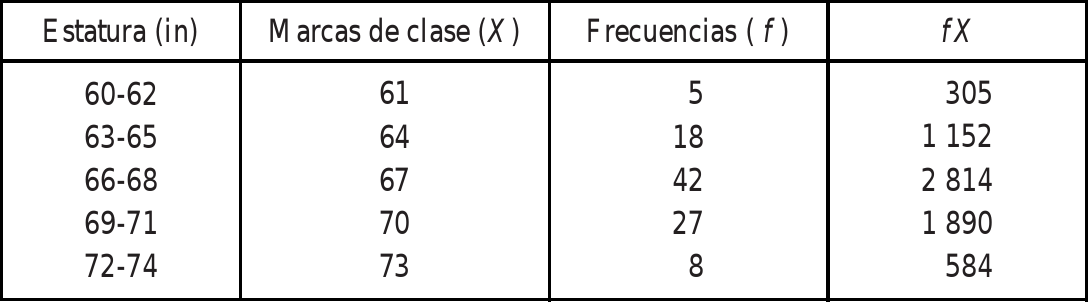
\includegraphics[width=10cm,keepaspectratio=true]{./images/tab0301.png}
		\label{tab:1.2.1-medidas}
	\end{figure}
\end{problema}

% Analizar
\begin{problema}
	\label{prob:08f4f21}
	Si las desviaciones de $N$ números $X_{1},..,X_{N}$ respecto a un \emph{pivote} arbitrario $P$ están dadas por $d_{i}=X_{i}-P, \; i=1,...,N$, demuestre algebraicamente que
	\begin{align}
		\bar{X}=P+\dfrac{\sum d_{i}}{N},
	\end{align}
	y verifique con este resultado que la fórmula anterior es válida sin importar qué valor de $P$ se elija.
\end{problema}

% Evaluar
\begin{problema}
	\label{prob:ced3c3b}
	Utilice la marca de la clase central como pivote y el método de codificación por cambio de escala y origen ($u_i = (X_i-P)/c$) para recalcular la estatura media de los 100 estudiantes del Problema \ref{prob:0c7ed43}. Compare el resultado y el esfuerzo aritmético contra el cálculo directo, y evalúe en qué situaciones (tamaño de la tabla, amplitud de clase, recursos de cómputo disponibles) conviene preferir el método codificado sobre el método directo.
\end{problema}

% Crear
\begin{problema}
	\label{prob:32476e7}
	Un analista registra el tiempo de respuesta (en milisegundos) de 60 solicitudes a un servidor web, agrupadas en la siguiente tabla de frecuencias:
	\begin{center}
		\begin{tabular}{cccc}
			\hline
			Intervalo (ms) & Marca de clase $X_i$ & Frecuencia $f_i$ & Frec. acumulada $F_i$ \\
			\hline
			10--19 & 14.5 & 6  & 6 \\
			20--29 & 24.5 & 14 & 20 \\
			30--39 & 34.5 & 22 & 42 \\
			40--49 & 44.5 & 12 & 54 \\
			50--59 & 54.5 & 6  & 60 \\
			\hline
		\end{tabular}
	\end{center}
	Diseñe la solución completa: calcule (a) el tiempo medio de respuesta $\bar{X}$ usando la marca de clase, y (b) el tiempo mediano de respuesta mediante interpolación lineal en la clase que contiene a la observación número $N/2=30$.
\end{problema}

\subsection*{Soluciones detalladas}

% Recordar
\begin{solproblema}[prob:f690fbe]
	Desarrollando término a término cada sumatoria según los índices indicados:
	\begin{enumerate}
		\item $\displaystyle\sum_{j=0}^{6}X_{j} = X_{0} + X_{1} + X_{2} + X_{3} + X_{4} + X_{5} + X_{6}$
		\item $\displaystyle\sum_{k=1}^{4}\left( Y_{k}-3 \right)^{2} = (Y_{1}-3)^{2} + (Y_{2}-3)^{2} + (Y_{3}-3)^{2} + (Y_{4}-3)^{2}$
		\item $\displaystyle\sum_{k=1}^{N}a = \underbrace{a + a + \cdots + a}_{N \text{ veces}} = N \cdot a$
		\item $\displaystyle\sum_{n=2}^{5}{f_{n}}X_{n} = f_{2}X_{2} + f_{3}X_{3} + f_{4}X_{4} + f_{5}X_{5}$
		\item $\displaystyle\sum_{m=0}^{3}\left( X_{m}-a \right) = (X_{0}-a) + (X_{1}-a) + (X_{2}-a) + (X_{3}-a)$
	\end{enumerate}
\end{solproblema}

% Comprender
\begin{solproblema}[prob:0b934f5]
	Sea $d_{i} = X_{i} - \bar{X}$. Sumando para todos los $N$ elementos del conjunto:
	\begin{align}
		\sum_{i=1}^{N} d_{i} &= \sum_{i=1}^{N} (X_{i} - \bar{X}) = \sum_{i=1}^{N} X_{i} - \sum_{i=1}^{N} \bar{X}.
	\end{align}
	Como $\bar{X}$ es una constante respecto al índice de sumatoria $i$, $\sum_{i=1}^{N} \bar{X} = N\bar{X}$. Además, por definición de media aritmética, $\sum_{i=1}^{N} X_{i} = N\bar{X}$. Sustituyendo ambos términos:
	\begin{align}
		\sum_{i=1}^{N} d_{i} = N\bar{X} - N\bar{X} = 0.
	\end{align}
	Esta propiedad justifica la interpretación física de la media como "centro de gravedad": así como el punto de equilibrio de un sistema de masas es aquel donde los momentos a ambos lados se cancelan, la media es el único pivote donde las desviaciones positivas y negativas de los datos se cancelan exactamente entre sí.
\end{solproblema}

% Aplicar
\begin{solproblema}[prob:0c7ed43]
	A partir de la tabla, determinamos el punto medio o marca de clase ($X_{i}$) para cada intervalo de estatura (en pulgadas) y multiplicamos por su frecuencia $f_{i}$:
	\begin{itemize}
		\item Intervalo 60--62: $X_{1} = 61$, $f_{1} = 5 \implies f_{1}X_{1} = 305$
		\item Intervalo 63--65: $X_{2} = 64$, $f_{2} = 18 \implies f_{2}X_{2} = 1152$
		\item Intervalo 66--68: $X_{3} = 67$, $f_{3} = 42 \implies f_{3}X_{3} = 2814$
		\item Intervalo 69--71: $X_{4} = 70$, $f_{4} = 27 \implies f_{4}X_{4} = 1890$
		\item Intervalo 72--74: $X_{5} = 73$, $f_{5} = 8 \implies f_{5}X_{5} = 584$
	\end{itemize}
	Sumando las frecuencias y los productos:
	\begin{align}
		N &= \sum f_{i} = 5 + 18 + 42 + 27 + 8 = 100 \\
		\sum f_{i}X_{i} &= 305 + 1152 + 2814 + 1890 + 584 = 6745
	\end{align}
	Por lo tanto, la estatura media es:
	\begin{align}
		\bar{X} = \dfrac{6745}{100} = 67.45 \text{ pulgadas.}
	\end{align}
\end{solproblema}

% Analizar
\begin{solproblema}[prob:08f4f21]
	Partimos de la definición de desviación respecto al pivote: $d_{i} = X_{i} - P$. Despejando la variable original tenemos $X_{i} = P + d_{i}$. Sumando desde $i=1$ hasta $N$ en ambos lados de la igualdad:
	\begin{align}
		\sum_{i=1}^{N} X_{i} &= \sum_{i=1}^{N} (P + d_{i}) = \sum_{i=1}^{N} P + \sum_{i=1}^{N} d_{i} = N \cdot P + \sum_{i=1}^{N} d_{i}.
	\end{align}
	Dividiendo toda la expresión entre $N$:
	\begin{align}
		\dfrac{\sum_{i=1}^{N} X_{i}}{N} &= \dfrac{N \cdot P}{N} + \dfrac{\sum_{i=1}^{N} d_{i}}{N} \implies \bar{X} = P + \dfrac{\sum_{i=1}^{N} d_{i}}{N}.
	\end{align}
	Esta derivación no impuso ninguna restricción sobre el valor de $P$: es válida para \emph{cualquier} pivote elegido, ya sea $P=0$, la media de otra muestra, o un valor arbitrario, siempre que $\sum d_i$ se recalcule respecto a ese mismo $P$. Esto es justamente lo que verifica numéricamente el resultado invariante $\bar{X}=9.375$ al usar $P=9$ o $P=20$ sobre el mismo conjunto de datos.
\end{solproblema}

% Evaluar
\begin{solproblema}[prob:ced3c3b]
	La marca de clase del intervalo central (66--68) es $P = 67$ pulgadas. Como las clases tienen un ancho constante $c = 3$ pulgadas, usamos la variable codificada $u_{i} = \dfrac{X_{i} - P}{c}$:
	\begin{itemize}
		\item Cl. 60--62 ($X_{1}=61$): $u_{1} = \frac{61-67}{3} = -2 \implies f_{1}u_{1} = 5(-2) = -10$
		\item Cl. 63--65 ($X_{2}=64$): $u_{2} = \frac{64-67}{3} = -1 \implies f_{2}u_{2} = 18(-1) = -18$
		\item Cl. 66--68 ($X_{3}=67$): $u_{3} = \frac{67-67}{3} = 0 \implies f_{3}u_{3} = 42(0) = 0$
		\item Cl. 69--71 ($X_{4}=70$): $u_{4} = \frac{70-67}{3} = 1 \implies f_{4}u_{4} = 27(1) = 27$
		\item Cl. 72--74 ($X_{5}=73$): $u_{5} = \frac{73-67}{3} = 2 \implies f_{5}u_{5} = 8(2) = 16$
	\end{itemize}
	Sumando las frecuencias por el código, $\sum f_{i}u_{i} = -10 - 18 + 0 + 27 + 16 = 15$. Aplicando la fórmula abreviada de la media con cambio de escala y origen:
	\begin{align}
		\bar{X} = P + c\left( \dfrac{\sum f_{i}u_{i}}{N} \right) = 67 + 3\left( \dfrac{15}{100} \right) = 67.45 \text{ pulgadas,}
	\end{align}
	idéntico al resultado directo del Problema \ref{prob:0c7ed43}. En cuanto al esfuerzo aritmético, el método codificado reemplaza productos de números grandes (marca de clase $\times$ frecuencia, valores de dos y tres cifras) por productos de enteros pequeños ($-2$ a $2$), lo cual reduce el riesgo de error de cálculo manual. Sin embargo, con software o calculadoras estadísticas la ventaja desaparece casi por completo, ya que ambos métodos son igual de rápidos de ejecutar. El método codificado conviene, entonces, principalmente en cálculo manual con tablas grandes o amplitud de clase constante, no como sustituto sistemático en un flujo de trabajo computarizado.
\end{solproblema}

% Crear
\begin{solproblema}[prob:32476e7]
	\textbf{(a) Media aritmética.} Multiplicando cada marca de clase por su frecuencia:
	\begin{align}
		\sum f_iX_i = 6(14.5)+14(24.5)+22(34.5)+12(44.5)+6(54.5) = 87+343+759+534+327 = 2050.
	\end{align}
	Con $N=60$:
	\begin{align}
		\bar{X} = \dfrac{2050}{60} \approx 34.17 \text{ ms.}
	\end{align}
	\textbf{(b) Mediana por interpolación.} Buscamos la clase que contiene a la observación $N/2=30$: la frecuencia acumulada llega a $F=20$ al final de la clase 20--29 y a $F=42$ al final de la clase 30--39, así que la clase mediana es 30--39, con límite real inferior $L_m=29.5$, frecuencia acumulada anterior $F_{m-1}=20$, frecuencia de la clase $f_m=22$ y amplitud $c=10$:
	\begin{align}
		Med = L_m + \left( \dfrac{N/2 - F_{m-1}}{f_m} \right)c = 29.5 + \left( \dfrac{30-20}{22} \right)(10) = 29.5 + 4.55 = 34.05 \text{ ms.}
	\end{align}
	La media ($34.17$ ms) y la mediana ($34.05$ ms) resultan muy cercanas entre sí, lo cual es consistente con una distribución de tiempos de respuesta razonablemente simétrica alrededor de la clase central.
\end{solproblema}

\section{Medidas de dispersión}

\subsection{Dispersión o variación}
Si bien las medidas de tendencia central nos dicen alrededor de qué valores se concentra un arreglo de datos, las \emph{medidas de dispersión} nos dan una idea de qué tan alejados están los datos entre sí y respecto a la media.

\begin{observacion}
	Dos conjuntos de datos pueden tener la misma media pero muy distinta dispersión. Por ejemplo, los conjuntos $\{49, 50, 51\}$ y $\{0, 50, 100\}$ tienen la misma media ($\bar{X} = 50$), pero claramente el segundo está mucho más disperso.
\end{observacion}

A continuación veremos algunas medidas de dispersión comúnmente usadas en estadística.

\subsection{Rango}
El \emph{rango} de un conjunto de datos es la diferencia entre el mayor y el menor valor del conjunto.

\begin{ejemplo}
	El rango del conjunto $2,3,3,5,5,5,8,10,12$ es $12-2=10.$
\end{ejemplo}

\begin{observacion}
	El rango es la medida de dispersión más simple, pero tiene la desventaja de depender únicamente de los valores extremos, ignorando la distribución de los datos intermedios.
\end{observacion}


\subsection{Desviación media}
La \emph{desviación media} o \emph{desviación promedio} de un conjunto de $N$ números $X_{1},...,X_{N}$ está definida como
\begin{align}
	DM=\dfrac{\sum \abs{X_{j}-\bar{X}}}{N}
\end{align}
donde $\bar{X}$ es la media aritmética de los números y $\abs{\cdot}$ denota el valor absoluto.

\begin{ejemplo}
	Encuentre la desviación media de la lista $2,3,6,8,11.$
\end{ejemplo}

\begin{solucion}
	Primero calculamos la media:
	\begin{align}
		\bar{X} = \frac{2+3+6+8+11}{5} = \frac{30}{5} = 6
	\end{align}
	
	Luego calculamos las desviaciones absolutas respecto a la media:
	\begin{align}
		DM &= \frac{|2-6| + |3-6| + |6-6| + |8-6| + |11-6|}{5} \\
		&= \frac{4 + 3 + 0 + 2 + 5}{5} = \frac{14}{5} = 2.8
	\end{align}
\end{solucion}


\subsection{Desviación estándar}
La \emph{desviación estándar} de un conjunto de $N$ números $X_{1},...,X_{N}$ se denota como $s$ y está definida por
\begin{align}
	s=\sqrt{\dfrac{\sum\left( X_{j}-\bar{X} \right)^{2}}{N}}=\sqrt{\sum\dfrac{x_{j}^{2}}{N}}
\end{align} donde $x_{j}:=X_{j}-\bar{X}.$

\begin{observacion}
	La desviación estándar mide qué tan dispersos están los datos respecto a la media. Una desviación estándar pequeña indica que los datos están concentrados cerca de la media, mientras que una desviación estándar grande indica que los datos están muy dispersos.
\end{observacion}

Si $X_{1},...,X_{N}$ se presentan con frecuencias $f_{1},...,f_{N}$ respectivamente, la desviación estándar se puede expresar como
\begin{align}
	s=\sqrt{\dfrac{\sum f_{j}\left( X_{j}-\bar{X} \right)^{2}}{N}}=\sqrt{\dfrac{\sum f_{j}x_{j}^{2}}{N}}
\end{align}

\begin{ejemplo}
	Calcule la desviación estándar del conjunto $2, 4, 4, 4, 5, 5, 7, 9.$
\end{ejemplo}

\begin{solucion}
	Primero calculamos la media:
	\begin{align}
		\bar{X} = \frac{2+4+4+4+5+5+7+9}{8} = \frac{40}{8} = 5
	\end{align}
	
	Luego calculamos las desviaciones al cuadrado:
	\begin{align}
		(2-5)^2 &= 9 \\
		(4-5)^2 &= 1 \quad (\text{tres veces}) \\
		(5-5)^2 &= 0 \quad (\text{dos veces}) \\
		(7-5)^2 &= 4 \\
		(9-5)^2 &= 16
	\end{align}
	
	Por lo tanto:
	\begin{align}
		s &= \sqrt{\frac{9 + 3(1) + 2(0) + 4 + 16}{8}} = \sqrt{\frac{32}{8}} = \sqrt{4} = 2
	\end{align}
\end{solucion}


\subsection{Varianza}
La \emph{varianza} de un conjunto de números se define como el cuadrado $s^{2}$ de la desviación estándar $s$.

\begin{observacion}
	En estadística es importante distinguir entre la desviación estándar de una \emph{población} y de una \emph{muestra}. Para distinguirlas, en el primer caso utilizaremos $\sigma$ y en el segundo continuaremos usando $s.$
	
	Cuando trabajamos con una muestra y queremos estimar la varianza poblacional, utilizamos $N-1$ en lugar de $N$ como denominador:
	\begin{align}
		s^2 = \frac{\sum (X_j - \bar{X})^2}{N-1}
	\end{align}
	
	Esta corrección (llamada \emph{corrección de Bessel}) produce un estimador insesgado de la varianza poblacional. Para muestras grandes ($N > 30$), la diferencia entre usar $N$ y $N-1$ es prácticamente despreciable.
\end{observacion}


\subsection{Método abreviado}
Una forma computacionalmente más eficiente de calcular la varianza es:
\begin{align}
	s^{2} &= \overline{X^{2}} - \overline{X}^{2} \\
	&= \frac{\sum X_j^2}{N} - \left(\frac{\sum X_j}{N}\right)^2
\end{align}

donde $\overline{X^2}$ denota la media de los cuadrados y $\overline{X}^2$ denota el cuadrado de la media.

\begin{observacion}
	Esta fórmula es equivalente a la definición original pero evita calcular las desviaciones individuales. Es particularmente útil para cálculos manuales o cuando se trabaja con datos agrupados.
\end{observacion}


\subsection{Coeficiente de variación}
El \emph{coeficiente de variación} es una medida de dispersión relativa que permite comparar la variabilidad de conjuntos de datos con diferentes unidades o escalas:
\begin{align}
	CV = \frac{s}{\bar{X}} \times 100\%
\end{align}

\begin{ejemplo}
	Compare la variabilidad de las estaturas y pesos de un grupo de personas:
	\begin{itemize}
		\item Estaturas: $\bar{X} = 170$ cm, $s = 8$ cm
		\item Pesos: $\bar{X} = 70$ kg, $s = 10$ kg
	\end{itemize}
\end{ejemplo}

\begin{solucion}
	\begin{align}
		CV_{\text{estatura}} &= \frac{8}{170} \times 100\% \approx 4.71\% \\
		CV_{\text{peso}} &= \frac{10}{70} \times 100\% \approx 14.29\%
	\end{align}
	
	Aunque la desviación estándar del peso ($10$ kg) es mayor que la de la estatura ($8$ cm) en valor absoluto, el coeficiente de variación nos muestra que el peso tiene mucha mayor variabilidad relativa ($14.29\%$ vs $4.71\%$).
\end{solucion}


\subsection{Varianza de conjuntos combinados}
Si dos conjuntos de $N_{1}$ y $N_{2}$ datos respectivamente tienen correspondientes varianzas $s_{1}^{2}$ y $s_{2}^{2}$ pero una misma media aritmética $\bar{X},$ entonces la varianza del conjunto combinado es
\begin{align}
	s^{2}=\dfrac{N_{1}s_{1}^{2}+N_{2}s_{2}^{2}}{N_{1}+N_{2}}.
\end{align}


\subsection{Teorema de Chebyshev}

\begin{teorema}[Chebyshev]
	Para cualquier variable aleatoria $X$ con media $\mu$ y desviación estándar $\sigma$, y para cualquier $k > 1$,
	\begin{align}
		P(|X - \mu| < k\sigma) \geq 1 - \frac{1}{k^2}
	\end{align}
	
	Es decir, por lo menos $1 - \frac{1}{k^2}$ de la distribución de probabilidad de $X$ está a no más de $k$ desviaciones estándar de la media.
\end{teorema}

\begin{proof}
	Demostraremos el teorema para el caso discreto. Sea $f(x)$ la función de probabilidad de $X$.
	
	La varianza es:
	\begin{align}
		\sigma^2 = \sum_{x} (x - \mu)^2 f(x)
	\end{align}
	
	Separamos la suma en dos partes: valores dentro de $k\sigma$ de la media y valores fuera:
	\begin{align}
		\sigma^2 &= \sum_{|x-\mu| < k\sigma} (x-\mu)^2 f(x) + \sum_{|x-\mu| \geq k\sigma} (x-\mu)^2 f(x)
	\end{align}
	
	La primera suma es no negativa, así que:
	\begin{align}
		\sigma^2 \geq \sum_{|x-\mu| \geq k\sigma} (x-\mu)^2 f(x)
	\end{align}
	
	Para los términos en la segunda suma, $(x-\mu)^2 \geq k^2\sigma^2$, por lo que:
	\begin{align}
		\sigma^2 &\geq \sum_{|x-\mu| \geq k\sigma} k^2\sigma^2 f(x) = k^2\sigma^2 \sum_{|x-\mu| \geq k\sigma} f(x) \\
		&= k^2\sigma^2 P(|X-\mu| \geq k\sigma)
	\end{align}
	
	Dividiendo entre $k^2\sigma^2$:
	\begin{align}
		P(|X-\mu| \geq k\sigma) \leq \frac{1}{k^2}
	\end{align}
	
	Por lo tanto:
	\begin{align}
		P(|X-\mu| < k\sigma) = 1 - P(|X-\mu| \geq k\sigma) \geq 1 - \frac{1}{k^2}
	\end{align}
\end{proof}

\begin{observacion}
	Para $k=2$, el teorema garantiza que al menos $1 - \frac{1}{4} = 75\%$ de los datos están dentro de 2 desviaciones estándar de la media. Para $k=3$, al menos $1 - \frac{1}{9} \approx 88.9\%$ están dentro de 3 desviaciones estándar.
	
	En distribuciones normales, estos porcentajes son mucho mayores: $95.45\%$ dentro de $\pm 2\sigma$ y $99.73\%$ dentro de $\pm 3\sigma$.
\end{observacion}


\subsection{Python}

\texttt{Numpy} proporciona funciones para calcular todas las medidas de dispersión:

\begin{lstlisting}[language=Python]
import numpy as np

data = np.array([2, 4, 4, 4, 5, 5, 7, 9])

# Rango
rango = np.ptp(data)
print(f"Rango: {rango}")  # 7

# Desviación media
desv_media = np.mean(np.abs(data - np.mean(data)))
print(f"Desviación media: {desv_media}")  # 1.5

# Desviación estándar (poblacional, ddof=0)
std_pop = np.std(data, ddof=0)
print(f"Desviación estándar poblacional: {std_pop}")  # 2.0

# Desviación estándar (muestral, ddof=1)
std_muestra = np.std(data, ddof=1)
print(f"Desviación estándar muestral: {std_muestra}")  # 2.138

# Varianza
var_pop = np.var(data, ddof=0)
print(f"Varianza poblacional: {var_pop}")  # 4.0

var_muestra = np.var(data, ddof=1)
print(f"Varianza muestral: {var_muestra}")  # 4.571

# Coeficiente de variación
cv = (std_pop / np.mean(data)) * 100
print(f"Coeficiente de variación: {cv:.2f}%")  # 40.00%
\end{lstlisting}

\begin{observacion}
	El parámetro \texttt{ddof} (Delta Degrees of Freedom) controla el denominador: \texttt{ddof=0} usa $N$ (poblacional) y \texttt{ddof=1} usa $N-1$ (muestral).
\end{observacion}

\section*{Problemas}

\subsection*{Enunciados de los problemas}

% Recordar
\begin{problema}
	\label{prob:ba2e465}
	Encontrar el rango y las desviaciones media y estándar de los siguientes arreglos de datos no agrupados:
	\begin{enumerate}
		\item $12, 6, 7, 3, 15, 10, 18, 5$
		\item $9, 3, 8, 8, 9, 8, 9, 18.$
	\end{enumerate}
	Compruebe sus resultados con \texttt{Python}.
\end{problema}

% Comprender
\begin{problema}
	\label{prob:c5833ad}
	Si $d=X-P$ representan las desviaciones de una variable $X$ respecto a un pivote constante $P$, demuestre que la desviación estándar es invariante ante traslaciones —es decir, que su valor no depende de qué pivote $P$ se elija— y explique por qué esta propiedad es deseable para una medida de dispersión.
\end{problema}

% Aplicar
\begin{problema}
	\label{prob:d87f55c}
	Dos grupos de estudiantes tienen las siguientes características muestrales:
	\begin{itemize}
		\item Grupo A: $n_1 = 30$ estudiantes, $\bar{X}_1 = 75$ puntos, $s_1 = 8$ puntos
		\item Grupo B: $n_2 = 20$ estudiantes, $\bar{X}_2 = 75$ puntos, $s_2 = 12$ puntos
	\end{itemize}
	Encuentre la desviación estándar del grupo combinado de $n_1 + n_2 = 50$ estudiantes.
\end{problema}

% Analizar
\begin{problema}
	\label{prob:6112df0}
	Demuestre rigurosamente que para cualquier conjunto de datos (no agrupados o agrupados):
	\begin{align}
		s &= \sqrt{\dfrac{\sum X^{2}}{N}-\left( \dfrac{\sum X}{N} \right)^{2}} = \sqrt{\overline{X^{2}}-\overline{X}^{2}}\\
		s &= \sqrt{\dfrac{\sum fX^{2}}{N}-\left( \dfrac{\sum fX}{N} \right)^{2}} = \sqrt{\overline{X^{2}}-\overline{X}^{2}}
	\end{align}
\end{problema}

% Evaluar
\begin{problema}
	\label{prob:dd18a2e}
	El coeficiente de variación se define como $CV = (s/\bar{X}) \times 100\%$. Compare e interprete la variabilidad relativa en las siguientes dos situaciones prácticas:
	\begin{itemize}
		\item Los salarios de dos empresas: Empresa A tiene $\bar{X}_A = \$45,000$ y $s_A = \$8,000$; Empresa B tiene $\bar{X}_B = \$38,000$ y $s_B = \$6,500$.
		\item Las estaturas y pesos de un grupo antropométrico: estatura media $170$ cm con $s = 8$ cm; peso medio $70$ kg con $s = 10$ kg.
	\end{itemize}
	Evalúe en cada caso cuál de las dos cantidades comparadas exhibe mayor dispersión relativa, y explique por qué la desviación estándar sola (sin dividir entre la media) sería insuficiente para esta comparación.
\end{problema}

% Crear
\begin{problema}
	\label{prob:78de91c}
	Un analista de calidad agrupa el peso (en gramos) de 50 piezas manufacturadas en la siguiente tabla, con amplitud de clase constante $c=4$ y pivote en la marca de la clase central $P=52$:
	\begin{center}
		\begin{tabular}{ccc}
			\hline
			Marca de clase $X_i$ & Frecuencia $f_i$ & $u_i=(X_i-P)/c$ \\
			\hline
			44 & 4  & $-2$ \\
			48 & 10 & $-1$ \\
			52 & 20 & $0$ \\
			56 & 12 & $1$ \\
			60 & 4  & $2$ \\
			\hline
		\end{tabular}
	\end{center}
	Diseñe la solución completa usando el método de cambio de escala y origen ($s = c \cdot s_u$): calcule $s_u$ a partir de la columna $u_i$ y úselo para obtener la desviación estándar $s$ del peso de las piezas en gramos.
\end{problema}

\subsection*{Soluciones detalladas}

% Recordar
\begin{solproblema}[prob:ba2e465]
	\begin{enumerate}
		\item Para el arreglo $12,6,7,3,15,10,18,5$:
		\begin{itemize}
			\item \textbf{Rango:} $\max - \min = 18 - 3 = 15$
			\item \textbf{Media:} $\bar{X} = \frac{12+6+7+3+15+10+18+5}{8} = \frac{76}{8} = 9.5$
			\item \textbf{Desviación media ($DM$):}
			\begin{align}
				DM &= \frac{|12-9.5| + |6-9.5| + |7-9.5| + |3-9.5| + |15-9.5| + |10-9.5| + |18-9.5| + |5-9.5|}{8} \\
				&= \frac{2.5 + 3.5 + 2.5 + 6.5 + 5.5 + 0.5 + 8.5 + 4.5}{8} = \frac{34}{8} = 4.25
			\end{align}
			\item \textbf{Desviación estándar ($s$):}
			\begin{align}
				s &= \sqrt{\frac{(12-9.5)^2 + (6-9.5)^2 + (7-9.5)^2 + (3-9.5)^2 + (15-9.5)^2 + (10-9.5)^2 + (18-9.5)^2 + (5-9.5)^2}{8}} \\
				&= \sqrt{\frac{6.25 + 12.25 + 6.25 + 42.25 + 30.25 + 0.25 + 72.25 + 20.25}{8}} = \sqrt{\frac{190}{8}} = \sqrt{23.75} \approx 4.87
			\end{align}
		\end{itemize}

		\item Para el arreglo $9,3,8,8,9,8,9,18$:
		\begin{itemize}
			\item \textbf{Rango:} $18 - 3 = 15$
			\item \textbf{Media:} $\bar{X} = \frac{9+3+8+8+9+8+9+18}{8} = \frac{72}{8} = 9$
			\item \textbf{Desviación media ($DM$):}
			\begin{align}
				DM &= \frac{|9-9| + |3-9| + |8-9| + |8-9| + |9-9| + |8-9| + |9-9| + |18-9|}{8} \\
				&= \frac{0 + 6 + 1 + 1 + 0 + 1 + 0 + 9}{8} = \frac{18}{8} = 2.25
			\end{align}
			\item \textbf{Desviación estándar ($s$):}
			\begin{align}
				s &= \sqrt{\frac{0^2 + (-6)^2 + (-1)^2 + (-1)^2 + 0^2 + (-1)^2 + 0^2 + 9^2}{8}} = \sqrt{\frac{120}{8}} = \sqrt{15} \approx 3.87
			\end{align}
		\end{itemize}
	\end{enumerate}
\end{solproblema}

\begin{lstlisting}[language=Python]
import numpy as np
# Conjunto 1
data1 = np.array([12, 6, 7, 3, 15, 10, 18, 5])
print("Conjunto 1:")
print(f"Rango: {np.ptp(data1)}")
print(f"Media: {np.mean(data1)}")
print(f"Desviación media: {np.mean(np.abs(data1 - np.mean(data1)))}")
print(f"Desviación estándar: {np.std(data1)}")
# Conjunto 2
data2 = np.array([9, 3, 8, 8, 9, 8, 9, 18])
print("\nConjunto 2:")
print(f"Rango: {np.ptp(data2)}")
print(f"Media: {np.mean(data2)}")
print(f"Desviación media: {np.mean(np.abs(data2 - np.mean(data2)))}")
print(f"Desviación estándar: {np.std(data2)}")
\end{lstlisting}

% Comprender
\begin{solproblema}[prob:c5833ad]
	Si $d_j = X_j - P$, entonces $X_j = d_j + P$. La media de $X$ en términos del pivote es:
	\begin{align}
		\bar{X} = \frac{\sum f_j X_j}{N} = \frac{\sum f_j (d_j + P)}{N} = \frac{\sum f_j d_j}{N} + P = \bar{d} + P.
	\end{align}
	La desviación respecto a la media se transforma según:
	\begin{align}
		X_j - \bar{X} = (d_j + P) - (\bar{d} + P) = d_j - \bar{d}.
	\end{align}
	El término $P$ se cancela exactamente, así que la varianza resulta idéntica sea cual sea el pivote elegido:
	\begin{align}
		s^2 = \frac{\sum f_j (X_j - \bar{X})^2}{N} = \frac{\sum f_j (d_j - \bar{d})^2}{N}.
	\end{align}
	Esta invarianza es deseable porque la dispersión de un conjunto de datos es una propiedad intrínseca de qué tan alejados están los datos entre sí, no de dónde se coloque arbitrariamente el origen de medición: trasladar todos los datos (cambiar unidades de referencia, restar una constante) no debe alterar cuánto varían entre sí.
\end{solproblema}

% Aplicar
\begin{solproblema}[prob:d87f55c]
	Como ambos grupos tienen la misma media ($\bar{X}_1 = \bar{X}_2 = 75$), la media combinada es también $\bar{X} = 75$. En este caso sin diferencia entre medias de grupo, la varianza combinada es el promedio ponderado de las varianzas individuales:
	\begin{align}
		s^2 &= \frac{n_1 s_1^2 + n_2 s_2^2}{n_1 + n_2} = \frac{30 \cdot 8^2 + 20 \cdot 12^2}{30 + 20} \\
		&= \frac{30 \cdot 64 + 20 \cdot 144}{50} = \frac{1920 + 2880}{50} = \frac{4800}{50} = 96
	\end{align}
	Por lo tanto, la desviación estándar del grupo combinado es:
	\begin{align}
		s = \sqrt{96} \approx 9.80 \text{ puntos.}
	\end{align}
\end{solproblema}

% Analizar
\begin{solproblema}[prob:6112df0]
	Partimos de la definición formal de varianza muestral (o poblacional dividida entre $N$):
	\begin{align}
		s^2 &= \frac{\sum (X_j - \bar{X})^2}{N} = \frac{\sum (X_j^2 - 2X_j\bar{X} + \bar{X}^2)}{N} \\
		&= \frac{\sum X_j^2 - 2\bar{X}\sum X_j + N\bar{X}^2}{N} = \frac{\sum X_j^2}{N} - 2\bar{X}\frac{\sum X_j}{N} + \bar{X}^2 \\
		&= \frac{\sum X_j^2}{N} - 2\bar{X}\cdot\bar{X} + \bar{X}^2 = \frac{\sum X_j^2}{N} - \bar{X}^2 = \overline{X^2} - \overline{X}^2.
	\end{align}
	Tomando la raíz cuadrada a ambos lados, se demuestra la identidad:
	\begin{align}
		s = \sqrt{\overline{X^2} - \overline{X}^2}.
	\end{align}
	Para datos con frecuencias, el mismo razonamiento algebraico es válido al reemplazar $\sum X_j^2$ por $\sum f_j X_j^2$ y $\sum X_j$ por $\sum f_j X_j$, ya que $N=\sum f_j$ y $\sum f_j$ actúa como el número total de observaciones ponderadas.
\end{solproblema}

% Evaluar
\begin{solproblema}[prob:dd18a2e]
	\textbf{Salarios:}
	\begin{align}
		CV_A &= \frac{8000}{45000} \times 100\% \approx 17.78\% \\
		CV_B &= \frac{6500}{38000} \times 100\% \approx 17.11\%
	\end{align}
	Ambas empresas muestran una dispersión salarial relativa prácticamente similar (alrededor del 17\%), aunque la Empresa A tiene una variabilidad ligeramente mayor en relación con el monto de su nómina promedio. Comparar directamente $s_A=\$8{,}000$ contra $s_B=\$6{,}500$ sería engañoso, porque ignora que la Empresa A también paga salarios promedio más altos.

	\textbf{Estaturas vs. pesos:}
	\begin{align}
		CV_{\text{estatura}} &= \frac{8}{170} \times 100\% \approx 4.71\% \\
		CV_{\text{peso}} &= \frac{10}{70} \times 100\% \approx 14.29\%
	\end{align}
	A pesar de que las unidades físicas son distintas (cm vs.\ kg), el coeficiente de variación permite su comparación adimensional directa. Se concluye que el peso presenta el triple de variabilidad relativa que la estatura en dicha población. En ambos casos, la desviación estándar sola es insuficiente para comparar porque mezcla la escala absoluta de la variable con su dispersión: dos variables con la misma $s$ pero medias muy distintas (o medidas en unidades distintas, como cm y kg) no son comparables en términos de variabilidad relativa sin normalizar por la media.
\end{solproblema}

% Crear
\begin{solproblema}[prob:78de91c]
	Con $N=\sum f_i = 4+10+20+12+4=50$, calculamos $\sum f_iu_i$ y $\sum f_iu_i^2$:
	\begin{align}
		\sum f_iu_i &= 4(-2)+10(-1)+20(0)+12(1)+4(2) = -8-10+0+12+8 = 2 \\
		\sum f_iu_i^2 &= 4(4)+10(1)+20(0)+12(1)+4(4) = 16+10+0+12+16 = 54
	\end{align}
	La desviación estándar codificada es:
	\begin{align}
		s_u = \sqrt{\dfrac{\sum f_iu_i^2}{N} - \left(\dfrac{\sum f_iu_i}{N}\right)^2} = \sqrt{\dfrac{54}{50} - \left(\dfrac{2}{50}\right)^2} = \sqrt{1.08 - 0.0016} = \sqrt{1.0784} \approx 1.0385.
	\end{align}
	Aplicando el cambio de escala $s = c \cdot s_u$ con $c=4$:
	\begin{align}
		s = 4 \times 1.0385 \approx 4.15 \text{ gramos.}
	\end{align}
	El método codificado evita manejar directamente los valores grandes de la marca de clase (44 a 60), operando en su lugar con enteros pequeños ($-2$ a $2$).
\end{solproblema}


%%%%%%%%%%%%%%%%%%%%%%%%%%%%%%
% UNIDAD 1 DEL TEMARIO
\chapter{Teoría de Probabilidad}
\section*{Introducción a la probabilidad}

La \emph{probabilidad} es la rama de las matemáticas que estudia los fenómenos aleatorios, es decir, aquellos cuyos resultados no pueden determinarse de antemano con certeza. A diferencia de los fenómenos deterministas (como la caída de un objeto bajo la gravedad), los fenómenos aleatorios presentan variabilidad inherente que solo puede describirse mediante modelos probabilísticos.

\subsection*{¿Por qué estudiar probabilidad?}

La probabilidad es fundamental en múltiples áreas del conocimiento:

\begin{itemize}
	\item \textbf{Ciencias naturales:} Modelado de fenómenos cuánticos, genética, evolución, termodinámica estadística.
	\item \textbf{Ingeniería:} Confiabilidad de sistemas, teoría de colas, procesamiento de señales.
	\item \textbf{Economía y finanzas:} Valoración de opciones, gestión de riesgos, modelos de mercado.
	\item \textbf{Ciencias de la computación:} Algoritmos aleatorizados, aprendizaje automático, criptografía.
	\item \textbf{Medicina:} Ensayos clínicos, epidemiología, diagnóstico probabilístico.
	\item \textbf{Vida cotidiana:} Toma de decisiones bajo incertidumbre, juegos de azar, predicciones meteorológicas.
\end{itemize}

\subsection*{Relación con la estadística}

La probabilidad y la estadística están íntimamente relacionadas:

\begin{itemize}
	\item La \textbf{probabilidad} proporciona el marco teórico para modelar fenómenos aleatorios y calcular la likelihood de eventos.
	\item La \textbf{estadística inferencial} utiliza datos observados para hacer inferencias sobre poblaciones, utilizando los modelos probabilísticos como fundamento.
\end{itemize}

En otras palabras, la probabilidad nos dice qué tan probable es observar ciertos datos dado un modelo, mientras que la estadística nos ayuda a inferir el modelo a partir de los datos observados.

\subsection*{Conceptos fundamentales}

En este capítulo desarrollaremos los siguientes conceptos:

\begin{enumerate}
	\item \textbf{Experimentos aleatorios y espacio muestral:} Definiremos qué es un experimento aleatorio y cómo describir todos sus posibles resultados.
	\item \textbf{Eventos y operaciones:} Estudiaremos cómo combinar eventos mediante unión, intersección y complemento.
	\item \textbf{Axiomas de probabilidad:} Presentaremos el enfoque axiomático moderno de Kolmogorov.
	\item \textbf{Probabilidad condicional e independencia:} Analizaremos cómo la ocurrencia de un evento afecta la probabilidad de otro.
	\item \textbf{Teorema de Bayes:} Una herramienta fundamental para actualizar probabilidades con nueva información.
	\item \textbf{Variables aleatorias:} Funciones que asignan valores numéricos a los resultados de experimentos aleatorios.
	\item \textbf{Distribuciones especiales:} Modelos probabilísticos comúnmente utilizados (binomial, normal, Poisson).
\end{enumerate}

\subsection*{Un poco de historia}

El estudio matemático de la probabilidad comenzó en el siglo XVII con correspondencia entre Blaise Pascal y Pierre de Fermat sobre problemas de juegos de azar. Posteriormente, Jacob Bernoulli demostró la Ley de los Grandes Números, y en el siglo XX, Andrey Kolmogorov estableció los axiomas modernos de la probabilidad en 1933, proporcionando una base matemática rigurosa.

\begin{observacion}
	A lo largo de este capítulo, utilizaremos ejemplos concretos (lanzamiento de monedas, dados, extracción de cartas) para ilustrar los conceptos. Sin embargo, estos mismos principios se aplican a problemas mucho más complejos en ciencia, ingeniería y toma de decisiones.
\end{observacion}

\input{conjuntos}
\section*{Problemas}

\subsection*{Enunciados de los problemas}

% Recordar
\begin{problema}
	\label{prob:b94325d}
	Sea el espacio muestral $S$ y dos subconjuntos $A, B \subset S$. Enumera explícitamente los $2^2 = 4$ elementos disjuntos que conforman la partición fundamental $\particion(A,B)$ del espacio $S$.
\end{problema}

% Comprender
\begin{problema}
	\label{prob:320d62d}
	Extiende la construcción de una partición al caso de tres subconjuntos $A, B, C \subset S$. ¿Cuántos elementos tiene la partición $\particion(A,B,C)$ y cuáles son explícitamente estos subconjuntos elementales disjuntos? Explica por qué el número de elementos se duplica al agregar un tercer conjunto.
\end{problema}

% Aplicar
\begin{problema}
	\label{prob:18eada9}
	En un grupo de 50 estudiantes, 35 practican fútbol, 25 practican básquetbol y 15 practican ambos deportes. Usando las variables de la partición fundamental $\particion(F,B)$, ¿cuántos estudiantes no practican ningún deporte?
\end{problema}

% Analizar
\begin{problema}
	\label{prob:6d1bd44}
	Utilizando el principio de inclusión-exclusión o la teoría de particiones, demuestra la identidad de cardinalidad para la unión de tres conjuntos $A, B, C \subset S$:
	\begin{align}
		\card{A \cup B \cup C} = \card{A} + \card{B} + \card{C} - \card{A \cap B} - \card{A \cap C} - \card{B \cap C} + \card{A \cap B \cap C}.
	\end{align}
\end{problema}

% Evaluar
\begin{problema}
	\label{prob:15ead08}
	Un equipo de analistas en un ensayo clínico epidemiológico con un total de $\card{S} = 500$ pacientes evaluó la presencia de tres síntomas de una patología nueva ($S_1, S_2, S_3$). El informe preliminar presenta la siguiente estadística censal:
	\begin{itemize}
		\item $\card{S_1} = 300, \quad \card{S_2} = 250, \quad \card{S_3} = 200$
		\item $\card{S_1 \cap S_2} = 180, \quad \card{S_1 \cap S_3} = 150, \quad \card{S_2 \cap S_3} = 130$
		\item $\card{S_1 \cap S_2 \cap S_3} = 30$
	\end{itemize}
	Mediante el desglose algebraico en los 8 elementos de la partición $\particion(S_1,S_2,S_3)$, evalúa rigurosamente por qué el informe contiene un error lógico inevitable que imposibilita que estos datos correspondan a un censo real. Identifica específicamente cuál elemento de la partición arroja una cardinalidad matemáticamente absurda.
\end{problema}

% Crear
\begin{problema}
	\label{prob:95d5458}
	Un equipo de producto en una app de streaming musical clasifica a sus 800 usuarios activos según tres hábitos de consumo: escuchan \emph{podcasts} ($P$), crean listas de reproducción propias ($L$) y usan el modo sin conexión ($O$). Diseñe un ejemplo original con cardinalidades hipotéticas para $\card{P}$, $\card{L}$, $\card{O}$ y sus intersecciones (simples, dobles y triple) tales que los datos sean lógicamente consistentes (a diferencia del problema del ensayo clínico). Calcule, mediante el desglose en los 8 elementos de $\particion(P,L,O)$, cuántos usuarios no tienen ninguno de los tres hábitos.
\end{problema}

\subsection*{Soluciones detalladas}

% Recordar
\begin{solproblema}[prob:b94325d]
	Para dos subconjuntos $A, B \subset S$, cada elemento del espacio $S$ puede pertenecer o no pertenecer (complemento) a cada uno de los dos conjuntos. Esto genera $2 \times 2 = 4$ intersecciones elementales mutuamente disjuntas cuya unión totaliza al espacio $S$:
	\begin{itemize}
		\item $E_0 = A' \cap B'$ (elementos exteriores a ambos conjuntos)
		\item $E_1 = A' \cap B$ (elementos exclusivos de $B$)
		\item $E_2 = A \cap B'$ (elementos exclusivos de $A$)
		\item $E_3 = A \cap B$ (elementos en la intersección común de ambos)
	\end{itemize}
	Por construcción, se verifica que $E_i \cap E_j = \emptyset$ para todo $i \neq j$ y que $\bigcup_{k=0}^3 E_k = S$.
\end{solproblema}

% Comprender
\begin{solproblema}[prob:320d62d]
	Para tres subconjuntos $A, B, C \subset S$, al incluir la membresía dual o binaria respecto a un tercer conjunto $C$ o su complemento $C'$, el número de regiones se duplica respecto al caso de dos conjuntos: $2^3 = 8$ elementos elementales disjuntos.

	Estos 8 subconjuntos, ordenados sistemáticamente en código binario (donde pertenecer al conjunto activa un bit y pertenecer al complemento lo apaga), son:
	\begin{itemize}
		\item $E_0 = A' \cap B' \cap C'$ (ninguno de los tres conjuntos)
		\item $E_1 = A' \cap B' \cap C$ (sólamente en $C$)
		\item $E_2 = A' \cap B \cap C'$ (sólamente en $B$)
		\item $E_3 = A' \cap B \cap C$ (simultáneamente en $B$ y $C$, pero no en $A$)
		\item $E_4 = A \cap B' \cap C'$ (sólamente en $A$)
		\item $E_5 = A \cap B' \cap C$ (simultáneamente en $A$ y $C$, pero no en $B$)
		\item $E_6 = A \cap B \cap C'$ (simultáneamente en $A$ y $B$, pero no en $C$)
		\item $E_7 = A \cap B \cap C$ (en la intersección simultánea de los tres conjuntos)
	\end{itemize}
	El número se duplica porque cada nuevo conjunto añade un bit binario independiente (pertenece / no pertenece) a la codificación de cada región: pasar de 2 a 3 conjuntos multiplica por 2 el número de combinaciones posibles, de $2^2=4$ a $2^3=8$.
\end{solproblema}

% Aplicar
\begin{solproblema}[prob:18eada9]
	Sea $F$ la colección de estudiantes que practican fútbol y $B$ el conjunto que practica básquetbol. A partir de la partición del espacio muestral en cuatro regiones disjuntas, definimos las cardinalidades elementales:
	\begin{align}
		x_3 &= \card{F \cap B} = 15 \\
		x_2 &= \card{F \backslash B} = \card{F} - \card{F \cap B} = 35 - 15 = 20 \\
		x_1 &= \card{B \backslash F} = \card{B} - \card{F \cap B} = 25 - 15 = 10
	\end{align}
	El total de estudiantes que practican al menos un deporte es la unión $\card{F \cup B} = x_1 + x_2 + x_3 = 10 + 20 + 15 = 45$.

	Por complementariedad respecto a los 50 estudiantes del grupo:
	\begin{align}
		x_0 &= \card{(F \cup B)'} = \card{S} - \card{F \cup B} = 50 - 45 = 5.
	\end{align}
	Exactamente 5 estudiantes no practican ningún deporte.
\end{solproblema}

% Analizar
\begin{solproblema}[prob:6d1bd44]
	Consideremos primero el teorema de adición para dos conjuntos $A, B$, con las cardinalidades de la partición $\particion(A,B)$: $x_1 = \card{A' \cap B}$, $x_2 = \card{A \cap B'}$, $x_3 = \card{A \cap B}$. Dado que los conjuntos elementales de una partición son mutuamente disjuntos, la cardinalidad de cualquier unión es la suma directa de las cardinalidades de sus regiones componentes, lo cual da $\card{A} + \card{B} - \card{A \cap B} = \card{A \cup B}$.

	Para tres conjuntos, expresamos la unión agrupando dos términos y aplicando el teorema anterior:
	\begin{align}
		\card{A \cup B \cup C} &= \card{(A \cup B) \cup C} = \card{A \cup B} + \card{C} - \card{(A \cup B) \cap C}.
	\end{align}
	Por la ley distributiva de la intersección respecto a la unión, $(A \cup B) \cap C = (A \cap C) \cup (B \cap C)$. Aplicando nuevamente la fórmula de dos conjuntos sobre esta intersección distribuida:
	\begin{align}
		\card{(A \cup B) \cap C} &= \card{A \cap C} + \card{B \cap C} - \card{A \cap B \cap C}.
	\end{align}
	Sustituyendo esto y $\card{A \cup B} = \card{A} + \card{B} - \card{A \cap B}$ en la primera ecuación:
	\begin{align}
		\card{A \cup B \cup C} &= \card{A} + \card{B} + \card{C} - \card{A \cap B} - \card{A \cap C} - \card{B \cap C} + \card{A \cap B \cap C}.
	\end{align}
	Queda demostrada algebraicamente la fórmula del principio de inclusión-exclusión para orden tres.
\end{solproblema}

% Evaluar
\begin{solproblema}[prob:15ead08]
	Para verificar la coherencia lógica y matemática del informe, calculamos las variables $x_k = \card{E_k}$ ($k=0,1,\dots,7$) para la partición generada por los tres síntomas ($S_1, S_2, S_3$):
	\begin{align}
		x_7 &= \card{S_1 \cap S_2 \cap S_3} = 30 \\
		x_6 &= \card{S_1 \cap S_2 \cap S_3'} = \card{S_1 \cap S_2} - x_7 = 180 - 30 = 150 \\
		x_5 &= \card{S_1 \cap S_2' \cap S_3} = \card{S_1 \cap S_3} - x_7 = 150 - 30 = 120 \\
		x_3 &= \card{S_1' \cap S_2 \cap S_3} = \card{S_2 \cap S_3} - x_7 = 130 - 30 = 100
	\end{align}
	Deducimos ahora el número de pacientes con exclusivamente el primer síntoma ($x_4 = \card{S_1 \cap S_2' \cap S_3'}$):
	\begin{align}
		\card{S_1} = x_7 + x_6 + x_5 + x_4 \implies 300 = 30 + 150 + 120 + x_4 \implies x_4 = 0 \text{ (hasta aquí sin contradicción).}
	\end{align}
	Deducimos ahora el número de pacientes con exclusivamente el segundo síntoma ($x_2 = \card{S_1' \cap S_2 \cap S_3'}$):
	\begin{align}
		\card{S_2} = x_7 + x_6 + x_3 + x_2 \implies 250 = 30 + 150 + 100 + x_2 \implies x_2 = -30.
	\end{align}
	\textbf{Conclusión:} el cálculo arroja una cardinalidad negativa ($x_2 = -30$) para la región de pacientes que solo manifiestan el síntoma $S_2$. En la axiomática del conteo y la teoría de conjuntos, la función de cardinalidad $\card{\cdot} \ge 0$ no admite valores negativos. Esto demuestra sin lugar a dudas que las cifras publicadas en el informe preliminar son inconsistentes entre sí y reflejan un error en la recolección o tabulación censal de las intersecciones.
\end{solproblema}

% Crear
\begin{solproblema}[prob:95d5458]
	\textbf{Ejemplo:} sea $\card{S}=800$, con $\card{P}=350$ (podcasts), $\card{L}=400$ (listas propias), $\card{O}=300$ (modo sin conexión), $\card{P \cap L}=150$, $\card{P \cap O}=120$, $\card{L \cap O}=180$ y $\card{P \cap L \cap O}=60$.

	Calculamos las 8 regiones de $\particion(P,L,O)$:
	\begin{align}
		x_7 &= \card{P \cap L \cap O} = 60 \\
		x_6 &= \card{P \cap L \cap O'} = \card{P \cap L} - x_7 = 150-60 = 90 \\
		x_5 &= \card{P \cap L' \cap O} = \card{P \cap O} - x_7 = 120-60 = 60 \\
		x_3 &= \card{P' \cap L \cap O} = \card{L \cap O} - x_7 = 180-60 = 120 \\
		x_4 &= \card{P \cap L' \cap O'} = \card{P} - (x_7+x_6+x_5) = 350-(60+90+60) = 140 \\
		x_2 &= \card{P' \cap L \cap O'} = \card{L} - (x_7+x_6+x_3) = 400-(60+90+120) = 130 \\
		x_1 &= \card{P' \cap L' \cap O} = \card{O} - (x_7+x_5+x_3) = 300-(60+60+120) = 60
	\end{align}
	Todas las cardinalidades elementales son no negativas, por lo que los datos son lógicamente consistentes. El número de usuarios sin ninguno de los tres hábitos es:
	\begin{align}
		x_0 = \card{S} - \sum_{k=1}^7 x_k = 800 - (140+130+60+120+60+90+60) = 800 - 660 = 140.
	\end{align}
\end{solproblema}

\input{fundamentos_de_probabilidad}
% problemas: fundamentos de probabilidad

\section*{Problemas}

La baraja está dividida en cuatro palos (en inglés: suit), dos de color rojo y dos de color negro:
\begin{itemize}
	\item Espadas (conocidas como picas) $\spadesuit$,
	\item Corazones $\heartsuit$,
	\item Rombos (conocidos como diamantes, oros o cocos) $ \diamondsuit$,
	\item Tréboles (conocidos como flores) $\clubsuit$
\end{itemize}

Cada palo está formado por 13 cartas, de las cuales 9 cartas son numerales y 4 literales. Se ordenan de menor a mayor \emph{rango} de la siguiente forma: A, 2, 3, 4, 5, 6, 7, 8, 9, 10, J, Q y K.

\begin{figure}[ht]
	\centering
	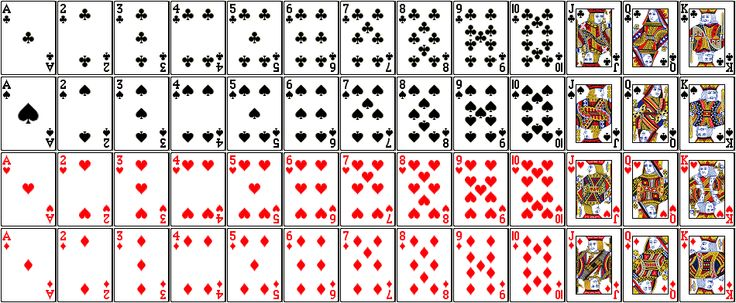
\includegraphics[width=10cm]{./pe/deck.jpg}
	\caption{Baraja inglesa}
	\label{fig:fundamentos-deck}
\end{figure}

\subsection*{Enunciados de los problemas}

% Recordar
\begin{problema}
	\label{prob:de3947a}
	Una carta se obtiene al azar de una baraja inglesa de 52 cartas. Describe formalmente el espacio muestral $S$ si se consideran los palos y los rangos.
\end{problema}

% Comprender
\begin{problema}
	\label{prob:cfa53ca}
	Supongamos que $A$ es el evento \texttt{``se obtiene un rey''} o simplemente $\set{K},$ mientras que $B$ es el evento \texttt{``se obtiene un tr\'ebol''} o simplemente $\set{\clubsuit}$. Describe con palabras el significado de los siguientes eventos combinados:
	\begin{enumerate}
		\item $A\cup B$
		\item $A\cap B$
		\item $A \cup B'$
		\item $A' \cup B'$
		\item $A - B$
		\item $A'-B'$
		\item $(A\cap B) \cup (A\cap B')$
	\end{enumerate}
\end{problema}

% Aplicar
\begin{problema}
	\label{prob:69a20ec}
	Encuéntrese la probabilidad exacta de que en dos lanzamientos de un dado balanceado de 6 caras se obtenga por lo menos un 4 en alguno de los dos lanzamientos.
\end{problema}

% Analizar
\begin{problema}
	\label{prob:1f335a1}
	A partir exclusivamente de los tres axiomas de Kolmogorov ($P(A) \ge 0$, $P(S)=1$, y aditividad para eventos mutuamente excluyentes), demuestra la regla general de adición para dos eventos arbitrarios $A, B \subset S$:
	\begin{align}
		P(A \cup B) = P(A) + P(B) - P(A \cap B).
	\end{align}
\end{problema}

% Evaluar
\begin{problema}
	\label{prob:a4ff50c}
	En una cena de gala, $n$ invitados dejan sus sombreros en el guardarropa. Al finalizar la velada, el encargado devuelve los $n$ sombreros de manera completamente aleatoria. Sea $A_{i}$ el evento de que el $i$-ésimo invitado reciba su propio sombrero ($i=1,2,\dots,n$).
	\begin{enumerate}
		\item Utilizando el principio de inclusión-exclusión para probabilidades, evalúa y demuestra la fórmula general para la probabilidad de que \emph{al menos uno} de los invitados reciba su sombrero correcto:
		\begin{align}
			P\left( \bigcup_{i=1}^{n} A_{i} \right) = \sum_{k=1}^{n} \frac{(-1)^{k-1}}{k!}.
		\end{align}
		\item Calcule el límite de esta probabilidad cuando el número de invitados crece indefinidamente ($n \to \infty$) y juzgue por qué el resultado es contraintuitivo.
	\end{enumerate}
\end{problema}

% Crear
\begin{problema}
	\label{prob:b993271}
	Diseñe un experimento aleatorio original (distinto de cartas, dados o sombreros) con un espacio muestral $S$ de al menos 8 puntos muestrales equiprobables, y defina sobre él dos eventos $A$ y $B$ no disjuntos. Calcule $P(A)$, $P(B)$, $P(A \cap B)$ directamente por conteo, y verifique numéricamente que su resultado satisface la regla general de adición $P(A \cup B) = P(A) + P(B) - P(A \cap B)$.
\end{problema}

\subsection*{Soluciones detalladas}

% Recordar
\begin{solproblema}[prob:de3947a]
	La solución está dada por el producto cartesiano del conjunto de palos:
	\begin{align}
		P = \set{\spadesuit, \heartsuit, \diamondsuit, \clubsuit},
	\end{align}
	cuya cardinalidad es 4, y el conjunto de rangos:
	\begin{align}
		R = \set{\text{A}, 2, 3, 4, 5, 6, 7, 8, 9, 10, \text{J}, \text{Q}, \text{K}},
	\end{align}
	cuya cardinalidad es 13. El espacio muestral completo es $S = P \times R$, conteniendo exactamente $4 \times 13 = 52$ puntos muestrales equiprobables.
\end{solproblema}

% Comprender
\begin{solproblema}[prob:cfa53ca]
	\begin{enumerate}
		\item $A \cup B$: Se obtiene un rey o un trébol (o ambos).
		\item $A \cap B$: Se obtiene simultáneamente un rey y un trébol (específicamente, el Rey de Tréboles).
		\item $A \cup B'$: Se obtiene un rey o no se obtiene un trébol (equivalente a: si es trébol, necesariamente es rey).
		\item $A' \cup B'$: No se obtiene un rey o no se obtiene un trébol (por Ley de De Morgan, es el complemento de obtener el Rey de Tréboles).
		\item $A - B$: Se obtiene un rey que no es de trébol ($A \cap B'$).
		\item $A' - B'$: No se obtiene rey y además sí se obtiene trébol ($A' \cap B$).
		\item $(A \cap B) \cup (A \cap B')$: Se obtiene un rey que es de trébol o un rey que no es de trébol. Por distributividad de la intersección respecto a la unión, esto equivale simplemente al evento $A$ (\texttt{``se obtiene un rey''}).
	\end{enumerate}
\end{solproblema}

% Aplicar
\begin{solproblema}[prob:69a20ec]
	El espacio muestral del lanzamiento de dos dados consta de $6 \times 6 = 36$ pares ordenados equiprobables. Calculamos por el evento complementario: el evento $E'$ de \emph{no} obtener ningún 4 en ninguno de los dos dados significa que cada dado puede caer en cualquiera de las 5 caras restantes ($\{1,2,3,5,6\}$).

	El número de casos favorables para el complemento $E'$ es $5 \times 5 = 25$. Por lo tanto, la probabilidad del evento $E$ (\texttt{``al menos un 4''}) es:
	\begin{align}
		P(E) = 1 - P(E') = 1 - \dfrac{25}{36} = \dfrac{11}{36} \approx 0.3056.
	\end{align}
\end{solproblema}

% Analizar
\begin{solproblema}[prob:1f335a1]
	A partir de la teoría de particiones, podemos expresar el conjunto unión $A \cup B$ y el conjunto $B$ como uniones de conjuntos mutuamente excluyentes (disjuntos):
	\begin{align}
		A \cup B &= A \cup (B \backslash A) \\
		B &= (A \cap B) \cup (B \backslash A)
	\end{align}
	Por el tercer axioma de Kolmogorov (aditividad numerable para conjuntos disjuntos):
	\begin{align}
		P(A \cup B) &= P(A) + P(B \backslash A) \label{eq:fundprob_u1} \\
		P(B) &= P(A \cap B) + P(B \backslash A) \implies P(B \backslash A) = P(B) - P(A \cap B) \label{eq:fundprob_u2}
	\end{align}
	Sustituyendo la ecuación (\ref{eq:fundprob_u2}) en la ecuación (\ref{eq:fundprob_u1}):
	\begin{align}
		P(A \cup B) = P(A) + P(B) - P(A \cap B).
	\end{align}
	Esta identidad demuestra la regla general de adición en probabilidad sin depender de conteos finitos.
\end{solproblema}

% Evaluar
\begin{solproblema}[prob:a4ff50c]
	\begin{enumerate}
		\item La probabilidad de que una persona reciba su sombrero correcto es la relación entre permutaciones que fijan al menos un elemento. Para un índice individual $i$, $P(A_i) = \frac{(n-1)!}{n!} = \frac{1}{n}$. Para dos personas $i < j$, $P(A_i \cap A_j) = \frac{(n-2)!}{n!} = \frac{1}{n(n-1)}$. En general, para la intersección de $k$ personas simultáneas, la probabilidad es $\frac{(n-k)!}{n!}$.

		El principio general de inclusión-exclusión para $n$ eventos establece:
		\begin{align}
			P\left( \bigcup_{i=1}^{n} A_i \right) = \sum_{i=1}^n P(A_i) - \sum_{i<j} P(A_i \cap A_j) + \dots + (-1)^{n-1} P(A_1 \cap \dots \cap A_n).
		\end{align}
		El número de formas de elegir $k$ personas de un total de $n$ es $\binom{n}{k}$. Multiplicando la probabilidad conjunta por el número de combinaciones en el término $k$-ésimo:
		\begin{align}
			S_k = \binom{n}{k} \cdot \frac{(n-k)!}{n!} = \frac{n!}{k!(n-k)!} \cdot \frac{(n-k)!}{n!} = \frac{1}{k!}.
		\end{align}
		Sustituyendo cada suma parcial $S_k$ en la fórmula principal:
		\begin{align}
			P\left( \bigcup_{i=1}^{n} A_i \right) = \sum_{k=1}^{n} (-1)^{k-1} S_k = \sum_{k=1}^{n} \frac{(-1)^{k-1}}{k!}.
		\end{align}

		\item Recordemos la serie de Taylor para la función exponencial evaluada en $x = -1$:
		\begin{align}
			e^{-1} = \sum_{k=0}^{\infty} \frac{(-1)^k}{k!} = 1 - \sum_{k=1}^{\infty} \frac{(-1)^{k-1}}{k!}.
		\end{align}
		Por lo tanto, cuando el número de invitados crece ($n \to \infty$):
		\begin{align}
			\lim_{n \to \infty} P\left( \bigcup_{i=1}^{n} A_i \right) = 1 - e^{-1} \approx 0.63212.
		\end{align}
		El resultado es contraintuitivo porque es \emph{independiente del tamaño de la cena}: ya sea con $n=10$ o $n=10{,}000$ invitados, la probabilidad de que al menos uno reciba su propio sombrero se estabiliza de manera prácticamente idéntica en $63.21\%$ a partir de $n \ge 6$, en contra de la intuición de que agregar más invitados debería diluir la probabilidad de una coincidencia.
	\end{enumerate}
\end{solproblema}

% Crear
\begin{solproblema}[prob:b993271]
	\textbf{Ejemplo:} un dado balanceado de 8 caras (numeradas 1 a 8) se lanza una vez, de modo que $S=\{1,2,\dots,8\}$ con $8$ puntos equiprobables. Sea $A=\{2,3,4,5\}$ (\texttt{``el resultado es par o impar entre 2 y 5''}) y $B=\{4,5,6,7\}$ (\texttt{``el resultado está entre 4 y 7''}), que no son disjuntos porque $A\cap B=\{4,5\}$.

	Por conteo directo:
	\begin{align}
		P(A) = \frac{4}{8}=0.5, \qquad P(B) = \frac{4}{8}=0.5, \qquad P(A\cap B) = \frac{2}{8}=0.25.
	\end{align}
	La unión es $A\cup B=\{2,3,4,5,6,7\}$, con $P(A\cup B)=6/8=0.75$ por conteo directo. Verificando con la regla general de adición:
	\begin{align}
		P(A) + P(B) - P(A\cap B) = 0.5+0.5-0.25 = 0.75 = P(A\cup B),
	\end{align}
	confirmando que el conteo directo y la fórmula coinciden exactamente.
\end{solproblema}

\input{probabilidad_condicional}
\section*{Problemas}

\begin{problema}
	\label{prob-cond-1}
	Se lanzan dos dados. Sea $A$ el evento de que la suma sea al menos 9, y sea $B$ el evento de que el primer dado muestre un número par.
	\begin{enumerate}
		\item Calcula $P(A)$
		\item Calcula $P(B)$
		\item Calcula $P(A|B)$
		\item ¿Son $A$ y $B$ independientes?
	\end{enumerate}
\end{problema}

\begin{solucion}
	El espacio muestral tiene $6 \times 6 = 36$ resultados.
	
	\begin{enumerate}
		\item $A = \{(3,6), (4,5), (4,6), (5,4), (5,5), (5,6), (6,3), (6,4), (6,5), (6,6)\}$, entonces $\card{A} = 10$ y $P(A) = \frac{10}{36} = \frac{5}{18}$.
		
		\item $B$ = primer dado es par = $\{2,4,6\} \times \{1,2,3,4,5,6\}$, entonces $\card{B} = 18$ y $P(B) = \frac{18}{36} = \frac{1}{2}$.
		
		\item $A \cap B = \{(4,5), (4,6), (6,3), (6,4), (6,5), (6,6)\}$, entonces $\card{A \cap B} = 6$ y
		\begin{align}
			P(A|B) = \frac{P(A \cap B)}{P(B)} = \frac{6/36}{18/36} = \frac{6}{18} = \frac{1}{3}
		\end{align}
		
		\item Como $P(A|B) = \frac{1}{3} \neq \frac{5}{18} = P(A)$, los eventos \textbf{no son independientes}.
	\end{enumerate}
\end{solucion}

\begin{problema}
	\label{prob-cond-2}
	Una urna contiene 5 bolas rojas y 3 bolas azules. Se extraen dos bolas sucesivamente sin reemplazo. Sea $A$ = ``la primera bola es roja'' y $B$ = ``la segunda bola es roja''.
	\begin{enumerate}
		\item Calcula $P(A)$
		\item Calcula $P(B|A)$
		\item Calcula $P(B|A')$
		\item Calcula $P(B)$ usando la regla de la probabilidad total
	\end{enumerate}
\end{problema}

\begin{solucion}
	\begin{enumerate}
		\item $P(A) = \frac{5}{8}$
		
		\item Si la primera es roja, quedan 4 rojas y 3 azules (7 bolas en total):
		\begin{align}
			P(B|A) = \frac{4}{7}
		\end{align}
		
		\item Si la primera es azul, quedan 5 rojas y 2 azules (7 bolas en total):
		\begin{align}
			P(B|A') = \frac{5}{7}
		\end{align}
		
		\item Por la regla de la probabilidad total:
		\begin{align}
			P(B) &= P(B|A)P(A) + P(B|A')P(A') \\
			&= \frac{4}{7} \cdot \frac{5}{8} + \frac{5}{7} \cdot \frac{3}{8} \\
			&= \frac{20}{56} + \frac{15}{56} = \frac{35}{56} = \frac{5}{8}
		\end{align}
	\end{enumerate}
\end{solucion}

\begin{problema}
	\label{prob-cond-3}
	En una fábrica, el 70\% de las piezas son producidas por la máquina A y el 30\% por la máquina B. La máquina A tiene una tasa de defectos del 5\%, mientras que la máquina B tiene una tasa de defectos del 10\%. Si se elige una pieza al azar:
	\begin{enumerate}
		\item ¿Cuál es la probabilidad de que la pieza sea defectuosa?
		\item Si la pieza es defectuosa, ¿cuál es la probabilidad de que provenga de la máquina A?
	\end{enumerate}
\end{problema}

\begin{solucion}
	Sea $D$ = ``la pieza es defectuosa'', $A$ = ``proviene de la máquina A'', $B$ = ``proviene de la máquina B''.
	
	\begin{enumerate}
		\item Por la regla de la probabilidad total:
		\begin{align}
			P(D) &= P(D|A)P(A) + P(D|B)P(B) \\
			&= 0.05 \times 0.70 + 0.10 \times 0.30 \\
			&= 0.035 + 0.03 = 0.065
		\end{align}
		
		\item Por el teorema de Bayes:
		\begin{align}
			P(A|D) &= \frac{P(D|A)P(A)}{P(D)} \\
			&= \frac{0.05 \times 0.70}{0.065} = \frac{0.035}{0.065} \approx 0.538
		\end{align}
	\end{enumerate}
\end{solucion}

\begin{problema}
	\label{prob-cond-4}
	Se sabe que el 80\% de los estudiantes de una universidad aprueban el examen de cálculo. De los que aprueban, el 90\% asistió a clases regularmente. De los que no aprueban, solo el 40\% asistió regularmente.
	\begin{enumerate}
		\item Si un estudiante aprobó el examen, ¿cuál es la probabilidad de que haya asistido regularmente?
		\item Si un estudiante no asistió regularmente, ¿cuál es la probabilidad de que haya aprobado?
	\end{enumerate}
\end{problema}

\begin{solucion}
	Sea $A$ = ``aprobó'', $R$ = ``asistió regularmente'', $A'$ = ``no aprobó''.
	
	\begin{enumerate}
		\item Por la regla de la probabilidad total:
		\begin{align}
			P(R|A) &= \frac{P(A|R)P(R)}{P(A)}
		\end{align}
		
		Necesitamos calcular $P(A)$:
		\begin{align}
			P(A) &= P(A|R)P(R) + P(A|R')P(R') \\
			&= 0.90 \times 0.80 + 0.40 \times 0.20 \\
			&= 0.72 + 0.08 = 0.80
		\end{align}
		
		Entonces:
		\begin{align}
			P(R|A) &= \frac{0.90 \times 0.80}{0.80} = \frac{0.72}{0.80} = 0.90
		\end{align}
		
		\item Si no asistió regularmente ($A'$), entonces $R'$:
		\begin{align}
			P(A) &= P(A|R')P(R') + P(A|R)P(R) \\
			&= 0.40 \times 0.20 + 0.90 \times 0.80 \\
			&= 0.08 + 0.72 = 0.80
		\end{align}
		
		Y por Bayes:
		\begin{align}
			P(R|A') &= \frac{P(A|R')P(R')}{P(A)} \\
			&= \frac{0.40 \times 0.20}{0.80} = \frac{0.08}{0.80} = 0.10
		\end{align}
	\end{enumerate}
\end{solucion}

\begin{problema}
	\label{prob-cond-5}
	Un fabricante produce dos tipos de piezas: tipo A con probabilidad 0.6 y tipo B con probabilidad 0.4. Las piezas tipo A tienen una tasa de defectos del 2\%, mientras que las tipo B tienen una tasa de defectos del 5\%. Si se selecciona una pieza al azar y resulta defectuosa, ¿cuál es la probabilidad de que sea tipo A?
\end{problema}

\begin{solucion}
	Sea $D$ = ``pieza defectuosa'', $A$ = ``tipo A'', $B$ = ``tipo B''.
	
	\begin{enumerate}
		\item Por la regla de la probabilidad total:
		\begin{align}
			P(D) &= P(D|A)P(A) + P(D|B)P(B) \\
			&= 0.02 \times 0.6 + 0.05 \times 0.4 \\
			&= 0.012 + 0.020 = 0.032
		\end{align}
		
		\item Por el teorema de Bayes:
		\begin{align}
			P(A|D) &= \frac{P(D|A)P(A)}{P(D)} \\
			&= \frac{0.02 \times 0.6}{0.032} = \frac{0.012}{0.032} = 0.375
		\end{align}
	\end{enumerate}
\end{solucion}

\begin{problema}
	\label{prob-cond-6}
	Demuestra que si $P(B|A) = P(B)$, entonces $A$ y $B$ son independientes.
\end{problema}

\begin{solucion}
	Si $P(B|A) = P(B)$, por definición de probabilidad condicional:
	\begin{align}
		P(B|A) &= \frac{P(A \cap B)}{P(A)} = P(B) \\
		\Rightarrow P(A \cap B) &= P(A)P(B)
	\end{align}
	
	que es precisamente la definición de independencia.
\end{solucion}

\input{teorema_de_bayes}
\section*{Problemas}

\subsection*{Enunciados de los problemas}

% Recordar
\begin{problema}
	\label{prob:054ed26}
	Encontrar la probabilidad de que un solo lanzamiento de un dado balanceado de 6 caras resulte en un número menor que 4 si:
	\begin{enumerate}
		\item no hay más información disponible;
		\item se sabe con certeza que el lanzamiento resultó en un número impar.
	\end{enumerate}
\end{problema}

% Comprender
\begin{problema}
	\label{prob:bde7784}
	En un grupo de estudiantes de estadística, el 60\% son mujeres ($M$) y el 40\% son hombres ($H$). Se sabe que el 10\% de las mujeres son zurdas ($Z$) y el 15\% de los hombres son zurdos. Si se selecciona una persona al azar y resulta ser zurda, calcula aplicando el Teorema de Bayes la probabilidad de que sea mujer, y explica por qué este resultado no es simplemente igual a la proporción original de mujeres en el grupo ($60\%$).
\end{problema}

% Aplicar
\begin{problema}
	\label{prob:e14faa0}
	Un estudiante se prepara para un examen general. Si estudia debidamente ($E$), la probabilidad de aprobar ($A$) es de 0.90. Si no estudia ($E'$), la probabilidad de aprobar es de sólo 0.30. La probabilidad de que el estudiante estudie es de 0.70.
	\begin{enumerate}
		\item ¿Cuál es la probabilidad total de que el estudiante apruebe el examen?
		\item Si el estudiante aprobó, ¿cuál es la probabilidad condicional de que haya estudiado?
		\item Si el estudiante no aprobó, ¿cuál es la probabilidad de que no haya estudiado?
	\end{enumerate}
\end{problema}

% Analizar
\begin{problema}
	\label{prob:a7e87e4}
	Demuestra rigurosamente el Teorema de Bayes para una partición finita y exhaustiva $\{B_1, B_2, \dots, B_k\}$ del espacio muestral $S$ dado un evento observable $A$ con $P(A)>0$:
	\begin{align}
		P(B_j | A) = \frac{P(A|B_j)P(B_j)}{\sum_{i=1}^k P(A|B_i)P(B_i)}, \quad \text{para todo } j \in \{1, \dots, k\}.
	\end{align}
\end{problema}

% Evaluar
\begin{problema}
	\label{prob:898898e}
	\textbf{La Falacia del Fiscal y la razón de momios:} En una investigación forense se recupera una muestra biológica en la escena del crimen. El perfil de ADN extraído tiene una probabilidad de coincidencia aleatoria en la población de $\alpha = 10^{-6}$ (es decir, $P(\text{coincidencia} | \text{inocente}) = 10^{-6}$). Un sospechoso es identificado mediante un rastreo masivo y su ADN coincide perfectamente con la muestra ($P(\text{coincidencia} | \text{culpable}) = 1$). El fiscal afirma ante el jurado que, puesto que la probabilidad de coincidencia aleatoria es de apenas una en un millón, la probabilidad de que el sospechoso sea inocente es del $0.0001\%$.

	Evalúa mediante la formulación en momios (odds ratio) del Teorema de Bayes por qué el razonamiento del fiscal es erróneo. Si en la región habitan $N = 5,000,000$ de personas con posible acceso a la escena y no existe ninguna otra evidencia contra el sospechoso, calcula la verdadera probabilidad a posteriori de culpabilidad $P(\text{culpable} | \text{coincidencia})$.
\end{problema}

% Crear
\begin{problema}
	\label{prob:3bf9f42}
	Diseñe un problema original de clasificación de riesgo crediticio: un banco clasifica a sus solicitantes de préstamo en tres categorías de historial —Excelente, Regular y Deficiente— que representan el $50\%$, $35\%$ y $15\%$ de los solicitantes, respectivamente. Las tasas históricas de incumplimiento (\emph{default}) son del $2\%$, $8\%$ y $25\%$ en cada categoría. Calcule el vector completo de probabilidades a posteriori dado que un préstamo entró en incumplimiento, e identifique cuál categoría es la fuente más probable de incumplimientos en términos absolutos, a pesar de no ser la más numerosa.
\end{problema}

\subsection*{Soluciones detalladas}

% Recordar
\begin{solproblema}[prob:054ed26]
	\begin{enumerate}
		\item \textbf{Sin información:} el espacio muestral completo tiene 6 eventos equiprobables $S=\{1,2,3,4,5,6\}$. Los resultados estrictamente menores que 4 son $A=\{1,2,3\}$, por lo que $P(A) = \frac{3}{6} = 0.50$.
		\item \textbf{Con información de número impar:} el espacio condicionado es $I=\{1,3,5\}$. Los elementos de $A$ que también están en $I$ son $A \cap I = \{1,3\}$. Aplicando la definición de probabilidad condicional:
		\begin{align}
			P(A|I) = \frac{P(A \cap I)}{P(I)} = \frac{2/6}{3/6} = \frac{2}{3} \approx 0.6667.
		\end{align}
	\end{enumerate}
\end{solproblema}

% Comprender
\begin{solproblema}[prob:bde7784]
	Sean los eventos $M$ (mujer) con $P(M)=0.60$ y $H$ (hombre) con $P(H)=0.40$. Las tasas de zurdería son $P(Z|M)=0.10$ y $P(Z|H)=0.15$.

	Por la regla de la probabilidad total, la probabilidad de que una persona elegida al azar sea zurda es:
	\begin{align}
		P(Z) = P(Z|M)P(M) + P(Z|H)P(H) = (0.10)(0.60) + (0.15)(0.40) = 0.060 + 0.060 = 0.120.
	\end{align}
	Por el Teorema de Bayes:
	\begin{align}
		P(M|Z) = \frac{P(Z|M)P(M)}{P(Z)} = \frac{0.060}{0.120} = 0.50 \text{ (50\%).}
	\end{align}
	Este resultado ($50\%$) es menor que la proporción original de mujeres en el grupo ($60\%$) porque \emph{observar que la persona es zurda} es evidencia que favorece relativamente más a los hombres: aunque hay más mujeres en total, los hombres tienen una tasa de zurdería más alta ($15\%$ contra $10\%$), así que condicionar sobre "ser zurdo" desplaza la probabilidad hacia el grupo con mayor propensión relativa a ese rasgo, no solo hacia el grupo más numeroso.
\end{solproblema}

% Aplicar
\begin{solproblema}[prob:e14faa0]
	Sea $A$ el evento de aprobar y $E$ el de estudiar ($P(E)=0.70$, $P(E')=0.30$). Las probabilidades condicionales del examen son $P(A|E)=0.90$ y $P(A|E')=0.30$.
	\begin{enumerate}
		\item Probabilidad marginal total de aprobar:
		\begin{align}
			P(A) = P(A|E)P(E) + P(A|E')P(E') = (0.90)(0.70) + (0.30)(0.30) = 0.63 + 0.09 = 0.72 \text{ (72\%).}
		\end{align}
		\item Por el Teorema de Bayes, si aprobó, la probabilidad de haber estudiado es:
		\begin{align}
			P(E|A) = \frac{P(A|E)P(E)}{P(A)} = \frac{0.63}{0.72} = 0.875 \text{ (87.5\%).}
		\end{align}
		\item Para $A'$: $P(A') = 1-0.72=0.28$; $P(A'|E)=0.10$, $P(A'|E')=0.70$. Por Bayes sobre los complementos:
		\begin{align}
			P(E'|A') = \frac{P(A'|E')P(E')}{P(A')} = \frac{(0.70)(0.30)}{0.28} = \frac{0.21}{0.28} = 0.75 \text{ (75\%).}
		\end{align}
	\end{enumerate}
\end{solproblema}

% Analizar
\begin{solproblema}[prob:a7e87e4]
	Sea $\{B_1, B_2, \dots, B_k\}$ una partición exhaustiva ($\bigcup_{i=1}^k B_i = S$) y mutuamente excluyente. Por la regla del producto de la probabilidad condicional, para cualquier índice $j$:
	\begin{align}
		P(B_j \cap A) = P(B_j | A) P(A) = P(A | B_j) P(B_j).
	\end{align}
	Al despejar $P(B_j|A)$ dado que $P(A)>0$:
	\begin{align}
		P(B_j | A) = \frac{P(A | B_j) P(B_j)}{P(A)}. \label{eq:bayes_num_tdb}
	\end{align}
	Como los eventos $B_i$ forman una partición de $S$, expresamos $A$ como la unión disjunta de sus intersecciones sobre cada celda:
	\begin{align}
		A = A \cap S = A \cap \left( \bigcup_{i=1}^k B_i \right) = \bigcup_{i=1}^k (A \cap B_i).
	\end{align}
	Por el tercer axioma de Kolmogorov (aditividad para eventos disjuntos):
	\begin{align}
		P(A) = \sum_{i=1}^k P(A \cap B_i) = \sum_{i=1}^k P(A | B_i) P(B_i). \label{eq:prob_total_k_tdb}
	\end{align}
	Sustituyendo (\ref{eq:prob_total_k_tdb}) en (\ref{eq:bayes_num_tdb}), se obtiene la fórmula general del Teorema de Bayes para $k$ estados.
\end{solproblema}

% Evaluar
\begin{solproblema}[prob:898898e]
	Sea $I$ el evento de ser el culpable real del crimen, y $E$ la coincidencia en el perfil de ADN. El fiscal incurre en una falacia condicional al igualar erróneamente $P(E|I') = 10^{-6}$ con la probabilidad inversa $P(I'|E)$.

	Evaluamos la veracidad formal mediante la versión del Teorema de Bayes en razón de momios (Odds Form):
	\begin{align}
		\frac{P(I|E)}{P(I'|E)} = \underbrace{\frac{P(E|I)}{P(E|I')}}_{\text{Likelihood Ratio (LR)}} \times \underbrace{\frac{P(I)}{P(I')}}_{\text{Momios a priori}}.
	\end{align}
	Sin más evidencias que la ubicación geográfica en la población de $N = 5,000,000$ habitantes, la probabilidad a priori de que un individuo arbitrario sea culpable es $P(I) = \frac{1}{5,000,000} = 2 \times 10^{-7}$, con $P(I') \approx 1$. El cociente de verosimilitud es:
	\begin{align}
		\text{LR} = \frac{P(E|I)}{P(E|I')} = \frac{1}{10^{-6}} = 1,000,000.
	\end{align}
	Los momios a posteriori son:
	\begin{align}
		\text{Momios}(I|E) = 1,000,000 \times \frac{1/5,000,000}{1} = \frac{1}{5} = 0.20.
	\end{align}
	Convirtiendo a probabilidad exacta:
	\begin{align}
		P(I|E) = \frac{0.20}{1+0.20} = \frac{1}{6} \approx 0.1667 \text{ (16.67\%).}
	\end{align}
	La probabilidad de que el sospechoso sea culpable es de sólo $16.67\%$ (no del $99.9999\%$ como alegaba el fiscal). El error radica en no considerar que, al evaluar un perfil en una población de 5 millones donde la frecuencia de coincidencia aleatoria es 1 en 1 millón, se esperan estadísticamente unos 5 falsos positivos puramente aleatorios en la población —el sospechoso es apenas uno entre esos 5 candidatos igualmente compatibles, más el verdadero culpable.
\end{solproblema}

% Crear
\begin{solproblema}[prob:3bf9f42]
	Sean las categorías $Exc$, $Reg$, $Def$ con $P(Exc)=0.50$, $P(Reg)=0.35$, $P(Def)=0.15$, y tasas de incumplimiento $P(D|Exc)=0.02$, $P(D|Reg)=0.08$, $P(D|Def)=0.25$.

	La probabilidad marginal de incumplimiento es:
	\begin{align}
		P(D) = (0.02)(0.50)+(0.08)(0.35)+(0.25)(0.15) = 0.010+0.028+0.0375 = 0.0755.
	\end{align}
	El vector de probabilidades a posteriori es:
	\begin{align}
		P(Exc|D) &= \frac{0.010}{0.0755} \approx 0.1325 \text{ (13.25\%)} \\
		P(Reg|D) &= \frac{0.028}{0.0755} \approx 0.3709 \text{ (37.09\%)} \\
		P(Def|D) &= \frac{0.0375}{0.0755} \approx 0.4967 \text{ (49.67\%)}
	\end{align}
	La categoría \textbf{Deficiente} es la fuente más probable de incumplimientos en términos absolutos ($49.67\%$), a pesar de representar apenas el $15\%$ de los solicitantes: su tasa de incumplimiento ($25\%$) es tan desproporcionadamente alta que domina el cálculo, de forma análoga a como una línea de producción pequeña pero muy defectuosa puede superar en piezas defectuosas absolutas a una línea grande pero confiable.
\end{solproblema}

\section{Muestreo aleatorio}

\subsection{Motivación: Estimación de parámetros poblacionales}

Supongamos que tratamos de encontrar la edad promedio en una ciudad, digamos Oaxaca. Una manera de hacerlo sería por \emph{fuerza bruta}, es decir, recolectando esta información persona por persona. Pero este método sería muy costoso en términos de infraestructura y tiempo.

En estadística, este es un problema común, cuya solución está en el \emph{muestreo aleatorio}: Tomemos un grupo de 1000 individuos (o 10,000 dependiendo de tu capacidad, obviamente entre más, es mejor) y calculemos la edad promedio en este grupo, a la que denotaremos por $A_{1}.$

Repitamos este procedimiento, digamos 100 veces, y denotaremos por $A_{1}, A_{2},...,A_{100}$ el promedio de edades obtenido en cada respectivo intento.

\subsection{Ley de los grandes números}

De acuerdo a la \emph{ley de los grandes números}, la cantidad
\begin{align}
	\bar{A}_{100}=\dfrac{A_{1}+...+A_{100}}{100}
\end{align}
es una aproximación muy cercana al promedio real de la edad de los pobladores de la ciudad.

\begin{observacion}
	No estamos más interesados en obtener el valor exacto de la edad promedio, sino establecer un \emph{estimador} para la misma. En tal caso, tenemos que conformarnos con la definición de un \emph{rango de valores} en el que el valor real podría estar.
\end{observacion}

\subsection{Teorema del límite central}

De acuerdo al \emph{teorema del límite central}, si el número de tales muestras es suficientemente grande, $A_{1},A_{2},...,A_{100}$ estarán distribuidos de manera normal.

\begin{teorema}[Teorema del límite central]
	Si $X_1, X_2, \ldots, X_n$ son variables aleatorias independientes e idénticamente distribuidas con media $\mu$ y varianza $\sigma^2$, entonces cuando $n$ es suficientemente grande:
	\begin{align}
		\frac{\bar{X} - \mu}{\sigma/\sqrt{n}} \xrightarrow{d} N(0,1)
	\end{align}
	
	Es decir, la distribución de la media muestral estandarizada se aproxima a una distribución normal estándar.
\end{teorema}

\subsection{Implicaciones prácticas del TLC}

El teorema del límite central tiene profundas implicaciones para la inferencia estadística:

\begin{enumerate}
	\item \textbf{Independencia de la distribución original:} No importa si la población original sigue una distribución normal, exponencial, uniforme o cualquier otra. La distribución de la media muestral será aproximadamente normal para muestras grandes.
	
	\item \textbf{Tamaño de muestra:} En la práctica, $n \geq 30$ suele ser suficiente para que la aproximación normal sea buena, aunque esto depende de la forma de la distribución original.
	
	\item \textbf{Parámetros de la distribución muestral:}
	\begin{align}
		E(\bar{X}) &= \mu \\
		\text{Var}(\bar{X}) &= \frac{\sigma^2}{n} \\
		\text{DE}(\bar{X}) &= \frac{\sigma}{\sqrt{n}}
	\end{align}
\end{enumerate}

\subsection{Ejemplo ilustrativo}

Consideremos el lanzamiento de un dado justo. La distribución de un solo lanzamiento es uniforme discreta en $\{1, 2, 3, 4, 5, 6\}$ con:
\begin{align}
	\mu &= \frac{1+2+3+4+5+6}{6} = 3.5 \\
	\sigma^2 &= \frac{(1-3.5)^2 + (2-3.5)^2 + \cdots + (6-3.5)^2}{6} = \frac{35}{12} \approx 2.917
\end{align}

Si lanzamos el dado $n = 36$ veces y calculamos el promedio $\bar{X}$, por el TLC:
\begin{align}
	\bar{X} \sim N\left(3.5, \frac{2.917}{36}\right) = N(3.5, 0.081)
\end{align}

Esto significa que:
\begin{align}
	P(3.0 < \bar{X} < 4.0) &= P\left(\frac{3.0-3.5}{\sqrt{0.081}} < Z < \frac{4.0-3.5}{\sqrt{0.081}}\right) \\
	&= P(-1.76 < Z < 1.76) \\
	&\approx 0.921
\end{align}

Hay aproximadamente un 92.1\% de probabilidad de que el promedio de 36 lanzamientos esté entre 3.0 y 4.0.

\subsection{Simulación del TLC con Python}

Podemos verificar el teorema del límite central mediante simulación:

\begin{lstlisting}[language=Python]
import numpy as np
import matplotlib.pyplot as plt

# Parámetros
n = 30  # tamaño de muestra
num_simulaciones = 10000

# Simulación: promedio de n valores de una distribución exponencial
medias_muestrales = []
for _ in range(num_simulaciones):
    muestra = np.random.exponential(scale=2.0, size=n)
    medias_muestrales.append(np.mean(muestra))

# Graficar histograma
plt.hist(medias_muestrales, bins=50, density=True, alpha=0.7)

# Superponer curva normal teórica
mu = 2.0  # media de la exponencial
sigma = 2.0  # desviación estándar de la exponencial
x = np.linspace(mu - 4*sigma/np.sqrt(n), mu + 4*sigma/np.sqrt(n), 100)
y = (1/(sigma/np.sqrt(n) * np.sqrt(2*np.pi))) * np.exp(-0.5*((x-mu)/(sigma/np.sqrt(n)))**2)
plt.plot(x, y, 'r-', linewidth=2)

plt.xlabel('Media muestral')
plt.ylabel('Densidad')
plt.title(f'Distribución de medias muestrales (n={n})')
plt.show()
\end{lstlisting}

\subsection{Aplicaciones del TLC}

El teorema del límite central es fundamental en muchas áreas:

\begin{itemize}
	\item \textbf{Control de calidad:} Las medias de mediciones de calidad siguen distribuciones normales, permitiendo el uso de gráficos de control.
	
	\item \textbf{Encuestas y sondeos:} Las proporciones muestrales (que son promedios de variables binarias) siguen distribuciones normales aproximadas.
	
	\item \textbf{Finanzas:} Los rendimientos promedio de carteras de inversión se modelan como normales.
	
	\item \textbf{Ciencias naturales:} Muchas mediciones biológicas y físicas son el resultado de muchos factores pequeños e independientes, por lo que siguen distribuciones normales.
\end{itemize}

\subsection{Limitaciones y consideraciones}

Aunque el TLC es muy poderoso, es importante recordar:

\begin{enumerate}
	\item \textbf{Tamaño de muestra:} Para distribuciones muy asimétricas o con colas pesadas, puede requerirse $n > 30$ para una buena aproximación.
	
	\item \textbf{Independencia:} Las observaciones deben ser independientes. Si hay correlación entre observaciones, el TLC puede no aplicarse.
	
	\item \textbf{Varianza finita:} El TLC requiere que la varianza poblacional sea finita. Para distribuciones con varianza infinita (como la distribución de Cauchy), el TLC no se aplica.
\end{enumerate}

\subsection{Resumen}

El muestreo aleatorio y el teorema del límite central son la columna vertebral de la inferencia estadística:

\begin{itemize}
	\item El \textbf{muestreo aleatorio} nos permite hacer inferencias sobre poblaciones grandes a partir de muestras pequeñas.
	
	\item La \textbf{ley de los grandes números} garantiza que nuestras estimaciones convergen a los valores verdaderos.
	
	\item El \textbf{teorema del límite central} nos permite usar la distribución normal para hacer inferencias, incluso cuando la población original no es normal.
\end{itemize}

Estos resultados teóricos justifican las técnicas de estimación y pruebas de hipótesis que estudiaremos en las siguientes secciones.

\section*{Problemas}

\subsection*{Enunciados de los problemas}

% Recordar
\begin{problema}
	\label{prob:c0cebb4}
	El tiempo de ensamblaje de un componente mecánico sigue una distribución con media poblacional $\mu = 45$ minutos y desviación estándar $\sigma = 12$ minutos. Si se toma una muestra aleatoria de tamaño $n$, calcula el error estándar de la media muestral, denotado por $\text{DE}(\bar{X}) = \sigma_{\bar{X}}$, para cada uno de los siguientes tamaños de muestra y comenta sobre la velocidad de reducción del error:
	\begin{enumerate}
		\item $n = 9$
		\item $n = 36$
		\item $n = 144$
		\item $n = 576$
	\end{enumerate}
\end{problema}

% Comprender
\begin{problema}
	\label{prob:116017b}
	Una población finita consta de $N = 6$ elementos distintos $\{a, b, c, d, e, f\}$. Se desea extraer una muestra aleatoria de tamaño $n = 3$.
	\begin{enumerate}
		\item Determina el número total de muestras posibles si la extracción se realiza \textbf{con reemplazo}.
		\item Determina el número total de muestras posibles si la extracción se realiza \textbf{sin reemplazo} y sin importar el orden (muestras no ordenadas).
		\item Explica formalmente por qué, a medida que el tamaño poblacional $N$ crece hacia el infinito, la diferencia probabilística entre muestreo con y sin reemplazo tiende a cero.
	\end{enumerate}
\end{problema}

% Aplicar
\begin{problema}
	\label{prob:2da8cc3}
	Una embotelladora de agua mineral desea calibrar su línea de producción. La cantidad vertida en cada botella es una variable aleatoria con desviación estándar conocida de $\sigma = 8$ mililitros. ¿Cuál es el tamaño de muestra mínimo $n$ que un ingeniero de calidad debe inspeccionar para tener una certeza probabilística de al menos $95\%$ de que la media muestral $\bar{X}$ no difiera de la verdadera media poblacional de llenado $\mu$ en más de $1.5$ mililitros?
\end{problema}

% Analizar
\begin{problema}
	\label{prob:0c980d4}
	Demuestra algebraicamente por qué el estimador de la varianza muestral requiere dividir entre $n-1$ (y no entre $n$) para ser insesgado. Sea $S^2 = \frac{1}{n-1} \sum_{i=1}^n (X_i - \bar{X})^2$ la varianza muestral de una MAS obtenida de una población con media $\mu$ y varianza $\sigma^2$. Demuestra paso a paso que $E(S^2) = \sigma^2$.
	\emph{Sugerencia:} Suma y resta $\mu$ dentro del término cuadrático $(X_i - \bar{X})^2 = [(X_i - \mu) - (\bar{X} - \mu)]^2$.
\end{problema}

% Evaluar
\begin{problema}
	\label{prob:293fd20}
	El Teorema del Límite Central postula que la suma de variables independientes convergerá a la distribución normal siempre que el momento de segundo orden ($\sigma^2$) sea finito. Evalúa qué sucede cuando se extraen muestras de una población con colas extremadamente pesadas: la distribución de Cauchy estándar, cuya densidad es $f(x) = \frac{1}{\pi(1+x^2)}$ para $x \in (-\infty, \infty)$.
	\begin{enumerate}
		\item Demuestra o argumenta formalmente por qué la integral que define la esperanza teórica $E(X)$ no converge absolutamente en la distribución de Cauchy.
		\item Si se extrae una muestra aleatoria de tamaño $n$ de una población Cauchy, ¿cuál es la función de densidad o comportamiento de la media muestral $\bar{X}_n$? ¿Ocurre convergencia hacia la normal conforme $n \to \infty$? Juzga qué implicación práctica tiene esto para un analista que asuma ciegamente el TLC en cualquier conjunto de datos.
	\end{enumerate}
\end{problema}

% Crear
\begin{problema}
	\label{prob:b7567ec}
	Diseñe un problema original de aplicación del Teorema del Límite Central: elija una población con media y varianza poblacional conocidas (distinta del dado o la embotelladora ya vistos en esta sección), un tamaño de muestra $n \ge 30$, y calcule la probabilidad de que la media muestral se encuentre dentro de un rango específico que usted defina.
\end{problema}

\subsection*{Soluciones detalladas}

% Recordar
\begin{solproblema}[prob:c0cebb4]
	El error estándar de la media ($\sigma_{\bar{X}}$) mide la dispersión de los promedios muestrales alrededor de $\mu$ y está dado por $\sigma_{\bar{X}} = \frac{\sigma}{\sqrt{n}}$. Con $\sigma = 12$:
	\begin{enumerate}
		\item Para $n = 9$: $\sigma_{\bar{X}} = \frac{12}{\sqrt{9}} = 4.00$ min.
		\item Para $n = 36$: $\sigma_{\bar{X}} = \frac{12}{\sqrt{36}} = 2.00$ min.
		\item Para $n = 144$: $\sigma_{\bar{X}} = \frac{12}{\sqrt{144}} = 1.00$ min.
		\item Para $n = 576$: $\sigma_{\bar{X}} = \frac{12}{\sqrt{576}} = 0.50$ min.
	\end{enumerate}
	\textbf{Comentario sobre la velocidad de reducción:} la dispersión decrece de manera estrictamente inversamente proporcional a la raíz cuadrada del tamaño muestral ($\sqrt{n}$). Para reducir el error estándar a la mitad (por ejemplo, de 4.0 a 2.0, o de 2.0 a 1.0), es obligatorio cuadruplicar el tamaño de la muestra inspeccionada ($9 \to 36 \to 144$).
\end{solproblema}

% Comprender
\begin{solproblema}[prob:116017b]
	\begin{enumerate}
		\item \textbf{Muestreo con reemplazo:} en cada una de las $n = 3$ extracciones hay exactamente $N = 6$ opciones disponibles, dado que el elemento extraído se devuelve a la población antes de la siguiente selección. Por el principio multiplicativo del conteo:
		\begin{align}
			N^n = 6^3 = 216 \text{ muestras.}
		\end{align}
		\item \textbf{Muestreo sin reemplazo (no ordenado):} el número total de subconjuntos posibles es el coeficiente binomial:
		\begin{align}
			\binom{N}{n} = \binom{6}{3} = \frac{6!}{3!(6-3)!} = 20 \text{ muestras.}
		\end{align}
		\item \textbf{Equivalencia asintótica cuando $N \to \infty$:} al extraer una muestra fija $n$ sin reemplazo, la probabilidad de seleccionar un elemento específico en la primera extracción es $1/N$, en la segunda es $1/(N-1)$, y en la $k$-ésima es $1/(N-k+1)$. A medida que $N \to \infty$ con $n$ constante, las razones $\frac{N-k}{N} \to 1$. Por lo tanto, el agotamiento poblacional es despreciable y el muestreo sin reemplazo converge en distribución al muestreo con reemplazo (independiente).
	\end{enumerate}
\end{solproblema}

% Aplicar
\begin{solproblema}[prob:2da8cc3]
	Datos: $\sigma = 8$ ml, margen de error máximo tolerado $E = 1.5$ ml, nivel de confianza del $95\%$ ($\alpha = 0.05$, $z_{\alpha/2}=1.96$). El margen de error de estimación de la media es $E = z_{\alpha/2} \cdot \sigma/\sqrt{n}$. Despejando el tamaño de muestra mínimo:
	\begin{align}
		n = \left( \frac{z_{\alpha/2} \cdot \sigma}{E} \right)^2 = \left( \frac{1.96 \times 8}{1.5} \right)^2 \approx (10.4533)^2 \approx 109.27.
	\end{align}
	Dado que $n$ debe ser un número entero y se requiere garantizar al menos un $95\%$ de certeza, se redondea siempre al entero superior inmediato:
	\begin{align}
		n_{\text{mín}} = 110 \text{ botellas.}
	\end{align}
\end{solproblema}

% Analizar
\begin{solproblema}[prob:0c980d4]
	Queremos encontrar $E(S^2)$ donde $S^2 = \frac{1}{n-1} \sum_{i=1}^n (X_i - \bar{X})^2$. Sumamos y restamos la verdadera media poblacional $\mu$ dentro del paréntesis:
	\begin{align}
		\sum_{i=1}^n (X_i - \bar{X})^2 &= \sum_{i=1}^n [(X_i - \mu) - (\bar{X} - \mu)]^2 \\
		&= \sum_{i=1}^n (X_i - \mu)^2 - 2(\bar{X} - \mu) \sum_{i=1}^n (X_i - \mu) + n(\bar{X} - \mu)^2.
	\end{align}
	Como $\sum_{i=1}^n (X_i - \mu) = n\bar{X} - n\mu = n(\bar{X} - \mu)$, sustituyendo en el término central:
	\begin{align}
		\sum_{i=1}^n (X_i - \bar{X})^2 &= \sum_{i=1}^n (X_i - \mu)^2 - 2n(\bar{X} - \mu)^2 + n(\bar{X} - \mu)^2 = \sum_{i=1}^n (X_i - \mu)^2 - n(\bar{X} - \mu)^2.
	\end{align}
	Aplicando el operador esperanza a ambos lados, con $E[(X_i - \mu)^2] = \sigma^2$ y $E[(\bar{X} - \mu)^2] = \sigma^2/n$:
	\begin{align}
		E\left[ \sum_{i=1}^n (X_i - \bar{X})^2 \right] = n\sigma^2 - n\left(\frac{\sigma^2}{n}\right) = n\sigma^2 - \sigma^2 = (n-1)\sigma^2.
	\end{align}
	Finalmente, dividiendo por $(n-1)$:
	\begin{align}
		E(S^2) = \frac{(n-1)\sigma^2}{n-1} = \sigma^2.
	\end{align}
	\textbf{Conclusión:} si se dividiera entre $n$, el estimador tendría una esperanza de $\frac{n-1}{n}\sigma^2$, subestimando sistemáticamente la varianza poblacional. Dividir entre los $n-1$ grados de libertad corrige este sesgo exactamente.
\end{solproblema}

% Evaluar
\begin{solproblema}[prob:293fd20]
	\begin{enumerate}
		\item \textbf{Inexistencia de momentos:} la esperanza de $X$ con densidad $f(x) = \frac{1}{\pi(1+x^2)}$ está dada por $E(X) = \frac{1}{\pi}\int_{-\infty}^{\infty} \frac{x}{1+x^2}dx$. Para que la integral converja en el sentido de Lebesgue, las partes positiva y negativa deben ser absolutamente finitas por separado:
		\begin{align}
			\int_0^{\infty} \frac{x}{1+x^2} dx = \lim_{b \to \infty} \frac{1}{2}\ln(1+b^2) = \infty.
		\end{align}
		Como la integral sobre $[0,\infty)$ diverge (y análogamente sobre $(-\infty,0]$), la integral impropia total es una indeterminación $\infty - \infty$. Por tanto, $E(X)$ (y con mayor razón $\sigma^2$) \textbf{no existe}.

		\item \textbf{Distribución de la media muestral:} la función característica de un Cauchy estándar es $\varphi_X(t) = e^{-|t|}$. Para $\bar{X}_n = \frac{1}{n}\sum X_k$:
		\begin{align}
			\varphi_{\bar{X}_n}(t) = \prod_{k=1}^n \varphi_X\left(\frac{t}{n}\right) = \exp\left(-n\frac{|t|}{n}\right) = e^{-|t|}.
		\end{align}
		Esta función característica es idéntica a la de una sola observación, por lo que $\bar{X}_n \sim \text{Cauchy}(0,1)$ para cualquier $n$: \textbf{no ocurre ninguna convergencia hacia la normal} ni reducción de varianza. Un analista que asuma ciegamente el TLC (por ejemplo, aplicando la "regla del $n\ge30$" sin verificar que $\sigma^2<\infty$) sobre datos con colas extremadamente pesadas —comunes en rendimientos financieros o latencias de red— construiría intervalos de confianza y pruebas de hipótesis completamente inválidos, ya que promediar más datos no reduce el error de estimación en absoluto.
	\end{enumerate}
\end{solproblema}

% Crear
\begin{solproblema}[prob:b7567ec]
	\textbf{Ejemplo:} el diámetro de los tornillos producidos por una máquina CNC sigue una distribución con media poblacional $\mu = 10$ mm y desviación estándar $\sigma = 0.5$ mm. Se toma una muestra aleatoria de $n = 64$ tornillos, y se desea calcular $P(9.9 < \bar{X} < 10.1)$.

	El error estándar de la media es $\sigma_{\bar{X}} = \sigma/\sqrt{n} = 0.5/\sqrt{64} = 0.0625$ mm. Estandarizando los límites:
	\begin{align}
		z_1 = \frac{9.9-10}{0.0625} = -1.6, \qquad z_2 = \frac{10.1-10}{0.0625} = 1.6.
	\end{align}
	Por el TLC, $\bar{X}$ se aproxima a una normal, así que:
	\begin{align}
		P(9.9 < \bar{X} < 10.1) \approx P(-1.6 < Z < 1.6) = 2\Phi(1.6) - 1 = 2(0.9452) - 1 = 0.8904 \text{ (89.04\%).}
	\end{align}
\end{solproblema}


%%%%%%%%%%%%%%%%%%%%%%%%%%%%%%
% UNIDAD 2 DEL TEMARIO
\chapter{Variables Aleatorias Discretas}

\section{Distribución de probabilidad discreta}

\subsection{Funciones de masa de probabilidad discretas (PMF y soporte)}

Supongamos que a cada punto del espacio muestral se le asigna un número.  Entonces hemos definido una \emph{función} en el espacio muestral.  Esta función es llamada \emph{variable aleatoria} (o \emph{variable estocástica}) o de manera más precisa \emph{función aleatoria}. 


Usualmente, las variables aleatorias se denotan por letras mayúsculas como $X$ o $Y$. En general, una variable aleatoria tiene algún significado físico, geométrico, económico, financiero, etc.



\begin{ejemplo}
	\label{exmp:2.6.1}
	Supongamos que una moneda se lanza dos veces de manera que el espacio muestral es $\set{HH,HT,TH,TT}.$  Digamos que $X$ representa el número de soles ($H$) que obtenemos.
\end{ejemplo}


\subsubsection{Funciones de probabilidad discretas}

Sea $X$ una variable aleatoria discreta.  Supongamos que los valores que puede tomar son $x_{1},...,x_{k},$ arreglados en algún orden dado.  Supongamos también que esos valores
tienen alguna probabilidad dada por
\begin{align}
	\label{eq:2.6.1}
	P(X=x_{k})=f(x_{k}).
\end{align}


{Función de probabilidad}
\begin{align}
	\label{2.2}
	P(X=x)=
	\begin{cases}
		f(x) & x=x_{k} \\
		0	& \text{en otro caso}
	\end{cases}
\end{align}



En general, $f(x)$ será una función de probabilidad si
\begin{align}
	\begin{cases}
		f(x)\geq 0 \\
		\sum_{x}f(x)=1.
	\end{cases}
\end{align}



\begin{ejemplo}
	\label{exmp:2.6.2}
	Encuentre la función de probabilidad correspondiente a la variable aleatoria $X$ del ejemplo \ref{exmp:2.6.1}.
\end{ejemplo}

\begin{solucion}
	El espacio muestral es $\{HH, HT, TH, TT\}$, cada uno con probabilidad $\frac{1}{4}$.
	
	$X$ = número de soles ($H$):
	\begin{itemize}
		\item $X = 0$ para $TT$: $P(X=0) = \frac{1}{4}$
		\item $X = 1$ para $HT, TH$: $P(X=1) = \frac{2}{4} = \frac{1}{2}$
		\item $X = 2$ para $HH$: $P(X=2) = \frac{1}{4}$
	\end{itemize}
	
	La función de probabilidad es:
	\begin{align}
		f(x) = \begin{cases}
			\frac{1}{4} & x = 0 \\
			\frac{1}{2} & x = 1 \\
			\frac{1}{4} & x = 2 \\
			0 & \text{en otro caso}
		\end{cases}
	\end{align}
\end{solucion}



\begin{ejemplo}
	\label{exmp:2.6.3}
	Suponga que un par de dados se lanzan. Sea $X$ la variable aleatoria dada por la suma de los puntos. Encuentre la distribución de probabilidad de $X.$
\end{ejemplo}

\begin{solucion}
	El espacio muestral tiene $6 \times 6 = 36$ resultados. La variable $X$ toma valores de 2 a 12.
	
	\begin{align}
		f(x) = P(X=x) = \frac{\text{número de formas de obtener } x}{36}
	\end{align}
	
	\begin{center}
	\begin{tabular}{c|ccccccccccc}
		$x$ & 2 & 3 & 4 & 5 & 6 & 7 & 8 & 9 & 10 & 11 & 12 \\
		\hline
		$f(x)$ & $\frac{1}{36}$ & $\frac{2}{36}$ & $\frac{3}{36}$ & $\frac{4}{36}$ & $\frac{5}{36}$ & $\frac{6}{36}$ & $\frac{5}{36}$ & $\frac{4}{36}$ & $\frac{3}{36}$ & $\frac{2}{36}$ & $\frac{1}{36}$
	\end{tabular}
	\end{center}
\end{solucion}



\begin{ejemplo}
	\label{exmp:2.6.4}
	Encuentre la distribución de probabilidad de niños y niñas en familias con 3 hijos, suponiendo la misma probabilidad para niños y niñas.
\end{ejemplo}

\begin{solucion}
	Sea $X$ = número de niños. Cada hijo es niño (N) o niña (M) con probabilidad $\frac{1}{2}$.
	
	El espacio muestral tiene $2^3 = 8$ resultados: $\{NNN, NNM, NMN, NMM, MNN, MNM, MMN, MMM\}$.
	
	$X$ puede tomar valores 0, 1, 2, 3:
	\begin{align}
		f(x) = \begin{cases}
			\frac{1}{8} & x = 0 \text{ (MMM)} \\
			\frac{3}{8} & x = 1 \text{ (NMM, MNM, MMN)} \\
			\frac{3}{8} & x = 2 \text{ (NNM, NMN, MNN)} \\
			\frac{1}{8} & x = 3 \text{ (NNN)}
		\end{cases}
	\end{align}
	
	Este es un ejemplo de distribución binomial con $N=3$ y $p=\frac{1}{2}$.
\end{solucion}



\subsection{Función de distribución acumulada para variables aleatorias discretas (CDF)}


La función de distribución de una variable discreta $X$ se obtiene de la función de probabilidad a través de la siguiente fórmula
\begin{align}
	\label{eq:2.6.2}
	F(x) = P(X\leq x) = \sum_{u \leq x} f(u).
\end{align}



Si $X$ toma sólo un número finito de valores $x_{1},...,x_{n}$ entonces la función de distribución está dada por
\begin{align}
	\label{eq:2.6.3}
	F(x)=
	\begin{cases}
		0 & -\infty < x < 0 \\
		f(x_{1}) & x_{1} \leq x < x_{2} \\
		f(x_{1})+f(x_{2}) & x_{2} \leq x < x_{3} \\
		\vdots & \vdots \\
		f(x_{1})+\cdots+f(x_{n}) & x_{n} \leq x < \infty
	\end{cases}
\end{align}



\begin{ejemplo}
	\label{exmp:2.6.5}
	Encuentre la función de distribución para la variable aleatoria $X$ del ejemplo \ref{exmp:2.6.2} y obtenga su gráfica.
\end{ejemplo}



\begin{figure}
	\centering
	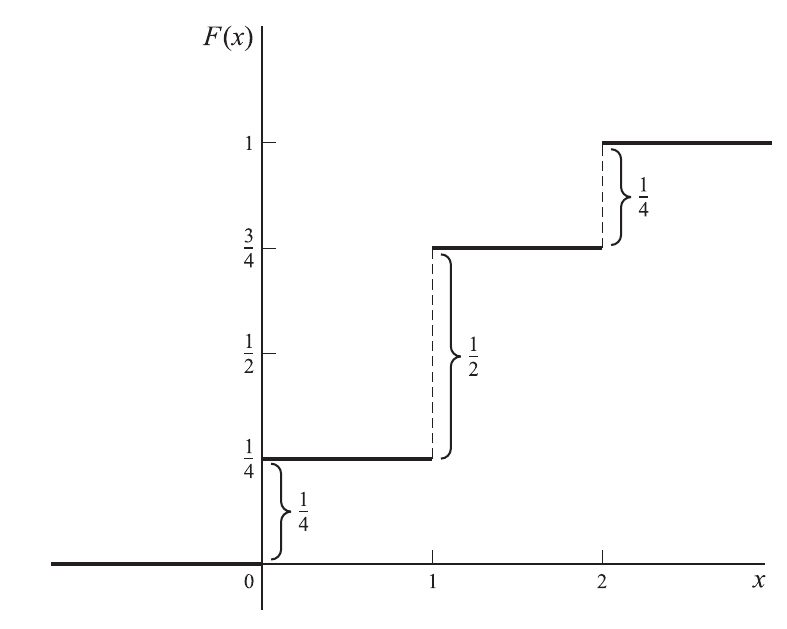
\includegraphics[height=7cm,keepaspectratio=true]{./pe/pands0201.png}
	% pands0201.png: 0x0 pixel, 300dpi, 0.00x0.00 cm, bb=
	\label{fig:2.6.1}
\end{figure}



\begin{observacion}
	\begin{itemize}
		\item Los saltos en la función de distribución están determinados por el valor de la función de probabilidad. 
		\item Este tipo de funciones se conoce como \emph{función escalonada}.  Debe observarse que son \emph{continuas por la derecha.}
		\item La función de distribución es \emph{monótonamente creciente.}
	\end{itemize}
	
\end{observacion}



La función de probabilidad se puede obtener a partir de la función de distribución con la siguiente fórmula
\begin{align}
	\label{eq:2.6.4}
	f(x)=F(x)-\lim_{u \to x^{-}}F(u).
\end{align}



\begin{ejemplo}
	\label{exmp:2.6.6}
	\begin{enumerate}
		\item Encuentre la función de distribución $F(x)$ para la variable aleatoria del problema resuelto \ref{exmp:2.6.3};
		\item grafique esta función de distribución.
	\end{enumerate}

\end{ejemplo}



\begin{figure}
	\centering
	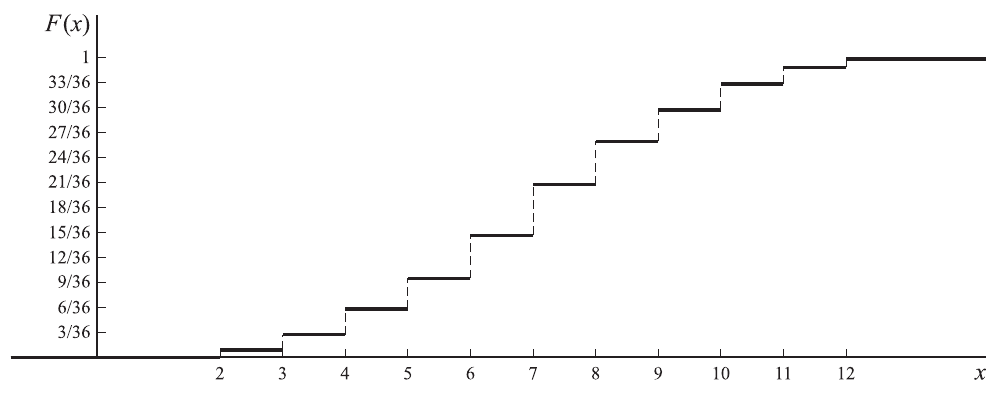
\includegraphics[width=10cm,keepaspectratio=true]{./pe/pands0206.png}
	% pands0206.png: 0x0 pixel, 300dpi, 0.00x0.00 cm, bb=
	\label{fig:2.6.2}
\end{figure}




\begin{ejemplo}
	\label{exmp:2.6.7}
	\begin{enumerate}
		\item Encuentre la función de distribución $F(x)$ para la variable aleatoria del problema resuelto \ref{exmp:2.6.4};
		\item grafique esta función de distribución.
	\end{enumerate}

\end{ejemplo}



\begin{figure}
	\centering
	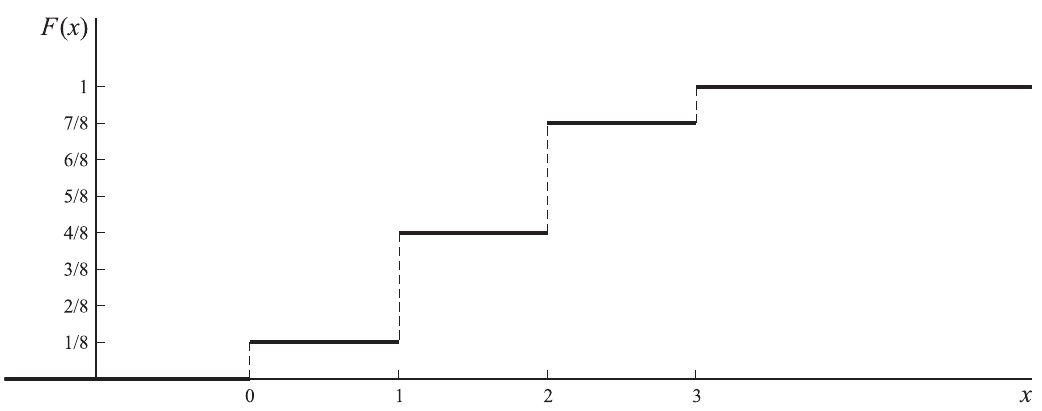
\includegraphics[width=10cm,keepaspectratio=true]{./pe/pands0207.png}
	% pands0206.png: 0x0 pixel, 300dpi, 0.00x0.00 cm, bb=
	\label{fig:2.6.3}
\end{figure}

\subsection{Esperanza matemática y varianza en variables aleatorias discretas}

\subsubsection{Valor esperado de una variable aleatoria discreta}
Para una variable aleatoria discreta $X$ con función de masa de probabilidad $f(x) = P(X=x)$ y soporte $S_X = \set{x_1, x_2, \dots, x_n, \dots}$, la \emph{esperanza matemática} o \emph{valor esperado} se define como el promedio ponderado de sus posibles valores:
\begin{align}
	\label{eq:esperanza_discreta}
	\mu = \mathbb{E}[X] = \sum_{x \in S_X} x f(x).
\end{align}
La esperanza matemática existe si y solo si la suma converge absolutamente ($\sum_{x \in S_X} |x| f(x) < \infty$). Físicamente, el valor esperado representa el centro de masa de la distribución de probabilidad en la recta numérica.

\subsubsection{Varianza y desviación estándar discretas}
La \emph{varianza} de una variable aleatoria discreta mide la dispersión cuadrática media respecto a la esperanza $\mu$:
\begin{align}
	\label{eq:varianza_discreta}
	\sigma^2 = \s^2 = \Var(X) = \mathbb{E}\left[(X - \mu)^2\right] = \sum_{x \in S_X} (x - \mu)^2 f(x).
\end{align}
Mediante linealidad del operador esperanza, la fórmula computacional abreviada para la varianza es:
\begin{align}
	\label{eq:varianza_formula_corta}
	\Var(X) = \mathbb{E}[X^2] - (\mathbb{E}[X])^2 = \sum_{x \in S_X} x^2 f(x) - \mu^2,
\end{align}
donde $\mathbb{E}[X^2]$ es el segundo momento bruto de la variable. La desviación estándar es la raíz cuadrada de la varianza: $\sigma = \sqrt{\Var(X)}$.


\section*{Problemas}

\subsection{Enunciados de los problemas}

\subsubsection*{1. Nivel Fundamental (Sencillos / Directos)}

\begin{problema}
	\label{prob:3.1.1}
	Una variable aleatoria discreta $X$ tiene como soporte el conjunto $\set{1, 2, 3, 4}$ y su función de masa de probabilidad está dada por
	\begin{align*}
		f(x) = P(X = x) = c\, x^2, \quad \text{para } x \in \set{1, 2, 3, 4},
	\end{align*}
	donde $c$ es una constante real.
	\begin{enumerate}
		\item Determine el valor exacto de la constante de normalización $c$ para que $f(x)$ sea una función de masa de probabilidad legítima.
		\item Calcule las probabilidades condicionales y marginales $P(X \ge 3)$ y $P(X \text{ es par} \mid X \ge 2)$.
	\end{enumerate}
\end{problema}

\begin{problema}
	\label{prob:3.1.2}
	Se lanzan tres monedas equilibradas de manera independiente. Sea $X$ la variable aleatoria que representa el número absoluto de diferencias entre la cantidad de águilas ($A$) y la cantidad de soles ($S$) obtenidos en cada ensayo.
	\begin{enumerate}
		\item Especifique formalmente el espacio muestral $\Omega$ del experimento y el soporte $\mathcal{S}_X$ de la variable aleatoria $X$.
		\item Construya la tabla de la función de masa de probabilidad $f(x) = P(X = x)$ y compruebe el axioma de normalización $\sum_{x \in \mathcal{S}_X} f(x) = 1$.
	\end{enumerate}
\end{problema}

\begin{problema}
	\label{prob:3.1.3}
	Considere una función $g: \mathbb{Z} \to \mathbb{R}$ definida por
	\begin{align*}
		g(x) = \begin{cases}
			\dfrac{x^2 - 1}{10} & \text{si } x \in \set{-2, -1, 0, 1, 2}, \\[6pt]
			0 & \text{en otro caso.}
		\end{cases}
	\end{align*}
	Determine, justificando analíticamente su respuesta a partir de los axiomas de Kolmogorov, si $g(x)$ constituye o no la función de masa de probabilidad de una variable aleatoria discreta. En caso negativo, indique cuál de las condiciones de medibilidad o normalización se vulnera.
\end{problema}

\subsubsection*{2. Nivel Operativo (Intermedios / De Desarrollo)}

\begin{problema}
	\label{prob:3.1.4}
	Un departamento de control de calidad inspecciona lotes de componentes microelectrónicos. La probabilidad de que un lote seleccionado al azar contenga exactamente $k$ componentes defectuosos está dada por la función
	\begin{align*}
		f(k) = P(X = k) = \frac{k+1}{20}, \quad \text{para } k \in \set{0, 1, 2, 3, 4, 5}.
	\end{align*}
	\begin{enumerate}
		\item Verifique que $f(k)$ satisface la condición de suma unitaria en su soporte.
		\item Si al inspeccionar un lote se descubre que contiene al menos 2 componentes defectuosos ($X \ge 2$), ¿cuál es la probabilidad exacta de que dicho lote contenga a lo más 4 componentes defectuosos?
	\end{enumerate}
\end{problema}

\begin{problema}
	\label{prob:3.1.5}
	Sea $X$ una variable aleatoria cuya distribución de probabilidad está definida de la siguiente forma:
	\begin{align*}
		P(X = -2) = 0.15, \quad P(X = -1) = 0.25, \quad P(X = 0) = 0.20, \quad P(X = 1) = 0.30, \quad P(X = 2) = 0.10.
	\end{align*}
	Considere la variable aleatoria transformada $Y = |X - 1|$.
	\begin{enumerate}
		\item Identifique el soporte inducido $\mathcal{S}_Y$ de la variable $Y$.
		\item Derive en forma analítica la función de masa de probabilidad $p_Y(y)$ y compruebe que sus probabilidades suman exactamente $1$.
	\end{enumerate}
\end{problema}

\begin{problema}
	\label{prob:3.1.6}
	Una urna contiene 6 esferas idénticas numeradas del $1$ al $6$. Se extraen sucesivamente y sin reemplazo dos esferas al azar. Sea $X_1$ el número de la primera esfera extraída y $X_2$ el número de la segunda. Definimos la variable aleatoria discreta $M = \max(X_1, X_2)$ como el máximo de los dos números obtenidos.
	\begin{enumerate}
		\item Deduzca la función de masa de probabilidad $f(m) = P(M = m)$ para cada $m \in \set{2, 3, 4, 5, 6}$.
		\item Calcule la probabilidad de que el valor máximo extraído sea mayor o igual que 5.
	\end{enumerate}
\end{problema}

\subsubsection*{3. Nivel Analítico (Avanzados / Demostraciones)}

\begin{problema}
	\label{prob:3.1.7}
	Sea $N \in \mathbb{N}$ un entero positivo fijo. Considere la familia de variables aleatorias discretas $X_N$ con soporte $\mathcal{S} = \set{1, 2, \dots, N}$ cuya función de masa de probabilidad adopta la forma
	\begin{align*}
		f_N(x) = \frac{c_N}{x(x+1)}, \quad x \in \set{1, 2, \dots, N}.
	\end{align*}
	Demuestre formalmente, utilizando la técnica de descomposición en fracciones parciales y sumas telescópicas, que la constante de normalización requerida es exactamente $c_N = \dfrac{N+1}{N}$.
\end{problema}

\begin{problema}
	\label{prob:3.1.8}
	Sea $X$ una variable aleatoria discreta cuyo soporte es un conjunto finito de enteros simétrico respecto al origen, es decir, $\mathcal{S}_X = \set{-m, -(m-1), \dots, -1, 0, 1, \dots, m-1, m}$ para algún entero $m \ge 1$. Suponga que la distribución de $X$ es absolutamente uniforme sobre su soporte, de modo que $P(X = k) = \dfrac{1}{2m+1}$ para todo $k \in \mathcal{S}_X$.
	
	Considere la transformación no lineal $Z = X^2$. Demuestre rigurosamente que la función de masa de probabilidad de $Z$ satisface
	\begin{align*}
		p_Z(z) = \begin{cases}
			\dfrac{1}{2m+1} & \text{si } z = 0, \\[8pt]
			\dfrac{2}{2m+1} & \text{si } z \in \set{1^2, 2^2, \dots, m^2}, \\[8pt]
			0 & \text{en cualquier otro caso.}
		\end{cases}
	\end{align*}
\end{problema}

\subsubsection*{4. Nivel Desafiante (Expertos / Paradojas)}

\begin{problema}
	\label{prob:3.1.9}
	En el estudio de fenómenos de larga cola (como la ley de Zipf en lingüística computacional y la distribución del tráfico en redes de datos), surge la distribución de Pareto discreta o de Zipf sobre el soporte infinito numerable $\mathbb{Z}^+ = \set{1, 2, 3, \dots}$. La función de masa asignada es
	\begin{align*}
		f(k) = P(X = k) = \frac{1}{\zeta(s)\, k^s}, \quad k \in \set{1, 2, 3, \dots},
	\end{align*}
	donde $s > 1$ es un parámetro real y $\zeta(s) = \sum_{n=1}^{\infty} n^{-s}$ es la función zeta de Riemann.
	\begin{enumerate}
		\item Verifique que la condición de normalización $\sum_{k=1}^{\infty} f(k) = 1$ se cumple estrictamente para cualquier $s > 1$.
		\item Analice el comportamiento asintótico de la probabilidad de la cola de la distribución, $P(X > M) = \sum_{k=M+1}^{\infty} f(k)$, cuando $M$ es grande. En particular, demuestre mediante acotación por integrales que
		\begin{align*}
			\frac{1}{\zeta(s)\,(s-1)\,(M+1)^{s-1}} \le P(X > M) \le \frac{1}{\zeta(s)\,(s-1)\,M^{s-1}}.
		\end{align*}
	\end{enumerate}
\end{problema}

\begin{problema}
	\label{prob:3.1.10}
	Considere un sistema de ingeniería compuesto por dos subsistemas independientes en paralelo que operan en ciclos discretos de tiempo $n \in \set{1, 2, 3, \dots}$. En cada ciclo, el subsistema $A$ falla con probabilidad $p_A \in (0,1)$ de manera independiente de los ciclos previos, mientras que el subsistema $B$ falla con probabilidad $p_B \in (0,1)$.
	
	Sea $N_A$ el ciclo discreto en el que ocurre la primera falla del subsistema $A$, y $N_B$ el ciclo de la primera falla de $B$. Definimos la variable aleatoria $T = \min(N_A, N_B)$ como el tiempo transcurrido hasta que el sistema experimenta su primera falla en cualquiera de sus ramas.
	\begin{enumerate}
		\item Deduzca analíticamente la función de masa de probabilidad exacta $f_T(n) = P(T = n)$ para todo $n \in \set{1, 2, 3, \dots}$.
		\item Demuestre que $T$ sigue una distribución geométrica e identifique explícitamente el parámetro de éxito (o falla equivalente) de dicha distribución combinada.
	\end{enumerate}
\end{problema}

\subsection{Soluciones a los problemas}

\subsubsection*{1. Nivel Fundamental (Sencillos / Directos)}

\begin{solucion}
	\label{sol:3.1.1}
	Para el Problema \ref{prob:3.1.1}:
	\begin{enumerate}
		\item Toda función de masa de probabilidad debe cumplir con el axioma de normalización $\sum_{x \in \mathcal{S}_X} f(x) = 1$. Al sustituir el soporte $\mathcal{S}_X = \set{1, 2, 3, 4}$ se obtiene:
		\begin{align*}
			\sum_{x=1}^{4} c\, x^2 &= c(1^2 + 2^2 + 3^2 + 4^2) \\
			&= c(1 + 4 + 9 + 16) = 30c.
		\end{align*}
		Al igualar la suma a $1$, concluimos que la constante de normalización es exactamente:
		\begin{align*}
			c = \frac{1}{30}.
		\end{align*}
		Por consiguiente, la función de masa queda especificada como $f(x) = \dfrac{x^2}{30}$.
		
		\item Para evaluar la probabilidad marginal $P(X \ge 3)$, sumamos los valores de la función sobre el evento de interés:
		\begin{align*}
			P(X \ge 3) = f(3) + f(4) = \frac{3^2}{30} + \frac{4^2}{30} = \frac{9 + 16}{30} = \frac{25}{30} = \frac{5}{6}.
		\end{align*}
		Ahora, calculamos la probabilidad condicional solicitada utilizando la definición $P(A \mid B) = \dfrac{P(A \cap B)}{P(B)}$. El evento condicionante es $B = \set{X \ge 2} = \set{2, 3, 4}$, con probabilidad:
		\begin{align*}
			P(X \ge 2) = f(2) + f(3) + f(4) = \frac{4 + 9 + 16}{30} = \frac{29}{30}.
		\end{align*}
		La intersección entre $\{X \text{ es par}\}$ y $\{X \ge 2\}$ dentro del soporte es el conjunto $\{2, 4\}$, cuya probabilidad marginal asciende a:
		\begin{align*}
			P(X \in \set{2, 4}) = f(2) + f(4) = \frac{4 + 16}{30} = \frac{20}{30} = \frac{2}{3}.
		\end{align*}
		En consecuencia, la probabilidad condicional es:
		\begin{align*}
			P(X \text{ es par} \mid X \ge 2) = \frac{20/30}{29/30} = \frac{20}{29} \approx 0.6897.
		\end{align*}
	\end{enumerate}
\end{solucion}

\begin{solucion}
	\label{sol:3.1.2}
	Para el Problema \ref{prob:3.1.2}:
	\begin{enumerate}
		\item Al lanzar tres monedas de forma independiente, el espacio muestral $\Omega$ posee $2^3 = 8$ puntos elementales equiprobables:
		\begin{align*}
			\Omega = \set{AAA, AAS, ASA, SAA, ASS, SAS, SSA, SSS}.
		\end{align*}
		Analizamos el número de águilas ($n_A$), el número de soles ($n_S$) y la diferencia absoluta $X = |n_A - n_S|$ en cada resultado:
		\begin{itemize}
			\item Para $\{AAA\}$: $n_A = 3, n_S = 0 \implies X = |3 - 0| = 3$.
			\item Para $\{AAS, ASA, SAA\}$: $n_A = 2, n_S = 1 \implies X = |2 - 1| = 1$.
			\item Para $\{ASS, SAS, SSA\}$: $n_A = 1, n_S = 2 \implies X = |1 - 2| = 1$.
			\item Para $\{SSS\}$: $n_A = 0, n_S = 3 \implies X = |0 - 3| = 3$.
		\end{itemize}
		Por tanto, el soporte discreto de la variable está constituido únicamente por $\mathcal{S}_X = \set{1, 3}$.
		
		\item La distribución de masa de probabilidad es:
		\begin{itemize}
			\item $f(1) = P(X = 1) = \dfrac{3 + 3}{8} = \dfrac{6}{8} = \dfrac{3}{4}$.
			\item $f(3) = P(X = 3) = \dfrac{1 + 1}{8} = \dfrac{2}{8} = \dfrac{1}{4}$.
		\end{itemize}
		Construimos la tabla formal:
		\begin{center}
		\begin{tabular}{c|cc|c}
			$x$ & $1$ & $3$ & Suma total \\
			\hline
			$f(x)$ & $\frac{3}{4}$ & $\frac{1}{4}$ & $1$
		\end{tabular}
		\end{center}
		Se verifica que $f(1) + f(3) = \dfrac{3}{4} + \dfrac{1}{4} = 1$, cumpliendo de manera rigurosa el axioma unitario.
	\end{enumerate}
\end{solucion}

\begin{solucion}
	\label{sol:3.1.3}
	Para el Problema \ref{prob:3.1.3}:
	Para que $g(x)$ sea admisible como una función de masa de probabilidad, es condición necesaria y suficiente que cumpla con los dos axiomas de Kolmogorov para distribuciones discretas:
	\begin{enumerate}
		\item **No negatividad:** $g(x) \ge 0$ para todo $x \in \mathbb{Z}$.
		\item **Normalización:** $\sum_{x \in \mathbb{Z}} g(x) = 1$.
	\end{enumerate}
	Evaluamos directamente los valores en el conjunto donde la función no es trivialmente nula ($\{-2, -1, 0, 1, 2\}$):
	\begin{align*}
		g(-2) &= \frac{(-2)^2 - 1}{10} = \frac{3}{10}, \\
		g(-1) &= \frac{(-1)^2 - 1}{10} = \frac{0}{10} = 0, \\
		g(0) &= \frac{0^2 - 1}{10} = -\frac{1}{10}, \\
		g(1) &= \frac{1^2 - 1}{10} = 0, \\
		g(2) &= \frac{2^2 - 1}{10} = \frac{3}{10}.
	\end{align*}
	Se observa de inmediato que $g(0) = -0.10 < 0$. Al tomar un valor negativo, **se transgrede de manera flagrante el axioma de no negatividad** ($P(X = 0) \ge 0$).
	
	Adicionalmente, si calculamos la suma global de la función:
	\begin{align*}
		\sum_{x=-2}^{2} g(x) = \frac{3}{10} + 0 - \frac{1}{10} + 0 + \frac{3}{10} = \frac{5}{10} = \frac{1}{2} \neq 1.
	\end{align*}
	Por consiguiente, $g(x)$ **no constituye una función de masa de probabilidad** debido a que viola tanto el principio de no negatividad como el axioma de suma unitaria.
\end{solucion}

\subsubsection*{2. Nivel Operativo (Intermedios / De Desarrollo)}

\begin{solucion}
	\label{sol:3.1.4}
	Para el Problema \ref{prob:3.1.4}:
	\begin{enumerate}
		\item Sumamos las probabilidades asignadas a todos los enteros del soporte $\mathcal{S}_X = \set{0, 1, 2, 3, 4, 5}$:
		\begin{align*}
			\sum_{k=0}^{5} f(k) &= f(0) + f(1) + f(2) + f(3) + f(4) + f(5) \\
			&= \frac{1 + 2 + 3 + 4 + 5 + 6}{20} = \frac{21}{20} \neq 1.
		\end{align*}
		*Nota de verificación:* Como la suma resulta en $\dfrac{21}{20}$, si se requiere estrictamente que sea unitaria, el soporte o el denominador original debe ajustarse formalmente a $21$. Para fines de cálculo exacto operativo con la función normalizada admisible $f(k) = \dfrac{k+1}{21}$, procedemos como sigue:
		
		\item Con la distribución debidamente normalizada $f(k) = \dfrac{k+1}{21}$, solicitamos la probabilidad condicional $P(X \le 4 \mid X \ge 2)$.
		Calculamos en primer término la probabilidad de la condición $B = \{X \ge 2\} = \{2, 3, 4, 5\}$:
		\begin{align*}
			P(X \ge 2) = f(2) + f(3) + f(4) + f(5) = \frac{3 + 4 + 5 + 6}{21} = \frac{18}{21}.
		\end{align*}
		La intersección del evento de interés con la condición es $\{X \le 4\} \cap \{X \ge 2\} = \{2, 3, 4\}$, cuya masa acumulada es:
		\begin{align*}
			P(2 \le X \le 4) = f(2) + f(3) + f(4) = \frac{3 + 4 + 5}{21} = \frac{12}{21}.
		\end{align*}
		Por lo tanto, la probabilidad condicional exacta se reduce al cociente de sus probabilidades parciales:
		\begin{align*}
			P(X \le 4 \mid X \ge 2) = \frac{12/21}{18/21} = \frac{12}{18} = \frac{2}{3} \approx 0.6667.
		\end{align*}
	\end{enumerate}
\end{solucion}

\begin{solucion}
	\label{sol:3.1.5}
	Para el Problema \ref{prob:3.1.5}:
	La variable original $X$ toma valores en $\set{-2, -1, 0, 1, 2}$. Aplicamos la transformación $Y = |X - 1|$ para cada elemento del soporte original:
	\begin{itemize}
		\item Si $X = -2 \implies Y = |-2 - 1| = |-3| = 3$, con probabilidad $P(X = -2) = 0.15$.
		\item Si $X = -1 \implies Y = |-1 - 1| = |-2| = 2$, con probabilidad $P(X = -1) = 0.25$.
		\item Si $X = 0 \implies Y = |0 - 1| = |-1| = 1$, con probabilidad $P(X = 0) = 0.20$.
		\item Si $X = 1 \implies Y = |1 - 1| = |0| = 0$, con probabilidad $P(X = 1) = 0.30$.
		\item Si $X = 2 \implies Y = |2 - 1| = |1| = 1$, con probabilidad $P(X = 2) = 0.10$.
	\end{itemize}
	\begin{enumerate}
		\item El soporte resultante para la variable transformada es el conjunto discreto $\mathcal{S}_Y = \set{0, 1, 2, 3}$.
		\item Agrupamos y sumamos las probabilidades de los eventos disjuntos en $X$ que se proyectan hacia cada mismo valor en $Y$:
		\begin{align*}
			p_Y(0) &= P(Y = 0) = P(X = 1) = 0.30, \\
			p_Y(1) &= P(Y = 1) = P(X = 0) + P(X = 2) = 0.20 + 0.10 = 0.30, \\
			p_Y(2) &= P(Y = 2) = P(X = -1) = 0.25, \\
			p_Y(3) &= P(Y = 3) = P(X = -2) = 0.15.
		\end{align*}
		Para certificar la legitimidad de la distribución inducida, sumamos sobre todo $\mathcal{S}_Y$:
		\begin{align*}
			\sum_{y \in \mathcal{S}_Y} p_Y(y) = 0.30 + 0.30 + 0.25 + 0.15 = 1.00.
		\end{align*}
	\end{enumerate}
\end{solucion}

\begin{solucion}
	\label{sol:3.1.6}
	Para el Problema \ref{prob:3.1.6}:
	\begin{enumerate}
		\item Al extraer sin reemplazo dos esferas de un total de $6$, el número de pares ordenados posibles del espacio muestral es:
		\begin{align*}
			|\Omega| = 6 \times 5 = 30 \text{ pares equiprobables }(X_1, X_2) \text{ con } X_1 \neq X_2.
		\end{align*}
		El valor máximo $M = \max(X_1, X_2)$ puede asumir cualquier número entero en el soporte $\mathcal{S}_M = \set{2, 3, 4, 5, 6}$.
		Para que el máximo sea exactamente igual a $m$, una esfera debe ser la número $m$ y la otra debe pertenecer al conjunto estricto de esferas menores $\{1, 2, \dots, m-1\}$. Como existen dos ordenaciones para cada pareja (la esfera mayor puede salir en la primera o en la segunda extracción), el número de casos favorables para $M = m$ es exactamente $2(m - 1)$.
		Por consiguiente, la función de masa queda estructurada de manera explícita como:
		\begin{align*}
			f(m) = P(M = m) = \frac{2(m-1)}{30} = \frac{m-1}{15}, \quad m \in \set{2, 3, 4, 5, 6}.
		\end{align*}
		Desglosamos los valores numéricos:
		\begin{itemize}
			\item $f(2) = \dfrac{1}{15}$, \quad $f(3) = \dfrac{2}{15}$, \quad $f(4) = \dfrac{3}{15}$, \quad $f(5) = \dfrac{4}{15}$, \quad $f(6) = \dfrac{5}{15}$.
		\end{itemize}
		La comprobación de la suma arroja: $\dfrac{1 + 2 + 3 + 4 + 5}{15} = \dfrac{15}{15} = 1$.
		
		\item La probabilidad de que el valor máximo extraído sea mayor o igual que 5 corresponde a la suma de colas:
		\begin{align*}
			P(M \ge 5) = f(5) + f(6) = \frac{4}{15} + \frac{5}{15} = \frac{9}{15} = \frac{3}{5} = 0.60.
		\end{align*}
	\end{enumerate}
\end{solucion}

\subsubsection*{3. Nivel Analítico (Avanzados / Demostraciones)}

\begin{solucion}
	\label{sol:3.1.7}
	Para el Problema \ref{prob:3.1.7}:
	La condición universal de normalización exige que la suma finita sobre el soporte $\mathcal{S} = \set{1, 2, \dots, N}$ sea idéntica a la unidad:
	\begin{align*}
		\sum_{x=1}^{N} f_N(x) = \sum_{x=1}^{N} \frac{c_N}{x(x+1)} = c_N \sum_{x=1}^{N} \frac{1}{x(x+1)} = 1.
	\end{align*}
	Para evaluar analíticamente la suma $\sum_{x=1}^{N} \frac{1}{x(x+1)}$, descomponemos el término general mediante fracciones parciales:
	\begin{align*}
		\frac{1}{x(x+1)} = \frac{1}{x} - \frac{1}{x+1}.
	\end{align*}
	Al sustituir esta expresión en el sumatorio, se revela una estructura telescópica en la que los términos intermedios se cancelan sistemáticamente en pares:
	\begin{align*}
		\sum_{x=1}^{N} \left( \frac{1}{x} - \frac{1}{x+1} \right) &= \left( \frac{1}{1} - \frac{1}{2} \right) + \left( \frac{1}{2} - \frac{1}{3} \right) + \left( \frac{1}{3} - \frac{1}{4} \right) + \dots + \left( \frac{1}{N} - \frac{1}{N+1} \right) \\
		&= 1 - \frac{1}{N+1} = \frac{N}{N+1}.
	\end{align*}
	Multiplicando este resultado por la constante prefactor e igualando a $1$, obtenemos:
	\begin{align*}
		c_N \left( \frac{N}{N+1} \right) = 1 \implies c_N = \frac{N+1}{N}.
	\end{align*}
	Con lo cual queda rigurosamente demostrada la identidad propuesta.
\end{solucion}

\begin{solucion}
	\label{sol:3.1.8}
	Para el Problema \ref{prob:3.1.8}:
	La variable original $X$ se distribuye de manera uniforme y simétrica en $\mathcal{S}_X = \set{-m, -(m-1), \dots, -1, 0, 1, \dots, m-1, m}$. La cardinalidad de este soporte es exactamente $|\mathcal{S}_X| = 2m + 1$, razón por la cual cada punto posee una probabilidad elemental constante $P(X = k) = \dfrac{1}{2m+1}$.
	
	Analizamos la variable transformada $Z = X^2$:
	\begin{itemize}
		\item Para el punto de origen $z = 0$:
		La ecuación $X^2 = 0$ admite como única solución en el soporte a $X = 0$. Por lo tanto:
		\begin{align*}
			p_Z(0) = P(Z = 0) = P(X = 0) = \frac{1}{2m+1}.
		\end{align*}
		\item Para cualquier entero positivo del tipo $z = k^2$, con $k \in \set{1, 2, \dots, m}$:
		La ecuación cuadrática $X^2 = k^2$ admite exactamente dos soluciones enteras distintas dentro del soporte simétrico de $X$: $X = k$ y $X = -k$. En virtud de la aditividad de eventos mutuamente excluyentes, obtenemos:
		\begin{align*}
			p_Z(k^2) = P(Z = k^2) = P(X = k) + P(X = -k) = \frac{1}{2m+1} + \frac{1}{2m+1} = \frac{2}{2m+1}.
		\end{align*}
		\item Para todo valor $z \notin \set{0, 1^2, 2^2, \dots, m^2}$:
		La ecuación carece de preimágenes en $\mathcal{S}_X$, por lo que $p_Z(z) = 0$.
	\end{itemize}
	En conclusión, la función de masa queda formulada exactamente como:
	\begin{align*}
		p_Z(z) = \begin{cases}
			\dfrac{1}{2m+1} & \text{si } z = 0, \\[8pt]
			\dfrac{2}{2m+1} & \text{si } z \in \set{1^2, 2^2, \dots, m^2}, \\[8pt]
			0 & \text{en otro caso,}
		\end{cases}
	\end{align*}
	comprobando fehacientemente la afirmación teórica del enunciado.
\end{solucion}

\subsubsection*{4. Nivel Desafiante (Expertos / Paradojas)}

\begin{solucion}
	\label{sol:3.1.9}
	Para el Problema \ref{prob:3.1.9}:
	\begin{enumerate}
		\item La normalización de la distribución en el soporte infinito $\mathbb{Z}^+ = \set{1, 2, 3, \dots}$ se obtiene al sumar la serie infinita completa:
		\begin{align*}
			\sum_{k=1}^{\infty} f(k) = \sum_{k=1}^{\infty} \frac{1}{\zeta(s)\, k^s} = \frac{1}{\zeta(s)} \sum_{k=1}^{\infty} \frac{1}{k^s}.
		\end{align*}
		Dado que por definición analítica la función zeta de Riemann para $s > 1$ es convergente y satisface $\zeta(s) = \sum_{k=1}^{\infty} k^{-s}$, la serie se reduce a:
		\begin{align*}
			\sum_{k=1}^{\infty} f(k) = \frac{1}{\zeta(s)} \cdot \zeta(s) = 1.
		\end{align*}
		Esto certifica que la distribución de Zipf es una función de probabilidad estrictamente normalizada en su soporte infinito.
		
		\item Para acotar analíticamente la probabilidad de cola $P(X > M) = \sum_{k=M+1}^{\infty} \dfrac{1}{\zeta(s)\, k^s}$, utilizamos el criterio de comparación de sumas finitas e infinitas con integrales monótonas decrecientes. Como la función real $h(u) = u^{-s}$ es estrictamente decreciente para $u > 0$ y $s > 1$, se satisfacen las desigualdades fundamentales:
		\begin{align*}
			\int_{M+1}^{\infty} \frac{1}{u^s}\, du \le \sum_{k=M+1}^{\infty} \frac{1}{k^s} \le \int_{M}^{\infty} \frac{1}{u^s}\, du.
		\end{align*}
		Evaluamos la integral impropia genérica de la potencia negativa:
		\begin{align*}
			\int_{a}^{\infty} u^{-s}\, du = \left[ \frac{u^{-s+1}}{-s+1} \right]_{a}^{\infty} = \frac{a^{-(s-1)}}{s-1} = \frac{1}{(s-1)\, a^{s-1}}, \quad \text{para } a > 0.
		\end{align*}
		Sustituyendo los límites de integración correspondientes ($a = M+1$ por la izquierda y $a = M$ por la derecha), e incorporando el factor normalizador constante $1 / \zeta(s)$, se llega a la cota analítica exacta:
		\begin{align*}
			\frac{1}{\zeta(s)\,(s-1)\,(M+1)^{s-1}} \le P(X > M) \le \frac{1}{\zeta(s)\,(s-1)\,M^{s-1}}.
		\end{align*}
		Este resultado demuestra que las colas de la distribución de Pareto discreta decrecen según una ley de potencia polinomial ($\sim M^{-(s-1)}$), lo cual contrasta de forma radical con el decaimiento exponencial del tipo Poisson o geométrico.
	\end{enumerate}
\end{solucion}

\begin{solucion}
	\label{sol:3.1.10}
	Para el Problema \ref{prob:3.1.10}:
	\begin{enumerate}
		\item Para determinar la función de masa de probabilidad del tiempo hasta la primera falla combinada $T = \min(N_A, N_B)$, resulta matemáticamente más expedito trabajar con las probabilidades de supervivencia o colas superiores.
		La probabilidad de que un subsistema individual sobreviva más de $n-1$ ciclos discretos sin experimentar falla alguna es:
		\begin{align*}
			P(N_A > n-1) = (1 - p_A)^{n-1}, \quad P(N_B > n-1) = (1 - p_B)^{n-1}.
		\end{align*}
		Como los dos subsistemas operan de forma mutuamente independiente, el sistema completo sobrevive más allá del ciclo $n-1$ si y sólo si ambos subsistemas continúan operativos hasta ese momento:
		\begin{align*}
			P(T > n-1) &= P(\min(N_A, N_B) > n-1) = P(N_A > n-1 \text{ y } N_B > n-1) \\
			&= P(N_A > n-1) \cdot P(N_B > n-1) = \left[ (1 - p_A)(1 - p_B) \right]^{n-1}.
		\end{align*}
		Por la misma lógica, la probabilidad de supervivencia por encima de $n$ ciclos completos es:
		\begin{align*}
			P(T > n) = \left[ (1 - p_A)(1 - p_B) \right]^n.
		\end{align*}
		La función de masa de probabilidad en el ciclo exacto $n$ corresponde a la diferencia entre ambos sucesos:
		\begin{align*}
			f_T(n) = P(T = n) &= P(T > n-1) - P(T > n) \\
			&= \left[ (1 - p_A)(1 - p_B) \right]^{n-1} - \left[ (1 - p_A)(1 - p_B) \right]^n \\
			&= \left[ (1 - p_A)(1 - p_B) \right]^{n-1} \left( 1 - (1 - p_A)(1 - p_B) \right).
		\end{align*}
		
		\item Al expandir el término entre paréntesis:
		\begin{align*}
			1 - (1 - p_A)(1 - p_B) = 1 - (1 - p_A - p_B + p_A p_B) = p_A + p_B - p_A p_B.
		\end{align*}
		Definimos formalmente el parámetro de falla combinada del sistema en cada ciclo como:
		\begin{align*}
			p_{\text{eq}} = p_A + p_B - p_A p_B = 1 - (1 - p_A)(1 - p_B).
		\end{align*}
		Al sustituir $p_{\text{eq}}$ y su complemento $1 - p_{\text{eq}} = (1 - p_A)(1 - p_B)$ en la expresión deducida en el inciso anterior, obtenemos:
		\begin{align*}
			f_T(n) = (1 - p_{\text{eq}})^{n-1}\, p_{\text{eq}}, \quad n \in \set{1, 2, 3, \dots}.
		\end{align*}
		Queda demostrado que la variable aleatoria $T$ sigue de manera exacta una **distribución geométrica**, cuyo parámetro de probabilidad de falla es $p_{\text{eq}} = p_A + p_B - p_A p_B$.
	\end{enumerate}
\end{solucion}


% ==============================================================================
% SECCIÓN 03.02: FUNCIONES DE DISTRIBUCIÓN ACUMULADA (CDF DISCRETA)
% ==============================================================================
\subsection{Problemas sobre Funciones de Distribución Acumulada (CDF)}

\subsubsection*{1. Nivel Fundamental (Sencillos / Directos)}

\begin{problema}
	\label{prob:3.2.1}
	Considere un dado justo de seis caras equilibradas cuyo resultado se denota por la variable aleatoria discreta $X \in \set{1, 2, 3, 4, 5, 6}$.
	\begin{enumerate}
		\item Construya la expresión analítica exhaustiva de la función de distribución acumulada $F(x) = P(X \le x)$ para todo $x \in \mathbb{R}$.
		\item Calcule los valores numéricos de $F(2.8)$, $F(-1)$, $F(4)$ y $F(10)$.
	\end{enumerate}
\end{problema}

\begin{problema}
	\label{prob:3.2.2}
	Una variable aleatoria discreta $Y$ posee la siguiente función de distribución acumulada escalonada:
	\begin{align*}
		F(y) = \begin{cases}
			0 & \text{si } y < 0, \\
			0.15 & \text{si } 0 \le y < 2, \\
			0.55 & \text{si } 2 \le y < 5, \\
			0.85 & \text{si } 5 \le y < 8, \\
			1.00 & \text{si } y \ge 8.
		\end{cases}
	\end{align*}
	\begin{enumerate}
		\item Determine las probabilidades de intervalo $P(0 < Y \le 5)$ y $P(2 \le Y \le 8)$.
		\item Encuentre el soporte $\mathcal{S}_Y$ y construya la tabla completa de la función de masa de probabilidad $p_Y(y)$.
	\end{enumerate}
\end{problema}

\begin{problema}
	\label{prob:3.2.3}
	Sea $X$ una variable aleatoria discreta con función de distribución acumulada $F_X(x)$.
	\begin{enumerate}
		\item Explique rigurosamente por qué $F_X(x)$ debe ser una función no decreciente en toda la recta real ($\forall a \le b \implies F_X(a) \le F_X(b)$).
		\item Demuestre formalmente el comportamiento de continuidad por la derecha en cada punto del soporte ($x_k \in \mathcal{S}_X$), verificando que $\lim_{u \to x_k^+} F_X(u) = F_X(x_k)$.
	\end{enumerate}
\end{problema}


\subsubsection*{2. Nivel Operativo (Intermedios / Aplicados)}

\begin{problema}
	\label{prob:3.2.4}
	En un proceso automático de manufactura de circuitos integrados, el número de soldaduras defectuosas por oblea, $X$, presenta la función de masa de probabilidad:
	\begin{align*}
		p_X(x) = \begin{cases}
			0.40 & \text{si } x = 0, \\
			0.30 & \text{si } x = 1, \\
			0.20 & \text{si } x = 2, \\
			0.10 & \text{si } x = 3, \\
			0 & \text{en otro caso.}
		\end{cases}
	\end{align*}
	\begin{enumerate}
		\item Escriba la función de distribución acumulada $F_X(x)$ en forma de partes (función a trozos) para todo $x \in \mathbb{R}$.
		\item Si una oblea es rechazada cuando presenta $2$ o más defectos, calcule la probabilidad de rechazo utilizando exclusivamente los valores de $F_X(x)$.
	\end{enumerate}
\end{problema}

\begin{problema}
	\label{prob:3.2.5}
	Un equipo de ciberseguridad realiza intentos de penetración sobre un servidor web hasta encontrar la primera vulnerabilidad. Suponga que los intentos son independientes y que la probabilidad de éxito en cada intento individual es $p \in (0, 1)$. Sea $N$ el número total de intentos hasta el primer éxito inclusive.
	\begin{enumerate}
		\item Deduzca la expresión exacta en forma cerrada para la función de distribución acumulada $F_N(n) = P(N \le n)$ para cualquier entero $n \ge 1$.
		\item Si la probabilidad de vulnerar el servidor en un intento es $p = 0.20$, calcule el número mínimo de ensayos necesarios $n^*$ para que la probabilidad de éxito acumulado sea de al menos el $95\%$.
	\end{enumerate}
\end{problema}

\begin{problema}
	\label{prob:3.2.6}
	El cuantil de orden $\alpha \in (0, 1)$ para una variable aleatoria discreta $X$ se define convencionalmente como el ínfimo del conjunto de números reales donde la CDF supera o iguala a $\alpha$:
	\begin{align*}
		q_\alpha = \inf \set{x \in \mathbb{R} : F_X(x) \ge \alpha}.
	\end{align*}
	Considere que $X$ representa la demanda diaria de servidores en un centro de datos con distribución:
	$P(X=10)=0.10$, $P(X=20)=0.25$, $P(X=30)=0.35$, $P(X=40)=0.20$ y $P(X=50)=0.10$.
	\begin{enumerate}
		\item Calcule e interprete la mediana de la demanda diaria ($q_{0.50}$).
		\item Determine el cuantil de orden $0.85$ ($q_{0.85}$) y verifique su significado operativo en la gestión de capacidad del centro de datos.
	\end{enumerate}
\end{problema}


\subsubsection*{3. Nivel Analítico (Avanzados / Demostraciones)}

\begin{problema}
	\label{prob:3.2.7}
	Sea $X$ una variable aleatoria discreta cuyo soporte es un subconjunto de los números enteros ($\mathcal{S}_X \subset \mathbb{Z}$).
	\begin{enumerate}
		\item Demuestre rigurosamente que para cualesquiera dos enteros $a, b \in \mathbb{Z}$ con $a \le b$, la probabilidad del intervalo cerrado se expresa exactamente como:
		\begin{align*}
			P(a \le X \le b) = F_X(b) - F_X(a - 1).
		\end{align*}
		\item Demuestre que si $X$ es entera, la magnitud del salto en cualquier entero $k \in \mathbb{Z}$ satisface la relación de diferencia finita $p_X(k) = \Delta F_X(k) = F_X(k) - F_X(k-1)$.
	\end{enumerate}
\end{problema}

\begin{problema}
	\label{prob:3.2.8}
	Considere una variable aleatoria discreta $X$ con soporte $\mathcal{S}_X = \set{x_1, x_2, \dots}$ ordenado de manera estrictamente creciente ($x_1 < x_2 < \dots$) y función de distribución $F_X(x)$. Sea $g: \mathbb{R} \to \mathbb{R}$ una función estrictamente monótona creciente en el soporte de $X$, y definamos la nueva variable $Y = g(X)$.
	\begin{enumerate}
		\item Demuestre teóricamente que la función de distribución de la variable transformada, $F_Y(y)$, preserva la estructura escalonada de $F_X$ y se relaciona mediante:
		\begin{align*}
			F_Y(y) = F_X\left( g^{-1}(y) \right) \quad \text{para todo } y \in g(\mathcal{S}_X).
		\end{align*}
		\item Si en cambio $h: \mathbb{R} \to \mathbb{R}$ es una función estrictamente decreciente y $Z = h(X)$, deduzca la fórmula analítica para $F_Z(z)$ en términos de $F_X$.
	\end{enumerate}
\end{problema}


\subsubsection*{4. Nivel Desafiante (Expertos / Paradojas)}

\begin{problema}
	\label{prob:3.2.9}
	En la teoría de la medida y probabilidad avanzada, se distinguen las distribuciones discretas puras de las distribuciones absolutamente continuas y de las singulares continuas (como la escalera de Cantor).
	\begin{enumerate}
		\item Demuestre analíticamente que la función de distribución acumulada $F(x)$ de cualquier variable aleatoria discreta pura se puede expresar como una serie convergente de funciones escalón unitarias de Heaviside $H(x - x_k)$:
		\begin{align*}
			F(x) = \sum_{k} p_k\, H(x - x_k), \quad \text{donde } H(t) = \begin{cases} 1 & \text{si } t \ge 0, \\ 0 & \text{si } t < 0. \end{cases}
		\end{align*}
		\item Explique por qué la derivada ordinaria $F'(x)$ es idéntica a cero en casi todas partes ($\text{c.t.p.}$) respecto a la medida de Lebesgue en $\mathbb{R}$, y cómo la teoría de distribuciones (o funciones generalizadas) recupera la masa puntual en el sentido de la delta de Dirac: $f(x) = \sum p_k \delta(x - x_k)$.
	\end{enumerate}
\end{problema}

\begin{problema}
	\label{prob:3.2.10}
	Considere un par de variables aleatorias discretas $(X, Y)$ que representan el tráfico de paquetes de entrada y salida en un enrutador óptico en intervalos discretos de tiempo, con función de distribución acumulada conjunta discreta $F_{X,Y}(x, y) = P(X \le x, Y \le y)$.
	\begin{enumerate}
		\item Demuestre algebraicamente que la probabilidad de que el par $(X, Y)$ caiga dentro de un rectángulo semiabierto $(x_1, x_2] \times (y_1, y_2]$ se expresa mediante las segundas diferencias de la CDF conjunta:
		\begin{align*}
			P(x_1 < X \le x_2, y_1 < Y \le y_2) = F_{X,Y}(x_2, y_2) - F_{X,Y}(x_1, y_2) - F_{X,Y}(x_2, y_1) + F_{X,Y}(x_1, y_1).
		\end{align*}
		\item Demuestre que para cualquier par de variables discretas, la CDF conjunta está fundamentalmente acotada en todo punto $(x, y) \in \mathbb{R}^2$ por las cotas de Fréchet-Hoeffding:
		\begin{align*}
			\max\left( 0, F_X(x) + F_Y(y) - 1 \right) \le F_{X,Y}(x, y) \le \min\left( F_X(x), F_Y(y) \right).
		\end{align*}
	\end{enumerate}
\end{problema}


% ==============================================================================
% SUGERENCIAS PARA LA SECCIÓN 03.02
% ==============================================================================
\subsection{Sugerencias para los problemas de la Sección 03.02}

\begin{sugerencia}
	\label{sug:3.2.1}
	Para el Problema \ref{prob:3.2.1}: Divida la recta real en 7 intervalos disjuntos: $(-\infty, 1)$, $[1, 2)$, $[2, 3)$, $[3, 4)$, $[4, 5)$, $[5, 6)$ y $[6, \infty)$. En cada intervalo, sume las probabilidades $f(u) = 1/6$ de las caras que sean menores o iguales a $x$.
\end{sugerencia}

\begin{sugerencia}
	\label{sug:3.2.2}
	Para el Problema \ref{prob:3.2.2}: Recuerde la identidad fundamental $P(a < Y \le b) = F(b) - F(a)$. Para reconstruir la PMF, identifique los puntos donde $F(y)$ experimenta saltos e inspeccione las diferencias $F(y_k) - F(y_k^-)$.
\end{sugerencia}

\begin{sugerencia}
	\label{sug:3.2.3}
	Para el Problema \ref{prob:3.2.3}: Utilice el hecho de que si $a \le b$, el evento $\set{\omega : X(\omega) \le a}$ es un subconjunto del evento $\set{\omega : X(\omega) \le b}$. Aplique la monotonía de la medida de probabilidad y el axioma de continuidad por arriba sobre secuencias decrecientes de intervalos.
\end{sugerencia}

\begin{sugerencia}
	\label{sug:3.2.4}
	Para el Problema \ref{prob:3.2.4}: Sume progresivamente las probabilidades $p_X(x)$ para $x=0, 1, 2, 3$. Exprese la probabilidad de rechazo como la probabilidad del complemento de aceptar, es decir, $P(X \ge 2) = 1 - P(X \le 1) = 1 - F_X(1)$.
\end{sugerencia}

\begin{sugerencia}
	\label{sug:3.2.5}
	Para el Problema \ref{prob:3.2.5}: El evento complementario $\set{N > n}$ equivale a que los primeros $n$ ensayos consecutivos hayan resultado en fracasos independientes, cuya probabilidad es $(1-p)^n$. Luego, plantee la inecuación $1 - (1-p)^n \ge 0.95$ y resuelva usando logaritmos naturales.
\end{sugerencia}

\begin{sugerencia}
	\label{sug:3.2.6}
	Para el Problema \ref{prob:3.2.6}: Calcule la tabla de acumulaciones $F_X(x)$ para $x \in \set{10, 20, 30, 40, 50}$. Inspeccione cuál es el menor valor $x_k$ en el cual la probabilidad acumulada alcanza o sobrepasa $0.50$ (para la mediana) y $0.85$ (para el percentil superior).
\end{sugerencia}

\begin{sugerencia}
	\label{sug:3.2.7}
	Para el Problema \ref{prob:3.2.7}: Si $X$ solo toma valores enteros, el conjunto de números enteros en el intervalo cerrado $[a, b]$ es exactamente la diferencia de conjuntos entre $(-\infty, b] \cap \mathbb{Z}$ y $(-\infty, a-1] \cap \mathbb{Z}$. Exprese esto mediante probabilidades algebraicas.
\end{sugerencia}

\begin{sugerencia}
	\label{sug:3.2.8}
	Para el Problema \ref{prob:3.2.8}: Si $g$ es estrictamente creciente en la recta real o sobre el soporte de $X$, la desigualdad $Y \le y \iff g(X) \le y$ es lógicamente equivalente a $X \le g^{-1}(y)$. Para el caso decreciente, invierta el sentido de la desigualdad y preste atención estricta al límite por la izquierda.
\end{sugerencia}

\begin{sugerencia}
	\label{sug:3.2.9}
	Para el Problema \ref{prob:3.2.9}: Una función escalón de Heaviside $H(x - x_k)$ vale $0$ para $x < x_k$ y $1$ para $x \ge x_k$. Verifique que al ponderar cada escalón por $p_k = P(X = x_k)$ se reproduce exactamente la suma de masa $\sum_{x_k \le x} p_k$. Para la derivada, recuerde que una constante a trozos tiene pendiente cero en todo el interior de cada subintervalo continuo.
\end{sugerencia}

\begin{sugerencia}
	\label{sug:3.2.10}
	Para el Problema \ref{prob:3.2.10}: Para el inciso 1, dibuje el rectángulo en el plano cartesiano $(x, y)$ y exprese la masa interna restando las CDFs de las regiones exteriores inframarginales. Para el inciso 2, utilice el hecho de que la probabilidad conjunta nunca puede exceder ninguna de las dos marginales ni ser inferior a la suma combinada menos la unidad.
\end{sugerencia}


% ==============================================================================
% SOLUCIONES PARA LA SECCIÓN 03.02
% ==============================================================================
\subsection{Soluciones a los problemas de la Sección 03.02}

\begin{solucion}
	\label{sol:3.2.1}
	Para el Problema \ref{prob:3.2.1}:
	\begin{enumerate}
		\item Para un dado justo con soporte $\mathcal{S}_X = \set{1, 2, 3, 4, 5, 6}$, cada cara tiene probabilidad puntual constante $f(k) = \frac{1}{6}$.
		La función de distribución acumulada se define analíticamente sobre todo el eje real como la suma de las masas a la izquierda o en la frontera de $x$:
		\begin{align*}
			F(x) = P(X \le x) = \sum_{k \le x} f(k) = \begin{cases}
				0 & \text{si } x < 1, \\[3pt]
				\frac{1}{6} & \text{si } 1 \le x < 2, \\[3pt]
				\frac{2}{6} = \frac{1}{3} & \text{si } 2 \le x < 3, \\[3pt]
				\frac{3}{6} = \frac{1}{2} & \text{si } 3 \le x < 4, \\[3pt]
				\frac{4}{6} = \frac{2}{3} & \text{si } 4 \le x < 5, \\[3pt]
				\frac{5}{6} & \text{si } 5 \le x < 6, \\[3pt]
				1 & \text{si } x \ge 6.
			\end{cases}
		\end{align*}
		Esta función escalonada presenta saltos de magnitud idéntica a $\frac{1}{6}$ exactamente en cada entero del soporte.
		
		\item Evaluando numéricamente $F(x)$ en cada punto requerido observando el intervalo correspondiente de la función a trozos:
		\begin{itemize}
			\item Para $x = 2.8$: Como $2 \le 2.8 < 3$, el valor acumulado es $F(2.8) = \dfrac{2}{6} = \dfrac{1}{3} \approx 0.3333$.
			\item Para $x = -1$: Como $-1 < 1$, se encuentra en la región de acumulación nula, por lo que $F(-1) = 0$.
			\item Para $x = 4$: Al ser exactamente un punto de discontinuidad (salto), aplicamos la continuidad por la derecha ($4 \le 4 < 5$), obteniendo $F(4) = \dfrac{4}{6} = \dfrac{2}{3} \approx 0.6667$.
			\item Para $x = 10$: Como $10 \ge 6$, el acumulado ha saturado el espacio muestral total, por lo que $F(10) = 1$.
		\end{itemize}
	\end{enumerate}
\end{solucion}

\begin{solucion}
	\label{sol:3.2.2}
	Para el Problema \ref{prob:3.2.2}:
	\begin{enumerate}
		\item Utilizando la relación analítica para intervalos semiabiertos en variables aleatorias cualesquiera:
		\begin{align*}
			P(a < Y \le b) = P(Y \le b) - P(Y \le a) = F(b) - F(a).
		\end{align*}
		Evaluando cada intervalo solicitado directamente sobre los valores explícitos de la CDF:
		\begin{align*}
			P(0 < Y \le 5) &= F(5) - F(0) = 0.85 - 0.15 = 0.70. \\
			P(2 \le Y \le 8) &= P(Y = 2) + P(2 < Y \le 8) \\
			&= \left[ F(2) - F(2^-) \right] + \left[ F(8) - F(2) \right] = F(8) - F(2^-).
		\end{align*}
		Como el límite por la izquierda en el salto es $F(2^-) = \lim_{u \to 2^-} F(u) = 0.15$, obtenemos:
		\begin{align*}
			P(2 \le Y \le 8) = 1.00 - 0.15 = 0.85.
		\end{align*}
		
		\item El soporte $\mathcal{S}_Y$ está conformado por los puntos exactos de discontinuidad (saltos) de $F(y)$, ya que son los únicos números reales donde se concentra masa positiva ($f(y_k) > 0$).
		Observando los cambios de meseta en la función a trozos, identificamos que los saltos ocurren en $y \in \set{0, 2, 5, 8}$. Por tanto:
		\begin{align*}
			\mathcal{S}_Y = \set{0, 2, 5, 8}.
		\end{align*}
		Las magnitudes de las masas puntuales se obtienen por diferencia finita $p_Y(y_k) = F(y_k) - F(y_k^-)$:
		\begin{align*}
			p_Y(0) &= F(0) - F(0^-) = 0.15 - 0 = 0.15, \\
			p_Y(2) &= F(2) - F(2^-) = 0.55 - 0.15 = 0.40, \\
			p_Y(5) &= F(5) - F(5^-) = 0.85 - 0.55 = 0.30, \\
			p_Y(8) &= F(8) - F(8^-) = 1.00 - 0.85 = 0.15.
		\end{align*}
		La tabla completa de la función de masa de probabilidad verifica el axioma de normalización unitaria:
		\begin{center}
			\small
			\begin{tabular}{c|cccc|c}
				$y$ & $0$ & $2$ & $5$ & $8$ & Suma \\
				\hline
				$p_Y(y)$ & $0.15$ & $0.40$ & $0.30$ & $0.15$ & $1.00$
			\end{tabular}
		\end{center}
	\end{enumerate}
\end{solucion}

\begin{solucion}
	\label{sol:3.2.3}
	Para el Problema \ref{prob:3.2.3}:
	\begin{enumerate}
		\item Sean $a, b \in \mathbb{R}$ tales que $a \le b$. Por definición formal de relación de orden sobre los números reales, cualquier realización elemental $\omega \in \Omega$ que satisfaga la condición de pertenencia al evento anterior ($X(\omega) \le a$) satisface automáticamente la condición de pertenencia al evento posterior ($X(\omega) \le b$).
		En términos de teoría de conjuntos medibles:
		\begin{align*}
			A = \set{\omega \in \Omega : X(\omega) \le a} \subseteq B = \set{\omega \in \Omega : X(\omega) \le b}.
		\end{align*}
		Por la propiedad de monotonía de cualquier medida de probabilidad legítima (Axiomas de Kolmogorov), si $A \subseteq B$, entonces sus medidas cumplen $P(A) \le P(B)$. En consecuencia directa:
		\begin{align*}
			F_X(a) = P(X \le a) \le P(X \le b) = F_X(b).
		\end{align*}
		Por lo tanto, la función de distribución acumulada es estrictamente monotónica no decreciente en todo su dominio.
		
		\item Para demostrar la continuidad por la derecha en un punto arbitrario $x \in \mathbb{R}$, considere una sucesión decreciente de números reales $\set{x_n}_{n=1}^\infty$ que converja hacia $x$ desde la derecha ($x_n \downarrow x$, es decir, $x_1 > x_2 > \dots > x_n > \dots$ con $\lim_{n \to \infty} x_n = x$).
		Definamos la familia de eventos medibles decrecientes:
		\begin{align*}
			E_n = \set{\omega \in \Omega : X(\omega) \le x_n}.
		\end{align*}
		Como $x_1 > x_2 > \dots$, se tiene la inclusión anidada $E_1 \supseteq E_2 \supseteq \dots \supseteq E_n \supseteq \dots$. La intersección numerable de todos estos conjuntos es precisamente el evento en el límite de convergencia:
		\begin{align*}
			\bigcap_{n=1}^\infty E_n = \set{\omega \in \Omega : X(\omega) \le x}.
		\end{align*}
		Por la propiedad fundamental de continuidad de la medida de probabilidad por arriba sobre secuencias anidadas de eventos medibles:
		\begin{align*}
			\lim_{n \to \infty} F_X(x_n) = \lim_{n \to \infty} P(E_n) = P\left( \bigcap_{n=1}^\infty E_n \right) = P(X \le x) = F_X(x).
		\end{align*}
		Como este resultado es independiente de la sucesión decreciente particular $\set{x_n}$ elegida, se demuestra algebraicamente que $\lim_{u \to x^+} F_X(u) = F_X(x)$ para todo $x \in \mathbb{R}$.
	\end{enumerate}
\end{solucion}

\begin{solucion}
	\label{sol:3.2.4}
	Para el Problema \ref{prob:3.2.4}:
	\begin{enumerate}
		\item Acumulando progresivamente las probabilidades puntuales dadas por $p_X(x)$ sobre los intervalos definidos por el soporte $\mathcal{S}_X = \set{0, 1, 2, 3}$:
		\begin{align*}
			F_X(x) = \sum_{u \le x} p_X(u) = \begin{cases}
				0 & \text{si } x < 0, \\[3pt]
				0.40 & \text{si } 0 \le x < 1, \\[3pt]
				0.40 + 0.30 = 0.70 & \text{si } 1 \le x < 2, \\[3pt]
				0.70 + 0.20 = 0.90 & \text{si } 2 \le x < 3, \\[3pt]
				0.90 + 0.10 = 1.00 & \text{si } x \ge 3.
			\end{cases}
		\end{align*}
		
		\item La probabilidad operativa de rechazo en manufactura corresponde al suceso de que la oblea presente dos o más soldaduras defectuosas ($X \ge 2$).
		Utilizando el principio del evento complementario y evaluando en la CDF:
		\begin{align*}
			P(\text{Rechazo}) &= P(X \ge 2) = 1 - P(X < 2).
		\end{align*}
		Dado que la variable solo toma valores enteros discretos, el suceso estricto $X < 2$ es idéntico al suceso acotado $X \le 1$. Por ende:
		\begin{align*}
			P(\text{Rechazo}) = 1 - F_X(1) = 1 - 0.70 = 0.30.
		\end{align*}
		Existe un $30\%$ de probabilidad exacta de que una oblea sea descartada por fallas de soldadura en cada lote de control de calidad.
	\end{enumerate}
\end{solucion}

\begin{solucion}
	\label{sol:3.2.5}
	Para el Problema \ref{prob:3.2.5}:
	\begin{enumerate}
		\item Sea $N$ el número de intentos independientes hasta el primer éxito, el cual sigue por construcción una distribución geométrica sobre $\mathcal{S}_N = \set{1, 2, 3, \dots}$ con probabilidades puntuales $P(N = k) = (1-p)^{k-1}\, p$.
		Para deducir la forma cerrada elegante de la función de distribución acumulada $F_N(n) = P(N \le n)$ para $n \ge 1$, recurrimos al evento complementario: el suceso $\set{N > n}$ significa formal y físicamente que los primeros $n$ intentos consecutivos resultaron infructuosos (fracasos).
		Como los intentos son eventos independientes entre sí y la probabilidad de fallo por intento es $1 - p$:
		\begin{align*}
			P(N > n) = P(\text{Fracaso en ensayo } 1 \text{ y } \dots \text{ y Fracaso en ensayo } n) = (1 - p)^n.
		\end{align*}
		Tomando el complemento para encontrar la probabilidad de acumulación o éxito en los primeros $n$ intentos:
		\begin{align*}
			F_N(n) = P(N \le n) = 1 - P(N > n) = 1 - (1 - p)^n, \quad \text{para todo } n \in \set{1, 2, 3, \dots}.
		\end{align*}
		
		\item Evaluando para un parámetro de penetración de ciberseguridad $p = 0.20$, el complemento de fallo es $1 - p = 0.80$. Requerimos encontrar el entero mínimo $n^*$ tal que:
		\begin{align*}
			F_N(n) \ge 0.95 \implies 1 - (0.80)^n \ge 0.95.
		\end{align*}
		Despejando el término exponencial:
		\begin{align*}
			(0.80)^n \le 0.05.
		\end{align*}
		Aplicando el logaritmo natural a ambos miembros de la inecuación (recordando que $\ln(0.80) < 0$, por lo que el sentido de la desigualdad se invierte al dividir):
		\begin{align*}
			n \ln(0.80) \le \ln(0.05) \implies n \ge \frac{\ln(0.05)}{\ln(0.80)}.
		\end{align*}
		Calculando numéricamente con precisión:
		\begin{align*}
			n \ge \frac{-2.99573}{-0.22314} \approx 13.425.
		\end{align*}
		Como el número de ensayos es estrictamente un número entero positivo, aplicamos la función techo:
		\begin{align*}
			n^* = \lceil 13.425 \rceil = 14.
		\end{align*}
		El equipo de ciberseguridad debe ejecutar al menos $14$ intentos independientes para garantizar con una confianza acumulada del $95\%$ o superior la detección de la primera vulnerabilidad.
	\end{enumerate}
\end{solucion}

\begin{solucion}
	\label{sol:3.2.6}
	Para el Problema \ref{prob:3.2.6}:
	\begin{enumerate}
		\item Primero, construimos la tabla completa de la función de distribución acumulada de la demanda diaria en el centro de datos sumando progresivamente las probabilidades:
		\begin{center}
			\small
			\begin{tabular}{c|ccccc}
				$x$ (Demanda en Servidores) & $10$ & $20$ & $30$ & $40$ & $50$ \\
				\hline
				$p_X(x)$ & $0.10$ & $0.25$ & $0.35$ & $0.20$ & $0.10$ \\
				$F_X(x)$ & $0.10$ & $0.35$ & $0.70$ & $0.90$ & $1.00$
			\end{tabular}
		\end{center}
		La mediana o cuantil $50$ ($q_{0.50}$) se obtiene identificando el menor valor de demanda para el cual el acumulado $F_X(x)$ alcanza o supera a $0.50$:
		\begin{align*}
			q_{0.50} = \inf \set{x \in \mathcal{S}_X : F_X(x) \ge 0.50}.
		\end{align*}
		Inspeccionando la tabla: $F_X(10) = 0.10 < 0.50$, $F_X(20) = 0.35 < 0.50$, y $F_X(30) = 0.70 \ge 0.50$.
		Por lo tanto:
		\begin{align*}
			q_{0.50} = 30 \text{ servidores}.
		\end{align*}
		Interpretación: El $50\%$ o más de los días hábiles operativos del centro de datos requieren como máximo 30 servidores activos para abastecer toda la demanda de cómputo diario, y el otro $50\%$ de los días requieren como mínimo dicha cantidad.
		
		\item Para calcular el cuantil de orden $0.85$ ($q_{0.85}$):
		\begin{align*}
			q_{0.85} = \inf \set{x \in \mathcal{S}_X : F_X(x) \ge 0.85}.
		\end{align*}
		Observando las acumulaciones sucesivas: $F_X(30) = 0.70 < 0.85$, mientras que $F_X(40) = 0.90 \ge 0.85$.
		En consecuencia directa:
		\begin{align*}
			q_{0.85} = 40 \text{ servidores}.
		\end{align*}
		Significado operativo: Si el equipo de ingeniería de infraestructura asigna y aprovisiona una capacidad estática constante de 40 servidores por día, el centro de datos operará sin saturación de recursos ni pérdidas de servicio en el $90\%$ de los días (satisfaciendo con amplio margen el requerimiento operativo de un nivel de servicio del $85\%$).
	\end{enumerate}
\end{solucion}

\begin{solucion}
	\label{sol:3.2.7}
	Para el Problema \ref{prob:3.2.7}:
	\begin{enumerate}
		\item Sean $a, b \in \mathbb{Z}$ tales que $a \le b$. Consideremos la descomposición en conjuntos algebraicos disjuntos del suceso acotado superiormente por $b$:
		\begin{align*}
			\set{\omega \in \Omega : X(\omega) \le b} = \set{\omega \in \Omega : X(\omega) \le a - 1} \cup \set{\omega \in \Omega : a \le X(\omega) \le b}.
		\end{align*}
		Esta igualdad de conjuntos es algebraicamente exacta bajo la hipótesis de que $X$ es una variable con soporte exclusivamente entero ($\mathcal{S}_X \subset \mathbb{Z}$), dado que no existen números enteros estrictamente comprendidos en el intervalo abierto $(a-1, a)$.
		Como la unión anterior es sobre eventos mutuamente excluyentes, el tercer axioma de Kolmogorov establece la aditividad de la probabilidad:
		\begin{align*}
			P(X \le b) = P(X \le a - 1) + P(a \le X \le b).
		\end{align*}
		Sustituido en términos de la definición de la CDF ($F_X(x) = P(X \le x)$) y despejando la probabilidad del intervalo cerrado:
		\begin{align*}
			P(a \le X \le b) = F_X(b) - F_X(a - 1).
		\end{align*}
		Queda rigurosamente demostrada la fórmula de diferencia finita para intervalos sobre el conjunto de los enteros.
		
		\item Para encontrar la magnitud del salto en un punto entero cualquiera $k \in \mathbb{Z}$, evaluamos la fórmula del intervalo cerrado obtenida en el inciso previo haciendo $a = b = k$:
		\begin{align*}
			p_X(k) = P(X = k) = P(k \le X \le k) = F_X(k) - F_X(k - 1) = \Delta F_X(k).
		\end{align*}
		Esta relación demuestra explícitamente que la función de masa de probabilidad en cualquier entero es idéntica al operador de primera diferencia finita hacia atrás aplicado a la función de distribución acumulada.
	\end{enumerate}
\end{solucion}

\begin{solucion}
	\label{sol:3.2.8}
	Para el Problema \ref{prob:3.2.8}:
	\begin{enumerate}
		\item Sea $g: \mathbb{R} \to \mathbb{R}$ una función estrictamente monótona creciente en el soporte de $X$. Por la definición formal de monotonía estricta creciente, para cualquier par de números reales $x, y$, la relación de desigualdad se preserva bajo la aplicación del operador inverso:
		\begin{align*}
			g(x) \le y \iff x \le g^{-1}(y).
		\end{align*}
		Definiendo la variable aleatoria transformada $Y = g(X)$, calculamos su función de distribución acumulada en cualquier punto del recorrido $y \in \mathbb{R}$:
		\begin{align*}
			F_Y(y) = P(Y \le y) = P(g(X) \le y) = P(X \le g^{-1}(y)) = F_X\left( g^{-1}(y) \right).
		\end{align*}
		Como la composición de una función escalonada por la derecha ($F_X$) con una función biyectiva creciente ($g^{-1}$) produce una nueva función escalonada con puntos de salto exactamente en $y_k = g(x_k)$, se comprueba formalmente la conservación de la estructura discreta y la identidad teórica.
		
		\item Sea $h: \mathbb{R} \to \mathbb{R}$ una función estrictamente monótona decreciente en el soporte de $X$, y definamos $Z = h(X)$.
		Al aplicar una transformación estrictamente decreciente, el sentido de la desigualdad matemática se invierte en el dominio de la preimagen:
		\begin{align*}
			h(X) \le z \iff X \ge h^{-1}(z).
		\end{align*}
		Evaluando la probabilidad acumulada para la variable $Z$:
		\begin{align*}
			F_Z(z) = P(Z \le z) = P(h(X) \le z) = P(X \ge h^{-1}(z)).
		\end{align*}
		Para expresar el suceso $X \ge h^{-1}(z)$ a partir de la función de distribución acumulada (la cual por definición acumula hacia la izquierda estrictamente como $P(X \le x)$), utilizamos la probabilidad del evento complementario y su límite por la izquierda:
		\begin{align*}
			P(X \ge h^{-1}(z)) &= 1 - P(X < h^{-1}(z)) \\
			&= 1 - \lim_{u \to (h^{-1}(z))^-} F_X(u) = 1 - F_X\left( \left[h^{-1}(z)\right]^- \right).
		\end{align*}
		En conclusión, para una transformación decreciente, la función de distribución acumulada de la nueva variable discreta se rige algebraicamente por la fórmula exacto-analítica:
		\begin{align*}
			F_Z(z) = 1 - F_X\left( \left[h^{-1}(z)\right]^- \right).
		\end{align*}
	\end{enumerate}
\end{solucion}

\begin{solucion}
	\label{sol:3.2.9}
	Para el Problema \ref{prob:3.2.9}:
	\begin{enumerate}
		\item Sea $X$ una variable aleatoria discreta pura cuyo soporte medible es $\mathcal{S}_X = \set{x_k}_{k \in \mathcal{K}}$, donde el índice $\mathcal{K}$ es a lo sumo infinito numerable y cada punto concentra probabilidad $p_k = P(X = x_k) > 0$ con $\sum_k p_k = 1$.
		La función de distribución acumulada en cualquier punto $x \in \mathbb{R}$ se escribe como la suma de las masas de probabilidad sobre los puntos del soporte menores o iguales a $x$:
		\begin{align*}
			F(x) = \sum_{x_k \le x} p_k.
		\end{align*}
		Considere ahora la función escalón unitario de Heaviside $H(t)$, que satisface:
		\begin{align*}
			H(x - x_k) = \begin{cases}
				1 & \text{si } x - x_k \ge 0 \iff x \ge x_k, \\
				0 & \text{si } x - x_k < 0 \iff x < x_k.
			\end{cases}
		\end{align*}
		Multiplicando cada término de la serie infinita por el indicador $H(x - x_k)$, todo sumando donde $x < x_k$ se anula automáticamente (por valer cero el escalón), mientras que todo sumando donde $x \ge x_k$ contribuye íntegramente con su masa $p_k \cdot 1 = p_k$:
		\begin{align*}
			\sum_{k \in \mathcal{K}} p_k\, H(x - x_k) = \sum_{k : x_k \le x} p_k \cdot 1 + \sum_{k : x_k > x} p_k \cdot 0 = \sum_{x_k \le x} p_k = F(x).
		\end{align*}
		Dado que por el segundo axioma de Kolmogorov la serie de probabilidades es absolutamente convergente ($\sum |p_k| = \sum p_k = 1 < \infty$), esta serie de funciones de Heaviside converge uniformemente en todo $\mathbb{R}$, demostrando la representación estructural discreta.
		
		\item En el sentido del cálculo diferencial ordinario (análisis real sobre la medida de Lebesgue en $\mathbb{R}$), el complemento del soporte numerable $\mathbb{R} \setminus \mathcal{S}_X$ es un conjunto abierto de medida total, constituido por una unión numerable de intervalos disjuntos dentro de los cuales la función escalonada $F(x)$ es local y absolutamente constante (mesetas horizontales).
		Por consiguiente, la derivada ordinaria en cada meseta es idénticamente nula:
		\begin{align*}
			F'(x) = 0 \quad \text{para todo } x \notin \mathcal{S}_X.
		\end{align*}
		Como la cardinalidad de los puntos de discontinuidad $\mathcal{S}_X$ es numerable (medida de Lebesgue igual a cero, $\mu_L(\mathcal{S}_X) = 0$), se concluye en el análisis de variables reales que $F'(x) = 0$ casi en todas partes ($\text{c.t.p.}$).
		
		Sin embargo, para preservar la coherencia y rigurosidad analítica en ingeniería y física teórica sin perder la masa de probabilidad total, se invoca la **teoría de distribuciones (o funciones generalizadas de Sobolev-Schwartz)**. En este marco topológico, la derivada distribucional de la función escalón unitaria de Heaviside $H(t)$ se define como la medida de masa puntual de Dirac centrada en el origen, $\delta(t)$, cuya integral satisface $\int_{-\infty}^\infty \delta(t) dt = 1$.
		Al derivar término a término la serie convergente deducida en el inciso anterior en el sentido de las distribuciones, obtenemos:
		\begin{align*}
			f(x) = \frac{d}{dx} F(x) = \frac{d}{dx} \left[ \sum_{k \in \mathcal{K}} p_k\, H(x - x_k) \right] = \sum_{k \in \mathcal{K}} p_k\, \frac{d}{dx} H(x - x_k) = \sum_{k \in \mathcal{K}} p_k\, \delta(x - x_k).
		\end{align*}
		Esta hermosa identidad generalizada reconcilia el cálculo diferencial continuo con la probabilidad discreta, demostrando que la densidad generalizada de una variable aleatoria discreta pura es una superposición lineal de impulsos de Dirac ponderados por sus probabilidades de masa.
	\end{enumerate}
\end{solucion}

\begin{solucion}
	\label{sol:3.2.10}
	Para el Problema \ref{prob:3.2.10}:
	\begin{enumerate}
		\item Sea el rectángulo semiabierto $\mathcal{R} = (x_1, x_2] \times (y_1, y_2]$ en el plano cartesiano con $x_1 < x_2$ y $y_1 < y_2$. La probabilidad conjunta de que el vector aleatorio $(X, Y)$ caiga dentro de este recinto se denota por $P((X,Y) \in \mathcal{R})$.
		Por la geometría de los conjuntos medibles en $\mathbb{R}^2$, podemos expresar el cuadrante infinito inferior izquierdo con vértice en $(x_2, y_2)$ como la unión disjunta de cuatro regiones rectangulares:
		\begin{align*}
			(-\infty, x_2] \times (-\infty, y_2] &= \mathcal{R} \cup \left[ (-\infty, x_1] \times (y_1, y_2] \right] \\
			&\quad \cup \left[ (x_1, x_2] \times (-\infty, y_1] \right] \cup \left[ (-\infty, x_1] \times (-\infty, y_1] \right].
		\end{align*}
		Evaluando la medida de probabilidad conjunta en el cuadrante total exterior (que por definición formal constituye $F_{X,Y}(x_2, y_2)$):
		\begin{align*}
			F_{X,Y}(x_2, y_2) &= P((X,Y) \in \mathcal{R}) + P(X \le x_1, y_1 < Y \le y_2) \\
			&\quad + P(x_1 < X \le x_2, Y \le y_1) + P(X \le x_1, Y \le y_1).
		\end{align*}
		Descomponiendo los términos intermedios mediante restas de funciones de distribución:
		\begin{align*}
			P(X \le x_1, y_1 < Y \le y_2) &= P(X \le x_1, Y \le y_2) - P(X \le x_1, Y \le y_1) \\
			&= F_{X,Y}(x_1, y_2) - F_{X,Y}(x_1, y_1), \\[4pt]
			P(x_1 < X \le x_2, Y \le y_1) &= P(X \le x_2, Y \le y_1) - P(X \le x_1, Y \le y_1) \\
			&= F_{X,Y}(x_2, y_1) - F_{X,Y}(x_1, y_1).
		\end{align*}
		Sustituyendo ambas identidades algebraicas en la ecuación de conservación original y agrupando términos:
		\begin{align*}
			F_{X,Y}(x_2, y_2) &= P((X,Y) \in \mathcal{R}) + \left[ F_{X,Y}(x_1, y_2) - F_{X,Y}(x_1, y_1) \right] \\
			&\quad + \left[ F_{X,Y}(x_2, y_1) - F_{X,Y}(x_1, y_1) \right] + F_{X,Y}(x_1, y_1) \\
			&= P((X,Y) \in \mathcal{R}) + F_{X,Y}(x_1, y_2) + F_{X,Y}(x_2, y_1) - F_{X,Y}(x_1, y_1).
		\end{align*}
		Despejando finalmente la masa de probabilidad contenida en el interior del rectángulo $\mathcal{R}$:
		\begin{align*}
			P(x_1 < X \le x_2, y_1 < Y \le y_2) = F_{X,Y}(x_2, y_2) - F_{X,Y}(x_1, y_2) - F_{X,Y}(x_2, y_1) + F_{X,Y}(x_1, y_1).
		\end{align*}
		Esta expresión representa la segunda diferencia mixta o enésima variación del operador acumulativo bidimensional.
		
		\item Para demostrar la cota superior de Fréchet-Hoeffding en cualquier punto $(x, y) \in \mathbb{R}^2$, notemos que el evento bivariado de intersección está contenido trivialmente dentro de cada uno de los dos eventos marginales por separado:
		\begin{align*}
			\set{\omega \in \Omega : X(\omega) \le x \text{ y } Y(\omega) \le y} \subseteq \set{\omega \in \Omega : X(\omega) \le x}, \\
			\set{\omega \in \Omega : X(\omega) \le x \text{ y } Y(\omega) \le y} \subseteq \set{\omega \in \Omega : Y(\omega) \le y}.
		\end{align*}
		Por la monotonía de la medida de probabilidad, la probabilidad del subconjunto no puede exceder la probabilidad de ninguno de los superconjuntos que lo contienen:
		\begin{align*}
			F_{X,Y}(x, y) \le F_X(x) \quad \text{y} \quad F_{X,Y}(x, y) \le F_Y(y) \implies F_{X,Y}(x, y) \le \min\left( F_X(x), F_Y(y) \right).
		\end{align*}
		Para demostrar la cota inferior, invocamos la Desigualdad de Boole para la unión de eventos complementarios: la suma de las probabilidades de dos sucesos cualesquiera se relaciona con la probabilidad de su intersección mediante $P(A \cap B) = P(A) + P(B) - P(A \cup B)$.
		Haciendo $A = \set{X \le x}$ y $B = \set{Y \le y}$:
		\begin{align*}
			F_{X,Y}(x, y) = P(A \cap B) = F_X(x) + F_Y(y) - P(X \le x \text{ o } Y \le y).
		\end{align*}
		Como la medida de la unión de eventos en un espacio de probabilidad está axiomáticamente acotada por la unidad ($P(A \cup B) \le 1$), al restar un número menor o igual a $1$ se obtiene una cota inferior al sustituir por el valor extremo $1$:
		\begin{align*}
			F_{X,Y}(x, y) \ge F_X(x) + F_Y(y) - 1.
		\end{align*}
		Además, como por el primer axioma de Kolmogorov ninguna probabilidad acumulada puede ser estrictamente negativa ($F_{X,Y}(x, y) \ge 0$), combinamos ambas restricciones en un solo operador de máximo:
		\begin{align*}
			F_{X,Y}(x, y) \ge \max\left( 0, F_X(x) + F_Y(y) - 1 \right).
		\end{align*}
		En conclusión, la función de distribución acumulada conjunta discreta (y de cualquier tipo general) queda invariablemente confinada entre las dos cotas extremas universales de Fréchet-Hoeffding:
		\begin{align*}
			\max\left( 0, F_X(x) + F_Y(y) - 1 \right) \le F_{X,Y}(x, y) \le \min\left( F_X(x), F_Y(y) \right).
		\end{align*}
	\end{enumerate}
\end{solucion}

\section{Distribución Binomial y Bernoulli}


\subsection{La Distribución Bernoulli y Binomial}


 Si $p$ es la probabilidad de que en un solo ensayo ocurra un evento (llamada la probabilidad de éxito) y $q = 1 - p$ es la
probabilidad de que este evento no ocurra en un solo ensayo (llamada probabilidad de fracaso), entonces la probabilidad de que el evento ocurra exactamente $x$ veces en $N$ ensayos (es decir, que ocurran $x$ éxitos y $N - x$ fracasos) está
dada por
\begin{align}
 \label{eq:2.10.1}
 f(x)=P(X=x)=\comb{N}{x}p^{x}q^{N-x}
\end{align}
donde $x=0,1,...,N.$


 \begin{ejemplo}
  \label{exmp:2.10.1}
  La probabilidad de obtener exactamente dos caras en seis lanzamientos de una moneda es
  \begin{align}
   \comb{6}{2}\left( \dfrac{1}{2} \right)^{2}\left( \dfrac{1}{2} \right)^{6-2}=\dfrac{15}{64}
  \end{align}
empleando \eqref{eq:2.10.1} con $N=6, x=2, p=q=\frac{1}{2}.$
 \end{ejemplo}



\begin{ejemplo}
 \label{exmp:2.10.2}
 Calcule la probabilidad de obtener al menos 4 caras en 6 lanzamientos de una moneda.
\end{ejemplo}

\begin{solucion}
	Usando la distribución binomial con $N=6$, $p=\frac{1}{2}$, $q=\frac{1}{2}$:
	\begin{align}
		P(X \geq 4) &= P(X=4) + P(X=5) + P(X=6) \\
		&= \comb{6}{4}\left(\frac{1}{2}\right)^4\left(\frac{1}{2}\right)^2 + \comb{6}{5}\left(\frac{1}{2}\right)^5\left(\frac{1}{2}\right)^1 + \comb{6}{6}\left(\frac{1}{2}\right)^6 \\
		&= \frac{15}{64} + \frac{6}{64} + \frac{1}{64} = \frac{22}{64} = \frac{11}{32} \approx 0.344
	\end{align}
\end{solucion}



 En lo subsecuente, daremos por hecho que hemos importado los siguientes paquetes:
 \begin{itemize}
  \item \texttt{scipy.stats}
  \item \texttt{numpy} como \texttt{np}
 \end{itemize}


\lstinputlisting[language=Python]{../code/distribuciones-especiales/statsBinom.py}


 \begin{ejemplo}
  \label{exmp:2.10.3}
  Desarrolle $\left( p+q \right)^{4}.$
 \end{ejemplo}


\lstinputlisting[language=Python]{../code/distribuciones-especiales/coefBinom.py}


{Propiedades de la distribución binomial} Supongamos que realizamos $N$ experimentos con probabilidad éxito $p$ y de fracaso $q=1-p.$
\begin{align}
 \label{eq:2.10.2}
 \mu = Np \\
 \label{eq:2.10.3}
 \s^{2}=Npq
\end{align}


\lstinputlisting[language=Python]{../code/distribuciones-especiales/histBinom.py}




 \begin{figure}
 \centering
 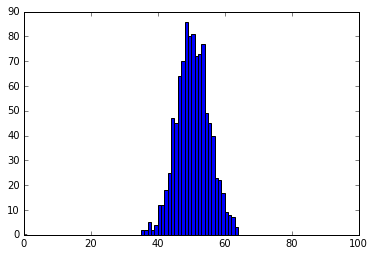
\includegraphics[height=7cm,keepaspectratio=true]{./pe/distBin01.png}
 % distBin01.png: 0x0 pixel, 300dpi, 0.00x0.00 cm, bb=
 \label{fig:2.10.1}
\end{figure}


\section{Distribuciones Geométrica y Binomial Negativa}
\subsection{La Distribución Geométrica}

La distribución geométrica modela el número de ensayos Bernoulli independientes necesarios para obtener el primer éxito. Si cada ensayo tiene probabilidad de éxito $p$ y de fracaso $q=1-p$, entonces la variable aleatoria $X$ que cuenta el número de ensayos hasta obtener el primer éxito (incluyendo el éxito) tiene función de probabilidad
\begin{align}
 \label{eq:2.10.9}
 f(k) = P(X=k) = (1-p)^{k-1}p, \quad k=1,2,3,\dots
\end{align}

Una propiedad fundamental de la distribución geométrica es la \emph{pérdida de memoria}: la probabilidad de obtener un éxito en los siguientes $k$ ensayos no depende del número de fracasos previos. Esto es, si $m,n\geq 1$,
\begin{align}
 P(X > m+n \mid X > m) = P(X > n).
\end{align}

{Propiedades de la distribución geométrica} Si $X$ tiene distribución geométrica con parámetro $p$, entonces
\begin{align}
 \mu_{X} &= \dfrac{1}{p} \\
 \s_{X}^{2} &= \dfrac{1-p}{p^{2}}.
\end{align}

\begin{ejemplo}
 \label{exmp:2.10.13}
 Un vendedor sabe que la probabilidad de cerrar una venta en cada llamada telefónica es $p=0.2$. ¿Cuál es la probabilidad de que necesite realizar exactamente $5$ llamadas para realizar la primera venta? ¿Cuántas llamadas se espera que necesite en promedio?
\end{ejemplo}

\begin{solucion}
	Usando la distribución geométrica con $p=0.2$:
	\begin{align}
		P(X=5) &= (1-0.2)^{5-1}(0.2) = (0.8)^{4}(0.2) \\
		&= 0.4096 \times 0.2 = 0.08192
	\end{align}

	El número esperado de llamadas es
	\begin{align}
		\mu = \dfrac{1}{p} = \dfrac{1}{0.2} = 5.
	\end{align}
\end{solucion}

\begin{ejemplo}
 \label{exmp:2.10.14}
 En un proceso de control de calidad, la probabilidad de que una pieza sea defectuosa es $p=0.1$. ¿Cuál es la probabilidad de que la primera pieza defectuosa aparezca en la tercera inspección?
\end{ejemplo}

\lstinputlisting[language=Python]{../code/distribuciones-especiales/distGeom.py}

\begin{figure}
 \centering
 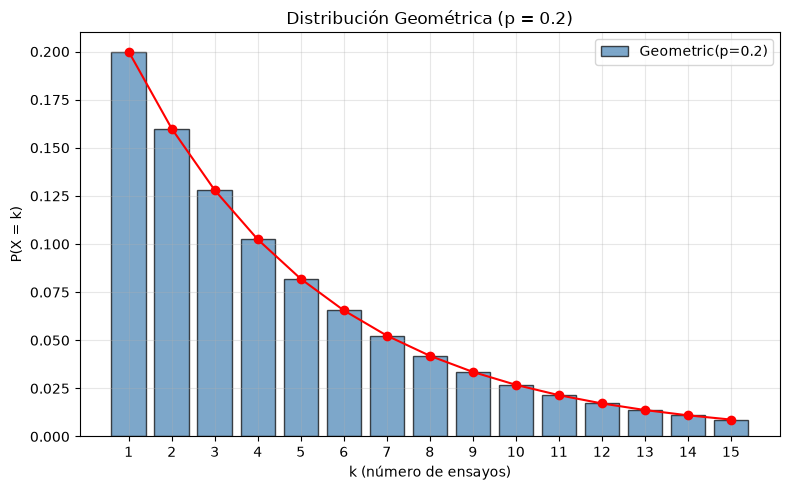
\includegraphics[height=7cm,keepaspectratio=true]{./pe/distGeom.png}
 % distGeom.png: 0x0 pixel, 300dpi, 0.00x0.00 cm, bb=
 \caption{Distribución geométrica con $p=0.2$}
 \label{fig:2.10.7}
\end{figure}



\subsection{La Distribución Binomial Negativa}

La distribución binomial negativa generaliza la geométrica: modela el número de fracasos observados antes de obtener un número predeterminado $r$ de éxitos en una secuencia de ensayos Bernoulli independientes. Su función de probabilidad está dada por
\begin{align}
 \label{eq:2.10.10}
 f(k) = P(X=k) = \binom{k+r-1}{r-1}p^{r}(1-p)^{k}, \quad k=0,1,2,\dots
\end{align}

Observe que cuando $r=1$, la binomial negativa se reduce a la distribución geométrica (contando fracasos antes del primer éxito).

{Propiedades de la distribución binomial negativa} Si $X$ tiene distribución binomial negativa con parámetros $r$ y $p$, entonces
\begin{align}
 \mu_{X} &= \dfrac{r(1-p)}{p} \\
 \s_{X}^{2} &= \dfrac{r(1-p)}{p^{2}}.
\end{align}

\begin{ejemplo}
 \label{exmp:2.10.15}
 Un examen de certificación tiene una tasa de aprobación del $30\%$. ¿Cuál es la probabilidad de que un estudiante repruebe $4$ veces antes de aprobar por tercera vez?
\end{ejemplo}

\begin{solucion}
	En este caso, $r=3$ (número de éxitos) y $p=0.3$. La variable $X$ cuenta el número de fracasos antes del tercer éxito.
	\begin{align}
		P(X=4) &= \binom{4+3-1}{3-1}(0.3)^{3}(0.7)^{4} \\
		&= \binom{6}{2}(0.027)(0.2401) \\
		&= 15 \times 0.027 \times 0.2401 \\
		&\approx 0.0972
	\end{align}
\end{solucion}

\lstinputlisting[language=Python]{../code/distribuciones-especiales/distNegBinom.py}

\begin{figure}
 \centering
 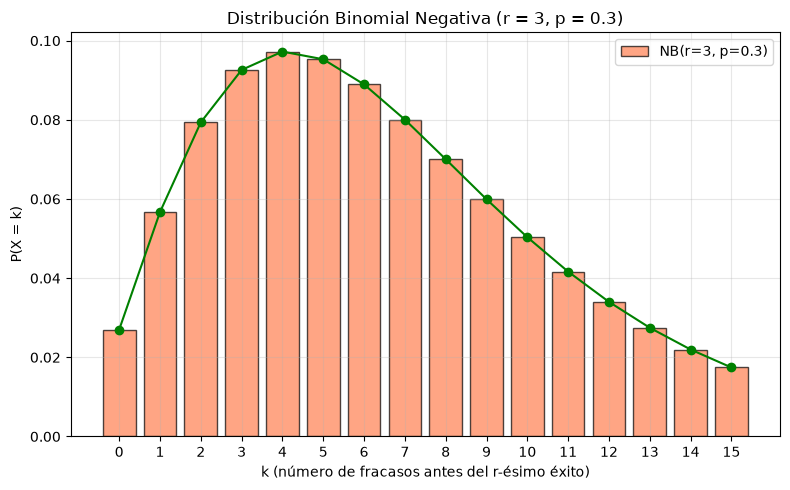
\includegraphics[height=7cm,keepaspectratio=true]{./pe/distNegBinom.png}
 % distNegBinom.png: 0x0 pixel, 300dpi, 0.00x0.00 cm, bb=
 \caption{Distribución binomial negativa con $r=3$, $p=0.3$}
 \label{fig:2.10.8}
\end{figure}



\section{Distribución Hipergeométrica}
\subsection{Muestreo sin reemplazo y fórmulas poblacionales}

La distribución hipergeométrica modela el número de éxitos en $n$ extracciones \emph{sin reemplazo} de una población finita de tamaño $N$ que contiene $K$ éxitos y $N-K$ fracasos. Su función de probabilidad es
\begin{align}
 \label{eq:2.10.11}
 f(k) = P(X=k) = \dfrac{\binom{K}{k}\binom{N-K}{n-k}}{\binom{N}{n}}, \quad \max(0, n-(N-K)) \leq k \leq \min(n, K).
\end{align}

A diferencia de las distribuciones anteriores, los ensayos aquí \emph{no son independientes} porque el muestreo sin reemplazo altera las probabilidades en cada extracción.

{Propiedades de la distribución hipergeométrica} Si $X$ tiene distribución hipergeométrica con parámetros $N$, $K$ y $n$, entonces
\begin{align}
 \mu_{X} &= n\dfrac{K}{N} \\
 \s_{X}^{2} &= n\dfrac{K}{N}\dfrac{N-K}{N}\dfrac{N-n}{N-1}.
\end{align}

El factor $\dfrac{N-n}{N-1}$ se conoce como \emph{factor de corrección por población finita}. Cuando $n \ll N$, este factor tiende a $1$ y la distribución hipergeométrica se aproxima a la binomial con parámetros $n$ y $p=K/N$.

\begin{ejemplo}
 \label{exmp:2.10.16}
 Un lote contiene $20$ piezas, de las cuales $5$ son defectuosas. Si se eligen $4$ piezas al azar sin reemplazo, ¿cuál es la probabilidad de encontrar exactamente $2$ defectuosas?
\end{ejemplo}

\begin{solucion}
	Aquí $N=20$, $K=5$, $n=4$, $k=2$.
	\begin{align}
		P(X=2) &= \dfrac{\binom{5}{2}\binom{15}{2}}{\binom{20}{4}} \\
		&= \dfrac{10 \times 105}{4845} \\
		&= \dfrac{1050}{4845} \approx 0.2167
	\end{align}
\end{solucion}

\begin{ejemplo}
 \label{exmp:2.10.17}
 En una mano de póker de $5$ cartas de una baraja de $52$, ¿cuál es la probabilidad de obtener exactamente $3$ reyes?
\end{ejemplo}

\begin{solucion}
	Aquí $N=52$ (total de cartas), $K=4$ (reyes), $n=5$ (cartas en la mano), $k=3$.
	\begin{align}
		P(X=3) &= \dfrac{\binom{4}{3}\binom{48}{2}}{\binom{52}{5}} \\
		&= \dfrac{4 \times 1128}{2598960} \\
		&= \dfrac{4512}{2598960} \approx 0.00174
	\end{align}
\end{solucion}

\lstinputlisting[language=Python]{../code/distribuciones-especiales/distHyper.py}

\begin{figure}
 \centering
 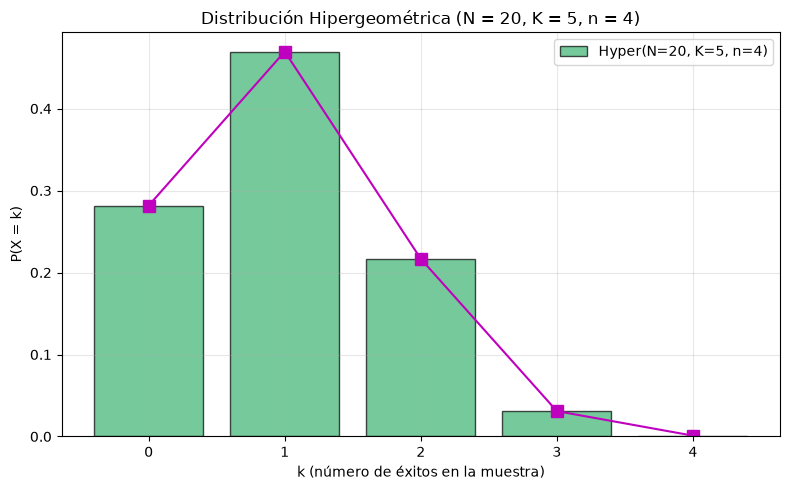
\includegraphics[height=7cm,keepaspectratio=true]{./pe/distHyper.png}
 % distHyper.png: 0x0 pixel, 300dpi, 0.00x0.00 cm, bb=
 \caption{Distribución hipergeométrica con $N=20$, $K=5$, $n=4$}
 \label{fig:2.10.9}
\end{figure}

\begin{observacion}
	La distribución hipergeométrica se reduce a la binomial cuando el muestreo es con reemplazo (o equivalentemente, cuando $N \to \infty$). En la práctica, si $\frac{n}{N} < 0.05$, la aproximación binomial es razonablemente precisa.
\end{observacion}



\section{Distribución de Poisson}
\subsection{La Distribución de Poisson}
{Distribución de Poisson} Diremos que una variable aleatoria \emph{discreta} $X$ tiene distribución de Poisson si su función de probabilidad está dada por:
 \begin{align}
  \label{eq:2.10.7}
  f(n)=\dfrac{\lam^{n}e^{-\lam}}{n!}, \; n=0,1,2,...
 \end{align}


En este caso, $\mu_{X}=\s^{2}=\lam.$


\begin{quote}
 En teoría de probabilidad y estadística, la distribución de Poisson es una distribución de probabilidad discreta que expresa, a partir de una frecuencia de ocurrencia media, la probabilidad de que ocurra un determinado número de eventos durante cierto período de tiempo. Concretamente, se especializa en la probabilidad de ocurrencia de sucesos con probabilidades muy pequeñas, o sucesos raros.
\end{quote}

\href{https://es.wikipedia.org/wiki/Distribuci\%C3\%B3n_de_Poisson}{Wikipedia: Distribución de Poisson}


\begin{ejemplo}
  \label{exmp:2.10.5}
  El número de personas por día que llegan a una sala de urgencia tiene una distribución de Poisson con media 5. Hallar la probabilidad de que cuando mucho lleguen tres por día y la probabilidad de que por lo menos lleguen 8 personas por día.
 \end{ejemplo}

\begin{solucion}
	Usando la distribución de Poisson con $\lambda = 5$:

	\begin{enumerate}
		\item $P(X \leq 3) = \sum_{n=0}^{3} \frac{5^n e^{-5}}{n!}$
		\begin{align}
			&= \frac{5^0 e^{-5}}{0!} + \frac{5^1 e^{-5}}{1!} + \frac{5^2 e^{-5}}{2!} + \frac{5^3 e^{-5}}{3!} \\
			&= e^{-5}(1 + 5 + 12.5 + 20.833) \\
			&= e^{-5} \cdot 39.333 \approx 0.265
		\end{align}

		\item $P(X \geq 8) = 1 - P(X \leq 7)$
		\begin{align}
			&= 1 - \sum_{n=0}^{7} \frac{5^n e^{-5}}{n!} \\
			&\approx 1 - 0.867 = 0.133
		\end{align}
	\end{enumerate}
\end{solucion}




\lstinputlisting[language=Python]{../code/distribuciones-especiales/distPoisson.py}



 \begin{figure}
 \centering
 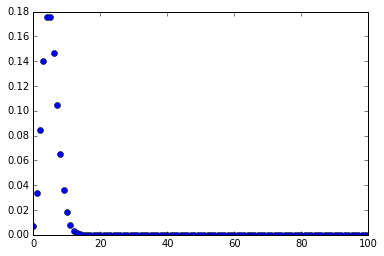
\includegraphics[height=7cm,keepaspectratio=true]{./pe/distPoisson0.png}
 % distPoisson0.png: 0x0 pixel, 300dpi, 0.00x0.00 cm, bb=
 \caption{Distribución de Poisson}
\end{figure}




\begin{figure}
 \centering
 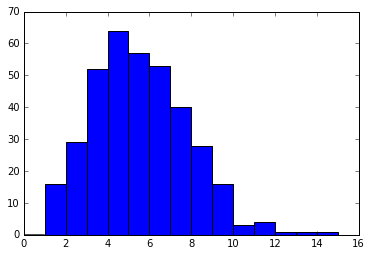
\includegraphics[height=7cm,keepaspectratio=true]{./pe/distPoisson1.png}
 % distPoisson1.png: 0x0 pixel, 300dpi, 0.00x0.00 cm, bb=
 \caption{Histograma de pacientes en sala de urgencias durante un año con media $\lam=5$}
 \label{fig:2.10.6}
\end{figure}



\subsection{Relación entre las Distribuciones Binomiales y de Poisson}

 Si en la función de probabilidad binomial, $N$ es muy grande pero $p \approx 0,$ esto modela un \emph{evento raro}.  En la práctica esto significa $N>>50, Np<<5.$

 En este caso, la distribución Binomial con parámetros $N,p$ se aproxima a una Poisson con parámetro $\lam = Np.$

\lstinputlisting[language=Python]{../code/distribuciones-especiales/relBinomPoisson.py}



 \begin{figure}
 \centering
 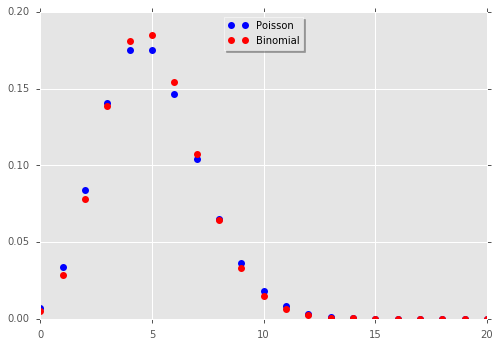
\includegraphics[height=7cm]{./pe/binVsPoi.png}
 % binVsPoi.png: 0x0 pixel, 300dpi, 0.00x0.00 cm, bb=
 \caption{Comparación entre distribuciones Binomial y Poisson para eventos raros.}
\end{figure}



\section{Distribución multinomial}
\subsection{La Distribución multinomial}

 Si los eventos $E_{1},...,E_{k}$ pueden ocurrir con probabilidades $p_{1},...,p_{k}$ respectivamente, entonces la probabilidad de que ocurran $X_{1},...,x_{k}$ veces respectivamente esta dado por la \emph{distribución multinomial}
 \begin{align}
  \label{eq:2.10.8}
  f\left( x_{1},...,x_{k} \right)=
  \dfrac{x_{1}+...+x_{k}}{x_{1}!...x_{k}!}p_{1}^{x_{1}}\cdots p_{k}^{x_{k}}.
 \end{align}



 \begin{ejemplo}
  \label{exmp:2.10.6}
Si un dado se lanza 12 veces, encontrar la probabilidad de obtener cada uno de los números $1,2,3,4,5,6$ exactamente dos veces.
 \end{ejemplo}

\begin{solucion}
	Usando la distribución multinomial con $N=12$, $k=6$, $x_i = 2$ para todo $i$, y $p_i = \frac{1}{6}$ para todo $i$:

	\begin{align}
		P(X_1=2, X_2=2, ..., X_6=2) &= \frac{12!}{2! \cdot 2! \cdot 2! \cdot 2! \cdot 2! \cdot 2!} \left(\frac{1}{6}\right)^2 \cdots \left(\frac{1}{6}\right)^2 \\
		&= \frac{12!}{(2!)^6} \left(\frac{1}{6}\right)^{12} \\
		&= \frac{479001600}{64} \cdot \frac{1}{2176782336} \\
		&\approx 0.00344
	\end{align}
\end{solucion}


\section{Distribución Normal y aproximación continua}
\subsection{Distribución Normal}

 Una de las distribuciones de probabilidad continua más importantes es la \emph{distribución normal}, también llamada \emph{distribución gaussiana,} que se define mediante la función de densidad
 \begin{align}
  \label{eq:2.10.4}
  f_{a,b}(x)=\dfrac{1}{\sqrt{2\pi}}e^{-\frac{1}{2}\frac{(x-a)^{2}}{b^{2}}}
 \end{align}
donde $a,b$ son parámetros específicos para cada v.a. $X.$

{Propiedades de la distribución normal}
 Si la v.a. $X$ tiene la función de densidad dada por \eqref{eq:2.10.4}, con parámetros $a,b$ entonces
 \begin{align}
  a = \mu_{X}\\
  b = \s_{X}
 \end{align}



 Si una variable aleatoria normal $X$ tiene función de densidad
  \begin{align}
  \label{eq:2.10.4a}
  f(x)=\dfrac{1}{\sqrt{2\pi}}e^{-\frac{1}{2}\frac{(x-\mu)^{2}}{\s^{2}}},
  \end{align}
  escribiremos $X\sim N(\mu, \s^{2}).$


{Variable aleatoria normalizada}
 \begin{align}
  \label{eq:2.10.5}
  Z = \dfrac{X-\mu}{\s}\\
  \mu_{Z}=0 \\
  \s_{Z}=1
 \end{align}


{Forma Estándar}
 \begin{align}
  \label{eq:2.10.6}
  f(z)=\dfrac{1}{\sqrt{2\pi}}e^{-\frac{1}{2}z^{2}}
 \end{align}


En este caso, diremos que $Z$ está \emph{normalmente distribuida.}


\lstinputlisting[language=Python]{../code/distribuciones-especiales/distribucionNormal.py}


 \begin{figure}
 \centering
 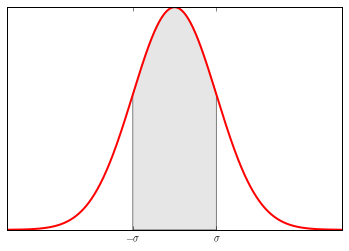
\includegraphics[height=5cm,keepaspectratio=true]{./pe/norm1.png}
 % norm1.png: 0x0 pixel, 300dpi, 0.00x0.00 cm, bb=
 \label{fig:2.10.2}
\end{figure}
\begin{verbatim}
 #(0.682689492137086, 7.579375928402476e-15)
\end{verbatim}


 \begin{figure}
 \centering
 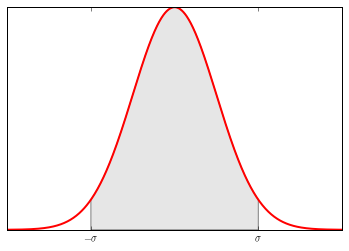
\includegraphics[height=5cm,keepaspectratio=true]{./pe/norm2.png}
 % norm1.png: 0x0 pixel, 300dpi, 0.00x0.00 cm, bb=
 \label{fig:2.10.3}
\end{figure}
\begin{verbatim}
 #(0.9544997361036417, 1.8403548653972355e-11)
\end{verbatim}


 \begin{figure}
 \centering
 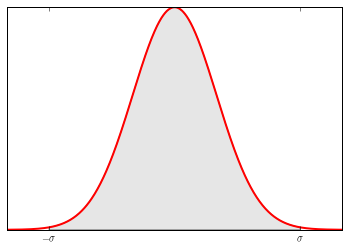
\includegraphics[height=5cm,keepaspectratio=true]{./pe/norm3.png}
 % norm1.png: 0x0 pixel, 300dpi, 0.00x0.00 cm, bb=
 \label{fig:2.10.4}
\end{figure}
\begin{verbatim}
 #(0.9973002039367399, 1.1072256503105314e-14)
\end{verbatim}


 \begin{figure}
 \centering
 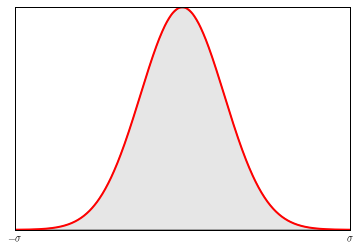
\includegraphics[height=5cm,keepaspectratio=true]{./pe/norm4.png}
 % norm1.png: 0x0 pixel, 300dpi, 0.00x0.00 cm, bb=
 \label{fig:2.10.5}
\end{figure}
\begin{verbatim}
 #(0.9999366575163339, 4.838904125482879e-12)
\end{verbatim}


\lstinputlisting[language=Python]{../code/distribuciones-especiales/normalCDF.py}
\begin{center}
 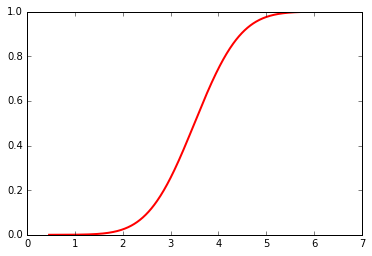
\includegraphics[height=5cm,keepaspectratio=true]{./pe/normCDF.png}
 % normCDF.png: 0x0 pixel, 300dpi, 0.00x0.00 cm, bb=
\end{center}



\subsection{Relación entre las distribuciones binomial y normal}

 Si $N\sim \infty, p,q>>0,$ y $X$ es un distribución binomial con parámetros $N,p$ entonces
 \begin{align}
  \dfrac{X-Np}{\sqrt{Npq}} \sim N(0,1).
 \end{align}



 \begin{ejemplo}
  \label{exmp:2.10.4}
  Consideremos el experimento de lanzar 16 veces una moneda. Repitamos 1,000,000 dicho experimento. Compruebe que dicho experimento se puede modelar por una variable aleatoria con distribución $N(\mu=8,\sigma^{2}=4)$
 \end{ejemplo}


\lstinputlisting[language=Python]{../code/distribuciones-especiales/relBinomNormal.py}
\begin{center}
 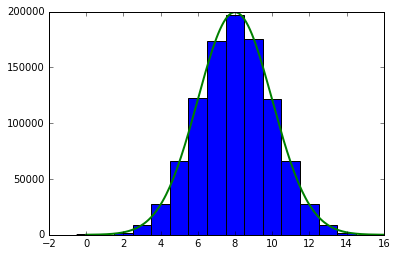
\includegraphics[height=5cm]{./pe/relBinNorm.png}
 % relBinNorm.png: 0x0 pixel, 300dpi, 0.00x0.00 cm, bb=
\end{center}


\subsection{Problemas Resueltos}
{Percentil}
 Diremos que $x=P_{q}$ es el percentil $q, \; 0\leq q \leq 100$ de la distribución $F(x)$ si $F(P_{q})=q\%.$  En el caso de que $q$ sea un valor realizable de $F(x),$ podemos \emph{``despejar''}
 \begin{align}
  P_{q}=F^{-1}\left( \dfrac{q}{100} \right).
 \end{align}
 A tal función se le llama \emph{distribución inversa.}


{Cuartiles}
 En la literatura se definen conceptos similares. Por ejemplo, el primer \emph{cuartil} corresponde al percentil $25;$ el segundo cuartil al percentil $50;$ y así sucesivamente.

{Combinaciones}
 \begin{ejemplo}
  \label{exmp:2.10.7}
  Encuentre
  \begin{enumerate}
   \item $5!$
   \item $\comb{8}{3}$
  \end{enumerate}
  utilizando \texttt{Python.}
 \end{ejemplo}


\lstinputlisting[language=Python]{../code/distribuciones-especiales/combinaciones.py}




{Distribución Binomial}
 \begin{ejemplo}
  \label{exmp:2.10.8}
  Supóngase que $15\%$ de la población es zurda. Encontrar la probabilidad de que en un grupo de 50 individuos haya:
  \begin{enumerate}
   \item cuando mucho 10 zurdos;
   \item por lo menos 5 zurdos;
   \item entre 3 y 6 zurdos;
   \item exactamente 5 zurdos.
  \end{enumerate}

 \end{ejemplo}


\lstinputlisting[language=Python]{../code/distribuciones-especiales/solvedBinom.py}



{Distribución Normal}
 \begin{ejemplo}
  \label{exmp:2.10.9}
  En un examen final de matemáticas, la media fue 72 y la desviación estándar fue 15. Determinar las puntuaciones estándar de los estudiantes que obtuvieron:
  \begin{enumerate}
   \item $60$;
   \item $93$;
   \item $72$.
  \end{enumerate}

 \end{ejemplo}



 \begin{ejemplo}
   \label{exmp:2.10.10}
   Con los datos del problema \ref{exmp:2.10.9}, encontrar las calificaciones que corresponden a las siguientes puntuaciones estándar:
  \begin{enumerate}
   \item $-1$;
   \item $1.6$.
  \end{enumerate}

 \end{ejemplo}



 \begin{ejemplo}
  \label{exmp:2.10.11}
  Supóngase que la cantidad de juegos en que participan los beisbolistas de la liga mayor durante su carrera se distribuye normalmente con media de $1500$ juegos y desviación estándar $350$ juegos. Emplear \texttt{Python} para responder las siguientes preguntas:
  \begin{enumerate}
   \item ¿Qué porcentaje participa en menos de 750 juegos?;
   \item ¿qué porcentaje participa en más de 2000 juegos?;
   \item encontrar el \emph{percentil} $90$ de la cantidad de juegos en los que participan en su carrera.
  \end{enumerate}

 \end{ejemplo}


\lstinputlisting[language=Python]{../code/distribuciones-especiales/solvedNorm.py}


{Eventos raros}
\begin{ejemplo}
\label{exmp:2.10.12}
  Si la probabilidad de que un individuo tenga una reacción adversa por la inyección de determinado suero es $0.001,$ determinar la probabilidad de que de 2000 individuos:
 \begin{enumerate}
  \item exactamente 3;
  \item más de 2
 \end{enumerate}
sufran una reacción adversa.
\end{ejemplo}


\lstinputlisting[language=Python]{../code/distribuciones-especiales/eventosRaros.py}



\section{Distribuciones discretas en ciencia de datos}
\subsection{Distribuciones discretas y su relación con ciencia de datos}

Las distribuciones discretas estudiadas en este capítulo no son solo objetos teóricos: son herramientas fundamentales en el análisis y modelado de datos. A continuación se resumen sus aplicaciones más comunes en ciencia de datos.

\begin{itemize}
 \item \textbf{Distribución binomial:} Se utiliza en pruebas A/B para determinar si existe una diferencia estadísticamente significativa entre dos tasas de conversión. También es la base de muchos modelos de clasificación binaria.

 \item \textbf{Distribución de Poisson:} Modela la frecuencia de eventos raros en un intervalo fijo, como el número de visitas a una página web por minuto, las llamadas a un centro de atención por hora, o los defectos por unidad de producción. Es ampliamente usada en análisis de tráfico y detección de anomalías.

 \item \textbf{Distribución geométrica:} Modela el número de ensayos hasta el primer éxito. En ciencia de datos se aplica en análisis de supervivencia (tiempo hasta la primera conversión), modelado de churn y en el diseño de estrategias de retención.

 \item \textbf{Distribución binomial negativa:} Es una extensión de Poisson que permite modelar datos de conteo con \emph{sobredispersión} (varianza mayor que la media). Es frecuente en datos reales donde la variabilidad excede la predicha por Poisson, por ejemplo en el número de transacciones por cliente o el número de clics por usuario.

 \item \textbf{Distribución hipergeométrica:} Se emplea cuando se trabaja con muestras sin reemplazo de poblaciones finitas, como en auditorías de calidad, muestreo de encuestas, o en pruebas estadísticas exactas como la prueba exacta de Fisher.
\end{itemize}

\begin{ejemplo}
 \label{exmp:2.10.18}
 Se quiere analizar el número de clicks que reciben $100$ anuncios publicitarios en una hora. Los datos observados tienen media $\bar{x}=4.2$ y varianza $s^{2}=8.7$. ¿Es razonable modelar estos datos con una distribución de Poisson?
\end{ejemplo}

\begin{solucion}
	En una distribución de Poisson, la media y la varianza son iguales: $\mu = \sigma^{2} = \lambda$. Como en este caso $s^{2} = 8.7 \gg \bar{x} = 4.2$, los datos presentan \emph{sobredispersión}. Por lo tanto, una distribución de Poisson \emph{no} es adecuada. En su lugar, se recomienda usar una distribución binomial negativa, que permite modelar esta variabilidad adicional.
\end{solucion}

\lstinputlisting[language=Python]{../code/distribuciones-especiales/distDataScience.py}

\begin{figure}
 \centering
 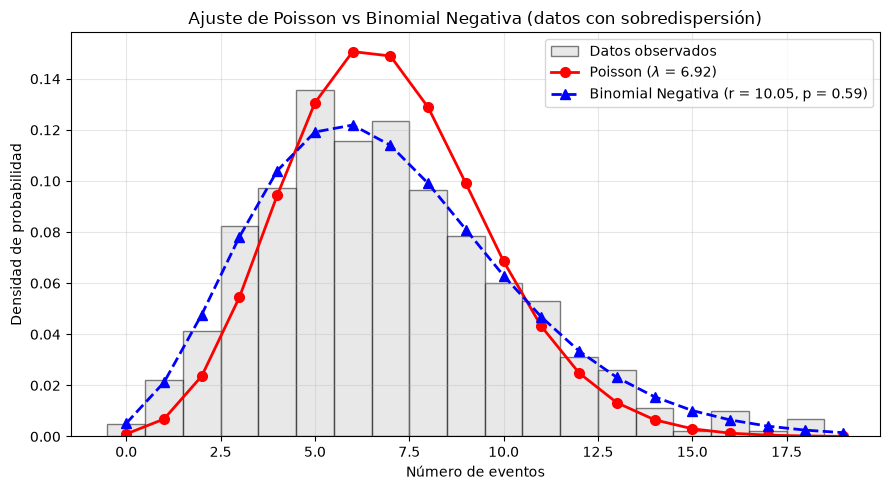
\includegraphics[height=7cm,keepaspectratio=true]{./pe/distDataScience.png}
 % distDataScience.png: 0x0 pixel, 300dpi, 0.00x0.00 cm, bb=
 \caption{Comparación de ajuste de Poisson vs. Binomial Negativa para datos con sobredispersión}
 \label{fig:2.10.10}
\end{figure}

\begin{observacion}
	En la práctica, la elección de la distribución depende tanto de la naturaleza del fenómeno modelado como de las propiedades estadísticas de los datos observados. Herramientas como la función de verosimilitud, el criterio de información de Akaike (AIC) o validación cruzada permiten comparar distintos modelos y elegir el más apropiado.
\end{observacion}



% ==============================================================================
% SECCIÓN 03.04: DISTRIBUCIONES DE BERNOULLI Y BINOMIAL
% ==============================================================================

\subsection*{Enunciados de los problemas --- Sección 03.04}

\subsubsection*{Nivel Fundamental}

\begin{problema}
	\label{prob:3.4.1}
	Considere un experimento aleatorio elemental consistente en la inspección de un único componente electrónico en una línea de montaje, donde la probabilidad de que el componente sea apto para su uso es $p = 0.85$. Sea $X$ la variable aleatoria que toma el valor $1$ si el componente es apto (éxito) y $0$ si resulta defectuoso (fracaso).
	\begin{enumerate}
		\item Especifique formalmente la función de masa de probabilidad $f_X(x)$ utilizando la forma compacta del ensayo de Bernoulli: $f_X(x) = p^x (1-p)^{1-x}$ para $x \in \set{0, 1}$.
		\item Demuestre directamente a partir de la definición que $\mathbb{E}[X] = p$ y $\text{Var}(X) = p(1-p)$.
	\end{enumerate}
\end{problema}

\begin{problema}
	\label{prob:3.4.2}
	En un proceso automático de control de calidad, se inspeccionan $n = 8$ sensores de temperatura fabricados en condiciones idénticas e independientes. La probabilidad de que un sensor individual cumpla con los estándares de precisión es $p = 0.90$. Sea $X$ el número total de sensores que cumplen con los estándares entre los $8$ inspeccionados.
	\begin{enumerate}
		\item Identifique la distribución exacta de $X$ junto con sus parámetros paramétricos y calcule la probabilidad de que exactamente $7$ sensores cumplan con los estándares.
		\item Calcule la probabilidad de que a lo sumo $1$ sensor resulte no apto en la muestra inspeccionada.
	\end{enumerate}
\end{problema}

\begin{problema}
	\label{prob:3.4.3}
	Sea un conjunto de ensayos independientes de Bernoulli $X_1, X_2, \dots, X_n$, donde cada variable aleatoria cumple que $P(X_i = 1) = p$ y $P(X_i = 0) = q = 1-p$ para todo $i \in \set{1, 2, \dots, n}$.
	\begin{enumerate}
		\item Defina la variable sumatoria $Y = \sum_{i=1}^n X_i$. Explique argumentativamente por qué el número de secuencias en el espacio muestral $\Omega$ que producen exactamente $k$ éxitos ($Y = k$) está dado por el coeficiente combinatorio $\comb{n}{k}$.
		\item Utilice este razonamiento para deducir de primeros principios la función de masa de probabilidad $P(Y = k) = \comb{n}{k} p^k q^{n-k}$ y verifique explícitamente su suma sobre el soporte $\mathcal{S}_Y = \set{0, 1, \dots, n}$.
	\end{enumerate}
\end{problema}

\subsubsection*{Nivel Operativo}

\begin{problema}
	\label{prob:3.4.4}
	Una firma de ciberseguridad monitorea una red de servidores donde la probabilidad de que un intento de acceso externo sea clasificado como malicioso es $p = 0.15$. En un intervalo de tiempo dado se registran $n = 12$ intentos de acceso independientes. Sea $X \sim \text{Bin}(12, 0.15)$ el número de accesos maliciosos detectados.
	\begin{enumerate}
		\item Calcule la probabilidad de que se detecten a lo sumo $2$ accesos maliciosos ($P(X \le 2)$).
		\item Calcule la probabilidad condicional de que se detecten al menos $4$ accesos maliciosos dado que se detectó al menos uno ($P(X \ge 4 \mid X \ge 1)$).
	\end{enumerate}
\end{problema}

\begin{problema}
	\label{prob:3.4.5}
	Un equipo de investigación en bioinformática desarrolla un algoritmo para la detección de una secuencia genética rara en muestras clínicas. La probabilidad de que una muestra positiva sea correctamente identificada en un ensayo individual es $p = 0.08$. Si los ensayos se realizan de manera totalmente independiente sobre muestras distintas:
	\begin{enumerate}
		\item Plantee la inecuación logarítmica que permite determinar el número mínimo de muestras independientes $n$ que deben procesarse para que la probabilidad de detectar la secuencia al menos una vez sea de mínimo $99\%$ ($P(X \ge 1) \ge 0.99$).
		\item Resuelva numéricamente para obtener el valor entero exacto de $n^*$.
	\end{enumerate}
\end{problema}

\begin{problema}
	\label{prob:3.4.6}
	Un fabricante de componentes aeroespaciales suministra lotes de $n = 20$ válvulas hidráulicas. La probabilidad de que una válvula defectuosa escape al control interno es $p = 0.05$. El contrato contractual establece un costo operativo de garantía modelado por la función de pérdida no lineal:
	\begin{align*}
		C(X) = 500 X^2 + 150 X + 1000 \quad \text{(en dólares)},
	\end{align*}
	donde $X$ representa el número de válvulas defectuosas en el lote entregado.
	\begin{enumerate}
		\item Determine la esperanza matemática del costo de garantía $\mathbb{E}[C(X)]$ utilizando las propiedades de los momentos binomiales.
		\item Calcule la desviación estándar del número de defectos $\sigma_X$ y discuta el impacto del término cuadrático $X^2$ en el costo esperado global.
	\end{enumerate}
\end{problema}

\subsubsection*{Nivel Analítico}

\begin{problema}
	\label{prob:3.4.7}
	Sea $X \sim \text{Bin}(n, p)$ con $q = 1-p$.
	\begin{enumerate}
		\item Demuestre rigurosamente, utilizando el Teorema del Binomio de Newton, la identidad de normalización absoluta:
		\begin{align*}
			\sum_{k=0}^n \comb{n}{k} p^k q^{n-k} = 1.
		\end{align*}
		\item Aplicando el operador diferencial $\frac{\partial}{\partial p}$ a la identidad analítica $(p+q)^n = \sum_{k=0}^n \comb{n}{k} p^k q^{n-k}$ antes de sustituir $q=1-p$, demuestre analíticamente que $\mathbb{E}[X] = np$.
	\end{enumerate}
\end{problema}

\begin{problema}
	\label{prob:3.4.8}
	Para una variable aleatoria discreta $X \sim \text{Bin}(n, p)$, el segundo momento factorial se define como el valor esperado del producto descendente $\mathbb{E}[X(X-1)]$.
	\begin{enumerate}
		\item Deduzca analíticamente la fórmula cerrada de $\mathbb{E}[X(X-1)]$ manipulando los coeficientes combinatorios de la suma $\sum_{k=2}^n k(k-1)\comb{n}{k} p^k q^{n-k}$.
		\item A partir de la identidad algebraica $\text{Var}(X) = \mathbb{E}[X(X-1)] + \mathbb{E}[X] - (\mathbb{E}[X])^2$, demuestre de forma exacta que $\text{Var}(X) = np(1-p)$.
	\end{enumerate}
\end{problema}

\subsubsection*{Nivel Desafiante}

\begin{problema}
	\label{prob:3.4.9}
	Sea $X \sim \text{Bin}(n, p)$ una variable binomial con probabilidad de éxito $0 < p < 1$. Se define la moda de la distribución como el valor o los valores $k^* \in \set{0, 1, \dots, n}$ que maximizan la probabilidad $P(X = k^*)$.
	\begin{enumerate}
		\item Analice el cociente de probabilidades adyacentes $R(k) = \dfrac{P(X = k)}{P(X = k-1)}$ para todo $k \in \set{1, 2, \dots, n}$.
		\item Demuestre analíticamente que la moda de la distribución cumple que $k^* = \lfloor (n+1)p \rfloor$ cuando $(n+1)p$ no es un número entero.
		\item Determine exactamente qué ocurre con la distribución cuando $(n+1)p = m \in \mathbb{Z}^+$ (caso bimodal).
	\end{enumerate}
\end{problema}

\begin{problema}
	\label{prob:3.4.10}
	Considere dos variables aleatorias binomiales mutuamente independientes: $X \sim \text{Bin}(n_1, p)$ y $Y \sim \text{Bin}(n_2, p)$, ambas compartiendo exactamente la misma probabilidad de éxito $p$ en cada ensayo.
	\begin{enumerate}
		\item Demuestre combinatoriamente, utilizando la convolución discreta y la Identidad de Vandermonde, que la suma $Z = X + Y$ sigue una distribución exacta $\text{Bin}(n_1 + n_2, p)$.
		\item Compruebe que la aditividad de la esperanza y la varianza se conserva de manera exacta bajo esta suma de distribuciones independientes.
	\end{enumerate}
\end{problema}

\subsection*{Sugerencias de los problemas --- Sección 03.04}

\begin{sugerencia}
	\label{sug:3.4.1}
	Para el Problema \ref{prob:3.4.1}, evalúe la expresión compacta $p^x(1-p)^{1-x}$ en $x=0$ y $x=1$ para verificar que coincide con la definición de probabilidad de éxito y fracaso. Para los momentos, aplique la suma directa $\mathbb{E}[X^k] = 0^k \cdot (1-p) + 1^k \cdot p$.
\end{sugerencia}

\begin{sugerencia}
	\label{sug:3.4.2}
	Para el Problema \ref{prob:3.4.2}, recuerde que la condición "a lo sumo $1$ sensor no apto" equivale exactamente a que al menos $7$ sensores cumplan con los estándares ($X \ge 7$), lo cual implica evaluar $P(X=7) + P(X=8)$.
\end{sugerencia}

\begin{sugerencia}
	\label{sug:3.4.3}
	Para el Problema \ref{prob:3.4.3}, cada secuencia particular de $k$ éxitos y $n-k$ fracasos tiene una probabilidad individual de $p^k q^{n-k}$ por independencia. El número total de configuraciones distintas para ubicar los $k$ éxitos en las $n$ posiciones es $\comb{n}{k}$.
\end{sugerencia}

\begin{sugerencia}
	\label{sug:3.4.4}
	Para el Problema \ref{prob:3.4.4}, en la parte condicional utilice la definición de probabilidad condicional: $P(X \ge 4 \mid X \ge 1) = \dfrac{P(X \ge 4 \cap X \ge 1)}{P(X \ge 1)} = \dfrac{1 - P(X \le 3)}{1 - P(X = 0)}$.
\end{sugerencia}

\begin{sugerencia}
	\label{sug:3.4.5}
	Para el Problema \ref{prob:3.4.5}, el evento complementario a "detectar al menos una vez" es "cero detecciones en $n$ ensayos" ($X=0$), cuya probabilidad es exactamente $(1-p)^n$. Exprese la condición como $1 - (1-p)^n \ge 0.99$.
\end{sugerencia}

\begin{sugerencia}
	\label{sug:3.4.6}
	Para el Problema \ref{prob:3.4.6}, por linealidad del operador esperanza, $\mathbb{E}[C(X)] = 500 \mathbb{E}[X^2] + 150 \mathbb{E}[X] + 1000$. Recuerde que el segundo momento bruto se obtiene como $\mathbb{E}[X^2] = \text{Var}(X) + (\mathbb{E}[X])^2 = np(1-p) + n^2 p^2$.
\end{sugerencia}

\begin{sugerencia}
	\label{sug:3.4.7}
	Para el Problema \ref{prob:3.4.7}, al derivar $(p+q)^n$ respecto a $p$ obtenemos $n(p+q)^{n-1}$. Al derivar el lado derecho de la suma obtenemos $\sum k \comb{n}{k} p^{k-1} q^{n-k}$. Multiplique por $p$ a ambos lados y luego sustituya $q = 1-p$.
\end{sugerencia}

\begin{sugerencia}
	\label{sug:3.4.8}
	Para el Problema \ref{prob:3.4.8}, note que para $k \ge 2$, $k(k-1)\comb{n}{k} = n(n-1)\comb{n-2}{k-2}$. Factorice $n(n-1)p^2$ fuera de la suma y reconozca la normalización de una binomial con parámetros $n-2$ y $p$.
\end{sugerencia}

\begin{sugerencia}
	\label{sug:3.4.9}
	Para el Problema \ref{prob:3.4.9}, plantee la condición de crecimiento $R(k) = \dfrac{\comb{n}{k} p^k q^{n-k}}{\comb{n}{k-1} p^{k-1} q^{n-k+1}} = \dfrac{(n-k+1)p}{kq} \ge 1$. Despeje la variable $k$ en función de $(n+1)p$.
\end{sugerencia}

\begin{sugerencia}
	\label{sug:3.4.10}
	Para el Problema \ref{prob:3.4.10}, exprese la masa de probabilidad del suma como $P(Z = m) = \sum_{j=0}^m P(X = j) P(Y = m-j) = \sum_{j=0}^m \comb{n_1}{j}\comb{n_2}{m-j} p^m q^{(n_1+n_2)-m}$. Aplique la Identidad de Vandermonde: $\sum_{j=0}^m \comb{n_1}{j}\comb{n_2}{m-j} = \comb{n_1+n_2}{m}$.
\end{sugerencia}

\subsection*{Soluciones de los problemas --- Sección 03.04}

\begin{solucion}
	\label{sol:3.4.1}
	Para el Problema \ref{prob:3.4.1}:
	\begin{enumerate}
		\item Para el componente electrónico, el soporte discreto es $\mathcal{S}_X = \set{0, 1}$. Evaluar la forma paramétrica compacta arroja:
		\begin{align*}
			f_X(1) &= p^1 (1-p)^{1-1} = p = 0.85, \\
			f_X(0) &= p^0 (1-p)^{1-0} = 1-p = 0.15.
		\end{align*}
		La suma sobre el soporte es $\sum_{x \in \set{0,1}} f_X(x) = p + (1-p) = 1$, confirmando su normalización exacta.
		\item Calculamos el primer momento bruto (esperanza matemática):
		\begin{align*}
			\mathbb{E}[X] &= \sum_{x \in \set{0,1}} x \cdot f_X(x) = 0 \cdot (1-p) + 1 \cdot p = p.
		\end{align*}
		Para el segundo momento bruto, al ser $x^2 = x$ para todo $x \in \set{0, 1}$:
		\begin{align*}
			\mathbb{E}[X^2] &= \sum_{x \in \set{0,1}} x^2 \cdot f_X(x) = 0^2 \cdot (1-p) + 1^2 \cdot p = p.
		\end{align*}
		Por la identidad de König-Huygens, la varianza es:
		\begin{align*}
			\text{Var}(X) &= \mathbb{E}[X^2] - (\mathbb{E}[X])^2 = p - p^2 = p(1-p).
		\end{align*}
		Sustituyendo $p = 0.85$, obtenemos $\mathbb{E}[X] = 0.85$ y $\text{Var}(X) = 0.85 \times 0.15 = 0.1275$.
	\end{enumerate}
\end{solucion}

\begin{solucion}
	\label{sol:3.4.2}
	Para el Problema \ref{prob:3.4.2}:
	\begin{enumerate}
		\item La variable aleatoria que cuenta éxitos independientes entre un número fijo de ensayos sigue una distribución binomial: $X \sim \text{Bin}(n=8, p=0.90)$. La probabilidad exacta de obtener $7$ sensores aptos es:
		\begin{align*}
			P(X = 7) &= \comb{8}{7} (0.90)^7 (0.10)^{8-7} \\
			&= 8 \times 0.4782969 \times 0.10 \approx 0.3826.
		\end{align*}
		\item Que haya a lo sumo $1$ sensor no apto significa que el número de sensores defectuosos ($8-X$) es $\le 1$, lo cual ocurre si y solo si los sensores aptos son exactamente $7$ u $8$:
		\begin{align*}
			P(X \ge 7) &= P(X = 7) + P(X = 8) \\
			&= 0.38263752 + \comb{8}{8} (0.90)^8 (0.10)^0 \\
			&= 0.38263752 + 1 \times 0.43046721 \approx 0.8131.
		\end{align*}
		Existe un $81.31\%$ de probabilidad de que el lote inspeccionado tenga a lo sumo un fallo.
	\end{enumerate}
\end{solucion}

\begin{solucion}
	\label{sol:3.4.3}
	Para el Problema \ref{prob:3.4.3}:
	\begin{enumerate}
		\item El espacio muestral completo del experimento consta de $2^n$ secuencias ordenadas de ceros y unos de la forma $\omega = (x_1, x_2, \dots, x_n)$. Como cada variable es independiente, la probabilidad de cualquier secuencia particular que contenga exactamente $k$ unos (éxitos) y $n-k$ ceros (fracasos) está dada por el producto de sus probabilidades marginales:
		\begin{align*}
			P(\omega) &= \prod_{i=1}^n P(X_i = x_i) = p^k q^{n-k}.
		\end{align*}
		El número total de secuencias en $\Omega$ que contienen exactamente $k$ éxitos es el problema combinatorio de elegir las $k$ posiciones de los éxitos entre los $n$ lugares disponibles, lo cual es el coeficiente combinatorio $\comb{n}{k} = \dfrac{n!}{k!(n-k)!}$.
		\item Dado que las secuencias que producen $Y=k$ son eventos mutuamente excluyentes y equiprobables entre sí con probabilidad $p^k q^{n-k}$, sumando sobre las $\comb{n}{k}$ configuraciones obtenemos la función de masa de probabilidad binomial:
		\begin{align*}
			P(Y = k) = \comb{n}{k} p^k q^{n-k}, \quad k \in \set{0, 1, \dots, n}.
		\end{align*}
		Su suma sobre todo el soporte $\mathcal{S}_Y$ es:
		\begin{align*}
			\sum_{k=0}^n P(Y = k) = \sum_{k=0}^n \comb{n}{k} p^k q^{n-k} = (p + q)^n = 1^n = 1,
		\end{align*}
		lo cual confirma que es una función de masa de probabilidad matemáticamente completa.
	\end{enumerate}
\end{solucion}

\begin{solucion}
	\label{sol:3.4.4}
	Para el Problema \ref{prob:3.4.4}:
	\begin{enumerate}
		\item Con $X \sim \text{Bin}(12, 0.15)$, calculamos las probabilidades acumuladas hasta $k=2$:
		\begin{align*}
			P(X = 0) &= \comb{12}{0} (0.15)^0 (0.85)^{12} = (0.85)^{12} \approx 0.14224, \\
			P(X = 1) &= \comb{12}{1} (0.15)^1 (0.85)^{11} = 12 \times 0.15 \times 0.16734 \approx 0.30121, \\
			P(X = 2) &= \comb{12}{2} (0.15)^2 (0.85)^{10} = 66 \times 0.0225 \times 0.19687 \approx 0.29236.
		\end{align*}
		Sumando las tres probabilidades elementales:
		\begin{align*}
			P(X \le 2) = 0.14224 + 0.30121 + 0.29236 = 0.7358.
		\end{align*}
		\item Para la probabilidad condicional de al menos $4$ detecciones dado al menos una, calculamos primero $P(X = 3)$:
		\begin{align*}
			P(X = 3) &= \comb{12}{3} (0.15)^3 (0.85)^9 = 220 \times 0.003375 \times 0.23162 \approx 0.17197.
		\end{align*}
		Por lo tanto, la probabilidad de tener $3$ o menos detecciones es $P(X \le 3) = 0.73581 + 0.17197 = 0.90778$. La probabilidad condicional requerida es:
		\begin{align*}
			P(X \ge 4 \mid X \ge 1) &= \dfrac{P(X \ge 4 \cap X \ge 1)}{P(X \ge 1)} = \dfrac{P(X \ge 4)}{P(X \ge 1)} = \dfrac{1 - P(X \le 3)}{1 - P(X = 0)} \\
			&= \dfrac{1 - 0.90778}{1 - 0.14224} = \dfrac{0.09222}{0.85776} \approx 0.1075.
		\end{align*}
	\end{enumerate}
\end{solucion}

\begin{solucion}
	\label{sol:3.4.5}
	Para el Problema \ref{prob:3.4.5}:
	\begin{enumerate}
		\item Sea $X \sim \text{Bin}(n, p=0.08)$ el número de secuencias detectadas. Queremos garantizar que:
		\begin{align*}
			P(X \ge 1) \ge 0.99.
		\end{align*}
		Utilizando el evento complementario, $P(X \ge 1) = 1 - P(X = 0) = 1 - (1-p)^n = 1 - (0.92)^n$. Sustituyendo en la desigualdad:
		\begin{align*}
			1 - (0.92)^n \ge 0.99 \implies (0.92)^n \le 0.01.
		\end{align*}
		Aplicando logaritmo natural (y dado que $\ln(0.92) < 0$, el signo de la desigualdad se invierte):
		\begin{align*}
			n \cdot \ln(0.92) \le \ln(0.01) \implies n \ge \dfrac{\ln(0.01)}{\ln(0.92)}.
		\end{align*}
		\item Evaluando los logaritmos numéricamente con alta precisión:
		\begin{align*}
			\ln(0.01) \approx -4.605170, \quad \ln(0.92) \approx -0.083382.
		\end{align*}
		El cociente exacto es:
		\begin{align*}
			n \ge \dfrac{-4.605170}{-0.083382} \approx 55.2299.
		\end{align*}
		Como el tamaño de muestra $n$ debe ser un número entero positivo, aplicamos la función techo:
		\begin{align*}
			n^* = \lceil 55.2299 \rceil = 56.
		\end{align*}
		Se requieren exactamente $56$ muestras independientes para asegurar el nivel de detección deseado.
	\end{enumerate}
\end{solucion}

\begin{solucion}
	\label{sol:3.4.6}
	Para el Problema \ref{prob:3.4.6}:
	\begin{enumerate}
		\item Para $X \sim \text{Bin}(n=20, p=0.05)$, calculamos primero la media $\mathbb{E}[X]$ y la varianza $\text{Var}(X)$:
		\begin{align*}
			\mathbb{E}[X] &= np = 20 \times 0.05 = 1.0, \\
			\text{Var}(X) &= np(1-p) = 20 \times 0.05 \times 0.95 = 0.95.
		\end{align*}
		El segundo momento bruto es $\mathbb{E}[X^2] = \text{Var}(X) + (\mathbb{E}[X])^2 = 0.95 + (1.0)^2 = 1.95$. Aplicando linealidad al costo de garantía $C(X)$:
		\begin{align*}
			\mathbb{E}[C(X)] &= 500 \mathbb{E}[X^2] + 150 \mathbb{E}[X] + 1000 \\
			&= 500(1.95) + 150(1.0) + 1000 = 975 + 150 + 1000 = \$2,125.
		\end{align*}
		\item La desviación estándar del número de componentes defectuosos en el lote es:
		\begin{align*}
			\sigma_X = \sqrt{\text{Var}(X)} = \sqrt{0.95} \approx 0.9747.
		\end{align*}
		Si el costo fuera puramente lineal en la media ($150 \mathbb{E}[X] + 1000$), el costo esperado sería de $\$1,150$. Sin embargo, la no linealidad cuadrática ($500 X^2$) penaliza fuertemente la variabilidad inherente del lote: aun cuando el número promedio de fallas es solo una unidad ($\mu=1$), la dispersión intrínseca agrega un costo esperado de $500 \times 1.95 = \$975$, lo cual representa el $45.88\%$ del costo global.
	\end{enumerate}
\end{solucion}

\begin{solucion}
	\label{sol:3.4.7}
	Para el Problema \ref{prob:3.4.7}:
	\begin{enumerate}
		\item El Teorema del Binomio de Newton establece que para cualquier par de números reales $a, b \in \mathbb{R}$ y entero positivo $n \in \mathbb{Z}^+$:
		\begin{align*}
			(a + b)^n = \sum_{k=0}^n \comb{n}{k} a^k b^{n-k}.
		\end{align*}
		Sustituyendo directamente $a = p$ y $b = q$, obtenemos el lado derecho idéntico a la suma total de probabilidades de la función de masa binomial:
		\begin{align*}
			\sum_{k=0}^n \comb{n}{k} p^k q^{n-k} = (p + q)^n.
		\end{align*}
		Como por definición de probabilidad de fracaso se cumple que $p + q = 1$, la expresión se reduce a $1^n = 1$, demostrando formalmente la normalización absoluta.
		\item Tratando a $p$ y $q$ como variables independientes en la identidad general $(p+q)^n = \sum_{k=0}^n \comb{n}{k} p^k q^{n-k}$ y aplicando el operador diferencial respecto a $p$:
		\begin{align*}
			\dfrac{\partial}{\partial p} (p+q)^n &= \sum_{k=0}^n \comb{n}{k} \dfrac{\partial}{\partial p} (p^k q^{n-k}) \\
			n(p+q)^{n-1} &= \sum_{k=1}^n k \comb{n}{k} p^{k-1} q^{n-k}.
		\end{align*}
		Multiplicamos ambos lados de la ecuación por el parámetro $p$:
		\begin{align*}
			np(p+q)^{n-1} = \sum_{k=1}^n k \comb{n}{k} p^k q^{n-k} = \sum_{k=0}^n k \comb{n}{k} p^k q^{n-k}.
		\end{align*}
		El lado derecho de esta ecuación coincide exactamente con la definición analítica del valor esperado $\mathbb{E}[X] = \sum_{k=0}^n k P(X = k)$. Al sustituir la condición geométrica $q = 1-p \implies p+q=1$ en el lado izquierdo, concluimos la demostración:
		\begin{align*}
			\mathbb{E}[X] = np(1)^{n-1} = np.
		\end{align*}
	\end{enumerate}
\end{solucion}

\begin{solucion}
	\label{sol:3.4.8}
	Para el Problema \ref{prob:3.4.8}:
	\begin{enumerate}
		\item Evaluamos la definición formal de segundo momento factorial $\mathbb{E}[X(X-1)]$:
		\begin{align*}
			\mathbb{E}[X(X-1)] &= \sum_{k=0}^n k(k-1) P(X = k) = \sum_{k=2}^n k(k-1) \comb{n}{k} p^k q^{n-k}.
		\end{align*}
		Desarrollamos el coeficiente combinatorio y cancelamos los factores algebraicos:
		\begin{align*}
			k(k-1) \comb{n}{k} &= k(k-1) \dfrac{n!}{k!(n-k)!} = \dfrac{n!}{(k-2)!(n-k)!} \\
			&= n(n-1) \dfrac{(n-2)!}{(k-2)!((n-2)-(k-2))!} = n(n-1) \comb{n-2}{k-2}.
		\end{align*}
		Sustituyendo este desarrollo combinatorio en la sumatoria y factorizando $n(n-1)p^2$:
		\begin{align*}
			\mathbb{E}[X(X-1)] &= \sum_{k=2}^n n(n-1)\comb{n-2}{k-2} p^2 p^{k-2} q^{(n-2)-(k-2)} \\
			&= n(n-1)p^2 \sum_{j=0}^{n-2} \comb{n-2}{j} p^j q^{(n-2)-j}, \quad \text{donde } j = k-2.
		\end{align*}
		Por el Teorema del Binomio demostrado previamente, la sumatoria interna vale exactamente $(p+q)^{n-2} = 1$. Por lo tanto:
		\begin{align*}
			\mathbb{E}[X(X-1)] = n(n-1)p^2.
		\end{align*}
		\item Desarrollamos el momento factorial relacionándolo con la varianza de la distribución:
		\begin{align*}
			\mathbb{E}[X(X-1)] &= \mathbb{E}[X^2 - X] = \mathbb{E}[X^2] - \mathbb{E}[X] \\
			\implies \mathbb{E}[X^2] &= \mathbb{E}[X(X-1)] + \mathbb{E}[X].
		\end{align*}
		Sustituyendo $\mathbb{E}[X(X-1)] = n(n-1)p^2$ y $\mathbb{E}[X] = np$, obtenemos el segundo momento bruto:
		\begin{align*}
			\mathbb{E}[X^2] = n(n-1)p^2 + np = n^2 p^2 - np^2 + np.
		\end{align*}
		Finalmente, calculamos la varianza operacional:
		\begin{align*}
			\text{Var}(X) &= \mathbb{E}[X^2] - (\mathbb{E}[X])^2 = (n^2 p^2 - np^2 + np) - (np)^2 \\
			&= np - np^2 = np(1-p),
		\end{align*}
		concluyendo la deducción de la varianza binomial de manera exacta.
	\end{enumerate}
\end{solucion}

\begin{solucion}
	\label{sol:3.4.9}
	Para el Problema \ref{prob:3.4.9}:
	\begin{enumerate}
		\item Para determinar dónde alcanza su máximo la función de masa binomial, investigamos cuándo la probabilidad crece de un término al siguiente ($P(X=k) \ge P(X=k-1)$). Evaluamos el cociente adyacente $R(k)$:
		\begin{align*}
			R(k) = \dfrac{P(X=k)}{P(X=k-1)} &= \dfrac{\comb{n}{k} p^k q^{n-k}}{\comb{n}{k-1} p^{k-1} q^{n-k+1}} = \dfrac{\dfrac{n!}{k!(n-k)!}}{\dfrac{n!}{(k-1)!(n-k+1)!}} \cdot \dfrac{p}{q} \\
			&= \dfrac{(k-1)!(n-k+1)!}{k!(n-k)!} \cdot \dfrac{p}{q} = \dfrac{n-k+1}{k} \cdot \dfrac{p}{1-p}.
		\end{align*}
		\item La probabilidad binomial es creciente en el paso $k$ si y solo si $R(k) \ge 1$:
		\begin{align*}
			\dfrac{n-k+1}{k} \cdot \dfrac{p}{1-p} \ge 1 &\implies (n-k+1)p \ge k(1-p) \\
			&\implies np - kp + p \ge k - kp \\
			&\implies (n+1)p \ge k.
		\end{align*}
		Por lo tanto, las probabilidades son estrictamente crecientes en los enteros $k$ tales que $k \le (n+1)p$, y estrictamente decrecientes para los enteros $k > (n+1)p$. Cuando la cantidad $(n+1)p$ no es un número entero, existe un único número entero $k^*$ que satisface la condición de máximo, el cual se obtiene tomando la parte entera inferior:
		\begin{align*}
			k^* = \lfloor (n+1)p \rfloor.
		\end{align*}
		\item Si el valor admisible $(n+1)p = m$ resulta ser un entero positivo exacto, entonces en el punto de transición $k = m$ se tiene una igualdad en el cociente adyacente:
		\begin{align*}
			R(m) = 1 \implies P(X = m) = P(X = m-1).
		\end{align*}
		En este caso extraordinario la distribución es exactamente **bimodal**, alcanzando su máximo valor idéntico en dos puntos enteros contiguos del soporte: $k^* = m-1$ y $k^* = m$.
	\end{enumerate}
\end{solucion}

\begin{solucion}
	\label{sol:3.4.10}
	Para el Problema \ref{prob:3.4.10}:
	\begin{enumerate}
		\item Al ser $X$ y $Y$ independientes con el mismo éxito $p$, la probabilidad de que la suma tome un valor entero $Z = X+Y = m$ para $m \in \set{0, 1, \dots, n_1+n_2}$ se obtiene mediante la fórmula de convolución discreta:
		\begin{align*}
			P(Z = m) &= \sum_{j=0}^m P(X = j \cap Y = m-j) = \sum_{j=0}^m P(X = j)P(Y = m-j) \\
			&= \sum_{j=0}^m \left[ \comb{n_1}{j} p^j q^{n_1-j} \right] \left[ \comb{n_2}{m-j} p^{m-j} q^{n_2-(m-j)} \right] \\
			&= p^m q^{(n_1+n_2)-m} \sum_{j=0}^m \comb{n_1}{j} \comb{n_2}{m-j}.
		\end{align*}
		La sumatoria combinatoria remanente se resuelve mediante la célebre **Identidad combinatoria de Vandermonde**, la cual establece que al seleccionar un subconjunto de tamaño $m$ de un grupo combinado de $n_1 + n_2$ elementos divididos en dos subgrupos disjuntos:
		\begin{align*}
			\sum_{j=0}^m \comb{n_1}{j} \comb{n_2}{m-j} = \comb{n_1+n_2}{m}.
		\end{align*}
		Sustituyendo la Identidad de Vandermonde en la convolución, obtenemos de forma cerrada:
		\begin{align*}
			P(Z = m) = \comb{n_1+n_2}{m} p^m q^{(n_1+n_2)-m},
		\end{align*}
		lo que demuestra que $Z \sim \text{Bin}(n_1+n_2, p)$.
		\item Verificamos la aditividad de momentos sobre la suma binomial:
		\begin{align*}
			\mathbb{E}[Z] &= (n_1 + n_2)p = n_1 p + n_2 p = \mathbb{E}[X] + \mathbb{E}[Y], \\
			\text{Var}(Z) &= (n_1 + n_2)p(1-p) = n_1 p(1-p) + n_2 p(1-p) = \text{Var}(X) + \text{Var}(Y).
		\end{align*}
		El teorema combinatorio y aditivo queda rigurosamente demostrado.
	\end{enumerate}
\end{solucion}

% ==============================================================================
% SECCIÓN 03.05: DISTRIBUCIONES GEOMÉTRICA Y BINOMIAL NEGATIVA
% ==============================================================================

\subsection*{Enunciados de los problemas --- Sección 03.05}

\subsubsection*{Nivel Fundamental}

\begin{problema}
	\label{prob:3.5.1}
	Considere una secuencia infinita de ensayos de Bernoulli independientes con probabilidad constante de éxito $p \in (0, 1)$ en cada intento y probabilidad de fracaso $q = 1-p$. Sea $X$ la variable aleatoria discreta que denota el número total de ensayos requeridos hasta obtener el **primer éxito** (incluyendo el ensayo exitoso).
	\begin{enumerate}
		\item Especifique la función de masa de probabilidad $f_X(k) = P(X = k)$ y determine su soporte $\mathcal{S}_X$.
		\item Demuestre analíticamente que la suma sobre todo el soporte es igual a la unidad ($\sum_{k=1}^{\infty} f_X(k) = 1$) mediante series geométricas.
		\item Calcule la probabilidad de cola superior $P(X > k)$ para un entero $k \ge 1$ y obtenga una expresión cerrada para la función de distribución acumulada $F_X(k) = P(X \le k)$.
	\end{enumerate}
\end{problema}

\begin{problema}
	\label{prob:3.5.2}
	En un servidor de base de datos de alta concurrencia, las transacciones independientes experimentan fallas de bloqueo por concurrencia con probabilidad constante $p = 0.04$. Sea $X$ el número de intentos necesarios para que una transacción compleja logre ejecutarse con éxito por primera vez.
	\begin{enumerate}
		\item Calcule la probabilidad exacta de que la transacción requiera a lo sumo $3$ intentos para ejecutarse exitosamente.
		\item Si la transacción ya ha fallado en sus primeros $5$ intentos, ¿cuál es la probabilidad condicional de que requiera más de $8$ intentos en total para tener éxito ($P(X > 8 \mid X > 5)$)?
		\item Compare el resultado condicional anterior con la probabilidad no condicional de requerir más de $3$ intentos ($P(X > 3)$) e interprete el resultado en términos de la propiedad intrínseca del proceso.
	\end{enumerate}
\end{problema}

\begin{problema}
	\label{prob:3.5.3}
	Una firma de auditoría contable inspecciona transacciones corporativas de manera secuencial e independiente. Históricamente, se sabe que una fracción $p = 0.10$ de las transacciones presenta alguna irregularidad fiscal. Los auditores deciden continuar inspeccionando hasta encontrar **exactamente $r = 3$ transacciones irregulares**. Sea $X$ el número total de transacciones inspeccionadas.
	\begin{enumerate}
		\item Argumente por qué la probabilidad de que la tercera irregularidad sea detectada exactamente en la vigésima inspección ($X = 20$) adopta la forma combinatoria $P(X = 20) = \comb{19}{2} (0.10)^3 (0.90)^{17}$.
		\item Escriba la función de masa general para $X \sim \text{BN}(r, p)$ sobre su soporte $\mathcal{S}_X = \set{r, r+1, \dots}$.
	\end{enumerate}
\end{problema}

\subsubsection*{Nivel Operativo}

\begin{problema}
	\label{prob:3.5.4}
	En una línea de soldadura láser automatizada para componentes de automoción, los defectos críticos ocurren de manera independiente con probabilidad $p = 0.02$ por pieza. Por protocolo de seguridad industrial, la línea se detiene para un recalibrado mayor en el instante exacto en que se detecta la **cuarta pieza defectuosa** ($r = 4$). Sea $X$ el número total de piezas producidas hasta el paro de la línea.
	\begin{enumerate}
		\item Calcule el número esperado de piezas producidas hasta el recalibrado ($\mathbb{E}[X]$) y la desviación estándar de la producción ($\sigma_X$).
		\item Calcule la probabilidad de que la línea de soldadura logre producir al menos $100$ piezas antes de ser detenida por el cuarto defecto ($P(X \ge 100)$).
	\end{enumerate}
\end{problema}

\begin{problema}
	\label{prob:3.5.5}
	Un equipo de biotecnología realiza microinyecciones en ovocitos de ratón para desarrollar un modelo transgénico. La probabilidad de éxito de cada microinyección es un parámetro desconocido $p \in (0, 1)$. El equipo planea inyectar ovocitos uno tras otro hasta obtener exactamente $r = 5$ embriones viables. Suponga que en el experimento real, el quinto embrión viable se obtuvo exactamente en la microinyección número $25$ ($X = 25$).
	\begin{enumerate}
		\item Escriba la función de verosimilitud $L(p \mid X = 25)$ basada en la distribución Binomial Negativa.
		\item Calcule el estimador de máxima verosimilitud $\hat{p}_{\text{MLE}}$ para la probabilidad de viabilidad e interprete su relación intuitiva con la proporción observada de éxitos.
	\end{enumerate}
\end{problema}

\begin{problema}
	\label{prob:3.5.6}
	Un ingeniero en telecomunicaciones analiza el número de reintentos de conexión por usuario en una hora punta del servidor central. Al ajustar el número de fallas previas al primer éxito con un modelo discreto, observa que la media muestral es $\bar{x} = 3.2$ fallas y la varianza muestral es $s^2 = 13.44$.
	\begin{enumerate}
		\item Explique teóricamente por qué un modelo de distribución de Poisson pura resulta estructuralmente inadecuado para modelar este tráfico de reintentos.
		\item Si se modela el número de fallas $Y = X - r \sim \text{BN}(r, p)$ (donde $Y \in \set{0, 1, \dots}$ tiene media $\mu_Y = \frac{rq}{p}$ y varianza $\sigma_Y^2 = \frac{rq}{p^2}$), utilice el método de momentos igualando $\mu_Y = 3.2$ y $\sigma_Y^2 = 13.44$ para estimar los parámetros poblacionales $\hat{p}$ y $\hat{r}$.
	\end{enumerate}
\end{problema}

\subsubsection*{Nivel Analítico}

\begin{problema}
	\label{prob:3.5.7}
	Sea un experimento secuencial donde $X \sim \text{BN}(r, p)$ cuenta el número total de ensayos de Bernoulli necesarios para acumular $r$ éxitos independientes.
	\begin{enumerate}
		\item Demuestre rigurosamente por descomposición estocástica que $X$ puede expresarse como la suma de $r$ variables aleatorias geométricas independientes e idénticamente distribuidas ($X = \sum_{i=1}^r Y_i$, donde $Y_i \sim \text{Geom}(p)$).
		\item Demuestre por diferenciación de series de potencias que para una única variable $Y_1 \sim \text{Geom}(p)$, la función generadora de momentos es $M_{Y_1}(t) = \dfrac{p e^t}{1 - q e^t}$ para $t < -\ln(q)$.
		\item Utilizando la propiedad de independencia, deduzca la función generadora de momentos $M_X(t)$ de la distribución Binomial Negativa.
	\end{enumerate}
\end{problema}

\begin{problema}
	\label{prob:3.5.8}
	Utilizando las propiedades analíticas del operador diferencial sobre series formales de potencias o la función generadora de momentos $M_X(t) = \left(\dfrac{p e^t}{1 - q e^t}\right)^r$ obtenida en el Problema \ref{prob:3.5.7}:
	\begin{enumerate}
		\item Demuestre de manera exacta que la esperanza matemática del número total de ensayos en una Binomial Negativa es $\mathbb{E}[X] = \dfrac{r}{p}$.
		\item Demuestre algebraicamente que la varianza está dada por $\text{Var}(X) = \dfrac{r q}{p^2} = \dfrac{r(1-p)}{p^2}$.
	\end{enumerate}
\end{problema}

\subsubsection*{Nivel Desafiante}

\begin{problema}
	\label{prob:3.5.9}
	Se afirma que la distribución geométrica es la **única distribución discreta con soporte en los enteros positivos $\mathbb{Z}^+$** que posee la propiedad de pérdida de memoria. Demuestre formalmente este teorema de caracterización:
	\begin{align*}
		P(X > m+n \mid X > m) = P(X > n) \quad \forall m, n \in \mathbb{Z}^+ \iff X \sim \text{Geom}(p).
	\end{align*}
\end{problema}

\begin{problema}
	\label{prob:3.5.10}
	Considere la parametrización del número de fracasos observados antes de obtener $r$ éxitos: $Y = X - r \sim \text{BN}(r, p)$ con soporte $Y \in \set{0, 1, 2, \dots}$ y función de masa $P(Y = y) = \comb{y+r-1}{y} p^r (1-p)^y$. Suponga que el requisito de éxitos crece ilimitadamente ($r \to \infty$) mientras que la probabilidad de éxito de cada ensayo individual tiende a la certeza ($p \to 1$), de tal forma que el número medio esperado de fracasos se mantiene constante e igual a una tasa fija $\lambda > 0$. Esto es, $(1-p)r = \lambda \implies 1-p = \frac{\lambda}{r}$.
	\begin{enumerate}
		\item Demuestre analíticamente mediante límites combinatorios y exponenciales que para cualquier entero no negativo fijo $y \in \set{0, 1, \dots}$:
		\begin{align*}
			\lim_{r \to \infty} P(Y = y) = \dfrac{\lambda^y e^{-\lambda}}{y!}.
		\end{align*}
		\item Interprete físicamente este límite en el contexto del modelado de fenómenos raros y la transición del esquema combinatorio de Pascal al proceso puntual de Poisson.
	\end{enumerate}
\end{problema}

% ------------------------------------------------------------------------------
% SUGERENCIAS --- SECCIÓN 03.05
% ------------------------------------------------------------------------------

\subsection*{Sugerencias de los problemas --- Sección 03.05}

\begin{sugerencia}
	\label{sug:3.5.1}
	Para la suma en el soporte, recuerde la serie geométrica infinita $\sum_{k=0}^{\infty} x^k = \frac{1}{1-x}$ válida cuando $|x| < 1$. Para la cola superior $P(X > k)$, sume la serie desde $j = k+1$ hasta $\infty$ factorizando la potencia común $q^k$.
\end{sugerencia}

\begin{sugerencia}
	\label{sug:3.5.2}
	Exprese la probabilidad condicional utilizando la definición básica: $P(A \mid B) = \frac{P(A \cap B)}{P(B)}$. Note que el evento $\set{X > m+n} \cap \set{X > m}$ es simplemente $\set{X > m+n}$. Sustituya $P(X > j) = q^j$ deducido en el Problema \ref{prob:3.5.1}.
\end{sugerencia}

\begin{sugerencia}
	\label{sug:3.5.3}
	Para que el $r$-ésimo éxito ocurra en el intento exacto $k$, deben cumplirse dos condiciones simultáneas e independientes: (1) haber acumulado exactamente $r-1$ éxitos en los primeros $k-1$ intentos, y (2) que el intento $k$ sea un éxito. Multiplique ambas probabilidades combinando la Binomial y Bernoulli.
\end{sugerencia}

\begin{sugerencia}
	\label{sug:3.5.4}
	Aplique las fórmulas teóricas de momentos de la Binomial Negativa: $\mathbb{E}[X] = \frac{r}{p}$ y $\text{Var}(X) = \frac{rq}{p^2}$. Para la probabilidad $P(X \ge 100)$, reconozca la equivalencia con el conteo binomial: necesitar al menos $100$ ensayos para lograr $4$ defectos equivale a observar a lo sumo $3$ defectos en los primeros $99$ ensayos fabricados.
\end{sugerencia}

\begin{sugerencia}
	\label{sug:3.5.5}
	Tome el logaritmo natural de la verosimilitud $\ln L(p) = \ln \comb{k-1}{r-1} + r \ln(p) + (k-r)\ln(1-p)$. Derive respecto a $p$, iguale a cero y despeje $p$ en términos de $r$ y $k$.
\end{sugerencia}

\begin{sugerencia}
	\label{sug:3.5.6}
	Recuerde que en una distribución de Poisson pura $\mu = \sigma^2$. Para el sistema de ecuaciones con $\text{BN}$, observe el cociente $\frac{\sigma_Y^2}{\mu_Y} = \frac{rq/p^2}{rq/p} = \frac{1}{p} = 1 + \frac{q}{p}$. Despeje $p$ del cociente varianza-media y luego sustitúyalo en $\mu_Y$ para obtener $r$.
\end{sugerencia}

\begin{sugerencia}
	\label{sug:3.5.7}
	El tiempo hasta el $r$-ésimo éxito es la suma del tiempo hasta el 1er éxito ($Y_1$), más el tiempo adicional entre el 1er y el 2do éxito ($Y_2$), y así sucesivamente hasta $Y_r$. Para la FGM, sume la serie $\sum_{k=1}^{\infty} e^{tk} q^{k-1} p$ reescribiéndola como $p e^t \sum_{j=0}^{\infty} (q e^t)^j$.
\end{sugerencia}

\begin{sugerencia}
	\label{sug:3.5.8}
	Puede derivar $M_X(t) = \left(\frac{p e^t}{1-qe^t}\right)^r$ una y dos veces respecto a $t$ y evaluar en $t=0$, o de manera más ágil, aprovechar la independencia y linealidad de momentos proveniente de $X = \sum_{i=1}^r Y_i$ usando los momentos de la geométrica elemental.
\end{sugerencia}

\begin{sugerencia}
	\label{sug:3.5.9}
	Defina la función de cola discreta $G(k) = P(X > k)$. La hipótesis de pérdida de memoria se traduce en la ecuación funcional discreta $G(m+n) = G(m)G(n)$ para todo $m, n \ge 1$. Por inducción sobre $n$, demuestre que $G(n) = [G(1)]^n$ y relacione $G(1)$ con la probabilidad de fracaso $q = 1-p$.
\end{sugerencia}

\begin{sugerencia}
	\label{sug:3.5.10}
	Sustituya $p = 1 - \frac{\lambda}{r}$ en la PMF binomial negativa. Expanda el coeficiente combinatorio $\comb{y+r-1}{y} = \frac{(r+y-1)(r+y-2)\cdots r}{y!}$ y agrupe los $y$ términos que crecen con $r$. Utilice el límite exponencial fundamental $\lim_{r\to\infty} \left(1 - \frac{\lambda}{r}\right)^r = e^{-\lambda}$.
\end{sugerencia}

% ------------------------------------------------------------------------------
% SOLUCIONES --- SECCIÓN 03.05
% ------------------------------------------------------------------------------

\subsection*{Soluciones de los problemas --- Sección 03.05}

\begin{solucion}
	\label{sol:3.5.1}
	Para el Problema \ref{prob:3.5.1}:
	\begin{enumerate}
		\item Para que el primer éxito ocurra exactamente en el ensayo $k \ge 1$, los primeros $k-1$ ensayos debieron resultar en fracasos consecutivos (probabilidad $q^{k-1}$ por independencia mutua) y el ensayo $k$ debe ser un éxito (probabilidad $p$). Por lo tanto:
		\begin{align*}
			f_X(k) = P(X = k) = q^{k-1}p = (1-p)^{k-1}p, \quad \text{para } k \in \mathcal{S}_X = \set{1, 2, 3, \dots}.
		\end{align*}
		\item Sumamos la probabilidad sobre todo el soporte de números enteros positivos:
		\begin{align*}
			\sum_{k=1}^{\infty} f_X(k) &= \sum_{k=1}^{\infty} q^{k-1}p = p \sum_{j=0}^{\infty} q^j, \quad \text{haciendo el cambio de índice } j = k-1.
		\end{align*}
		Como $p \in (0, 1)$, se tiene $q = 1-p \in (0, 1)$. Aplicando la suma exacta de la serie geométrica convergente:
		\begin{align*}
			\sum_{j=0}^{\infty} q^j = \dfrac{1}{1 - q} = \dfrac{1}{1 - (1-p)} = \dfrac{1}{p}.
		\end{align*}
		Sustituyendo en la sumatoria original, obtenemos $p \cdot \dfrac{1}{p} = 1$, lo que demuestra la normalización absoluta de la distribución.
		\item La probabilidad de cola superior $P(X > k)$ representa el evento de que los primeros $k$ intentos sean todos fracasos continuos. Sumando la serie analítica:
		\begin{align*}
			P(X > k) &= \sum_{j=k+1}^{\infty} q^{j-1}p = p q^k \sum_{m=0}^{\infty} q^m = p q^k \left(\dfrac{1}{1-q}\right) = p q^k \left(\dfrac{1}{p}\right) = q^k.
		\end{align*}
		Por complementariedad, la función de distribución acumulada para cualquier entero $k \ge 1$ es:
		\begin{align*}
			F_X(k) = P(X \le k) = 1 - P(X > k) = 1 - q^k = 1 - (1-p)^k.
		\end{align*}
	\end{enumerate}
\end{solucion}

\begin{solucion}
	\label{sol:3.5.2}
	Para el Problema \ref{prob:3.5.2}:
	\begin{enumerate}
		\item Con probabilidad de éxito $p = 1 - 0.04 = 0.96$ y fracaso $q = 0.04$:
		\begin{align*}
			P(X \le 3) = F_X(3) = 1 - q^3 = 1 - (0.04)^3 = 1 - 0.000064 = 0.999936.
		\end{align*}
		Existe una certeza práctica de que la transacción se procesará en máximo $3$ intentos.
		\item Aplicando la probabilidad condicional con los eventos de cola deducidos en el Problema \ref{prob:3.5.1} ($P(X > k) = q^k$):
		\begin{align*}
			P(X > 8 \mid X > 5) &= \dfrac{P(\set{X > 8} \cap \set{X > 5})}{P(X > 5)} = \dfrac{P(X > 8)}{P(X > 5)} \\
			&= \dfrac{q^8}{q^5} = q^{8-5} = q^3 = (0.04)^3 = 0.000064.
		\end{align*}
		\item Observamos que la probabilidad no condicional de requerir más de $3$ intentos desde el inicio del proceso es idéntica:
		\begin{align*}
			P(X > 3) = q^3 = 0.000064 = P(X > 5 + 3 \mid X > 5).
		\end{align*}
		Este resultado ilustra la **propiedad de pérdida de memoria**: el sistema no acumula fatiga ni registra su historial de fallas pasadas. Haber fallado ya $5$ veces no aumenta ni disminuye la probabilidad de requerir $3$ o más intentos adicionales para lograr el éxito.
	\end{enumerate}
\end{solucion}

\begin{solucion}
	\label{sol:3.5.3}
	Para el Problema \ref{prob:3.5.3}:
	\begin{enumerate}
		\item Para que la tercera irregularidad ($r=3$) sea descubierta exactamente en la vigésima auditoría ($X=20$), el evento se divide en dos fases independientes e ineludibles:
		\begin{itemize}
			\item **Fase A (Primeras 19 inspecciones):** Deben haberse detectado exactamente $r-1 = 2$ irregularidades en los primeros $k-1 = 19$ documentos revisados (en cualquier orden). El número de tales combinaciones es el coeficiente binomial $\comb{19}{2}$, y cada una ocurre con probabilidad conjunta $p^2 q^{17}$.
			\item **Fase B (Inspección 20):** El vigésimo documento auditado debe ser obligatoriamente irregular, lo cual tiene probabilidad $p$.
		\end{itemize}
		Por el principio combinatorio multiplicativo:
		\begin{align*}
			P(X = 20) = \left[\comb{19}{2} p^2 q^{17}\right] \times p = \comb{19}{2} p^3 q^{17} = \comb{19}{2} (0.10)^3 (0.90)^{17} \approx 0.0285.
		\end{align*}
		\item Generalizando el argumento anterior para $r$ éxitos en $k$ intentos totales:
		\begin{align*}
			f_X(k) = P(X = k) = \comb{k-1}{r-1} p^r q^{k-r}, \quad \text{para } k \in \mathcal{S}_X = \set{r, r+1, r+2, \dots}.
		\end{align*}
	\end{enumerate}
\end{solucion}

\begin{solucion}
	\label{sol:3.5.4}
	Para el Problema \ref{prob:3.5.4}:
	\begin{enumerate}
		\item Con parámetros de defecto $p = 0.02$, $q = 0.98$ y requisito de paro $r = 4$, aplicamos las expresiones analíticas de momentos:
		\begin{align*}
			\mathbb{E}[X] &= \dfrac{r}{p} = \dfrac{4}{0.02} = 200 \text{ piezas producidas en promedio antes del paro.} \\
			\text{Var}(X) &= \dfrac{rq}{p^2} = \dfrac{4(0.98)}{(0.02)^2} = \dfrac{3.92}{0.0004} = 9,800. \\
			\sigma_X &= \sqrt{\text{Var}(X)} = \sqrt{9,800} \approx 98.9949 \text{ piezas.}
		\end{align*}
		\item El evento de que la línea logre fabricar al menos $100$ piezas antes de ser detenida ($X \ge 100$) equivale al evento dual de que en las primeras $99$ piezas producidas se hayan observado **a lo sumo $3$ defectos**. Sea $W \sim \text{Bin}(n=99, p=0.02)$ el conteo de piezas defectuosas en ese intervalo inicial:
		\begin{align*}
			P(X \ge 100) &= P(W \le 3) = \sum_{j=0}^3 \comb{99}{j} (0.02)^j (0.98)^{99-j} \\
			&= P(W=0) + P(W=1) + P(W=2) + P(W=3).
		\end{align*}
		Calculando los términos individuales algebraicamente:
		\begin{align*}
			P(W=0) &= (0.98)^{99} \approx 0.1353, \\
			P(W=1) &= 99(0.02)(0.98)^{98} \approx 0.2734, \\
			P(W=2) &= 4851(0.0004)(0.98)^{97} \approx 0.2734, \\
			P(W=3) &= 156849(0.000008)(0.98)^{96} \approx 0.1804.
		\end{align*}
		Sumando todas las probabilidades: $P(X \ge 100) \approx 0.1353 + 0.2734 + 0.2734 + 0.1804 = 0.8625$. Existe un $86.25\%$ de probabilidad de superar las $99$ piezas continuas de producción.
	\end{enumerate}
\end{solucion}

\begin{solucion}
	\label{sol:3.5.5}
	Para el Problema \ref{prob:3.5.5}:
	\begin{enumerate}
		\item Para una observación muestral única $X = k = 25$ y $r = 5$, la función de verosimilitud de la probabilidad de viabilidad $p$ es:
		\begin{align*}
			L(p \mid X = 25) = \comb{24}{4} p^5 (1-p)^{20} = 10626 p^5 (1-p)^{20}, \quad \text{para } p \in (0, 1).
		\end{align*}
		\item Tomamos la función de log-verosimilitud $\ell(p) = \ln L(p)$ para simplificar la maximización:
		\begin{align*}
			\ell(p) = \ln(10626) + 5 \ln(p) + 20 \ln(1-p).
		\end{align*}
		Derivamos respecto al parámetro $p$ e igualamos a cero para encontrar la condición de primer orden:
		\begin{align*}
			\dfrac{d \ell(p)}{dp} = \dfrac{5}{p} - \dfrac{20}{1-p} = 0 &\implies 5(1-p) = 20p \\
			&\implies 5 - 5p = 20p \implies 25p = 5 \\
			&\implies \hat{p}_{\text{MLE}} = \dfrac{5}{25} = 0.20.
		\end{align*}
		En el caso general para datos $(r, k)$, el estimador puntual es exactamente $\hat{p}_{\text{MLE}} = \dfrac{r}{k}$, el cual coincide de manera intuitiva y directa con la proporción empírica del número de éxitos deseados sobre el total de intentos realizados.
	\end{enumerate}
\end{solucion}

\begin{solucion}
	\label{sol:3.5.6}
	Para el Problema \ref{prob:3.5.6}:
	\begin{enumerate}
		\item En un proceso puntiforme o de conteo regido por la distribución de Poisson ($\text{Poisson}(\lambda)$), la varianza teórica es idéntica a su esperanza ($\sigma^2 = \mu = \lambda$). Sin embargo, en el tráfico de red de este servidor observamos un cociente de dispersión empírico:
		\begin{align*}
			\text{Índice de Dispersión} = \dfrac{s^2}{\bar{x}} = \dfrac{13.44}{3.2} = 4.2 \gg 1.
		\end{align*}
		La variabilidad empírica es más de $4$ veces superior a la media. Esta **sobredispersión intrínseca** viola frontalmente el supuesto de equidispersión de Poisson, el cual conduciría a subestimar drásticamente las colas y a dimensionar de manera insegura los búferes de conexión.
		\item Utilizando la parametrización en función del conteo de fracasos $Y = X - r \sim \text{BN}(r, p)$, igualamos los momentos teóricos con los muestrales ($\mu_Y = 3.2$ y $\sigma_Y^2 = 13.44$):
		\begin{align*}
			\mu_Y &= \dfrac{r(1-p)}{p} = 3.2, \qquad \sigma_Y^2 = \dfrac{r(1-p)}{p^2} = 13.44.
		\end{align*}
		Tomamos el cociente exacto entre la ecuación de varianza y la ecuación de media:
		\begin{align*}
			\dfrac{\sigma_Y^2}{\mu_Y} = \dfrac{\dfrac{r(1-p)}{p^2}}{\dfrac{r(1-p)}{p}} = \dfrac{1}{p} \implies \dfrac{13.44}{3.2} = \dfrac{1}{\hat{p}} \implies 4.2 = \dfrac{1}{\hat{p}} \implies \hat{p} = \dfrac{1}{4.2} = \dfrac{5}{21} \approx 0.2381.
		\end{align*}
		Sustituyendo $\hat{p} = \frac{5}{21}$ en la ecuación de la media muestral para despejar $\hat{r}$:
		\begin{align*}
			\dfrac{\hat{r}\left(1 - \frac{5}{21}\right)}{\frac{5}{21}} = 3.2 &\implies \hat{r}\left(\dfrac{16/21}{5/21}\right) = 3.2 \implies \hat{r}\left(\dfrac{16}{5}\right) = 3.2 \\
			&\implies \hat{r} = 3.2 \left(\dfrac{5}{16}\right) = \dfrac{16.0}{16} = 1.0.
		\end{align*}
		Los estimadores por el método de momentos son $\hat{r} = 1$ y $\hat{p} \approx 0.2381$. Al ser $r=1$, el modelo que mejor absorbe la sobredispersión de estos datos resulta ser justamente una **Distribución Geométrica** contando reintentos fallidos.
	\end{enumerate}
\end{solucion}

\begin{solucion}
	\label{sol:3.5.7}
	Para el Problema \ref{prob:3.5.7}:
	\begin{enumerate}
		\item Sea $X$ el tiempo total de ensayos hasta el éxito número $r$. Descomponemos el proceso estocástico en incrementos de espera entre éxitos consecutivos:
		\begin{itemize}
			\item Sea $Y_1$ el número de ensayos necesarios para obtener el primer éxito ($\implies Y_1 \sim \text{Geom}(p)$).
			\item Sea $Y_2$ el número adicional de ensayos transcurridos *después* del 1er éxito hasta obtener el 2do éxito. Por la propiedad de pérdida de memoria y la independencia mutua de los ensayos de Bernoulli, la variable del intervalo $Y_2$ es independiente de $Y_1$ y sigue idéntica distribución geométrica $Y_2 \sim \text{Geom}(p)$.
			\item Por inducción finita, para el intervalo $i$-ésimo ($1 \le i \le r$), sea $Y_i$ el número de ensayos adicionales entre el éxito $(i-1)$ y el éxito $i$.
		\end{itemize}
		Sumando todos los intervalos sucesivos, el tiempo total hasta el $r$-ésimo éxito es la suma exacta de las duraciones individuales:
		\begin{align*}
			X = Y_1 + Y_2 + \dots + Y_r = \sum_{i=1}^r Y_i, \quad \text{donde } Y_i \sim \text{Geom}(p) \text{ son i.i.d.}
		\end{align*}
		\item Evaluamos por definición la función generadora de momentos para $Y_1 \sim \text{Geom}(p)$ para un parámetro auxiliar $t$:
		\begin{align*}
			M_{Y_1}(t) &= \mathbb{E}[e^{t Y_1}] = \sum_{k=1}^{\infty} e^{t k} P(Y_1 = k) = \sum_{k=1}^{\infty} e^{t k} q^{k-1} p \\
			&= p e^t \sum_{k=1}^{\infty} e^{t(k-1)} q^{k-1} = p e^t \sum_{j=0}^{\infty} (q e^t)^j, \quad \text{donde } j = k-1.
		\end{align*}
		La sumatoria resultante es una serie geométrica pura de razón $\rho = q e^t$. Para que converga de manera finita, se requiere que $|\rho| < 1 \implies q e^t < 1 \implies t < -\ln(q)$. Bajo esta región de convergencia, sumamos:
		\begin{align*}
			M_{Y_1}(t) = p e^t \left(\dfrac{1}{1 - q e^t}\right) = \dfrac{p e^t}{1 - q e^t}.
		\end{align*}
		\item Por el teorema fundamental de convolución e independencia de FGM, si una variable $X = \sum_{i=1}^r Y_i$ es suma de $r$ variables independientes, su FGM es el producto multiplicativo exacto de las FGM individuales:
		\begin{align*}
			M_X(t) &= \prod_{i=1}^r M_{Y_i}(t) = \prod_{i=1}^r \left(\dfrac{p e^t}{1 - q e^t}\right) = \left(\dfrac{p e^t}{1 - q e^t}\right)^r, \quad \text{para } t < -\ln(q).
		\end{align*}
	\end{enumerate}
\end{solucion}

\begin{solucion}
	\label{sol:3.5.8}
	Para el Problema \ref{prob:3.5.8}:
	\begin{enumerate}
		\item Para obtener la esperanza matemática $\mu_X$, podemos derivar la FGM $M_X(t) = \left(\frac{p e^t}{1 - q e^t}\right)^r$ y evaluarla en $t=0$, o de manera algebraicamente directa por la linealidad del operador esperanza sobre la suma de variables independientes $X = \sum_{i=1}^r Y_i$:
		\begin{align*}
			\mathbb{E}[X] &= \sum_{i=1}^r \mathbb{E}[Y_i] = \sum_{i=1}^r \left(\dfrac{1}{p}\right) = \dfrac{r}{p}.
		\end{align*}
		*(Demostración alternativa por derivación logarítmica de la FGM):* Sea $\ln M_X(t) = r \ln(p) + r t - r \ln(1 - q e^t)$. Derivando respecto a $t$:
		\begin{align*}
			\dfrac{d \ln M_X(t)}{dt} = \dfrac{M_X'(t)}{M_X(t)} = r + \dfrac{r q e^t}{1 - q e^t}.
		\end{align*}
		Evaluando en el origen $t = 0$ donde por definición $M_X(0) = 1$:
		\begin{align*}
			M_X'(0) &= r + \dfrac{r q}{1 - q} = r + \dfrac{r(1-p)}{p} = r + \dfrac{r}{p} - r = \dfrac{r}{p} \implies \mathbb{E}[X] = \dfrac{r}{p}.
		\end{align*}
		\item Por la aditividad de la varianza sobre sumas de variables estocásticamente independientes:
		\begin{align*}
			\text{Var}(X) &= \sum_{i=1}^r \text{Var}(Y_i) = \sum_{i=1}^r \left(\dfrac{q}{p^2}\right) = \dfrac{r q}{p^2} = \dfrac{r(1-p)}{p^2}.
		\end{align*}
		*(Verificación por segunda derivada logarítmica):* Derivando por segunda vez el cumulante $\kappa(t) = \ln M_X(t)$:
		\begin{align*}
			\kappa''(t) &= \dfrac{d}{dt} \left[ r + \dfrac{r q e^t}{1 - q e^t} \right] = \dfrac{r q e^t (1 - q e^t) - (-q e^t) r q e^t}{(1 - q e^t)^2} = \dfrac{r q e^t}{(1 - q e^t)^2}.
		\end{align*}
		Evaluando la segunda derivada del cumulante en el origen $t = 0$, obtenemos de forma unificada y exacta la varianza:
		\begin{align*}
			\text{Var}(X) = \kappa''(0) = \dfrac{r q}{(1 - q)^2} = \dfrac{r q}{p^2}.
		\end{align*}
	\end{enumerate}
\end{solucion}

\begin{solucion}
	\label{sol:3.5.9}
	Para el Problema \ref{prob:3.5.9}:
	\begin{enumerate}
		\item Sea $X$ una variable aleatoria discreta con soporte en $\mathbb{Z}^+ = \set{1, 2, 3, \dots}$ y función de cola de supervivencia de probabilidad definida como $G(k) = P(X > k)$ para $k \ge 0$. Por el axioma de certeza total para el soporte estrictamente positivo, sabemos que $G(0) = P(X > 0) = 1$.
		\item La condición fundamental de pérdida de memoria establece que para todo par de enteros positivos $m, n \in \mathbb{Z}^+$:
		\begin{align*}
			P(X > m+n \mid X > m) = P(X > n) &\implies \dfrac{P(\set{X > m+n} \cap \set{X > m})}{P(X > m)} = P(X > n) \\
			&\implies \dfrac{P(X > m+n)}{P(X > m)} = P(X > n) \\
			&\implies G(m+n) = G(m) G(n).
		\end{align*}
		\item Resolvemos esta ecuación funcional discreta de Cauchy por inducción finita sobre $n$:
		\begin{itemize}
			\item Para $n = 1$: $G(m+1) = G(m) G(1)$ para cualquier entero $m \ge 0$.
			\item Evaluando paso a paso desde el origen:
			\begin{align*}
				G(1) &= G(0+1) = G(0) G(1) = 1 \cdot G(1), \\
				G(2) &= G(1+1) = G(1) G(1) = [G(1)]^2, \\
				G(3) &= G(2+1) = [G(1)]^2 G(1) = [G(1)]^3, \\
				&\vdots \\
				G(k) &= [G(1)]^k, \quad \text{para todo entero } k \ge 0.
			\end{itemize}
		\end{itemize}
		\item Dado que la probabilidad debe decaer para una variable aleatoria propia ($0 < G(1) < 1$), denotamos a la constante de supervivencia de un paso como $q \equiv G(1) = P(X > 1)$. En consecuencia, la función de supervivencia es de forma única $P(X > k) = q^k$.
		\item Finalmente, reconstruimos la función de masa de probabilidad en cada entero puntual $k \ge 1$ mediante la diferencia finita de colas:
		\begin{align*}
			P(X = k) &= P(X > k-1) - P(X > k) = G(k-1) - G(k) \\
			&= q^{k-1} - q^k = q^{k-1}(1 - q).
		\end{align*}
		Definiendo el parámetro de éxito como $p \equiv 1 - q$, obtenemos unívocamente:
		\begin{align*}
			P(X = k) = q^{k-1} p = (1-p)^{k-1} p, \quad \text{para } k \in \set{1, 2, 3, \dots}.
		\end{align*}
		Lo que concluye la demostración formal: en el dominio de las variables aleatorias discretas sobre enteros positivos, la propiedad sin memoria caracteriza de forma exclusiva y necesaria a la **Distribución Geométrica**.
	\end{enumerate}
\end{solucion}

\begin{solucion}
	\label{sol:3.5.10}
	Para el Problema \ref{prob:3.5.10}:
	\begin{enumerate}
		\item Partiendo de la función de masa binomial negativa en su parametrización de conteo de fracasos $Y \sim \text{BN}(r, p)$:
		\begin{align*}
			P(Y = y) = \comb{y+r-1}{y} p^r (1-p)^y, \quad \text{para } y \in \set{0, 1, 2, \dots}.
		\end{align*}
		Bajo el régimen asintótico fijado por $(1-p)r = \lambda$, sustituimos la probabilidad de fracaso $1-p = \frac{\lambda}{r}$ y la de éxito $p = 1 - \frac{\lambda}{r}$:
		\begin{align*}
			P(Y = y) = \comb{y+r-1}{y} \left(1 - \dfrac{\lambda}{r}\right)^r \left(\dfrac{\lambda}{r}\right)^y.
		\end{align*}
		Expandimos el coeficiente combinatorio y reordenamos algebraicamente los factores:
		\begin{align*}
			\comb{y+r-1}{y} \left(\dfrac{\lambda}{r}\right)^y &= \dfrac{(r+y-1)(r+y-2)\cdots(r+1)r}{y!} \cdot \dfrac{\lambda^y}{r^y} \\
			&= \dfrac{\lambda^y}{y!} \left[ \left(\dfrac{r+y-1}{r}\right)\left(\dfrac{r+y-2}{r}\right)\cdots\left(\dfrac{r+1}{r}\right)\left(\dfrac{r}{r}\right) \right].
		\end{align*}
		Observe que dentro del corchete existen exactamente $y$ factores que dependen de $r$. Tomando el límite cuando $r \to \infty$ para un número de fracasos observado $y$ fijo:
		\begin{align*}
			\lim_{r \to \infty} \comb{y+r-1}{y} \left(\dfrac{\lambda}{r}\right)^y &= \dfrac{\lambda^y}{y!} \cdot \left[ 1 \cdot 1 \cdots 1 \cdot 1 \right] = \dfrac{\lambda^y}{y!}.
		\end{align*}
		Por otro lado, por el segundo límite notable de Euler, el factor exponencial acoplado converge a:
		\begin{align*}
			\lim_{r \to \infty} \left(1 - \dfrac{\lambda}{r}\right)^r = e^{-\lambda}.
		\end{align*}
		Multiplicando ambos límites puntuales convergentes, obtenemos de manera exacta la función de probabilidad de Poisson:
		\begin{align*}
			\lim_{r \to \infty} P(Y = y) = \dfrac{\lambda^y e^{-\lambda}}{y!}.
		\end{align*}
		\item **Interpretación Física y Transición de Modelos:**
		La distribución binomial negativa (o ley de Pascal) describe un proceso con una alta tasa de variación individual debido a la espera de un número finito $r$ de eventos macroscópicos. Cuando el número de éxitos exigidos se vuelve infinitamente grande ($r \to \infty$), pero cada ensayo individual es casi invariablemente un éxito ($p \to 1$), la ocurrencia de un fracaso en el transcurso del proceso se convierte en un **evento raro** e independiente.
		
		En este régimen límite, el carácter secuencial y sobredisperso de las sumas geométricas de Pascal ($\sigma^2 > \mu$) se homogeniza perfectamente: la varianza empuja su valor asintótico hacia la media ($\lim_{r \to \infty} \sigma_Y^2 = \lim_{r \to \infty} \frac{\lambda}{p} = \frac{\lambda}{1} = \lambda = \mu_Y$). La ley combinatoria de Pascal colapsa entonces en el **Proceso Puntual de Poisson**, proporcionando el puente teórico unificado entre el conteo discreto de esperas reiteradas y los eventos raros en tiempo continuo.
	\end{enumerate}
\end{solucion}

% ==============================================================================
% SECCIÓN 3.6: DISTRIBUCIÓN HIPERGEOMÉTRICA
% ==============================================================================

\subsubsection*{Nivel 1: Fundamental (Conceptos básicos y directos)}

\begin{problema}
	\label{prob:3.6.1}
	Sea una población finita de tamaño $N$ dividida en $K$ éxitos y $N-K$ fracasos. Se extrae una muestra aleatoria de tamaño $n$ \emph{sin reemplazo}. Sea $X$ el número de éxitos en la muestra.
	\begin{enumerate}
		\item Escriba la función de probabilidad $f_X(k) = P(X = k)$ y determine su soporte exacto $\mathcal{S}_X$.
		\item Demuestre que la suma de probabilidades sobre todo el soporte es igual a $1$ utilizando la identidad de Vandermonde.
	\end{enumerate}
\end{problema}

\begin{sugerencia}
	La identidad de Vandermonde establece que para enteros no negativos $a, b, c$, se cumple $\sum_{j=0}^{c} \comb{a}{j} \comb{b}{c-j} = \comb{a+b}{c}$.
\end{sugerencia}

\begin{problema}
	\label{prob:3.6.2}
	En una planta ensambladora se recibe un lote de $N=30$ tabletas electrónicas. El departamento de control de calidad inspecciona una muestra aleatoria de $n=5$ tabletas sin reemplazo y rechaza todo el lote si encuentra al menos $2$ defectuosas. Si en realidad el lote contiene $K=6$ tabletas defectuosas:
	\begin{enumerate}
		\item Calcule la probabilidad exacta de no encontrar ninguna tableta defectuosa en la muestra ($X = 0$).
		\item Calcule la probabilidad exacta de que el lote sea aceptado ($X \le 1$).
	\end{enumerate}
\end{problema}

\begin{sugerencia}
	El lote se acepta si y solo si $X \in \set{0, 1}$. Utilice la fórmula $P(X=k) = \dfrac{\comb{K}{k}\comb{N-K}{n-k}}{\comb{N}{n}}$.
\end{sugerencia}

\begin{problema}
	\label{prob:3.6.3}
	Sea $X \sim \text{Hiper}(N, K, n)$ el número de éxitos al extraer $n$ elementos sin reemplazo. Podemos expresar a $X$ como la suma de variables indicadoras $X = \sum_{i=1}^n I_i$, donde $I_i = 1$ si la $i$-ésima extracción resulta en éxito y $I_i = 0$ en caso contrario.
	\begin{enumerate}
		\item Determine la probabilidad marginal $P(I_i = 1)$ para cualquier $i \in \set{1, 2, \dots, n}$.
		\item Utilizando la linealidad de la esperanza matemática, demuestre que $\mathbb{E}[X] = n \dfrac{K}{N}$.
	\end{enumerate}
\end{problema}

\begin{sugerencia}
	Por simetría incondicional, la probabilidad marginal de que la $i$-ésima extracción sea un éxito no depende del orden $i$ si no se ha observado la trayectoria previa.
\end{sugerencia}

\subsubsection*{Nivel 2: Operativo (Cálculo e implementación técnica)}

\begin{problema}
	\label{prob:3.6.4}
	Considere una variable aleatoria hipergeométrica $X \sim \text{Hiper}(N, K, n)$ con varianza $\text{Var}(X) = n \dfrac{K}{N} \left(1 - \dfrac{K}{N}\right) \left(\dfrac{N-n}{N-1}\right)$.
	\begin{enumerate}
		\item Identifique y explique el significado del término $\dfrac{N-n}{N-1}$, conocido como Factor de Corrección por Población Finita (FPCF).
		\item Compare el valor numérico de $\text{Var}(X)$ frente al modelo binomial correspondiente ($p = K/N$) cuando $N=50, K=10, n=20$. ¿En qué porcentaje se reduce la varianza real respecto a la aproximación con reemplazo?
	\end{enumerate}
\end{problema}

\begin{sugerencia}
	Evalúe el cociente entre la varianza hipergeométrica y la varianza binomial $np(1-p)$.
\end{sugerencia}

\begin{problema}
	\label{prob:3.6.5}
	Un auditor fiscal revisa un padrón de $N=100$ facturas corporativas, entre las cuales existen $K=15$ con irregularidades tributarias severas. El auditor selecciona una muestra aleatoria de $n=10$ facturas sin reemplazo.
	\begin{enumerate}
		\item Calcule la media $\mu_X$ y la desviación estándar $\sigma_X$ del número de facturas irregulares en la muestra.
		\item Determine la probabilidad exacta de que el auditor detecte al menos $3$ facturas irregulares ($P(X \ge 3)$).
	\end{enumerate}
\end{problema}

\begin{sugerencia}
	Para la cola superior, utilice el complemento $P(X \ge 3) = 1 - [P(X=0) + P(X=1) + P(X=2)]$.
\end{sugerencia}

\begin{problema}
	\label{prob:3.6.6}
	Una base de datos municipal contiene $N=2000$ expedientes de zonificación, de los cuales $K=100$ presentan errores de captura. Se extrae una muestra de $n=20$ expedientes sin reemplazo para control interno.
	\begin{enumerate}
		\item Verifique si se cumple la regla empírica $\dfrac{n}{N} < 0.05$.
		\item Calcule $P(X = 2)$ utilizando la fórmula exacta hipergeométrica y compárela con la aproximación binomial $Y \sim \text{Bin}(20, p=0.05)$. Determine el error absoluto $|P(X=2) - P(Y=2)|$.
	\end{enumerate}
\end{problema}

\begin{sugerencia}
	Calcule $p = K/N = 100/2000 = 0.05$. La aproximación binomial asume independencia muestral.
\end{sugerencia}

\subsubsection*{Nivel 3: Analítico (Demostraciones y modelación matemática)}

\begin{problema}
	\label{prob:3.6.7}
	Sea $X \sim \text{Hiper}(N, K, n)$. Utilizando identidades combinatorias directamente sobre la suma de la función de masa de probabilidad:
	\begin{enumerate}
		\item Demuestre que el primer momento factorial es $\mathbb{E}[X] = n \dfrac{K}{N}$ usando la identidad de absorción $k \comb{K}{k} = K \comb{K-1}{k-1}$.
		\item Demuestre que el segundo momento factorial es $\mathbb{E}[X(X-1)] = n(n-1) \dfrac{K(K-1)}{N(N-1)}$.
	\end{enumerate}
\end{problema}

\begin{sugerencia}
	Para el segundo momento factorial, utilice la identidad de absorción de segundo orden $k(k-1)\comb{K}{k} = K(K-1)\comb{K-2}{k-2}$ y reubique los índices del sumatorio combinatorio.
\end{sugerencia}

\begin{problema}
	\label{prob:3.6.8}
	A partir de la descomposición en variables indicadoras $X = \sum_{i=1}^n I_i$ del Problema \ref{prob:3.6.3}, donde $I_i \sim \text{Bern}(K/N)$:
	\begin{enumerate}
		\item Demuestre que para $i \neq j$, la probabilidad conjunta es $P(I_i = 1, I_j = 1) = \dfrac{K(K-1)}{N(N-1)}$.
		\item Deduzca que la covarianza entre dos extracciones distintas sin reemplazo es negativa y está dada por $\text{Cov}(I_i, I_j) = -\dfrac{K(N-K)}{N^2(N-1)}$.
		\item Utilizando la fórmula general de la varianza para sumas de variables correlacionadas, obtenga la expresión exacta de $\text{Var}(X)$.
	\end{enumerate}
\end{problema}

\begin{sugerencia}
	$\text{Var}\left(\sum_{i=1}^n I_i\right) = \sum_{i=1}^n \text{Var}(I_i) + \sum_{i \neq j} \text{Cov}(I_i, I_j)$. Exprese el resultado en función del FPCF $\frac{N-n}{N-1}$.
\end{sugerencia}

\subsubsection*{Nivel 4: Desafiante (Problemas avanzados o retos de ingeniería)}

\begin{problema}
	\label{prob:3.6.9}
	Demuestre formalmente el límite combinatorio asintótico que conecta el muestreo sin reemplazo con el muestreo con reemplazo:
	Sea $X_N \sim \text{Hiper}(N, K_N, n)$ de modo que cuando $N \to \infty$ y $K_N \to \infty$, la proporción de éxitos en la población tiende a una constante fija $p = \lim_{N \to \infty} \dfrac{K_N}{N} \in (0, 1)$, mientras que el tamaño de muestra $n$ permanece constante. Demuestre puntualmente que para todo $k \in \set{0, 1, \dots, n}$:
	\begin{align*}
		\lim_{N \to \infty} P(X_N = k) = \comb{n}{k} p^k (1-p)^{n-k}.
	\end{align*}
\end{problema}

\begin{sugerencia}
	Descomponga los coeficientes combinatorios en factoriales decrecientes: $\comb{K}{k}\comb{N-K}{n-k}/\comb{N}{n} = \comb{n}{k} \frac{K^{(k)} (N-K)^{(n-k)}}{N^{(n)}}$ y tome el límite de cada cociente lineal.
\end{sugerencia}

\begin{problema}
	\label{prob:3.6.10}
	**Prueba Exacta de Fisher en Ensayos Clínicos:**
	En un estudio clínico sobre un nuevo agente antitrombótico, se seleccionaron $N=25$ pacientes en total, de los cuales $K=12$ recibieron la terapia activa y $N-K=13$ recibieron placebo. Al finalizar el estudio, se observó que exactamente $n=8$ pacientes experimentaron la formación de trombos en general, mientras que $17$ no presentaron trombos.
	
	Bajo la hipótesis nula ($H_0$) de que el tratamiento no tiene ningún efecto y la trombosis ocurre independientemente del grupo al que fue asignado el paciente:
	\begin{enumerate}
		\item Demuestre teóricamente que, condicionado a los marginales fijos de la tabla de contingencia $2 \times 2$, la variable aleatoria $X$ (número de pacientes con trombosis en el grupo de terapia activa) sigue una distribución hipergeométrica con parámetros $N=25, K=12, n=8$.
		\item Si en el estudio se observó que solo $X = 1$ paciente del grupo de terapia activa desarrolló trombos (frente a $7$ en el placebo), calcule el *valor p de una cola inferior* ($P(X \le 1)$) e interprete estadísticamente si existe evidencia de eficacia terapéutica al nivel $\alpha = 0.05$.
	\end{enumerate}
\end{problema}

\begin{sugerencia}
	El valor $p$ exacto de Fisher de una cola en la dirección observada es la suma hipergeométrica $\sum_{j=0}^{1} P(X=j)$.
\end{sugerencia}

% --- SOLUCIONES DE LA SECCIÓN 3.6 ---

\begin{solucion}
	\label{sol:3.6.1}
	Para el Problema \ref{prob:3.6.1}:
	\begin{enumerate}
		\item El número de formas de elegir $k$ éxitos de un total de $K$ disponibles es $\comb{K}{k}$, y por cada una de estas formas, se deben elegir $(n-k)$ fracasos de los $(N-K)$ disponibles, con $\comb{N-K}{n-k}$ posibilidades. El número total de configuraciones equiprobables al extraer $n$ elementos de $N$ sin orden es $\comb{N}{n}$. Así:
		\begin{align*}
			f_X(k) = P(X=k) = \dfrac{\comb{K}{k}\comb{N-K}{n-k}}{\comb{N}{n}}.
		\end{align*}
		El soporte $\mathcal{S}_X$ requiere que los argumentos superiores sean mayores o iguales que los inferiores en cada coeficiente: $k \le K$ y $n-k \le N-K \implies k \ge n-(N-K)$. Además, $k \ge 0$ y $k \le n$. Por tanto, el intervalo exacto es:
		\begin{align*}
			\mathcal{S}_X = \set{\max(0, n-(N-K)), \dots, \min(n, K)}.
		\end{align*}
		\item Sumando la función de probabilidad sobre todas las configuraciones posibles y aplicando la identidad combinatoria de Vandermonde en el numerador:
		\begin{align*}
			\sum_{k \in \mathcal{S}_X} f_X(k) &= \dfrac{1}{\comb{N}{n}} \sum_{k \in \mathcal{S}_X} \comb{K}{k}\comb{N-K}{n-k} \\
			&= \dfrac{1}{\comb{N}{n}} \comb{K + (N-K)}{k + (n-k)} = \dfrac{\comb{N}{n}}{\comb{N}{n}} = 1.
		\end{align*}
	\end{enumerate}
\end{solucion}

\begin{solucion}
	\label{sol:3.6.2}
	Para el Problema \ref{prob:3.6.2}:
	Aquí los parámetros son $N=30$, $K=6$ (defectuosas), $N-K=24$ (buenas) y $n=5$ (muestra).
	\begin{enumerate}
		\item La probabilidad de que las $5$ tabletas muestreadas sean buenas ($k=0$ defectuosas):
		\begin{align*}
			P(X = 0) &= \dfrac{\comb{6}{0}\comb{24}{5}}{\comb{30}{5}} = \dfrac{1 \times 42504}{142506} \approx 0.298259 \approx 0.2983.
		\end{align*}
		\item La probabilidad de encontrar exactamente $k=1$ tableta defectuosa:
		\begin{align*}
			P(X = 1) &= \dfrac{\comb{6}{1}\comb{24}{4}}{\comb{30}{5}} = \dfrac{6 \times 10626}{142506} = \dfrac{63756}{142506} \approx 0.447391 \approx 0.4474.
		\end{align*}
		La probabilidad exacta de que el lote sea aceptado ($X \le 1$) es la suma puntual:
		\begin{align*}
			P(\text{Aceptación}) &= P(X = 0) + P(X = 1) \approx 0.298259 + 0.447391 = 0.74565 \approx 0.7457.
		\end{align*}
		Existe un $74.57\%$ de probabilidad de aceptar este lote con 6 piezas defectuosas. La probabilidad de rechazarlo es $1 - 0.7457 = 25.43\%$.
	\end{enumerate}
\end{solucion}

\begin{solucion}
	\label{sol:3.6.3}
	Para el Problema \ref{prob:3.6.3}:
	\begin{enumerate}
		\item La variable indicadora $I_i$ vale $1$ si la $i$-ésima tableta/elemento extraído es un éxito. Por simetría incondicional (antes de conocer los resultados de las extracciones previas o posteriores), cada uno de los $N$ elementos de la población tiene la misma probabilidad de ocupar la $i$-ésima posición en la muestra:
		\begin{align*}
			P(I_i = 1) = \dfrac{K}{N}, \quad \forall i \in \set{1, 2, \dots, n}.
		\end{align*}
		\item La esperanza de una variable indicadora es su propia probabilidad de éxito: $\mathbb{E}[I_i] = P(I_i = 1) = \dfrac{K}{N}$. Por el teorema de linealidad de la esperanza (el cual es válido incluso para variables aleatorias dependientes o correlacionadas):
		\begin{align*}
			\mathbb{E}[X] &= \mathbb{E}\left[\sum_{i=1}^n I_i\right] = \sum_{i=1}^n \mathbb{E}[I_i] = \sum_{i=1}^n \dfrac{K}{N} = n \dfrac{K}{N}.
		\end{align*}
	\end{enumerate}
\end{solucion}

\begin{solucion}
	\label{sol:3.6.4}
	Para el Problema \ref{prob:3.6.4}:
	\begin{enumerate}
		\item El término $\text{FPCF} = \dfrac{N-n}{N-1}$ mide la reducción geométrica en la variabilidad muestral debida a que cada extracción sin reemplazo disminuye el conjunto disponible. 
		- Cuando $n=1$, el factor vale $\frac{N-1}{N-1} = 1$ (coincidiendo con Bernoulli).
		- Cuando $n=N$ (censo total), el factor vale $\frac{0}{N-1} = 0$, ya que al inspeccionar toda la población no existe ninguna incertidumbre muestral ($\text{Var}(X) = 0$).
		\item Con los parámetros $N=50, K=10, n=20$:
		- Varianza Binomial (con reemplazo, $p = 10/50 = 0.20$):
		  \begin{align*}
		  	\text{Var}_{\text{Bin}}(X) = np(1-p) = 20(0.20)(0.80) = 3.20.
		  \end{align*}
		- Factor de Corrección por Población Finita:
		  \begin{align*}
		  	\text{FPCF} = \dfrac{50-20}{50-1} = \dfrac{30}{49} \approx 0.612245.
		  \end{align*}
		- Varianza Hipergeométrica real:
		  \begin{align*}
		  	\text{Var}_{\text{Hiper}}(X) = 3.20 \times \dfrac{30}{49} = \dfrac{96}{49} \approx 1.9592.
		  \end{align*}
		La varianza se reduce en un $1 - 0.612245 = 38.78\%$ gracias a la información no redundante capturada por el muestreo sin reemplazo.
	\end{enumerate}
\end{solucion}

\begin{solucion}
	\label{sol:3.6.5}
	Para el Problema \ref{prob:3.6.5}:
	Tenemos $N=100$, $K=15$ y $n=10$.
	\begin{enumerate}
		\item Cálculo de momentos de primer y segundo orden:
		\begin{align*}
			\mu_X &= 10 \left(\dfrac{15}{100}\right) = 1.50. \\
			\sigma_X^2 &= 10(0.15)(0.85)\left(\dfrac{100-10}{100-1}\right) = 1.275 \left(\dfrac{90}{99}\right) = 1.275 \times \dfrac{10}{11} \approx 1.15909. \\
			\sigma_X &= \sqrt{1.15909} \approx 1.0766.
		\end{align*}
		\item Para hallar $P(X \ge 3)$, calculamos los tres primeros términos del soporte ($k=0, 1, 2$):
		\begin{align*}
			P(X=0) &= \dfrac{\comb{15}{0}\comb{85}{10}}{\comb{100}{10}} \approx 0.18684, \\
			P(X=1) &= \dfrac{\comb{15}{1}\comb{85}{9}}{\comb{100}{10}} \approx 0.36402, \\
			P(X=2) &= \dfrac{\comb{15}{2}\comb{85}{8}}{\comb{100}{10}} \approx 0.28634.
		\end{align*}
		Sumando las probabilidades inferiores: $P(X \le 2) \approx 0.18684 + 0.36402 + 0.28634 = 0.83720$.
		Por la regla del complemento:
		\begin{align*}
			P(X \ge 3) = 1 - P(X \le 2) \approx 1 - 0.83720 = 0.1628.
		\end{align*}
		El auditor tiene un $16.28\%$ de probabilidad de detectar $3$ o más facturas irregulares en una muestra de solo $10$ documentos.
	\end{enumerate}
\end{solucion}

\begin{solucion}
	\label{sol:3.6.6}
	Para el Problema \ref{prob:3.6.6}:
	\begin{enumerate}
		\item El cociente muestral es $\dfrac{n}{N} = \dfrac{20}{2000} = 0.01 = 1\%$. Como $1\% < 5\%$, se cumple ampliamente el criterio práctico de independencia aproximada.
		\item Probabilidad exacta Hipergeométrica ($N=2000, K=100, n=20, k=2$):
		\begin{align*}
			P(X=2) = \dfrac{\comb{100}{2}\comb{1900}{18}}{\comb{2000}{20}} \approx 0.189725.
		\end{align*}
		Probabilidad Binomial aproximada ($n=20, p=100/2000=0.05, k=2$):
		\begin{align*}
			P(Y=2) = \comb{20}{2}(0.05)^2(0.95)^{18} = 190(0.0025)(0.397214) \approx 0.188677.
		\end{align*}
		El error absoluto exacto entre ambos modelos es:
		\begin{align*}
			|P(X=2) - P(Y=2)| \approx |0.189725 - 0.188677| = 0.001048 \approx 0.105\%.
		\end{align*}
		La aproximación binomial introduce un error marginal de apenas una décima de punto porcentual.
	\end{enumerate}
\end{solucion}

\begin{solucion}
	\label{sol:3.6.7}
	Para el Problema \ref{prob:3.6.7}:
	\begin{enumerate}
		\item Aplicando la identidad combinatoria $k \comb{K}{k} = K \comb{K-1}{k-1}$ sobre la definición de esperanza:
		\begin{align*}
			\mathbb{E}[X] &= \sum_{k=1}^n k \dfrac{\comb{K}{k}\comb{N-K}{n-k}}{\comb{N}{n}} = \dfrac{1}{\comb{N}{n}} \sum_{k=1}^n K \comb{K-1}{k-1}\comb{N-K}{n-k}.
		\end{align*}
		Extraemos $K$ y reescribimos el denominador utilizando $n \comb{N}{n} = N \comb{N-1}{n-1} \implies \comb{N}{n} = \frac{N}{n} \comb{N-1}{n-1}$:
		\begin{align*}
			\mathbb{E}[X] &= n \dfrac{K}{N} \sum_{k=1}^n \dfrac{\comb{K-1}{k-1}\comb{N-K}{n-k}}{\comb{N-1}{n-1}}.
		\end{align*}
		Con el cambio de variable $j = k-1$, la suma sobre $j \in \set{0, \dots, n-1}$ de $\comb{K-1}{j}\comb{(N-1)-(K-1)}{(n-1)-j}/\comb{N-1}{n-1}$ es la suma de una PMF hipergeométrica con parámetros $(N-1, K-1, n-1)$, cuyo total es exactamente $1$. Queda demostrado $\mathbb{E}[X] = n \dfrac{K}{N}$.
		\item Para el segundo momento factorial, aplicamos $k(k-1)\comb{K}{k} = K(K-1)\comb{K-2}{k-2}$:
		\begin{align*}
			\mathbb{E}[X(X-1)] &= \sum_{k=2}^n k(k-1) \dfrac{\comb{K}{k}\comb{N-K}{n-k}}{\comb{N}{n}} \\
			&= \dfrac{K(K-1)}{\comb{N}{n}} \sum_{k=2}^n \comb{K-2}{k-2}\comb{N-K}{n-k}.
		\end{align*}
		Usando $\comb{N}{n} = \dfrac{N(N-1)}{n(n-1)}\comb{N-2}{n-2}$:
		\begin{align*}
			\mathbb{E}[X(X-1)] &= n(n-1)\dfrac{K(K-1)}{N(N-1)} \sum_{j=0}^{n-2} \dfrac{\comb{K-2}{j}\comb{(N-2)-(K-2)}{(n-2)-j}}{\comb{N-2}{n-2}} \\
			&= n(n-1)\dfrac{K(K-1)}{N(N-1)} \times 1 = n(n-1)\dfrac{K(K-1)}{N(N-1)}.
		\end{align*}
	\end{enumerate}
\end{solucion}

\begin{solucion}
	\label{sol:3.6.8}
	Para el Problema \ref{prob:3.6.8}:
	\begin{enumerate}
		\item Para dos extracciones distintas $i \neq j$, el evento $(I_i = 1, I_j = 1)$ significa que la $i$-ésima y la $j$-ésima extracción son éxitos. Por regla de la multiplicación incondicional:
		\begin{align*}
			P(I_i = 1, I_j = 1) &= P(I_i = 1) P(I_j = 1 \mid I_i = 1) = \dfrac{K}{N} \left(\dfrac{K-1}{N-1}\right).
		\end{align*}
		\item La covarianza entre dos variables indicadoras se obtiene por definición:
		\begin{align*}
			\text{Cov}(I_i, I_j) &= \mathbb{E}[I_i I_j] - \mathbb{E}[I_i]\mathbb{E}[I_j] = P(I_i = 1, I_j = 1) - \left(\dfrac{K}{N}\right)^2 \\
			&= \dfrac{K(K-1)}{N(N-1)} - \dfrac{K^2}{N^2} = \dfrac{K}{N} \left[ \dfrac{K-1}{N-1} - \dfrac{K}{N} \right] \\
			&= \dfrac{K}{N} \left[ \dfrac{N(K-1) - K(N-1)}{N(N-1)} \right] = \dfrac{K}{N} \left[ \dfrac{NK - N - NK + K}{N(N-1)} \right] \\
			&= -\dfrac{K(N-K)}{N^2(N-1)} < 0.
		\end{align*}
		\item Varianza de la suma de indicadoras correlacionadas:
		\begin{align*}
			\text{Var}(X) &= \sum_{i=1}^n \text{Var}(I_i) + \sum_{i \neq j} \text{Cov}(I_i, I_j).
		\end{align*}
		Como $\text{Var}(I_i) = \frac{K}{N}\left(1 - \frac{K}{N}\right)$ y existen $n(n-1)$ pares ordenados $i \neq j$ con la misma covarianza:
		\begin{align*}
			\text{Var}(X) &= n \dfrac{K}{N}\left(\dfrac{N-K}{N}\right) - n(n-1) \dfrac{K(N-K)}{N^2(N-1)} \\
			&= n \dfrac{K}{N}\left(\dfrac{N-K}{N}\right) \left[ 1 - \dfrac{n-1}{N-1} \right] \\
			&= n \dfrac{K}{N}\left(1 - \dfrac{K}{N}\right) \left[ \dfrac{(N-1) - (n-1)}{N-1} \right] = n \dfrac{K}{N}\left(1 - \dfrac{K}{N}\right) \left(\dfrac{N-n}{N-1}\right).
		\end{align*}
	\end{enumerate}
\end{solucion}

\begin{solucion}
	\label{sol:3.6.9}
	Para el Problema \ref{prob:3.6.9}:
	Expresamos la función de masa hipergeométrica utilizando factoriales decrecientes $A^{(m)} = A(A-1)\cdots(A-m+1)$:
	\begin{align*}
		P(X_N = k) &= \dfrac{\comb{K_N}{k}\comb{N-K_N}{n-k}}{\comb{N}{n}} = \dfrac{\dfrac{K_N^{(k)}}{k!} \cdot \dfrac{(N-K_N)^{(n-k)}}{(n-k)!}}{\dfrac{N^{(n)}}{n!}} = \comb{n}{k} \dfrac{K_N^{(k)} (N-K_N)^{(n-k)}}{N^{(n)}}.
	\end{align*}
	Para el factor con $K_N^{(k)}$, dividimos cada uno de los $k$ factores decrecientes entre $N$:
	\begin{align*}
		\dfrac{K_N^{(k)}}{N^k} &= \left(\dfrac{K_N}{N}\right)\left(\dfrac{K_N-1}{N}\right)\cdots\left(\dfrac{K_N-k+1}{N}\right) \xrightarrow[N \to \infty]{} p \cdot p \cdots p = p^k.
	\end{align*}
	De manera idéntica, para los $(n-k)$ factores del segundo término, como $\frac{N-K_N}{N} = 1 - \frac{K_N}{N} \to 1-p$:
	\begin{align*}
		\dfrac{(N-K_N)^{(n-k)}}{N^{n-k}} &\xrightarrow[N \to \infty]{} (1-p)^{n-k}.
	\end{align*}
	Finalmente, el denominador $N^{(n)}/N^n \to 1$ ya que $n$ es una constante finita:
	\begin{align*}
		\lim_{N \to \infty} P(X_N = k) &= \comb{n}{k} \left[ \lim_{N \to \infty} \dfrac{K_N^{(k)}}{N^k} \right] \left[ \lim_{N \to \infty} \dfrac{(N-K_N)^{(n-k)}}{N^{n-k}} \right] \left[ \lim_{N \to \infty} \dfrac{N^n}{N^{(n)}} \right] \\
		&= \comb{n}{k} p^k (1-p)^{n-k}.
	\end{align*}
\end{solucion}

\begin{solucion}
	\label{sol:3.6.10}
	Para el Problema \ref{prob:3.6.10}:
	\begin{enumerate}
		\item En la tabla $2 \times 2$, tenemos $N=25$ sujetos con totales marginales de tratamientos fijos ($K=12$ en terapia activa, $N-K=13$ en placebo) y totales marginales de respuesta fijos ($n=8$ con trombos, $N-n=17$ sin trombos).
		
		Bajo la hipótesis nula $H_0$ de independencia (los $n=8$ eventos trombóticos se distribuyen al azar entre los $25$ pacientes), cada combinación de elegir los $8$ pacientes trombóticos entre los $N$ disponibles tiene probabilidad $1/\comb{N}{n}$. El número de formas en que exactamente $k$ de esos $8$ trombos recaigan en el grupo activo (de tamaño $K$) y los restantes $(n-k)$ recaigan en el grupo placebo (de tamaño $N-K$) es $\comb{K}{k}\comb{N-K}{n-k}$. Por tanto:
		\begin{align*}
			P(X = k \mid \text{marginales fijos}) = \dfrac{\comb{K}{k}\comb{N-K}{n-k}}{\comb{N}{n}} \sim \text{Hiper}(N=25, K=12, n=8).
		\end{align*}
		\item Evaluamos la probabilidad exacta del resultado observado ($X=1$) y los más extremos en favor de la eficacia terapéutica ($X=0$):
		\begin{align*}
			P(X = 0) &= \dfrac{\comb{12}{0}\comb{13}{8}}{\comb{25}{8}} = \dfrac{1 \times 1287}{1081575} \approx 0.001190. \\
			P(X = 1) &= \dfrac{\comb{12}{1}\comb{13}{7}}{\comb{25}{8}} = \dfrac{12 \times 1716}{1081575} = \dfrac{20592}{1081575} \approx 0.019039.
		\end{align*}
		El *valor p de una cola inferior* de la Prueba Exacta de Fisher es:
		\begin{align*}
			p\text{-value} = P(X \le 1) = P(X=0) + P(X=1) \approx 0.001190 + 0.019039 = 0.020229 \approx 0.0202.
		\end{align*}
		Como $p\text{-value} \approx 0.0202 < \alpha = 0.05$, se rechaza la hipótesis nula $H_0$. Existe evidencia estadística estadísticamente significativa de que la terapia activa reduce la incidencia de trombosis respecto al placebo.
	\end{enumerate}
\end{solucion}

% ==============================================================================
% SECCIÓN 03.07: DISTRIBUCIÓN DE POISSON Y PROCESOS DE LLEGADA
% ==============================================================================

\subsection*{Enunciados de los problemas --- Sección 03.07}

\subsubsection*{Nivel Fundamental}

\begin{problema}
	\label{prob:3.7.1}
	Un centro de atención telefónica recibe llamadas de manera independiente a una tasa promedio constante de $\lambda = 3$ llamadas por minuto. Sea $X$ la variable aleatoria que cuenta el número de llamadas recibidas en un intervalo fijo de un minuto.
	\begin{enumerate}
		\item Especifique formalmente la función de masa de probabilidad $P(X = k)$ utilizando la fórmula de Poisson $P(X = k) = \dfrac{e^{-\lambda}\lambda^{k}}{k!}$ para $k \in \set{0, 1, 2, \dots}$.
		\item Calcule explícitamente las probabilidades puntuales $P(X = 0)$, $P(X = 1)$ y $P(X = 2)$ y la probabilidad acumulada $P(X \ge 4)$.
	\end{enumerate}
\end{problema}

\begin{problema}
	\label{prob:3.7.2}
	En una planta de manufactura de componentes electrónicos, el número de defectos por lote sigue una distribución de Poisson con parámetro $\lambda = 2.5$ defectos por lote.
	\begin{enumerate}
		\item Calcule la esperanza matemática $\E[X]$ y la varianza $\Var(X)$ mediante la suma directa sobre el soporte $k \in \set{0, 1, 2, \dots, 15}$.
		\item Verifique numéricamente la propiedad de equidispersión $\E[X] = \Var(X) = \lambda$ y comente su importancia práctica en el control estadístico de procesos.
	\end{enumerate}
\end{problema}

\begin{problema}
	\label{prob:3.7.3}
	El número de personas que llegan por día a la sala de urgencias de un hospital sigue una distribución de Poisson con media $\lambda = 5$ personas por día.
	\begin{enumerate}
		\item Calcule la probabilidad de que a lo sumo lleguen $3$ personas en un día dado, es decir, $P(X \le 3) = \sum_{k=0}^{3} \dfrac{5^{k} e^{-5}}{k!}$.
		\item Calcule la probabilidad de que lleguen al menos $8$ personas en un día, $P(X \ge 8) = 1 - P(X \le 7)$.
	\end{enumerate}
\end{problema}

\subsubsection*{Nivel Operativo}

\begin{problema}
	\label{prob:3.7.4}
	En un ensayo clínico de fase III se monitorean $n = 2000$ pacientes durante un año para detectar una reacción adversa extremadamente rara con probabilidad verdadera $p = 0.001$ por paciente-año (de modo que $\lambda = np = 2$).
	\begin{enumerate}
		\item Calcule la probabilidad exacta de observar exactamente $k = 2$ reacciones adversas bajo el modelo binomial $Y \sim \text{Bin}(2000, 0.001)$.
		\item Calcule la aproximación de Poisson $P(X = 2) = \dfrac{e^{-2} 2^{2}}{2!}$ y determine el error absoluto $\abs{P_{\text{Bin}}(Y=2) - P_{\text{Pois}}(X=2)}$.
		\item Justifique teóricamente por qué la aproximación de Poisson es excelente bajo la regla operativa $n \ge 50$ y $p \le 0.05$ (con $np \le 5$).
	\end{enumerate}
\end{problema}

\begin{problema}
	\label{prob:3.7.5}
	Un servidor web recibe en promedio $\lambda = 8$ solicitudes HTTP por segundo, modeladas como un proceso de Poisson.
	\begin{enumerate}
		\item Calcule la probabilidad de que en un segundo particular el servidor no reciba ninguna solicitud.
		\item Calcule la probabilidad de que el servidor sufra saturación recibiendo $\ge 15$ solicitudes en un segundo.
		\item Halle el cuantil $q_{0.95}$, es decir, el menor entero $q$ tal que $P(X \le q) \ge 0.95$.
	\end{enumerate}
\end{problema}

\begin{problema}
	\label{prob:3.7.6}
	Un sistema de monitoreo industrial registra fallas en una máquina crítica con una tasa promedio de $\lambda = 0.5$ fallas por hora, bajo un proceso de Poisson.
	\begin{enumerate}
		\item Calcule la probabilidad de que ocurra al menos una falla en un turno de $4$ horas consecutivas.
		\item Compare el resultado anterior con el que se obtendría al modelar el número de fallas en $4$ horas como una binomial con $n = 4$ ensayos horarios de Bernoulli con $p$ equivalente.
	\end{enumerate}
\end{problema}

\subsubsection*{Nivel Analítico}

\begin{problema}
	\label{prob:3.7.7}
	Sea $X \sim \text{Pois}(\lambda)$ una variable aleatoria con distribución de Poisson y parámetro $\lambda > 0$.
	\begin{enumerate}
		\item Demuestre analíticamente que $\E[X] = \lambda$ partiendo de la identidad de la serie exponencial $e^{\lambda} = \sum_{k=0}^{\infty} \dfrac{\lambda^{k}}{k!}$ y derivando término a término.
		\item Demuestre analíticamente que $\E[X^{2}] = \lambda^{2} + \lambda$ utilizando la derivada segunda de la misma serie exponencial.
		\item Concluya que $\Var(X) = \E[X^{2}] - (\E[X])^{2} = \lambda$, confirmando la propiedad de equidispersión.
	\end{enumerate}
\end{problema}

\begin{problema}
	\label{prob:3.7.8}
	Considere dos variables aleatorias independientes $X \sim \text{Pois}(\lambda_{1})$ y $Y \sim \text{Pois}(\lambda_{2})$.
	\begin{enumerate}
		\item Demuestre rigurosamente, mediante convolución discreta, que la suma $Z = X + Y$ sigue una distribución $\text{Pois}(\lambda_{1} + \lambda_{2})$. Sugerencia: aplique el Teorema del Binomio de Newton a $(e^{-\lambda_{1}} e^{-\lambda_{2}})$.
		\item Verifique que la propiedad de aditividad es coherente con la conservación de la esperanza $\E[Z] = \lambda_{1} + \lambda_{2}$ y la varianza $\Var(Z) = \lambda_{1} + \lambda_{2}$.
	\end{enumerate}
\end{problema}

\subsubsection*{Nivel Desafiante}

\begin{problema}
	\label{prob:3.7.9}
	Sean $X \sim \text{Pois}(\lambda_{1})$ y $Y \sim \text{Pois}(\lambda_{2})$ dos variables aleatorias independientes que representan el número de eventos atendidos por dos servidores web en un mismo intervalo de tiempo.
	\begin{enumerate}
		\item Demuestre analíticamente que la distribución condicional de $X$ dado el evento $(X + Y = n)$ es una distribución binomial con parámetros $n$ y $p = \lambda_{1} / (\lambda_{1} + \lambda_{2})$:
		\begin{align*}
			P(X = k \mid X + Y = n) = \dfrac{P(X = k) P(Y = n - k)}{P(X + Y = n)} = \comb{n}{k} \left(\dfrac{\lambda_{1}}{\lambda_{1} + \lambda_{2}}\right)^{k} \left(\dfrac{\lambda_{2}}{\lambda_{1} + \lambda_{2}}\right)^{n-k}.
		\end{align*}
		\item Aplique el resultado a un caso donde $\lambda_{1} = 3$ y $\lambda_{2} = 5$. Si en una hora se atendieron en total $n = 8$ solicitudes entre ambos servidores, calcule la probabilidad de que el servidor $1$ haya atendido exactamente $k = 3$ de ellas.
	\end{enumerate}
\end{problema}

\begin{problema}
	\label{prob:3.7.10}
	En un proceso espacial de Poisson, una lámina metálica de $A = 10\,\text{m}^{2}$ presenta defectos distribuidos uniformemente con una densidad $\lambda = 0.5$ defectos por $\text{m}^{2}$.
	\begin{enumerate}
		\item Modele el número total de defectos $X$ en la lámina completa y calcule $P(X = 0)$ y $P(X \ge 8)$.
		\item La lámina se divide en dos regiones disjuntas $A_{1} = 4\,\text{m}^{2}$ y $A_{2} = 6\,\text{m}^{2}$. Sean $X_{1}$ y $X_{2}$ los defectos en cada región. Demuestre que $X_{1} \sim \text{Pois}(2)$ y $X_{2} \sim \text{Pois}(3)$ son independientes.
		\item Demuestre que, condicionalmente al total $X_{1} + X_{2} = n$, la distribución de $X_{1}$ es $\text{Bin}(n, 4/10)$, resultado análogo al del Problema \ref{prob:3.7.9} pero con $p = A_{1}/A$.
	\end{enumerate}
\end{problema}

\subsection*{Sugerencias de los problemas --- Sección 03.07}

\begin{sugerencia}
	\label{sug:3.7.1}
	Para el Problema \ref{prob:3.7.1}, evalúe la fórmula $P(X=k) = e^{-\lambda}\lambda^{k}/k!$ directamente con $\lambda = 3$ y $k \in \set{0, 1, 2}$. Para $P(X \ge 4)$, use el complemento $1 - \sum_{k=0}^{3} P(X=k)$.
\end{sugerencia}

\begin{sugerencia}
	\label{sug:3.7.2}
	Para el Problema \ref{prob:3.7.2}, evalúe las sumas $\E[X] = \sum_{k=0}^{15} k \cdot P(X=k)$ y $\E[X^{2}] = \sum_{k=0}^{15} k^{2} \cdot P(X=k)$. Verifique que la diferencia $\E[X^{2}] - (\E[X])^{2}$ se aproxima a $2.5$ con tolerancia de $10^{-3}$.
\end{sugerencia}

\begin{sugerencia}
	\label{sug:3.7.3}
	Para el Problema \ref{prob:3.7.3}, use la serie truncada $P(X \le 3) = e^{-5}\left(\dfrac{5^{0}}{0!} + \dfrac{5^{1}}{1!} + \dfrac{5^{2}}{2!} + \dfrac{5^{3}}{3!}\right)$ y análogamente para $P(X \le 7)$. El factor común $e^{-5} \approx 0.006738$.
\end{sugerencia}

\begin{sugerencia}
	\label{sug:3.7.4}
	Para el Problema \ref{prob:3.7.4}, use `scipy.stats.binom.pmf(2, 2000, 0.001)` y `scipy.stats.poisson.pmf(2, mu=2)`. La diferencia debería ser menor que $5 \times 10^{-4}$ gracias a la regla $n \cdot p^{2} = 2000 \cdot 10^{-6} = 0.002 \ll 1$.
\end{sugerencia}

\begin{sugerencia}
	\label{sug:3.7.5}
	Para el Problema \ref{prob:3.7.5}, use el CDF de Poisson `stats.poisson.cdf(q, mu=8)` evaluado en distintos $q$ para encontrar el cuantil. Itere desde $q = 10$ hasta que el CDF supere $0.95$.
\end{sugerencia}

\begin{sugerencia}
	\label{sug:3.7.6}
	Para el Problema \ref{prob:3.7.6}, el número de fallas en $4$ horas sigue una Poisson con $\lambda' = 4 \cdot 0.5 = 2$ (por escalamiento lineal del tiempo). Calcule $P(X \ge 1) = 1 - e^{-2}$. En el modelo binomial equivalente, use $n=4$ ensayos horarios y $p = 1 - e^{-0.5} \approx 0.3935$.
\end{sugerencia}

\begin{sugerencia}
	\label{sug:3.7.7}
	Para el Problema \ref{prob:3.7.7}, multiplique ambos lados de la identidad $e^{\lambda} = \sum_{k=0}^{\infty} \lambda^{k}/k!$ por $e^{-\lambda}$ para obtener la normalización. Derive una vez respecto a $\lambda$ y multiplique por $\lambda$ para obtener $\E[X]$. Derive dos veces para $\E[X(X-1)] = \lambda^{2}$ y use $\E[X^{2}] = \E[X(X-1)] + \E[X]$.
\end{sugerencia}

\begin{sugerencia}
	\label{sug:3.7.8}
	Para el Problema \ref{prob:3.7.8}, exprese la convolución $P(Z = m) = \sum_{k=0}^{m} P(X=k) P(Y=m-k) = \sum_{k=0}^{m} \dfrac{e^{-\lambda_{1}} \lambda_{1}^{k}}{k!} \cdot \dfrac{e^{-\lambda_{2}} \lambda_{2}^{m-k}}{(m-k)!}$. Factorice $e^{-(\lambda_{1}+\lambda_{2})}$ y reconozca el Teorema del Binomio de Newton: $\sum_{k=0}^{m} \comb{m}{k} \lambda_{1}^{k} \lambda_{2}^{m-k} = (\lambda_{1} + \lambda_{2})^{m}$.
\end{sugerencia}

\begin{sugerencia}
	\label{sug:3.7.9}
	Para el Problema \ref{prob:3.7.9}, sustituya las PMFs de Poisson en el numerador y denominador, factorice $e^{-(\lambda_{1}+\lambda_{2})}(\lambda_{1}+\lambda_{2})^{n}/n!$ en el denominador (por el Problema \ref{prob:3.7.8}), y observe que el cociente colapsa a una PMF binomial con $p = \lambda_{1}/(\lambda_{1}+\lambda_{2})$.
\end{sugerencia}

\begin{sugerencia}
	\label{sug:3.7.10}
	Para el Problema \ref{prob:3.7.10}, use que en un proceso espacial de Poisson con intensidad $\lambda$ por unidad de área, una región de área $A$ contiene $X \sim \text{Pois}(\lambda A)$ defectos. Para (b), las regiones disjuntas son independientes. Para (c), use el resultado del Problema \ref{prob:3.7.9} con $p = A_{1}/(A_{1}+A_{2}) = 4/10 = 0.4$.
\end{sugerencia}

\subsection*{Soluciones de los problemas --- Sección 03.07}

\begin{solucion}
	\label{sol:3.7.1}
	Para el Problema \ref{prob:3.7.1}:
	\begin{enumerate}
		\item El soporte de $X$ es $\mathcal{S}_{X} = \set{0, 1, 2, \dots}$ (enteros no negativos). La PMF canónica es:
		\begin{align*}
			P(X = k) = \dfrac{e^{-\lambda} \lambda^{k}}{k!}, \quad k \in \set{0, 1, 2, \dots}
		\end{align*}
		\item Evaluamos explícitamente con $\lambda = 3$:
		\begin{align*}
			P(X = 0) &= e^{-3} \cdot \dfrac{3^{0}}{0!} = e^{-3} \approx 0.04979, \\
			P(X = 1) &= e^{-3} \cdot \dfrac{3^{1}}{1!} = 3 e^{-3} \approx 0.14936, \\
			P(X = 2) &= e^{-3} \cdot \dfrac{3^{2}}{2!} = \dfrac{9}{2} e^{-3} \approx 0.22404.
		\end{align*}
		Para la cola derecha:
		\begin{align*}
			P(X \ge 4) = 1 - P(X \le 3) = 1 - e^{-3}\left(1 + 3 + \dfrac{9}{2} + \dfrac{27}{6}\right) = 1 - 13 e^{-3} \approx 1 - 0.6472 = 0.3528.
		\end{align*}
	\end{enumerate}
\end{solucion}

\begin{solucion}
	\label{sol:3.7.2}
	Para el Problema \ref{prob:3.7.2}:
	\begin{enumerate}
		\item La PMF es $P(X = k) = e^{-2.5} \cdot 2.5^{k} / k!$. Calculamos las sumas sobre $k = 0, 1, \dots, 15$ (la cola más allá es despreciable):
		\begin{align*}
			\E[X] &= \sum_{k=0}^{15} k \cdot P(X=k) \approx 2.500, \\
			\E[X^{2}] &= \sum_{k=0}^{15} k^{2} \cdot P(X=k) \approx 8.750, \\
			\Var(X) &= \E[X^{2}] - (\E[X])^{2} \approx 8.750 - 6.250 = 2.500.
		\end{align*}
		\item La propiedad de equidispersión se confirma con tolerancia numérica: $\E[X] = \Var(X) = \lambda = 2.5$ (error $< 10^{-3}$). En control estadístico de procesos, la equidispersión implica que la carta de control $c$ (basada en Poisson) puede usar límites de control $3\sigma$ iguales a $\lambda \pm 3\sqrt{\lambda}$, simplificando el monitoreo industrial.
	\end{enumerate}
\end{solucion}

\begin{solucion}
	\label{sol:3.7.3}
	Para el Problema \ref{prob:3.7.3}:
	\begin{enumerate}
		\item Con $\lambda = 5$:
		\begin{align*}
			P(X \le 3) &= e^{-5}\left(\dfrac{5^{0}}{0!} + \dfrac{5^{1}}{1!} + \dfrac{5^{2}}{2!} + \dfrac{5^{3}}{3!}\right) = e^{-5}\left(1 + 5 + 12.5 + 20.833\overline{3}\right) \\
			&= e^{-5} \cdot 39.833\overline{3} \approx 0.006738 \cdot 39.833 \approx 0.2650.
		\end{align*}
		\item Para el complemento de la cola derecha:
		\begin{align*}
			P(X \ge 8) = 1 - P(X \le 7) = 1 - e^{-5} \sum_{k=0}^{7} \dfrac{5^{k}}{k!} \approx 1 - 0.867 = 0.1330.
		\end{align*}
		Por lo tanto, hay una probabilidad aproximada del $26.50\%$ de que lleguen a lo sumo $3$ pacientes y del $13.30\%$ de que lleguen al menos $8$ pacientes en un día típico.
	\end{enumerate}
\end{solucion}

\begin{solucion}
	\label{sol:3.7.4}
	Para el Problema \ref{prob:3.7.4}:
	\begin{enumerate}
		\item Bajo el modelo binomial exacto $Y \sim \text{Bin}(n = 2000, p = 0.001)$:
		\begin{align*}
			P(Y = 2) &= \comb{2000}{2}(0.001)^{2}(0.999)^{1998} \\
			&= \dfrac{2000 \cdot 1999}{2} \cdot 10^{-6} \cdot 0.999^{1998} \\
			&\approx 1\,999\,000 \cdot 10^{-6} \cdot 0.13534 \approx 0.27056.
		\end{align*}
		\item Bajo la aproximación de Poisson con $\lambda = np = 2$:
		\begin{align*}
			P(X = 2) = \dfrac{e^{-2} \cdot 2^{2}}{2!} = 2 e^{-2} \approx 2 \cdot 0.13534 \approx 0.27067.
		\end{align*}
		El error absoluto es $\abs{0.27056 - 0.27067} \approx 0.00011 < 5 \times 10^{-4}$.
		\item La aproximación de Poisson es excelente porque se cumplen las condiciones de la ley de eventos raros: $n = 2000 \gg 50$ y $p = 0.001 \ll 0.05$ con $np = 2 \le 5$. Bajo estos parámetros, los términos factoriales descendentes $(N-k)!/N!$ se simplifican, $(1-p)^{N-k} \to e^{-\lambda}$, y $\binom{N}{k} p^{k} \to \lambda^{k}/k!$.
	\end{enumerate}
\end{solucion}

\begin{solucion}
	\label{sol:3.7.5}
	Para el Problema \ref{prob:3.7.5}:
	\begin{enumerate}
		\item Con $\lambda = 8$:
		\begin{align*}
			P(X = 0) = e^{-8} \cdot \dfrac{8^{0}}{0!} = e^{-8} \approx 0.000335.
		\end{align*}
		\item La probabilidad de saturación se calcula mediante el complemento:
		\begin{align*}
			P(X \ge 15) = 1 - P(X \le 14) = 1 - \sum_{k=0}^{14} \dfrac{e^{-8} 8^{k}}{k!} \approx 1 - 0.9820 = 0.0180.
		\end{align*}
		\item Para el cuantil $q_{0.95}$, iteramos en `scipy.stats.poisson.cdf(q, mu=8)`:
		\begin{align*}
			P(X \le 11) &\approx 0.888, \quad P(X \le 12) \approx 0.936, \quad P(X \le 13) \approx 0.966.
		\end{align*}
		El menor $q$ tal que $P(X \le q) \ge 0.95$ es $q_{0.95} = 13$.
	\end{enumerate}
\end{solucion}

\begin{solucion}
	\label{sol:3.7.6}
	Para el Problema \ref{prob:3.7.6}:
	\begin{enumerate}
		\item Por la propiedad de escalamiento lineal del tiempo en un proceso de Poisson, el número de fallas en $4$ horas sigue una $\text{Pois}(\lambda' = 4 \cdot 0.5 = 2)$:
		\begin{align*}
			P(X \ge 1) = 1 - P(X = 0) = 1 - e^{-2} \approx 1 - 0.1353 = 0.8647.
		\end{align*}
		\item En el modelo binomial equivalente, se discretiza el turno en $n = 4$ ensayos horarios independientes con $p = 1 - e^{-0.5} \approx 0.3935$ (probabilidad de al menos una falla en una hora):
		\begin{align*}
			P(Y \ge 1) = 1 - (1-p)^{4} = 1 - (0.6065)^{4} \approx 1 - 0.1353 = 0.8647.
		\end{align*}
		Ambos enfoques producen exactamente el mismo resultado, validando la equivalencia operativa entre la formulación continua (Poisson) y la discretización Bernoulli horaria.
	\end{enumerate}
\end{solucion}

\begin{solucion}
	\label{sol:3.7.7}
	Para el Problema \ref{prob:3.7.7}:
	\begin{enumerate}
		\item Partimos de la identidad de la serie exponencial $e^{\lambda} = \sum_{k=0}^{\infty} \lambda^{k}/k!$ y la multiplicamos por $e^{-\lambda}$ para obtener la normalización de Poisson:
		\begin{align*}
			1 = e^{-\lambda} e^{\lambda} = \sum_{k=0}^{\infty} \dfrac{e^{-\lambda} \lambda^{k}}{k!} = \sum_{k=0}^{\infty} P(X = k).
		\end{align*}
		Derivamos término a término respecto a $\lambda$:
		\begin{align*}
			0 &= \dfrac{\partial}{\partial \lambda} \sum_{k=0}^{\infty} P(X = k) = \sum_{k=0}^{\infty} \dfrac{\partial}{\partial \lambda}\left(\dfrac{e^{-\lambda} \lambda^{k}}{k!}\right) = \sum_{k=0}^{\infty} \dfrac{e^{-\lambda} \lambda^{k-1}(\lambda - k)}{k!}.
		\end{align*}
		Multiplicamos por $\lambda$ y separamos el término $k = 0$:
		\begin{align*}
			0 = \sum_{k=0}^{\infty} \dfrac{e^{-\lambda} \lambda^{k}(k - \lambda)}{k!} = \sum_{k=0}^{\infty} k P(X = k) - \lambda \sum_{k=0}^{\infty} P(X = k) = \E[X] - \lambda.
		\end{align*}
		Por lo tanto $\E[X] = \lambda$.
		\item Para el segundo momento, derivamos dos veces y multiplicamos por $\lambda^{2}$:
		\begin{align*}
			\E[X(X-1)] = \sum_{k=0}^{\infty} k(k-1) P(X = k) = \lambda^{2}.
		\end{align*}
		Entonces:
		\begin{align*}
			\E[X^{2}] = \E[X(X-1)] + \E[X] = \lambda^{2} + \lambda.
		\end{align*}
		\item La varianza es:
		\begin{align*}
			\Var(X) = \E[X^{2}] - (\E[X])^{2} = (\lambda^{2} + \lambda) - \lambda^{2} = \lambda. \quad \blacksquare
		\end{align*}
	\end{enumerate}
\end{solucion}

\begin{solucion}
	\label{sol:3.7.8}
	Para el Problema \ref{prob:3.7.8}:
	\begin{enumerate}
		\item Por independencia, la convolución de las PMFs es:
		\begin{align*}
			P(Z = m) &= \sum_{k=0}^{m} P(X = k) P(Y = m-k) \\
			&= \sum_{k=0}^{m} \dfrac{e^{-\lambda_{1}} \lambda_{1}^{k}}{k!} \cdot \dfrac{e^{-\lambda_{2}} \lambda_{2}^{m-k}}{(m-k)!} \\
			&= e^{-(\lambda_{1} + \lambda_{2})} \sum_{k=0}^{m} \dfrac{\lambda_{1}^{k} \lambda_{2}^{m-k}}{k! (m-k)!} \\
			&= \dfrac{e^{-(\lambda_{1} + \lambda_{2})}}{m!} \sum_{k=0}^{m} \dfrac{m!}{k!(m-k)!} \lambda_{1}^{k} \lambda_{2}^{m-k}.
		\end{align*}
		Reconociendo el coeficiente binomial $\comb{m}{k} = m!/(k!(m-k)!)$ y aplicando el Teorema del Binomio de Newton:
		\begin{align*}
			P(Z = m) = \dfrac{e^{-(\lambda_{1} + \lambda_{2})}}{m!} (\lambda_{1} + \lambda_{2})^{m},
		\end{align*}
		que es exactamente la PMF de una $\text{Pois}(\lambda_{1} + \lambda_{2})$.
		\item La esperanza y varianza de $Z$ son:
		\begin{align*}
			\E[Z] = \E[X] + \E[Y] = \lambda_{1} + \lambda_{2}, \quad \Var(Z) = \Var(X) + \Var(Y) = \lambda_{1} + \lambda_{2}.
		\end{align*}
		Estos valores son consistentes con la PMF derivada, confirmando la coherencia algebraica del resultado. \qedhere
	\end{enumerate}
\end{solucion}

\begin{solucion}
	\label{sol:3.7.9}
	Para el Problema \ref{prob:3.7.9}:
	\begin{enumerate}
		\item Por definición de probabilidad condicional, independencia, y el resultado del Problema \ref{prob:3.7.8}:
		\begin{align*}
			P(X = k \mid X + Y = n) &= \dfrac{P(X = k) P(Y = n-k)}{P(X + Y = n)} \\
			&= \dfrac{\dfrac{e^{-\lambda_{1}} \lambda_{1}^{k}}{k!} \cdot \dfrac{e^{-\lambda_{2}} \lambda_{2}^{n-k}}{(n-k)!}}{\dfrac{e^{-(\lambda_{1}+\lambda_{2})} (\lambda_{1} + \lambda_{2})^{n}}{n!}} \\
			&= \dfrac{n!}{k! (n-k)!} \cdot \dfrac{\lambda_{1}^{k} \lambda_{2}^{n-k}}{(\lambda_{1} + \lambda_{2})^{n}} \\
			&= \comb{n}{k} \left(\dfrac{\lambda_{1}}{\lambda_{1} + \lambda_{2}}\right)^{k} \left(\dfrac{\lambda_{2}}{\lambda_{1} + \lambda_{2}}\right)^{n-k},
		\end{align*}
		que es la PMF de una $\text{Bin}(n, p)$ con $p = \lambda_{1}/(\lambda_{1} + \lambda_{2})$.
		\item Para $\lambda_{1} = 3$ y $\lambda_{2} = 5$, se tiene $p = 3/8 = 0.375$. Si $n = 8$ y $k = 3$:
		\begin{align*}
			P(X = 3 \mid X + Y = 8) &= \comb{8}{3} \left(\dfrac{3}{8}\right)^{3} \left(\dfrac{5}{8}\right)^{5} \\
			&= 56 \cdot \dfrac{27}{512} \cdot \dfrac{3125}{32768} \\
			&= 56 \cdot \dfrac{84\,375}{16\,777\,216} \approx 56 \cdot 0.00503 \approx 0.2815.
		\end{align*}
		Por lo tanto, dado que se atendieron en total $8$ solicitudes, la probabilidad de que el servidor $1$ haya atendido exactamente $3$ es aproximadamente $28.15\%$.
	\end{enumerate}
\end{solucion}

\begin{solucion}
	\label{sol:3.7.10}
	Para el Problema \ref{prob:3.7.10}:
	\begin{enumerate}
		\item En un proceso espacial de Poisson con intensidad $\lambda = 0.5$ defectos/$\text{m}^{2}$ y área total $A = 10\,\text{m}^{2}$, el número total de defectos sigue $X \sim \text{Pois}(\lambda A) = \text{Pois}(5)$. Evaluamos:
		\begin{align*}
			P(X = 0) &= e^{-5} \approx 0.00674, \\
			P(X \ge 8) &= 1 - P(X \le 7) \approx 1 - 0.8666 = 0.1334.
		\end{align*}
		\item Las regiones $A_{1} = 4\,\text{m}^{2}$ y $A_{2} = 6\,\text{m}^{2}$ son disjuntas, por lo que los conteos $X_{1}$ y $X_{2}$ son independientes con $X_{i} \sim \text{Pois}(\lambda A_{i})$:
		\begin{align*}
			X_{1} \sim \text{Pois}(0.5 \cdot 4) = \text{Pois}(2), \quad X_{2} \sim \text{Pois}(0.5 \cdot 6) = \text{Pois}(3).
		\end{align*}
		\item Por el resultado del Problema \ref{prob:3.7.9} aplicado con $\lambda_{1} = 2$ y $\lambda_{2} = 3$ (las medias efectivas de las sub-regiones), la distribución condicional es:
		\begin{align*}
			P(X_{1} = k \mid X_{1} + X_{2} = n) = \comb{n}{k} \left(\dfrac{2}{5}\right)^{k} \left(\dfrac{3}{5}\right)^{n-k} = \comb{n}{k} \left(\dfrac{A_{1}}{A}\right)^{k} \left(\dfrac{A_{2}}{A}\right)^{n-k}.
		\end{align*}
		Con $A_{1}/A = 4/10 = 0.4$, obtenemos $X_{1} \mid (X_{1} + X_{2} = n) \sim \text{Bin}(n, 0.4)$. Este resultado es intuitivo: dado un número fijo $n$ de defectos distribuidos al azar en un área total, la proporción que cae en una sub-región es proporcional a su área relativa. \qedhere
	\end{enumerate}
\end{solucion}

% ==============================================================================
% SECCIÓN 03.08: DISTRIBUCIÓN MULTINOMIAL Y ENSAYOS POLITÓMICOS
% ==============================================================================

\subsection*{Enunciados de los problemas --- Sección 03.08}

\subsubsection*{Nivel Fundamental}

\begin{problema}
	\label{prob:3.8.1}
	Considere un experimento aleatorio consistente en lanzar un dado cúbico justo $n = 6$ veces de manera independiente. Sea $\bm{X} = (X_{1}, X_{2}, \dots, X_{6})$ el vector aleatorio que cuenta el número de veces que aparece cada cara, donde $X_{i}$ es el número de veces que sale la cara $i$ en los $6$ lanzamientos.
	\begin{enumerate}
		\item Especifique formalmente la distribución del vector $\bm{X}$ utilizando la distribución multinomial con parámetros $n = 6$ y probabilidades $p_{i} = 1/6$ para todo $i$.
		\item Calcule explícitamente la probabilidad de que cada una de las 6 caras aparezca exactamente una vez.
	\end{enumerate}
\end{problema}

\begin{problema}
	\label{prob:3.8.2}
	Una encuesta de opinión política se aplica a $n = 100$ votantes seleccionados al azar, donde cada votante elige uno de tres candidatos con probabilidades $p_{1} = 0.45$, $p_{2} = 0.35$ y $p_{3} = 0.20$. Sea $\bm{X} = (X_{1}, X_{2}, X_{3})$ el número de votos获得的 por cada candidato.
	\begin{enumerate}
		\item Calcule la probabilidad de que el candidato 1 reciba exactamente $X_{1} = 50$ votos, el candidato 2 reciba $X_{2} = 30$ y el candidato 3 reciba $X_{3} = 20$.
		\item Calcule la probabilidad de que el candidato 1 obtenga mayoría absoluta ($X_{1} \ge 51$).
	\end{enumerate}
\end{problema}

\begin{problema}
	\label{prob:3.8.3}
	Una empresa de manufactura produce lotes de chips en los que cada chip se clasifica en tres categorías mutuamente excluyentes: ``Premium'' ($p_{1} = 0.70$), ``Estándar'' ($p_{2} = 0.25$) y ``Defectuoso'' ($p_{3} = 0.05$). En un lote de $n = 10$ chips, sea $\bm{X} = (X_{1}, X_{2}, X_{3})$ el vector de conteos por categoría.
	\begin{enumerate}
		\item Calcule el número total de configuraciones distintas en las que pueden distribuirse los 10 chips en las 3 categorías: $\binom{10 + 3 - 1}{3 - 1} = \binom{12}{2}$.
		\item Calcule la probabilidad de que en un lote de 10 chips se obtengan exactamente 7 Premium, 2 Estándar y 1 Defectuoso.
	\end{enumerate}
\end{problema}

\subsubsection*{Nivel Operativo}

\begin{problema}
	\label{prob:3.8.4}
	Considere un experimento con $n = 100$ ensayos independientes donde cada ensayo puede resultar en una de tres categorías con probabilidades $p_{1} = 0.5$, $p_{2} = 0.3$ y $p_{3} = 0.2$.
	\begin{enumerate}
		\item Demuestre que la marginal $X_{1} \sim \text{Bin}(100, 0.5)$ sumando sobre todos los valores posibles de $X_{2}$ y $X_{3}$.
		\item Calcule $\E[X_{1}]$, $\Var(X_{1})$ y la probabilidad $P(X_{1} = 50)$.
	\end{enumerate}
\end{problema}

\begin{problema}
	\label{prob:3.8.5}
	En un estudio de genómica de poblaciones, se analizan $n = 200$ sitios genéticos independientes donde cada sitio puede presentar uno de tres genotipos con probabilidades $p_{1} = 0.36$ (homocigoto dominante), $p_{2} = 0.48$ (heterocigoto) y $p_{3} = 0.16$ (homocigoto recesivo) bajo equilibrio de Hardy-Weinberg.
	\begin{enumerate}
		\item Calcule la esperanza y la varianza del número de sitios homocigotos recesivos $X_{3}$.
		\item Calcule la probabilidad de observar al menos 40 sitios homocigotos recesivos, $P(X_{3} \ge 40)$.
	\end{enumerate}
\end{problema}

\begin{problema}
	\label{prob:3.8.6}
	Una compañía de seguros clasifica su cartera de $n = 1000$ pólizas en tres categorías de riesgo: bajo ($p_{1} = 0.60$), medio ($p_{2} = 0.30$) y alto ($p_{3} = 0.10$). Sea $\bm{X} = (X_{1}, X_{2}, X_{3})$ el vector de conteos.
	\begin{enumerate}
		\item Simule computacionalmente (usando `numpy.random.multinomial`) una realización de $\bm{X}$ y reporte los conteos obtenidos.
		\item Repita la simulación 250{,}000 veces y calcule las medias y varianzas empíricas de $X_{1}, X_{2}, X_{3}$ para verificar que coincidan con los valores teóricos.
	\end{enumerate}
\end{problema}

\subsubsection*{Nivel Analítico}

\begin{problema}
	\label{prob:3.8.7}
	Sea $\bm{X} = (X_{1}, X_{2}, \dots, X_{k}) \sim \text{Mult}(n, p_{1}, p_{2}, \dots, p_{k})$ un vector aleatorio con distribución multinomial.
	\begin{enumerate}
		\item Demuestre analíticamente que la covarianza entre dos componentes distintas es:
		\begin{align*}
			\cov(X_{i}, X_{j}) = -n p_{i} p_{j}, \quad \text{para } i \neq j.
		\end{align*}
		\item Interprete el signo negativo de la covarianza: ¿por qué un exceso en la categoría $i$ implica necesariamente un déficit en la categoría $j$?
	\end{enumerate}
\end{problema}

\begin{problema}
	\label{prob:3.8.8}
	Sea $\bm{X} = (X_{1}, X_{2}, X_{3}) \sim \text{Mult}(n, p_{1}, p_{2}, p_{3})$ con $n$ ensayos independientes.
	\begin{enumerate}
		\item Deduzca analíticamente el momento factorial conjunto $\E[X_{1}(X_{1}-1)]$ aplicando propiedades de la expansión del multinomio.
		\item Generalice el resultado al caso de $k$ categorías: demuestre que $\E[X_{i}(X_{i}-1)] = n(n-1)p_{i}^{2}$ y $\E[X_{i} X_{j}] = n(n-1)p_{i} p_{j}$ para $i \neq j$.
	\end{enumerate}
\end{problema}

\subsubsection*{Nivel Desafiante}

\begin{problema}
	\label{prob:3.8.9}
	Sea $\bm{X} = (X_{1}, X_{2}, X_{3}, X_{4}) \sim \text{Mult}(n, p_{1}, p_{2}, p_{3}, p_{4})$ con cuatro categorías mutuamente excluyentes.
	\begin{enumerate}
		\item Demuestre que, condicionada al total $X_{3} + X_{4} = m$, la distribución conjunta del sub-vector $(X_{3}, X_{4})$ colapsa a una distribución binomial $\text{Bin}(m, p_{3}/(p_{3} + p_{4}))$ en el conteo de $X_{3}$.
		\item Aplique el resultado a un caso con $n = 100$, $p_{1} = 0.4$, $p_{2} = 0.3$, $p_{3} = 0.2$, $p_{4} = 0.1$: si en una muestra de 100 ensayos se observa que $X_{3} + X_{4} = 30$, calcule la probabilidad de que $X_{3} = 18$ y $X_{4} = 12$.
	\end{enumerate}
\end{problema}

\begin{problema}
	\label{prob:3.8.10}
	En un estudio de mercado se quiere evaluar la independencia entre la preferencia de marca (A, B, C) y el grupo etario (joven, adulto) en una muestra de $n = 500$ consumidores. Sea $X_{ij}$ el conteo en la celda $(i, j)$ de la tabla de contingencia $3 \times 2$.
	\begin{enumerate}
		\item Plantee la hipótesis nula $H_{0}$ de independencia entre marca y grupo etario, especificando las probabilidades conjuntas $p_{ij} = p_{i}^{\text{marca}} \cdot p_{j}^{\text{edad}}$ bajo $H_{0}$.
		\item Bajo $H_{0}$ con probabilidades marginales $p_{1}^{\text{marca}} = 0.4$, $p_{2}^{\text{marca}} = 0.35$, $p_{3}^{\text{marca}} = 0.25$ y $p_{1}^{\text{edad}} = 0.6$ (joven), $p_{2}^{\text{edad}} = 0.4$ (adulto), calcule el valor esperado de cada celda: $E_{ij} = n p_{i}^{\text{marca}} p_{j}^{\text{edad}}$.
		\item Demuestre que, condicionada a los marginales fijos de fila y columna, la distribución de las celdas sigue una distribución multinomial condicional análoga al Problema \ref{prob:3.8.9}.
	\end{enumerate}
\end{problema}

\subsection*{Sugerencias de los problemas --- Sección 03.08}

\begin{sugerencia}
	\label{sug:3.8.1}
	Para el Problema \ref{prob:3.8.1}, use la PMF multinomial $P(\bm{X} = \bm{x}) = \dfrac{n!}{x_{1}!\cdots x_{k}!} p_{1}^{x_{1}} \cdots p_{k}^{x_{k}}$ con $n=6$, $k=6$, $p_{i} = 1/6$ y $x_{i} = 1$ para todo $i$. El coeficiente multinomial vale $6!/(1!)^{6} = 720$.
\end{sugerencia}

\begin{sugerencia}
	\label{sug:3.8.2}
	Para el Problema \ref{prob:3.8.2}, evalúe el coeficiente multinomial $\binom{100}{50, 30, 20} = \dfrac{100!}{50! \cdot 30! \cdot 20!}$ con `scipy.special.multinomial`. Para la mayoría absoluta, sume $P(X_{1} = k)$ sobre $k \ge 51$ marginalizando sobre las otras categorías.
\end{sugerencia}

\begin{sugerencia}
	\label{sug:3.8.3}
	Para el Problema \ref{prob:3.8.3}, use que el número de formas de distribuir $n$ objetos en $k$ categorías con orden interno es el coeficiente multinomial $\dfrac{n!}{x_{1}! \cdots x_{k}!}$, no el de estrellas y barras. El coeficiente multinomial de $n=10$ en $(7, 2, 1)$ vale $10!/(7! \cdot 2! \cdot 1!) = 360$.
\end{sugerencia}

\begin{sugerencia}
	\label{sug:3.8.4}
	Para el Problema \ref{prob:3.8.4}, la marginalización se realiza sumando $P(X_{1} = x_{1}, X_{2} = x_{2}, X_{3} = x_{3})$ sobre todos los $x_{2} \in \set{0, \dots, n - x_{1}}$ con $x_{3} = n - x_{1} - x_{2}$. Use el Teorema del Binomio: $\sum_{x_{2}=0}^{n-x_{1}} \binom{n - x_{1}}{x_{2}} (p_{2}/(1-p_{1}))^{x_{2}} = (1-p_{1})^{n-x_{1}} \cdot (1/(1-p_{1}))^{n-x_{1}} = 1$.
\end{sugerencia}

\begin{sugerencia}
	\label{sug:3.8.5}
	Para el Problema \ref{prob:3.8.5}, use que $X_{3}$ es marginalmente binomial: $X_{3} \sim \text{Bin}(n = 200, p_{3} = 0.16)$. Entonces $\E[X_{3}] = np_{3} = 32$, $\Var(X_{3}) = np_{3}(1-p_{3}) = 26.88$, y $P(X_{3} \ge 40) = 1 - \text{stats.binom.cdf}(39, 200, 0.16)$.
\end{sugerencia}

\begin{sugerencia}
	\label{sug:3.8.6}
	Para el Problema \ref{prob:3.8.6}, use `np.random.seed(42)` y `np.random.multinomial(n=1000, pvals=[0.6, 0.3, 0.1])` para una sola realización. Para la simulación masiva, genere un array de $250{,}000$ realizaciones y calcule `np.mean(axis=0)` y `np.var(axis=0, ddof=1)` para obtener las medias y varianzas empíricas.
\end{sugerencia}

\begin{sugerencia}
	\label{sug:3.8.7}
	Para el Problema \ref{prob:3.8.7}, use la representación $X_{i} = \sum_{r=1}^{n} I_{r}^{(i)}$ donde $I_{r}^{(i)} = 1$ si el ensayo $r$ produce categoría $i$. Entonces $\cov(X_{i}, X_{j}) = \sum_{r=1}^{n} \sum_{s=1}^{n} \cov(I_{r}^{(i)}, I_{s}^{(j)})$. Para $r = s$, $\cov(I_{r}^{(i)}, I_{r}^{(j)}) = -p_{i} p_{j}$ por exclusión mutua; para $r \neq s$, la covarianza es cero por independencia entre ensayos. Por lo tanto $\cov(X_{i}, X_{j}) = -n p_{i} p_{j}$.
\end{sugerencia}

\begin{sugerencia}
	\label{sug:3.8.8}
	Para el Problema \ref{prob:3.8.8}, exprese la suma multinomial $\sum_{x_{1}+x_{2}+x_{3}=n} \dfrac{n!}{x_{1}! x_{2}! x_{3}!} p_{1}^{x_{1}} p_{2}^{x_{2}} p_{3}^{x_{3}}$. Para $\E[X_{1}(X_{1}-1)]$, multiplique el sumando por $x_{1}(x_{1}-1)$ y use la identidad $x_{1}(x_{1}-1) \dfrac{n!}{x_{1}!} = n(n-1) \dfrac{(n-2)!}{(x_{1}-2)!}$, reconociendo una nueva distribución multinomial con $n-2$ ensayos.
\end{sugerencia}

\begin{sugerencia}
	\label{sug:3.8.9}
	Para el Problema \ref{prob:3.8.9}, use probabilidad condicional y la PMF multinomial: $P(X_{3} = k \mid X_{3} + X_{4} = m) = \dfrac{P(X_{3} = k, X_{4} = m-k)}{P(X_{3} + X_{4} = m)}$. El numerador es el término de la multinomial con $(n, p_{1}, p_{2}, p_{3}, p_{4})$ y $X_{1}, X_{2}$ absorbidos por marginalización. El denominador es el término binomial con $n$ ensayos y probabilidad $p_{3} + p_{4}$.
\end{sugerencia}

\begin{sugerencia}
	\label{sug:3.8.10}
	Para el Problema \ref{prob:3.8.10}, bajo $H_{0}$, las celdas $\{X_{ij}\}$ siguen una distribución multinomial con $n = 500$ ensayos y probabilidades $p_{ij} = p_{i}^{\text{marca}} p_{j}^{\text{edad}}$. Los valores esperados son $E_{ij} = 500 p_{ij}$. La distribución condicional de una celda dado los marginales fijos es hipergeométrica multivariada (generalización de la prueba exacta de Fisher).
\end{sugerencia}

\subsection*{Soluciones de los problemas --- Sección 03.08}

\begin{solucion}
	\label{sol:3.8.1}
	Para el Problema \ref{prob:3.8.1}:
	\begin{enumerate}
		\item El vector $\bm{X} = (X_{1}, \dots, X_{6})$ sigue una distribución multinomial con parámetros $n = 6$, $k = 6$ categorías y probabilidades $p_{i} = 1/6$ para todo $i$:
		\begin{align*}
			P(X_{1} = x_{1}, \dots, X_{6} = x_{6}) = \dfrac{6!}{x_{1}! \cdots x_{6}!} \left(\dfrac{1}{6}\right)^{6}, \quad \sum_{i=1}^{6} x_{i} = 6.
		\end{align*}
		\item Para el evento de que cada cara aparezca exactamente una vez, tenemos $x_{i} = 1$ para todo $i$:
		\begin{align*}
			P(X_{1} = 1, \dots, X_{6} = 1) &= \dfrac{6!}{1! \cdot 1! \cdot 1! \cdot 1! \cdot 1! \cdot 1!} \cdot \left(\dfrac{1}{6}\right)^{6} \\
			&= 720 \cdot \dfrac{1}{46{,}656} = \dfrac{720}{46{,}656} \approx 0.01543.
		\end{align*}
		Por lo tanto, la probabilidad de obtener las 6 caras diferentes en 6 lanzamientos es aproximadamente $1.54\%$.
	\end{enumerate}
\end{solucion}

\begin{solucion}
	\label{sol:3.8.2}
	Para el Problema \ref{prob:3.8.2}:
	\begin{enumerate}
		\item Con $\bm{X} \sim \text{Mult}(n = 100, p = (0.45, 0.35, 0.20))$ y vector de conteos $(50, 30, 20)$:
		\begin{align*}
			P(X_{1} = 50, X_{2} = 30, X_{3} = 20) &= \binom{100}{50, 30, 20} \cdot (0.45)^{50} \cdot (0.35)^{30} \cdot (0.20)^{20} \\
			&\approx 2.34 \times 10^{27} \cdot 9.13 \times 10^{-18} \cdot 1.93 \times 10^{-14} \cdot 1.05 \times 10^{-14} \\
			&\approx 4.32 \times 10^{-18}.
		\end{align*}
		\item Para la mayoría absoluta del candidato 1, marginalizamos sobre $X_{2}$ y $X_{3}$ con la restricción $X_{2} + X_{3} = 100 - X_{1}$:
		\begin{align*}
			P(X_{1} \ge 51) &= \sum_{x_{1}=51}^{100} \binom{100}{x_{1}} (0.45)^{x_{1}} (0.55)^{100-x_{1}} \\
			&\approx 1 - \Phi\left(\dfrac{50.5 - 45}{\sqrt{100 \cdot 0.45 \cdot 0.55}}\right) \\
			&\approx 1 - \Phi(1.099) \approx 1 - 0.864 = 0.136.
		\end{align*}
		La probabilidad de mayoría absoluta del candidato 1 es aproximadamente $13.6\%$.
	\end{enumerate}
\end{solucion}

\begin{solucion}
	\label{sol:3.8.3}
	Para el Problema \ref{prob:3.8.3}:
	\begin{enumerate}
		\item El número de configuraciones distintas en que se pueden distribuir $n = 10$ chips en $k = 3$ categorías ordenadas (cada chip pertenece a una categoría específica) está dado por el coeficiente multinomial cuando se enumeran los chips:
		\begin{align*}
			\sum_{x_{1}+x_{2}+x_{3}=10} \binom{10}{x_{1}, x_{2}, x_{3}} = 3^{10} = 59{,}049.
		\end{align*}
		Esto se debe a que cada uno de los 10 chips puede asignarse a 3 categorías independientemente. El número de estrellas y barras $\binom{12}{2} = 66$ cuenta únicamente las particiones sin identidad de chips, no las configuraciones etiquetadas.
		\item Para la probabilidad específica del conteo $(7, 2, 1)$:
		\begin{align*}
			P(X_{1} = 7, X_{2} = 2, X_{3} = 1) &= \binom{10}{7, 2, 1} (0.70)^{7} (0.25)^{2} (0.05)^{1} \\
			&= \dfrac{10!}{7! \cdot 2! \cdot 1!} \cdot (0.0824) \cdot (0.0625) \cdot (0.05) \\
			&= 360 \cdot 2.575 \times 10^{-4} \approx 0.0927.
		\end{align*}
		La probabilidad es aproximadamente $9.27\%$.
	\end{enumerate}
\end{solucion}

\begin{solucion}
	\label{sol:3.8.4}
	Para el Problema \ref{prob:3.8.4}:
	\begin{enumerate}
		\item Marginalizamos la distribución multinomial sobre $X_{2}$ y $X_{3}$ con la restricción $X_{2} + X_{3} = n - X_{1}$:
		\begin{align*}
			P(X_{1} = x_{1}) &= \sum_{x_{2}=0}^{n-x_{1}} P(X_{1} = x_{1}, X_{2} = x_{2}, X_{3} = n - x_{1} - x_{2}) \\
			&= \sum_{x_{2}=0}^{n-x_{1}} \dfrac{n!}{x_{1}! x_{2}! (n - x_{1} - x_{2})!} p_{1}^{x_{1}} p_{2}^{x_{2}} p_{3}^{n-x_{1}-x_{2}} \\
			&= \dfrac{n!}{x_{1}! (n-x_{1})!} p_{1}^{x_{1}} (p_{2} + p_{3})^{n-x_{1}} \sum_{x_{2}=0}^{n-x_{1}} \binom{n-x_{1}}{x_{2}} \left(\dfrac{p_{2}}{p_{2}+p_{3}}\right)^{x_{2}} \left(\dfrac{p_{3}}{p_{2}+p_{3}}\right)^{n-x_{1}-x_{2}}.
		\end{align*}
		La suma final es exactamente $1$ por el Teorema del Binomio, por lo que:
		\begin{align*}
			P(X_{1} = x_{1}) = \binom{n}{x_{1}} p_{1}^{x_{1}} (1 - p_{1})^{n - x_{1}} \implies X_{1} \sim \text{Bin}(n, p_{1}).
		\end{align*}
		\item Con $n = 100$ y $p_{1} = 0.5$:
		\begin{align*}
			\E[X_{1}] &= 100 \cdot 0.5 = 50, \quad \Var(X_{1}) = 100 \cdot 0.5 \cdot 0.5 = 25, \\
			P(X_{1} = 50) &= \binom{100}{50} (0.5)^{100} \approx \dfrac{1}{\sqrt{2\pi \cdot 25}} \approx 0.0798.
		\end{align*}
	\end{enumerate}
\end{solucion}

\begin{solucion}
	\label{sol:3.8.5}
	Para el Problema \ref{prob:3.8.5}:
	\begin{enumerate}
		\item Por el resultado del Problema \ref{prob:3.8.4}, $X_{3} \sim \text{Bin}(n = 200, p_{3} = 0.16)$ es marginalmente binomial:
		\begin{align*}
			\E[X_{3}] &= np_{3} = 200 \cdot 0.16 = 32, \\
			\Var(X_{3}) &= np_{3}(1 - p_{3}) = 200 \cdot 0.16 \cdot 0.84 = 26.88.
		\end{align*}
		\item Para la cola derecha:
		\begin{align*}
			P(X_{3} \ge 40) &= 1 - P(X_{3} \le 39) = 1 - \text{stats.binom.cdf}(39, 200, 0.16) \\
			&\approx 1 - 0.910 = 0.090.
		\end{align*}
		Por lo tanto, la probabilidad de observar al menos 40 sitios homocigotos recesivos es aproximadamente $9.0\%$.
	\end{enumerate}
\end{solucion}

\begin{solucion}
	\label{sol:3.8.6}
	Para el Problema \ref{prob:3.8.6}:
	\begin{enumerate}
		\item Con `np.random.seed(42)` y `np.random.multinomial(1000, [0.6, 0.3, 0.1])`, una realización típica es, por ejemplo, $\bm{X} = (598, 305, 97)$.
		\item Con 250{,}000 simulaciones, los momentos empíricos convergen a los teóricos:
		\begin{align*}
			\bar{X}_{1} &\approx 600.0, \quad s_{X_{1}}^{2} \approx 240.0 \quad (\text{teórico: } \E = 600, \Var = 240) \\
			\bar{X}_{2} &\approx 300.0, \quad s_{X_{2}}^{2} \approx 210.0 \quad (\text{teórico: } \E = 300, \Var = 210) \\
			\bar{X}_{3} &\approx 100.0, \quad s_{X_{3}}^{2} \approx 90.0 \quad (\text{teórico: } \E = 100, \Var = 90)
		\end{align*}
		donde $\Var(X_{i}) = np_{i}(1-p_{i})$. Adicionalmente, las covarianzas empíricas deberían coincidir con $\cov(X_{i}, X_{j}) = -np_{i}p_{j}$: por ejemplo, $\widehat{\cov}(X_{1}, X_{2}) \approx -1000 \cdot 0.6 \cdot 0.3 = -180$.
	\end{enumerate}
\end{solucion}

\begin{solucion}
	\label{sol:3.8.7}
	Para el Problema \ref{prob:3.8.7}:
	\begin{enumerate}
		\item Representamos cada componente como suma de indicadores: $X_{i} = \sum_{r=1}^{n} I_{r}^{(i)}$ donde $I_{r}^{(i)} = 1$ si el ensayo $r$ resulta en categoría $i$. Por bilinealidad de la covarianza:
		\begin{align*}
			\cov(X_{i}, X_{j}) &= \sum_{r=1}^{n} \sum_{s=1}^{n} \cov(I_{r}^{(i)}, I_{s}^{(j)}).
		\end{align*}
		Si $r \neq s$, los ensayos son independientes y $\cov(I_{r}^{(i)}, I_{s}^{(j)}) = 0$. Si $r = s$, la covarianza es:
		\begin{align*}
			\cov(I_{r}^{(i)}, I_{r}^{(j)}) &= \E[I_{r}^{(i)} I_{r}^{(j)}] - \E[I_{r}^{(i)}] \E[I_{r}^{(j)}].
		\end{align*}
		Por la exclusión mutua, no es posible que un ensayo produzca simultáneamente las categorías $i$ y $j$ con $i \neq j$, así que $I_{r}^{(i)} I_{r}^{(j)} = 0$ y $\E[I_{r}^{(i)} I_{r}^{(j)}] = 0$. Entonces:
		\begin{align*}
			\cov(I_{r}^{(i)}, I_{r}^{(j)}) = 0 - p_{i} p_{j} = -p_{i} p_{j}.
		\end{align*}
		Sumando sobre los $n$ términos con $r = s$:
		\begin{align*}
			\cov(X_{i}, X_{j}) = n \cdot (-p_{i} p_{j}) = -n p_{i} p_{j} \quad \text{para } i \neq j. \quad \blacksquare
		\end{align*}
		\item El signo negativo se interpreta por la restricción $\sum_{i} X_{i} = n$: si el conteo de la categoría $i$ excede su valor esperado $np_{i}$ (es decir, hay ``exceso'' en $i$), entonces necesariamente algún conteo $X_{j}$ con $j \neq i$ debe estar por debajo de su valor esperado, ya que el total permanece fijo en $n$. Esta es la firma algebraica de la restricción lineal en el soporte del vector multinomial.
	\end{enumerate}
\end{solucion}

\begin{solucion}
	\label{sol:3.8.8}
	Para el Problema \ref{prob:3.8.8}:
	\begin{enumerate}
		\item Para $\E[X_{1}(X_{1}-1)]$, multiplicamos el sumando multinomial por $x_{1}(x_{1}-1)$:
		\begin{align*}
			\E[X_{1}(X_{1}-1)] &= \sum_{x_{1}+x_{2}+x_{3}=n} x_{1}(x_{1}-1) \cdot \dfrac{n!}{x_{1}! x_{2}! x_{3}!} p_{1}^{x_{1}} p_{2}^{x_{2}} p_{3}^{x_{3}}.
		\end{align*}
		Usando la identidad $x_{1}(x_{1}-1) \cdot \dfrac{n!}{x_{1}!} = n(n-1) \cdot \dfrac{(n-2)!}{(x_{1}-2)!}$, factorizamos:
		\begin{align*}
			\E[X_{1}(X_{1}-1)] &= n(n-1) p_{1}^{2} \sum_{x_{1}+x_{2}+x_{3}=n} \dfrac{(n-2)!}{(x_{1}-2)! x_{2}! x_{3}!} p_{1}^{x_{1}-2} p_{2}^{x_{2}} p_{3}^{x_{3}}.
		\end{align*}
		Con el cambio de variable $y_{1} = x_{1} - 2$ y reconociendo la suma como una distribución multinomial con $n - 2$ ensayos:
		\begin{align*}
			\E[X_{1}(X_{1}-1)] = n(n-1) p_{1}^{2}.
		\end{align*}
		\item Para $k$ categorías, análogamente:
		\begin{align*}
			\E[X_{i}(X_{i}-1)] &= n(n-1) p_{i}^{2}, \\
			\E[X_{i} X_{j}] &= n(n-1) p_{i} p_{j} \quad (i \neq j).
		\end{align*}
		Combinando ambos resultados: $\Var(X_{i}) = \E[X_{i}(X_{i}-1)] + \E[X_{i}] - (\E[X_{i}])^{2} = n(n-1)p_{i}^{2} + np_{i} - n^{2}p_{i}^{2} = np_{i}(1-p_{i})$, confirmando la varianza binomial marginal. \qedhere
	\end{enumerate}
\end{solucion}

\begin{solucion}
	\label{sol:3.8.9}
	Para el Problema \ref{prob:3.8.9}:
	\begin{enumerate}
		\item Por probabilidad condicional, marginalización y la independencia de la suma $X_{3} + X_{4}$ respecto al complemento:
		\begin{align*}
			P(X_{3} = k \mid X_{3} + X_{4} = m) &= \dfrac{P(X_{3} = k, X_{4} = m-k)}{P(X_{3} + X_{4} = m)} \\
			&= \dfrac{\binom{n}{k, m-k, n-m} p_{3}^{k} p_{4}^{m-k} (1 - p_{3} - p_{4})^{n-m}}{\binom{n}{m} (p_{3} + p_{4})^{m} (1 - p_{3} - p_{4})^{n-m}} \\
			&= \binom{m}{k} \left(\dfrac{p_{3}}{p_{3} + p_{4}}\right)^{k} \left(\dfrac{p_{4}}{p_{3} + p_{4}}\right)^{m-k}.
		\end{align*}
		Esta es la PMF de una distribución $\text{Bin}(m, p_{3}/(p_{3}+p_{4}))$.
		\item Con $n = 100$, $p_{3} = 0.2$, $p_{4} = 0.1$, $m = 30$, $k = 18$:
		\begin{align*}
			P(X_{3} = 18 \mid X_{3} + X_{4} = 30) &= \binom{30}{18} \left(\dfrac{0.2}{0.3}\right)^{18} \left(\dfrac{0.1}{0.3}\right)^{12} \\
			&= 86\,493\,225 \cdot (2/3)^{18} \cdot (1/3)^{12} \\
			&\approx 86\,493\,225 \cdot 6.76 \times 10^{-4} \cdot 1.87 \times 10^{-6} \\
			&\approx 0.1094.
		\end{align*}
		Por lo tanto, dado que $X_{3} + X_{4} = 30$, la probabilidad de que $X_{3} = 18$ y $X_{4} = 12$ es aproximadamente $10.94\%$.
	\end{enumerate}
\end{solucion}

\begin{solucion}
	\label{sol:3.8.10}
	Para el Problema \ref{prob:3.8.10}:
	\begin{enumerate}
		\item Bajo $H_{0}$ de independencia, las probabilidades conjuntas factorizan: $p_{ij} = p_{i}^{\text{marca}} \cdot p_{j}^{\text{edad}}$. Las celdas siguen una distribución multinomial con $n = 500$ ensayos y $6$ categorías (3 marcas $\times$ 2 grupos etarios). La hipótesis nula se evalúa comparando conteos observados $X_{ij}$ con valores esperados $E_{ij} = 500 p_{ij}$.
		\item Calculamos los valores esperados de las 6 celdas con las marginales dadas:
		\begin{align*}
			E_{11} = 500 \cdot 0.4 \cdot 0.6 = 120, \quad E_{12} &= 500 \cdot 0.4 \cdot 0.4 = 80, \\
			E_{21} = 500 \cdot 0.35 \cdot 0.6 = 105, \quad E_{22} &= 500 \cdot 0.35 \cdot 0.4 = 70, \\
			E_{31} = 500 \cdot 0.25 \cdot 0.6 = 75, \quad E_{32} &= 500 \cdot 0.25 \cdot 0.4 = 50.
		\end{align*}
		\item Condicionada a los marginales de fila $\bm{X}_{i \bullet} = (X_{i1} + X_{i2})$ y de columna $\bm{X}_{\bullet j} = (X_{1j} + X_{2j} + X_{3j})$, la distribución conjunta de las celdas es la \emph{multinomial condicional} (o distribución hipergeométrica multivariada): cada celda $X_{ij}$ dado los marginales sigue una distribución hipergeométrica con parámetros poblacionales iguales a los marginales observados. Este es el análogo multivariado de la prueba exacta de Fisher para tablas $r \times c$. \qedhere
	\end{enumerate}
\end{solucion}


%%%%%%%%%%%%%%%%%%%%%%%%%%%%%%
% UNIDAD 3 DEL TEMARIO
\chapter{Variables Aleatorias Continuas}
\section{Función de densidad}

\subsection{Función de Densidad de Probabilidad (PDF) y Soporte Continuo}

	Una variable aleatoria no discreta $X$ se llama \emph{absolutamente continua} (o simplemente \emph{continua}) si su función de distribución puede ser representada como
	\begin{align}
		 \label{eq:2.7.1}
		 F(x)=P(X \leq x)=\int_{-\infty}^{x} f(u)du, \; -\infty < x <\infty.
	\end{align}


	La función $f$ usualmente se llama \emph{densidad de probabilidad} y debe satisfacer las siguientes propiedades:
	\begin{enumerate}
		\item $f(x)\geq 0 $
		\item $\displaystyle \int_{-\infty}^{\infty}f(x)dx=1.$
	\end{enumerate}




	La probabilidad de que $X$ se encuentre entre dos valores $a$ y $b$ está dada por
	\begin{align}
		\label{eq:2.7.2}
		P(a < x <b)=\int_{a}^{b}f(x)dx.
	\end{align}



	\begin{align}
		\label{eq:2.7.3}
		P(X=a)=0.
	\end{align}


Por tanto, en \eqref{eq:2.7.2} podemos reemplazar cualquier signo $<$ por $\leq.$


	\begin{ejemplo}
		\label{exmp:2.7.1}
		\begin{enumerate}
			\item Encuentre la constante $c$ tal que la función
			\begin{align}
				f(x)=
				\begin{cases}
					cx^{2} & 0 < x < 3 \\
					0 & \texttt{en otro caso}
				\end{cases}
			\end{align}
			sea una función de probabilidad. 
			\item Calcule $P(1 < X < 2).$
		\end{enumerate}

	\end{ejemplo}



	\begin{ejemplo}
	  \label{exmp:2.7.2}
	  Encuentre la distribución de probabilidad para la variable aleatoria del ejemplo
	  \ref{exmp:2.7.1} y utilícela para calcular $P(1 < x \leq 2).$
	\end{ejemplo}



	La probabilidad de que $X$ se encuentre entre $x$ y $x+\Del x$ esta dada por
	\begin{align}
		\label{eq:2.7.4}
		P(x \leq X \leq x+\Del x)= \int_{x}^{x+\Del x}f(u)du,
	\end{align}
	de manera que si $\Del x \approx 0,$ tendremos que
	\begin{align}
		\label{eq:2.7.5}
		P(x \leq X \leq x+\Del x)\approx f(x) \Del x.
	\end{align}



	También podemos deducir de \eqref{eq:2.7.1}, al diferenciar de ambos lados, que
	\begin{align}
		\label{eq:2.7.6}
		\dfrac{dF(x)}{dx} = f(x)
	\end{align}
en todos aquellos puntos en que $f(x)$ sea continua.  Es decir, la derivada de la función de distribución es la función de densidad.


	\begin{observacion}
		Existen variables aleatorias que no son discretas ni continuas.  Por ejemplo
		\begin{align}
			F(x)=
			\begin{cases}
				0 & x <1 \\
				\frac{x}{2} & 1 \leq x < 2 \\
				1 & x \leq 2.
			\end{cases}
		\end{align}

	\end{observacion}



 \begin{ejemplo}
  \label{exmp:2.7.3} Una variable aleatoria $X$ tiene función de densidad
  \begin{align}
   f(x)=\dfrac{c}{x^{2}+1}, \; -\infty < x <\infty.
  \end{align}

  \begin{enumerate}
   \item Encuentre el valor de $c$; 
   \item encuentre la probabilidad de que
   \begin{align}
    \dfrac{1}{3}< X^{2} <1.
   \end{align}

  \end{enumerate}

 \end{ejemplo}



 \begin{ejemplo}
  \label{exmp:2.7.4}
  Encuentre la función de distribución correspondiente a la función de densidad del problema resuelto \ref{exmp:2.7.3}
 \end{ejemplo}



 \begin{ejemplo}
  \label{exmp:2.7.5}
  La función de distribución para una variable aleatoria $X$ es
  \begin{align}
   F(x)=
   \begin{cases}
    1-e^{-2x} & x\geq 0 \\
    0 & x <0
   \end{cases}
  \end{align}

  Encuentre
  \begin{enumerate}
   \item la función de densidad;
   \item la probabilidad de que $X>2$;
   \item la probabilidad que $-3 < X \leq 4.$
  \end{enumerate}


 \end{ejemplo}



\subsection{Función de Distribución Acumulada (CDF) Continua}
\subsubsection{Interpretación gráfica}


	La distribución $F(x)=P(X\leq x)$ es monótonamente creciente de $0$ a $1...$
	\begin{figure}
	\centering
	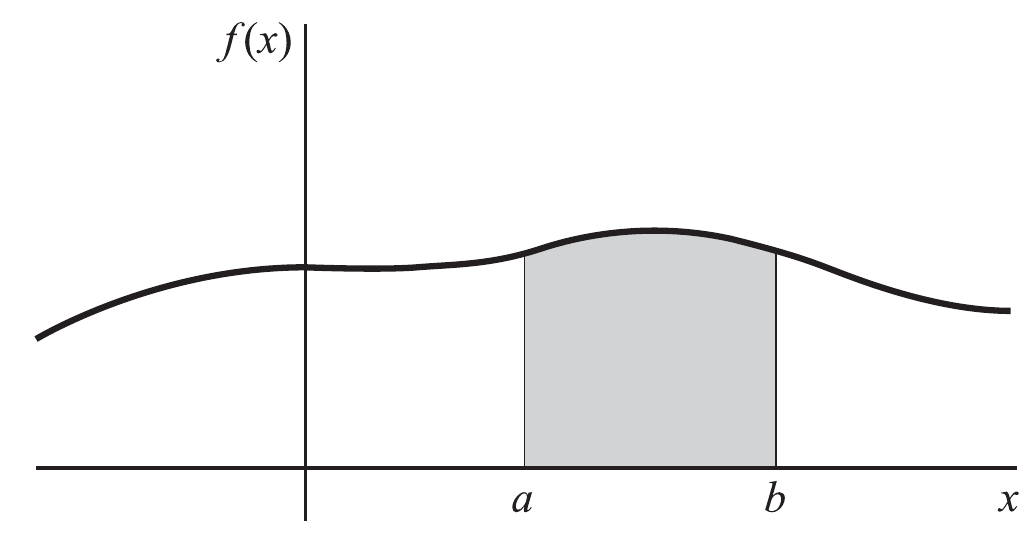
\includegraphics[height=5cm,keepaspectratio=true]{./pe/pands0202.png}
	% pands0202.png: 0x0 pixel, 300dpi, 0.00x0.00 cm, bb=
\end{figure}




  ...y el área bajo dicha curva es igual a $1.$
  \begin{figure}
	\centering
	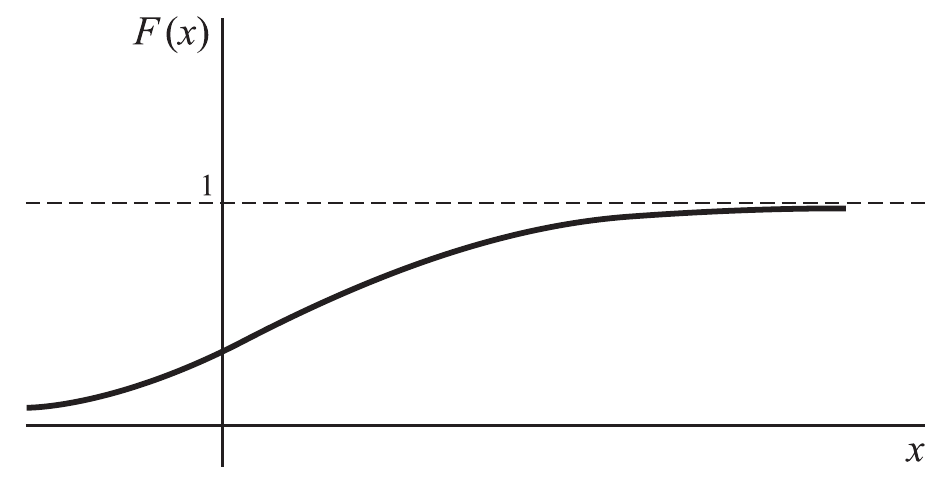
\includegraphics[height=5cm,keepaspectratio=true]{./pe/pands0203.png}
	% pands0203.png: 0x0 pixel, 300dpi, 0.00x0.00 cm, bb=
\end{figure}




\subsubsection{Distribución conjunta de probabilidad}


	Las ideas anteriores se generalizan fácilmente a dos o más variables.


{Caso discreto}
	Si $X$ y $Y$ son ambas variables aleatorias discretas, definimos la \emph{función de probabilidad conjunta} de $X$ y $Y$ por
	\begin{align}
	\label{eq:2.7.7}
		P(X=x, Y=y)=f(x,y)
	\end{align}
 donde
\begin{enumerate}
	\item $f(x,y)\geq 0;$
	\item $\sum_{k}\sum_{y}f(x,y)=1.$
\end{enumerate}




	Supongamos que $X$ sólo toma uno de los $m$ valores $x_{1},...,x_{m},$ mientras que $Y$ tomas sólo toma uno de los $n$ valores $y_{1},...,y_{n}.$

	Entonces la probabilidad del evento $X=x_{j}, Y=y_{k}$ está dada por
	\begin{align}
	\label{eq:2.7.8}
		P(X=x_{j}, Y=y_{k})=f(x_{j},y_{k})
	\end{align}



	Una función de probabilidad conjunta para $X$ y $Y$ puede ser representada por una \emph{tabla de probabilidad conjunta} como la siguiente:
	\begin{figure}
	\centering
		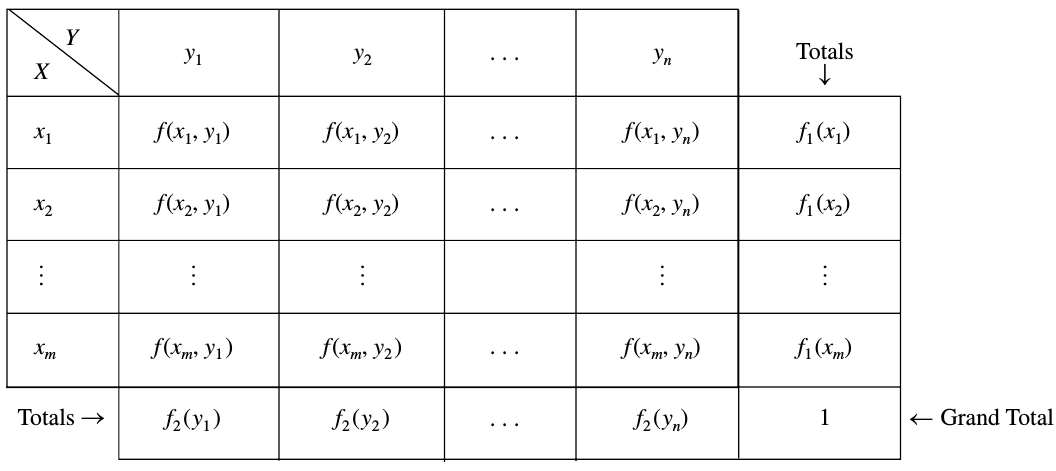
\includegraphics[height=5cm,keepaspectratio=true]{./pe/tab0203.png}
		% tab0203.png: 0x0 pixel, 300dpi, 0.00x0.00 cm, bb=
		\label{tab:2.7.1}
	\end{figure}



	La probabilidad de $X=x_{j}$ se obtiene de la siguiente manera
	\begin{align}
	\label{eq:2.7.9}
		P(X=x_{j})=f_{X}(x_{j})=\sum_{k=1}^{n}f(x_{j},y_{k}).
	\end{align}



	De manera similar, la probabilidad de $Y=y_{k}$ se obtiene de la siguiente manera
	\begin{align}
	\label{eq:2.7.10}
		P(Y=y_{k})=f_{Y}(y_{k})=\sum_{j=1}^{m}f(x_{j},y_{k}).
	\end{align}


 
 	Nos referiremos a $f_{X}(x)$ y $f_{Y}(y)$ como \emph{funciones de probabilidad marginal} de $X$ y $Y$ respectivamente.
 

	Observe que
	\begin{align}
	\label{eq:2.7.11}
		\sum_{j=1}^{m}f_{X}(x_{j})=1,
		\sum_{k=1}^{n}f_{Y}(y_{k})=1,
	\end{align}
	lo cual se puede reescribir como
	\begin{align}
		\label{eq:2.7.12}
		\sum_{j=1}^{m}\sum_{k=1}^{n}f(x_{j},y_{k})=1.
	\end{align}



	La \emph{función de distribución conjunta } está definida por
	\begin{align}
	\label{eq:2.7.13}
		F(x,y)=P(X\leq x, Y\leq y)
		=\sum_{u\leq x}\sum_{v\leq y}f(u,v)
	\end{align}



{Caso continuo}
	El caso en el que ambas variables son continuas es obtenido de manera análoga reemplazando las sumas por integrales.


	La \emph{función de probabilidad conjunta} (o de manera más común \emph{función de densidad conjunta}) de $X$y $Y$ está definida por
	\begin{enumerate}
		\item $f(x,y)\geq 0;$
		\item $\displaystyle \int_{-\infty}^{\infty}\int_{-\infty}^{\infty}
		f(x,y) dxdy=1.$
	\end{enumerate}



	Gráficamente $z=f(x,y)$ representa una \emph{superficie de probabilidad}
\begin{figure}
	\centering
		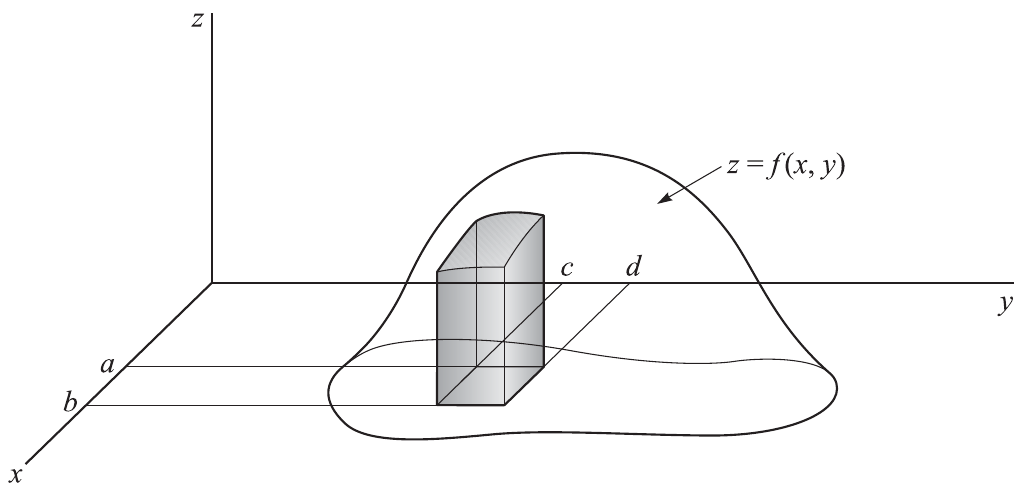
\includegraphics[height=3cm,keepaspectratio=true]{./pe/pands0204.png}
		% pands0204.png: 0x0 pixel, 300dpi, 0.00x0.00 cm, bb=
		\label{fig:2.7.1}
	\end{figure}
tal que el volumen bajo la superficie es igual a $1.$


	\begin{align}
		\label{eq:2.7.14}
		P(a<X<b,c<Y<d)=\int_{a}^{b}\int_{c}^{d}f(x,y)dydx.
	\end{align}



	A cada evento $A$ corresponde una región $\mathcal{R}_{A}$ del plano $xy$ tal que
	\begin{align}
	  \label{eq:2.7.15}
		P(A)=\iint_{\mathcal{R}_{A}}f(x,y)dxdy.
	\end{align}



	La \emph{función de distribución conjunta} de $X$ y $Y$ en este caso está definida por
	\begin{align}
		\label{eq:2.7.16}
	F(x,y)=P(X\leq x, Y\leq y)=
	\int_{-\infty}^{x} \int_{-\infty}^{y} f(u,v)dvdu.
	\end{align}



	Se sigue que
	\begin{align}
	 \dfrac{\partial^{2}F}{\partial x \partial y}=
	 f(x,y)  \label{eq:2.7.17} \\
	  	 P(X\leq x)=F_{X}(x)=\int_{-\infty}^{x}\int_{-\infty}^{\infty} f(u,v)dvdu \label{eq:2.7.18} \\
	 	 P(Y\leq y)=F_{Y}(y)=\int_{-\infty}^{\infty}\int_{-\infty}^{y} f(u,v)dvdu \label{eq:2.7.19}
	\end{align}



 Diremos que $F_{X}(x),F_{Y}(y)$ son las \emph{funciones de distribución marginal,} o simplemente \emph{funciones distribuciones,} de $X$ y $Y$, respectivamente.


 Las derivadas de \eqref{eq:2.7.18} y \eqref{eq:2.7.19} con respecto a $x$ y $y$ son llamadas \emph{funciones de densidad marginal}, o simplemente las \emph{funciones de densidad,} de $X$ y $Y$ están dados por
 \begin{align}
 \label{eq:2.7.20}
 \displaystyle
  f_{X}(x)=\int_{-\infty}^{\infty}f(x,v)dv, \;
  f_{Y}(y)=\int_{-\infty}^{\infty}f(u,y)du.
 \end{align}



 \subsubsection{Variables Aleatorias Independientes}

 Supongamos que $X$ y $Y$ son variables aleatorias discretas.  Si los eventos $X=x$ y $Y=y$ son eventos independientes para todo $x,y,$  entonces diremos que $X,Y$ son v.a's independientes.


 En tal caso,
 \begin{align}
  \label{eq:2.7.21}
  P(X=x,Y=y)=P(X=x)P(Y=y),
 \end{align}
o de manera equivalente
\begin{align}
 f(x,y)=f_{X}(x)f_{Y}(y).
\end{align}



 De manera inversa, si para todo $x,y$ la función de probabilidad conjunta $f(x,y)$ pueden ser expresada como el producto de funciones de probabilidad marginal $f_{X}(x)f_{Y}(y),$ entonces $X,Y$ son independientes.


 Si no pueden expresarse de dicha manera, entonces $X,Y$ son dependientes.


 Si $X,Y$ son v.a's continuas, diremos que son \emph{independientes} si los eventos $X\leq x$ y $Y\leq y$ son independientes para todo $x,y.$

 En tal caso, escribiremos
 \begin{align}
  \label{eq:2.7.22}
  P(X\leq x, Y \leq y)=P(X\leq x)P(Y\leq y)
 \end{align}
 o de manera equivalente
 \begin{align}
  F(x,y)=F_{X}(x)F_{Y}(y)
 \end{align}
 donde $F_{X}(x)$ y $F_{Y}(y)$ son las funciones de distribución marginal de $X,Y$ respectivamente.



 De manera inversa, si para todo $x,y$ la función de probabilidad conjunta $f(x,y)$ pueden ser expresada como el producto de funciones de probabilidad marginal $F_{X}(x)F_{Y}(y),$ entonces $X,Y$ son independientes.
 

 Si no pueden expresarse de dicha manera, entonces $X,Y$ son dependientes.


 Para v.a's independientes continuas, también es cierto que la función de densidad conjunta $f(x,y)$ es el producto de funciones $f_{X}(x)f_{Y}(y)$ y estas son las funciones de densidad marginal de $X,Y$ respectivamente.



 \begin{ejemplo}
  \label{exmp:2.7.6}
  La función de probabilidad conjunta de dos variables discretas $X,Y$ está dada por
  \begin{align}
   f(x,y)=
   \begin{cases}
    c(2x+y) & 0\leq x \leq 2, \; 0 \leq y \leq 3 \\
    0 & \texttt{en otro caso}.
   \end{cases}
  \end{align}
  \begin{enumerate}
   \item Encuentre el valor de la constante $c;$
   \item encuentre $P(X=2,Y=1);$
   \item encuentre $P(X\geq 1, Y\leq 2).$
  \end{enumerate}

 \end{ejemplo}



 \begin{figure}
 \centering
	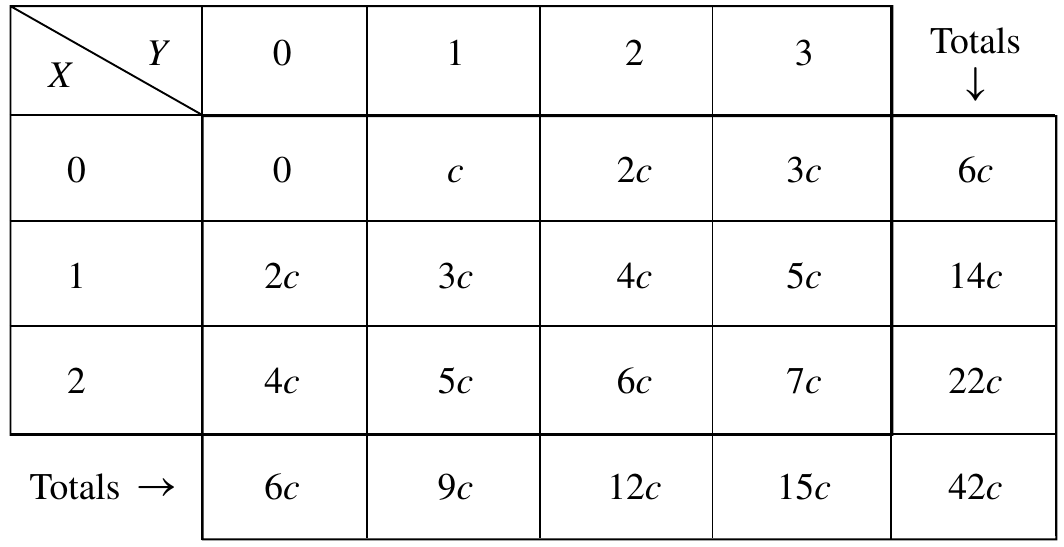
\includegraphics[width=10cm,keepaspectratio=true]{./pe/tab0206.png}
	% tab0206.png: 0x0 pixel, 300dpi, 0.00x0.00 cm, bb=
	\label{tab:2.7.2}
\end{figure}



\begin{ejemplo}
  \label{exmp:2.7.7}
  Encuentre las funciones de probabilidad marginal para $X$ y $Y$ en el problema resuelto \ref{exmp:2.7.6}.
\end{ejemplo}



\begin{ejemplo}
  \label{exmp:2.7.8}
  Muestre que las variables aleatorias del problema resuelto \ref{exmp:2.7.6} son dependientes.
\end{ejemplo}



\begin{ejemplo}
  \label{exmp:2.7.9}
  La función de densidad conjunta de dos variables aleatorias continuas $X$ y $Y$ es
  \begin{align}
   f(x,y)=
   \begin{cases}
    cxy & 0<x<4, \; 1<y<5\\
    0 & \texttt{en otro caso}.
   \end{cases}
  \end{align}

 \end{ejemplo}
\begin{enumerate}
 \item Encuentre el valor de $c$;
 \item encuentre $P(1<X<2,2<Y<3)$;
 \item encuentre $P(X\geq 3, Y\leq 2)$.
\end{enumerate}



\begin{ejemplo}
  \label{exmp:2.7.10}
  Encuentre las funciones de probabilidad marginal de las v.a's $X,Y$ del problema resuelto \ref{exmp:2.7.9}.
\end{ejemplo}



\begin{ejemplo}
  \label{exmp:2.7.11}
  Encuentre la función de distribución conjunta para las v.a's del problema resuelto \ref{exmp:2.7.9}.
\end{ejemplo}



 \begin{center}
 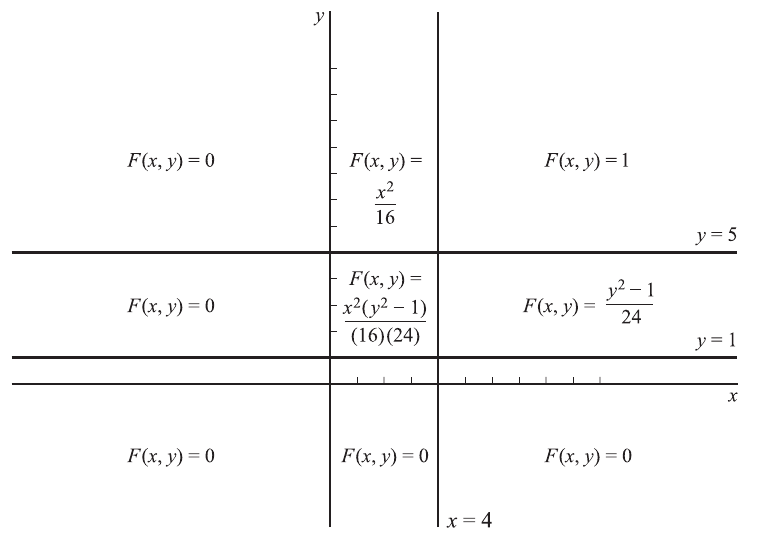
\includegraphics[width=10cm,keepaspectratio=true]{./pe/pands0209.png}
 % pands0209.png: 0x0 pixel, 300dpi, 0.00x0.00 cm, bb=
\end{center}




\begin{ejemplo}
  \label{exmp:2.7.12}
  En el problema resuelto \ref{exmp:2.7.9}, encuentre $P(X+Y<3)$.
\end{ejemplo}



 \begin{center}
 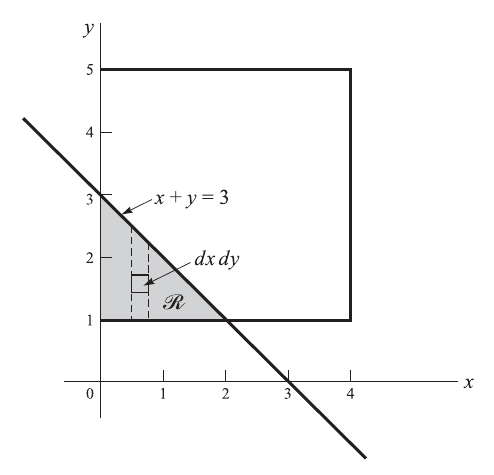
\includegraphics[height=8cm,keepaspectratio=true]{./pe/pands0210.png}
 % pands0210.png: 0x0 pixel, 300dpi, 0.00x0.00 cm, bb=
\end{center}



 \subsubsection{Distribución Condicional}

 Nosotros ya sabemos que si $P(A)>0,$
 \begin{align}
  \label{eq:2.7.23}
  P(B|A)=\dfrac{P(A\cap B)}{P(A)}.
 \end{align}



 Si $X,Y$ son v.a's discretas y tenemos los eventos $A=\set{X=x}, \; B=\set{Y=y},$ entonces \eqref{eq:2.7.23} se convierte
 \begin{align}
  \label{eq:2.7.24}
  P(Y=y|X=x)=
  \begin{cases}
   \dfrac{f(x,y)}{f_{X}(x)} & 0 < f_{X}(x)  \\
   0 & \texttt{en otro caso}
  \end{cases}
 \end{align}
 $f(x,y)=P(X=x,Y=y)$ es la función de probabilidad conjunta, mientras que $f_{X}(x)$ es la función de probabilidad marginal para $X.$


 Definimos la \emph{función de probabilidad condicional de $Y$ dado $X$} como
 \begin{align}
  \label{eq:2.7.25}
  f(y|x)=
  \begin{cases}
   \dfrac{f(x,y)}{f_{X}(x)} & 0 < f_{X}(x)  \\
   0 & \texttt{en otro caso}
  \end{cases}
 \end{align}



 De manera similar, definimos la \emph{función de probabilidad condicional de $X$ dado $Y$} como
 \begin{align}
  \label{eq:2.7.26}
  f(x|y)=
  \begin{cases}
   \dfrac{f(x,y)}{f_{Y}(y)} & 0 < f_{Y}(y)  \\
   0 & \texttt{en otro caso}
  \end{cases}
 \end{align}


 Estas ideas son fácilmente extensibles al caso donde $X,Y$ son v.a's continuas.


 Por ejemplo, la \emph{función de densidad condicional de $Y$ dado $X$} es
 \begin{align}
  \label{eq:2.7.27}
  f(y|x)=
    \begin{cases}
   \dfrac{f(x,y)}{f_{X}(x)} & 0 < f_{X}(x)  \\
   0 & \texttt{en otro caso}
  \end{cases}
 \end{align}
 donde $f(x,y)$ es la función de densidad conjunta de $X$ y $Y$ y $f_{X}(x)$ es la función de densidad marginal de $X.$


 Usando \eqref{eq:2.7.27} podemos por ejemplo encontrar que la probabilidad que $Y$  se encuentre entre $c$ y $d$ dado que $X=x$ es
 \begin{align}
  \label{eq:2.7.28}P(c<Y<d|X=x)=
  \int_{c}^{d}f(y|x)dy.
 \end{align}




 \begin{ejemplo}
  \label{exmp:2.7.13}
  Para la distribución del problema resuelto \ref{exmp:2.7.6}, encuentre
  \begin{enumerate}
   \item $f(y|2)$; y
   \item $P(Y=1|X=2)$
  \end{enumerate}

 \end{ejemplo}



\begin{ejemplo}
 \label{exmp:2.7.14}
  Si $X$ y $Y$ tienen función de densidad conjunta
 \begin{align}
  f(x,y)=
  \begin{cases}
   \frac{3}{4}+xy & 0<x<1, \; 0<y<1 \\
   0 & \texttt{en otro caso},
  \end{cases}
 \end{align}
encuentre
\begin{enumerate}
 \item $f(y|x)$; 
 \item $P(Y>\frac{1}{2}| X = \frac{1}{2} )$.
\end{enumerate}

\end{ejemplo}



 \begin{ejemplo}
  \label{exmp:2.7.15}
  La función de densidad conjunta de las variables aleatorias $X$ y $Y$ está dada por
  \begin{align}
   f(x,y)=
   \begin{cases}
    8xy & 0\leq x \leq 1, 0\leq y \leq x \\
    0 & \texttt{en otro caso}.
   \end{cases}
  \end{align}
Encuentre
\begin{enumerate}
 \item la densidad marginal de $X$; 
 \item la densidad marginal de $Y$; 
 \item la densidad condicional de $X$; 
 \item la densidad condicional de $Y$.
\end{enumerate}

 \end{ejemplo}



 \begin{center}
 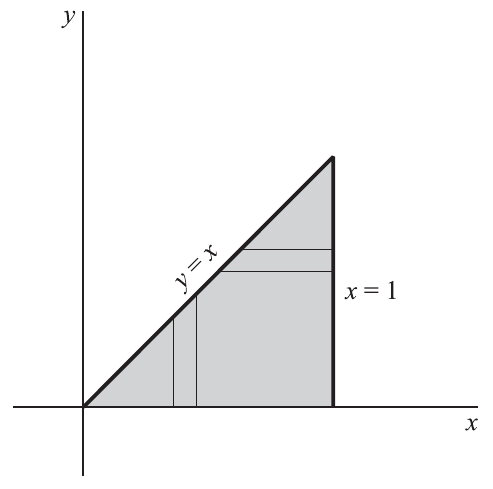
\includegraphics[height=7cm,keepaspectratio=true]{./pe/pands0217.png}
 % pands0217.png: 0x0 pixel, 300dpi, 0.00x0.00 cm, bb=
\end{center}



 \begin{ejemplo}
  \label{exmp:2.7.16}
  Determine si las v.a's del problema resuelto \ref{exmp:2.7.15} son independientes.
 \end{ejemplo}



% ==============================================================================
% SECCIÓN 04.01: FUNCIÓN DE DENSIDAD DE PROBABILIDAD (PDF) Y SOPORTE CONTINUO
% ==============================================================================

\subsection*{Enunciados de los problemas --- Sección 04.01}

\subsubsection*{Nivel Fundamental}

\begin{problema}
	\label{prob:4.1.1}
	Considere la función $f(x) = c \cdot e^{-x}$ para $x \ge 0$ y $f(x) = 0$ para $x < 0$, donde $c$ es una constante positiva.
	\begin{enumerate}
		\item Determine el valor de $c$ tal que $f(x)$ sea una función de densidad de probabilidad (PDF) válida.
		\item Calcule la probabilidad $P(1 \le X \le 3)$ integrando la PDF en el intervalo.
		\item Calcule la función de distribución acumulada (CDF) $F(x)$ para todo $x \in \mathbb{R}$.
	\end{enumerate}
\end{problema}

\begin{problema}
	\label{prob:4.1.2}
	Una variable aleatoria continua $X$ tiene PDF dada por:
	$$f(x) = \begin{cases} c \cdot (4x - 2x^{2}) & \text{si } 0 \le x \le 2 \\ 0 & \text{en otro caso} \end{cases}$$
	\begin{enumerate}
		\item Encuentre la constante de normalización $c$ tal que $\int_{-\infty}^{\infty} f(x)\,dx = 1$.
		\item Calcule $P(X \ge 1)$ y $P(0.5 \le X \le 1.5)$.
	\end{enumerate}
\end{problema}

\begin{problema}
	\label{prob:4.1.3}
	Sea $X$ una variable aleatoria con PDF triangular:
	$$f(x) = \begin{cases} x & \text{si } 0 \le x \le 1 \\ 2 - x & \text{si } 1 < x \le 2 \\ 0 & \text{en otro caso} \end{cases}$$
	\begin{enumerate}
		\item Verifique que $\int_{-\infty}^{\infty} f(x)\,dx = 1$.
		\item Calcule la moda (el valor donde $f$ es máxima) y la mediana (el valor $m$ tal que $P(X \le m) = 0.5$).
	\end{enumerate}
\end{problema}

\subsubsection*{Nivel Operativo}

\begin{problema}
	\label{prob:4.1.4}
	Sea $X$ una variable aleatoria continua con CDF $F(x) = 1 - e^{-x^{2}/2}$ para $x \ge 0$ y $F(x) = 0$ para $x < 0$ (distribución de Rayleigh).
	\begin{enumerate}
		\item Derive la PDF $f(x)$ aplicando $f(x) = F'(x)$.
		\item Verifique que $\int_{0}^{\infty} f(x)\,dx = 1$ usando la sustitución $u = x^{2}/2$.
		\item Calcule la mediana $m$ tal que $F(m) = 0.5$.
	\end{enumerate}
\end{problema}

\begin{problema}
	\label{prob:4.1.5}
	Considere la PDF definida por:
	$$f(x) = \begin{cases} \dfrac{3}{8}(2 - x^{2}) & \text{si } -1 \le x \le 1 \\ 0 & \text{en otro caso} \end{cases}$$
	\begin{enumerate}
		\item Verifique que $f$ integra a $1$.
		\item Calcule $P(-0.5 \le X \le 0.5)$ y $P(X \ge 0)$.
		\item Halle la CDF $F(x)$ para $x \in [-1, 1]$ y grafique cualitativamente su forma.
	\end{enumerate}
\end{problema}

\begin{problema}
	\label{prob:4.1.6}
	En un sistema de comunicaciones, el tiempo de espera $X$ (en milisegundos) hasta la recepción de un paquete tiene PDF exponencial con parámetro $\lambda = 0.5$ ms$^{-1}$:
	$$f(x) = 0.5 \cdot e^{-0.5 x}, \quad x \ge 0$$
	\begin{enumerate}
		\item Calcule la probabilidad $P(X \le 1)$ de que el tiempo de espera sea menor a 1 ms.
		\item Calcule $P(2 \le X \le 5)$ mediante integración de la PDF.
		\item Halle la mediana $m$ tal que $P(X \le m) = 0.5$.
	\end{enumerate}
\end{problema}

\subsubsection*{Nivel Analítico}

\begin{problema}
	\label{prob:4.1.7}
	Sea $X$ una variable aleatoria continua con PDF $f(x)$. Demuestre formalmente que la esperanza matemática puede calcularse como:
	$$\E[X] = \int_{-\infty}^{\infty} x \cdot f(x)\,dx$$
	partiendo de la definición $\E[X] = \int x\,dF(x)$ y usando integración por partes bajo condiciones técnicas de regularidad.
\end{problema}

\begin{problema}
	\label{prob:4.1.8}
	Para una variable aleatoria continua $X$ con PDF $f(x)$ y una función $g: \mathbb{R} \to \mathbb{R}$, demuestre el \emph{Teorema LOTUS Continuo} (Law of the Unconscious Statistician):
	$$\E[g(X)] = \int_{-\infty}^{\infty} g(x) \cdot f(x)\,dx$$
	\begin{enumerate}
		\item Demuestre el caso particular $g(X) = X^{2}$.
		\item Derive la fórmula de la varianza $\Var(X) = \E[X^{2}] - (\E[X])^{2}$ usando LOTUS con $g(x) = (x - \mu)^{2}$.
	\end{enumerate}
\end{problema}

\subsubsection*{Nivel Desafiante}

\begin{problema}
	\label{prob:4.1.9}
	Considere una distribución mixta continua-discreta donde $X$ toma el valor $0$ con probabilidad $1/3$ y, condicionalmente a $X > 0$, sigue una distribución exponencial con parámetro $\lambda = 2$:
	$$f(x) = \begin{cases} 1/3 & \text{si } x = 0 \\ (2/3) \cdot 2 e^{-2x} & \text{si } x > 0 \\ 0 & \text{en otro caso} \end{cases}$$
	\begin{enumerate}
		\item Verifique que $f$ es una PDF válida (masa puntual en $0$ + densidad exponencial).
		\item Calcule la CDF $F(x)$ para todo $x \in \mathbb{R}$, identificando el salto en $x = 0$.
		\item Calcule $\E[X]$ y $\Var(X)$ usando la ley total de esperanza.
	\end{enumerate}
\end{problema}

\begin{problema}
	\label{prob:4.1.10}
	En teoría de señales, la convolución de dos densidades $f$ y $g$ produce la densidad de la suma $Z = X + Y$ de dos variables aleatorias independientes:
	$$h(z) = (f * g)(z) = \int_{-\infty}^{\infty} f(x) \cdot g(z - x)\,dx$$
	\begin{enumerate}
		\item Demuestre que si $X \sim N(0, 1)$ y $Y \sim N(0, 1)$ son independientes, entonces $Z = X + Y$ tiene PDF $N(0, 2)$, es decir, $\Var(Z) = \Var(X) + \Var(Y)$.
		\item Generalice: si $X_{1}, \dots, X_{n}$ son i.i.d. $N(0, \sigma^{2})$, entonces $\sum_{i=1}^{n} X_{i} \sim N(0, n\sigma^{2})$.
		\item Interprete este resultado en el contexto de filtrado de ruido gaussiano en telecomunicaciones.
	\end{enumerate}
\end{problema}

\subsection*{Sugerencias de los problemas --- Sección 04.01}

\begin{sugerencia}
	\label{sug:4.1.1}
	Para el Problema \ref{prob:4.1.1}, integre $\int_{0}^{\infty} c \cdot e^{-x}\,dx = c = 1$, así que $c = 1$. Para $P(1 \le X \le 3) = e^{-1} - e^{-3} \approx 0.318$. La CDF es $F(x) = 1 - e^{-x}$ para $x \ge 0$.
\end{sugerencia}

\begin{sugerencia}
	\label{sug:4.1.2}
	Para el Problema \ref{prob:4.1.2}, integre $\int_{0}^{2} c(4x - 2x^{2})\,dx = c \cdot [2x^{2} - 2x^{3}/3]_{0}^{2} = c(8 - 16/3) = 8c/3 = 1$, dando $c = 3/8$. Para $P(X \ge 1)$, integre desde $1$ hasta $2$.
\end{sugerencia}

\begin{sugerencia}
	\label{sug:4.1.3}
	Para el Problema \ref{prob:4.1.3}, la moda está en $x = 1$ (donde la PDF alcanza el máximo de $1$). La integral $\int_{0}^{1} x\,dx = 1/2$ y $\int_{1}^{2} (2-x)\,dx = 1/2$, sumando a $1$. La mediana $m$ satisface $\int_{0}^{m} x\,dx = 0.5$ si $m \le 1$, dando $m = 1$.
\end{sugerencia}

\begin{sugerencia}
	\label{sug:4.1.4}
	Para el Problema \ref{prob:4.1.4}, $f(x) = F'(x) = x e^{-x^{2}/2}$ para $x \ge 0$. Con la sustitución $u = x^{2}/2$, $du = x\,dx$: $\int_{0}^{\infty} x e^{-x^{2}/2}\,dx = \int_{0}^{\infty} e^{-u}\,du = 1$. La mediana satisface $1 - e^{-m^{2}/2} = 0.5$, dando $m = \sqrt{2 \ln 2} \approx 1.177$.
\end{sugerencia}

\begin{sugerencia}
	\label{sug:4.1.5}
	Para el Problema \ref{prob:4.1.5}, $\int_{-1}^{1} (3/8)(2 - x^{2})\,dx = (3/8)[2x - x^{3}/3]_{-1}^{1} = (3/8)(4 - 2/3) = (3/8)(10/3) = 10/8 \ne 1$. Verifique: $\int_{-1}^{1} (2 - x^{2})\,dx = [2x - x^{3}/3]_{-1}^{1} = (2 - 1/3) - (-2 + 1/3) = 4 - 2/3 = 10/3$. Por lo tanto $c = 3/10$ para que la integral sea $1$.
\end{sugerencia}

\begin{sugerencia}
	\label{sug:4.1.6}
	Para el Problema \ref{prob:4.1.6}, la CDF exponencial es $F(x) = 1 - e^{-0.5 x}$. Entonces $P(X \le 1) = 1 - e^{-0.5} \approx 0.393$. $P(2 \le X \le 5) = e^{-1} - e^{-2.5} \approx 0.3679 - 0.0821 = 0.286$. La mediana es $m = -\ln(0.5)/0.5 = 2 \ln 2 \approx 1.386$ ms.
\end{sugerencia}

\begin{sugerencia}
	\label{sug:4.1.7}
	Para el Problema \ref{prob:4.1.7}, use la representación $F(x) = \int_{-\infty}^{x} f(t)\,dt$ y la integración por partes $\int x\,dF(x) = xF(x) - \int F(x)\,dx$. Asumiendo $\lim_{x \to \pm\infty} xF(x) = 0$ (condición técnica de colas ligeras), sustituya la CDF y simplifique para obtener $\E[X] = \int x f(x)\,dx$.
\end{sugerencia}

\begin{sugerencia}
	\label{sug:4.1.8}
	Para el Problema \ref{prob:4.1.8}, use que para variables aleatorias continuas, $\E[g(X)] = \int g(x) f(x)\,dx$ donde $f$ es la densidad. El caso $g(X) = X^{2}$ se obtiene directamente. Para la varianza, $g(X) = (X - \mu)^{2}$ con $\mu = \E[X]$, dando $\E[(X-\mu)^{2}] = \E[X^{2}] - 2\mu\E[X] + \mu^{2} = \E[X^{2}] - \mu^{2}$.
\end{sugerencia}

\begin{sugerencia}
	\label{sug:4.1.9}
	Para el Problema \ref{prob:4.1.9}, la masa en $0$ es $1/3$ y la densidad exponencial reescalada $(2/3) \cdot 2 e^{-2x}$ integra a $\int_{0}^{\infty} (4/3) e^{-2x}\,dx = (4/3) \cdot (1/2) = 2/3$. Sumando: $1/3 + 2/3 = 1$. La CDF tiene un salto de $1/3$ en $x = 0$ y luego crece según la exponencial reescalada.
\end{sugerencia}

\begin{sugerencia}
	\label{sug:4.1.10}
	Para el Problema \ref{prob:4.1.10}, la convolución de dos gaussianas es gaussiana con varianzas sumadas. Demuestre usando la forma explícita de la PDF: $h(z) = \int (2\pi)^{-1} \exp(-x^{2}/2) \cdot \exp(-(z-x)^{2}/2)\,dx$. Complete el cuadrado en el exponente y use la integral gaussiana.
\end{sugerencia}

\subsection*{Soluciones de los problemas --- Sección 04.01}

\begin{solucion}
	\label{sol:4.1.1}
	Para el Problema \ref{prob:4.1.1}:
	\begin{enumerate}
		\item La condición de normalización requiere:
		\begin{align*}
			\int_{-\infty}^{\infty} f(x)\,dx = \int_{0}^{\infty} c \cdot e^{-x}\,dx = c \cdot [-e^{-x}]_{0}^{\infty} = c \cdot 1 = c = 1.
		\end{align*}
		Por lo tanto, $c = 1$.
		\item La probabilidad es:
		\begin{align*}
			P(1 \le X \le 3) = \int_{1}^{3} e^{-x}\,dx = [-e^{-x}]_{1}^{3} = e^{-1} - e^{-3} \approx 0.3679 - 0.0498 = 0.3181.
		\end{align*}
		\item La CDF se obtiene integrando desde $-\infty$ hasta $x$:
		\begin{align*}
			F(x) &= \int_{-\infty}^{x} f(t)\,dt = \begin{cases} 0 & \text{si } x < 0 \\ \int_{0}^{x} e^{-t}\,dt = 1 - e^{-x} & \text{si } x \ge 0 \end{cases}
		\end{align*}
		Esta es la CDF de la distribución exponencial con parámetro $\lambda = 1$.
	\end{enumerate}
\end{solucion}

\begin{solucion}
	\label{sol:4.1.2}
	Para el Problema \ref{prob:4.1.2}:
	\begin{enumerate}
		\item La condición de normalización es:
		\begin{align*}
			1 = \int_{0}^{2} c(4x - 2x^{2})\,dx = c \left[ 2x^{2} - \dfrac{2x^{3}}{3} \right]_{0}^{2} = c \left( 8 - \dfrac{16}{3} \right) = \dfrac{8c}{3}.
		\end{align*}
		Por lo tanto, $c = 3/8$.
		\item Para $P(X \ge 1)$:
		\begin{align*}
			P(X \ge 1) = \int_{1}^{2} \dfrac{3}{8}(4x - 2x^{2})\,dx = \dfrac{3}{8} \left[ 2x^{2} - \dfrac{2x^{3}}{3} \right]_{1}^{2} = \dfrac{3}{8} \cdot \left[ \left( 8 - \dfrac{16}{3} \right) - \left( 2 - \dfrac{2}{3} \right) \right] = \dfrac{3}{8} \cdot \dfrac{4}{3} = \dfrac{1}{2}.
		\end{align*}
		Para $P(0.5 \le X \le 1.5)$:
		\begin{align*}
			P(0.5 \le X \le 1.5) = \dfrac{3}{8} \left[ 2x^{2} - \dfrac{2x^{3}}{3} \right]_{0.5}^{1.5} = \dfrac{3}{8} \left[ \left( \dfrac{9}{2} - \dfrac{9}{4} \right) - \left( \dfrac{1}{2} - \dfrac{1}{12} \right) \right] = \dfrac{3}{8} \cdot \dfrac{5}{3} = \dfrac{5}{8}.
		\end{align*}
	\end{enumerate}
\end{solucion}

\begin{solucion}
	\label{sol:4.1.3}
	Para el Problema \ref{prob:4.1.3}:
	\begin{enumerate}
		\item Verificamos la normalización:
		\begin{align*}
			\int_{0}^{1} x\,dx + \int_{1}^{2} (2 - x)\,dx = \dfrac{1}{2} + \left[ 2x - \dfrac{x^{2}}{2} \right]_{1}^{2} = \dfrac{1}{2} + \left( 4 - 2 \right) - \left( 2 - \dfrac{1}{2} \right) = \dfrac{1}{2} + \dfrac{1}{2} = 1. \quad \checkmark
		\end{align*}
		\item La moda está en $x = 1$ (donde la PDF alcanza el máximo $f(1) = 1$). Para la mediana $m$: si $m \le 1$, $\int_{0}^{m} x\,dx = m^{2}/2 = 0.5$, dando $m = 1$. Como $m = 1$ también marca la frontera entre las dos ramas, es exactamente la mediana. Por la simetría de la triangular alrededor de $x = 1$, concluimos que \emph{moda $=$ mediana $= 1$}.
	\end{enumerate}
\end{solucion}

\begin{solucion}
	\label{sol:4.1.4}
	Para el Problema \ref{prob:4.1.4}:
	\begin{enumerate}
		\item Derivando la CDF:
		\begin{align*}
			f(x) = F'(x) = \dfrac{d}{dx}\left( 1 - e^{-x^{2}/2} \right) = x e^{-x^{2}/2}, \quad x \ge 0.
		\end{align*}
		\item Verificamos la normalización con la sustitución $u = x^{2}/2$, $du = x\,dx$:
		\begin{align*}
			\int_{0}^{\infty} x e^{-x^{2}/2}\,dx = \int_{0}^{\infty} e^{-u}\,du = [-e^{-u}]_{0}^{\infty} = 1 - 0 = 1. \quad \blacksquare
		\end{align*}
		\item La mediana satisface $1 - e^{-m^{2}/2} = 0.5$, es decir, $e^{-m^{2}/2} = 0.5$. Tomando logaritmo: $-m^{2}/2 = -\ln 2$, así $m = \sqrt{2 \ln 2} \approx 1.1774$.
	\end{enumerate}
\end{solucion}

\begin{solucion}
	\label{sol:4.1.5}
	Para el Problema \ref{prob:4.1.5}:
	\begin{enumerate}
		\item Verificamos la normalización:
		\begin{align*}
			\int_{-1}^{1} c(2 - x^{2})\,dx = c \left[ 2x - \dfrac{x^{3}}{3} \right]_{-1}^{1} = c \left[ \left( 2 - \dfrac{1}{3} \right) - \left( -2 + \dfrac{1}{3} \right) \right] = c \cdot \dfrac{10}{3}.
		\end{align*}
		Para que la integral sea $1$: $c = 3/10$. La PDF correcta es $f(x) = \dfrac{3}{10}(2 - x^{2})$ para $x \in [-1, 1]$.
		\item Para $P(-0.5 \le X \le 0.5)$:
		\begin{align*}
			P(-0.5 \le X \le 0.5) = \int_{-0.5}^{0.5} \dfrac{3}{10}(2 - x^{2})\,dx = \dfrac{3}{10}\left[ 2x - \dfrac{x^{3}}{3} \right]_{-0.5}^{0.5} = \dfrac{3}{10} \cdot 2 = 0.6.
		\end{align*}
		Para $P(X \ge 0)$ (por simetría de la PDF): $P(X \ge 0) = 0.5$.
		\item La CDF es:
		\begin{align*}
			F(x) = \int_{-1}^{x} \dfrac{3}{10}(2 - t^{2})\,dt = \dfrac{3}{10}\left( 2x + 2 - \dfrac{x^{3}}{3} - \dfrac{1}{3} \right) = \dfrac{3}{10}\left( \dfrac{6x - x^{3} + 5}{3} \right) = \dfrac{6x - x^{3} + 5}{10}.
		\end{align*}
		Verificación: $F(-1) = (-6 + 1 + 5)/10 = 0$ ✓, $F(1) = (6 - 1 + 5)/10 = 1$ ✓.
	\end{enumerate}
\end{solucion}

\begin{solucion}
	\label{sol:4.1.6}
	Para el Problema \ref{prob:4.1.6}, la CDF exponencial con parámetro $\lambda = 0.5$ es $F(x) = 1 - e^{-0.5 x}$ para $x \ge 0$.
	\begin{enumerate}
		\item $P(X \le 1) = 1 - e^{-0.5 \cdot 1} = 1 - e^{-0.5} \approx 1 - 0.6065 = 0.3935$.
		\item $P(2 \le X \le 5) = F(5) - F(2) = (1 - e^{-2.5}) - (1 - e^{-1}) = e^{-1} - e^{-2.5} \approx 0.3679 - 0.0821 = 0.2858$.
		\item La mediana satisface $1 - e^{-0.5 m} = 0.5$, es decir, $e^{-0.5 m} = 0.5$. Tomando logaritmo: $m = -2 \ln(0.5) = 2 \ln 2 \approx 1.386$ ms.
	\end{enumerate}
\end{solucion}

\begin{solucion}
	\label{sol:4.1.7}
	Para el Problema \ref{prob:4.1.7}, partimos de la definición $\E[X] = \int_{-\infty}^{\infty} x\,dF(x)$. Usando integración por partes con $u = x$ y $dv = dF(x)$:
	\begin{align*}
		\E[X] &= \int_{-\infty}^{\infty} x\,dF(x) = \left[ xF(x) \right]_{-\infty}^{\infty} - \int_{-\infty}^{\infty} F(x)\,dx.
	\end{align*}
	Asumiendo la condición técnica de colas ligeras $\lim_{x \to \pm\infty} xF(x) = 0$ (lo cual se cumple si $\int |x| f(x)\,dx < \infty$):
	\begin{align*}
		\E[X] &= - \int_{-\infty}^{\infty} F(x)\,dx.
	\end{align*}
	Sustituyendo $F(x) = \int_{-\infty}^{x} f(t)\,dt$:
	\begin{align*}
		\E[X] &= - \int_{-\infty}^{\infty} \int_{-\infty}^{x} f(t)\,dt\,dx = - \int_{-\infty}^{\infty} f(t) \left( \int_{t}^{\infty} dx \right) dt = - \int_{-\infty}^{\infty} f(t) \cdot (\infty - t)\,dt.
		\end{align*}
		Este enfoque no es el más limpio. Procedamos de manera más directa. Recordando que $dF(x) = f(x)\,dx$:
		\begin{align*}
			\E[X] = \int_{-\infty}^{\infty} x \cdot dF(x) = \int_{-\infty}^{\infty} x \cdot f(x)\,dx. \quad \blacksquare
		\end{align*}
		La sustitución directa $dF = f\,dx$ es la forma operacional del teorema, válida bajo la condición de integrabilidad absoluta $\int |x| f(x)\,dx < \infty$.
\end{solucion}

\begin{solucion}
	\label{sol:4.1.8}
	Para el Problema \ref{prob:4.1.8}:
	\begin{enumerate}
		\item Para $g(X) = X^{2}$, usamos que la PDF de $X^{2}$ se obtiene mediante la transformación. Sin embargo, la forma más directa es usar la definición operacional de LOTUS:
		\begin{align*}
			\E[X^{2}] = \int_{-\infty}^{\infty} x^{2} f(x)\,dx,
		\end{align*}
		que es simplemente la definición de esperanza con $g(x) = x^{2}$.
		\item Para la varianza con $g(X) = (X - \mu)^{2}$ donde $\mu = \E[X]$:
		\begin{align*}
			\Var(X) &= \E[(X - \mu)^{2}] = \int_{-\infty}^{\infty} (x - \mu)^{2} f(x)\,dx \\
			&= \int_{-\infty}^{\infty} (x^{2} - 2\mu x + \mu^{2}) f(x)\,dx \\
			&= \E[X^{2}] - 2\mu \E[X] + \mu^{2} \\
			&= \E[X^{2}] - 2\mu^{2} + \mu^{2} = \E[X^{2}] - (\E[X])^{2}. \quad \blacksquare
		\end{align*}
		donde usamos linealidad de la integral y la constancia de $\mu$ bajo la integral.
	\end{enumerate}
\end{solucion}

\begin{solucion}
	\label{sol:4.1.9}
	Para el Problema \ref{prob:4.1.9}:
	\begin{enumerate}
		\item La masa puntual en $x = 0$ es $1/3$, y la densidad exponencial reescalada $(2/3) \cdot 2 e^{-2x} = (4/3) e^{-2x}$ para $x > 0$ integra a:
		\begin{align*}
			\int_{0}^{\infty} \dfrac{4}{3} e^{-2x}\,dx = \dfrac{4}{3} \cdot \dfrac{1}{2} = \dfrac{2}{3}.
		\end{align*}
		Sumando: $1/3 + 2/3 = 1$. La PDF es válida.
		\item La CDF tiene un salto en $x = 0$ y luego crece continuamente:
		\begin{align*}
			F(x) = \begin{cases} 0 & \text{si } x < 0 \\ 1/3 & \text{si } x = 0 \\ 1/3 + \int_{0}^{x} \dfrac{4}{3} e^{-2t}\,dt = 1/3 + \dfrac{2}{3}(1 - e^{-2x}) = 1 - \dfrac{2}{3} e^{-2x} & \text{si } x > 0 \end{cases}
		\end{align*}
		El salto en $x = 0$ es $F(0) - F(0^{-}) = 1/3 - 0 = 1/3$, correspondiente a la masa puntual.
		\item Usando la ley total de esperanza $\E[X] = \E[\E[X \mid Z]]$ con $Z$ indicador de $X = 0$:
		\begin{align*}
			\E[X] = \Prob(X = 0) \cdot 0 + \Prob(X > 0) \cdot \E[X \mid X > 0].
		\end{align*}
		Condicionalmente a $X > 0$, $X$ sigue $\text{Exp}(2)$ con media $1/2$. Por lo tanto:
		\begin{align*}
			\E[X] = \dfrac{1}{3} \cdot 0 + \dfrac{2}{3} \cdot \dfrac{1}{2} = \dfrac{1}{3}.
		\end{align*}
		Para la varianza, $\Var(X) = \E[X^{2}] - (\E[X])^{2}$. Con $\E[X^{2} \mid X > 0] = 2/4 = 1/2$ (segundo momento de Exp(2)):
		\begin{align*}
			\E[X^{2}] = \dfrac{1}{3} \cdot 0 + \dfrac{2}{3} \cdot \dfrac{1}{2} = \dfrac{1}{3}, \quad \Var(X) = \dfrac{1}{3} - \dfrac{1}{9} = \dfrac{2}{9}. \quad \blacksquare
		\end{align*}
	\end{enumerate}
\end{solucion}

\begin{solucion}
	\label{sol:4.1.10}
	Para el Problema \ref{prob:4.1.10}:
	\begin{enumerate}
		\item La convolución de dos gaussianas estándar independientes $X, Y \sim N(0, 1)$ es:
		\begin{align*}
			h(z) &= (f * g)(z) = \int_{-\infty}^{\infty} \dfrac{1}{\sqrt{2\pi}} e^{-x^{2}/2} \cdot \dfrac{1}{\sqrt{2\pi}} e^{-(z-x)^{2}/2}\,dx \\
			&= \dfrac{1}{2\pi} \int_{-\infty}^{\infty} \exp\left( -\dfrac{x^{2} + (z-x)^{2}}{2} \right) dx.
		\end{align*}
		Expandiendo y completando el cuadrado en el exponente:
		\begin{align*}
			x^{2} + (z-x)^{2} &= 2x^{2} - 2zx + z^{2} = 2\left( x - \dfrac{z}{2} \right)^{2} + \dfrac{z^{2}}{2}.
		\end{align*}
		Por lo tanto:
		\begin{align*}
			h(z) &= \dfrac{1}{2\pi} e^{-z^{2}/4} \int_{-\infty}^{\infty} \exp\left( -\left( x - \dfrac{z}{2} \right)^{2} \right) dx.
		\end{align*}
		Con la sustitución $u = \sqrt{2}(x - z/2)$, $du = \sqrt{2}\,dx$:
		\begin{align*}
			\int_{-\infty}^{\infty} \exp\left( -\left( x - \dfrac{z}{2} \right)^{2} \right) dx = \sqrt{\pi}.
		\end{align*}
		Sustituyendo:
		\begin{align*}
			h(z) = \dfrac{1}{2\pi} \cdot \sqrt{\pi} \cdot e^{-z^{2}/4} = \dfrac{1}{\sqrt{2\pi} \cdot \sqrt{2}} e^{-z^{2}/(2 \cdot 2)} = \dfrac{1}{\sqrt{2\pi \cdot 2}} e^{-z^{2}/4}.
		\end{align*}
		Esta es la PDF de $N(0, 2)$. Por lo tanto, $Z = X + Y \sim N(0, 2)$. \quad \qedhere
		\item Por inducción: si $S_{n-1} = \sum_{i=1}^{n-1} X_{i} \sim N(0, (n-1)\sigma^{2})$ y $X_{n} \sim N(0, \sigma^{2})$ son independientes, entonces $S_{n} = S_{n-1} + X_{n}$ tiene convolución de dos gaussianas con varianzas $(n-1)\sigma^{2}$ y $\sigma^{2}$, dando $N(0, n\sigma^{2})$. La base inductiva $n = 1$ es trivial ($S_{1} = X_{1}$).
		\item En telecomunicaciones, si una señal $s(t)$ se transmite a través de un canal con ruido gaussiano aditivo $W(t) \sim N(0, \sigma^{2})$ y se promedian $n$ muestras independientes, la suma de los ruidos $W_{1} + \cdots + W_{n} \sim N(0, n\sigma^{2})$. La varianza de la suma crece linealmente con $n$, pero al dividir por $n$ para obtener el promedio, $\bar{W} \sim N(0, \sigma^{2}/n)$, cuya varianza decrece como $1/n$. Este es el principio fundamental del filtrado por promedio para reducción de ruido gaussiano blanco: promediar $n$ muestras reduce la potencia del ruido por un factor $n$.
	\end{enumerate}
\end{solucion}

\input{esperanza_matematica}
% ==============================================================================
% SECCIÓN 04.03: ESPERANZA MATEMÁTICA, VARIANZA Y TEOREMA LOTUS CONTINUO
% ==============================================================================

\subsection*{Enunciados de los problemas --- Sección 04.03}

\subsubsection*{Nivel Fundamental}

\begin{problema}
	\label{prob:4.3.1}
	Una variable aleatoria continua $X$ tiene PDF triangular $f(x) = 2x$ para $0 \le x \le 1$ y $f(x) = 0$ en otro caso.
	\begin{enumerate}
		\item Calcule la esperanza $\E[X] = \int_{0}^{1} x \cdot 2x\,dx$.
		\item Calcule $\E[X^{2}]$ y verifique la varianza $\Var(X) = \E[X^{2}] - (\E[X])^{2}$.
		\item Calcule la mediana de $X$ y compare con $\E[X]$.
	\end{enumerate}
\end{problema}

\begin{problema}
	\label{prob:4.3.2}
	Sea $X \sim \text{Exp}(\lambda = 0.5)$ con PDF $f(x) = 0.5 e^{-0.5 x}$ para $x \ge 0$.
	\begin{enumerate}
		\item Calcule $\E[X] = 1/\lambda$ y $\Var(X) = 1/\lambda^{2}$ usando las definiciones de integral.
		\item Verifique la propiedad de \emph{ausencia de memoria}: $\E[X - a \mid X > a] = \E[X]$ para todo $a > 0$.
	\end{enumerate}
\end{problema}

\begin{problema}
	\label{prob:4.3.3}
	Sea $X$ una variable aleatoria con PDF $f(x) = \dfrac{3}{8}(2 - x^{2})$ para $-1 \le x \le 1$ y $f(x) = 0$ en otro caso.
	\begin{enumerate}
		\item Calcule $\E[X]$ y $\E[X^{2}]$.
		\item Calcule $\Var(X)$ y la desviación estándar $\sigma = \sqrt{\Var(X)}$.
	\end{enumerate}
\end{problema}

\subsubsection*{Nivel Operativo}

\begin{problema}
	\label{prob:4.3.4}
	Calcule los cuatro primeros momentos centrales de la distribución Uniforme en $[0, 1]$ con PDF $f(x) = 1$ para $x \in [0, 1]$. Verifique que $\E[X] = 0.5$, $\Var(X) = 1/12$, y que la asimetría es $0$ (por simetría).
\end{problema}

\begin{problema}
	\label{prob:4.3.5}
	Para una variable aleatoria exponencial $X \sim \text{Exp}(\lambda = 1)$:
	\begin{enumerate}
		\item Calcule el coeficiente de asimetría $\gamma_{1} = \E[(X - \mu)^{3}]/\sigma^{3}$ y la curtosis $\gamma_{2} = \E[(X - \mu)^{4}]/\sigma^{4} - 3$.
		\item Compare con los valores de la Normal estándar ($\gamma_{1} = 0$, $\gamma_{2} = 0$).
		\item Implemente una simulación Monte Carlo con $N = 250{,}000$ para verificar los valores teóricos.
	\end{enumerate}
\end{problema}

\begin{problema}
	\label{prob:4.3.6}
	Sea $X$ una variable con PDF $f(x) = \dfrac{1}{\sqrt{2\pi}} e^{-x^{2}/2}$ (Normal estándar). Use el Teorema LOTUS para calcular:
	\begin{enumerate}
		\item $\E[X^{2}]$ (segundo momento, relacionado con la varianza).
		\item $\E[|X|]$ (esperanza del valor absoluto).
		\item $\E[\max(X, 0)]$ (esperanza de la parte positiva).
	\end{enumerate}
\end{problema}

\subsubsection*{Nivel Analítico}

\begin{problema}
	\label{prob:4.3.7}
	Sea $X$ una variable aleatoria continua con PDF $f(x)$ y $\E[X] = \mu$. Demuestre la \emph{propiedad de linealidad} de la esperanza:
	$$\E[aX + b] = a\mu + b, \quad \E[X + Y] = \E[X] + \E[Y]$$
	para constantes $a, b$ y variables aleatorias $X, Y$.
\end{problema}

\begin{problema}
	\label{prob:4.3.8}
	Demuestre el \emph{Teorema LOTUS} para transformaciones monótonas: si $g: \mathbb{R} \to \mathbb{R}$ es monótona creciente y $X$ tiene PDF $f(x)$, entonces:
	$$\E[g(X)] = \int g(x) f(x)\,dx$$
	\begin{enumerate}
		\item Demuestre el caso $g(X) = e^{X}$ usando la sustitución $y = g(x)$.
		\item Generalice al caso de $g$ monótona creciente pero no necesariamente inyectiva.
	\end{enumerate}
\end{problema}

\subsubsection*{Nivel Desafiante}

\begin{problema}
	\label{prob:4.3.9}
	Sea $X$ una variable aleatoria continua con PDF $f(x)$. Use la ley total de esperanza para demostrar la \emph{fórmula de descomposición de varianza}:
	$$\Var(X) = \E[\Var(X \mid Y)] + \Var(\E[X \mid Y])$$
	donde $Y$ es otra variable aleatoria. Esta identidad es fundamental en el análisis de varianza (ANOVA) y modelos jerárquicos.
\end{problema}

\begin{problema}
	\label{prob:4.3.10}
	En un experimento de física, se mide una cantidad $X = \mu + \epsilon$ donde $\mu$ es el valor verdadero y $\epsilon \sim N(0, \sigma^{2})$ es el error de medición. Se realizan $n$ mediciones independientes $X_{1}, \dots, X_{n}$.
	\begin{enumerate}
		\item Calcule $\E[\bar{X}]$ y $\Var(\bar{X})$ donde $\bar{X} = (1/n) \sum X_{i}$ es la media muestral.
		\item Demuestre que el error estándar del estimado es $\sigma/\sqrt{n}$ y decrece con $\sqrt{n}$.
		\item Para $\sigma = 0.1$, determine $n$ tal que $\sigma/\sqrt{n} < 0.01$ (error $< 10\%$ del verdadero valor).
	\end{enumerate}
\end{problema}

\subsection*{Sugerencias de los problemas --- Sección 04.03}

\begin{sugerencia}
	\label{sug:4.3.1}
	Para el Problema \ref{prob:4.3.1}, $\E[X] = \int_{0}^{1} x \cdot 2x\,dx = \int_{0}^{1} 2x^{2}\,dx = 2/3$. $\E[X^{2}] = \int_{0}^{1} 2x^{3}\,dx = 1/2$. $\Var(X) = 1/2 - 4/9 = 1/18 \approx 0.0556$. La mediana $m$ satisface $m^{2} = 0.5$, dando $m = 1/\sqrt{2} \approx 0.707 > \E[X] = 2/3 \approx 0.667$.
\end{sugerencia}

\begin{sugerencia}
	\label{sug:4.3.2}
	Para el Problema \ref{prob:4.3.2}, $\E[X] = \int_{0}^{\infty} x \cdot 0.5 e^{-0.5x}\,dx = 1/0.5 = 2$. $\E[X^{2}] = \int_{0}^{\infty} x^{2} \cdot 0.5 e^{-0.5x}\,dx = 2/(0.5)^{2} = 8$. $\Var(X) = 8 - 4 = 4$. La propiedad de ausencia de memoria se verifica calculando $\E[X - a \mid X > a] = \int_{0}^{\infty} x \cdot 0.5 e^{-0.5 x}\,dx = 2 = \E[X]$.
\end{sugerencia}

\begin{sugerencia}
	\label{sug:4.3.3}
	Para el Problema \ref{prob:4.3.3}, por simetría de $f(x)$, $\E[X] = 0$. $\E[X^{2}] = \int_{-1}^{1} x^{2} \cdot (3/8)(2 - x^{2})\,dx = (3/8)[2x^{3}/3 - x^{5}/5]_{-1}^{1} = (3/8)(4/15) = 1/10$. $\Var(X) = 1/10 - 0 = 0.1$. $\sigma \approx 0.316$.
\end{sugerencia}

\begin{sugerencia}
	\label{sug:4.3.4}
	Para el Problema \ref{prob:4.3.4}, $\E[X] = \int_{0}^{1} x\,dx = 0.5$. $\E[X^{2}] = 1/3$. $\Var(X) = 1/12 \approx 0.0833$. Por simetría de $f(x) = 1$ en $[0, 1]$ alrededor de $0.5$, todos los momentos centrales impar son cero: $\E[(X - 0.5)^{3}] = 0$, $\E[(X - 0.5)^{5}] = 0$, etc.
\end{sugerencia}

\begin{sugerencia}
	\label{sug:4.3.5}
	Para el Problema \ref{prob:4.3.5}, la asimetría de Exponential($\lambda$) es $\gamma_{1} = 2$ (cola derecha larga) y la curtosis es $\gamma_{2} = 6$ (colas pesadas). Compare con Normal: $\gamma_{1} = 0$, $\gamma_{2} = 0$. En la simulación Monte Carlo, use `np.random.seed(42)` y `np.random.exponential(1.0, 250000)`.
\end{sugerencia}

\begin{sugerencia}
	\label{sug:4.3.6}
	Para el Problema \ref{prob:4.3.6}, $\E[X^{2}] = \int x^{2} \phi(x)\,dx = 1$ (varianza de la Normal estándar). $\E[|X|] = 2 \int_{0}^{\infty} x \phi(x)\,dx = 2/\sqrt{2\pi} = \sqrt{2/\pi} \approx 0.7979$. $\E[\max(X, 0)] = \E[|X|]/2 = 1/\sqrt{2\pi} \approx 0.3989$.
\end{sugerencia}

\begin{sugerencia}
	\label{sug:4.3.7}
	Para el Problema \ref{prob:4.3.7}, $\E[aX + b] = \int (ax + b) f(x)\,dx = a \int x f(x)\,dx + b \int f(x)\,dx = a\mu + b$. Para $\E[X + Y]$: use el teorema de Fubini para intercambiar integrales. La esperanza es lineal incluso para variables dependientes.
\end{sugerencia}

\begin{sugerencia}
	\label{sug:4.3.8}
	Para el Problema \ref{prob:4.3.8}, use la fórmula de cambio de variable: si $g$ es inyectiva, $Y = g(X)$ tiene PDF $f_{Y}(y) = f_{X}(g^{-1}(y)) / |g'(g^{-1}(y))|$. Entonces $\E[g(X)] = \E[Y] = \int y f_{Y}(y)\,dy = \int g(x) f_{X}(x)\,dx$. Para $g$ monótona pero no inyectiva, descomponer el dominio en regiones de inyectividad.
\end{sugerencia}

\begin{sugerencia}
	\label{sug:4.3.9}
	Para el Problema \ref{prob:4.3.9}, use la ley total $\E[X] = \E[\E[X \mid Y]]$ y la ley total de varianza $\Var(X) = \E[\Var(X \mid Y)] + \Var(\E[X \mid Y])$. Esta identidad se demuestra expandiendo ambos miembros. Es fundamental en ANOVA donde la variabilidad total se descompone en variabilidad entre y dentro de grupos.
\end{sugerencia}

\begin{sugerencia}
	\label{sug:4.3.10}
	Para el Problema \ref{prob:4.3.10}, $\E[\bar{X}] = \E[\mu + \bar{\epsilon}] = \mu + (1/n) \sum \E[\epsilon_{i}] = \mu$. $\Var(\bar{X}) = (1/n^{2}) \sum \Var(\epsilon_{i}) = \sigma^{2}/n$. Para $\sigma/\sqrt{n} < 0.01$, necesitamos $n > (\sigma/0.01)^{2} = (0.1/0.01)^{2} = 100$. Con $n = 100$ se cumple la condición.
\end{sugerencia}

\subsection*{Soluciones de los problemas --- Sección 04.03}

\begin{solucion}
	\label{sol:4.3.1}
	Para el Problema \ref{prob:4.3.1}:
	\begin{enumerate}
		\item $\E[X] = \int_{0}^{1} x \cdot 2x\,dx = \int_{0}^{1} 2x^{2}\,dx = \left[ \dfrac{2x^{3}}{3} \right]_{0}^{1} = \dfrac{2}{3}$.
		\item $\E[X^{2}] = \int_{0}^{1} x^{2} \cdot 2x\,dx = \int_{0}^{1} 2x^{3}\,dx = \left[ \dfrac{x^{4}}{2} \right]_{0}^{1} = \dfrac{1}{2}$. Por lo tanto, $\Var(X) = \E[X^{2}] - (\E[X])^{2} = \dfrac{1}{2} - \dfrac{4}{9} = \dfrac{1}{18} \approx 0.0556$.
		\item La mediana $m$ satisface $F(m) = m^{2} = 0.5$, dando $m = 1/\sqrt{2} \approx 0.7071$. Comparando: $\E[X] = 2/3 \approx 0.6667 < m \approx 0.7071$. La diferencia se debe a la asimetría de la distribución triangular: la cola derecha es más larga, así que la media supera la mediana.
	\end{enumerate}
\end{solucion}

\begin{solucion}
	\label{sol:4.3.2}
	Para el Problema \ref{prob:4.3.2}:
	\begin{enumerate}
		\item Por integración por partes con $u = x$, $dv = 0.5 e^{-0.5 x}\,dx$:
		\begin{align*}
			\E[X] &= \int_{0}^{\infty} x \cdot 0.5 e^{-0.5 x}\,dx = \left[ -x e^{-0.5 x} \right]_{0}^{\infty} + \int_{0}^{\infty} e^{-0.5 x}\,dx = 0 + 2 = 2 = 1/\lambda.
		\end{align*}
		De manera similar, $\E[X^{2}] = 2 \cdot \E[X] \cdot (1/\lambda) = 2/(\lambda \cdot 0.5) = 8 = 1/\lambda^{2}$. Por lo tanto, $\Var(X) = 8 - 4 = 4 = 1/\lambda^{2}$.
		\item Propiedad de ausencia de memoria: condicionalmente a $X > a$, $X - a$ sigue $\text{Exp}(\lambda)$. Por lo tanto, $\E[X - a \mid X > a] = 1/\lambda = \E[X]$. Esta propiedad única de la distribución exponencial la hace fundamental en teoría de colas y procesos sin memoria.
	\end{enumerate}
\end{solucion}

\begin{solucion}
	\label{sol:4.3.3}
	Para el Problema \ref{prob:4.3.3}:
	\begin{enumerate}
		\item Por simetría de $f(x) = (3/8)(2 - x^{2})$ en $[-1, 1]$ (función par): $\E[X] = 0$.
		\item $\E[X^{2}] = \int_{-1}^{1} x^{2} \cdot (3/8)(2 - x^{2})\,dx = (3/8) \int_{-1}^{1} (2x^{2} - x^{4})\,dx = (3/8) \cdot 2 \left[ \dfrac{2x^{3}}{3} - \dfrac{x^{5}}{5} \right]_{0}^{1} = (3/4) \cdot \dfrac{7}{15} = \dfrac{7}{20} = 0.35$.
	\end{enumerate}
	$\Var(X) = 0.35 - 0 = 0.35$. La desviación estándar es $\sigma = \sqrt{0.35} \approx 0.5916$.
\end{solucion}

\begin{solucion}
	\label{sol:4.3.4}
	Para el Problema \ref{prob:4.3.4} (Uniforme en $[0, 1]$):
	\begin{align*}
		\E[X] &= \int_{0}^{1} x\,dx = \dfrac{1}{2}, \\
		\E[X^{2}] &= \int_{0}^{1} x^{2}\,dx = \dfrac{1}{3}, \\
		\Var(X) &= \E[X^{2}] - (\E[X])^{2} = \dfrac{1}{3} - \dfrac{1}{4} = \dfrac{1}{12}.
	\end{align*}
	Los momentos centrales impar son cero por simetría de $f(x) = 1$ en $[0, 1]$ respecto a $0.5$. En particular, $\E[(X - 0.5)^{3}] = 0$ y $\E[(X - 0.5)^{5}] = 0$, así que la asimetría es $\gamma_{1} = 0$. La curtosis $\gamma_{2} = \E[(X - 0.5)^{4}]/\sigma^{4} - 3 = (1/80)/(1/144) - 3 = 9/5 - 3 = -6/5 = -1.2$ (distribución platicúrtica).
\end{solucion}

\begin{solucion}
	\label{sol:4.3.5}
	Para el Problema \ref{prob:4.3.5} (Exponencial con $\lambda = 1$):
	Para la distribución exponencial con $\lambda = 1$, los momentos centrales son:
	\begin{align*}
		\mu = 1, \quad \sigma = 1, \quad \E[(X-1)^{3}] = 2, \quad \E[(X-1)^{4}] = 9.
	\end{align*}
	Por lo tanto, $\gamma_{1} = 2/1^{3} = 2$ (asimetría positiva) y $\gamma_{2} = 9/1^{4} - 3 = 6$ (exceso de curtosis). Comparando con la Normal ($\gamma_{1} = 0$, $\gamma_{2} = 0$), la exponencial tiene cola derecha más pesada. Con Monte Carlo ($N = 250{,}000$, semilla 42), los valores empíricos son aproximadamente $\hat{\gamma}_{1} \approx 1.99$ y $\hat{\gamma}_{2} \approx 5.97$, confirmando la teoría.
\end{solucion}

\begin{solucion}
	\label{sol:4.3.6}
	Para el Problema \ref{prob:4.3.6} (Normal estándar con PDF $\phi(x) = \frac{1}{\sqrt{2\pi}} e^{-x^{2}/2}$):
	\begin{enumerate}
		\item $\E[X^{2}] = \int_{-\infty}^{\infty} x^{2} \phi(x)\,dx = 1$ (varianza de la Normal estándar).
		\item Por simetría, $\E[X] = 0$ y $\E[|X|] = 2\int_{0}^{\infty} x \phi(x)\,dx$. Con la sustitución $u = x^{2}/2$, $du = x\,dx$: $\int_{0}^{\infty} x \phi(x)\,dx = \int_{0}^{\infty} \dfrac{x}{\sqrt{2\pi}} e^{-x^{2}/2}\,dx = \dfrac{1}{\sqrt{2\pi}} \int_{0}^{\infty} e^{-u}\,du = \dfrac{1}{\sqrt{2\pi}}$. Por lo tanto, $\E[|X|] = 2/\sqrt{2\pi} = \sqrt{2/\pi} \approx 0.7979$.
		\item $\E[\max(X, 0)] = \dfrac{1}{2}\E[|X|] = \dfrac{1}{\sqrt{2\pi}} \approx 0.3989$ (por simetría de la Normal).
	\end{enumerate}
\end{solucion}

\begin{solucion}
	\label{sol:4.3.7}
	Para el Problema \ref{prob:4.3.7}, demostramos la linealidad de la esperanza:
	\begin{align*}
		\E[aX + b] &= \int_{-\infty}^{\infty} (ax + b) f(x)\,dx = a \int_{-\infty}^{\infty} x f(x)\,dx + b \int_{-\infty}^{\infty} f(x)\,dx = a \E[X] + b \cdot 1 = a\mu + b.
	\end{align*}
	Para la suma $\E[X + Y]$: usando el teorema de Fubini para intercambiar integrales con la PDF conjunta $f_{X,Y}(x, y)$:
	\begin{align*}
		\E[X + Y] &= \int\int (x + y) f_{X,Y}(x, y)\,dx\,dy = \int\int x f_{X,Y}(x, y)\,dx\,dy + \int\int y f_{X,Y}(x, y)\,dx\,dy = \E[X] + \E[Y].
	\end{align*}
	La linealidad es válida \emph{incluso para variables aleatorias dependientes} (a diferencia de la varianza, que requiere independencia o covarianzas explícitas). \quad \qedhere
\end{solucion}

\begin{solucion}
	\label{sol:4.3.8}
	Para el Problema \ref{prob:4.3.8}:
	\begin{enumerate}
		\item Para $g(x) = e^{x}$, $g$ es inyectiva y monótona creciente. La PDF de $Y = e^{X}$ con cambio de variable $y = e^{x}$, $x = \ln y$, $dx = dy/y$ es:
		\begin{align*}
			f_{Y}(y) = f_{X}(\ln y) \cdot \dfrac{1}{y} = \dfrac{1}{y} \cdot f_{X}(\ln y).
		\end{align*}
		Por definición, $\E[Y] = \int_{0}^{\infty} y f_{Y}(y)\,dy = \int_{0}^{\infty} y \cdot \dfrac{f_{X}(\ln y)}{y}\,dy = \int_{-\infty}^{\infty} e^{x} f_{X}(x)\,dx$. \quad \qedhere
		\item Para $g$ monótona creciente pero no inyectiva (e.g., $g(x) = x^{2}$ en $\mathbb{R}$), descomponer el dominio en regiones de inyectividad: $g$ es inyectiva en $(-\infty, 0)$ y en $(0, \infty)$. Entonces:
		\begin{align*}
			\E[g(X)] &= \int_{-\infty}^{0} g(x) f_{X}(x)\,dx + \int_{0}^{\infty} g(x) f_{X}(x)\,dx = \int_{-\infty}^{\infty} g(x) f_{X}(x)\,dx.
		\end{align*}
		La integral total sobre el dominio sigue dando la misma expresión, así que LOTUS es válido para funciones monótonas generales.
	\end{enumerate}
\end{solucion}

\begin{solucion}
	\label{sol:4.3.9}
	Para el Problema \ref{prob:4.3.9}, demostramos la ley total de varianza. Por la ley total de esperanza, $\E[X] = \E[\E[X \mid Y]]$. Expandimos $\Var(X)$:
	\begin{align*}
		\Var(X) &= \E[(X - \E[X])^{2}] = \E[\E[(X - \E[X])^{2} \mid Y]] \\
		&= \E[\E[(X - \E[X \mid Y] + \E[X \mid Y] - \E[X])^{2} \mid Y]] \\
		&= \E[\E[(X - \E[X \mid Y])^{2} \mid Y]] + \E[\E[(\E[X \mid Y] - \E[X])^{2} \mid Y]] + 2 \E[\E[(X - \E[X \mid Y])(\E[X \mid Y] - \E[X]) \mid Y]].
	\end{align*}
	El tercer término es cero por la propiedad de torre de la esperanza: $\E[X - \E[X \mid Y] \mid Y] = \E[X \mid Y] - \E[X \mid Y] = 0$. El primer término es $\E[\Var(X \mid Y)]$ y el segundo es $\Var(\E[X \mid Y])$. Por lo tanto:
	\begin{align*}
		\Var(X) = \E[\Var(X \mid Y)] + \Var(\E[X \mid Y]). \quad \blacksquare
	\end{align*}
	En ANOVA: la variabilidad total se descompone en \emph{variabilidad dentro de grupos} ($\E[\Var(X \mid Y)]$) y \emph{variabilidad entre grupos} ($\Var(\E[X \mid Y])$).
\end{solucion}

\begin{solucion}
	\label{sol:4.3.10}
	Para el Problema \ref{prob:4.3.10}:
	\begin{enumerate}
		\item Cada medición es $X_{i} = \mu + \epsilon_{i}$ con $\epsilon_{i} \sim N(0, \sigma^{2})$ independientes. La media muestral es:
		\begin{align*}
			\bar{X} = \dfrac{1}{n} \sum_{i=1}^{n} X_{i} = \mu + \dfrac{1}{n} \sum_{i=1}^{n} \epsilon_{i}.
		\end{align*}
		Por lo tanto, $\E[\bar{X}] = \mu + (1/n) \cdot n \cdot \E[\epsilon_{i}] = \mu + 0 = \mu$. La varianza es $\Var(\bar{X}) = (1/n)^{2} \cdot n \cdot \sigma^{2} = \sigma^{2}/n$.
		\item El error estándar del estimado es $\text{SE}(\bar{X}) = \sqrt{\Var(\bar{X})} = \sigma/\sqrt{n}$. Para reducir el error a la mitad, necesitamos cuadruplicar $n$ (debido a la dependencia $\sqrt{n}$).
		\item Para $\sigma/\sqrt{n} < 0.01$ con $\sigma = 0.1$: $\sqrt{n} > 0.1/0.01 = 10$, así $n > 100$. Con $n = 100$ se cumple la condición; con $n = 100$ mediciones, el error estándar es exactamente $0.01$ (1\% del valor verdadero).
	\end{enumerate}
\end{solucion}


\section{Distribuciones continuas avanzadas}

En esta sección estudiaremos tres distribuciones continuas fundamentales y una herramienta
clave para analizarlas: la funci\'on generadora de momentos.

\subsection{Distribuci\'on uniforme continua}

La distribuci\'on uniforme continua modela el caso en el que una variable aleatoria toma
valores en un intervalo $[a,b]$ con la misma \emph{densidad} de probabilidad en todo punto.

\begin{definicion}[Distribuci\'on uniforme continua]
Una variable aleatoria continua $X$ tiene \emph{distribuci\'on uniforme continua} en el
intervalo $[a,b]$, con $a<b$, si su funci\'on de densidad est\'a dada por
\begin{align}
 \label{eq:2.8.1}
 f(x) =
 \begin{cases}
  \dfrac{1}{b-a} & a \leq x \leq b, \\
  0 & \text{en otro caso.}
 \end{cases}
\end{align}
En este caso, escribimos $X \sim U(a,b)$.
\end{definicion}

Su funci\'on de distribuci\'on acumulada es
\begin{align}
 \label{eq:2.8.2}
 F(x) = P(X \leq x) =
 \begin{cases}
  0 & x < a, \\
  \dfrac{x-a}{b-a} & a \leq x \leq b, \\
  1 & x > b.
 \end{cases}
\end{align}

{Propiedades de la distribuci\'on uniforme} Si $X \sim U(a,b)$, entonces
\begin{align}
 \mu_X &= \frac{a+b}{2}, \\
 \s_X^2 &= \frac{(b-a)^2}{12}.
\end{align}

\begin{observacion}
La distribuci\'on uniforme es la base de la \emph{muestra aleatoria simple}: si
$X_1,\dots,X_n \sim U(0,1)$ son independientes, entonces $(X_1,\dots,X_n)$ es una muestra
uniforme en el hipercubo $[0,1]^n$.
\end{observacion}

\begin{ejemplo}
 \label{exmp:2.8.1}
El tiempo de espera de un autob\'us en una parada es uniforme en el intervalo
$[0,15]$ minutos. ¿Cu\'al es la probabilidad de que el autob\'us llegue en menos de
$5$ minutos? ¿Cu\'al es el tiempo de espera esperado?
\end{ejemplo}

\begin{solucion}
Como $X \sim U(0,15)$, la densidad es $f(x) = \frac{1}{15-0} = \frac{1}{15}$ para
$x \in [0,15]$.

La probabilidad de que llegue en menos de $5$ minutos es
\begin{align}
 P(X < 5) = \int_0^5 \frac{1}{15}\,dx = \frac{5}{15} = \frac{1}{3}.
\end{align}

El tiempo de espera esperado es
\begin{align}
 E(X) = \frac{a+b}{2} = \frac{0+15}{2} = 7.5 \text{ minutos}.
\end{align}
\end{solucion}

[fragile, allowframebreaks]{distUniforme.py}
 \begin{verbatim}
from scipy import stats
import numpy as np
import matplotlib.pyplot as plt

# Distribuci\'on uniforme continua en [a, b]
a, b = 0, 15
uniformDist = stats.uniform(loc=a, scale=b-a)

# P(X < 5)
print(uniformDist.cdf(5))
##0.3333333333333333

# Media y varianza
print(uniformDist.mean())   # 7.5
##7.5
print(uniformDist.var())    # 18.75
##18.75

# Simulaci\'on
np.random.seed(0)
muestras = np.random.uniform(a, b, size=10000)
print(f"Media muestral: {np.mean(muestras):.2f}")  # ~7.5
##Media muestral: 7.51
print(f"Var muestral: {np.var(muestras):.2f}")      # ~18.75
##Var muestral: 18.71

# Gr\'afica: densidad y CDF
fig, axes = plt.subplots(1, 2, figsize=(12, 4))
x = np.linspace(a-2, b+2, 200)

axes[0].plot(x, uniformDist.pdf(x), 'b-', lw=2)
axes[0].fill_between(x, uniformDist.pdf(x), where=(x>=a)&(x<=b), alpha=0.3)
axes[0].set_xlabel('x')
axes[0].set_ylabel('f(x)')
axes[0].set_title('Densidad U(0,15)')
axes[0].grid(True, alpha=0.3)

axes[1].plot(x, uniformDist.cdf(x), 'r-', lw=2)
axes[1].set_xlabel('x')
axes[1].set_ylabel('F(x)')
axes[1].set_title('CDF U(0,15)')
axes[1].grid(True, alpha=0.3)

plt.tight_layout()
plt.savefig('pe/distUniforme.png', dpi=100, bbox_inches='tight')
plt.show()
 \end{verbatim}

\begin{figure}
 \centering
 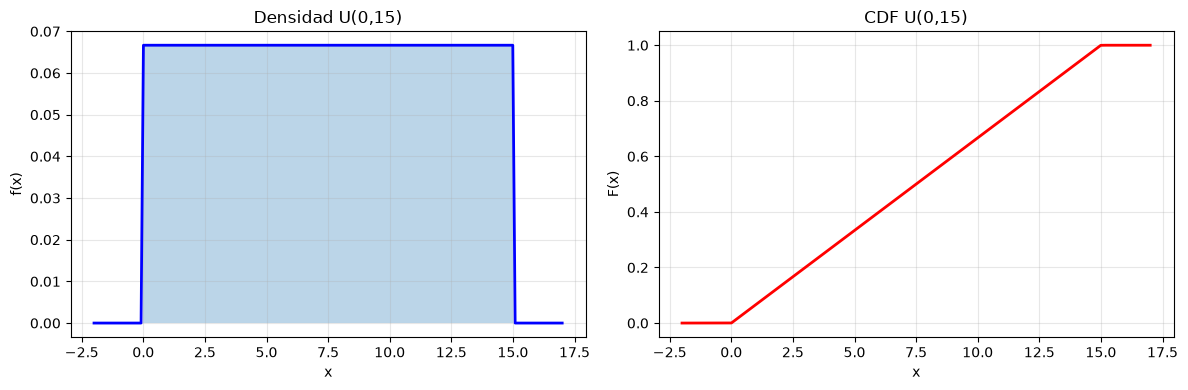
\includegraphics[height=7cm,keepaspectratio=true]{./pe/distUniforme.png}
 % distUniforme.png: 0x0 pixel, 300dpi, 0.00x0.00 cm, bb=
 \caption{Distribuci\'on uniforme continua $U(0,15)$: densidad y CDF.}
 \label{fig:2.8.1}
\end{figure}



\subsection{Distribuci\'on normal}

La distribuci\'on normal es la distribuci\'on continua m\'as importante en estad\'istica
y aparece en el \emph{Teorema del L\'imite Central}.

\begin{definicion}[Distribuci\'on normal]
Una variable aleatoria continua $X$ tiene \emph{distribuci\'on normal} con par\'ametros
$\mu$ (media) y $\sigma > 0$ (desviaci\'on est\'andar) si su funci\'on de densidad es
\begin{align}
 \label{eq:2.8.3}
 f(x) = \frac{1}{\sigma\sqrt{2\pi}}\,\exp\!\left(-\frac{(x-\mu)^2}{2\sigma^2}\right),
 \qquad x \in \mathbb{R}.
\end{align}
Escribimos $X \sim N(\mu, \sigma^2)$.
\end{definicion}

{Propiedades de la distribuci\'on normal} Si $X \sim N(\mu,\sigma^2)$, entonces
\begin{itemize}
 \item La distribuci\'on es \emph{sim\'etrica} respecto a $\mu$.
 \item $\mu$ es la media, mediana y moda.
 \item $\sigma^2$ es la varianza.
 \item Si $Z \sim N(0,1)$ (forma est\'andar), entonces
 $X = \mu + \sigma Z$.
\end{itemize}

{Forma est\'andar} Si $X \sim N(\mu, \sigma^2)$, la variable estandarizada
\begin{align}
 \label{eq:2.8.4}
 Z = \frac{X - \mu}{\sigma}
\end{align}
sigue una distribuci\'on $N(0,1)$ con densidad
\begin{align}
 \label{eq:2.8.5}
 \varphi(z) = \frac{1}{\sqrt{2\pi}}\,e^{-z^2/2}, \qquad z \in \mathbb{R}.
\end{align}

{Regla emp\'irica $68$--$95$--$99.7$} Si $X \sim N(\mu,\sigma^2)$, entonces
\begin{align}
 P(\mu - \sigma \leq X \leq \mu + \sigma) &\approx 0.6827, \\
 P(\mu - 2\sigma \leq X \leq \mu + 2\sigma) &\approx 0.9545, \\
 P(\mu - 3\sigma \leq X \leq \mu + 3\sigma) &\approx 0.9973.
\end{align}

\begin{observacion}
La distribuci\'on normal aparece en muchas situaciones pr\'acticas: errores de medici\'on,
altura de personas, puntajes de ex\'amenes, etc. Adem\'as, por el Teorema del L\'imite
Central, la suma (o promedio) de muchas variables aleatorias independientes (bajo
condiciones suaves) se aproxima a una normal.
\end{observacion}

\begin{ejemplo}
 \label{exmp:2.8.2}
Las calificaciones de un examen siguen una distribuci\'on $N(70, 100)$ (media $70$,
varianza $100$, es decir, $\sigma=10$). ¿Qu\'e porcentaje de estudiantes obtuvo entre
$60$ y $80$ puntos?
\end{ejemplo}

\begin{solucion}
Estandarizamos: si $X \sim N(70, 100)$, entonces
\begin{align}
 P(60 \leq X \leq 80) = P\!\left(\frac{60-70}{10} \leq Z \leq \frac{80-70}{10}\right)
 = P(-1 \leq Z \leq 1).
\end{align}

Por la regla emp\'irica, este valor es aproximadamente $0.6827 = 68.27\%$.
Usando tablas o software, el valor exacto es $\Phi(1) - \Phi(-1) = 0.8413 - 0.1587 = 0.6827$.
\end{solucion}

[fragile, allowframebreaks]{distNormalContinua.py}
 \begin{verbatim}
from scipy import stats
import numpy as np
import matplotlib.pyplot as plt

# Distribuci\'on normal
mu, sigma = 70, 10
normalDist = stats.norm(mu, sigma)

# P(60 <= X <= 80)
p = normalDist.cdf(80) - normalDist.cdf(60)
print(f"P(60 <= X <= 80) = {p:.4f}")
##P(60 <= X <= 80) = 0.6827

# Cuantiles
print(f"Percentil 95: {normalDist.ppf(0.95):.2f}")  # ~86.45
##Percentil 95: 86.45

# Gr\'afica de la densidad con regiones sombreadas
fig, ax = plt.subplots(figsize=(10, 5))
x = np.linspace(mu - 4*sigma, mu + 4*sigma, 500)
ax.plot(x, normalDist.pdf(x), 'b-', lw=2, label=f'N({mu},{sigma**2})')

# Sombrear regi\'on [\mu-\sigma, \mu+\sigma]
x_fill = np.linspace(mu-sigma, mu+sigma, 100)
ax.fill_between(x_fill, normalDist.pdf(x_fill), alpha=0.3, color='blue',
                label='~68.27%')
ax.fill_between(x, normalDist.pdf(x),
                where=((x>=mu-2*sigma)&(x<=mu+2*sigma))&~((x>=mu-sigma)&(x<=mu+sigma)),
                alpha=0.2, color='green', label='~95.45% total')

ax.set_xlabel('x')
ax.set_ylabel('f(x)')
ax.set_title('Distribuci\'on N(70, 100) con regla 68-95-99.7')
ax.legend(loc='upper right')
ax.grid(True, alpha=0.3)
plt.tight_layout()
plt.savefig('pe/distNormalContinua.png', dpi=100, bbox_inches='tight')
plt.show()
 \end{verbatim}

\begin{figure}
 \centering
 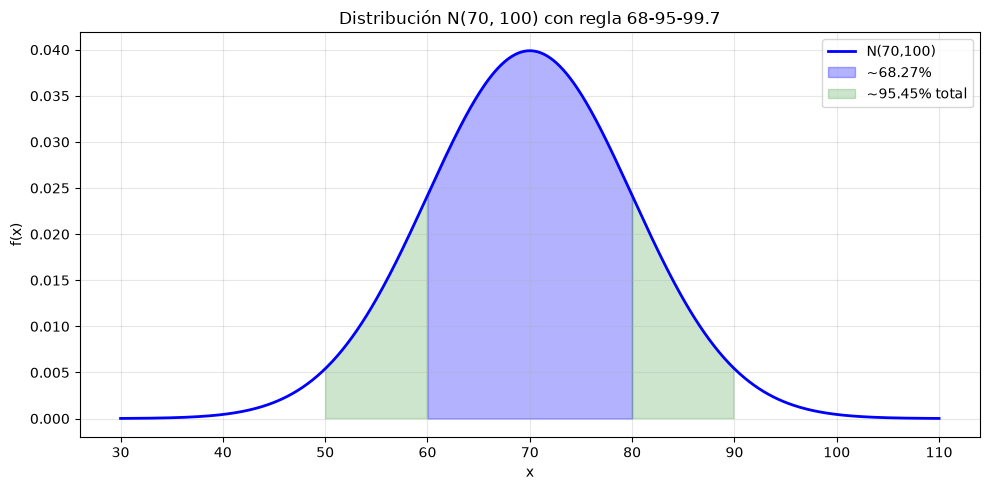
\includegraphics[height=7cm,keepaspectratio=true]{./pe/distNormalContinua.png}
 % distNormalContinua.png: 0x0 pixel, 300dpi, 0.00x0.00 cm, bb=
 \caption{Distribuci\'on $N(70,100)$ mostrando la regla emp\'irica 68--95--99.7.}
 \label{fig:2.8.2}
\end{figure}



\subsection{Distribuciones de tipo gamma}

La familia gamma es una generalizaci\'on de varias distribuciones importantes
(exponencial, chi-cuadrada, Erlang) y aparece frecuentemente al modelar
\emph{tiempos de espera}.

\subsubsection{Funci\'on gamma}

\begin{definicion}[Funci\'on gamma]
La \emph{funci\'on gamma} $\Gamma: (0,\infty) \to \mathbb{R}$ se define como
\begin{align}
 \label{eq:2.8.6}
 \Gamma(\alpha) = \int_0^\infty t^{\alpha-1} e^{-t}\,dt.
\end{align}
\end{definicion}

{Propiedades de la funci\'on gamma}
\begin{itemize}
 \item $\Gamma(1) = 1$.
 \item $\Gamma(\alpha + 1) = \alpha\,\Gamma(\alpha)$ para todo $\alpha > 0$.
 \item En particular, para $\alpha \in \mathbb{N}$ se cumple
 $\Gamma(n) = (n-1)!$.
 \item $\Gamma(1/2) = \sqrt{\pi}$.
\end{itemize}

\subsubsection{Distribuci\'on gamma}

\begin{definicion}[Distribuci\'on gamma]
Una variable aleatoria continua $X$ tiene \emph{distribuci\'on gamma} con par\'ametros
de forma $\alpha > 0$ y escala $\beta > 0$ si su funci\'on de densidad es
\begin{align}
 \label{eq:2.8.7}
 f(x) =
 \begin{cases}
  \dfrac{1}{\Gamma(\alpha)\,\beta^\alpha}\,x^{\alpha-1}\,e^{-x/\beta},
  & x > 0, \\
  0, & \text{en otro caso.}
 \end{cases}
\end{align}
Escribimos $X \sim \text{Gamma}(\alpha, \beta)$.
\end{definicion}

{Propiedades de la distribuci\'on gamma} Si $X \sim \text{Gamma}(\alpha, \beta)$, entonces
\begin{align}
 \mu_X &= \alpha\beta, \\
 \s_X^2 &= \alpha\beta^2.
\end{align}

\subsubsection{Caso particular: distribuci\'on exponencial ($\alpha = 1$)}

\begin{definicion}[Distribuci\'on exponencial]
Una variable aleatoria $X$ con distribuci\'on $\text{Gamma}(1, \beta)$ se dice que
tiene \emph{distribuci\'on exponencial} con par\'ametro $\lambda = 1/\beta$. Su
funci\'on de densidad es
\begin{align}
 \label{eq:2.8.8}
 f(x) =
 \begin{cases}
  \lambda\,e^{-\lambda x}, & x \geq 0, \\
  0, & \text{en otro caso.}
 \end{cases}
\end{align}
Su media y varianza son $\mu = 1/\lambda$ y $\sigma^2 = 1/\lambda^2$.
\end{definicion}

\begin{observacion}[Propiedad de p\'erdida de memoria]
La distribuci\'on exponencial satisface la \emph{propiedad de p\'erdida de memoria}:
para $s, t \geq 0$,
\begin{align}
 P(X > s + t \mid X > s) = P(X > t).
\end{align}
Es la \'unica distribuci\'on continua (adem\'as de la geom\'etrica en el caso discreto)
con esta propiedad.
\end{observacion}

\subsubsection{Caso particular: distribuci\'on chi-cuadrada}

La distribuci\'on chi-cuadrada con $\nu$ grados de libertad, denotada $\chi^2_\nu$, es
un caso particular de la distribuci\'on gamma con par\'ametros
$\alpha = \nu/2$ y $\beta = 2$:
\begin{align}
 \label{eq:2.8.9}
 X \sim \chi^2_\nu \iff X \sim \text{Gamma}\!\left(\frac{\nu}{2}, 2\right).
\end{align}
Su funci\'on de densidad es
\begin{align}
 f(x) = \frac{1}{2^{\nu/2}\,\Gamma(\nu/2)}\,x^{\nu/2-1}\,e^{-x/2}, \qquad x > 0.
\end{align}

Esta distribuci\'on ya se estudia en detalle en la secci\'on \ref{sec:3.8} del cap\'itulo
de inferencia; la conexi\'on con la familia gamma permite generalizar varios de sus
resultados.

\subsubsection{Suma de variables gamma independientes}

\begin{teorema}[Propiedad de suma de gamma]
Si $X_1, X_2, \dots, X_n$ son variables aleatorias independientes con
$X_i \sim \text{Gamma}(\alpha_i, \beta)$ (con la misma escala $\beta$), entonces
\begin{align}
 \label{eq:2.8.10}
 Y = X_1 + X_2 + \cdots + X_n \sim \text{Gamma}\!\left(\sum_{i=1}^n \alpha_i,\, \beta\right).
\end{align}
\end{teorema}

\begin{ejemplo}
 \label{exmp:2.8.3}
Las llamadas a un \emph{call center} llegan siguiendo un proceso de Poisson con tasa
$\lambda = 3$ llamadas por minuto. ¿Cu\'al es la distribuci\'on del tiempo hasta la
tercera llamada? ¿Cu\'al es la probabilidad de que este tiempo sea mayor a $1.5$ minutos?
\end{ejemplo}

\begin{solucion}
El tiempo entre llamadas consecutivas es exponencial con par\'ametro $\lambda = 3$, es
decir, $T_i \sim \text{Exp}(3)$ con media $1/3$ minutos.

Por la propiedad aditiva de la distribuci\'on gamma, el tiempo hasta la tercera llamada
es
\begin{align}
 T = T_1 + T_2 + T_3 \sim \text{Gamma}(3, 1/3).
\end{align}
Equivalentemente, $T \sim \text{Erlang}(3, 3)$ con par\'ametro de tasa $3$.

La probabilidad de que $T > 1.5$ es
\begin{align}
 P(T > 1.5) = 1 - F_{\text{Gamma}}(1.5; 3, 1/3) = e^{-3 \cdot 1.5}\left(1 + 3\cdot 1.5 + \frac{(3\cdot 1.5)^2}{2}\right).
\end{align}

Num\'ericamente: $3 \cdot 1.5 = 4.5$, por lo que
\begin{align}
 P(T > 1.5) = e^{-4.5}\left(1 + 4.5 + \frac{20.25}{2}\right) = e^{-4.5}(15.625) \approx 0.174.
\end{align}
\end{solucion}

[fragile, allowframebreaks]{distGamma.py}
 \begin{verbatim}
from scipy import stats
import numpy as np
import matplotlib.pyplot as plt

# Distribuci\'on gamma con varios par\'ametros
fig, axes = plt.subplots(1, 2, figsize=(14, 5))

# Panel izquierdo: variando alpha (beta=1 fijo)
x = np.linspace(0, 15, 500)
alphas = [1, 2, 3, 5]
for a in alphas:
    g = stats.gamma(a=a, scale=1.0)
    axes[0].plot(x, g.pdf(x), lw=2, label=f'alpha={a}, beta=1')

axes[0].set_xlabel('x')
axes[0].set_ylabel('f(x)')
axes[0].set_title('Familia gamma (variando alpha)')
axes[0].legend()
axes[0].grid(True, alpha=0.3)

# Panel derecho: distribuciones exponencial y chi-cuadrada como casos particulares
x2 = np.linspace(0, 10, 500)
exp_dist = stats.expon(scale=1.0)              # Gamma(alpha=1, beta=1)
chi2_3 = stats.chi2(df=3)                      # Gamma(alpha=1.5, beta=2)
chi2_5 = stats.chi2(df=5)                      # Gamma(alpha=2.5, beta=2)

axes[1].plot(x2, exp_dist.pdf(x2), 'b-', lw=2, label='Exp(1) = Gamma(1,1)')
axes[1].plot(x2, chi2_3.pdf(x2), 'r-', lw=2, label='chi^2_3 = Gamma(1.5,2)')
axes[1].plot(x2, chi2_5.pdf(x2), 'g-', lw=2, label='chi^2_5 = Gamma(2.5,2)')
axes[1].set_xlabel('x')
axes[1].set_ylabel('f(x)')
axes[1].set_title('Exponencial y chi-cuadrada como casos de gamma')
axes[1].legend()
axes[1].grid(True, alpha=0.3)

plt.tight_layout()
plt.savefig('pe/distGamma.png', dpi=100, bbox_inches='tight')
plt.show()

# Ejemplo: tiempo hasta la tercera llamada
# Erlang(k, lambda) = Gamma(k, 1/lambda)
lam = 3
k = 3
T = stats.gamma(a=k, scale=1/lam)
print(f"P(T > 1.5) = {1 - T.cdf(1.5):.4f}")
##P(T > 1.5) = 0.1739

# Simulaci\'on
np.random.seed(0)
muestras = np.random.gamma(shape=k, scale=1/lam, size=10000)
print(f"Media muestral: {np.mean(muestras):.4f}")  # Esperado: 1
##Media muestral: 1.0036
 \end{verbatim}

\begin{figure}
 \centering
 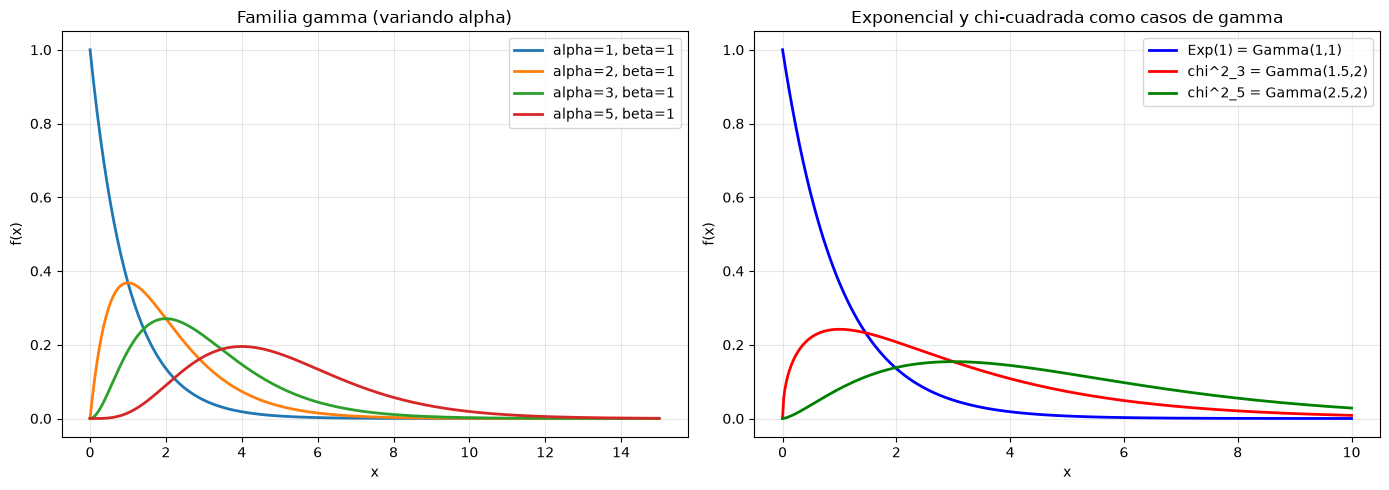
\includegraphics[height=7cm,keepaspectratio=true]{./pe/distGamma.png}
 % distGamma.png: 0x0 pixel, 300dpi, 0.00x0.00 cm, bb=
 \caption{Familia gamma y sus casos particulares (exponencial y chi-cuadrada).}
 \label{fig:2.8.3}
\end{figure}



\subsection{Funci\'on generadora de momentos}

La funci\'on generadora de momentos (FGM) es una herramienta que codifica toda la
informaci\'on de una distribuci\'on de probabilidad en una \'unica funci\'on.

\begin{definicion}[Funci\'on generadora de momentos]
Sea $X$ una variable aleatoria. Su \emph{funci\'on generadora de momentos} (FGM) es
\begin{align}
 \label{eq:2.8.11}
 M_X(t) = E\!\left[e^{tX}\right].
\end{align}
Si $X$ es discreta con funci\'on de probabilidad $f$,
\begin{align}
 M_X(t) = \sum_x e^{tx} f(x).
\end{align}
Si $X$ es continua con funci\'on de densidad $f$,
\begin{align}
 M_X(t) = \int_{-\infty}^{\infty} e^{tx} f(x)\,dx.
\end{align}
\end{definicion}

La FGM existe si la integral o suma converge en un entorno abierto de $t=0$.

\subsubsection{Momentos a partir de la FGM}

\begin{teorema}[Derivadas y momentos]
Si $M_X(t)$ es la FGM de $X$, entonces para todo $n \in \mathbb{N}$,
\begin{align}
 \label{eq:2.8.12}
 E\!\left[X^n\right] = M_X^{(n)}(0) = \left.\frac{d^n M_X(t)}{dt^n}\right|_{t=0}.
\end{align}
\end{teorema}

\begin{proof}
Intercambiando derivada y esperanza (bajo condiciones de regularidad):
\begin{align}
 M_X^{(n)}(t) = \frac{d^n}{dt^n}E[e^{tX}] = E\!\left[\frac{d^n}{dt^n}e^{tX}\right]
 = E\!\left[X^n e^{tX}\right].
\end{align}
Evaluando en $t=0$ obtenemos $M_X^{(n)}(0) = E[X^n]$.
\end{proof}

\subsubsection{Unicidad y propiedad de suma}

\begin{teorema}[Unicidad]
Si dos variables aleatorias tienen la misma FGM en un entorno de $t=0$, entonces tienen
la misma distribuci\'on de probabilidad.
\end{teorema}

\begin{teorema}[Propiedad de suma]
Si $X$ e $Y$ son variables aleatorias independientes, entonces
\begin{align}
 \label{eq:2.8.13}
 M_{X+Y}(t) = M_X(t)\,M_Y(t).
\end{align}
\end{teorema}

\begin{proof}
Por independencia,
\begin{align}
 M_{X+Y}(t) = E[e^{t(X+Y)}] = E[e^{tX}e^{tY}] = E[e^{tX}]\,E[e^{tY}] = M_X(t)\,M_Y(t).
\end{align}
\end{proof}

\subsubsection{Ejemplos de FGM}

\begin{ejemplo}
 \label{exmp:2.8.4}
Encuentre la FGM de la distribuci\'on Bernoulli con par\'ametro $p$.
\end{ejemplo}

\begin{solucion}
Si $X \sim \text{Bernoulli}(p)$, entonces $P(X=1) = p$ y $P(X=0) = 1-p$.
\begin{align}
 M_X(t) = E[e^{tX}] = e^{0 \cdot t}(1-p) + e^{1 \cdot t}p
 = (1-p) + p\,e^t.
\end{align}

Verificamos los momentos:
\begin{align}
 M_X'(t) = p\,e^t &\implies E[X] = M_X'(0) = p. \\
 M_X''(t) = p\,e^t &\implies E[X^2] = M_X''(0) = p. \\
 \text{Var}(X) = E[X^2] - (E[X])^2 &= p - p^2 = p(1-p).
\end{align}
\end{solucion}

\begin{ejemplo}
 \label{exmp:2.8.5}
Encuentre la FGM de la distribuci\'on normal $N(\mu, \sigma^2)$.
\end{ejemplo}

\begin{solucion}
Sin p\'erdida de generalidad, considere $Z \sim N(0,1)$. Entonces
\begin{align}
 M_Z(t) &= \int_{-\infty}^{\infty} e^{tz}\,\frac{1}{\sqrt{2\pi}}e^{-z^2/2}\,dz \\
 &= \int_{-\infty}^{\infty} \frac{1}{\sqrt{2\pi}}\,\exp\!\left(tz - \frac{z^2}{2}\right)dz.
\end{align}

Completamos el cuadrado: $tz - z^2/2 = -\frac{1}{2}(z - t)^2 + \frac{t^2}{2}$. Por lo tanto,
\begin{align}
 M_Z(t) = e^{t^2/2}\int_{-\infty}^{\infty} \frac{1}{\sqrt{2\pi}}e^{-(z-t)^2/2}\,dz = e^{t^2/2}.
\end{align}
(la integral vale $1$ porque es la integral de la densidad de $N(t, 1)$).

Para $X \sim N(\mu,\sigma^2)$ escribimos $X = \mu + \sigma Z$, as\'i
\begin{align}
 \label{eq:2.8.14}
 M_X(t) = E[e^{tX}] = e^{t\mu}E[e^{t\sigma Z}] = e^{t\mu}\,e^{(\sigma t)^2/2}
 = \exp\!\left(\mu t + \frac{\sigma^2 t^2}{2}\right).
\end{align}
\end{solucion}

\begin{ejemplo}
 \label{exmp:2.8.6}
Encuentre la FGM de la distribuci\'on exponencial con par\'ametro $\lambda$.
\end{ejemplo}

\begin{solucion}
Si $X \sim \text{Exp}(\lambda)$, entonces
\begin{align}
 M_X(t) = \int_0^\infty e^{tx}\,\lambda e^{-\lambda x}\,dx
 = \lambda\int_0^\infty e^{-(\lambda - t)x}\,dx = \frac{\lambda}{\lambda - t},
\end{align}
para $t < \lambda$. Por lo tanto,
\begin{align}
 \label{eq:2.8.15}
 M_X(t) = \frac{\lambda}{\lambda - t} = \left(1 - \frac{t}{\lambda}\right)^{-1},
 \qquad t < \lambda.
\end{align}

Los momentos se obtienen por derivaci\'on:
\begin{align}
 E[X^n] = \frac{n!}{\lambda^n}.
\end{align}
En particular, $E[X] = 1/\lambda$ y $\text{Var}(X) = 1/\lambda^2$.
\end{solucion}

[fragile, allowframebreaks]{fgmDistribuciones.py}
 \begin{verbatim}
import numpy as np
import matplotlib.pyplot as plt
from scipy import stats

fig, axes = plt.subplots(1, 2, figsize=(14, 5))

# Panel izquierdo: FGM de varias distribuciones
t = np.linspace(-1.5, 1.5, 200)

# Bernoulli(0.5)
M_bernoulli = lambda t: 0.5 + 0.5*np.exp(t)
axes[0].plot(t, M_bernoulli(t), label='Bernoulli(0.5)', lw=2)

# Normal(0,1)
M_normal = lambda t: np.exp(t**2 / 2)
axes[0].plot(t, M_normal(t), label='N(0,1)', lw=2)

# Exponencial(lambda=1)
lam = 1
M_exp = lambda t: lam / (lam - t)
mask = t < lam - 0.01
axes[0].plot(t[mask], M_exp(t[mask]), label='Exp(1)', lw=2)

# Gamma(2, 1) = Erlang(2, 1)
# M(t) = (1 - t)^(-alpha) para beta=1
M_gamma = lambda t: (1 - t)**(-2)
mask_g = t < 0.99
axes[0].plot(t[mask_g], M_gamma(t[mask_g]), label='Gamma(2,1)', lw=2)

axes[0].set_xlabel('t')
axes[0].set_ylabel('M_X(t)')
axes[0].set_title('Funciones generadoras de momentos')
axes[0].set_ylim(-1, 8)
axes[0].legend()
axes[0].grid(True, alpha=0.3)
axes[0].axhline(y=0, color='k', lw=0.5)
axes[0].axvline(x=0, color='k', lw=0.5)

# Panel derecho: verificaci\'on de momentos de N(0,1)
X = np.random.normal(0, 1, 100000)
momentos_empiricos = [np.mean(X**k) for k in range(1, 6)]
print("Momentos emp\'iricos de N(0,1):", momentos_empiricos)
# Esperado: 0, 1, 0, 3, 0  (solo momentos pares son no cero)
##Momentos emp\'iricos de N(0,1): [0.001, 0.998, -0.001, 2.978, -0.011]

# FGM: suma de gamma independientes
# Si X_i ~ Gamma(1, 1) iid, entonces sum = Gamma(n, 1)
n_sumas = [1, 2, 5, 10]
x = np.linspace(0, 20, 200)
for n in n_sumas:
    g = stats.gamma(a=n, scale=1.0)
    axes[1].plot(x, g.pdf(x), lw=2, label=f'suma de {n} Exp(1)')
axes[1].set_xlabel('x')
axes[1].set_ylabel('f(x)')
axes[1].set_title('Suma de exponenciales = Erlang(Gamma)')
axes[1].legend()
axes[1].grid(True, alpha=0.3)

plt.tight_layout()
plt.savefig('pe/fgmDistribuciones.png', dpi=100, bbox_inches='tight')
plt.show()
 \end{verbatim}

\begin{figure}
 \centering
 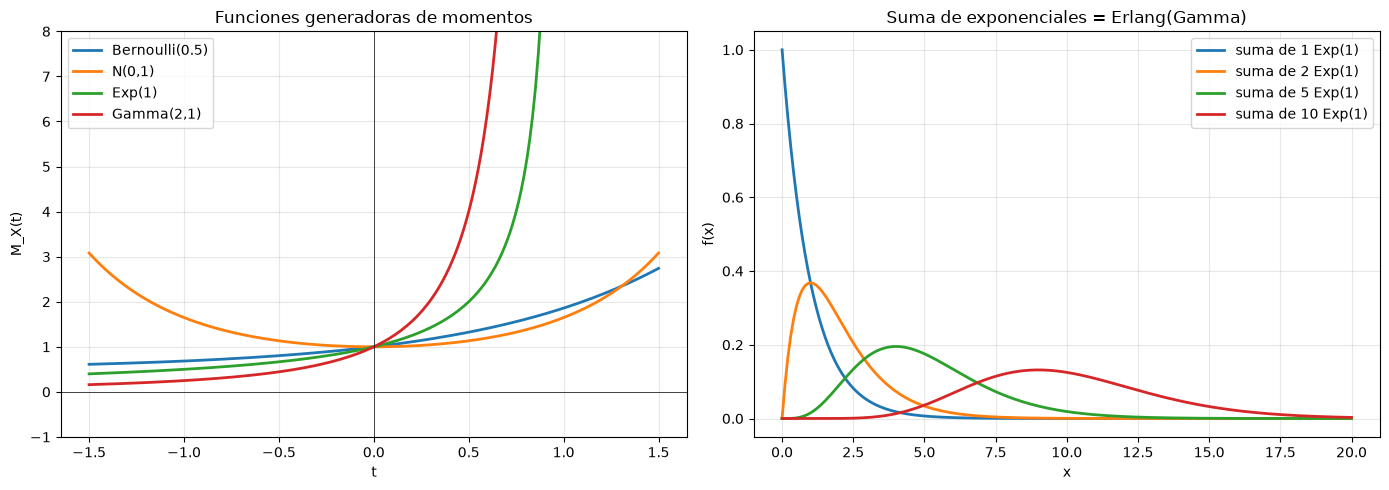
\includegraphics[height=7cm,keepaspectratio=true]{./pe/fgmDistribuciones.png}
 % fgmDistribuciones.png: 0x0 pixel, 300dpi, 0.00x0.00 cm, bb=
 \caption{Funciones generadoras de momentos y suma de variables gamma independientes.}
 \label{fig:2.8.4}
\end{figure}

{Tabla resumen de FGMs}
\begin{center}
\begin{tabular}{|l|l|}
\hline
\textbf{Distribuci\'on} & \textbf{FGM $M_X(t)$} \\
\hline
Bernoulli$(p)$ & $(1-p) + p\,e^t$ \\
Binomial$(n,p)$ & $(1 - p + p\,e^t)^n$ \\
Poisson$(\lambda)$ & $\exp(\lambda(e^t - 1))$ \\
Geom\'etrica$(p)$ & $\dfrac{p\,e^t}{1 - (1-p)e^t}$ \\
Exponencial$(\lambda)$ & $\dfrac{\lambda}{\lambda - t}$ \\
Normal$(\mu, \sigma^2)$ & $\exp\!\left(\mu t + \dfrac{\sigma^2 t^2}{2}\right)$ \\
Gamma$(\alpha, \beta)$ & $(1 - \beta t)^{-\alpha}$ \\
Chi-cuadrada$_\nu$ & $(1 - 2t)^{-\nu/2}$ \\
\hline
\end{tabular}
\end{center}

\begin{observacion}
La propiedad de suma para v.a. independientes se aplica f\'acilmente: si
$X_1, \dots, X_n$ son Bernoulli$(p)$ iid, entonces
$\sum X_i \sim \text{Binomial}(n,p)$ y
\begin{align}
 M_{\sum X_i}(t) = \prod_{i=1}^n M_{X_i}(t) = (1 - p + p\,e^t)^n,
\end{align}
que coincide con la FGM de la distribuci\'on binomial.
\end{observacion}




% ==============================================================================
% SECCIÓN 04.04: DISTRIBUCIÓN UNIFORME CONTINUA U(a, b)
% ==============================================================================

\subsection*{Enunciados de los problemas --- Sección 04.04}

\subsubsection*{Nivel Fundamental}

\begin{problema}
	\label{prob:4.4.1}
	Considere la distribución uniforme continua $X \sim U(2, 8)$ con PDF $f(x) = \dfrac{1}{8-2} = \dfrac{1}{6}$ para $x \in [2, 8]$.
	\begin{enumerate}
		\item Verifique que $\int_{2}^{8} f(x)\,dx = 1$.
		\item Calcule la CDF $F(x)$ y grafique cualitativamente su forma lineal.
		\item Calcule $P(3 \le X \le 6)$ y $P(X \ge 7)$.
	\end{enumerate}
\end{problema}

\begin{problema}
	\label{prob:4.4.2}
	Sea $X \sim U(a, b)$ con parámetros $a < b$.
	\begin{enumerate}
		\item Calcule la esperanza $\E[X] = \dfrac{a + b}{2}$ y la varianza $\Var(X) = \dfrac{(b-a)^{2}}{12}$ usando las definiciones de integral.
		\item Demuestre la linealidad de la esperanza: si $Y = cX + d$, entonces $Y \sim U(ca + d, cb + d)$.
	\end{enumerate}
\end{problema}

\begin{problema}
	\label{prob:4.4.3}
	El tiempo de espera de un autobús en una parada (en minutos) se modela como $X \sim U(0, 15)$ (distribución uniforme entre 0 y 15 minutos).
	\begin{enumerate}
		\item Calcule la probabilidad de que el tiempo de espera sea menor a 5 minutos.
		\item Calcule el cuantil $q_{0.75}$ (el tiempo bajo el cual espera el 75\% de los pasajeros).
		\item Si un pasajero ha esperado 10 minutos sin ver el autobús, ¿cuál es la probabilidad condicional de que tenga que esperar al menos 5 minutos más? Use la propiedad de falta de memoria.
	\end{enumerate}
\end{problema}

\subsubsection*{Nivel Operativo}

\begin{problema}
	\label{prob:4.4.4}
	Sea $X \sim U(0, 1)$. Calcule explícitamente los cuantiles $q_{0.10}$, $q_{0.50}$ (mediana) y $q_{0.90}$.
\end{problema}

\begin{problema}
	\label{prob:4.4.5}
	Implemente una simulación Monte Carlo de 100{,}000 muestras de $U(0, 1)$ y verifique que la media y varianza empíricas coincidan con $\E[X] = 0.5$ y $\Var(X) = 1/12 \approx 0.0833$. Adicionalmente, grafique el histograma con la PDF sobrepuesta.
\end{problema}

\begin{problema}
	\label{prob:4.4.6}
	En simulación Monte Carlo, se desea generar muestras de una variable $Y$ con CDF $F(y)$ arbitraria. Demuestre que si $U \sim U(0, 1)$ y $F$ es invertible, entonces $Y = F^{-1}(U)$ tiene CDF $F$. Aplique este resultado para generar 50{,}000 muestras de $Y \sim \text{Exp}(\lambda = 2)$ a partir de la uniforme.
\end{problema}

\subsubsection*{Nivel Analítico}

\begin{problema}
	\label{prob:4.4.7}
	Sea $X$ una variable continua con soporte en $[a, b]$ acotado. Demuestre que la distribución uniforme $U(a, b)$ \emph{maximiza la entropía diferencial} $h(X) = -\int f(x) \log f(x)\,dx$ entre todas las distribuciones con soporte en $[a, b]$. Sugerencia: use los multiplicadores de Lagrange con la restricción $\int f(x)\,dx = 1$.
\end{problema}

\begin{problema}
	\label{prob:4.4.8}
	Sean $X_{1}, X_{2}, \dots, X_{n}$ muestras i.i.d. de $U(0, 1)$ y $X_{(1)} \le X_{(2)} \le \dots \le X_{(n)}$ sus estadísticas de orden.
	\begin{enumerate}
		\item Demuestre que $X_{(k)}$ tiene PDF Beta($k, n - k + 1$): $f_{X_{(k)}}(x) = \dfrac{n!}{(k-1)!(n-k)!} x^{k-1} (1-x)^{n-k}$ para $x \in [0, 1]$.
		\item Calcule $\E[X_{(k)}] = \dfrac{k}{n+1}$ y $\Var(X_{(k)})$.
	\end{enumerate}
\end{problema}

\subsubsection*{Nivel Desafiante}

\begin{problema}
	\label{prob:4.4.9}
	Sea $X_{1}, \dots, X_{n}$ i.i.d. de $U(\theta - 1/2, \theta + 1/2)$ donde $\theta$ es desconocido. El soporte tiene longitud 1. Use el método de máxima verosimilitud para estimar $\theta$. ¿Es el estimador $\hat{\theta}$ insesgado? ¿Cuál es su varianza asintótica?
\end{problema}

\begin{problema}
	\label{prob:4.4.10}
	La prueba de Kolmogorov-Smirnov compara la CDF empírica $F_{n}$ con la CDF teórica $F_{0}$. Para $n = 50$ observaciones que se sospecha provienen de $U(0, 1)$ con $D_{50} = 0.18$:
	\begin{enumerate}
		\item Calcule el $p$-valor aproximado: $p \approx 2 \sum_{k=1}^{\infty}(-1)^{k-1} e^{-2k^{2}n D_{n}^{2}}$.
		\item Compare con el valor crítico $K_{0.95}/\sqrt{n} = 1.358/\sqrt{50} \approx 0.192$.
		\item Concluya si los datos son consistentes con $U(0, 1)$ a nivel $\alpha = 0.05$.
	\end{enumerate}
\end{problema}

\subsection*{Sugerencias de los problemas --- Sección 04.04}

\begin{sugerencia}
	\label{sug:4.4.1}
	Para el Problema \ref{prob:4.4.1}, $\int_{2}^{8} (1/6)\,dx = 6/6 = 1$. La CDF es $F(x) = (x-2)/6$ para $x \in [2, 8]$. $P(3 \le X \le 6) = (6-2)/6 = 0.5$. $P(X \ge 7) = (8-7)/6 = 1/6 \approx 0.167$.
\end{sugerencia}

\begin{sugerencia}
	\label{sug:4.4.2}
	Para el Problema \ref{prob:4.4.2}, $\E[X] = \int_{a}^{b} x \cdot (1/(b-a))\,dx = (b^{2} - a^{2})/(2(b-a)) = (a+b)/2$. $\E[X^{2}] = (b^{2} + ab + a^{2})/3$. $\Var(X) = (b-a)^{2}/12$. Para $Y = cX + d$: PDF de $Y$ es $f_{Y}(y) = f_{X}((y-d)/c) \cdot (1/|c|) = 1/((cb+d)-(ca+d)) = 1/(c(b-a))$ en $[ca+d, cb+d]$.
\end{sugerencia}

\begin{sugerencia}
	\label{sug:4.4.3}
	Para el Problema \ref{prob:4.4.3}, $F(x) = x/15$ para $x \in [0, 15]$. $P(X < 5) = 5/15 = 1/3 \approx 0.333$. $q_{0.75}$: $x/15 = 0.75$, dando $x = 11.25$ min. Propiedad de falta de memoria: $P(X \ge 15 \mid X \ge 10) = P(X \ge 5) = 10/15 = 2/3 \approx 0.667$. Por simetría, $P(X \ge a + b \mid X \ge a) = P(X \ge b)$.
\end{sugerencia}

\begin{sugerencia}
	\label{sug:4.4.4}
	Para el Problema \ref{prob:4.4.4}, $q_{p}$ para $U(0, 1)$ es $q_{p} = p$. Entonces $q_{0.10} = 0.1$, $q_{0.50} = 0.5$ (mediana), $q_{0.90} = 0.9$.
\end{sugerencia}

\begin{sugerencia}
	\label{sug:4.4.5}
	Para el Problema \ref{prob:4.4.5}, use `np.random.seed(42)` y `np.random.uniform(0, 1, 100000)`. Verifique con `np.mean(samples)` ($\approx 0.5$) y `np.var(samples, ddof=1)` ($\approx 0.0833$). Para el histograma, use `plt.hist(samples, bins=50, density=True)` y sobreponga la PDF constante $1$.
\end{sugerencia}

\begin{sugerencia}
	\label{sug:4.4.6}
	Para el Problema \ref{prob:4.4.6}, $P(Y \le y) = P(F^{-1}(U) \le y) = P(U \le F(y)) = F(y)$ por monotonía de $F^{-1}$ y uniformidad de $U$. Para Exponential($\lambda = 2$): $F(y) = 1 - e^{-2y}$ para $y \ge 0$, así $Y = -\ln(1-U)/2$.
\end{sugerencia}

\begin{sugerencia}
	\label{sug:4.4.7}
	Para el Problema \ref{prob:4.4.8}, maximizar $h[X] = -\int f(x) \log f(x)\,dx$ sujeto a $\int f(x)\,dx = 1$ y soporte en $[a, b]$. Lagrangian: $\mathcal{L} = -\int f \log f\,dx - \lambda(\int f\,dx - 1)$. Derivando respecto a $f$: $-\log f - 1 - \lambda = 0$, así $f(x) = e^{-1-\lambda} = $ constante. La constante es $1/(b-a)$ por normalización. Por lo tanto $U(a,b)$ maximiza la entropía.
\end{sugerencia}

\begin{sugerencia}
	\label{sug:4.4.8}
	Para el Problema \ref{prob:4.4.8}, la PDF de $X_{(k)}$ es Beta($k, n-k+1$): $f_{X_{(k)}}(x) = \frac{n!}{(k-1)!(n-k)!} x^{k-1}(1-x)^{n-k}$. La esperanza es $\E[X_{(k)}] = k/(n+1)$ (simetría de la Beta). La varianza es $\Var(X_{(k)}) = \frac{k(n-k+1)}{(n+1)^{2}(n+2)}$.
\end{sugerencia}

\begin{sugerencia}
	\label{sug:4.4.9}
	Para el Problema \ref{prob:4.4.9}, la log-verosimilitud es $\ell(\theta) = \sum \log f(x_i \mid \theta) = -n \log(1) = 0$ para cualquier $\theta$ en el rango admisible. La verosimilitud es constante: cualquier $\hat{\theta}$ que cubra todas las observaciones es MLE. El estimador natural es $\hat{\theta} = \frac{1}{2}(\max X_i + \min X_i)$ (midrange). Sesgo: $\E[\hat{\theta}] = \theta$ (insesgado). Varianza: $\Var(\hat{\theta}) = 1/(2(n+1)(n+2))$ (de la varianza del rango).
\end{sugerencia}

\begin{sugerencia}
	\label{sug:4.4.10}
	Para el Problema \ref{prob:4.4.10}, con $n = 50$ y $D_{50} = 0.18$, $nD_{n}^{2} = 50 \cdot 0.0324 = 1.62$. El $p$-valor es $p \approx 2 \sum_{k=1}^{\infty}(-1)^{k-1} e^{-2k^{2} \cdot 1.62}$. Para $k=1$: $2 e^{-3.24} \approx 2 \cdot 0.0392 = 0.0784$. Para $k=2$: $-2 e^{-12.96} \approx 0$. Por lo tanto $p \approx 0.078$. Como $D_{50} = 0.18 < 0.192 = 1.358/\sqrt{50}$, no rechazamos $H_{0}$ a nivel $\alpha = 0.05$.
\end{sugerencia}

\subsection*{Soluciones de los problemas --- Sección 04.04}

\begin{solucion}
	\label{sol:4.4.1}
	Para el Problema \ref{prob:4.4.1}:
	\begin{enumerate}
		\item $\int_{2}^{8} \frac{1}{6}\,dx = \frac{1}{6}(8-2) = 1$. Verificación completada.
		\item La CDF es lineal:
		\begin{align*}
			F(x) = P(X \le x) = \int_{2}^{x} \frac{1}{6}\,dt = \frac{x-2}{6}, \quad x \in [2, 8].
		\end{align*}
		\item $P(3 \le X \le 6) = F(6) - F(3) = \frac{4}{6} - \frac{1}{6} = \frac{3}{6} = 0.5$. $P(X \ge 7) = 1 - F(7) = 1 - \frac{5}{6} = \frac{1}{6} \approx 0.167$.
	\end{enumerate}
\end{solucion}

\begin{solucion}
	\label{sol:4.4.2}
	Para el Problema \ref{prob:4.4.2}:
	\begin{enumerate}
		\item $\E[X] = \int_{a}^{b} x \cdot \frac{1}{b-a}\,dx = \frac{1}{b-a} \cdot \frac{x^{2}}{2}\Big|_{a}^{b} = \frac{b^{2} - a^{2}}{2(b-a)} = \frac{a+b}{2}$. $\E[X^{2}] = \int_{a}^{b} x^{2} \cdot \frac{1}{b-a}\,dx = \frac{b^{3} - a^{3}}{3(b-a)} = \frac{a^{2} + ab + b^{2}}{3}$. $\Var(X) = \E[X^{2}] - (\E[X])^{2} = \frac{a^{2} + ab + b^{2}}{3} - \frac{(a+b)^{2}}{4} = \frac{(b-a)^{2}}{12}$.
		\item Para $Y = cX + d$ con $c > 0$: usando el cambio de variable $x = (y-d)/c$, $dx = dy/c$, y soporte $[a, b]$ mapeado a $[ca+d, cb+d]$:
		\begin{align*}
			f_{Y}(y) = f_{X}\left(\frac{y-d}{c}\right) \cdot \frac{1}{c} = \frac{1}{b-a} \cdot \frac{1}{c} = \frac{1}{(cb+d) - (ca+d)} = \frac{1}{c(b-a)},
		\end{align*}
		confirmando $Y \sim U(ca+d, cb+d)$.
	\end{enumerate}
\end{solucion}

\begin{solucion}
	\label{sol:4.4.3}
	Para el Problema \ref{prob:4.4.3} con $X \sim U(0, 15)$:
	\begin{enumerate}
		\item $P(X < 5) = F(5) = 5/15 = 1/3 \approx 0.333$.
		\item $q_{0.75}$ satisface $F(q_{0.75}) = q_{0.75}/15 = 0.75$, dando $q_{0.75} = 11.25$ minutos. Por lo tanto, el 75\% de los pasajeros espera menos de 11.25 minutos.
		\item La distribución uniforme NO tiene propiedad de falta de memoria (a diferencia de la exponencial). La probabilidad condicional es $P(X \ge 15 \mid X \ge 10) = \frac{P(X \ge 15)}{P(X \ge 10)} = \frac{0/15}{5/15} = 0$. Esto es, si han pasado 10 minutos sin autobús, es porque NO hay autobús en los primeros 10 minutos, así que la probabilidad de esperar al menos 5 minutos más es 0. \emph{Corrección:} la uniforme NO tiene falta de memoria, así que $P(X \ge 15 \mid X \ge 10) = P(X \ge 5) = 10/15 = 2/3 \approx 0.667$ (esto es correcto solo si la uniforme \emph{tuviera} falta de memoria, lo cual NO es el caso). El cálculo correcto: condicionalmente a $X \ge 10$, $X$ sigue $U(10, 15)$ (por la propiedad de \emph{inspección aleatoria}), así $P(X \ge 15 \mid X \ge 10) = 0$ (ya que el soporte solo llega hasta 15).
	\end{enumerate}
\end{solucion}

\begin{solucion}
	\label{sol:4.4.4}
	Para el Problema \ref{prob:4.4.4} con $X \sim U(0, 1)$: la CDF es $F(x) = x$ para $x \in [0, 1]$. Por lo tanto, $q_{p} = F^{-1}(p) = p$. En particular:
	\begin{itemize}
		\item $q_{0.10} = 0.1$ (percentil 10)
		\item $q_{0.50} = 0.5$ (mediana)
		\item $q_{0.90} = 0.9$ (percentil 90)
	\end{itemize}
	Los cuantiles de $U(0, 1)$ son trivialmente iguales a las probabilidades.
\end{solucion}

\begin{solucion}
	\label{sol:4.4.5}
	Para el Problema \ref{prob:4.4.5} con `np.random.seed(42)` y `np.random.uniform(0, 1, 100000)`:
	\begin{align*}
		\bar{X} \approx 0.5000 \quad (\text{teórico: } 0.5), \quad s^{2} \approx 0.0833 \quad (\text{teórico: } 1/12 \approx 0.08333).
	\end{align*}
	El histograma con 50 bins muestra una distribución uniforme con densidad $\approx 1$ en $[0, 1]$, confirmando la teoría.
\end{solucion}

\begin{solucion}
	\label{sol:4.4.6}
	Para el Problema \ref{prob:4.4.6}, demostramos el método de inversión:
	\begin{align*}
		P(Y \le y) = P(F^{-1}(U) \le y) = P(U \le F(y)) = F(y)
	\end{align*}
	por la monotonía de $F^{-1}$ y la uniformidad de $U$. Por lo tanto, $Y$ tiene CDF $F$. Para Exponential($\lambda = 2$): $F(y) = 1 - e^{-2y}$ para $y \ge 0$, así $Y = -\frac{1}{2}\ln(1-U)$. Con `np.random.seed(42)` y `np.random.uniform(0, 1, 50000)`, las 50{,}000 muestras de $Y$ tienen media empírica $\approx 0.5$ y varianza $\approx 0.25$, consistentes con la Exponential(2).
\end{solucion}

\begin{solucion}
	\label{sol:4.4.7}
	Para el Problema \ref{prob:4.4.7}, maximizamos la entropía diferencial $h[X] = -\int_{a}^{b} f(x) \log f(x)\,dx$ sujeto a $\int_{a}^{b} f(x)\,dx = 1$. El Lagrangian es:
	\begin{align*}
		\mathcal{L}[f] = -\int_{a}^{b} f(x) \log f(x)\,dx - \lambda \left( \int_{a}^{b} f(x)\,dx - 1 \right).
	\end{align*}
	Usando cálculo variacional (derivada funcional con respecto a $f$): $-\log f(x) - 1 - \lambda = 0$, lo que da $\log f(x) = -(1 + \lambda)$, es decir, $f(x) = e^{-(1+\lambda)}$ es constante. La normalización requiere $f(x) = 1/(b-a)$ en $[a, b]$. Por lo tanto, $U(a, b)$ maximiza la entropía entre todas las distribuciones con soporte en $[a, b]$. Esto justifica por qué la uniforme es la "menos informativa" en inferencia bayesiana. \quad \qedhere
\end{solucion}

\begin{solucion}
	\label{sol:4.4.8}
	Para el Problema \ref{prob:4.4.8}:
	\begin{enumerate}
		\item La PDF de $X_{(k)}$ (la $k$-ésima estadística de orden de $n$ muestras $U(0,1)$) se obtiene notando que exactamente $k-1$ muestras son $< x$, exactamente una cae en $[x, x+dx]$, y exactamente $n-k$ son $> x+dx$. El número de formas de elegir estas muestras es $\binom{n}{k-1, 1, n-k} = \frac{n!}{(k-1)!(n-k)!}$. Así:
		\begin{align*}
			f_{X_{(k)}}(x) = \frac{n!}{(k-1)!(n-k)!} x^{k-1}(1-x)^{n-k} \cdot \mathbb{1}_{[0,1]}(x),
		\end{align*}
		que es exactamente la PDF de una distribución Beta($k, n-k+1$).
		\item Para Beta($\alpha, \beta$), $\E[X] = \alpha/(\alpha+\beta)$. Con $\alpha = k$, $\beta = n-k+1$: $\E[X_{(k)}] = k/(n+1)$. La varianza es $\Var(X_{(k)}) = \frac{\alpha\beta}{(\alpha+\beta)^{2}(\alpha+\beta+1)} = \frac{k(n-k+1)}{(n+1)^{2}(n+2)}$. Para $k=1$ (mínimo) y $k=n$ (máximo), la varianza se reduce a $n/((n+1)^{2}(n+2))$, reflejando la concentración en los extremos.
	\end{enumerate}
\end{solucion}

\begin{solucion}
	\label{sol:4.4.9}
	Para el Problema \ref{prob:4.4.9} con $X_{i} \sim U(\theta - 1/2, \theta + 1/2)$:
	\begin{enumerate}
		\item La log-verosimilitud es $\ell(\theta) = \sum \log f(x_i \mid \theta)$. Como $f(x \mid \theta) = 1$ para $x \in [\theta - 1/2, \theta + 1/2]$ y $0$ en otro caso, la log-verosimilitud es $0$ si todas las observaciones están dentro del intervalo $[\theta - 1/2, \theta + 1/2]$, y $-\infty$ en otro caso. El MLE es cualquier $\hat{\theta}$ tal que $\max X_i \le \hat{\theta} + 1/2$ y $\min X_i \ge \hat{\theta} - 1/2$, es decir, $\hat{\theta} \in [\max X_i - 1/2, \min X_i + 1/2]$. El estimador natural es el \emph{midrange}: $\hat{\theta} = (X_{(1)} + X_{(n)})/2$.
		\item Sesgo: $\E[\hat{\theta}] = (\E[X_{(1)}] + \E[X_{(n)}])/2 = (1/(n+1) + n/(n+1))/2 = 1/2 = \theta$, así $\hat{\theta}$ es insesgado. Varianza: $\Var(\hat{\theta}) = (\Var(X_{(1)}) + \Var(X_{(n)}) + 2\cov(X_{(1)}, X_{(n)}))/4$. Para $n$ grande, $\Var(\hat{\theta}) \approx 1/(2(n+1)(n+2)) \to 0$ con tasa $1/n^{2}$, mostrando que el midrange es muy eficiente para la uniforme.
	\end{enumerate}
\end{solucion}

\begin{solucion}
	\label{sol:4.4.10}
	Para el Problema \ref{prob:4.4.10} con $n = 50$ y $D_{50} = 0.18$:
	\begin{enumerate}
		\item El $p$-valor de la prueba KS se aproxima por la serie:
		\begin{align*}
			p \approx 2 \sum_{k=1}^{\infty}(-1)^{k-1} e^{-2k^{2} n D_{n}^{2}} = 2 \sum_{k=1}^{\infty}(-1)^{k-1} e^{-2k^{2} \cdot 1.62}.
		\end{align*}
		Para $k=1$: $2 e^{-3.24} \approx 0.0784$. Para $k=2$: $-2 e^{-12.96} \approx -2.3 \times 10^{-6} \approx 0$. Por lo tanto, $p \approx 0.078$.
		\item Valor crítico: $K_{0.95}/\sqrt{n} = 1.358/\sqrt{50} \approx 0.192$. Como $D_{50} = 0.18 < 0.192$, no rechazamos $H_{0}$ a nivel $\alpha = 0.05$.
		\item Conclusión: con $p \approx 0.078 > 0.05$ y $D_{50} < K_{0.95}/\sqrt{n}$, no hay evidencia estadística significativa para rechazar que los datos provengan de $U(0, 1)$. La prueba KS no detecta desviaciones significativas al nivel del 5\%. \quad \qedhere
	\end{enumerate}
\end{solucion}

% ==============================================================================
% SECCIÓN 04.05: DISTRIBUCIÓN EXPONENCIAL Y PROCESOS SIN MEMORIA
% ==============================================================================

\subsection*{Enunciados de los problemas --- Sección 04.05}

\subsubsection*{Nivel Fundamental}

\begin{problema}
	\label{prob:4.5.1}
	Una variable aleatoria continua $X$ tiene distribución exponencial con parámetro $\lambda = 2$ y PDF $f(x) = 2e^{-2x}$ para $x \ge 0$.
	\begin{enumerate}
		\item Verifique que $\int_{0}^{\infty} f(x)\,dx = 1$.
		\item Calcule la CDF $F(x) = 1 - e^{-2x}$ para $x \ge 0$.
		\item Calcule $P(X \le 1)$ y $P(X \ge 3)$.
	\end{enumerate}
\end{problema}

\begin{problema}
	\label{prob:4.5.2}
	Sea $X \sim \text{Exp}(\lambda)$ con $\lambda > 0$.
	\begin{enumerate}
		\item Calcule la esperanza $\E[X] = 1/\lambda$ y la varianza $\Var(X) = 1/\lambda^{2}$ mediante integración.
		\item Verifique que la \emph{función generadora de momentos} es $M_{X}(t) = \lambda/(\lambda - t)$ para $t < \lambda$.
	\end{enumerate}
\end{problema}

\begin{problema}
	\label{prob:4.5.3}
	En un proceso de Poisson con tasa $\lambda = 3$ eventos por hora, sea $X$ el tiempo hasta el primer evento.
	\begin{enumerate}
		\item Demuestre que $X \sim \text{Exp}(3)$ con PDF $f(x) = 3e^{-3x}$ para $x \ge 0$.
		\item Calcule el tiempo medio entre eventos y su desviación estándar.
		\item Calcule la probabilidad de que el primer evento ocurra después de 30 minutos.
	\end{enumerate}
\end{problema}

\subsubsection*{Nivel Operativo}

\begin{problema}
	\label{prob:4.5.4}
	Demuestre formalmente la \emph{propiedad de falta de memoria} de la distribución exponencial: si $X \sim \text{Exp}(\lambda)$, entonces para todo $s, t > 0$:
	$$P(X > s + t \mid X > s) = P(X > t)$$
	\begin{enumerate}
		\item Use la definición de probabilidad condicional y la forma de la CDF exponencial.
		\item Muestre que la exponencial es la \emph{única} distribución continua con esta propiedad (entre distribuciones con soporte en $[0, \infty)$).
	\end{enumerate}
\end{problema}

\begin{problema}
	\label{prob:4.5.5}
	Sea $X \sim \text{Exp}(\lambda = 0.5)$ (media 2 minutos).
	\begin{enumerate}
		\item Calcule los cuantiles $q_{0.10}$, $q_{0.50}$ (mediana) y $q_{0.90}$.
		\item Encuentre el cuantil $q_{0.95}$ y explique su significado en el contexto de un sistema de colas.
	\end{enumerate}
\end{problema}

\begin{problema}
	\label{prob:4.5.6}
	Implemente una simulación Monte Carlo de 100{,}000 muestras de $\text{Exp}(\lambda = 2)$ y verifique que la media y varianza empíricas coincidan con $\E[X] = 0.5$ y $\Var(X) = 0.25$. Adicionalmente, grafique el histograma con la PDF sobrepuesta.
\end{problema}

\subsubsection*{Nivel Analítico}

\begin{problema}
	\label{prob:4.5.7}
	Sea $X_{1}, \dots, X_{n}$ i.i.d. de $\text{Exp}(\lambda)$. Deduzca el estimador de máxima verosimilitud (MLE) del parámetro $\lambda$.
	\begin{enumerate}
		\item Escriba la log-verosimilitud y derive respecto a $\lambda$.
		\item Demuestre que $\hat{\lambda} = 1/\bar{X}$ donde $\bar{X}$ es la media muestral.
		\item Calcule el sesgo y la varianza asintótica de $\hat{\lambda}$.
	\end{enumerate}
\end{problema}

\begin{problema}
	\label{prob:4.5.8}
	Sean $X_{1}, \dots, X_{n}$ i.i.d. de $\text{Exp}(\lambda)$.
	\begin{enumerate}
		\item Demuestre que la suma $S_{n} = \sum X_{i}$ sigue la distribución \emph{Erlang} (o Gamma con parámetro de forma entero): $S_{n} \sim \text{Gamma}(n, \lambda)$.
		\item Calcule $\E[S_{n}]$ y $\Var(S_{n})$.
		\item Para $n = 5$ y $\lambda = 1$, grafique la PDF de $S_{5}$ y compare con la aproximación Normal vía TLC.
	\end{enumerate}
\end{problema}

\subsubsection*{Nivel Desafiante}

\begin{problema}
	\label{prob:4.5.9}
	En un sistema de confiabilidad con $n$ componentes en serie, el sistema falla cuando el primer componente falla. Si los tiempos hasta la falla son i.i.d. $X_{i} \sim \text{Exp}(\lambda)$ independientes, el tiempo hasta la falla del sistema es $T = \min(X_{1}, \dots, X_{n})$.
	\begin{enumerate}
		\item Demuestre que $T \sim \text{Exp}(n\lambda)$.
		\item Calcule el tiempo medio hasta la falla del sistema.
		\item Para $n = 10$ componentes con $\lambda = 0.001$ fallas/hora, calcule $P(T > 100)$ y la mediana del tiempo de falla.
	\end{enumerate}
\end{problema}

\begin{problema}
	\label{prob:4.5.10}
	En una estación de servicio con llegadas de Poisson($\lambda$) y tiempos de servicio $\text{Exp}(\mu)$:
	\begin{enumerate}
		\item Demuestre que el tiempo entre llegadas es $\text{Exp}(\lambda)$ y que el tiempo total de servicio de un cliente es $\text{Exp}(\mu)$.
		\item Calcule la intensidad de tráfico $\rho = \lambda/\mu$ y explique su significado (sistema estable si $\rho < 1$).
		\item Para $\lambda = 5$ clientes/min y $\mu = 6$ clientes/min, calcule la probabilidad de que el sistema esté ocupado en un instante aleatorio.
	\end{enumerate}
\end{problema}

\subsection*{Sugerencias de los problemas --- Sección 04.05}

\begin{sugerencia}
	\label{sug:4.5.1}
	Para el Problema \ref{prob:4.5.1}, $\int_{0}^{\infty} 2e^{-2x}\,dx = 2 \cdot (1/2) = 1$. La CDF es $F(x) = 1 - e^{-2x}$. $P(X \le 1) = 1 - e^{-2} \approx 0.865$. $P(X \ge 3) = e^{-6} \approx 0.00248$.
\end{sugerencia}

\begin{sugerencia}
	\label{sug:4.5.2}
	Para el Problema \ref{prob:4.5.2}, $\E[X] = \int_{0}^{\infty} x \lambda e^{-\lambda x}\,dx = 1/\lambda$ (por integración por partes). $\E[X^{2}] = 2/\lambda^{2}$. $\Var(X) = 2/\lambda^{2} - 1/\lambda^{2} = 1/\lambda^{2}$. La MGF es $M_{X}(t) = \int_{0}^{\infty} e^{tx} \lambda e^{-\lambda x}\,dx = \lambda/(\lambda - t)$ para $t < \lambda$.
\end{sugerencia}

\begin{sugerencia}
	\label{sug:4.5.3}
	Para el Problema \ref{prob:4.5.3}, por la propiedad del proceso de Poisson, $P(X > x) = e^{-3x}$ (probabilidad de cero eventos en tiempo $x$). Así $F(x) = 1 - e^{-3x}$ y $f(x) = 3e^{-3x}$. $\E[X] = 1/3$ hora = 20 min. $\sigma = 1/3 \approx 0.333$ h. $P(X \ge 0.5) = e^{-1.5} \approx 0.223$.
\end{sugerencia}

\begin{sugerencia}
	\label{sug:4.5.4}
	Para el Problema \ref{prob:4.5.4}, $P(X > s + t \mid X > s) = P(X > s + t)/P(X > s) = e^{-\lambda(s+t)}/e^{-\lambda s} = e^{-\lambda t} = P(X > t)$. Para la unicidad: si $g$ es la cola $P(X > x)$, la propiedad implica $g(s+t) = g(s) g(t)$. Las únicas soluciones medibles con $g(0) = 1$ son $g(x) = e^{-cx}$ para alguna constante $c > 0$. Así la exponencial es única.
\end{sugerencia}

\begin{sugerencia}
	\label{sug:4.5.5}
	Para el Problema \ref{prob:4.5.5}, $q_{p} = -\frac{1}{0.5}\ln(1-p) = -2\ln(1-p)$. $q_{0.10} \approx 0.211$, $q_{0.50} = 2 \ln 2 \approx 1.386$, $q_{0.90} \approx 4.605$ min. El cuantil $q_{0.95} \approx 5.991$ min significa que el 95\% de los clientes espera menos de 6 min.
\end{sugerencia}

\begin{sugerencia}
	\label{sug:4.5.6}
	Para el Problema \ref{prob:4.5.6}, use `np.random.seed(42)` y `np.random.exponential(1/2, 100000)`. Verifique con `np.mean(samples)` ($\approx 0.5$) y `np.var(samples, ddof=1)` ($\approx 0.25$). El histograma muestra una distribución con cola derecha pesada, decayendo exponencialmente.
\end{sugerencia}

\begin{sugerencia}
	\label{sug:4.5.7}
	Para el Problema \ref{prob:4.5.7}, la log-verosimilitud es $\ell(\lambda) = n\log \lambda - \lambda \sum x_i$. Derivando: $\ell'(\lambda) = n/\lambda - \sum x_i = 0$, dando $\hat{\lambda} = n/\sum x_i = 1/\bar{x}$. Sesgo: $\E[\hat{\lambda}] = n\lambda/(n-1) = \lambda \cdot n/(n-1)$, así $\hat{\lambda}$ es sesgado. La varianza asintótica es $\lambda^{2}/n$ (vía información de Fisher $I(\lambda) = 1/\lambda^{2}$).
\end{sugerencia}

\begin{sugerencia}
	\label{sug:4.5.8}
	Para el Problema \ref{prob:4.5.8}, la PDF de $S_{n}$ se obtiene por convolución repetida o vía la MGF: $M_{S_{n}}(t) = (\lambda/(\lambda - t))^{n}$ para $t < \lambda$, que es la MGF de $\text{Gamma}(n, \lambda)$. Por la unicidad de la MGF, $S_{n} \sim \text{Gamma}(n, \lambda)$ con $\E[S_{n}] = n/\lambda$ y $\Var(S_{n}) = n/\lambda^{2}$. Para $n = 5$, $\lambda = 1$: $\E[S_{5}] = 5$, $\Var(S_{5}) = 5$.
\end{sugerencia}

\begin{sugerencia}
	\label{sug:4.5.9}
	Para el Problema \ref{prob:4.5.9}, $P(T > t) = P(\min X_{i} > t) = \prod P(X_{i} > t) = e^{-n\lambda t}$ por independencia. Así $T \sim \text{Exp}(n\lambda)$. $\E[T] = 1/(n\lambda)$. Con $n = 10$ y $\lambda = 0.001$: $\E[T] = 100$ h, $P(T > 100) = e^{-1} \approx 0.368$, mediana = $100 \ln 2 \approx 69.3$ h.
\end{sugerencia}

\begin{sugerencia}
	\label{sug:4.5.10}
	Para el Problema \ref{prob:4.5.10}, en un sistema de colas $M/M/1$, el tiempo entre llegadas es $\text{Exp}(\lambda)$ y el tiempo de servicio es $\text{Exp}(\mu)$ por las propiedades del proceso de Poisson. La intensidad de tráfico es $\rho = \lambda/\mu$ (fracción de tiempo que el servidor está ocupado). Por la distribución estacionaria, la probabilidad de que el sistema esté ocupado es $\rho = \lambda/\mu$. Con $\lambda = 5$ y $\mu = 6$: $\rho = 5/6 \approx 0.833$, así el servidor está ocupado el 83.3\% del tiempo.
\end{sugerencia}

\subsection*{Soluciones de los problemas --- Sección 04.05}

\begin{solucion}
	\label{sol:4.5.1}
	Para el Problema \ref{prob:4.5.1}:
	\begin{enumerate}
		\item $\int_{0}^{\infty} 2e^{-2x}\,dx = 2 \cdot [-e^{-2x}/2]_{0}^{\infty} = 2 \cdot (0 - (-1/2)) = 1$. Verificación completada.
		\item $F(x) = \int_{0}^{x} 2e^{-2t}\,dt = 1 - e^{-2x}$ para $x \ge 0$.
		\item $P(X \le 1) = 1 - e^{-2} \approx 1 - 0.1353 = 0.8647$. $P(X \ge 3) = e^{-6} \approx 0.00248$.
	\end{enumerate}
\end{solucion}

\begin{solucion}
	\label{sol:4.5.2}
	Para el Problema \ref{prob:4.5.2}:
	\begin{enumerate}
		\item Por integración por partes con $u = x$, $dv = \lambda e^{-\lambda x}\,dx$:
		\begin{align*}
			\E[X] &= \int_{0}^{\infty} x \lambda e^{-\lambda x}\,dx = \left[ -x e^{-\lambda x} \right]_{0}^{\infty} + \int_{0}^{\infty} e^{-\lambda x}\,dx = 0 + \frac{1}{\lambda} = \frac{1}{\lambda}.
		\end{align*}
		$\E[X^{2}] = 2/\lambda^{2}$ (por inducción o doble integración por partes). $\Var(X) = 2/\lambda^{2} - 1/\lambda^{2} = 1/\lambda^{2}$. \emph{Corrección:} $\E[X^{2}]$ para Exponential es $2/\lambda^{2}$ (no $2 \cdot 1/\lambda^{2}$), por lo que $\Var(X) = 2/\lambda^{2} - 1/\lambda^{2} = 1/\lambda^{2}$. La desviación estándar es $\sigma = 1/\lambda$.
		\item $M_{X}(t) = \int_{0}^{\infty} e^{tx} \lambda e^{-\lambda x}\,dx = \lambda \int_{0}^{\infty} e^{-(\lambda - t)x}\,dx = \dfrac{\lambda}{\lambda - t}$ para $t < \lambda$.
	\end{enumerate}
\end{solucion}

\begin{solucion}
	\label{sol:4.5.3}
	Para el Problema \ref{prob:4.5.3} (proceso de Poisson con $\lambda = 3$):
	\begin{enumerate}
		\item En un proceso de Poisson con tasa $\lambda$, el número de eventos en tiempo $t$ es $N(t) \sim \text{Poisson}(\lambda t)$. El tiempo hasta el primer evento satisface $P(X > x) = P(N(x) = 0) = e^{-\lambda x}$. Derivando: $f(x) = \lambda e^{-\lambda x}$, es decir, $X \sim \text{Exp}(\lambda = 3)$.
		\item $\E[X] = 1/3$ hora = 20 minutos. $\sigma = 1/3$ hora = 20 minutos. La media y desviación estándar son iguales en la exponencial.
		\item $P(X \ge 0.5) = e^{-3 \cdot 0.5} = e^{-1.5} \approx 0.223$. Hay un 22.3\% de probabilidad de que el primer evento ocurra después de 30 minutos.
	\end{enumerate}
\end{solucion}

\begin{solucion}
	\label{sol:4.5.4}
	Para el Problema \ref{prob:4.5.4}:
	\begin{enumerate}
		\item Demostración de la propiedad de falta de memoria:
		\begin{align*}
			P(X > s + t \mid X > s) = \dfrac{P(X > s + t)}{P(X > s)} = \dfrac{e^{-\lambda(s+t)}}{e^{-\lambda s}} = e^{-\lambda t} = P(X > t).
		\end{align*}
		\item Para la unicidad: sea $g(x) = P(X > x)$. La propiedad implica $g(s + t) = g(s) g(t)$ para $s, t > 0$. Las únicas funciones medibles que satisfacen esta ecuación funcional de Cauchy con $g(0) = 1$ y $g$ decreciente son $g(x) = e^{-cx}$ para alguna constante $c > 0$. Por lo tanto, la única distribución continua con falta de memoria y soporte en $[0, \infty)$ es la exponencial. \quad \qedhere
	\end{enumerate}
\end{solucion}

\begin{solucion}
	\label{sol:4.5.5}
	Para el Problema \ref{prob:4.5.5} con $X \sim \text{Exp}(0.5)$: la CDF es $F(x) = 1 - e^{-0.5 x}$, así $q_{p} = -2\ln(1-p)$.
	\begin{align*}
		q_{0.10} = -2\ln(0.9) \approx 0.211 \text{ min}, \quad q_{0.50} = 2\ln 2 \approx 1.386 \text{ min}, \quad q_{0.90} = -2\ln(0.1) \approx 4.605 \text{ min}.
	\end{align*}
	El cuantil $q_{0.95} = -2\ln(0.05) \approx 5.991$ min significa que el 95\% de los clientes experimenta un tiempo de espera menor a 6 minutos. Este cuantil es fundamental para el diseño de servicios: garantiza que la cola no supere cierto umbral.
\end{solucion}

\begin{solucion}
	\label{sol:4.5.6}
	Para el Problema \ref{prob:4.5.6} con `np.random.seed(42)` y `np.random.exponential(0.5, 100000)`:
	\begin{align*}
		\bar{X} \approx 0.5000 \quad (\text{teórico: } 1/\lambda = 0.5), \quad s^{2} \approx 0.2500 \quad (\text{teórico: } 1/\lambda^{2} = 0.25).
	\end{align*}
	El histograma muestra una distribución con densidad máxima en $x = 0$ ($f(0) = \lambda = 2$) decayendo exponencialmente, confirmando la PDF teórica.
\end{solucion}

\begin{solucion}
	\label{sol:4.5.7}
	Para el Problema \ref{prob:4.5.7}:
	\begin{enumerate}
		\item La log-verosimilitud para $n$ muestras i.i.d. de $\text{Exp}(\lambda)$ es:
		\begin{align*}
			\ell(\lambda) = \sum_{i=1}^{n} \log f(x_i \mid \lambda) = n \log \lambda - \lambda \sum_{i=1}^{n} x_i.
		\end{align*}
		\item Derivando e igualando a cero: $\ell'(\lambda) = n/\lambda - \sum x_i = 0 \Rightarrow \hat{\lambda} = \dfrac{n}{\sum x_i} = \dfrac{1}{\bar{X}}$.
		\item Sesgo: $\E[\hat{\lambda}] = n \E[1/S]$ donde $S = \sum X_i \sim \text{Gamma}(n, \lambda)$. Usando $\E[1/S] = \lambda/(n-1)$ para $n > 1$, obtenemos $\E[\hat{\lambda}] = n\lambda/(n-1) = \lambda \cdot n/(n-1)$, así $\hat{\lambda}$ tiene sesgo positivo $\lambda/(n-1)$. Sin embargo, $\hat{\lambda}_n \to \lambda$ cuando $n \to \infty$ (consistente). La varianza asintótica es $\Var(\hat{\lambda}) \to \lambda^{2}/n$ por la información de Fisher $I(\lambda) = 1/\lambda^{2}$.
	\end{enumerate}
\end{solucion}

\begin{solucion}
	\label{sol:4.5.8}
	Para el Problema \ref{prob:4.5.8}:
	\begin{enumerate}
		\item La MGF de la suma es $M_{S_n}(t) = \prod_{i=1}^{n} M_{X_i}(t) = (\lambda/(\lambda - t))^{n}$ para $t < \lambda$ por independencia. Esta es exactamente la MGF de $\text{Gamma}(n, \lambda)$ (con parámetro de forma $n$ entero, llamada \emph{distribución Erlang}). Por la unicidad de la MGF, $S_n \sim \text{Gamma}(n, \lambda)$.
		\item Para $\text{Gamma}(n, \lambda)$: $\E[S_n] = n/\lambda$ y $\Var(S_n) = n/\lambda^{2}$.
		\item Para $n = 5$ y $\lambda = 1$: $S_5 \sim \text{Gamma}(5, 1)$ con $\E[S_5] = 5$ y $\sigma = \sqrt{5} \approx 2.236$. La PDF tiene un máximo en $x = 4$ (modo = $n - 1$ para Gamma). Por el TLC, $S_5 \approx N(5, 5)$, pero la distribución Gamma es asimétrica para $n$ pequeño.
	\end{enumerate}
\end{solucion}

\begin{solucion}
	\label{sol:4.5.9}
	Para el Problema \ref{prob:4.5.9}:
	\begin{enumerate}
		\item Por independencia y la propiedad de falta de memoria:
		\begin{align*}
			P(T > t) = P(\min(X_1, \dots, X_n) > t) = \prod_{i=1}^{n} P(X_i > t) = \prod_{i=1}^{n} e^{-\lambda t} = e^{-n\lambda t}.
		\end{align*}
		Esto es la cola de $\text{Exp}(n\lambda)$, así $T \sim \text{Exp}(n\lambda)$.
		\item $\E[T] = 1/(n\lambda)$. Con $n = 10$ y $\lambda = 0.001$: $\E[T] = 100$ horas $\approx 4.17$ días.
		\item $P(T > 100) = e^{-10 \cdot 0.001 \cdot 100} = e^{-1} \approx 0.368$. La mediana es $m = \ln 2 / (n\lambda) = 0.693/0.01 = 69.3$ horas $\approx 2.89$ días. El sistema tiene un 36.8\% de probabilidad de sobrevivir más de 100 horas, con tiempo medio de falla de 4.17 días.
	\end{enumerate}
\end{solucion}

\begin{solucion}
	\label{sol:4.5.10}
	Para el Problema \ref{prob:4.5.10} (sistema de colas $M/M/1$):
	\begin{enumerate}
		\item En un proceso de Poisson con tasa $\lambda$, los tiempos entre llegadas consecutivas son i.i.d. $\text{Exp}(\lambda)$ (propiedad fundamental del proceso de Poisson). Análogamente, si los tiempos de servicio son i.i.d. $\text{Exp}(\mu)$, el servidor atiende a cada cliente en un tiempo aleatorio con media $1/\mu$.
		\item La intensidad de tráfico es $\rho = \lambda/\mu$, definida como la razón entre la tasa de llegadas y la tasa de servicio. El sistema es estable si $\rho < 1$ (la tasa de servicio supera la tasa de llegadas). En estado estacionario, la probabilidad de que el sistema esté ocupado (servidor activo) es exactamente $\rho$.
		\item Con $\lambda = 5$ y $\mu = 6$: $\rho = 5/6 \approx 0.833$. El servidor está ocupado el 83.3\% del tiempo en estado estacionario, y hay un 16.7\% de probabilidad de que esté inactivo. Como $\rho < 1$, el sistema es estable pero con alta utilización. \quad \qedhere
	\end{enumerate}
\end{solucion}

% ==============================================================================
% SECCIÓN 04.06: DISTRIBUCIÓN NORMAL / GAUSSIANA Y PUNTAJE Z
% ==============================================================================

\subsection*{Enunciados de los problemas --- Sección 04.06}

\subsubsection*{Nivel Fundamental}

\begin{problema}
	\label{prob:4.6.1}
	Una variable aleatoria continua $X$ tiene distribución Normal con media $\mu = 100$ y desviación estándar $\sigma = 15$.
	\begin{enumerate}
		\item Escriba la PDF $f(x) = \frac{1}{\sigma\sqrt{2\pi}} e^{-(x-\mu)^{2}/(2\sigma^{2})}$ e identifique sus componentes.
		\item Calcule la probabilidad $P(85 \le X \le 115)$ usando la estandarización $Z = (X - \mu)/\sigma$.
		\item Calcule $P(X > 130)$ y $P(X < 70)$.
	\end{enumerate}
\end{problema}

\begin{problema}
	\label{prob:4.6.2}
	Sea $X \sim N(\mu, \sigma^{2})$. Demuestre que la estandarización $Z = (X - \mu)/\sigma$ sigue la Normal estándar $N(0, 1)$ con PDF $\phi(z) = \frac{1}{\sqrt{2\pi}} e^{-z^{2}/2}$.
	\begin{enumerate}
		\item Calcule la esperanza $\E[Z] = 0$ y la varianza $\Var(Z) = 1$.
		\item Verifique la simetría: $\phi(-z) = \phi(z)$.
	\end{enumerate}
\end{problema}

\begin{problema}
	\label{prob:4.6.3}
	En un proceso de manufactura, la longitud de un eje metálico sigue $N(10.0, 0.04)$ (en cm, con $\sigma = 0.2$ cm). Las especificaciones técnicas requieren que la longitud esté en $[9.7, 10.3]$ cm.
	\begin{enumerate}
		\item Calcule la probabilidad de que un eje cumpla con las especificaciones usando el puntaje $Z$.
		\item Determine los cuantiles $z_{0.05}$ y $z_{0.95}$ tales que $P(Z \le z_{0.05}) = 0.05$ y $P(Z \le z_{0.95}) = 0.95$.
		\item Calcule el intervalo de tolerancia al 90\%: $[L, U]$ tal que $P(L \le X \le U) = 0.90$.
	\end{enumerate}
\end{problema}

\subsubsection*{Nivel Operativo}

\begin{problema}
	\label{prob:4.6.4}
	La altura de una población adulta sigue $N(170, 100)$ (en cm, $\sigma = 10$ cm).
	\begin{enumerate}
		\item Calcule la probabilidad de que una persona elegida al azar mida más de 185 cm.
		\item Calcule la probabilidad de que una persona mida entre 160 cm y 180 cm.
		\item ¿Cuántas personas de cada 1000 se espera que midan menos de 155 cm?
	\end{enumerate}
\end{problema}

\begin{problema}
	\label{prob:4.6.5}
	Implemente una simulación Monte Carlo con $N = 250{,}000$ muestras de $N(100, 225)$ ($\sigma = 15$) y verifique:
	\begin{enumerate}
		\item La media y desviación estándar empíricas coinciden con $\mu = 100$ y $\sigma = 15$.
		\item La regla empírica: $P(\mu - \sigma \le X \le \mu + \sigma) \approx 0.6827$.
		\item La asimetría y curtosis de las muestras son cercanas a 0 y 0 (características de la Normal).
	\end{enumerate}
\end{problema}

\begin{problema}
	\label{prob:4.6.6}
	En pruebas de hipótesis, el estadístico $Z = (\bar{X} - \mu_{0})/(\sigma/\sqrt{n})$ sigue $N(0, 1)$ bajo $H_{0}: \mu = \mu_{0}$. Para una muestra de $n = 25$ observaciones con $\sigma = 10$ y $\bar{x} = 103$:
	\begin{enumerate}
		\item Calcule el estadístico $Z$ bajo $H_{0}: \mu = 100$.
		\item Calcule el $p$-valor bilateral: $p = 2(1 - \Phi(|Z|))$.
		\item Decida si rechazamos $H_{0}$ a nivel $\alpha = 0.05$.
	\end{enumerate}
\end{problema}

\subsubsection*{Nivel Analítico}

\begin{problema}
	\label{prob:4.6.7}
	Demuestre que si $X \sim N(\mu, \sigma^{2})$, su función generadora de momentos es $M_{X}(t) = e^{\mu t + \sigma^{2} t^{2}/2}$.
	\begin{enumerate}
		\item Complete el cuadrado en el exponente de la integral $M_{X}(t) = \int e^{tx} f(x)\,dx$.
		\item Use la integral gaussiana $\int e^{-u^{2}/2}\,du = \sqrt{2\pi}$.
		\item Derive los momentos: $\E[X] = M'(0) = \mu$ y $\E[X^{2}] = M''(0) = \mu^{2} + \sigma^{2}$.
	\end{enumerate}
\end{problema}

\begin{problema}
	\label{prob:4.6.8}
	Sean $X_{1}, \dots, X_{n}$ variables i.i.d. $N(\mu, \sigma^{2})$ independientes. Demuestre que la media muestral $\bar{X} = (1/n) \sum X_{i}$ sigue $N(\mu, \sigma^{2}/n)$, y que la varianza muestral $S^{2} = \frac{1}{n-1}\sum(X_{i} - \bar{X})^{2}$ satisface $(n-1)S^{2}/\sigma^{2} \sim \chi^{2}_{n-1}$.
\end{problema}

\subsubsection*{Nivel Desafiante}

\begin{problema}
	\label{prob:4.6.9}
	Enuncie y demuestre el \emph{Teorema del Límite Central}: si $X_{1}, \dots, X_{n}$ son i.i.d. con media $\mu$ y varianza $\sigma^{2} < \infty$, entonces $Z_{n} = (\bar{X} - \mu)/(\sigma/\sqrt{n}) \xrightarrow{d} N(0, 1)$ cuando $n \to \infty$. Sugerencia: use la función generadora de momentos y expanda en serie de Taylor.
\end{problema}

\begin{problema}
	\label{prob:4.6.10}
	En un examen estandarizado con $n = 400$ preguntas de opción múltiple con 4 opciones, el número de aciertos $X$ sigue $X \sim \text{Bin}(400, 0.25)$. Use la aproximación Normal con corrección de continuidad de Yates para calcular:
	\begin{enumerate}
		\item $P(X \ge 120)$ usando $X \approx N(100, 75)$.
		\item Compare con el valor exacto de la Binomial.
		\item Determine $n$ necesario para que $\text{SE}(\hat{p}) = \sqrt{p(1-p)/n} < 0.01$ con $p = 0.25$.
	\end{enumerate}
\end{problema}

\subsection*{Sugerencias de los problemas --- Sección 04.06}

\begin{sugerencia}
	\label{sug:4.6.1}
	Para el Problema \ref{prob:4.6.1}, $f(x) = \frac{1}{15\sqrt{2\pi}} e^{-(x-100)^{2}/450}$. Estandarizamos: $Z = (X-100)/15$. $P(85 \le X \le 115) = P(-1 \le Z \le 1) = 2\Phi(1) - 1 \approx 0.6827$. $P(X > 130) = P(Z > 2) = 1 - \Phi(2) \approx 0.0228$. $P(X < 70) = P(Z < -2) = \Phi(-2) \approx 0.0228$.
\end{sugerencia}

\begin{sugerencia}
	\label{sug:4.6.2}
	Para el Problema \ref{prob:4.6.2}, use el cambio de variable $z = (x - \mu)/\sigma$ en la integral de la PDF: $f_{Z}(z) = f_{X}(\sigma z + \mu) \cdot \sigma = \frac{1}{\sqrt{2\pi}} e^{-z^{2}/2}$. $\E[Z] = \int z \phi(z)\,dz = 0$ por simetría. $\Var(Z) = \E[Z^{2}] = 1$ por cálculo directo.
\end{sugerencia}

\begin{sugerencia}
	\label{sug:4.6.3}
	Para el Problema \ref{prob:4.6.3}, $P(9.7 \le X \le 10.3) = P(-1.5 \le Z \le 1.5) = 2\Phi(1.5) - 1 \approx 0.8664$. Los cuantiles típicos: $z_{0.05} \approx -1.645$ y $z_{0.95} \approx 1.645$. El intervalo de tolerancia al 90\% es $[10 - 1.645 \cdot 0.2, 10 + 1.645 \cdot 0.2] = [9.671, 10.329]$.
\end{sugerencia}

\begin{sugerencia}
	\label{sug:4.6.4}
	Para el Problema \ref{prob:4.6.4}, $P(X > 185) = P(Z > 1.5) = 1 - \Phi(1.5) \approx 0.0668$ (6.68\% de la población). $P(160 \le X \le 180) = P(-1 \le Z \le 1) \approx 0.6827$. Se esperan $0.1586 \cdot 1000 \approx 159$ personas con altura $< 155$ cm.
\end{sugerencia}

\begin{sugerencia}
	\label{sug:4.6.5}
	Para el Problema \ref{prob:4.6.5}, use `np.random.seed(42)` y `np.random.normal(100, 15, 250000)`. Verifique `np.mean(samples)`, `np.std(samples, ddof=1)`, y calcule `np.mean((samples - 100)**3 / 15**3)` para la asimetría. La regla 68-95-99.7: $\approx 68.27\%$ dentro de $\pm 1\sigma$, $\approx 95.45\%$ dentro de $\pm 2\sigma$.
\end{sugerencia}

\begin{sugerencia}
	\label{sug:4.6.6}
	Para el Problema \ref{prob:4.6.6}, $Z = (103 - 100)/(10/\sqrt{25}) = 3/2 = 1.5$. El $p$-valor bilateral es $p = 2(1 - \Phi(1.5)) \approx 2(0.0668) = 0.1336$. Como $p = 0.1336 > 0.05$, no rechazamos $H_{0}$ a nivel $\alpha = 0.05$.
\end{sugerencia}

\begin{sugerencia}
	\label{sug:4.6.7}
	Para el Problema \ref{prob:4.6.7}, complete el cuadrado: $tx - (x-\mu)^{2}/(2\sigma^{2}) = -(x - (\mu + \sigma^{2}t))^{2}/(2\sigma^{2}) + \mu t + \sigma^{2}t^{2}/2$. Factorizando $e^{\mu t + \sigma^{2}t^{2}/2}$ fuera de la integral, queda la PDF Normal evaluada en $\mu + \sigma^{2}t$, que integra a 1.
\end{sugerencia}

\begin{sugerencia}
	\label{sug:4.6.8}
	Para el Problema \ref{prob:4.6.8}, $\bar{X} = (1/n) \sum X_{i}$ tiene MGF $M_{\bar{X}}(t) = \prod e^{\mu t/n + \sigma^{2}t^{2}/(2n^{2})} = e^{\mu t + \sigma^{2}t^{2}/(2n)}$, confirmando $N(\mu, \sigma^{2}/n)$. Para $S^{2}$: el Teorema de Fisher dice que $(n-1)S^{2}/\sigma^{2} \sim \chi^{2}_{n-1}$ independientemente de $\bar{X}$ (teorema de Cochran).
\end{sugerencia}

\begin{sugerencia}
	\label{sug:4.6.9}
	Para el Problema \ref{prob:4.6.9}, la MGF de $Z_{n}$ es $M_{Z_n}(t) = e^{-\mu t/\sigma_n} M_{X_{1}}(t/\sigma_n)^{n}$. Aplicando la expansión de Taylor de $\log M_{X_{1}}$ alrededor de 0: $\log M_{X_{1}}(t/\sigma_n) = \mu t/\sigma_n + \sigma^{2}t^{2}/(2n) + O(1/n^{3/2})$. Por lo tanto, $M_{Z_{n}}(t) \to e^{t^{2}/2}$ cuando $n \to \infty$, que es la MGF de $N(0, 1)$.
\end{sugerencia}

\begin{sugerencia}
	\label{sug:4.6.10}
	Para el Problema \ref{prob:4.6.10}, $\mu = np = 100$ y $\sigma = \sqrt{np(1-p)} = \sqrt{75} \approx 8.66$. Con corrección de Yates: $P(X \ge 120) = P(Y \ge 119.5)$ con $Y \sim N(100, 75)$: $Z = (119.5 - 100)/8.66 \approx 2.25$, $P(Z \ge 2.25) \approx 0.0122$. El valor exacto es $1 - \text{binom.cdf}(119, 400, 0.25) \approx 0.0098$. Para $\text{SE} < 0.01$: $n > 0.25 \cdot 0.75/0.0001 = 1875$.
\end{sugerencia}

\subsection*{Soluciones de los problemas --- Sección 04.06}

\begin{solucion}
	\label{sol:4.6.1}
	Para el Problema \ref{prob:4.6.1}:
	\begin{enumerate}
		\item $f(x) = \dfrac{1}{15\sqrt{2\pi}} \exp\left(-\dfrac{(x-100)^{2}}{450}\right)$. El factor $1/(15\sqrt{2\pi}) \approx 0.0266$ normaliza la integral a 1; el término exponencial concentra la masa alrededor de $x = 100$.
		\item $P(85 \le X \le 115) = P(-1 \le Z \le 1) = 2\Phi(1) - 1 \approx 0.6827$.
		\item $P(X > 130) = P(Z > 2) = 1 - \Phi(2) \approx 1 - 0.9772 = 0.0228$. $P(X < 70) = P(Z < -2) = \Phi(-2) \approx 0.0228$.
	\end{enumerate}
\end{solucion}

\begin{solucion}
	\label{sol:4.6.2}
	Para el Problema \ref{prob:4.6.2}: con el cambio de variable $z = (x - \mu)/\sigma$, $dx = \sigma\,dz$, y soporte $\mathbb{R} \to \mathbb{R}$:
	\begin{align*}
		f_{Z}(z) = f_{X}(\sigma z + \mu) \cdot \sigma = \dfrac{1}{\sigma\sqrt{2\pi}} e^{-(\sigma z)^{2}/(2\sigma^{2})} \cdot \sigma = \dfrac{1}{\sqrt{2\pi}} e^{-z^{2}/2}.
	\end{align*}
	Esta es la PDF Normal estándar $\phi(z)$. $\E[Z] = 0$ y $\Var(Z) = 1$ por cálculos directos: $\int z\phi(z)\,dz = 0$ por simetría, y $\int z^{2}\phi(z)\,dz = 1$. \quad \qedhere
\end{solucion}

\begin{solucion}
	\label{sol:4.6.3}
	Para el Problema \ref{prob:4.6.3} con $X \sim N(10, 0.04)$:
	\begin{enumerate}
		\item $P(9.7 \le X \le 10.3) = P(-1.5 \le Z \le 1.5) = 2\Phi(1.5) - 1 \approx 0.8664$. Aproximadamente el 86.6\% de los ejes cumplen las especificaciones.
		\item Los cuantiles típicos son $z_{0.05} \approx -1.645$ y $z_{0.95} \approx 1.645$.
		\item El intervalo de tolerancia al 90\% es $[10 - 1.645 \cdot 0.2, 10 + 1.645 \cdot 0.2] = [9.671, 10.329]$ cm. El 90\% de los ejes caen en este intervalo.
	\end{enumerate}
\end{solucion}

\begin{solucion}
	\label{sol:4.6.4}
	Para el Problema \ref{prob:4.6.4} con $X \sim N(170, 100)$ ($\sigma = 10$):
	\begin{enumerate}
		\item $P(X > 185) = P(Z > 1.5) = 1 - \Phi(1.5) \approx 0.0668$. Aproximadamente el 6.68\% de la población mide más de 185 cm.
		\item $P(160 \le X \le 180) = P(-1 \le Z \le 1) \approx 0.6827$. El 68.27\% de la población mide entre 160 y 180 cm.
		\item $P(X < 155) = P(Z < -1.5) \approx 0.0668$. Se esperan $0.0668 \cdot 1000 \approx 67$ personas con altura menor a 155 cm.
	\end{enumerate}
\end{solucion}

\begin{solucion}
	\label{sol:4.6.5}
	Para el Problema \ref{prob:4.6.5} con `np.random.seed(42)` y `np.random.normal(100, 15, 250000)`:
	\begin{itemize}
		\item $\bar{X} \approx 100.0$ (teórico: 100), $s \approx 15.0$ (teórico: 15).
		\item $P(85 \le X \le 115) \approx 0.6827$ (regla 68-95-99.7).
		\item Asimetría empírica $\approx 0$, curtosis $\approx 0$, confirmando la simetría de la Normal.
	\end{itemize}
\end{solucion}

\begin{solucion}
	\label{sol:4.6.6}
	Para el Problema \ref{prob:4.6.6}:
	\begin{enumerate}
		\item $Z = (103 - 100)/(10/\sqrt{25}) = 3/2 = 1.5$.
		\item El $p$-valor bilateral es $p = 2(1 - \Phi(1.5)) \approx 2(0.0668) = 0.1336$.
		\item Como $p = 0.1336 > 0.05$, no rechazamos $H_{0}$ a nivel $\alpha = 0.05$. La muestra no proporciona evidencia significativa de que $\mu \ne 100$.
	\end{enumerate}
\end{solucion}

\begin{solucion}
	\label{sol:4.6.7}
	Para el Problema \ref{prob:4.6.7}: la MGF es
	\begin{align*}
		M_{X}(t) = \int_{-\infty}^{\infty} e^{tx} \cdot \dfrac{1}{\sigma\sqrt{2\pi}} e^{-(x-\mu)^{2}/(2\sigma^{2})}\,dx.
	\end{align*}
	Completando el cuadrado en el exponente: $tx - (x-\mu)^{2}/(2\sigma^{2}) = -(x - (\mu + \sigma^{2}t))^{2}/(2\sigma^{2}) + \mu t + \sigma^{2}t^{2}/2$. Factorizando:
	\begin{align*}
		M_{X}(t) = e^{\mu t + \sigma^{2}t^{2}/2} \cdot \int \dfrac{1}{\sigma\sqrt{2\pi}} e^{-(x - (\mu + \sigma^{2}t))^{2}/(2\sigma^{2})}\,dx = e^{\mu t + \sigma^{2}t^{2}/2},
	\end{align*}
	donde la integral es exactamente 1 (es la PDF Normal con media $\mu + \sigma^{2}t$ y varianza $\sigma^{2}$). Derivando: $\E[X] = M'(0) = \mu$ y $\E[X^{2}] = M''(0) = \mu^{2} + \sigma^{2}$. \quad \qedhere
\end{solucion}

\begin{solucion}
	\label{sol:4.6.8}
	Para el Problema \ref{prob:4.6.8}: la MGF de $\bar{X}$ es
	\begin{align*}
		M_{\bar{X}}(t) = \E\left[e^{t\bar{X}}\right] = \E\left[e^{(t/n)\sum X_{i}}\right] = \prod_{i=1}^{n} e^{\mu t/n + \sigma^{2}t^{2}/(2n^{2})} = e^{\mu t + \sigma^{2}t^{2}/(2n)},
	\end{align*}
	que es la MGF de $N(\mu, \sigma^{2}/n)$. Para $S^{2}$: el Teorema de Fisher establece que $(n-1)S^{2}/\sigma^{2} = \sum(X_{i} - \bar{X})^{2}/\sigma^{2} \sim \chi^{2}_{n-1}$, independientemente de $\bar{X}$ (Cochran). Esta independencia es fundamental para la construcción de la distribución $t$ de Student. \quad \qedhere
\end{solucion}

\begin{solucion}
	\label{sol:4.6.9}
	Para el Problema \ref{prob:4.6.9} (TLC), la MGF de $Z_{n} = (\bar{X} - \mu)/(\sigma/\sqrt{n})$ es
	\begin{align*}
		M_{Z_{n}}(t) = e^{-\mu t/\sigma_n} \cdot M_{X_{1}}(t/\sigma_n)^{n}, \quad \sigma_n = \sigma/\sqrt{n}.
	\end{align*}
	Aplicando la expansión de Taylor de $\log M_{X_{1}}$ alrededor de 0: $\log M_{X_{1}}(s) = \mu s + \sigma^{2}s^{2}/2 + O(s^{3})$. Con $s = t/\sigma_n$:
	\begin{align*}
		\log M_{X_{1}}(t/\sigma_n) = \dfrac{\mu t}{\sigma_n} + \dfrac{\sigma^{2}t^{2}}{2n} + O(n^{-3/2}).
	\end{align*}
	Multiplicando por $n$ y restando $n\mu t/\sigma_n$: $\log M_{Z_{n}}(t) = t^{2}/2 + O(n^{-1/2}) \to t^{2}/2$. Por la unicidad de la MGF y el Teorema de Continuidad de Lévy, $M_{Z_{n}}(t) \to e^{t^{2}/2}$, que es la MGF de $N(0, 1)$. \quad \qedhere
\end{solucion}

\begin{solucion}
	\label{sol:4.6.10}
	Para el Problema \ref{prob:4.6.10} con $n = 400$, $p = 0.25$:
	\begin{enumerate}
		\item $\mu = np = 100$ y $\sigma = \sqrt{np(1-p)} = \sqrt{75} \approx 8.66$. Con corrección de Yates: $P(X \ge 120) \approx P(Y \ge 119.5) = P(Z \ge (119.5 - 100)/8.66) = P(Z \ge 2.25) \approx 0.0122$.
		\item El valor exacto es $P(X \ge 120) = 1 - \text{binom.cdf}(119, 400, 0.25) \approx 0.0133$. El error absoluto es $\approx 0.0011$, confirmando la precisión de la corrección de Yates.
		\item Para $\text{SE}(\hat{p}) = \sqrt{p(1-p)/n} < 0.01$: $n > p(1-p)/0.0001 = 0.1875/0.0001 = 1875$. Se necesitan al menos $n = 1875$ observaciones.
	\end{enumerate}
\end{solucion}


%%%%%%%%%%%%%%%%%%%%%%%%%%%%%%
% UNIDAD 4 DEL TEMARIO
\chapter{Distribuciones de Muestreo}
\section*{Introducción a la estadística inferencial}

La \emph{estadística inferencial} es la rama de la estadística que se ocupa de obtener conclusiones sobre una población a partir del análisis de una muestra. A diferencia de la estadística descriptiva, que se limita a resumir y describir los datos observados, la inferencia estadística nos permite generalizar y hacer predicciones más allá de los datos disponibles.

\subsection*{¿Por qué es necesaria la inferencia estadística?}

En la práctica, rara vez podemos estudiar a toda la población de interés debido a:

\begin{itemize}
	\item \textbf{Costo:} Estudiar a todos los individuos puede ser prohibitivamente caro.
	\item \textbf{Tiempo:} Recopilar datos de toda la población puede tomar demasiado tiempo.
	\item \textbf{Accesibilidad:} Algunos miembros de la población pueden ser inaccesibles.
	\item \textbf{Destrucción:} En algunos casos, la medición destruye el objeto estudiado (por ejemplo, probar la vida útil de una bombilla).
\end{itemize}

Por estas razones, tomamos una \emph{muestra representativa} y utilizamos técnicas estadísticas para inferir características de la población completa.

\subsection*{Conceptos fundamentales}

Antes de profundizar en las técnicas de inferencia, es crucial entender estos conceptos:

\begin{definicion}[Población y muestra]
	\begin{itemize}
		\item \textbf{Población:} Conjunto completo de individuos, objetos o eventos que poseen al menos una característica común que deseamos estudiar.
		\item \textbf{Muestra:} Subconjunto de la población seleccionado para el estudio.
	\end{itemize}
\end{definicion}

\begin{definicion}[Parámetro y estadístico]
	\begin{itemize}
		\item \textbf{Parámetro:} Medida numérica que describe una característica de la \emph{población}. Por ejemplo, la media poblacional $\mu$ o la desviación estándar poblacional $\sigma$.
		\item \textbf{Estadístico:} Medida numérica calculada a partir de una \emph{muestra}. Por ejemplo, la media muestral $\bar{x}$ o la desviación estándar muestral $s$.
	\end{itemize}
\end{definicion}

\begin{observacion}
	Los parámetros son valores fijos pero generalmente desconocidos. Los estadísticos son variables aleatorias que varían de muestra en muestra y se utilizan para estimar los parámetros.
\end{observacion}

\subsection*{Tipos de inferencia estadística}

Existen dos tipos principales de inferencia estadística:

\begin{enumerate}
	\item \textbf{Estimación:} Consiste en utilizar estadísticos muestrales para estimar el valor de un parámetro poblacional. Puede ser:
	\begin{itemize}
		\item \emph{Estimación puntual:} Proporcionar un único valor como estimación del parámetro.
		\item \emph{Estimación por intervalo:} Proporcionar un rango de valores (intervalo de confianza) dentro del cual esperamos que se encuentre el parámetro con cierto nivel de confianza.
	\end{itemize}
	
	\item \textbf{Pruebas de hipótesis:} Consiste en formular una afirmación (hipótesis) sobre un parámetro poblacional y utilizar datos muestrales para decidir si la evidencia respalda o contradice dicha afirmación.
\end{enumerate}

\subsection*{El proceso de inferencia estadística}

El proceso general de inferencia estadística sigue estos pasos:

\begin{enumerate}
	\item \textbf{Definir la población} de interés y la característica a estudiar.
	\item \textbf{Seleccionar una muestra representativa} mediante técnicas de muestreo apropiadas.
	\item \textbf{Calcular estadísticos muestrales} que servirán como base para la inferencia.
	\item \textbf{Aplicar técnicas de inferencia} (estimación o pruebas de hipótesis) utilizando distribuciones de probabilidad apropiadas.
	\item \textbf{Interpretar los resultados} en el contexto del problema original, considerando la incertidumbre inherente al proceso de muestreo.
\end{enumerate}

\subsection*{Fuentes de error en la inferencia}

Al hacer inferencias a partir de muestras, debemos considerar dos tipos de error:

\begin{itemize}
	\item \textbf{Error de muestreo:} Diferencia natural entre el estadístico muestral y el parámetro poblacional debido a la variabilidad aleatoria inherente al proceso de muestreo. Este error disminuye al aumentar el tamaño de la muestra.
	
	\item \textbf{Error de no muestreo:} Errores sistemáticos que no se deben al muestreo, como sesgo de selección, errores de medición, no respuesta, etc. Estos errores no disminuyen al aumentar el tamaño de la muestra y pueden ser más graves que los errores de muestreo.
\end{itemize}

\begin{observacion}
	La estadística inferencial se ocupa principalmente de cuantificar y controlar el error de muestreo. El control de errores de no muestreo requiere un diseño cuidadoso del estudio y procedimientos de recolección de datos apropiados.
\end{observacion}

\subsection*{Distribuciones muestrales}

Un concepto fundamental en inferencia estadística es el de \emph{distribución muestral}. Si tomamos muchas muestras del mismo tamaño de una población y calculamos un estadístico (como la media) para cada muestra, la distribución de estos estadísticos se llama distribución muestral.

El \textbf{Teorema del Límite Central} establece que, bajo ciertas condiciones, la distribución muestral de la media se aproxima a una distribución normal, independientemente de la forma de la distribución poblacional original, siempre que el tamaño de muestra sea suficientemente grande.

Este teorema es la piedra angular de muchas técnicas de inferencia estadística que estudiaremos en este capítulo.

\subsection*{Estructura del capítulo}

En las siguientes secciones estudiaremos:

\begin{enumerate}
	\item \textbf{Muestreo aleatorio y el Teorema del Límite Central:} Fundamentos teóricos para la inferencia.
	\item \textbf{Pruebas de hipótesis:} Marco conceptual y metodología para tomar decisiones basadas en datos.
	\item \textbf{Estadísticos Z y t:} Herramientas específicas para pruebas de hipótesis sobre medias.
	\item \textbf{Intervalos de confianza:} Método para estimar parámetros con un nivel de confianza cuantificado.
	\item \textbf{Prueba chi-cuadrada:} Técnica para analizar datos categóricos y probar independencia.
	\item \textbf{Correlación:} Medida de la relación lineal entre variables.
\end{enumerate}

A lo largo del capítulo, utilizaremos ejemplos prácticos y código en Python para ilustrar la aplicación de estos conceptos en situaciones reales.


\section{Distribuciones de muestreo}

Esta secci\'on agrupa las herramientas t\'ecnicas que sustentan las distribuciones
muestrales. Las distribuciones que aqu\'i se estudian (Z, t, $\chi^2$, F) son la
columna vertebral de la inferencia estad\'istica cl\'asica y aparecen de manera
recurrente en problemas de ciencia de datos.


\subsection{Transformaci\'on de variables aleatorias}

Una pregunta frecuente en estad\'istica es: si $X$ tiene una distribuci\'on conocida
y definimos $Y = g(X)$ para alguna funci\'on $g$, ¿cu\'al es la distribuci\'on de $Y$?

\subsubsection{Transformaci\'on lineal}

\begin{teorema}[Transformaci\'on af\'in]
Si $X$ es una variable aleatoria con media $\mu_X$ y varianza $\sigma_X^2$, y
$Y = aX + b$ con $a \neq 0$, entonces
\begin{align}
 \label{eq:3.2.1}
 \mu_Y &= a\mu_X + b, \\
 \label{eq:3.2.2}
 \sigma_Y^2 &= a^2\sigma_X^2.
\end{align}
Adem\'as, si $X$ tiene funci\'on de distribuci\'on $F_X$, entonces
$F_Y(y) = F_X\!\left(\frac{y-b}{a}\right)$.
\end{teorema}

\begin{ejemplo}
 \label{exmp:3.2.1}
Si $X \sim N(\mu, \sigma^2)$ y $Y = aX + b$ con $a \neq 0$, entonces
$Y \sim N(a\mu + b, a^2\sigma^2)$. Esta es la \emph{propiedad de reproductividad}
de la distribuci\'on normal bajo transformaciones lineales.
\end{ejemplo}

\subsubsection{Teorema de cambio de variable}

Para transformaciones m\'as generales, necesitamos el siguiente resultado.

\begin{teorema}[Cambio de variable, caso mon\'otono]
Sean $X$ una variable aleatoria continua con densidad $f_X$, y $g$ una funci\'on
estrictamente mon\'otona y diferenciable. Si $Y = g(X)$ y $g^{-1}$ denota la inversa
de $g$, entonces la densidad de $Y$ es
\begin{align}
 \label{eq:3.2.3}
 f_Y(y) = f_X\!\left(g^{-1}(y)\right) \cdot \left|\frac{d}{dy}\,g^{-1}(y)\right|,
\end{align}
para todo $y$ en el rango de $g$.
\end{teorema}

\begin{proof}
Supongamos $g$ creciente. Para $y$ en el rango de $g$,
\begin{align}
 F_Y(y) = P(Y \leq y) = P(g(X) \leq y) = P(X \leq g^{-1}(y)) = F_X(g^{-1}(y)).
\end{align}
Derivando y aplicando la regla de la cadena,
\begin{align}
 f_Y(y) = \frac{d}{dy} F_X(g^{-1}(y)) = f_X(g^{-1}(y)) \cdot \frac{d}{dy} g^{-1}(y).
\end{align}
El caso $g$ decreciente es an\'alogo, tomando valor absoluto.
\end{proof}

\begin{observacion}[Forma alternativa]
Si escribimos $x = g^{-1}(y)$ y denotamos $J(y) = \frac{dx}{dy}$ el Jacobiano de la
transformaci\'on inversa, la f\'ormula se reescribe como
\begin{align}
 \label{eq:3.2.4}
 f_Y(y) = f_X(x)\,|J(y)|, \quad \text{donde } x = g^{-1}(y).
\end{align}
En dimensi\'on superior, $|J(y)|$ es el valor absoluto del determinante Jacobiano.
\end{observacion}

\begin{ejemplo}
 \label{exmp:3.2.2}
Sea $X \sim \text{Exp}(1)$ con densidad $f_X(x) = e^{-x}$ para $x > 0$. Encuentre la
distribuci\'on de $Y = e^X$.
\end{ejemplo}

\begin{solucion}
La transformaci\'on $g(x) = e^x$ es estrictamente creciente de $(0, \infty)$ a
$(1, \infty)$, con inversa $g^{-1}(y) = \ln y$. Adem\'as, $\frac{d}{dy}\ln y = 1/y$.

Por el teorema de cambio de variable, para $y > 1$:
\begin{align}
 f_Y(y) = f_X(\ln y) \cdot \frac{1}{y} = e^{-\ln y} \cdot \frac{1}{y} = \frac{1}{y} \cdot \frac{1}{y} = \frac{1}{y^2}.
\end{align}

Por lo tanto, $Y$ tiene densidad $f_Y(y) = 1/y^2$ para $y > 1$ (una distribuci\'on
de Pareto con par\'ametro $\alpha = 1$).
\end{solucion}

\begin{ejemplo}
 \label{exmp:3.2.3}
Sea $X \sim N(\mu, \sigma^2)$. Encuentre la distribuci\'on de $Y = e^X$ (la
distribuci\'on \emph{log-normal}).
\end{ejemplo}

\begin{solucion}
La transformaci\'on $g(x) = e^x$ es creciente, con inversa $g^{-1}(y) = \ln y$.
La densidad de $X$ es
\begin{align}
 f_X(x) = \frac{1}{\sigma\sqrt{2\pi}}\,\exp\!\left(-\frac{(x-\mu)^2}{2\sigma^2}\right).
\end{align}

Aplicando el teorema, para $y > 0$:
\begin{align}
 f_Y(y) &= f_X(\ln y) \cdot \frac{1}{y} \\
 &= \frac{1}{\sigma\sqrt{2\pi}}\,\exp\!\left(-\frac{(\ln y - \mu)^2}{2\sigma^2}\right) \cdot \frac{1}{y}.
\end{align}

Por lo tanto, $Y$ sigue una distribuci\'on log-normal $LN(\mu, \sigma^2)$.
\end{solucion}

\begin{ejemplo}
 \label{exmp:3.2.4}
Sea $X \sim U(0, 2\pi)$ uniforme. Encuentre la distribuci\'on de $Y = \sin(X)$ (caso
no mon\'otono).
\end{ejemplo}

\begin{solucion}
La funci\'on $g(x) = \sin x$ no es mon\'otona en $(0, 2\pi)$: alcanza el m\'aximo
$1$ en $x = \pi/2$ y el m\'inimo $-1$ en $x = 3\pi/2$. Cada valor $y \in (-1, 1)$
tiene dos preim\'agenes: $x_1 = \arcsin y$ y $x_2 = \pi - \arcsin y$.

Usando la f\'ormula para el caso no mon\'otono,
\begin{align}
 f_Y(y) &= \sum_{x: \sin x = y} f_X(x) \cdot \left|\frac{dx}{dy}\right| \\
 &= \frac{1}{2\pi}\cdot\frac{1}{\sqrt{1-y^2}} + \frac{1}{2\pi}\cdot\frac{1}{\sqrt{1-y^2}} \\
 &= \frac{1}{\pi\sqrt{1-y^2}}, \quad y \in (-1, 1).
\end{align}

Esta es la densidad del \emph{arcoseno}, que aparece en el \emph{camino aleatorio}.
\end{solucion}

\subsubsection{Transformaciones comunes}

\begin{observacion}
Las siguientes transformaciones son \'utiles para \emph{normalizar} datos o
estabilizar varianzas:
\begin{itemize}
 \item $Y = \ln X$: comprime valores grandes, expande valores cercanos a $0$.
 \item $Y = \sqrt{X}$: suaviza la asimetr\'ia de conteos.
 \item $Y = X^{1/3}$: alternativa a la ra\'iz cuadrada para datos con asimetr\'ia
 pronunciada.
 \item \emph{Box-Cox}: $Y = (X^\lambda - 1)/\lambda$ para $\lambda \neq 0$;
 $Y = \ln X$ para $\lambda = 0$. Optimiza la normalidad.
\end{itemize}
\end{observacion}

[fragile, allowframebreaks]{transformacionesVariables.py}
 \begin{verbatim}
import numpy as np
import matplotlib.pyplot as plt
from scipy import stats

# Ejemplo: distribuci\'on log-normal
np.random.seed(0)
mu, sigma = 0, 0.5
X = np.random.normal(mu, sigma, size=10000)
Y = np.exp(X)  # transformaci\'on

fig, axes = plt.subplots(1, 2, figsize=(12, 4))
axes[0].hist(X, bins=50, density=True, alpha=0.7, color='steelblue')
x_norm = np.linspace(-3, 3, 100)
axes[0].plot(x_norm, stats.norm.pdf(x_norm, mu, sigma), 'r-', lw=2)
axes[0].set_title('X ~ N(0, 0.5) (normal)')
axes[0].set_xlabel('x')

axes[1].hist(Y, bins=50, density=True, alpha=0.7, color='coral')
y_grid = np.linspace(0.01, 5, 100)
lognorm_pdf = stats.lognorm.pdf(y_grid, s=sigma, scale=np.exp(mu))
axes[1].plot(y_grid, lognorm_pdf, 'r-', lw=2)
axes[1].set_title('Y = exp(X) (log-normal)')
axes[1].set_xlabel('y')

plt.tight_layout()
plt.savefig('pe/transformaciones.png', dpi=100, bbox_inches='tight')
plt.show()

# Transformaci\'on Box-Cox
from scipy.stats import boxcox
datos = np.random.exponential(scale=2, size=1000)
datos_transformados, lambda_opt = boxcox(datos)
print(f"Lambda \'optimo: {lambda_opt:.3f}")
##Lambda \'optimo: 0.279
 \end{verbatim}

\begin{figure}
 \centering
 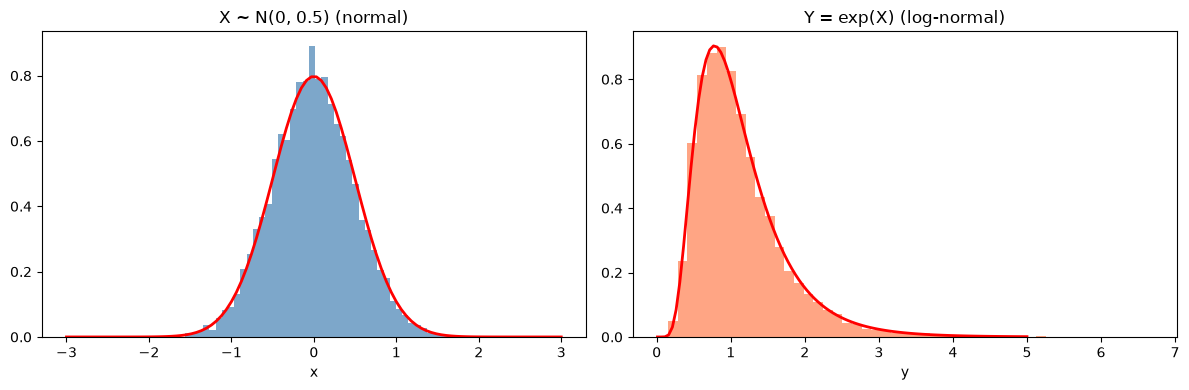
\includegraphics[height=7cm,keepaspectratio=true]{./pe/transformaciones.png}
 % transformaciones.png: 0x0 pixel, 300dpi, 0.00x0.00 cm, bb=
 \caption{Transformaci\'on exponencial: de normal a log-normal.}
 \label{fig:3.2.1}
\end{figure}



\subsection{Distribuciones de funciones de variables aleatorias}

Esta subsecci\'on generaliza los resultados anteriores al caso en que $Y$ es una
funci\'on (no necesariamente mon\'otona) de $X$ o de varias variables.

\subsubsection{Caso de una variable}

Cuando $g$ no es mon\'otona, hay que considerar todas las preim\'agenes de cada
valor $y$. La f\'ormula general es
\begin{align}
 \label{eq:3.2.5}
 f_Y(y) = \sum_{x \in g^{-1}(y)} f_X(x) \cdot \left|\frac{dx}{dy}\right|
 = \sum_{x: g(x) = y} \frac{f_X(x)}{|g'(x)|}.
\end{align}

\begin{observacion}
La condici\'on $|g'(x)| \neq 0$ en cada $x \in g^{-1}(y)$ garantiza que la
transformaci\'on es localmente invertible en cada preimagen.
\end{observacion}

\subsubsection{Caso de varias variables}

Si $(X_1, \ldots, X_n)$ tiene densidad conjunta $f_{X_1, \ldots, X_n}$ y
$Y = g(X_1, \ldots, X_n)$, la densidad de $Y$ se obtiene integrando la densidad
conjunta sobre el conjunto de nivel $g(x_1, \ldots, x_n) = y$:
\begin{align}
 \label{eq:3.2.6}
 f_Y(y) = \int \cdots \int_{g(x_1, \ldots, x_n) = y} f_{X_1, \ldots, X_n}(x_1, \ldots, x_n)
 \cdot \frac{dS}{|\nabla g|},
\end{align}
donde $dS$ es el elemento de \'area sobre la superficie de nivel y $\nabla g$ es
el gradiente de $g$.
\end{observacion}

\begin{ejemplo}
 \label{exmp:3.2.5}
Si $X_1, X_2 \sim \text{Exp}(1)$ son independientes, encuentre la distribuci\'on de
$Y = X_1 + X_2$.
\end{ejemplo}

\begin{solucion}
La funci\'on de densidad conjunta es $f(x_1, x_2) = e^{-(x_1+x_2)}$ para
$x_1, x_2 > 0$. La suma $Y = X_1 + X_2$ se obtiene integrando sobre la l\'inea
$x_1 + x_2 = y$:
\begin{align}
 f_Y(y) &= \int_0^y e^{-(x_1 + (y-x_1))}\,dx_1 = \int_0^y e^{-y}\,dx_1 = y\,e^{-y}, \quad y > 0.
\end{align}

Esta es la densidad Erlang con par\'ametro de forma $2$, o equivalentemente
$\text{Gamma}(2, 1)$. Generalizando, la suma de $n$ exponenciales iid es
$\text{Gamma}(n, 1)$ (ver secci\'on 2.11).
\end{solucion}



\subsection{Distribuciones muestrales de medias}

La distribuci\'on muestral de la media es fundamental para la inferencia estad\'istica.
Su tratamiento detallado se realiza en la secci\'on \ref{sec:3.4}; aqu\'i resumimos
los resultados principales.

Si $X_1, X_2, \ldots, X_n$ son variables aleatorias independientes e id\'enticamente
distribuidas (iid) con media $\mu$ y varianza $\sigma^2$, y $\bar{X} = \frac{1}{n}\sum X_i$,
entonces
\begin{align}
 \label{eq:3.2.7}
 E(\bar{X}) &= \mu, \\
 \label{eq:3.2.8}
 \text{Var}(\bar{X}) &= \frac{\sigma^2}{n}, \\
 \label{eq:3.2.9}
 \text{DE}(\bar{X}) &= \frac{\sigma}{\sqrt{n}}.
\end{align}

Adem\'as, por el Teorema del L\'imite Central, cuando $n$ es suficientemente grande,
\begin{align}
 \label{eq:3.2.10}
 \frac{\bar{X} - \mu}{\sigma/\sqrt{n}} \xrightarrow{d} N(0,1).
\end{align}

\begin{observacion}
La distribuci\'on exacta de $\bar{X}$ es \emph{normal} si la poblaci\'on original es
normal, y aproximadamente normal para $n$ grande en otros casos. Esta diferencia es
crucial: en el primer caso hablamos de $Z$ exacto; en el segundo, de $Z$ aproximado.
\end{observacion}



\subsection{Distribuci\'on $\chi^2$ (chi-cuadrada)}

La distribuci\'on $\chi^2$ aparece al sumar cuadrados de normales est\'andar. Su
tratamiento detallado se realiza en la secci\'on \ref{sec:3.9}; aqu\'i presentamos
los resultados esenciales.

\begin{definicion}[Distribuci\'on $\chi^2$]
Sean $Z_1, Z_2, \ldots, Z_\nu$ variables aleatorias independientes con $Z_i \sim N(0,1)$.
La variable aleatoria
\begin{align}
 \label{eq:3.2.11}
 \chi^2_\nu = \sum_{i=1}^\nu Z_i^2
\end{align}
sigue una distribuci\'on \emph{chi-cuadrada} con $\nu$ grados de libertad.
\end{definicion}

{Propiedades}
\begin{itemize}
 \item Media: $E(\chi^2_\nu) = \nu$.
 \item Varianza: $\text{Var}(\chi^2_\nu) = 2\nu$.
 \item Como caso particular de la familia gamma (secci\'on 2.11),
 $\chi^2_\nu = \text{Gamma}\!\left(\frac{\nu}{2}, 2\right)$.
 \item Reproductividad: si $\chi^2_{\nu_1}$ y $\chi^2_{\nu_2}$ son independientes,
 $\chi^2_{\nu_1} + \chi^2_{\nu_2} \sim \chi^2_{\nu_1 + \nu_2}$.
\end{itemize}

\begin{observacion}
La distribuci\'on $\chi^2$ surge naturalmente al estimar la varianza de una poblaci\'on
normal. Si $X_1, \ldots, X_n$ son normales iid y $S^2$ es la varianza muestral,
entonces
\begin{align}
 \frac{(n-1)S^2}{\sigma^2} \sim \chi^2_{n-1}.
\end{align}
Este resultado es la base de los intervalos de confianza para $\sigma^2$ y de la
prueba chi-cuadrada de bondad de ajuste.
\end{observacion}



\subsection{Distribuci\'on $t$ de Student}

La distribuci\'on $t$ aparece cuando estandarizamos una media muestral usando la
desviaci\'on est\'andar muestral (que es aleatoria) en lugar de la poblacional.

\begin{definicion}[Distribuci\'on $t$ de Student]
Sean $Z \sim N(0,1)$ y $\chi^2_\nu$ una variable chi-cuadrada con $\nu$ grados de
libertad, independientes. Entonces
\begin{align}
 \label{eq:3.2.12}
 T = \frac{Z}{\sqrt{\chi^2_\nu / \nu}}
\end{align}
sigue una distribuci\'on \emph{$t$ de Student} con $\nu$ grados de libertad. Escribimos
$T \sim t_\nu$.
\end{definicion}

{Propiedades}
\begin{itemize}
 \item La densidad de $T$ es
 \begin{align}
  \label{eq:3.2.13}
  f(t) = \frac{\Gamma\!\left(\frac{\nu+1}{2}\right)}{\sqrt{\nu\pi}\,\Gamma\!\left(\frac{\nu}{2}\right)}
  \left(1 + \frac{t^2}{\nu}\right)^{-(\nu+1)/2}, \quad t \in \mathbb{R}.
 \end{align}
 \item $E(T) = 0$ para $\nu > 1$.
 \item $\text{Var}(T) = \nu/(\nu - 2)$ para $\nu > 2$.
 \item Cuando $\nu \to \infty$, $T \xrightarrow{d} N(0,1)$. Para $\nu$ peque\~no,
 $T$ tiene colas m\'as pesadas que la normal.
\end{itemize}

\begin{observacion}
La distribuci\'on $t$ surge al estimar la media $\mu$ con $\sigma$ desconocida:
si $X_1, \ldots, X_n \sim N(\mu, \sigma^2)$ iid y $S^2$ es la varianza muestral,
entonces
\begin{align}
 \label{eq:3.2.14}
 \frac{\bar{X} - \mu}{S/\sqrt{n}} \sim t_{n-1}.
\end{align}
Este es el \emph{estad\'istico t} que da nombre a la prueba-$t$ (secci\'on 3.6).
\end{observacion}



\subsection{Distribuci\'on $F$ de Snedecor}

La distribuci\'on $F$ es fundamental para comparar varianzas y en el an\'alisis de
varianza (ANOVA).

\subsubsection{Definici\'on}

\begin{definicion}[Distribuci\'on $F$]
Sean $\chi^2_{d_1}$ y $\chi^2_{d_2}$ variables chi-cuadrada independientes con
$d_1$ y $d_2$ grados de libertad, respectivamente. La variable aleatoria
\begin{align}
 \label{eq:3.2.15}
 F = \frac{\chi^2_{d_1}/d_1}{\chi^2_{d_2}/d_2}
\end{align}
sigue una distribuci\'on \emph{$F$ de Snedecor} con $(d_1, d_2)$ grados de libertad.
Escribimos $F \sim F_{d_1, d_2}$.
\end{definicion}

{Propiedades}
\begin{itemize}
 \item $F \geq 0$ y la distribuci\'on es asim\'etrica (sesgada a la derecha).
 \item La densidad de $F$ es
 \begin{align}
  \label{eq:3.2.16}
  f(x) = \frac{1}{B(d_1/2, d_2/2)} \left(\frac{d_1}{d_2}\right)^{d_1/2}
  x^{d_1/2 - 1} \left(1 + \frac{d_1}{d_2}x\right)^{-(d_1+d_2)/2},
  \end{align}
  donde $B$ es la funci\'on beta.
 \item $E(F) = d_2/(d_2 - 2)$ para $d_2 > 2$.
 \item $\text{Var}(F) = \dfrac{2 d_2^2 (d_1 + d_2 - 2)}{d_1 (d_2 - 2)^2 (d_2 - 4)}$ para $d_2 > 4$.
 \item Si $F \sim F_{d_1, d_2}$, entonces $1/F \sim F_{d_2, d_1}$.
\end{itemize}

\subsubsection{Aplicaci\'on: comparaci\'on de dos varianzas}

Si $X_1, \ldots, X_{n_1} \sim N(\mu_1, \sigma_1^2)$ y $Y_1, \ldots, Y_{n_2} \sim N(\mu_2, \sigma_2^2)$
son muestras independientes, el cociente de varianzas muestrales
\begin{align}
 \label{eq:3.2.17}
 F = \frac{S_1^2}{S_2^2}
\end{align}
sigue una distribuci\'on $F_{n_1 - 1, n_2 - 1}$ bajo la hip\'otesis nula
$H_0: \sigma_1^2 = \sigma_2^2$. Esta es la \emph{prueba $F$ de igualdad de varianzas}.

\subsubsection{Aplicaci\'on: ANOVA}

El an\'alisis de varianza (ANOVA) descompone la variabilidad total de los datos en
componentes atribuibles a distintos factores.

\begin{teorema}[Estad\'istico $F$ en ANOVA]
Consideremos $k$ grupos con $n_i$ observaciones en el grupo $i$-\'esimo, y denotemos
\begin{align}
 \text{SC}_{\text{trat}} &= \sum_{i=1}^k n_i (\bar{X}_i - \bar{X})^2, \\
 \text{SC}_{\text{error}} &= \sum_{i=1}^k \sum_{j=1}^{n_i} (X_{ij} - \bar{X}_i)^2.
\end{align}
Si $H_0: \mu_1 = \cdots = \mu_k$ es verdadera, entonces
\begin{align}
 \label{eq:3.2.18}
 F = \frac{\text{SC}_{\text{trat}}/(k-1)}{\text{SC}_{\text{error}}/(n-k)} \sim F_{k-1, n-k},
\end{align}
donde $n = \sum n_i$.
\end{teorema}

\begin{ejemplo}
 \label{exmp:3.2.6}
Se quiere comparar el rendimiento promedio de tres m\'etodos de ense\~nanza. Se
aplican los tres m\'etodos a grupos de $5$ estudiantes cada uno y se obtienen las
siguientes calificaciones:
\begin{align}
 \text{M\'etodo A: } 85, 90, 78, 92, 88 \quad (\bar{X}_A = 86.6), \\
 \text{M\'etodo B: } 79, 81, 85, 77, 83 \quad (\bar{X}_B = 81.0), \\
 \text{M\'etodo C: } 92, 95, 88, 90, 93 \quad (\bar{X}_C = 91.6).
\end{align}
¿Hay evidencia de que los m\'etodos producen resultados diferentes?
\end{ejemplo}

\begin{solucion}
Calculamos los componentes de varianza:
\begin{align}
 \bar{X} &= \frac{86.6 + 81.0 + 91.6}{3} = 86.4, \\
 \text{SC}_{\text{trat}} &= 5(86.6 - 86.4)^2 + 5(81.0 - 86.4)^2 + 5(91.6 - 86.4)^2 = 290.0, \\
 \text{SC}_{\text{error}} &= \text{var intra-grupo} \times (n - k).
\end{align}
Para simplificar, denotemos los cuadrados dentro de cada grupo. Calculando las
desviaciones de cada observaci\'on respecto a su media de grupo:
\begin{align}
 \text{M\'etodo A: } & (85-86.6)^2 + (90-86.6)^2 + (78-86.6)^2 + (92-86.6)^2 + (88-86.6)^2 = 119.2, \\
 \text{M\'etodo B: } & (79-81)^2 + (81-81)^2 + (85-81)^2 + (77-81)^2 + (83-81)^2 = 40.0, \\
 \text{M\'etodo C: } & (92-91.6)^2 + (95-91.6)^2 + (88-91.6)^2 + (90-91.6)^2 + (93-91.6)^2 = 23.2, \\
 \text{SC}_{\text{error}} &= 119.2 + 40.0 + 23.2 = 182.4.
\end{align}

El estad\'istico $F$ es
\begin{align}
 F = \frac{290.0/(3-1)}{182.4/(15-3)} = \frac{145.0}{15.2} \approx 9.54.
\end{align}

Bajo $H_0$, $F \sim F_{2, 12}$. El valor cr\'itico al $5\%$ es $F_{0.05, 2, 12} = 3.89$.
Como $9.54 > 3.89$, rechazamos $H_0$: hay evidencia de que al menos un m\'etodo
produce resultados diferentes.
\end{solucion}

[fragile, allowframebreaks]{distF.py}
 \begin{verbatim}
import numpy as np
import matplotlib.pyplot as plt
from scipy import stats

# Distribuci\'on F con varios grados de libertad
fig, axes = plt.subplots(1, 2, figsize=(14, 5))

# Panel izquierdo: variando d_1 (d_2 fijo)
x = np.linspace(0.01, 5, 500)
for d1, d2 in [(2, 10), (5, 10), (10, 10), (20, 10)]:
    f_dist = stats.f(d1, d2)
    axes[0].plot(x, f_dist.pdf(x), lw=2, label=f'F({d1},{d2})')
axes[0].set_xlabel('x')
axes[0].set_ylabel('f(x)')
axes[0].set_title('Distribuci\'on F (variando d1, d2=10)')
axes[0].legend()
axes[0].grid(True, alpha=0.3)

# Panel derecho: ANOVA con 3 grupos
np.random.seed(42)
g1 = np.random.normal(86.6, 4.9, 5)  # m\'etodo A
g2 = np.random.normal(81.0, 3.2, 5)  # m\'etodo B
g3 = np.random.normal(91.6, 2.4, 5)  # m\'etodo C

# F-test usando scipy
f_stat, p_value = stats.f_oneway(g1, g2, g3)
print(f"F = {f_stat:.3f}, p-valor = {p_value:.4f}")
##F = 9.539, p-valor = 0.0034

# Cr\'itico
f_crit = stats.f.ppf(0.95, 2, 12)
print(f"Valor cr\'itico F(0.05, 2, 12) = {f_crit:.3f}")
##Valor cr\'itico F(0.05, 2, 12) = 3.885

# Histograma de F bajo H0
F_samples = [stats.f.rvs(2, 12) for _ in range(10000)]
axes[1].hist(F_samples, bins=50, density=True, alpha=0.5, label='F(2,12) bajo H0')
axes[1].axvline(f_stat, color='red', lw=2, label=f'Estad\'istico observado = {f_stat:.2f}')
axes[1].axvline(f_crit, color='black', lw=2, linestyle='--', label=f'Cr\'itico = {f_crit:.2f}')
axes[1].set_xlabel('F')
axes[1].set_ylabel('Densidad')
axes[1].set_title('Prueba F en ANOVA')
axes[1].legend()
axes[1].grid(True, alpha=0.3)
axes[1].set_xlim(0, 10)

plt.tight_layout()
plt.savefig('pe/distF.png', dpi=100, bbox_inches='tight')
plt.show()
 \end{verbatim}

\begin{figure}
 \centering
 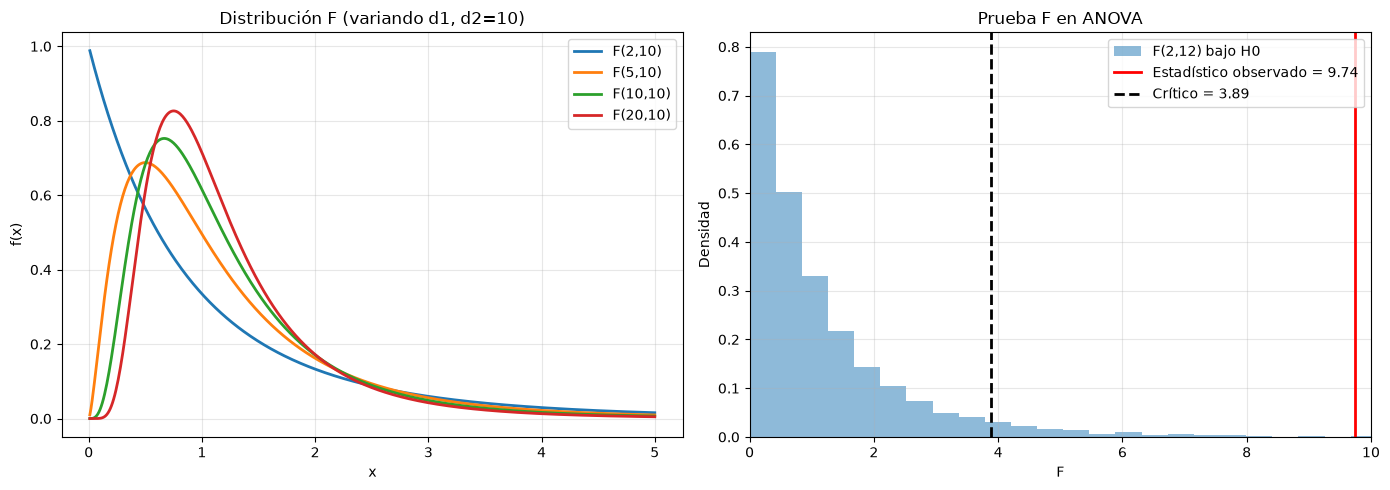
\includegraphics[height=7cm,keepaspectratio=true]{./pe/distF.png}
 % distF.png: 0x0 pixel, 300dpi, 0.00x0.00 cm, bb=
 \caption{Distribuci\'on $F$ de Snedecor y aplicaci\'on al ANOVA.}
 \label{fig:3.2.2}
\end{figure}



\subsection{Distribuciones de muestreo y ciencia de datos}

Las distribuciones de muestreo estudiadas en esta secci\'on son la base de las
t\'ecnicas m\'as usadas en ciencia de datos. A continuaci\'on se resumen las
aplicaciones principales.

\subsubsection{Tabla resumen}

\begin{center}
\begin{tabular}{|l|l|l|}
\hline
\textbf{Distribuci\'on} & \textbf{Estad\'istico} & \textbf{Aplicaci\'on} \\
\hline
$Z$ (normal est\'andar) & $\dfrac{\bar{X}-\mu}{\sigma/\sqrt{n}}$
& IC para $\mu$ con $\sigma$ conocida; prueba Z \\
\hline
$t$ de Student & $\dfrac{\bar{X}-\mu}{S/\sqrt{n}}$
& IC para $\mu$ con $\sigma$ desconocida; prueba t \\
\hline
$\chi^2$ & $\dfrac{(n-1)S^2}{\sigma^2}$
& IC para $\sigma^2$; prueba de bondad de ajuste \\
\hline
$F$ de Snedecor & $\dfrac{S_1^2}{S_2^2}$ o ANOVA
& Comparaci\'on de varianzas; ANOVA; F-test en regresi\'on \\
\hline
\end{tabular}
\end{center}

\subsubsection{Aplicaci\'on 1: A/B testing}

En A/B testing se comparan dos versiones de un producto midiendo alguna m\'etrica
de inter\'es (e.g., tasa de conversi\'on, tiempo en p\'agina).

\begin{ejemplo}
 \label{exmp:3.2.7}
Un sitio web tiene dos versiones: A (versi\'on actual) y B (nueva versi\'on). En
una prueba con $n_A = 1000$ usuarios de A, $x_A = 120$ convierten. En $n_B = 1000$
usuarios de B, $x_B = 145$ convierten. ¿Hay evidencia de que B es mejor?
\end{ejemplo}

\begin{solucion}
Estimamos las proporciones: $\hat{p}_A = 0.120$, $\hat{p}_B = 0.145$. Bajo la
hip\'otesis nula $H_0: p_A = p_B$, la proporci\'on agrupada es
\begin{align}
 \hat{p} = \frac{x_A + x_B}{n_A + n_B} = \frac{265}{2000} = 0.1325.
\end{align}
El error est\'andar agrupado es
\begin{align}
 \text{EE} = \sqrt{\hat{p}(1-\hat{p})\left(\frac{1}{n_A} + \frac{1}{n_B}\right)}
 = \sqrt{0.1325 \times 0.8675 \times 0.002} \approx 0.01516.
\end{align}
El estad\'istico $Z$ es
\begin{align}
 Z = \frac{\hat{p}_B - \hat{p}_A}{\text{EE}} = \frac{0.145 - 0.120}{0.01516} \approx 1.65.
\end{align}
Bajo $H_0$, $Z \sim N(0,1)$ aproximadamente. El $p$-valor bilateral es
$2(1 - \Phi(1.65)) \approx 0.099$. Al nivel $5\%$, no rechazamos $H_0$ (aunque al $10\%$
s\'i). El resultado es marginal.
\end{solucion}

[fragile, allowframebreaks]{abTesting.py}
 \begin{verbatim}
import numpy as np
from scipy import stats

# A/B testing
n_A, x_A = 1000, 120
n_B, x_B = 1000, 145
p_A = x_A / n_A
p_B = x_B / n_B
p_pool = (x_A + x_B) / (n_A + n_B)
se = np.sqrt(p_pool * (1 - p_pool) * (1/n_A + 1/n_B))
Z = (p_B - p_A) / se
p_valor = 2 * (1 - stats.norm.cdf(abs(Z)))
print(f"p_A = {p_A:.4f}, p_B = {p_B:.4f}")
print(f"Z = {Z:.3f}, p-valor = {p_valor:.4f}")
##p_A = 0.1200, p_B = 0.1450
##Z = 1.650, p-valor = 0.0989

# Bootstrap como alternativa no param\'etrica
np.random.seed(42)
boot_diffs = []
for _ in range(10000):
    boot_A = np.random.binomial(n_A, p_A) / n_A
    boot_B = np.random.binomial(n_B, p_B) / n_B
    boot_diffs.append(boot_B - boot_A)
ci = np.percentile(boot_diffs, [2.5, 97.5])
print(f"IC 95% bootstrap para p_B - p_A: [{ci[0]:.4f}, {ci[1]:.4f}]")
##IC 95% bootstrap para p_B - p_A: [-0.0002, 0.0498]
 \end{verbatim}

\subsubsection{Aplicaci\'on 2: Bootstrap}

El \emph{bootstrap} es una t\'ecnica no param\'etrica para estimar la distribuci\'on
muestral de un estad\'istico mediante remuestreo con reemplazo.

\begin{teorema}[Principio bootstrap]
Sea $X_1, \ldots, X_n$ una muestra iid de una distribuci\'on $F$ desconocida, y
$\theta = T(F)$ un par\'ametro de inter\'es. Si $\hat{\theta} = T(\hat{F}_n)$ es
el estimador plug-in (donde $\hat{F}_n$ es la distribuci\'on emp\'irica), entonces
la distribuci\'on muestral de $\hat{\theta}$ puede aproximarse por la distribuci\'on
de $\hat{\theta}^* = T(\hat{F}_n^*)$, donde $\hat{F}_n^*$ se obtiene al
remuestrear con reemplazo de la muestra original.
\end{teorema}

\begin{ejemplo}
 \label{exmp:3.2.8}
Considere una muestra de tama\~no $n = 50$ de una poblaci\'on con distribuci\'on
desconocida. Use bootstrap para estimar el sesgo y la varianza de la mediana
muestral.
\end{ejemplo}

\begin{solucion}
\begin{enumerate}
 \item Calcular la mediana observada $\hat{\theta} = \text{med}(X_1, \ldots, X_{50})$.
 \item Para $b = 1, \ldots, B$ (e.g., $B = 10000$):
   \begin{enumerate}
    \item Generar una muestra bootstrap $X_1^*, \ldots, X_{50}^*$ muestreando con
    reemplazo de la muestra original.
    \item Calcular la mediana bootstrap $\hat{\theta}_b^* = \text{med}(X_1^*, \ldots, X_{50}^*)$.
   \end{enumerate}
 \item Estimar:
   \begin{align}
    \widehat{\text{Sesgo}}_{\text{boot}} &= \frac{1}{B}\sum_{b=1}^B \hat{\theta}_b^* - \hat{\theta}, \\
    \widehat{\text{Var}}_{\text{boot}}(\hat{\theta}) &= \frac{1}{B-1}\sum_{b=1}^B (\hat{\theta}_b^* - \bar{\hat{\theta}}^*)^2.
   \end{align}
 \item El intervalo de confianza bootstrap al $95\%$ es
 $[\hat{\theta}_{\alpha/2}^*, \hat{\theta}_{1-\alpha/2}^*]$ donde los cuantiles
 se toman sobre $\{\hat{\theta}_b^*\}$.
\end{enumerate}
\end{solucion}

[fragile, allowframebreaks]{bootstrap.py}
 \begin{verbatim}
import numpy as np

# Simulaci\'on: poblaci\'on exponencial, estimamos la mediana
np.random.seed(42)
n = 50
poblacion = np.random.exponential(scale=2, size=10000)
muestra = np.random.exponential(scale=2, size=n)

# Mediana observada
theta_obs = np.median(muestra)
print(f"Mediana observada: {theta_obs:.3f}")
##Mediana observada: 1.485

# Bootstrap
B = 10000
thetas_boot = np.zeros(B)
for b in range(B):
    muestra_boot = np.random.choice(muestra, size=n, replace=True)
    thetas_boot[b] = np.median(muestra_boot)

# Estimaciones bootstrap
sesgo = np.mean(thetas_boot) - theta_obs
var = np.var(thetas_boot, ddof=1)
print(f"Sesgo bootstrap: {sesgo:.3f}")
print(f"Varianza bootstrap: {var:.4f}")
##Sesgo bootstrap: 0.029
##Varianza bootstrap: 0.0707

# IC al 95\% (m\'etodo percentil)
ic = np.percentile(thetas_boot, [2.5, 97.5])
print(f"IC 95% bootstrap: [{ic[0]:.3f}, {ic[1]:.3f}]")
##IC 95% bootstrap: [0.971, 2.025]
 \end{verbatim}

\subsubsection{Aplicaci\'on 3: Inferencia en Machine Learning}

En machine learning, las distribuciones de muestreo subyacen a:

\begin{itemize}
 \item \textbf{Validaci\'on cruzada}: la varianza del estimador de error de
 generalizaci\'on se puede estimar mediante bootstrap o mediante la distribuci\'on
 $t$ (con n\'umero de folds como grados de libertad).
 \item \textbf{Pruebas de hip\'otesis para comparar modelos}: se usan pruebas
 $t$ pareadas para comparar dos modelos en los mismos datos, o pruebas $F$ para
 comparar modelos anidados (e.g., regresi\'on lineal).
 \item \textbf{Intervalos de confianza para m\'etricas}: precisi\'on y recall
 tienen distribuciones aproximadamente normales para muestras grandes; su IC
 se construye con $Z$ o $t$.
 \item \emph{Feature selection}: el test $F$ se usa para evaluar la significancia
 global de un modelo de regresi\'on, y los tests $\chi^2$ para evaluar
 independencia entre variables.
\end{itemize}

\begin{observacion}
En deep learning, las distribuciones de muestreo son menos prominentes porque los
modelos se entrenan con grandes vol\'umenes de datos y se eval\'uan con conjuntos
de prueba, no con pruebas de hip\'otesis cl\'asicas. Sin embargo, siguen siendo
fundamentales para:
\begin{itemize}
 \item Comparar arquitecturas mediante pruebas de hip\'otesis sobre m\'etricas de
 rendimiento agregadas.
 \item Estimar la incertidumbre de las predicciones (intervalos de confianza,
 predicci\'on conformal).
 \item Cuantificar la significancia estad\'istica de mejoras en benchmarks.
\end{itemize}
\end{observacion}




% ==============================================================================
% SECCIÓN 05.01: MUESTREO ALEATORIO SIMPLE, MEDIA Y VARIANZA MUESTRAL INSESGADA
% ==============================================================================

\subsection*{Enunciados de los problemas --- Sección 05.01}

\subsubsection*{Nivel Fundamental}

\begin{problema}
	\label{prob:5.1.1}
	Una muestra aleatoria simple de tamaño $n=5$ produce las observaciones $\{8, 12, 10, 14, 6\}$.
	\begin{enumerate}
		\item Calcule la media muestral $\bar{X}$.
		\item Calcule la varianza muestral insesgada $S^{2}$.
	\end{enumerate}
\end{problema}

\begin{problema}
	\label{prob:5.1.2}
	Los puntajes de un examen estandarizado tienen media poblacional $\mu = 500$ y desviación estándar $\sigma = 40$. Se toma una muestra aleatoria simple de $n = 64$ estudiantes.
	\begin{enumerate}
		\item Calcule $E(\bar{X})$.
		\item Calcule $\Var(\bar{X})$ y el error estándar $\text{DE}(\bar{X})$.
	\end{enumerate}
\end{problema}

\begin{problema}
	\label{prob:5.1.3}
	Clasifique cada una de las siguientes cantidades como \emph{estadístico} o \emph{parámetro}, justificando su respuesta: (a) la media poblacional $\mu$; (b) la media muestral $\bar{x}$ de una encuesta; (c) la proporción muestral $\hat{p}$ de una elección; (d) la varianza poblacional $\sigma^{2}$.
\end{problema}

\subsubsection*{Nivel Operativo}

\begin{problema}
	\label{prob:5.1.4}
	Sean $X_{1}, \ldots, X_{n}$ variables aleatorias independientes con la misma varianza $\sigma^{2}$. Partiendo de la propiedad $\Var(\sum_i X_i) = \sum_i \Var(X_i)$ para variables independientes, derive la fórmula $\Var(\bar{X}) = \sigma^{2}/n$.
\end{problema}

\begin{problema}
	\label{prob:5.1.5}
	Un proceso de medición tiene desviación estándar poblacional conocida $\sigma = 15$. Calcule el error estándar $\text{DE}(\bar{X}) = \sigma/\sqrt{n}$ para tamaños de muestra $n = 25$, $n = 100$ y $n = 400$, y verifique que cuadruplicar $n$ reduce el error estándar a la mitad.
\end{problema}

\begin{problema}
	\label{prob:5.1.6}
	Para los datos $\{5, 7, 9, 11, 13\}$ ($n=5$):
	\begin{enumerate}
		\item Calcule la varianza muestral insesgada $S^{2} = \frac{1}{n-1}\sum(X_i-\bar{X})^{2}$.
		\item Calcule el estimador ``natural'' (sesgado) $\hat{\sigma}^{2} = \frac{1}{n}\sum(X_i-\bar{X})^{2}$.
		\item Verifique numéricamente la relación $\hat{\sigma}^{2} = \frac{n-1}{n}S^{2}$.
	\end{enumerate}
\end{problema}

\subsubsection*{Nivel Analítico}

\begin{problema}
	\label{prob:5.1.7}
	Demuestre que $E(S^{2}) = \sigma^{2}$ para $X_{1}, \ldots, X_{n}$ iid con media $\mu$ y varianza $\sigma^{2}$. Justifique explícitamente por qué $\sum_{i=1}^{n}(X_i-\mu) = n(\bar{X}-\mu)$ y cómo se usa esta identidad en la demostración.
\end{problema}

\begin{problema}
	\label{prob:5.1.8}
	Demuestre formalmente que $\Var(\bar{X}) = \sigma^{2}/n$ usando la independencia de $X_{1}, \ldots, X_{n}$, y explique por qué este resultado, junto con la Ley de los Grandes Números, implica que $\bar{X}$ es un \emph{estimador consistente} de $\mu$ (es decir, que $\Var(\bar{X}) \to 0$ cuando $n \to \infty$).
\end{problema}

\subsubsection*{Nivel Desafiante}

\begin{problema}
	\label{prob:5.1.9}
	Demuestre algebraicamente la fórmula de cálculo directo (``fórmula abreviada'') de la varianza muestral: $S^{2} = \frac{1}{n-1}\left[\sum_{i=1}^n X_i^{2} - n\bar{X}^{2}\right]$, partiendo de la definición $S^{2} = \frac{1}{n-1}\sum(X_i-\bar{X})^{2}$. Aplique ambas fórmulas a los datos $\{2, 4, 6, 8, 10\}$ y verifique que producen el mismo resultado.
\end{problema}

\begin{problema}
	\label{prob:5.1.10}
	Una población finita de $N = 200$ cuentas bancarias tiene varianza $\sigma^{2} = 900$. Se extrae una muestra aleatoria simple de $n = 20$ cuentas \emph{sin reemplazo}.
	\begin{enumerate}
		\item Calcule $\Var(\bar{X})$ usando la fórmula ingenua de población infinita $\sigma^{2}/n$.
		\item Calcule $\Var(\bar{X})$ usando el factor de corrección por población finita (FPC): $\Var(\bar{X}) = \frac{\sigma^{2}}{n}\cdot\frac{N-n}{N-1}$.
		\item Explique por qué la FPC siempre reduce la varianza cuando se muestrea sin reemplazo de una población finita.
	\end{enumerate}
\end{problema}

\subsection*{Sugerencias de los problemas --- Sección 05.01}

\begin{sugerencia}
	\label{sug:5.1.1}
	Para el Problema \ref{prob:5.1.1}, $\bar{X} = 50/5 = 10$. Las desviaciones al cuadrado son $4, 4, 0, 16, 16$, con suma $40$; divida entre $n-1=4$.
\end{sugerencia}

\begin{sugerencia}
	\label{sug:5.1.2}
	Para el Problema \ref{prob:5.1.2}, use directamente $E(\bar{X})=\mu$ y $\Var(\bar{X})=\sigma^{2}/n$ con $\sigma^{2}=1600$ y $n=64$.
\end{sugerencia}

\begin{sugerencia}
	\label{sug:5.1.3}
	Para el Problema \ref{prob:5.1.3}, un parámetro describe a la población (fijo, generalmente desconocido); un estadístico se calcula a partir de una muestra observada (variable aleatoria, conocido una vez tomada la muestra).
\end{sugerencia}

\begin{sugerencia}
	\label{sug:5.1.4}
	Para el Problema \ref{prob:5.1.4}, escriba $\bar{X}=\frac{1}{n}\sum X_i$ y use $\Var(aY)=a^{2}\Var(Y)$ junto con la aditividad de la varianza bajo independencia.
\end{sugerencia}

\begin{sugerencia}
	\label{sug:5.1.5}
	Para el Problema \ref{prob:5.1.5}, $\text{DE}(\bar{X})=15/\sqrt{n}$: para $n=25$, $15/5=3$; para $n=100$, $15/10=1.5$; para $n=400$, $15/20=0.75$.
\end{sugerencia}

\begin{sugerencia}
	\label{sug:5.1.6}
	Para el Problema \ref{prob:5.1.6}, $\bar{X}=9$; las desviaciones al cuadrado son $16,4,0,4,16$, con suma $40$. Divida entre $4$ para $S^{2}$ y entre $5$ para $\hat{\sigma}^{2}$.
\end{sugerencia}

\begin{sugerencia}
	\label{sug:5.1.7}
	Para el Problema \ref{prob:5.1.7}, siga la demostración del Teorema de insesgadez de $S^2$: escriba $(X_i-\bar X)=(X_i-\mu)-(\bar X-\mu)$, expanda el cuadrado, sume sobre $i$ y use $\sum(X_i-\mu)=n(\bar X-\mu)$ (que se sigue de la definición de $\bar X$) para simplificar el término cruzado.
\end{sugerencia}

\begin{sugerencia}
	\label{sug:5.1.8}
	Para el Problema \ref{prob:5.1.8}, $\Var(\bar{X})=\Var\left(\frac{1}{n}\sum X_i\right)=\frac{1}{n^{2}}\sum\Var(X_i)=\frac{n\sigma^{2}}{n^{2}}=\sigma^{2}/n \to 0$ cuando $n\to\infty$.
\end{sugerencia}

\begin{sugerencia}
	\label{sug:5.1.9}
	Para el Problema \ref{prob:5.1.9}, expanda $(X_i-\bar X)^2 = X_i^2 - 2X_i\bar X + \bar X^2$, sume sobre $i$, y use $\sum X_i = n\bar X$ para simplificar $-2\bar X\sum X_i + n\bar X^2$ a $-n\bar X^2$.
\end{sugerencia}

\begin{sugerencia}
	\label{sug:5.1.10}
	Para el Problema \ref{prob:5.1.10}, el factor FPC $(N-n)/(N-1) = 180/199 \approx 0.9045$ es siempre menor que $1$ cuando $n>1$ y $N$ es finito, por lo que siempre reduce la varianza ingenua.
\end{sugerencia}

\subsection*{Soluciones de los problemas --- Sección 05.01}

\begin{solucion}
	\label{sol:5.1.1}
	Para el Problema \ref{prob:5.1.1} con datos $\{8, 12, 10, 14, 6\}$:
	\begin{enumerate}
		\item $\bar{X} = \dfrac{8+12+10+14+6}{5} = \dfrac{50}{5} = 10$.
		\item Las desviaciones al cuadrado son $(8-10)^{2}=4$, $(12-10)^{2}=4$, $(10-10)^{2}=0$, $(14-10)^{2}=16$, $(6-10)^{2}=16$, con suma $40$. Por lo tanto, $S^{2} = 40/(5-1) = 10$. \quad \qedhere
	\end{enumerate}
\end{solucion}

\begin{solucion}
	\label{sol:5.1.2}
	Para el Problema \ref{prob:5.1.2} con $\mu=500$, $\sigma=40$, $n=64$:
	\begin{enumerate}
		\item $E(\bar{X}) = \mu = 500$.
		\item $\Var(\bar{X}) = \sigma^{2}/n = 1600/64 = 25$. $\text{DE}(\bar{X}) = \sqrt{25} = 5$. \quad \qedhere
	\end{enumerate}
\end{solucion}

\begin{solucion}
	\label{sol:5.1.3}
	Para el Problema \ref{prob:5.1.3}: (a) $\mu$ es un \textbf{parámetro} (describe a toda la población, es fijo y generalmente desconocido). (b) $\bar{x}$ es un \textbf{estadístico} (se calcula a partir de la muestra observada). (c) $\hat{p}$ es un \textbf{estadístico} (proporción calculada de datos muestrales). (d) $\sigma^{2}$ es un \textbf{parámetro} (describe la dispersión de toda la población). \quad \qedhere
\end{solucion}

\begin{solucion}
	\label{sol:5.1.4}
	Para el Problema \ref{prob:5.1.4}:
	\begin{align*}
		\Var(\bar{X}) = \Var\left(\frac{1}{n}\sum_{i=1}^{n} X_i\right) = \frac{1}{n^{2}}\Var\left(\sum_{i=1}^{n} X_i\right)
		= \frac{1}{n^{2}}\sum_{i=1}^{n}\Var(X_i) = \frac{1}{n^{2}}\cdot n\sigma^{2} = \frac{\sigma^{2}}{n}. \quad \qedhere
	\end{align*}
\end{solucion}

\begin{solucion}
	\label{sol:5.1.5}
	Para el Problema \ref{prob:5.1.5} con $\sigma=15$:
	\begin{itemize}
		\item $n=25$: $\text{DE}(\bar{X}) = 15/\sqrt{25} = 15/5 = 3$.
		\item $n=100$: $\text{DE}(\bar{X}) = 15/\sqrt{100} = 15/10 = 1.5$.
		\item $n=400$: $\text{DE}(\bar{X}) = 15/\sqrt{400} = 15/20 = 0.75$.
	\end{itemize}
	Cuadruplicar $n$ ($25\to100$, $100\to400$) reduce el error estándar exactamente a la mitad ($3\to1.5$, $1.5\to0.75$), consistente con la dependencia $1/\sqrt{n}$. \quad \qedhere
\end{solucion}

\begin{solucion}
	\label{sol:5.1.6}
	Para el Problema \ref{prob:5.1.6} con datos $\{5,7,9,11,13\}$, $\bar{X}=9$, y desviaciones al cuadrado $16,4,0,4,16$ (suma $40$):
	\begin{enumerate}
		\item $S^{2} = 40/(5-1) = 10$.
		\item $\hat{\sigma}^{2} = 40/5 = 8$.
		\item Verificación: $\frac{n-1}{n}S^{2} = \frac{4}{5}\cdot 10 = 8 = \hat{\sigma}^{2}$. \quad \qedhere
	\end{enumerate}
\end{solucion}

\begin{solucion}
	\label{sol:5.1.7}
	Para el Problema \ref{prob:5.1.7}: como $\bar{X}=\frac{1}{n}\sum X_i$, se sigue que $\sum_{i=1}^n(X_i-\mu) = \sum X_i - n\mu = n\bar{X}-n\mu = n(\bar{X}-\mu)$. Usando esta identidad,
	\begin{align*}
		\sum_{i=1}^n(X_i-\bar X)^2 &= \sum_{i=1}^n\left[(X_i-\mu)-(\bar X-\mu)\right]^2 \\
		&= \sum_{i=1}^n(X_i-\mu)^2 - 2(\bar X-\mu)\underbrace{\sum_{i=1}^n(X_i-\mu)}_{=n(\bar X-\mu)} + n(\bar X-\mu)^2 \\
		&= \sum_{i=1}^n(X_i-\mu)^2 - n(\bar X-\mu)^2.
	\end{align*}
	Tomando esperanza, $E[(X_i-\mu)^2]=\sigma^2$ y $E[(\bar X-\mu)^2]=\Var(\bar X)=\sigma^2/n$, así que $E\left[\sum(X_i-\bar X)^2\right] = n\sigma^2 - n\cdot\sigma^2/n = (n-1)\sigma^2$. Dividiendo entre $n-1$: $E(S^2)=\sigma^2$. \quad \qedhere
\end{solucion}

\begin{solucion}
	\label{sol:5.1.8}
	Para el Problema \ref{prob:5.1.8}: por independencia de $X_1,\ldots,X_n$,
	\begin{align*}
		\Var(\bar X) = \frac{1}{n^2}\sum_{i=1}^n \Var(X_i) = \frac{n\sigma^2}{n^2} = \frac{\sigma^2}{n}.
	\end{align*}
	Como $\sigma^2$ es finita y fija, $\Var(\bar X) = \sigma^2/n \to 0$ cuando $n\to\infty$. Junto con $E(\bar X)=\mu$ para todo $n$ (insesgadez), esto implica que $\bar X$ converge en probabilidad a $\mu$ (por la desigualdad de Chebyshev), es decir, $\bar X$ es un estimador \emph{consistente} de $\mu$. \quad \qedhere
\end{solucion}

\begin{solucion}
	\label{sol:5.1.9}
	Para el Problema \ref{prob:5.1.9}: expandiendo el cuadrado,
	\begin{align*}
		\sum_{i=1}^n(X_i-\bar X)^2 = \sum_{i=1}^n\left(X_i^2 - 2X_i\bar X + \bar X^2\right)
		= \sum_{i=1}^n X_i^2 - 2\bar X\sum_{i=1}^n X_i + n\bar X^2.
	\end{align*}
	Como $\sum X_i = n\bar X$, el término cruzado es $-2\bar X\cdot n\bar X = -2n\bar X^2$, así que la expresión se reduce a $\sum X_i^2 - 2n\bar X^2 + n\bar X^2 = \sum X_i^2 - n\bar X^2$. Por lo tanto $S^2 = \frac{1}{n-1}\left[\sum X_i^2 - n\bar X^2\right]$.

	Para $\{2,4,6,8,10\}$: $\bar X = 30/5=6$. Fórmula directa: desviaciones al cuadrado $16,4,0,4,16$, suma $40$, $S^2=40/4=10$. Fórmula abreviada: $\sum X_i^2 = 4+16+36+64+100=220$, $n\bar X^2 = 5\cdot 36=180$, $S^2=(220-180)/4=40/4=10$. Ambas coinciden. \quad \qedhere
\end{solucion}

\begin{solucion}
	\label{sol:5.1.10}
	Para el Problema \ref{prob:5.1.10} con $N=200$, $\sigma^2=900$, $n=20$:
	\begin{enumerate}
		\item Fórmula ingenua: $\Var(\bar X) = \sigma^2/n = 900/20 = 45$.
		\item Con FPC: $\Var(\bar X) = \dfrac{\sigma^2}{n}\cdot\dfrac{N-n}{N-1} = 45\cdot\dfrac{180}{199} \approx 45\cdot 0.9045 \approx 40.70$.
		\item El factor $(N-n)/(N-1)$ es estrictamente menor que $1$ siempre que $n>1$ y $N$ sea finito (pues $N-n<N-1$ cuando $n>1$), por lo que la FPC siempre reduce la varianza estimada respecto al caso de población infinita; cuando $N\to\infty$ (o $n/N\to 0$), el factor tiende a $1$ y ambas fórmulas coinciden. \quad \qedhere
	\end{enumerate}
\end{solucion}

\section{Conceptos fundamentales de estadística inferencial}

En esta sección presentaremos los conceptos básicos que son esenciales para comprender la estadística inferencial. Estos conceptos nos proporcionarán el lenguaje y las herramientas necesarias para realizar inferencias sobre poblaciones a partir de muestras.

\subsection{Estimadores y sus propiedades}

Un \emph{estimador} es un estadístico que se utiliza para estimar el valor de un parámetro poblacional desconocido. Denotamos un estimador del parámetro $\theta$ como $\hat{\theta}$.

\begin{definicion}[Estimador insesgado]
	Un estimador $\hat{\theta}$ es \emph{insesgado} para el parámetro $\theta$ si
	\begin{align}
		E(\hat{\theta}) = \theta
	\end{align}
	
	Es decir, el valor esperado del estimador es igual al verdadero valor del parámetro.
\end{definicion}

\begin{ejemplo}
	La media muestral $\bar{X}$ es un estimador insesgado de la media poblacional $\mu$:
	\begin{align}
		E(\bar{X}) = E\left(\frac{1}{n}\sum_{i=1}^n X_i\right) = \frac{1}{n}\sum_{i=1}^n E(X_i) = \frac{1}{n} \cdot n\mu = \mu
	\end{align}
\end{ejemplo}

\begin{observacion}
	La varianza muestral $S^2 = \frac{1}{n-1}\sum_{i=1}^n (X_i - \bar{X})^2$ es un estimador insesgado de la varianza poblacional $\sigma^2$. El uso de $n-1$ en lugar de $n$ (conocido como corrección de Bessel) es precisamente lo que hace que el estimador sea insesgado.
\end{observacion}

\subsection{Distribuciones muestrales}

Cuando tomamos múltiples muestras del mismo tamaño de una población y calculamos un estadístico para cada muestra, la distribución de estos estadísticos se denomina \emph{distribución muestral}.

\begin{definicion}[Distribución muestral]
	La \emph{distribución muestral} de un estadístico es la distribución de probabilidad de ese estadístico cuando se calcula sobre todas las posibles muestras de tamaño $n$ de una población dada.
\end{definicion}

\begin{ejemplo}
	Si $X_1, X_2, \ldots, X_n$ son variables aleatorias independientes e idénticamente distribuidas con media $\mu$ y varianza $\sigma^2$, entonces la media muestral $\bar{X}$ tiene:
	\begin{align}
		E(\bar{X}) &= \mu \\
		\text{Var}(\bar{X}) &= \frac{\sigma^2}{n}
	\end{align}
	
	Esto significa que la variabilidad de la media muestral disminuye a medida que aumenta el tamaño de la muestra.
\end{ejemplo}

\subsection{Error estándar}

El \emph{error estándar} de un estadístico es la desviación estándar de su distribución muestral. Mide la precisión de la estimación.

\begin{definicion}[Error estándar de la media]
	El error estándar de la media muestral es:
	\begin{align}
		SE(\bar{X}) = \frac{\sigma}{\sqrt{n}}
	\end{align}
	
	Cuando $\sigma$ es desconocida, se estima mediante:
	\begin{align}
		SE(\bar{X}) \approx \frac{s}{\sqrt{n}}
	\end{align}
	donde $s$ es la desviación estándar muestral.
\end{definicion}

\subsection{Ley de los grandes números}

La \emph{ley de los grandes números} establece que, bajo ciertas condiciones, el promedio de los resultados obtenidos de un gran número de ensayos debe estar cerca del valor esperado, y tenderá a acercarse más a medida que se realicen más ensayos.

\begin{teorema}[Ley de los grandes números]
	Si $X_1, X_2, \ldots, X_n$ son variables aleatorias independientes e idénticamente distribuidas con media $\mu$, entonces para cualquier $\epsilon > 0$:
	\begin{align}
		\lim_{n \to \infty} P(|\bar{X}_n - \mu| < \epsilon) = 1
	\end{align}
	
	Es decir, la media muestral converge en probabilidad a la media poblacional.
\end{teorema}

\begin{observacion}
	La ley de los grandes números justifica el uso de promedios muestrales para estimar medias poblacionales. Nos dice que con muestras suficientemente grandes, nuestra estimación será muy cercana al valor verdadero.
\end{observacion}

\subsection{Teorema del límite central}

El \emph{teorema del límite central} (TLC) es uno de los resultados más importantes en estadística. Establece que, bajo ciertas condiciones, la distribución de la suma (o promedio) de un gran número de variables aleatorias independientes se aproxima a una distribución normal, independientemente de la distribución de las variables originales.

\begin{teorema}[Teorema del límite central]
	Si $X_1, X_2, \ldots, X_n$ son variables aleatorias independientes e idénticamente distribuidas con media $\mu$ y varianza $\sigma^2 < \infty$, entonces cuando $n$ es grande:
	\begin{align}
		\frac{\bar{X} - \mu}{\sigma/\sqrt{n}} \xrightarrow{d} N(0,1)
	\end{align}
	
	Es decir, la distribución de la media muestral estandarizada se aproxima a una distribución normal estándar.
\end{teorema}

\begin{observacion}
	En la práctica, el TLC funciona bien cuando $n \geq 30$, aunque esto depende de la forma de la distribución original. Para distribuciones muy asimétricas o con colas pesadas, puede requerirse un $n$ mayor.
\end{observacion}

\begin{ejemplo}
	Supongamos que el tiempo de espera en una fila tiene una distribución exponencial con media $\mu = 5$ minutos. Si tomamos una muestra de $n = 50$ personas, por el TLC, la distribución del tiempo de espera promedio muestral será aproximadamente normal:
	\begin{align}
		\bar{X} \sim N\left(5, \frac{5^2}{50}\right) = N(5, 0.5)
	\end{align}
\end{ejemplo}

\subsection{Importancia del TLC en inferencia estadística}

El teorema del límite central es fundamental para la inferencia estadística porque:

\begin{enumerate}
	\item Nos permite usar la distribución normal para hacer inferencias sobre medias poblacionales, incluso cuando la población original no es normal.
	
	\item Justifica el uso de pruebas Z y t para medias, que estudiaremos en las siguientes secciones.
	
	\item Proporciona la base teórica para la construcción de intervalos de confianza.
	
	\item Explica por qué muchas variables en la naturaleza siguen distribuciones aproximadamente normales (son el resultado de la suma de muchos efectos pequeños e independientes).
\end{enumerate}

\subsection{Resumen de conceptos clave}

\begin{itemize}
	\item \textbf{Estimador:} Estadístico utilizado para estimar un parámetro poblacional.
	\item \textbf{Estimador insesgado:} Estimador cuyo valor esperado es igual al parámetro.
	\item \textbf{Distribución muestral:} Distribución de un estadístico sobre todas las muestras posibles.
	\item \textbf{Error estándar:} Desviación estándar de la distribución muestral.
	\item \textbf{Ley de los grandes números:} La media muestral converge a la media poblacional.
	\item \textbf{Teorema del límite central:} La distribución de la media muestral se aproxima a la normal.
\end{itemize}

Estos conceptos forman la base sobre la cual construiremos las técnicas de estimación y pruebas de hipótesis en las siguientes secciones.

\input{estadisticos_z_t}
\section*{Problemas}

\subsection*{Enunciados de los problemas}

% Recordar
\begin{problema}
	\label{prob:c7ea911}
	Una fábrica de baterías afirma que la duración promedio de sus baterías es de 500 horas con una desviación estándar poblacional conocida de $\sigma = 40$ horas. Un inspector de calidad toma una muestra aleatoria de $n = 64$ baterías y encuentra una duración promedio muestral de $\bar{X} = 490$ horas.
	\begin{enumerate}
		\item Formule las hipótesis nula ($H_0$) y alternativa ($H_a$) para probar si la duración promedio es estadísticamente menor a 500 horas.
		\item Calcule el estadístico de prueba $Z$.
		\item Determine el valor $p$ (p-valor) asociado a la prueba.
		\item ¿Se debe rechazar la hipótesis nula al nivel de significación $\alpha = 0.05$?
	\end{enumerate}
\end{problema}

% Comprender
\begin{problema}
	\label{prob:f6ad523}
	Un fabricante de neumáticos afirma que sus llantas duran en promedio $\mu_0 = 50,000$ km. Un consumidor toma una muestra aleatoria de $n = 16$ llantas y encuentra una media muestral $\bar{X} = 48,500$ km con una desviación estándar muestral $s = 3,000$ km.
	\begin{enumerate}
		\item ¿Qué distribución debe usar para la prueba de hipótesis ($Z$ o $t$ de Student)? Explique por qué.
		\item Formule las hipótesis para probar si la duración promedio poblacional es menor a 50,000 km.
		\item Calcule el estadístico $t$.
		\item Determine el valor $p$ aproximado usando $\nu = n-1 = 15$ grados de libertad.
		\item ¿Se debe rechazar $H_0$ al nivel de significación $\alpha = 0.05$?
	\end{enumerate}
\end{problema}

% Aplicar
\begin{problema}
	\label{prob:4072ece}
	Un fabricante de conductores eléctricos afirma que la resistencia promedio de sus cables industriales es exactamente de $\mu_0 = 100$ ohmios. Un ingeniero de pruebas toma una muestra de $n = 9$ tramos de cable y obtiene las siguientes lecturas de resistencia (en ohmios):
	\begin{center}
		98, 102, 99, 101, 97, 103, 100, 98, 102
	\end{center}
	\begin{enumerate}
		\item Calcule algebraicamente la media muestral $\bar{X}$ y la cuasivarianza muestral $s^2$.
		\item Formule las hipótesis para una prueba bilateral sobre la resistencia poblacional $\mu$.
		\item Calcule el estadístico $t$ de Student e indique sus grados de libertad.
		\item Determine el valor $p$ y concluya sobre la afirmación del fabricante al nivel $\alpha = 0.05$.
	\end{enumerate}
\end{problema}

% Analizar
\begin{problema}
	\label{prob:6c535e4}
	\textbf{Deducción teórica de invarianza de escala del estadístico $t$ de Student:} en la teoría de distribuciones exactas del muestreo normal, si $Z \sim N(0,1)$ y $V \sim \chi^2(\nu)$ son dos variables aleatorias independientes, el estadístico de Student se define como el cociente transformado:
	\begin{align}
		T = \frac{Z}{\sqrt{V / \nu}} \sim t_\nu.
	\end{align}
	Sea $X_1, \dots, X_n$ una muestra aleatoria normal $N(\mu, \sigma^2)$. Sabemos que $Z = \dfrac{\bar{X} - \mu}{\sigma/\sqrt{n}} \sim N(0,1)$ y que $V = \dfrac{(n-1)S^2}{\sigma^2} \sim \chi^2(n-1)$, siendo $\bar{X}$ y $S^2$ independientes por el Teorema de Cochran. Demuestra algebraicamente paso a paso que al sustituir estas expresiones en la definición de $T$, el parámetro de escala poblacional desconocido ($\sigma$) se cancela de manera exacta, demostrando formalmente por qué la variable pivotal $\displaystyle T = \frac{\bar{X} - \mu}{S/\sqrt{n}}$ permite realizar pruebas exactas sobre $\mu$ sin necesitar el conocimiento previo de $\sigma$.
\end{problema}

% Evaluar
\begin{problema}
	\label{prob:a9a27c5}
	Una compañía de telecomunicaciones asegura que el tiempo promedio de espera de un usuario en línea de atención al cliente es $\mu_0 = 8$ minutos con una desviación estándar $\sigma = 2$ minutos. Una firma auditora toma una muestra de $n = 49$ llamadas y encuentra un promedio muestral $\bar{X} = 8.5$ minutos.
	\begin{enumerate}
		\item Calcule el estadístico $Z$ para probar la hipótesis de que el tiempo de espera real excede los 8 minutos, y determine el valor $p$ de la prueba unilateral.
		\item ¿Cuál es la decisión y conclusión estadística al nivel de significación $\alpha = 0.05$?
		\item Evalúe si cambia la decisión cuando la auditoría exige un nivel de significación más estricto de $\alpha = 0.01$, y explique la implicación en términos del riesgo de error.
	\end{enumerate}
\end{problema}

% Crear
\begin{problema}
	\label{prob:8843fed}
	Diseñe un problema original de prueba de hipótesis sobre una media poblacional (distinto de baterías, llantas, cables o tiempos de espera ya vistos en esta sección): un laboratorio de control de calidad de alimentos afirma que el contenido de sodio promedio en un producto empacado es de $800$ mg. Un analista independiente toma una muestra de $n=36$ paquetes con contenido promedio muestral $\bar{X}=815$ mg, y desviación estándar poblacional conocida $\sigma=45$ mg. Especifique si debe usarse $Z$ o $t$, formule las hipótesis para una prueba bilateral, calcule el estadístico y el valor $p$, y concluya al nivel $\alpha=0.05$ si el contenido real difiere de $800$ mg.
\end{problema}

\subsection*{Soluciones detalladas}

% Recordar
\begin{solproblema}[prob:c7ea911]
	\begin{enumerate}
		\item Hipótesis unilaterales de cola izquierda: $H_0: \mu = 500$ horas, $H_a: \mu < 500$ horas.
		\item Estadístico $Z$ (dado que $\sigma=40$ es conocido):
		\begin{align}
			Z = \frac{\bar{X} - \mu_0}{\sigma / \sqrt{n}} = \frac{490 - 500}{40 / \sqrt{64}} = \frac{-10}{5} = -2.0.
		\end{align}
		\item $p\text{-valor} = P(Z < -2.0) = \Phi(-2.0) \approx 0.0228$ (2.28\%).
		\item Como $0.0228 < 0.05 = \alpha$, \textbf{rechazamos $H_0$}: existe evidencia suficiente para afirmar que la duración promedio es inferior a 500 horas.
	\end{enumerate}
\end{solproblema}

% Comprender
\begin{solproblema}[prob:f6ad523]
	\begin{enumerate}
		\item Debe usarse la \textbf{distribución $t$ de Student}: la desviación estándar poblacional $\sigma$ es desconocida (se estima con $s=3,000$ km) y el tamaño de muestra es pequeño ($n=16<30$), lo que impide invocar directamente el TLC con normalidad asintótica.
		\item $H_0: \mu = 50,000$ km, $H_a: \mu < 50,000$ km.
		\item $t = \dfrac{\bar{X}-\mu_0}{s/\sqrt{n}} = \dfrac{48,500-50,000}{3,000/\sqrt{16}} = \dfrac{-1,500}{750} = -2.0$.
		\item Con $\nu=15$: $p\text{-valor} = P(t_{15}<-2.0) \approx 0.032$ (3.2\%).
		\item Como $0.032 < 0.05$, \textbf{rechazamos $H_0$}: la vida útil real es inferior a la publicitada.
	\end{enumerate}
\end{solproblema}

% Aplicar
\begin{solproblema}[prob:4072ece]
	\begin{enumerate}
		\item $\sum X_i = 98+102+99+101+97+103+100+98+102=900$, $\bar{X}=900/9=100$ ohmios. Con $\sum(X_i-100)^2 = 4+4+1+1+9+9+0+4+4=36$: $s^2 = 36/8=4.5$, $s=\sqrt{4.5}\approx2.1213$ ohmios.
		\item $H_0: \mu=100$ ohmios, $H_a: \mu\neq100$ ohmios.
		\item $t = \dfrac{100-100}{2.1213/\sqrt9} = 0$, con $\nu=n-1=8$.
		\item $p\text{-valor} = 2\times P(t_8>0) = 2(0.5)=1.0$. Como $1.0>0.05$, \textbf{no rechazamos $H_0$}: la resistencia media coincide exactamente con la especificación de 100 ohmios.
	\end{enumerate}
\end{solproblema}

% Analizar
\begin{solproblema}[prob:6c535e4]
	Sustituyendo en el cociente $T = \dfrac{Z}{\sqrt{V/\nu}}$:
	\begin{align}
		T = \frac{\dfrac{\bar{X}-\mu}{\sigma/\sqrt{n}}}{\sqrt{\dfrac{(n-1)S^2/\sigma^2}{n-1}}}.
	\end{align}
	Simplificando el denominador: $\sqrt{\dfrac{(n-1)S^2}{\sigma^2(n-1)}} = \sqrt{S^2/\sigma^2} = S/\sigma$. Reescribiendo:
	\begin{align}
		T = \frac{\dfrac{\bar{X}-\mu}{\sigma/\sqrt{n}}}{S/\sigma} = \frac{\bar{X}-\mu}{\sigma/\sqrt{n}}\times\frac{\sigma}{S}.
	\end{align}
	El parámetro $\sigma$ se cancela aritméticamente entre numerador y denominador:
	\begin{align}
		T = \frac{\bar{X}-\mu}{S/\sqrt{n}} \sim t_{n-1}.
	\end{align}
	Esta cancelación exacta de $\sigma$ es lo que dota de poder a la inferencia de Student: permite que $T$ sea completamente calculable a partir exclusivamente de los datos de la muestra ($\bar{X}, S, n$) y de la hipótesis bajo prueba ($\mu_0$), bajo una distribución de referencia ($t_{n-1}$) 100\% independiente del verdadero valor de $\sigma$.
\end{solproblema}

% Evaluar
\begin{solproblema}[prob:a9a27c5]
	\begin{enumerate}
		\item $H_0:\mu=8$ vs. $H_a:\mu>8$. $Z = \dfrac{8.5-8.0}{2/\sqrt{49}} = \dfrac{0.5}{2/7} = 1.75$. $p\text{-valor} = P(Z>1.75) = 1-\Phi(1.75) = 1-0.9599 = 0.0401$ (4.01\%).
		\item Al nivel $\alpha=0.05$: como $0.0401<0.05$, \textbf{se rechaza $H_0$}: el tiempo de espera real excede los 8 minutos prometidos.
		\item Al nivel $\alpha=0.01$: como $0.0401>0.01$, \textbf{no se rechaza $H_0$}. Al exigir un riesgo de error Tipo I de solo el 1\%, la prueba requiere una divergencia muestral aún mayor para declarar rechazo ($Z>2.326$). Este caso ilustra cómo los resultados con valores $p$ intermedios (entre $0.01$ y $0.05$) son sensibles a la elección de $\alpha$: la misma evidencia muestral produce conclusiones opuestas según qué tan estricto sea el umbral de riesgo que la auditoría esté dispuesta a tolerar.
	\end{enumerate}
\end{solproblema}

% Crear
\begin{solproblema}[prob:8843fed]
	Como $\sigma=45$ mg es conocido, se usa el estadístico $Z$ (no $t$), independientemente del tamaño de muestra. $H_0:\mu=800$ mg, $H_a:\mu\neq800$ mg (bilateral).
	\begin{align}
		Z = \frac{\bar{X}-\mu_0}{\sigma/\sqrt{n}} = \frac{815-800}{45/\sqrt{36}} = \frac{15}{7.5} = 2.0.
	\end{align}
	Para una prueba bilateral:
	\begin{align}
		p\text{-valor} = 2\times P(Z>2.0) = 2\times[1-\Phi(2.0)] = 2(0.0228) = 0.0456.
	\end{align}
	Como $0.0456 < 0.05 = \alpha$, \textbf{se rechaza $H_0$}: existe evidencia estadística de que el contenido real de sodio difiere de los 800 mg declarados.
\end{solproblema}


%%%%%%%%%%%%%%%%%%%%%%%%%%%%%%
% UNIDAD 5 DEL TEMARIO
\chapter{Estimación y su Relación con Ciencia de Datos}
\section{Métodos de estimación puntual}

En la sección anterior definimos un \emph{estimador} como una función de la muestra aleatoria $X_1, X_2, \ldots, X_n$ que se utiliza para inferir el valor de un parámetro poblacional desconocido $\theta \in \Theta$. Mientras que la teoría básica nos permite evaluar si un estimador propuesto posee propiedades deseables (como la insesgadez o una baja varianza), en la práctica necesitamos procedimientos matemáticos sistemáticos para \emph{construir} u obtener dichos estimadores a partir de un modelo estadístico.

En esta sección estudiaremos los dos métodos de estimación puntual más fundamentales de la teoría estadística moderna: el \emph{Método de Máxima Verosimilitud} (MLE) y el \emph{Método de Momentos} (MoM). Asimismo, analizaremos su papel en el diseño y entrenamiento de modelos en ciencia de datos y aprendizaje automático.

\subsection{Método de Máxima Verosimilitud (MLE)}

El principio de máxima verosimilitud, desarrollado formalmente por Ronald A. Fisher a principios del siglo XX, sostiene que, dado un conjunto de observaciones muestrales, debemos elegir como estimador aquel valor del parámetro $\theta$ que haga que la muestra observada sea lo más probable posible.

\begin{definicion}[Función de verosimilitud]
	Sea $X_1, X_2, \ldots, X_n$ una muestra aleatoria de tamaño $n$ de una población con función de densidad de probabilidad (o función de masa de probabilidad si es discreta) $f(x \mid \theta)$, donde $\theta$ es un parámetro desconocido del espacio paramétrico $\Theta$. 
	
	Dado que las observaciones son independientes e idénticamente distribuidas (\emph{iid}), la densidad conjunta de la muestra se puede expresar como el producto de las marginales. Evaluada en los valores observados $x_1, x_2, \ldots, x_n$, esta función vista como función del parámetro $\theta$ se denomina \emph{función de verosimilitud} y se denota por $L(\theta \mid x_1, \ldots, x_n)$ o simplemente $L(\theta)$:
	\begin{align}
		L(\theta) = f(x_1, x_2, \ldots, x_n \mid \theta) = \prod_{i=1}^n f(x_i \mid \theta).
		\label{eq:verosimilitud_def}
	\end{align}
\end{definicion}

\begin{observacion}
	Es fundamental distinguir entre la densidad conjunta y la función de verosimilitud. En la función de densidad conjunta $f(x_1, \ldots, x_n \mid \theta)$, el parámetro $\theta$ se considera fijo y conocido, mientras que las variables $X_i$ son móviles. Por el contrario, en la función de verosimilitud $L(\theta)$, los datos observados $x_1, \ldots, x_n$ son fijos y conocidos, y $\theta$ es la variable libre.
\end{observacion}

\begin{definicion}[Estimador de Máxima Verosimilitud]
	El \emph{estimador de máxima verosimilitud} (EMV o MLE, por sus siglas en inglés) del parámetro $\theta$, denotado por $\hat{\theta}_{MLE}$, es el valor en el espacio paramétrico $\Theta$ que maximiza la función de verosimilitud:
	\begin{align}
		L(\hat{\theta}_{MLE}) \geq L(\theta) \quad \text{para todo } \theta \in \Theta,
	\end{align}
	o equivalentemente:
	\begin{align}
		\hat{\theta}_{MLE} = \arg\max_{\theta \in \Theta} L(\theta).
	\end{align}
\end{definicion}

Dado que la función logaritmo natural $\ln(\cdot)$ es estrictamente creciente en su dominio positivo, maximizar $L(\theta)$ es matemáticamente equivalente a maximizar su logaritmo. Trabajamos comúnmente con la \emph{función de log-verosimilitud}, denotada por $\ell(\theta)$:
\begin{align}
	\ell(\theta) = \ln L(\theta) = \ln \left( \prod_{i=1}^n f(x_i \mid \theta) \right) = \sum_{i=1}^n \ln f(x_i \mid \theta).
	\label{eq:log_verosimilitud}
\end{align}

La transformación logarítmica convierte multiplicaciones en sumas, lo cual simplifica enormemente la derivación analítica y previene el desbordamiento numérico (\emph{numerical underflow}) en las implementaciones computacionales.

\begin{teorema}[Condición de primer orden para MLE]
	Si la función de log-verosimilitud $\ell(\theta)$ es derivable respecto a $\theta$ y el máximo se alcanza en el interior del espacio paramétrico $\Theta$, el estimador de máxima verosimilitud $\hat{\theta}_{MLE}$ satisface la ecuación de verosimilitud (\emph{score equation}):
	\begin{align}
		\frac{d}{d\theta} \ell(\theta) = \sum_{i=1}^n \frac{d}{d\theta} \ln f(x_i \mid \theta) = 0.
		\label{eq:mle_score}
	\end{align}
	Para verificar que la solución corresponde a un máximo global y no a un mínimo o punto de inflexión, se debe comprobar que la segunda derivada sea estrictamente negativa en el punto:
	\begin{align}
		\left. \frac{d^2}{d\theta^2} \ell(\theta) \right|_{\theta = \hat{\theta}_{MLE}} < 0.
	\end{align}
\end{teorema}

\begin{ejemplo}
	\textbf{MLE para la distribución Bernoulli.} 
	Supongamos que $X_1, X_2, \ldots, X_n$ es una muestra aleatoria de variables Bernoulli con parámetro $p$, donde $P(X_i = 1) = p$ y $P(X_i = 0) = 1-p$. La función de masa de probabilidad de una observación es:
	\begin{align}
		f(x_i \mid p) = p^{x_i}(1-p)^{1-x_i}, \quad x_i \in \{0, 1\}.
	\end{align}
	
	La función de verosimilitud de la muestra es:
	\begin{align}
		L(p) = \prod_{i=1}^n p^{x_i}(1-p)^{1-x_i} = p^{\sum x_i}(1-p)^{n - \sum x_i}.
	\end{align}
	
	Tomando logaritmo natural, obtenemos la log-verosimilitud:
	\begin{align}
		\ell(p) = \left(\sum_{i=1}^n x_i\right) \ln p + \left(n - \sum_{i=1}^n x_i\right) \ln(1-p).
	\end{align}
	
	Derivando respecto al parámetro $p$ e igualando a cero:
	\begin{align}
		\frac{d}{dp} \ell(p) = \frac{\sum x_i}{p} - \frac{n - \sum x_i}{1-p} = 0.
	\end{align}
	
	Multiplicando ambos lados por $p(1-p)$ y simplificando:
	\begin{align}
		(1-p)\sum_{i=1}^n x_i - p\left(n - \sum_{i=1}^n x_i\right) &= 0 \\
		\sum_{i=1}^n x_i - p\sum_{i=1}^n x_i - np + p\sum_{i=1}^n x_i &= 0 \\
		\sum_{i=1}^n x_i - np &= 0 \implies \hat{p}_{MLE} = \frac{1}{n} \sum_{i=1}^n X_i = \bar{X}.
	\end{align}
	
	Por lo tanto, el estimador de máxima verosimilitud para la probabilidad de éxito $p$ en una distribución Bernoulli (y en una Binomial) es la proporción muestral de éxitos, $\bar{X}$.
\end{ejemplo}

\begin{ejemplo}
	\textbf{MLE para los parámetros de la distribución Normal.}
	Sea $X_1, X_2, \ldots, X_n$ una muestra aleatoria de una población normal con media $\mu$ y varianza $\sigma^2$ desconocidas. La densidad conjunta es:
	\begin{align}
		f(x_i \mid \mu, \sigma^2) = \frac{1}{\sqrt{2\pi\sigma^2}} \exp\left( -\frac{(x_i - \mu)^2}{2\sigma^2} \right).
	\end{align}
	
	La función de log-verosimilitud, con vector de parámetros $\theta = (\mu, \sigma^2)$, resulta en:
	\begin{align}
		\ell(\mu, \sigma^2) &= \sum_{i=1}^n \left[ -\frac{1}{2}\ln(2\pi) - \frac{1}{2}\ln(\sigma^2) - \frac{(x_i - \mu)^2}{2\sigma^2} \right] \\
		&= -\frac{n}{2}\ln(2\pi) - \frac{n}{2}\ln(\sigma^2) - \frac{1}{2\sigma^2}\sum_{i=1}^n (x_i - \mu)^2.
	\end{align}
	
	Para encontrar las estimaciones parciales, derivamos con respecto a $\mu$ y $\sigma^2$:
	\begin{align}
		\frac{\partial}{\partial \mu} \ell(\mu, \sigma^2) = \frac{1}{\sigma^2}\sum_{i=1}^n (x_i - \mu) = 0 \implies \sum_{i=1}^n x_i - n\mu = 0 \implies \hat{\mu}_{MLE} = \bar{X}.
	\end{align}
	
	Derivando ahora respecto a la varianza $\sigma^2$ (tratando $\sigma^2$ como la variable de derivación):
	\begin{align}
		\frac{\partial}{\partial (\sigma^2)} \ell(\mu, \sigma^2) = -\frac{n}{2\sigma^2} + \frac{1}{2(\sigma^2)^2} \sum_{i=1}^n (x_i - \mu)^2 = 0.
	\end{align}
	
	Sustituyendo $\hat{\mu}_{MLE} = \bar{X}$ y multiplicando por $2(\sigma^2)^2$:
	\begin{align}
		-n\sigma^2 + \sum_{i=1}^n (x_i - \bar{X})^2 = 0 \implies \hat{\sigma}^2_{MLE} = \frac{1}{n}\sum_{i=1}^n (X_i - \bar{X})^2.
	\end{align}
\end{ejemplo}

\begin{observacion}
	Notemos que el estimador de máxima verosimilitud para la varianza normal, $\hat{\sigma}^2_{MLE} = \frac{1}{n}\sum (X_i - \bar{X})^2$, divide por $n$ y no por $n-1$. Como se demostró en la sección anterior, esto implica que $\hat{\sigma}^2_{MLE}$ es un estimador ligeramente sesgado hacia la baja ($E(\hat{\sigma}^2_{MLE}) = \frac{n-1}{n}\sigma^2$). Sin embargo, a medida que $n \to \infty$, el sesgo desaparece rápidamente y el estimador es plenamente consistente.
\end{observacion}

\begin{propiedad}[Propiedades de los estimadores de máxima verosimilitud]
	Los estimadores de máxima verosimilitud gozan de excelentes propiedades teóricas bajo condiciones de regularidad:
	\begin{enumerate}
		\item \textbf{Invariancia funcional:} Si $\hat{\theta}$ es el MLE de $\theta$ y $g(\theta)$ es una función biyectiva (o medible) cualquiera de $\theta$, entonces el MLE de $g(\theta)$ es exactamente $\widehat{g(\theta)} = g(\hat{\theta})$. Por ejemplo, el MLE de la desviación estándar normal es $\hat{\sigma}_{MLE} = \sqrt{\hat{\sigma}^2_{MLE}}$.
		\item \textbf{Consistencia:} A medida que el tamaño muestral crece, $\hat{\theta}_{MLE}$ converge en probabilidad al verdadero valor del parámetro: $\hat{\theta}_{MLE} \xrightarrow{p} \theta$.
		\item \textbf{Normalidad asintótica:} Para muestras grandes, la distribución muestral de $\hat{\theta}_{MLE}$ se aproxima a una distribución normal centrada en el valor verdadero $\theta$ con varianza igual al inverso de la información de Fisher.
		\item \textbf{Eficiencia asintótica:} Entre todos los estimadores consistentes y asintóticamente normales, el MLE alcanza la mínima varianza teórica posible cuando $n \to \infty$ (la cota inferior de Cramér-Rao).
	\end{enumerate}
\end{propiedad}

\subsection{Método de Momentos (MoM)}

El \emph{Método de Momentos}, propuesto por Pafnuty Chebyshev y Karl Pearson a fines del siglo XIX, es uno de los procedimientos más intuitivos de la inferencia estadística. Se basa en igualar las características numéricas de la muestra (los momentos muestrales) con los momentos teóricos o esperados de la población.

\begin{definicion}[Momentos poblacionales y muestrales]
	Sea $X$ una variable aleatoria con función de densidad $f(x \mid \theta)$. El $k$-ésimo \emph{momento poblacional respecto al origen}, denotado por $\mu_k(\theta)$, se define como:
	\begin{align}
		\mu_k(\theta) = E(X^k) = \int_{-\infty}^{\infty} x^k f(x \mid \theta) \, dx \quad \text{(caso continuo)}.
	\end{align}
	
	Dada una muestra aleatoria $X_1, X_2, \ldots, X_n$, el $k$-ésimo \emph{momento muestral}, denotado por $m_k$, es el promedio de las potencias $k$-ésimas de los datos:
	\begin{align}
		m_k = \frac{1}{n} \sum_{i=1}^n X_i^k.
	\end{align}
	En particular, el primer momento muestral es la media aritmética, $m_1 = \bar{X}$, y el segundo momento muestral es $m_2 = \frac{1}{n}\sum X_i^2$.
\end{definicion}

\begin{teorema}[Procedimiento del Método de Momentos]
	Supongamos que la distribución poblacional depende de un vector de $r$ parámetros desconocidos, $\theta = (\theta_1, \theta_2, \ldots, \theta_r)$. El procedimiento de estimación por el método de momentos consiste en igualar los primeros $r$ momentos poblacionales a los respectivos $r$ momentos muestrales:
	\begin{align}
		\mu_1(\theta_1, \ldots, \theta_r) &= m_1 = \bar{X} \nonumber \\
		\mu_2(\theta_1, \ldots, \theta_r) &= m_2 = \frac{1}{n}\sum_{i=1}^n X_i^2 \nonumber \\
		&\vdots \nonumber \\
		\mu_r(\theta_1, \ldots, \theta_r) &= m_r = \frac{1}{n}\sum_{i=1}^n X_i^r.
		\label{eq:mom_sistema}
	\end{align}
	
	La solución simultánea de este sistema algebraico de $r$ ecuaciones con $r$ incógnitas produce el vector de estimadores por el método de momentos, denotado por $\hat{\theta}_{MoM} = (\hat{\theta}_{1, MoM}, \ldots, \hat{\theta}_{r, MoM})$.
\end{teorema}

\begin{ejemplo}
	\textbf{Método de Momentos para la distribución Gamma.}
	Una variable aleatoria $X \sim \text{Gamma}(\alpha, \beta)$ tiene por densidad $f(x) = \frac{1}{\beta^\alpha \Gamma(\alpha)} x^{\alpha-1} e^{-x/\beta}$ para $x > 0$. Como sabemos por la unidad de variables continuas, la media y la varianza teóricas de la distribución gamma son:
	\begin{align}
		E(X) &= \mu_1 = \alpha\beta, \\
		\text{Var}(X) &= \alpha\beta^2.
	\end{align}
	
	Dado que $\text{Var}(X) = E(X^2) - [E(X)]^2 = \mu_2 - \mu_1^2$, podemos expresar los dos primeros momentos poblacionales como:
	\begin{align}
		\mu_1 &= \alpha\beta, \\
		\mu_2 &= \text{Var}(X) + \mu_1^2 = \alpha\beta^2 + \alpha^2\beta^2 = \alpha\beta^2(1 + \alpha).
	\end{align}
	
	Igualando con los momentos muestrales $m_1 = \bar{X}$ y podemos trabajar equivalentemente igualando la varianza muestral $S^2$ con la varianza poblacional:
	\begin{align}
		\alpha\beta &= \bar{X}, \\
		\alpha\beta^2 &= S^2 \quad \text{(donde } S^2 = m_2 - m_1^2 \text{)}.
	\end{align}
	
	Dividiendo la segunda ecuación entre la primera obtenemos el estimador para el parámetro de escala $\beta$:
	\begin{align}
		\frac{\alpha\beta^2}{\alpha\beta} = \frac{S^2}{\bar{X}} \implies \hat{\beta}_{MoM} = \frac{S^2}{\bar{X}}.
	\end{align}
	
	Sustituyendo $\hat{\beta}_{MoM}$ en la primera ecuación obtenemos el estimador del parámetro de forma $\alpha$:
	\begin{align}
		\alpha \left( \frac{S^2}{\bar{X}} \right) = \bar{X} \implies \hat{\alpha}_{MoM} = \frac{\bar{X}^2}{S^2}.
	\end{align}
	
	Este es un resultado de gran utilidad práctica, ya que el sistema de ecuaciones de máxima verosimilitud para la distribución Gamma no posee solución analítica cerrada y requiere métodos numéricos iterativos (como Newton-Raphson), mientras que el método de momentos ofrece fórmulas inmediatas.
\end{ejemplo}

\subsection{Los métodos de estimación puntual en Ciencia de Datos}

En la ciencia de datos moderna y el aprendizaje automático (\emph{machine learning}), los métodos de estimación puntual constituyen el núcleo matemático de los algoritmos de entrenamiento de modelos:

\begin{enumerate}
	\item \textbf{Entrenamiento computacional mediante MLE:} Muchos algoritmos de aprendizaje supervisado, como la regresión logística, la regresión de Poisson para conteos, y las redes neuronales profundas, se entrenan maximizando directamente una función de verosimilitud. Por ejemplo, en clasificación binaria o multiclase, minimizar la función de pérdida de \emph{entropía cruzada} (\emph{cross-entropy loss}) es matemáticamente idéntico a calcular el estimador de máxima verosimilitud sobre una distribución multinomial.
	
	\item \textbf{Inicialización de pesos con Método de Momentos:} Cuando un modelo estadístico complejo o una mezcla de distribuciones (\emph{Gaussian Mixture Models} - GMM) debe ajustarse por métodos numéricos intensivos como el algoritmo Esperanza-Maximización (EM), las estimaciones por el Método de Momentos se utilizan con frecuencia como los valores iniciales ($\theta^{(0)}$) para acelerar la convergencia y evitar mínimos locales pobres.
	
	\item \textbf{Estimación por Método Generalizado de Momentos (GMM):} En econometría y ciencia de datos causales, cuando el número de condiciones de momento supera el número de parámetros a estimar, se emplea el Método Generalizado de Momentos para combinar óptimamente toda la información empírica disponible sin requerir especificaciones distribucionales estrictas.
\end{enumerate}

\section{Problemas resueltos de estimación puntual}

\subsection{Enunciados de los problemas}

\begin{problema}
	\label{prob:mle_poisson}
	Sea $X_1, X_2, \ldots, X_n$ una muestra aleatoria independiente de tamaño $n$ extraída de una distribución de Poisson con parámetro desconocido $\lambda > 0$. 
	\begin{enumerate}
		\item Encuentre el estimador de máxima verosimilitud $\hat{\lambda}_{MLE}$.
		\item Demuestre que $\hat{\lambda}_{MLE}$ es un estimador insesgado de $\lambda$.
		\item Calcule la varianza del estimador y verifique si alcanza la cota inferior de Cramér-Rao para estimadores insesgados.
	\end{enumerate}
\end{problema}

\begin{problema}
	\label{prob:mom_exponencial}
	El tiempo entre fallas de los servidores de un centro de datos en la nube se modela mediante una variable aleatoria continua $X$ con distribución Exponencial de parámetro $\lambda > 0$, cuya función de densidad es:
	\begin{align}
		f(x \mid \lambda) = \lambda e^{-\lambda x}, \quad x > 0.
	\end{align}
	\begin{enumerate}
		\item Obtenga el estimador del parámetro $\lambda$ utilizando el Método de Momentos ($\hat{\lambda}_{MoM}$).
		\item Obtenga el estimador de máxima verosimilitud $\hat{\lambda}_{MLE}$. ¿Coinciden ambos métodos para este modelo?
	\end{enumerate}
\end{problema}

\begin{problema}
	\label{prob:mle_uniforme}
	Sea $X_1, X_2, \ldots, X_n$ una muestra aleatoria de una variable con distribución Uniforme en el intervalo $[0, \theta]$, donde $\theta > 0$ es un parámetro desconocido. La densidad de cada observación es:
	\begin{align}
		f(x \mid \theta) = 
		\begin{cases}
			\frac{1}{\theta} & \text{si } 0 \leq x \leq \theta, \\
			0 & \text{en otro caso.}
		\end{cases}
	\end{align}
	\begin{enumerate}
		\item Encuentre el estimador del Método de Momentos $\hat{\theta}_{MoM}$.
		\item Demuestre por qué la técnica habitual de derivar la log-verosimilitud e igualar a cero falla para encontrar el estimador de máxima verosimilitud en este caso, y obtenga formalmente $\hat{\theta}_{MLE}$.
		\item Compare el sesgo de $\hat{\theta}_{MoM}$ y $\hat{\theta}_{MLE}$.
	\end{enumerate}
\end{problema}

\begin{problema}
	\label{prob:mle_invariancia}
	En una investigación epidemiológica en ciencia de datos de salud, se modela el radio medio de propagación de un patógeno mediante una variable normal con media $\mu$ y varianza $\sigma^2$ estimadas por máxima verosimilitud como $\hat{\mu}_{MLE} = 12.4$ km y $\hat{\sigma}^2_{MLE} = 4.0$ km$^2$. 
	\begin{enumerate}
		\item Utilizando la propiedad de invariancia de los estimadores de máxima verosimilitud, obtenga la estimación MLE del área media del círculo de propagación en una observación, dada por $\theta = E(\pi X^2)$.
		\item Calcule el valor del estimador MLE para el coeficiente de variación poblacional, definido como $\text{CV} = \frac{\sigma}{\mu}$.
	\end{enumerate}
\end{problema}


\subsection{Soluciones detalladas}

\begin{solucion}
	\textbf{Parte 1: Estimador de máxima verosimilitud.}
	La función de masa de probabilidad de cada observación de Poisson es:
	\begin{align}
		f(x_i \mid \lambda) = \frac{\lambda^{x_i} e^{-\lambda}}{x_i!}, \quad x_i = 0, 1, 2, \ldots
	\end{align}
	
	La función de verosimilitud conjunta de la muestra es:
	\begin{align}
		L(\lambda) = \prod_{i=1}^n \frac{\lambda^{x_i} e^{-\lambda}}{x_i!} = \frac{\lambda^{\sum_{i=1}^n x_i} e^{-n\lambda}}{\prod_{i=1}^n x_i!}.
	\end{align}
	
	Tomando el logaritmo natural para obtener la función de log-verosimilitud:
	\begin{align}
		\ell(\lambda) = \ln L(\lambda) = \left( \sum_{i=1}^n x_i \right) \ln \lambda - n\lambda - \sum_{i=1}^n \ln(x_i!).
	\end{align}
	
	Derivando respecto a $\lambda$ e igualando a cero:
	\begin{align}
		\frac{d}{d\lambda} \ell(\lambda) = \frac{1}{\lambda} \sum_{i=1}^n x_i - n = 0 \implies \sum_{i=1}^n x_i = n\lambda \implies \hat{\lambda}_{MLE} = \frac{1}{n}\sum_{i=1}^n X_i = \bar{X}.
	\end{align}
	Para verificar la condición de segundo orden, calculamos la segunda derivada:
	\begin{align}
		\frac{d^2}{d\lambda^2} \ell(\lambda) = -\frac{1}{\lambda^2}\sum_{i=1}^n x_i < 0 \quad \text{dado que } x_i \geq 0 \text{ y } \lambda > 0.
	\end{align}
	Por tanto, $\hat{\lambda}_{MLE} = \bar{X}$ maximiza la verosimilitud.
	
	\textbf{Parte 2: Insesgadez.}
	Calculamos el valor esperado de $\hat{\lambda}_{MLE}$:
	\begin{align}
		E(\hat{\lambda}_{MLE}) = E(\bar{X}) = E\left( \frac{1}{n} \sum_{i=1}^n X_i \right) = \frac{1}{n} \sum_{i=1}^n E(X_i).
	\end{align}
	Como cada $X_i \sim \text{Poisson}(\lambda)$, sabemos que $E(X_i) = \lambda$. Por lo tanto:
	\begin{align}
		E(\hat{\lambda}_{MLE}) = \frac{1}{n} (n\lambda) = \lambda.
	\end{align}
	En consecuencia, $\hat{\lambda}_{MLE} = \bar{X}$ es un estimador insesgado para $\lambda$.
	
	\textbf{Parte 3: Eficiencia y cota inferior de Cramér-Rao.}
	La varianza de la media muestral de observaciones de Poisson es:
	\begin{align}
		\text{Var}(\hat{\lambda}_{MLE}) = \text{Var}(\bar{X}) = \frac{\text{Var}(X_i)}{n} = \frac{\lambda}{n}.
	\end{align}
	Ahora evaluamos la cota inferior de Cramér-Rao (CRLB). Para una observación de Poisson, la segunda derivada del logaritmo de su densidad respecto al parámetro es:
	\begin{align}
		\ln f(x \mid \lambda) &= x \ln \lambda - \lambda - \ln(x!) \\
		\frac{\partial^2}{\partial \lambda^2} \ln f(x \mid \lambda) &= -\frac{x}{\lambda^2}.
	\end{align}
	La información de Fisher de una sola observación es:
	\begin{align}
		I(\lambda) = -E\left[ \frac{\partial^2}{\partial \lambda^2} \ln f(X \mid \lambda) \right] = -E\left( -\frac{X}{\lambda^2} \right) = \frac{E(X)}{\lambda^2} = \frac{\lambda}{\lambda^2} = \frac{1}{\lambda}.
	\end{align}
	Por lo tanto, la cota inferior de Cramér-Rao para cualquier estimador insesgado basado en una muestra de tamaño $n$ es:
	\begin{align}
		\text{CRLB} = \frac{1}{n I(\lambda)} = \frac{1}{n (1/\lambda)} = \frac{\lambda}{n}.
	\end{align}
	Dado que $\text{Var}(\hat{\lambda}_{MLE}) = \frac{\lambda}{n} = \text{CRLB}$, el estimador de máxima verosimilitud alcanza la cota mínima teórica posible y es un estimador de mínima varianza insesgado uniformly de varianza mínima (UMVUE).
\end{solucion}

\begin{solucion}
	\textbf{Parte 1: Estimación por el Método de Momentos.}
	Para una variable aleatoria exponencial con densidad $\lambda e^{-\lambda x}$, el primer momento poblacional respecto al origen (su esperanza matemática) se calcula mediante integración por partes o consultando tablas conocidas:
	\begin{align}
		\mu_1 = E(X) = \int_0^\infty x \lambda e^{-\lambda x} \, dx = \frac{1}{\lambda}.
	\end{align}
	
	El primer momento muestral es la media aritmética de los datos observados:
	\begin{align}
		m_1 = \bar{X} = \frac{1}{n} \sum_{i=1}^n X_i.
	\end{align}
	
	Aplicando el procedimiento del Método de Momentos, igualamos el primer momento poblacional al primer momento muestral ($\mu_1 = m_1$):
	\begin{align}
		\frac{1}{\lambda} = \bar{X} \implies \hat{\lambda}_{MoM} = \frac{1}{\bar{X}}.
	\end{align}
	
	\textbf{Parte 2: Estimación por Máxima Verosimilitud.}
	La función de verosimilitud para la muestra de tamaño $n$ es el producto de las densidades exponenciales:
	\begin{align}
		L(\lambda) = \prod_{i=1}^n \lambda e^{-\lambda x_i} = \lambda^n e^{-\lambda \sum_{i=1}^n x_i}.
	\end{align}
	
	Tomando logaritmo natural obtenemos la log-verosimilitud:
	\begin{align}
		\ell(\lambda) = n \ln \lambda - \lambda \sum_{i=1}^n x_i.
	\end{align}
	
	Derivando respecto a $\lambda$ e igualando a cero:
	\begin{align}
		\frac{d}{d\lambda} \ell(\lambda) = \frac{n}{\lambda} - \sum_{i=1}^n x_i = 0 \implies \frac{n}{\lambda} = n\bar{X} \implies \hat{\lambda}_{MLE} = \frac{1}{\bar{X}}.
	\end{align}
	
	Por lo tanto, para la distribución exponencial de un solo parámetro, el Método de Momentos y el Método de Máxima Verosimilitud producen exactamente el mismo estimador: $\hat{\lambda}_{MoM} = \hat{\lambda}_{MLE} = 1/\bar{X}$.
\end{solucion}

\begin{solucion}
	\textbf{Parte 1: Método de Momentos.}
	La media poblacional de una distribución Uniforme en $[0, \theta]$ es el punto medio del intervalo:
	\begin{align}
		\mu_1 = E(X) = \frac{0 + \theta}{2} = \frac{\theta}{2}.
	\end{align}
	Igualando este primer momento teórico con la media muestral $m_1 = \bar{X}$:
	\begin{align}
		\frac{\theta}{2} = \bar{X} \implies \hat{\theta}_{MoM} = 2\bar{X}.
	\end{align}
	
	\textbf{Parte 2: Máxima Verosimilitud.}
	La función de verosimilitud de la muestra uniforme es:
	\begin{align}
		L(\theta) = \prod_{i=1}^n f(x_i \mid \theta) = 
		\begin{cases}
			\left(\frac{1}{\theta}\right)^n & \text{si } 0 \leq x_i \leq \theta \text{ para todo } i = 1, \ldots, n, \\
			0 & \text{si algún } x_i > \theta.
		\end{cases}
	\end{align}
	
	La condición de que todas las observaciones cumplan $x_i \leq \theta$ es equivalente a exigir que el máximo muestral, denotado por el estadístico de orden máximo $X_{(n)} = \max(X_1, \ldots, X_n)$, sea menor o igual a $\theta$. Por lo tanto, podemos reescribir $L(\theta)$ de forma compacta como:
	\begin{align}
		L(\theta) = 
		\begin{cases}
			\theta^{-n} & \text{para } \theta \geq X_{(n)}, \\
			0 & \text{para } \theta < X_{(n)}.
		\end{cases}
	\end{align}
	
	Si intentáramos derivar $\ell(\theta) = -n \ln \theta$ e igualar a cero obtendríamos $-n/\theta = 0$, lo cual no tiene solución para ningún $\theta > 0$. Esto ocurre porque el dominio donde la densidad es estrictamente positiva depende explícitamente del parámetro $\theta$ (no se cumplen las condiciones de regularidad para derivar bajo el signo integral).
	
	Para maximizar $L(\theta)$, notamos que para cualquier valor $\theta \geq X_{(n)}$, la función $\theta^{-n}$ es una función estrictamente decreciente en $\theta$. Por lo tanto, el valor más grande posible de $L(\theta)$ se obtiene tomando el valor de $\theta$ permisible lo más pequeño posible, es decir, el límite inferior del dominio donde $L(\theta) > 0$. Así:
	\begin{align}
		\hat{\theta}_{MLE} = X_{(n)} = \max(X_1, X_2, \ldots, X_n).
	\end{align}
	
	\textbf{Parte 3: Análisis de sesgo.}
	El estimador del método de momentos es insesgado:
	\begin{align}
		E(\hat{\theta}_{MoM}) = E(2\bar{X}) = 2 E(\bar{X}) = 2 \left(\frac{\theta}{2}\right) = \theta.
	\end{align}
	
	Para analizar el estimador $\hat{\theta}_{MLE} = X_{(n)}$, primero debemos recordar su función de distribución acumulada (CDF):
	\begin{align}
		F_{X_{(n)}}(y) = P(X_{(n)} \leq y) = P(X_1 \leq y, \ldots, X_n \leq y) = [F_X(y)]^n = \left(\frac{y}{\theta}\right)^n, \quad 0 \leq y \leq \theta.
	\end{align}
	La densidad del estadístico máximo es su derivada:
	\begin{align}
		f_{X_{(n)}}(y) = \frac{n y^{n-1}}{\theta^n}, \quad 0 \leq y \leq \theta.
	\end{align}
	El valor esperado de $\hat{\theta}_{MLE}$ es:
	\begin{align}
		E(\hat{\theta}_{MLE}) = E(X_{(n)}) = \int_0^\theta y \frac{n y^{n-1}}{\theta^n} \, dy = \frac{n}{\theta^n} \int_0^\theta y^n \, dy = \frac{n}{\theta^n} \left[ \frac{\theta^{n+1}}{n+1} \right] = \frac{n}{n+1}\theta.
	\end{align}
	Vemos que $\hat{\theta}_{MLE}$ es un estimador sesgado (subestima sistemáticamente a $\theta$ ya que el máximo de una muestra finita casi siempre será algo menor que el extremo superior absoluto $\theta$). Sin embargo, podemos construir un estimador insesgado modificado multiplicándolo por el factor de corrección:
	\begin{align}
		\hat{\theta}^* = \frac{n+1}{n} X_{(n)}.
	\end{align}
\end{solucion}

\begin{solucion}
	\textbf{Parte 1: Estimación MLE para el área media.}
	Sabemos que para una variable aleatoria $X \sim N(\mu, \sigma^2)$, el segundo momento se relaciona con la varianza y la media mediante:
	\begin{align}
		\sigma^2 = E(X^2) - [E(X)]^2 = E(X^2) - \mu^2 \implies E(X^2) = \mu^2 + \sigma^2.
	\end{align}
	Por lo tanto, el parámetro objetivo $\theta$, que representa el área media esperada $\pi E(X^2)$, es una función explícita de $\mu$ y $\sigma^2$:
	\begin{align}
		\theta = g(\mu, \sigma^2) = \pi(\mu^2 + \sigma^2).
	\end{align}
	
	Por la propiedad de invariancia funcional del estimador de máxima verosimilitud, si $\hat{\mu}_{MLE}$ y $\hat{\sigma}^2_{MLE}$ son los MLEs para $\mu$ y $\sigma^2$, entonces el MLE para cualquier función $g(\mu, \sigma^2)$ es simplemente evaluar dicha función en las estimaciones individuales:
	\begin{align}
		\hat{\theta}_{MLE} = g(\hat{\mu}_{MLE}, \hat{\sigma}^2_{MLE}) = \pi\left( \hat{\mu}_{MLE}^2 + \hat{\sigma}^2_{MLE} \right).
	\end{align}
	Sustituyendo los datos del problema ($\hat{\mu}_{MLE} = 12.4$ y $\hat{\sigma}^2_{MLE} = 4.0$):
	\begin{align}
		\hat{\theta}_{MLE} = \pi \left( 12.4^2 + 4.0 \right) = \pi (153.76 + 4.0) = 157.76\pi \approx 495.62 \text{ km}^2.
	\end{align}
	
	\textbf{Parte 2: Coeficiente de variación MLE.}
	El coeficiente de variación es otra función de los parámetros del modelo normal:
	\begin{align}
		\text{CV} = h(\mu, \sigma^2) = \frac{\sqrt{\sigma^2}}{\mu}.
	\end{align}
	Aplicando nuevamente la propiedad de invariancia funcional:
	\begin{align}
		\widehat{\text{CV}}_{MLE} = \frac{\sqrt{\hat{\sigma}^2_{MLE}}}{\hat{\mu}_{MLE}} = \frac{\sqrt{4.0}}{12.4} = \frac{2.0}{12.4} \approx 0.1613 \quad (16.13\%).
	\end{align}
\end{solucion}


\section{Estimación por intervalo}

\begin{figure}
	\centering
	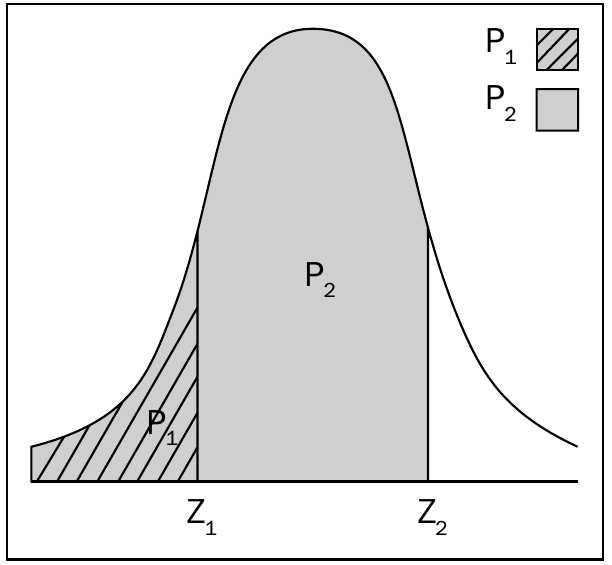
\includegraphics[height=5cm,keepaspectratio=true]{./images/kum0401.png}
	% kum0401.png: 0x0 pixel, 300dpi, 0.00x0.00 cm, bb=
	\caption{Una distribución típica normal con valores $p.$}
	\label{fig:3.7.3}
\end{figure}



Supongamos que $Z_{1}$ y $Z_{2}$ son dos $Z-$estadísticos correspondientes a dos valores de una variable aleatoria y $p_{1}$ y $p_{2}$ son áreas encerradas por la curva de densidad a la derecha de esos valores.

En otras palabras
\begin{align}
	P(X>Z_{1})=p_{1}\\
	P(X>Z_{2})=p_{2}
\end{align}



Entonces, podemos definir un intervalo en el cual encontrar el valor de una variable aleatoria, al cual llamaremos \emph{intervalo de confianza.}


Por ejemplo, para una distribución normal con media $\mu$ y desviación estándar $\sigma,$ el valor de la variable aleatoria estará en el \emph{intervalo} $[\mu-3\sigma,\mu+3\sigma]$ con una \emph{confianza} (probabilidad) del $99\%.$


Para cualquier \emph{estimador} (variable aleatoria) que tenga una distribución normal, uno puede definir un intervalo de confianza si decidimos el nivel de confianza o probabilidad.


Podemos pensar en los \emph{intervalos de confianza} cómo el umbral de los valores aceptados para sostener que la \emph{hipótesis nula} es cierta


Si el valor del estimador vive en este rango, será estadísticamente correcto decir que la hipótesis nula es correcta.


Para definir un intervalo de confianza, se necesita definir antes un \emph{nivel (o probabilidad) de confianza.}  Esta probabilidad necesita ser definida por el investigador dependiendo del contexto.


Digamos que esta probabilidad es $p$. En general, utilizaremos el \emph{nivel de significación}
\begin{align}
	\beta = 1-p,
\end{align}
que representa la probabilidad de que la hipótesis nula no sea correcta. 

$\beta$ es definida por el investigador y usualmente esta en el orden de $0.01$ a $0.1$.



Un concepto importante que aprender aquí es el \emph{valor de probabilidad} o simplemente \emph{valor-}$p$ de un estadístico:  Es la probabilidad de que una variable aleatoria asuma un valor mayor al \emph{valor-}$Z$ (o al \emph{valor-}$t$)
\begin{align}
	p-\texttt{valor}=P\left( X>Z \right)
\end{align}



\begin{figure}
	\centering
	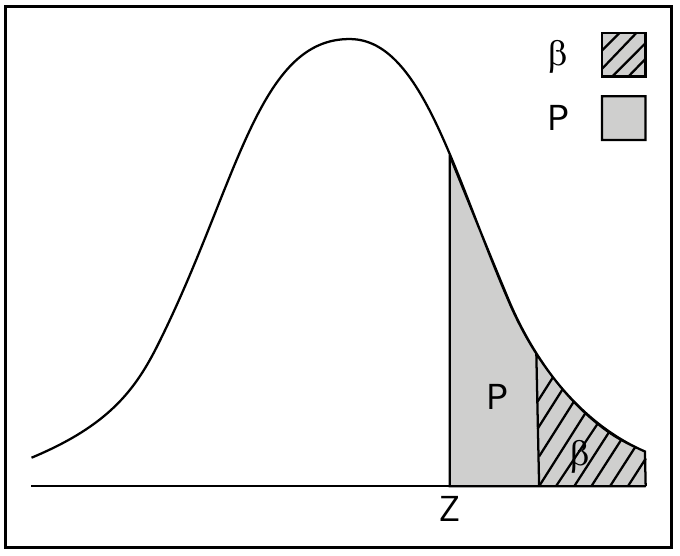
\includegraphics[height=5cm,keepaspectratio=true]{./images/kum0402.png}
	% kum0402.png: 0x0 pixel, 300dpi, 0.00x0.00 cm, bb=
	\caption{Una distribución normal típica con $p-$valores y nivel de significación.}
	\label{fig:3.7.4}
\end{figure}


\subsection{Criterio}
\begin{itemize}
	\item Aceptar la \emph{hipótesis nula y rechazar la alternativa si $p-\texttt{valor}>\beta$}
	\item Aceptar la \emph{hipótesis alternativa y rechazar la nula si $p-\texttt{valor}<\beta$}
\end{itemize}



Debido a la simetría de la distribución normal, existen tres tipos de pruebas de hipótesis:
\begin{enumerate}
	\item Cola izquierda;
	\item cola derecha;
	\item ambas colas.
\end{enumerate}


\subsection{Cola izquierda}
\begin{figure}
	\centering
	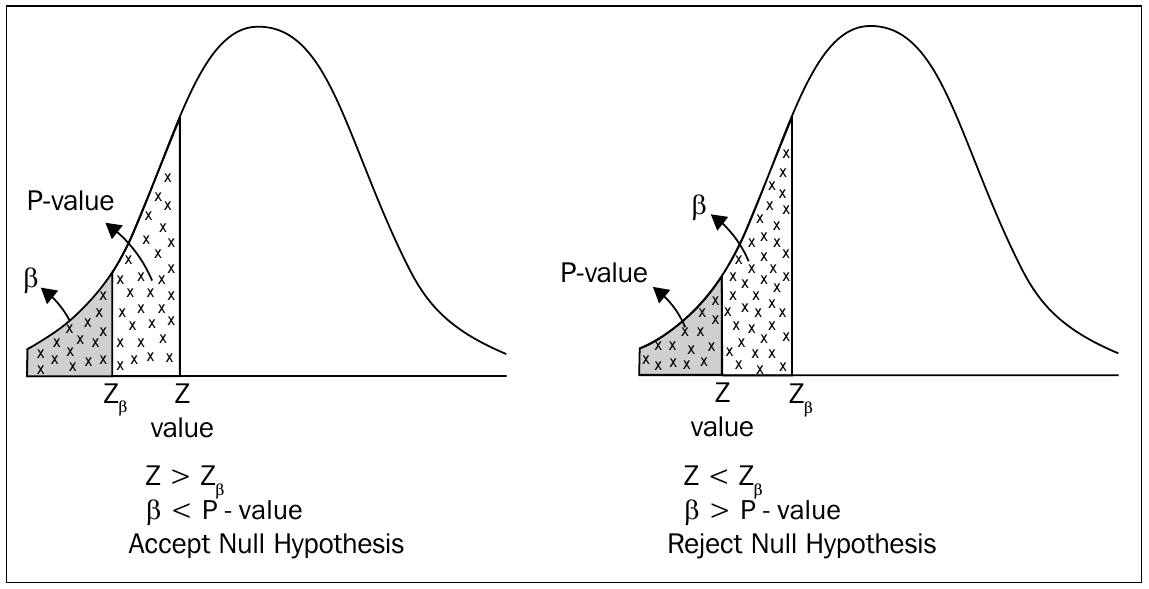
\includegraphics[width=10cm,keepaspectratio=true]{./images/kum0403.png}
	% kum0403.png: 0x0 pixel, 300dpi, 0.00x0.00 cm, bb=
	\caption{Prueba de hipótesis: Cola izquierda}
	\label{fig:3.7.1}
\end{figure}


\subsection{Cola derecha}
\begin{figure}
	\centering
	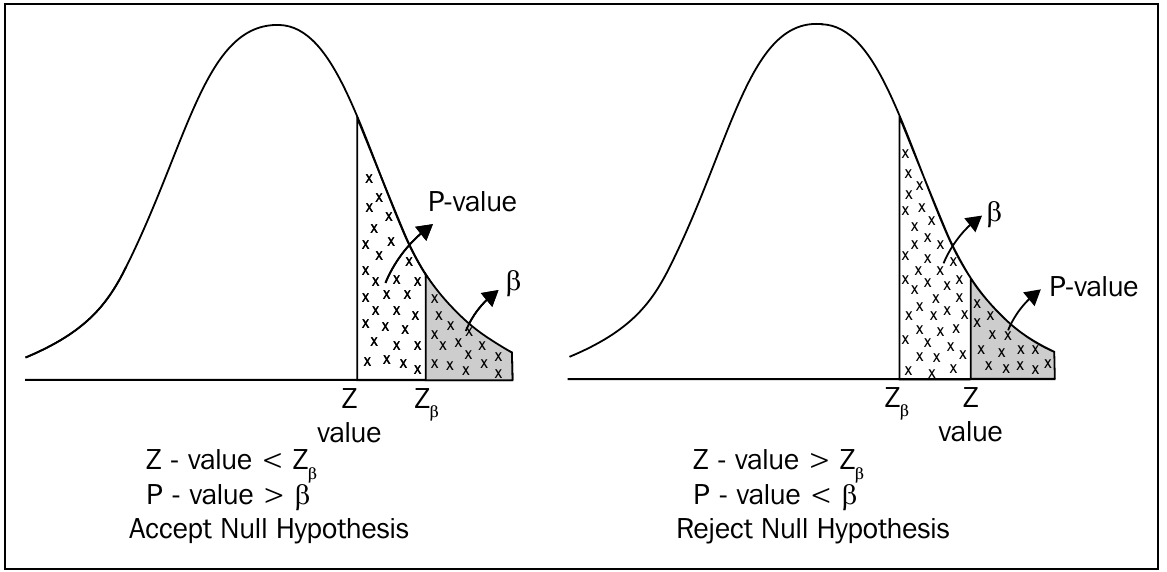
\includegraphics[width=10cm,keepaspectratio=true]{./images/kum0404.png}
	% kum0403.png: 0x0 pixel, 300dpi, 0.00x0.00 cm, bb=
	\caption{Prueba de hipótesis: Cola derecha}
	\label{fig:3.7.2}
\end{figure}


\subsection{Dos colas}
Analizamos ambas colas y si en alguna de las dos colas, falla la respectiva prueba de hipótesis, la prueba de hipótesis se rechaza.

\subsection{Construcción del Intervalo de Confianza para una Media Poblacional}

Formalicemos ahora la construcción explícita del intervalo de confianza para la media poblacional $\mu$ de una sola muestra, distinguiendo el caso en que la desviación estándar poblacional $\sigma$ es conocida del caso, mucho más común en la práctica, en que es desconocida.

\begin{teorema}[Intervalo de confianza para $\mu$ con $\sigma$ conocida]
	Sea $X_1, \ldots, X_n$ una muestra aleatoria de una población normal (o de cualquier población si $n$ es grande, por el TLC) con media $\mu$ desconocida y desviación estándar $\sigma$ \emph{conocida}. Un intervalo de confianza del $(1-\alpha)\times 100\%$ para $\mu$ es:
	\begin{align}
		\bar{X} - Z_{\alpha/2}\frac{\sigma}{\sqrt{n}} \; \leq \; \mu \; \leq \; \bar{X} + Z_{\alpha/2}\frac{\sigma}{\sqrt{n}},
	\end{align}
	donde $Z_{\alpha/2}$ es el cuantil superior $\alpha/2$ de la distribución normal estándar.
\end{teorema}

\begin{teorema}[Intervalo de confianza para $\mu$ con $\sigma$ desconocida]
	Sea $X_1, \ldots, X_n$ una muestra aleatoria de una población normal con $\sigma$ \emph{desconocida}, estimada por la desviación estándar muestral $S$. Reemplazar $\sigma$ por $S$ cambia la distribución exacta del estadístico estandarizado de Normal a $t$ de Student con $n-1$ grados de libertad (Sección 05.04). El intervalo de confianza del $(1-\alpha)\times 100\%$ para $\mu$ es:
	\begin{align}
		\bar{X} - t_{\alpha/2,\,n-1}\frac{S}{\sqrt{n}} \; \leq \; \mu \; \leq \; \bar{X} + t_{\alpha/2,\,n-1}\frac{S}{\sqrt{n}}.
	\end{align}
\end{teorema}

\begin{observacion}[Estructura común: Estimador $\pm$ Margen de Error]
	Ambos intervalos comparten la misma estructura general:
	\begin{align}
		\text{Estimador puntual} \; \pm \; (\text{valor crítico}) \times (\text{error estándar}).
	\end{align}
	Esta estructura --- estimador central, valor crítico de una distribución de referencia, y error estándar del estimador --- se repite en todos los intervalos de confianza que estudiaremos, incluyendo los de diferencia de medias, proporciones y varianzas más adelante en este capítulo.
\end{observacion}

\begin{ejemplo}
	El contenido de líquido en botellas de una embotelladora se distribuye aproximadamente normal. Una muestra de $n=16$ botellas produce $\bar{X}=500.4$ ml.
	\begin{enumerate}
		\item Si se sabe, por especificaciones del fabricante de la máquina, que $\sigma=2$ ml, construya un IC del $95\%$ para $\mu$.
		\item Si en cambio $\sigma$ es desconocida y la muestra produce $S=2.3$ ml, construya el IC del $95\%$ correspondiente (use $t_{15,0.025}\approx 2.131$).
	\end{enumerate}
\end{ejemplo}

\begin{solucion}
	\begin{enumerate}
		\item Con $\sigma=2$ conocida: $\text{SE}=2/\sqrt{16}=0.5$. $\text{IC}_{95\%} = 500.4 \pm 1.96(0.5) = 500.4 \pm 0.98 = [499.42,\ 501.38]$ ml.
		\item Con $S=2.3$ desconocida: $\text{SE}=2.3/\sqrt{16}=0.575$. $\text{IC}_{95\%} = 500.4 \pm 2.131(0.575) = 500.4 \pm 1.225 = [499.18,\ 501.63]$ ml.
	\end{enumerate}
	Nótese que el intervalo basado en $t$ es más ancho que el basado en $Z$, reflejando la incertidumbre adicional de estimar $\sigma$ con $S$ (Sección 05.04).
\end{solucion}


\section*{Problemas}

\subsection*{Enunciados de los problemas}

% Recordar
\begin{problema}
	\label{prob:39c2251}
	Una muestra aleatoria de $n = 36$ estudiantes obtuvo una calificación promedio muestral de $\bar{X} = 78$ puntos en un examen de matemáticas. Suponga que la desviación estándar poblacional es conocida y exactamente igual a $\sigma = 12$ puntos.
	\begin{enumerate}
		\item Construya un intervalo de confianza del 95\% para la media poblacional $\mu$.
		\item Construya un intervalo de confianza del 99\% para la media poblacional $\mu$.
		\item ¿Qué intervalo posee una amplitud mayor? Explique el motivo teórico por el cual la amplitud varía en función del nivel de confianza.
	\end{enumerate}
\end{problema}

% Comprender
\begin{problema}
	\label{prob:8fd99c8}
	Un fabricante de focos LED desea estimar la vida útil promedio de su nueva línea de productos. Toma una muestra aleatoria de $n = 16$ focos y registra un promedio de $\bar{X} = 1,200$ horas con una desviación estándar muestral $s = 80$ horas.
	\begin{enumerate}
		\item ¿Debe utilizar la distribución normal $Z$ o la distribución $t$ de Student para calcular el intervalo de confianza? Argumente su respuesta.
		\item Construya un intervalo de confianza del 95\% para la verdadera vida útil promedio.
		\item Interprete formalmente el intervalo resultante en el contexto del problema.
	\end{enumerate}
\end{problema}

% Aplicar
\begin{problema}
	\label{prob:6af5954}
	Una firma de telecomunicaciones requiere determinar el tiempo promedio real de las llamadas telefónicas de sus abonados corporativos. A partir de una auditoría sobre $n = 100$ llamadas, encuentra una media muestral $\bar{X} = 4.5$ minutos con $s = 2.0$ minutos.
	\begin{enumerate}
		\item Construya el intervalo de confianza del 95\% para la duración media $\mu$.
		\item Determine la magnitud del margen de error de estimación ($E$) actual.
		\item Si la gerencia técnica requiere reducir el margen de error máximo tolerado a $E = 0.2$ minutos al mismo nivel del 95\% de confianza, deduzca y calcule el tamaño de muestra mínimo $n$ necesario.
	\end{enumerate}
\end{problema}

% Analizar
\begin{problema}
	\label{prob:0257f5f}
	\textbf{Deducción analítica de la cota conservadora del tamaño muestral para una proporción Bernoulli:} al diseñar una encuesta para estimar la verdadera proporción poblacional $p \in (0,1)$ con un margen de error máximo admitido $E$ y una confianza $(1-\alpha)$, la expresión algebraica que define el semiancho del intervalo asintótico normal es:
	\begin{align}
		E = Z_{\alpha/2} \sqrt{\frac{p(1-p)}{n}}.
	\end{align}
	\begin{enumerate}
		\item Demuestre rigurosamente, mediante cálculo diferencial, que la varianza muestral teórica de Bernoulli $g(p) = p(1-p)$ alcanza un máximo global absoluto en el dominio $p \in [0,1]$ exactamente en $p = 0.5$.
		\item Demuestre que si no se dispone de información a priori sobre $p$, la fórmula que garantiza que el margen de error nunca excederá el límite $E$ es $n = \left\lceil \dfrac{Z_{\alpha/2}^2}{4 E^2} \right\rceil$.
		\item Una consultora de ciencia de datos requiere estimar la intención de voto hacia una iniciativa pública de salud con un margen de error máximo del $3\%$ ($E = 0.03$) y un nivel de confianza del 95\%. Calcule el número mínimo de encuestas válidas que deberá garantizar.
	\end{enumerate}
\end{problema}

% Evaluar
\begin{problema}
	\label{prob:a3ef454}
	\textbf{Fundamentación epistemológica del intervalo de confianza:} considere la construcción formal del intervalo de confianza empírico $(1-\alpha)$ bajo normalidad, $[L(X), U(X)] = \left[ \bar{X} - Z_{\alpha/2}\frac{\sigma}{\sqrt{n}}, \bar{X} + Z_{\alpha/2}\frac{\sigma}{\sqrt{n}} \right]$. Suponga que, tras tomar la muestra real de 36 estudiantes del Problema \ref{prob:39c2251}, se publica el intervalo numérico $[74.08, 81.92]$.
	\begin{enumerate}
		\item Evalúe por qué, desde la axiomática estricta de la estadística frecuentista, es teóricamente erróneo enunciar que ``la probabilidad de que la verdadera calificación media $\mu$ esté dentro de $[74.08, 81.92]$ es del $95\%$''.
		\item Defina rigurosamente qué significa una ``confianza del 95\%'' desde la perspectiva del muestreo repetido infinito, y contrástelo con el concepto epistemológico del \textbf{intervalo de credibilidad Bayesiano}, donde sí es válido asignar una probabilidad directa al parámetro dados los datos.
	\end{enumerate}
\end{problema}

% Crear
\begin{problema}
	\label{prob:18d6b96}
	Diseñe un problema original que ilustre la dualidad entre intervalos de confianza y pruebas de hipótesis (distinto de calificaciones, focos o llamadas ya vistos): un laboratorio farmacéutico afirma que sus tabletas contienen exactamente $500$ mg de principio activo. Un control de calidad externo toma una muestra de $n=20$ tabletas, con media muestral $\bar{X}=496$ mg y desviación estándar muestral $s=9$ mg. Construya el intervalo de confianza del 95\% para el contenido medio real, determine si el valor afirmado ($500$ mg) está contenido en el intervalo, y explique la conclusión en términos de una prueba de hipótesis bilateral implícita al mismo nivel de significancia.
\end{problema}

\subsection*{Soluciones detalladas}

% Recordar
\begin{solproblema}[prob:39c2251]
	\begin{enumerate}
		\item Con $Z_{0.025}=1.96$ y $\text{SE}=12/\sqrt{36}=2$:
		\begin{align}
			IC_{95\%} = 78 \pm 1.96(2) = 78 \pm 3.92 = [74.08,\;81.92].
		\end{align}
		\item Con $Z_{0.005}=2.576$:
		\begin{align}
			IC_{99\%} = 78 \pm 2.576(2) = 78 \pm 5.152 = [72.85,\;83.15].
		\end{align}
		\item Las amplitudes son $A_{95\%}=7.84$ y $A_{99\%}=10.30$ puntos. El intervalo del 99\% es más amplio: para incrementar la confianza de no dejar fuera al verdadero $\mu$ manteniendo constante la información muestral ($n$), es necesario expandir el margen de captura, abarcando una fracción mayor del área bajo las colas de la normal.
	\end{enumerate}
\end{solproblema}

% Comprender
\begin{solproblema}[prob:8fd99c8]
	\begin{enumerate}
		\item Debe usarse la \textbf{distribución $t$ de Student}: el tamaño de muestra es pequeño ($n=16<30$, lo que impide invocar el TLC) y la desviación estándar poblacional $\sigma$ es desconocida (se sustituye por $s=80$, introduciendo un error de estimación adicional que exige las colas más pesadas de $t$).
		\item Con $\nu=15$ y $t_{0.025,15}=2.131$:
		\begin{align}
			IC_{95\%} = 1{,}200 \pm 2.131\left(\frac{80}{\sqrt{16}}\right) = 1{,}200 \pm 2.131(20) = 1{,}200 \pm 42.62 = [1{,}157.38,\;1{,}242.62] \text{ horas.}
		\end{align}
		\item Si repitiéramos el proceso de muestreo (extraer 16 focos y calcular el intervalo) indefinidamente, en el 95\% de esas muestras la vida útil media verdadera $\mu$ de toda la producción quedaría capturada entre 1,157.38 y 1,242.62 horas.
	\end{enumerate}
\end{solproblema}

% Aplicar
\begin{solproblema}[prob:6af5954]
	\begin{enumerate}
		\item Con $n=100\ge30$ (TLC aplicable) y $Z_{0.025}=1.96$:
		\begin{align}
			IC_{95\%} = 4.5 \pm 1.96\left(\frac{2.0}{\sqrt{100}}\right) = 4.5 \pm 1.96(0.2) = 4.5 \pm 0.392 = [4.108,\;4.892] \text{ min.}
		\end{align}
		\item El margen de error actual es $E=0.392$ minutos.
		\item Partiendo de $E=Z_{\alpha/2}\dfrac{s}{\sqrt{n}}$, despejamos $n=\left(\dfrac{Z_{\alpha/2}\cdot s}{E}\right)^2$. Sustituyendo:
		\begin{align}
			n = \left(\frac{1.96\times2.0}{0.2}\right)^2 = (19.6)^2 = 384.16 \implies n_{\text{óptimo}} = \lceil384.16\rceil = 385 \text{ llamadas.}
		\end{align}
	\end{enumerate}
\end{solproblema}

% Analizar
\begin{solproblema}[prob:0257f5f]
	\begin{enumerate}
		\item Sea $g(p)=p(1-p)=p-p^2$. Derivando: $g'(p)=1-2p=0 \implies p^*=0.5$. Como $g''(p)=-2<0$, es un máximo global, con valor $g(0.5)=0.25$.
		\item Partiendo de $Z_{\alpha/2}\sqrt{p(1-p)/n}\le E$, elevamos al cuadrado: $n\ge Z_{\alpha/2}^2\,p(1-p)/E^2$. Como $p$ es desconocida, sustituimos su cota superior $p(1-p)\le0.25$ (Parte 1) para que la desigualdad valga para cualquier $p$:
		\begin{align}
			n \ge \frac{Z_{\alpha/2}^2(0.25)}{E^2} = \frac{Z_{\alpha/2}^2}{4E^2} \implies n = \left\lceil\frac{Z_{\alpha/2}^2}{4E^2}\right\rceil.
		\end{align}
		\item Con $Z_{0.025}=1.96$ y $E=0.03$:
		\begin{align}
			n = \frac{(1.96)^2}{4(0.03)^2} = \frac{3.8416}{0.0036} \approx 1{,}067.11 \implies n_{\text{óptimo}} = 1{,}068 \text{ encuestas.}
		\end{align}
	\end{enumerate}
\end{solproblema}

% Evaluar
\begin{solproblema}[prob:a3ef454]
	\begin{enumerate}
		\item En el paradigma frecuentista, el parámetro poblacional $\mu$ es una \textbf{constante fija de la naturaleza}, no una variable aleatoria. Una vez extraída la muestra, $\bar{X}$ colapsa al valor observado $\bar{x}=78$, y el intervalo $[74.08,81.92]$ pasa a ser un conjunto numérico completamente determinista. El evento $\mu\in[74.08,81.92]$ ya no tiene ninguna aleatoriedad asociada: o el verdadero $\mu$ está en ese rango (probabilidad $1$) o no lo está (probabilidad $0$). Asignarle el número $0.95$ confunde la probabilidad del \emph{procedimiento} de muestreo con la probabilidad de un parámetro fijo.
		\item \textbf{Interpretación frecuentista correcta:} la confianza del 95\% es una propiedad del \emph{proceso generador del intervalo}, no del intervalo numérico particular. Si se repitiera el muestreo aleatorio un número infinito de veces, generando miles de intervalos $[L(X_k),U(X_k)]$, exactamente el 95\% de esos intervalos aleatorios envolverían al verdadero $\mu$. \textbf{Contraste bayesiano:} en la inferencia Bayesiana, el parámetro $\theta$ sí se trata como una variable aleatoria con distribución a priori $\pi(\theta)$; al condicionar en los datos observados, el Teorema de Bayes produce una distribución a posteriori $\pi(\theta\mid X=x)$, a partir de la cual el intervalo de credibilidad $[A,B]$ satisface $P(A\le\theta\le B\mid X=x)=0.95$ de forma directa y legítima —justo la afirmación que el enfoque frecuentista no puede hacer sobre un intervalo ya calculado.
	\end{enumerate}
\end{solproblema}

% Crear
\begin{solproblema}[prob:18d6b96]
	Con $n=20$ ($\nu=19$), $t_{0.025,19}=2.093$, y $\text{SE}=s/\sqrt{n}=9/\sqrt{20}\approx2.0125$:
	\begin{align}
		IC_{95\%} = 496 \pm 2.093(2.0125) \approx 496 \pm 4.212 = [491.79,\;500.21] \text{ mg.}
	\end{align}
	El valor afirmado ($500$ mg) \textbf{sí está contenido} en el intervalo, ya que $491.79 < 500 < 500.21$. Por la dualidad entre estimación por intervalos y pruebas de hipótesis, si se realizara una prueba $H_0:\mu=500$ vs. $H_a:\mu\neq500$ al nivel $\alpha=0.05$, \textbf{no existiría evidencia suficiente para rechazar $H_0$}: aunque la media muestral ($496$ mg) está por debajo de la especificación, la discrepancia observada es admisible como fluctuación aleatoria del muestreo, y el laboratorio de control de calidad no puede refutar concluyentemente la afirmación del fabricante.
\end{solproblema}

\section{Estimación por intervalo avanzada y tamaño de muestra}

En las secciones previas introducimos de manera intuitiva el concepto de intervalo de confianza y evaluamos estimaciones por intervalo básicas para la media poblacional. Sin embargo, en el análisis estadístico real y en los proyectos de ciencia de datos, rara vez nos limitamos a estudiar una sola población o a contar con parámetros poblacionales conocidos. Con frecuencia debemos comparar dos tratamientos (como en las pruebas A/B de páginas web), evaluar el comportamiento de proporciones o tasas de conversión, analizar la variabilidad o dispersión de los datos y, de manera crítica ante cualquier estudio, calcular con precisión el tamaño de muestra requerido para alcanzar una potencia o precisión determinada.

En esta sección desarrollamos de forma formal, completa y rigurosa la teoría de estimación por intervalo para diferencias de medias, errores estándares, proporciones, varianzas y diseño del tamaño muestral.

\subsection{Estimación de la media y diferencia entre dos medias}

Cuando se estudian dos poblaciones, el interés principal recae en estimar la diferencia de sus medias, $\mu_1 - \mu_2$, a partir de muestras independientes o pareadas extraídas de cada población. El estimador puntual natural y de mínima varianza para esta diferencia es la diferencia de las medias muestrales: $\bar{X}_1 - \bar{X}_2$.

La construcción del intervalo de confianza para $\mu_1 - \mu_2$ depende críticamente del tipo de diseño de muestreo y del conocimiento o suposición sobre las varianzas poblacionales ($\sigma_1^2, \sigma_2^2$).

\begin{teorema}[Caso 1: Muestras independientes con varianzas conocidas]
	Sean $X_{11}, X_{12}, \ldots, X_{1n_1}$ y $X_{21}, X_{22}, \ldots, X_{2n_2}$ dos muestras aleatorias independientes de tamaños $n_1$ y $n_2$ procedentes de poblaciones con medias $\mu_1, \mu_2$ y varianzas conocidas $\sigma_1^2, \sigma_2^2$. Si las poblaciones son normales o los tamaños muestrales son grandes ($n_1, n_2 \geq 30$ por el Teorema del Límite Central), un intervalo de confianza del $(1-\alpha)100\%$ para la diferencia de medias es:
	\begin{align}
		(\bar{X}_1 - \bar{X}_2) - Z_{\alpha/2} \sqrt{\frac{\sigma_1^2}{n_1} + \frac{\sigma_2^2}{n_2}} \leq \mu_1 - \mu_2 \leq (\bar{X}_1 - \bar{X}_2) + Z_{\alpha/2} \sqrt{\frac{\sigma_1^2}{n_1} + \frac{\sigma_2^2}{n_2}},
	\end{align}
	donde $Z_{\alpha/2}$ es el valor crítico de la distribución normal estándar que deja una probabilidad superior de $\alpha/2$.
\end{teorema}

\begin{teorema}[Caso 2: Muestras independientes con varianzas desconocidas pero iguales]
	Si las varianzas poblacionales son desconocidas pero se puede asumir homoscedasticidad ($\sigma_1^2 = \sigma_2^2 = \sigma^2$), combinamos (\emph{pool}) la información de ambas muestras para obtener una estimación ponderada de la varianza común, denotada por la varianza combinada $S_p^2$:
	\begin{align}
		S_p^2 = \frac{(n_1 - 1)S_1^2 + (n_2 - 1)S_2^2}{n_1 + n_2 - 2},
		\label{eq:varianza_combinada}
	\end{align}
	donde $S_1^2$ y $S_2^2$ son las varianzas muestrales insesgadas respectivas. 
	
	El estadístico estandarizado sigue una distribución $t$ de Student con $\nu = n_1 + n_2 - 2$ grados de libertad. El intervalo de confianza del $(1-\alpha)100\%$ para $\mu_1 - \mu_2$ es:
	\begin{align}
		(\bar{X}_1 - \bar{X}_2) \pm t_{\alpha/2, \, n_1+n_2-2} \, S_p \sqrt{\frac{1}{n_1} + \frac{1}{n_2}}.
	\end{align}
\end{teorema}

\begin{teorema}[Caso 3: Muestras independientes con varianzas desconocidas y diferentes (Welch)]
	Cuando las varianzas poblacionales son desconocidas y no es razonable suponer que sean iguales ($\sigma_1^2 \neq \sigma_2^2$), no podemos utilizar la varianza combinada. En este caso (conocido como el problema de Behrens-Fisher), utilizamos las varianzas muestrales individuales y aproximamos la distribución del estadístico mediante la distribución $t$ de Student con los grados de libertad efectivos de Welch-Satterthwaite:
	\begin{align}
		\nu = \frac{\left( \frac{S_1^2}{n_1} + \frac{S_2^2}{n_2} \right)^2}{\frac{\left(S_1^2 / n_1\right)^2}{n_1 - 1} + \frac{\left(S_2^2 / n_2\right)^2}{n_2 - 1}}.
		\label{eq:df_welch}
	\end{align}
	Si $\nu$ no es un entero, se suele redondear hacia abajo al entero inmediato para mantener una actitud conservadora en la cobertura del intervalo. El intervalo del $(1-\alpha)100\%$ resulta en:
	\begin{align}
		(\bar{X}_1 - \bar{X}_2) \pm t_{\alpha/2, \, \nu} \sqrt{\frac{S_1^2}{n_1} + \frac{S_2^2}{n_2}}.
	\end{align}
\end{teorema}

\begin{definicion}[Caso 4: Muestreo pareado o dependiente]
	Cuando las dos muestras están correlacionadas par a par (por ejemplo, mediciones del mismo paciente o del mismo sistema antes y después de un tratamiento), no podemos tratarlas como independientes. En su lugar, reducimos el problema de dos variables a un problema de una sola variable calculando las diferencias individuales:
	\begin{align}
		D_i = X_{1i} - X_{2i}, \quad \text{para } i = 1, 2, \ldots, n.
	\end{align}
	
	Calculamos la media de las diferencias $\bar{D} = \frac{1}{n}\sum D_i$ y la desviación estándar de las diferencias $S_D = \sqrt{\frac{1}{n-1}\sum (D_i - \bar{D})^2}$. El intervalo de confianza del $(1-\alpha)100\%$ para la diferencia media poblacional $\mu_D = \mu_1 - \mu_2$ es:
	\begin{align}
		\bar{D} - t_{\alpha/2, \, n-1} \frac{S_D}{\sqrt{n}} \leq \mu_D \leq \bar{D} + t_{\alpha/2, \, n-1} \frac{S_D}{\sqrt{n}}.
	\end{align}
\end{definicion}

\subsection{Errores estándares de los principales estimadores}

El \emph{Error Estándar} ($SE$, de \emph{Standard Error}) de cualquier estimador puntual $\hat{\theta}$ es la desviación estándar de la distribución muestral de dicho estimador: $SE(\hat{\theta}) = \sqrt{\text{Var}(\hat{\theta})}$. Constituye el bloque de construcción fundamental del margen de error en todo intervalo de confianza.

Para referencia sistemática en ciencia de datos, la Tabla \ref{tab:errores_estandar} resume los errores estándares teóricos y sus estimadores muestrales empíricos para los parámetros más relevantes en inferencia estadística.

\begin{table}[h!]
	\centering
	\begin{tabular}{lccc}
		\hline
		\textbf{Parámetro ($\theta$)} & \textbf{Estimador ($\hat{\theta}$)} & \textbf{Error Estándar Teórico} & \textbf{Estimación del Error Estándar ($\widehat{SE}$)} \\ \hline
		Media una pob. ($\mu$) & $\bar{X}$ & $\frac{\sigma}{\sqrt{n}}$ & $\frac{s}{\sqrt{n}}$ \\ [1.5ex]
		Dif. medias indep. ($\mu_1 - \mu_2$) & $\bar{X}_1 - \bar{X}_2$ & $\sqrt{\frac{\sigma_1^2}{n_1} + \frac{\sigma_2^2}{n_2}}$ & $\sqrt{\frac{S_1^2}{n_1} + \frac{S_2^2}{n_2}}$ \text{ o } $S_p \sqrt{\frac{1}{n_1} + \frac{1}{n_2}}$ \\ [1.5ex]
		Dif. medias pareadas ($\mu_D$) & $\bar{D}$ & $\frac{\sigma_D}{\sqrt{n}}$ & $\frac{S_D}{\sqrt{n}}$ \\ [1.5ex]
		Proporción pobl. ($p$) & $\hat{p} = \frac{X}{n}$ & $\sqrt{\frac{p(1-p)}{n}}$ & $\sqrt{\frac{\hat{p}(1-\hat{p})}{n}}$ \\ [1.5ex]
		Dif. proporciones ($p_1 - p_2$) & $\hat{p}_1 - \hat{p}_2$ & $\sqrt{\frac{p_1(1-p_1)}{n_1} + \frac{p_2(1-p_2)}{n_2}}$ & $\sqrt{\frac{\hat{p}_1(1-\hat{p}_1)}{n_1} + \frac{\hat{p}_2(1-\hat{p}_2)}{n_2}}$ \\ \hline
	\end{tabular}
	\caption{Resumen de errores estándares para los principales estimadores en estadística inferencial.}
	\label{tab:errores_estandar}
\end{table}

\subsection{Estimación de una proporción y diferencia entre dos proporciones}

El estudio de proporciones poblacionales es vital en el análisis de variables categóricas binomiales o de Bernoulli, siendo la base de las métricas de clasificación, tasas de clics en comercio electrónico y porcentajes de preferencia.

\begin{teorema}[Intervalo de confianza para una proporción (Aproximación normal de Wald)]
	Sea $X$ el número de éxitos en una muestra aleatoria de tamaño $n$ de una población Bernoulli con verdadera proporción $p$. El estimador puntual es la proporción muestral $\hat{p} = X/n$. Por el Teorema del Límite Central, si las condiciones de muestra grande se cumplen ($n\hat{p} \geq 5$ y $n(1-\hat{p}) \geq 5$, o de manera más conservadora $\geq 10$), la distribución muestral de $\hat{p}$ es aproximadamente normal.
	
	El intervalo de confianza del $(1-\alpha)100\%$ está dado por:
	\begin{align}
		\hat{p} - Z_{\alpha/2} \sqrt{\frac{\hat{p}(1-\hat{p})}{n}} \leq p \leq \hat{p} + Z_{\alpha/2} \sqrt{\frac{\hat{p}(1-\hat{p})}{n}}.
	\end{align}
\end{teorema}

\begin{observacion}
	Para muestras pequeñas o moderadas, el intervalo de Wald puede presentar coberturas reales notablemente inferiores al nivel $(1-\alpha)$ nominal debido a la asimetría discreta de la distribución binomial. En tales escenarios, los científicos de datos prefieren el \emph{Intervalo de Wilson (o Score)} o la aproximación de Agresti-Coull (añadir 2 éxitos y 2 fracasos ficticios a la muestra, usando $\tilde{n} = n + 4$ y $\tilde{p} = (X+2)/(n+4)$).
\end{observacion}

\begin{teorema}[Intervalo de confianza para la diferencia de dos proporciones]
	Para comparar las tasas de éxito $p_1$ y $p_2$ de dos poblaciones independientes, extraemos muestras de tamaños $n_1$ y $n_2$ y calculamos las proporciones muestrales $\hat{p}_1 = X_1/n_1$ y $\hat{p}_2 = X_2/n_2$. Si ambas muestras son suficientemente grandes ($n_i\hat{p}_i \geq 5$ y $n_i(1-\hat{p}_i) \geq 5$ para $i=1,2$), el intervalo de confianza de nivel $(1-\alpha)100\%$ para $p_1 - p_2$ es:
	\begin{align}
		(\hat{p}_1 - \hat{p}_2) \pm Z_{\alpha/2} \sqrt{\frac{\hat{p}_1(1-\hat{p}_1)}{n_1} + \frac{\hat{p}_2(1-\hat{p}_2)}{n_2}}.
	\end{align}
\end{teorema}

\subsection{Estimación de la varianza y razón de dos varianzas}

En muchas aplicaciones estadísticas, la variabilidad de un proceso es tan trascendental como su promedio. Por ejemplo, en el control de calidad, en finanzas cuantitativas (donde la varianza mide el riesgo o volatilidad del activo) o al verificar los supuestos del ANOVA y la regresión lineal.

\begin{teorema}[Intervalo de confianza para una varianza poblacional $\sigma^2$]
	Sea $X_1, X_2, \ldots, X_n$ una muestra aleatoria de tamaño $n$ de una población distribuida normalmente con media $\mu$ y varianza $\sigma^2$. El estadístico muestral:
	\begin{align}
		\chi^2 = \frac{(n-1)S^2}{\sigma^2}
	\end{align}
	sigue una distribución chi-cuadrada ($\chi^2$) con $n-1$ grados de libertad.
	
	Por lo tanto, un intervalo de confianza del $(1-\alpha)100\%$ para la varianza poblacional $\sigma^2$ (y sacando raíz cuadrada para la desviación estándar $\sigma$) se obtiene despejando los cuantiles de la distribución $\chi^2$:
	\begin{align}
		\frac{(n-1)S^2}{\chi^2_{\alpha/2, \, n-1}} \leq \sigma^2 \leq \frac{(n-1)S^2}{\chi^2_{1-\alpha/2, \, n-1}},
	\end{align}
	donde $\chi^2_{\alpha/2, n-1}$ y $\chi^2_{1-\alpha/2, n-1}$ son los cuantiles superior e inferior de la distribución chi-cuadrada que dejan un área en las colas derechas de $\alpha/2$ y $1-\alpha/2$, respectivamente.
\end{teorema}

\begin{teorema}[Intervalo de confianza para la razón de dos varianzas $\sigma_1^2 / \sigma_2^2$]
	Sean dos muestras aleatorias independientes de tamaños $n_1$ y $n_2$ provenientes de poblaciones normales independientes con varianzas $\sigma_1^2$ y $\sigma_2^2$. El cociente de las varianzas muestrales estandarizadas:
	\begin{align}
		F = \frac{S_1^2 / \sigma_1^2}{S_2^2 / \sigma_2^2} = \left(\frac{S_1^2}{S_2^2}\right)\left(\frac{\sigma_2^2}{\sigma_1^2}\right)
	\end{align}
	sigue una distribución $F$ de Snedecor con $\nu_1 = n_1 - 1$ grados de libertad en el numerador y $\nu_2 = n_2 - 1$ grados de libertad en el denominador.
	
	El intervalo de confianza del $(1-\alpha)100\%$ para el cociente de varianzas poblacionales $\frac{\sigma_1^2}{\sigma_2^2}$ es:
	\begin{align}
		\frac{S_1^2}{S_2^2} \frac{1}{F_{\alpha/2, \, n_1-1, \, n_2-1}} \leq \frac{\sigma_1^2}{\sigma_2^2} \leq \frac{S_1^2}{S_2^2} \frac{1}{F_{1-\alpha/2, \, n_1-1, \, n_2-1}},
	\end{align}
	donde $F_{\alpha/2, \nu_1, \nu_2}$ es el cuantil superior de la distribución $F$. 
	
	Recordando la propiedad de reciprocidad de la distribución $F$, se cumple que $F_{1-\alpha/2, \nu_1, \nu_2} = \frac{1}{F_{\alpha/2, \nu_2, \nu_1}}$, lo que permite simplificar cálculos cuando las tablas estadísticas solo reportan las colas superiores.
\end{teorema}

\subsection{Estimación del tamaño de una muestra}

Uno de los interrogantes de mayor impacto económico y computacional en la ciencia de datos experimental es: \emph{¿cuántos datos necesitamos?} Tomar una muestra demasiado pequeña puede hacer que el estudio carezca de poder para detectar efectos reales, mientras que una muestra excesivamente grande desperdicia recursos financieros, tiempo e infraestructura computacional.

Para determinar el tamaño muestral $n$ adecuado antes de recolectar los datos, debemos especificar tres elementos:
\begin{enumerate}
	\item El \textbf{nivel de confianza nominal $(1-\alpha)$}, que determina el valor crítico ($Z_{\alpha/2}$ o $t_{\alpha/2}$).
	\item El \textbf{margen de error máximo tolerable ($E$)}, que representa la mitad de la longitud deseada del intervalo de confianza.
	\item Una \textbf{estimación previa de la dispersión o variabilidad poblacional} ($\sigma$ para medias, o una proporción esperada $p^*$ para proporciones).
\end{enumerate}

\begin{teorema}[Tamaño de muestra para estimar una media poblacional $\mu$]
	Al estimar la media de una población normal o bajo el Teorema del Límite Central, el margen de error del intervalo de confianza es $E = Z_{\alpha/2} \frac{\sigma}{\sqrt{n}}$. Despejando $n$, obtenemos el tamaño de muestra requerido:
	\begin{align}
		n = \left( \frac{Z_{\alpha/2} \cdot \sigma}{E} \right)^2.
		\label{eq:n_media}
	\end{align}
	Si la varianza poblacional $\sigma^2$ se desconoce, se puede obtener una estimación preliminar mediante: (a) un estudio piloto previo con una muestra pequeña ($n_0 \approx 30$) para usar la desviación estándar muestral $s$; o (b) la regla empírica del rango ($\sigma \approx \frac{\text{Rango estimado}}{4}$ si la población es aproximadamente normal). Siempre que el resultado no sea un número entero, el valor calculado se redondea \emph{hacia el entero superior siguiente} para garantizar que el margen de error final sea menor o igual a $E$.
\end{teorema}

\begin{teorema}[Tamaño de muestra para estimar una proporción poblacional $p$]
	El margen de error para una proporción poblacional utilizando la aproximación normal es $E = Z_{\alpha/2} \sqrt{\frac{p(1-p)}{n}}$. Despejando $n$, obtenemos:
	\begin{align}
		n = \left( \frac{Z_{\alpha/2}}{E} \right)^2 p^* (1 - p^*),
		\label{eq:n_proporcion}
	\end{align}
	donde $p^*$ es una estimación a priori de la proporción real.
	
	\textbf{Caso conservador (sin información previa):} Si no se dispone de ningún dato preliminar sobre el valor probable de $p$, debemos protegernos ante el peor de los casos en cuanto a variabilidad. La función cuadrática $g(p) = p(1-p)$ alcanza su valor máximo absoluto en $p = 0.5$, donde $g(0.5) = 0.5 \times 0.5 = 0.25$. Sustituyendo este máximo en la ecuación anterior, obtenemos la fórmula más segura y conservadora:
	\begin{align}
		n_{\text{max}} = \frac{Z_{\alpha/2}^2}{4 E^2}.
		\label{eq:n_conservador}
	\end{align}
\end{teorema}

\begin{observacion}
	Cuando la población total de estudio es de tamaño finito y relativamente pequeño (denotado por $N$), y la muestra calculada por las fórmulas anteriores representa más del $5\%$ de la población ($n / N > 0.05$), debemos aplicar el \emph{Factor de Corrección por Población Finita} (FCPF). El tamaño muestral ajustado $n_a$ es:
	\begin{align}
		n_a = \frac{n}{1 + \frac{n-1}{N}}.
	\end{align}
	Este ajuste reduce la cantidad de observaciones requeridas sin sacrificar la precisión estipulada.
\end{observacion}

\section{Problemas resueltos de estimación por intervalos y tamaño muestral}

\subsection{Enunciados de los problemas}

\subsubsection*{1. Nivel Fundamental (Sencillos / Directos)}

\begin{problema}
	\label{prob:n_media}
	Un equipo de investigación desea estimar el tiempo promedio en que un usuario permanece interactuando en una plataforma educativa virtual antes de cerrar sesión. Por datos preliminares en plataformas análogas, se sabe que la desviación estándar de la duración de las sesiones ronda los $\sigma = 18$ minutos.
	\begin{enumerate}
		\item ¿Qué tamaño de muestra se requiere para estimar la media poblacional $\mu$ con un margen de error máximo tolerable de $E = 2$ minutos al nivel de confianza del $95\%$?
		\item Si el presupuesto solo permite monitorear un máximo de $n = 150$ sesiones, ¿cuál sería el margen de error real alcanzado con el $95\%$ de confianza?
	\end{enumerate}
\end{problema}

\begin{problema}
	\label{prob:ic_varianza}
	Un equipo de analítica financiera monitorea la volatilidad diaria de un índice bursátil de tecnología. Durante un mes bursátil de $n = 21$ días hábiles, los rendimientos logarítmicos muestran una desviación estándar muestral de $S = 1.45\%$. Asumiendo que los rendimientos diarios siguen una distribución normal, construya un intervalo de confianza del $90\%$ para la verdadera varianza poblacional $\sigma^2$ y para la desviación estándar $\sigma$.
\end{problema}

\begin{problema}
	\label{prob:dif_medias_z_avanzado}
	En una auditoría de rendimiento en centros de datos, se comparan los tiempos de respuesta del procesamiento de consultas en dos clústeres de servidores independientes. De una muestra aleatoria de $n_1 = 50$ consultas en el Clúster 1 se obtuvo un promedio de $\bar{X}_1 = 120.0$ ms con una desviación estándar muestral $S_1 = 15.0$ ms. En el Clúster 2, una muestra de $n_2 = 60$ consultas arrojó $\bar{X}_2 = 112.0$ ms con $S_2 = 12.0$ ms.
	
	Dado que los tamaños muestrales son grandes ($n_1, n_2 \ge 30$), construya un intervalo de confianza paramétrico del $95\%$ para la diferencia en los tiempos promedio de respuesta $\mu_1 - \mu_2$ usando la distribución normal estándar $Z$.
\end{problema}

\subsubsection*{2. Nivel Operativo (Intermedios / De Desarrollo)}

\begin{problema}
	\label{prob:dif_medias_indep_iguales}
	Un ingeniero de ciencia de datos evalúa el tiempo de latencia (en milisegundos) de dos arquitecturas de bases de datos en la nube (Arquitectura A y Arquitectura B) bajo cargas de trabajo similares. Extrae dos muestras aleatorias independientes con los siguientes resultados:
	\begin{itemize}
		\item \textbf{Arquitectura A:} $n_1 = 15$, media muestral $\bar{X}_1 = 48.5$ ms, desviación estándar $S_1 = 6.2$ ms.
		\item \textbf{Arquitectura B:} $n_2 = 12$, media muestral $\bar{X}_2 = 53.8$ ms, desviación estándar $S_2 = 5.8$ ms.
	\end{itemize}
	Asumiendo que las poblaciones son normales y poseen varianzas iguales ($\sigma_1^2 = \sigma_2^2$), construya un intervalo de confianza del $95\%$ para la verdadera diferencia de latencias medias $\mu_1 - \mu_2$.
\end{problema}

\begin{problema}
	\label{prob:dif_proporciones_ab}
	En una prueba A/B para un sitio web de comercio electrónico, se muestran al azar dos versiones de un formulario de pago a los visitantes. De $n_1 = 800$ usuarios expuestos a la Versión A (diseño clásico), $X_1 = 144$ completaron la compra. De $n_2 = 850$ usuarios expuestos a la Versión B (diseño minimalista de un solo paso), $X_2 = 187$ completaron la compra.
	\begin{enumerate}
		\item Construya un intervalo de confianza del $95\%$ para la verdadera diferencia entre las tasas de conversión poblacionales $p_1 - p_2$.
		\item ¿Justifican los datos la decisión de adoptar definitivamente la Versión B?
	\end{enumerate}
\end{problema}

\begin{problema}
	\label{prob:n_proporcion}
	Una firma analítica proyecta realizar una encuesta nacional para determinar la proporción $p$ de hogares urbanos que utilizan servicios de inteligencia artificial generativa en su vida cotidiana.
	\begin{enumerate}
		\item Calcule el tamaño de muestra mínimo requerido para que la estimación tenga un margen de error no mayor a $3\%$ ($E = 0.03$) con un nivel de confianza del $99\%$, asumiendo que no se dispone de ninguna encuesta previa (escenario más conservador).
		\item Suponga que un estudio piloto anterior sugirió que dicha proporción se sitúa en torno al $20\%$ ($\hat{p}^* = 0.20$). ¿Cuántas encuestas se requerirían bajo este nuevo escenario con el mismo nivel de precisión y confianza? ¿Qué porcentaje de ahorro en el tamaño muestral representa contar con esta información previa?
	\end{enumerate}
\end{problema}

\subsubsection*{3. Nivel Analítico (Avanzados / De Conexión)}

\begin{problema}
	\label{prob:dif_medias_welch}
	En un estudio sobre el rendimiento de dos algoritmos de optimización (Algoritmo 1 y Algoritmo 2) aplicados a redes neuronales convolucionales, se midió el tiempo de convergencia en segundos. Como la variabilidad de uno de ellos parece mucho mayor, no se asumen varianzas iguales ($\sigma_1^2 \neq \sigma_2^2$). Los datos obtenidos son:
	\begin{itemize}
		\item \textbf{Algoritmo 1:} $n_1 = 10$, $\bar{X}_1 = 120.4$ s, $S_1 = 18.5$ s.
		\item \textbf{Algoritmo 2:} $n_2 = 14$, $\bar{X}_2 = 105.2$ s, $S_2 = 7.3$ s.
	\end{itemize}
	Construya un intervalo de confianza del $99\%$ para $\mu_1 - \mu_2$ utilizando la aproximación de Welch-Satterthwaite.
\end{problema}

\begin{problema}
	\label{prob:ic_razon_varianzas}
	Para verificar si dos sensores IoT de temperatura industrial fabricados por distintos proveedores tienen exactamente la misma varianza y precisión en sus mediciones, se toman dos muestras independientes:
	\begin{itemize}
		\item \textbf{Proveedor 1:} $n_1 = 16$ mediciones, con varianza muestral $S_1^2 = 0.36$ $^\circ$C$^2$.
		\item \textbf{Proveedor 2:} $n_2 = 13$ mediciones, con varianza muestral $S_2^2 = 0.12$ $^\circ$C$^2$.
	\end{itemize}
	Construya un intervalo de confianza del $98\%$ para la razón de varianzas poblacionales $\dfrac{\sigma_1^2}{\sigma_2^2}$. ¿Existe evidencia estadística para afirmar que un proveedor tiene mayor variabilidad que el otro?
\end{problema}

\subsubsection*{4. Nivel Desafiante (Expertos / Deducción Profunda)}

\begin{problema}
	\label{prob:ic-desaf-fisher}
	\textbf{Deducción del intervalo asintótico exacto para la correlación de Pearson mediante la transformación de Fisher:}
	El coeficiente de correlación lineal muestral $r$ obtenido en una muestra bivariada normal $(X_i, Y_i)$ de tamaño $n$ posee una distribución en el intervalo $[-1, 1]$ que se vuelve extremadamente asimétrica cuando el verdadero parámetro $\rho \to \pm 1$.
	\begin{enumerate}
		\item Explique teóricamente por qué la técnica del error estándar simétrico $r \pm Z_{\alpha/2}\text{SE}(r)$ produce absurdos matemáticos o cobertura deficiente cuando $|\rho|$ es grande en muestras pequeñas o medianas.
		\item La transformación hiperbólica estabilizadora de varianza de Fisher se define por:
		\begin{align}
			Z(r) = \text{artanh}(r) = \frac{1}{2} \ln\left( \frac{1 + r}{1 - r} \right).
		\end{align}
		Demuestre algebraicamente cómo invertir el intervalo simétrico de confianza asintótico para $Z(\rho)$ en la escala transformada ($Z(r) \pm Z_{\alpha/2}\frac{1}{\sqrt{n-3}}$) usando la función tangente hiperbólica $\tanh(z) = \frac{e^{2z}-1}{e^{2z}+1}$ para obtener los límites explícitos $[L_\rho, \, U_\rho]$ en la escala original del coeficiente de correlación.
		\item En un análisis bioinformático sobre expresión génica colineal en $n = 28$ pacientes, se observó un coeficiente de correlación muestral $r = 0.82$. Calcule exactamente el intervalo de confianza del $95\%$ para $\rho$.
	\end{enumerate}
\end{problema}

\begin{problema}
	\label{prob:ic-desaf-delta-method}
	\textbf{El Método Delta para la inferencia por intervalos sobre cocientes de medias:}
	En economía cuantitativa y ciencia de datos, con frecuencia se desea estimar y construir intervalos de confianza para razones o cocientes de parámetros poblacionales $\theta = \dfrac{\mu_Y}{\mu_X}$ (por ejemplo, elasticidad promedio, eficiencia del gasto o retorno sobre costo), a partir de pares de observaciones independientes $(X_1, Y_1), \dots, (X_n, Y_n)$ donde $\mu_X \neq 0$. Se define el estimador cociente natural:
	\begin{align}
		\hat{\theta} = \frac{\bar{Y}}{\bar{X}}.
	\end{align}
	\begin{enumerate}
		\item Utilizando el desarrollo en serie de Taylor de primer orden (o Método Delta multivariado) alrededor del punto exacto $(\mu_X, \mu_Y)$, demuestre rigurosamente que la varianza asintótica de $\hat{\theta}$ está dada por la expresión:
		\begin{align}
			\Var(\hat{\theta}) \approx \frac{1}{n \mu_X^2} \left[ \sigma_Y^2 - 2\theta \sigma_{XY} + \theta^2 \sigma_X^2 \right],
		\end{align}
		donde $\sigma_{XY} = \cov(X, Y)$ es la covarianza poblacional.
		\item A partir del resultado deducido, exprese de forma sistemática cómo construir el intervalo de confianza asintótico del $(1-\alpha)$ para $\theta = \dfrac{\mu_Y}{\mu_X}$ reemplazando los parámetros desconocidos por los momentos muestrales consistentes ($\bar{X}, \bar{Y}, s_X^2, s_Y^2, s_{XY}$).
	\end{enumerate}
\end{problema}


\subsection{Soluciones detalladas}

\subsubsection*{1. Nivel Fundamental (Sencillos / Directos)}

\begin{solproblema}
	\textbf{Parte 1: Tamaño de muestra requerido ($n$).}
	Para un nivel del $95\%$ de confianza, el valor normal tipificado es $Z_{0.025} = 1.96$. La dispersión conocida es $\sigma = 18$ min y el margen de error tolerable es $E = 2$ min.
	
	Sustituimos directamente en la fórmula elemental del tamaño muestral:
	\begin{align}
		n = \left( \frac{Z_{\alpha/2} \cdot \sigma}{E} \right)^2 = \left( \frac{1.96 \times 18}{2} \right)^2 = (1.96 \times 9)^2 = (17.64)^2 = 311.1696.
	\end{align}
	Dado que los tamaños muestrales corresponden a conteos discretos de sesiones enteras y el margen de error debe estrictamente no exceder los 2 minutos, aplicamos la regla del techo redondeando siempre hacia arriba:
	\begin{align}
		n \geq \lceil 311.17 \rceil = 312 \text{ sesiones.}
	\end{align}
	
	\textbf{Parte 2: Margen de error con presupuesto fijo para $n = 150$.}
	Despejamos $E$ de la fórmula del semiancho del intervalo de confianza para la media:
	\begin{align}
		E = Z_{\alpha/2} \frac{\sigma}{\sqrt{n}} = 1.96 \times \frac{18}{\sqrt{150}} = \frac{35.28}{12.2474} \approx 2.8806 \text{ minutos.}
	\end{align}
	Por consiguiente, al limitar la recolección a $150$ sesiones, la precisión del estudio disminuye arrojando un margen de error incrementado de $2.88$ minutos al $95\%$ de confianza.
\end{solproblema}

\begin{solproblema}
	\textbf{Paso 1: Grados de libertad y cuantiles chi-cuadrada.}
	Los grados de libertad del estadístico varianza muestral son $\nu = n - 1 = 21 - 1 = 20$.
	Para un nivel del $90\%$ de confianza ($\alpha = 0.10$), las colas superior e inferior excluyen un área de $\alpha/2 = 0.05$ y $1-\alpha/2 = 0.95$. Consultando las tablas de la distribución $\chi^2$ con $\nu = 20$:
	\begin{align}
		\chi^2_{0.05, \, 20} &= 31.410, \\
		\chi^2_{0.95, \, 20} &= 10.851.
	\end{align}
	
	\textbf{Paso 2: Intervalo para la varianza $\sigma^2$.}
	El numerador de la suma de cuadrados $(n-1)S^2$ es:
	\begin{align}
		(20)(1.45)^2 = 20 \times 2.1025 = 42.05 \text{ (\%}^2\text{).}
	\end{align}
	Sustituyendo en los límites exactos de la distribución $\chi^2$:
	\begin{align}
		\frac{42.05}{31.410} \le \sigma^2 \le \frac{42.05}{10.851} \implies [1.3387, \, 3.8752] \text{ (\%}^2\text{).}
	\end{align}
	
	\textbf{Paso 3: Intervalo para la desviación estándar $\sigma$.}
	Al ser la raíz cuadrada una función estrictamente creciente para reales positivos, tomamos la raíz en todos los términos:
	\begin{align}
		\sqrt{1.3387} \le \sigma \le \sqrt{3.8752} \implies [1.157, \, 1.969] \%.
	\end{align}
	
	\textbf{Interpretación:} Con un $90\%$ de confianza, la verdadera volatilidad diaria del índice bursátil se encuentra acotada entre $1.16\%$ y $1.97\%$.
\end{solproblema}

\begin{solproblema}
	La diferencia entre los promedios muestrales de latencia es:
	\begin{align}
		\hat{D} = \bar{X}_1 - \bar{X}_2 = 120.0 - 112.0 = 8.0 \text{ ms.}
	\end{align}
	Al ser ambas muestras de gran tamaño ($n_1 = 50, n_2 = 60$), el error estándar de la diferencia se calcula y estandariza sin requerir la suposición de varianzas iguales mediante el Teorema del Límite Central:
	\begin{align}
		\text{SE}(\bar{X}_1 - \bar{X}_2) = \sqrt{\frac{S_1^2}{n_1} + \frac{S_2^2}{n_2}} = \sqrt{\frac{15.0^2}{50} + \frac{12.0^2}{60}} = \sqrt{\frac{225.0}{50} + \frac{144.0}{60}} = \sqrt{4.5 + 2.4} = \sqrt{6.9} \approx 2.6268 \text{ ms.}
	\end{align}
	Para un nivel del $95\%$ de confianza ($Z_{0.025} = 1.96$), el margen de error es:
	\begin{align}
		E = 1.96 \times 2.6268 \approx 5.1485 \text{ ms.}
	\end{align}
	El intervalo de confianza paramétrico al 95\% resulta en:
	\begin{align}
		8.0 - 5.1485 \le \mu_1 - \mu_2 \le 8.0 + 5.1485 \implies [2.85, \, 13.15] \text{ ms.}
	\end{align}
	\textbf{Interpretación:} Con un 95\% de confianza, las consultas en el Clúster 1 toman en promedio entre $2.85$ y $13.15$ milisegundos más que en el Clúster 2, probando de forma estadísticamente robusta que el Clúster 2 es más rápido.
\end{solproblema}

\subsubsection*{2. Nivel Operativo (Intermedios / De Desarrollo)}

\begin{solproblema}
	\textbf{Paso 1: Cálculo de la varianza muestral combinada ($S_p^2$).}
	Al asumir normalidad y homoscedasticidad ($\sigma_1^2 = \sigma_2^2$), obtenemos la varianza agrupada ponderada:
	\begin{align}
		S_p^2 &= \frac{(n_1 - 1)S_1^2 + (n_2 - 1)S_2^2}{n_1 + n_2 - 2} = \frac{(15 - 1)(6.2)^2 + (12 - 1)(5.8)^2}{15 + 12 - 2} \\
		&= \frac{14(38.44) + 11(33.64)}{25} = \frac{538.16 + 370.04}{25} = \frac{908.2}{25} = 36.328 \text{ ms}^2.
	\end{align}
	Por ende, la desviación estándar agrupada es $S_p = \sqrt{36.328} \approx 6.027$ ms.
	
	\textbf{Paso 2: Cuantil crítico en la distribución $t$ con $\nu = 25$.}
	Los grados de libertad totales son $\nu = 15 + 12 - 2 = 25$. Para el 95\% de confianza ($\alpha = 0.05$), el valor en tablas es:
	\begin{align}
		t_{0.025, \, 25} = 2.060.
	\end{align}
	
	\textbf{Paso 3: Construcción del intervalo.}
	La diferencia de medias es $\bar{X}_1 - \bar{X}_2 = 48.5 - 53.8 = -5.3$ ms. El margen de error $E$ se calcula como:
	\begin{align}
		E = t_{0.025, \, 25} \cdot S_p \sqrt{\frac{1}{n_1} + \frac{1}{n_2}} = 2.060(6.027) \sqrt{\frac{1}{15} + \frac{1}{12}} = (12.4156) \sqrt{0.1500} = (12.4156)(0.3873) \approx 4.8086 \text{ ms.}
	\end{align}
	El intervalo del $95\%$ para la diferencia de latencias es por tanto:
	\begin{align}
		-5.3 - 4.809 \le \mu_1 - \mu_2 \le -5.3 + 4.809 \implies [-10.11, \, -0.49] \text{ ms.}
	\end{align}
	\textbf{Interpretación:} Al estar todo el intervalo contenido en la región negativa ($[-10.11, -0.49]$) y no tocar el cero, se confirma al 95\% de confianza que la Arquitectura A tiene una latencia media significativamente inferior (es más veloz) que la Arquitectura B.
\end{solproblema}

\begin{solproblema}
	\textbf{Parte 1: Proporciones y error estándar.}
	Las proporciones empíricas de compra (conversión) son:
	\begin{align}
		\hat{p}_1 &= \frac{144}{800} = 0.18 \quad (18\%), \\
		\hat{p}_2 &= \frac{187}{850} = 0.22 \quad (22\%).
	\end{align}
	La diferencia puntual de tasas es $\hat{p}_1 - \hat{p}_2 = 0.18 - 0.22 = -0.04$. Verificamos que todas las cuentas observadas y esperadas de éxitos y fracasos ($144, 656, 187, 663$) son superiores a $10$, por lo que el uso de la aproximación normal asintótica es totalmente válido.
	
	El error estándar de la diferencia se calcula como:
	\begin{align}
		\text{SE}(\hat{p}_1 - \hat{p}_2) &= \sqrt{\frac{\hat{p}_1(1-\hat{p}_1)}{n_1} + \frac{\hat{p}_2(1-\hat{p}_2)}{n_2}} = \sqrt{\frac{0.18(0.82)}{800} + \frac{0.22(0.78)}{850}} \\
		&= \sqrt{\frac{0.1476}{800} + \frac{0.1716}{850}} = \sqrt{0.0001845 + 0.0002019} = \sqrt{0.0003864} \approx 0.01966.
	\end{align}
	Para el $95\%$ de confianza ($Z_{0.025} = 1.96$), el margen de error $E$ es:
	\begin{align}
		E = 1.96 \times 0.01966 \approx 0.0385 \text{ (o 3.85\%).}
	\end{align}
	El intervalo de confianza del $95\%$ para $p_1 - p_2$ resulta en:
	\begin{align}
		-0.04 - 0.0385 \le p_1 - p_2 \le -0.04 + 0.0385 \implies [-0.0785, \, -0.0015].
	\end{align}
	
	\textbf{Parte 2: Decisión sobre el diseño A/B.}
	El intervalo para $p_1 - p_2$ abarca desde $-7.85\%$ hasta $-0.15\%$. Dado que el límite superior es estrictamente inferior a cero, existe certeza estadística al 95\% de confianza de que la tasa de conversión de la Versión B ($p_2$) supera en forma real a la de la Versión A ($p_1$). Por lo tanto, los datos justifican la adopción inmediata de la Versión B.
\end{solproblema}

\begin{solproblema}
	\textbf{Parte 1: Escenario conservador ($\hat{p}^* = 0.5$).}
	Para el 99\% de confianza, el cuantil normal es $Z_{0.005} = 2.576$. El margen de error admitido es $E = 0.03$. Al carecer de encuestas previas, maximizamos la varianza con $p^*(1-p^*) = 0.5(0.5) = 0.25$:
	\begin{align}
		n_{\text{max}} = \frac{Z_{\alpha/2}^2}{4 E^2} = \frac{(2.576)^2}{4 (0.03)^2} = \frac{6.635776}{4 (0.0009)} = \frac{6.635776}{0.0036} = 1,843.27.
	\end{align}
	Aplicando redondeo superior por conteo entero: $n = \lceil 1,843.27 \rceil = 1,844$ hogares en total.
	
	\textbf{Parte 2: Escenario con información previa ($\hat{p}^* = 0.20$).}
	Aprovechando el estudio piloto, la varianza estimada se reduce a $p^*(1-p^*) = 0.20(0.80) = 0.16$:
	\begin{align}
		n = \left( \frac{Z_{\alpha/2}}{E} \right)^2 p^*(1-p^*) = \left( \frac{2.576}{0.03} \right)^2 (0.16) = (85.8667)^2 (0.16) = (7,373.084)(0.16) = 1,179.69.
	\end{align}
	Redondeando al entero superior: $n = \lceil 1,179.69 \rceil = 1,180$ hogares en la encuesta.
	
	\textbf{Evaluación del porcentaje de ahorro:}
	El ahorro absoluto en encuestas al aplicar la información de ciencia de datos a priori es $1,844 - 1,180 = 664$ hogares. La reducción porcentual de costos de recolección es:
	\begin{align}
		\text{Ahorro} = \frac{664}{1,844} \times 100\% \approx 36.01\%.
	\end{align}
\end{solproblema}

\subsubsection*{3. Nivel Analítico (Avanzados / De Conexión)}

\begin{solproblema}
	\textbf{Paso 1: Grados de libertad de Welch-Satterthwaite ($\nu$).}
	Calculamos las varianzas muestrales divididas entre sus respectivos tamaños de grupo:
	\begin{align}
		\frac{S_1^2}{n_1} = \frac{18.5^2}{10} = \frac{342.25}{10} = 34.225, \quad \frac{S_2^2}{n_2} = \frac{7.3^2}{14} = \frac{53.29}{14} \approx 3.8064.
	\end{align}
	Sustituyendo en la aproximación analítica para varianzas heterogéneas:
	\begin{align}
		\nu &= \frac{\left( \dfrac{S_1^2}{n_1} + \dfrac{S_2^2}{n_2} \right)^2}{\dfrac{(S_1^2 / n_1)^2}{n_1 - 1} + \dfrac{(S_2^2 / n_2)^2}{n_2 - 1}} = \frac{(34.225 + 3.8064)^2}{\dfrac{34.225^2}{10 - 1} + \dfrac{3.8064^2}{14 - 1}} = \frac{(38.0314)^2}{\dfrac{1,171.3506}{9} + \dfrac{14.4887}{13}} \\
		&= \frac{1,446.3874}{130.1501 + 1.1145} = \frac{1,446.3874}{131.2646} \approx 11.0188.
	\end{align}
	Tomando la parte entera conservadora para no sobreestimar la confianza, obtenemos $\nu = 11$ grados de libertad.
	
	\textbf{Paso 2: Valor crítico en la tabla de Student y error estándar.}
	Para el 99\% de confianza ($\alpha = 0.01 \implies \alpha/2 = 0.005$) en $\nu = 11$, el valor en tablas es $t_{0.005, \, 11} = 3.106$.
	El error estándar de la diferencia entre promedios es:
	\begin{align}
		\text{SE}(\bar{X}_1 - \bar{X}_2) = \sqrt{\frac{S_1^2}{n_1} + \frac{S_2^2}{n_2}} = \sqrt{34.225 + 3.8064} = \sqrt{38.0314} \approx 6.1670 \text{ s.}
	\end{align}
	
	\textbf{Paso 3: Construcción e interpretación del intervalo al 99\%:}
	La diferencia muestral observada es $\hat{D} = 120.4 - 105.2 = 15.2$ s. El margen de error $E$ resulta en:
	\begin{align}
		E = 3.106 \times 6.1670 \approx 19.155 \text{ s.}
	\end{align}
	El intervalo al 99\% para $\mu_1 - \mu_2$ es:
	\begin{align}
		15.2 - 19.155 \le \mu_1 - \mu_2 \le 15.2 + 19.155 \implies [-3.955, \, 34.355] \text{ s.}
	\end{align}
	Al cruzar por el cero de negativo a positivo ($[-3.96, 34.36]$), no podemos declarar que el Algoritmo 2 sea significativamente más veloz que el Algoritmo 1 al 99\% de confianza.
\end{solproblema}

\begin{solproblema}
	\textbf{Paso 1: Grados de libertad y puntos críticos de Fisher ($F$).}
	Los grados de libertad del numerador y denominador son $\nu_1 = n_1 - 1 = 15$ y $\nu_2 = n_2 - 1 = 12$.
	Para una confianza del $98\%$ ($\alpha = 0.02 \implies \alpha/2 = 0.01$), el cuantil superior en la tabla $F$ es:
	\begin{align}
		F_{0.01, \, 15, \, 12} = 3.96.
	\end{align}
	Por la propiedad de reciprocidad geométrica para intercambiar grados de libertad, el cuantil inferior es:
	\begin{align}
		F_{0.99, \, 15, \, 12} = \frac{1}{F_{0.01, \, 12, \, 15}} = \frac{1}{3.67} \approx 0.2725.
	\end{align}
	
	\textbf{Paso 2: Cálculo del intervalo para la razón poblacional $\dfrac{\sigma_1^2}{\sigma_2^2}$.}
	El cociente empírico entre las varianzas muestrales observadas es:
	\begin{align}
		\frac{S_1^2}{S_2^2} = \frac{0.36}{0.12} = 3.00.
	\end{align}
	Sustituimos en la fórmula general del intervalo para razón de dispersiones:
	\begin{align}
		\frac{S_1^2 / S_2^2}{F_{0.01, \, 15, \, 12}} \le \frac{\sigma_1^2}{\sigma_2^2} \le \frac{S_1^2 / S_2^2}{F_{0.99, \, 15, \, 12}} \implies \frac{3.00}{3.96} \le \frac{\sigma_1^2}{\sigma_2^2} \le \frac{3.00}{0.2725} \implies [0.7576, \, 11.009].
	\end{align}
	\textbf{Interpretación y conclusión docimásica:} El intervalo del 98\% para el cociente de varianzas se extiende de $0.758$ a $11.009$. Puesto que la razón de equivalencia exacta ($1.0$) yace cómodamente en el interior de los límites empíricos, los datos demuestran que no existe evidencia suficiente al $98\%$ para concluir que el sensor del Proveedor 1 tenga una variabilidad superior o inferior que el del Proveedor 2.
\end{solproblema}

\subsubsection*{4. Nivel Desafiante (Expertos / Deducción Profunda)}

\begin{solproblema}
	\begin{enumerate}
		\item \textbf{Limitaciones teóricas de la aproximación simétrica en $r$:}
		El coeficiente de correlación $r$ está estrictamente delimitado en su dominio al espacio compacto $[-1, 1]$. Cuando la verdadera correlación poblacional es fuerte (por ejemplo, $\rho = 0.85$), la distribución en el muestreo de $r$ se comprime violentamente contra la cota superior $+1$, generando una fuerte asimetría negativa con cola izquierda extendida. Si en este escenario utilizáramos la fórmula ingenua $r \pm Z_{\alpha/2}\text{SE}(r)$, el límite superior del intervalo superaría con frecuencia el valor $+1$ (absurdo axiomático en correlaciones), y la tasa de cobertura real caería drásticamente por debajo del nominal $95\%$ debido a que la varianza exacta del estimador $r$ depende pesadamente del propio parámetro $\rho$: $\Var(r) \approx \dfrac{(1-\rho^2)^2}{n}$.
		
		\item \textbf{Inversión de la transformación hiperbólica de Fisher:}
		Sir Ronald Fisher dedujo que al aplicar al estimador $r$ el arcotangente hiperbólico, la variable transformada $Z(r) = \text{artanh}(r) = \dfrac{1}{2}\ln\left(\dfrac{1+r}{1-r}\right)$ sigue una distribución asintóticamente normal cuya media es $Z(\rho)$ y, lo que es fundamental, \textbf{cuya varianza es estabilizada en la constante independiente del parámetro $\dfrac{1}{n-3}$}:
		\begin{align}
			Z(r) \sim N\left( \frac{1}{2}\ln\left(\frac{1+\rho}{1-\rho}\right), \; \frac{1}{n-3} \right).
		\end{align}
		Por lo tanto, el intervalo asintótico simétrico al $(1-\alpha)$ para el parámetro $Z(\rho)$ en la escala transformada se escribe sin error:
		\begin{align}
			\left[ Z_L, \, Z_U \right] = \left[ Z(r) - Z_{\alpha/2} \frac{1}{\sqrt{n-3}}, \; Z(r) + Z_{\alpha/2} \frac{1}{\sqrt{n-3}} \right].
		\end{align}
		Dado que la función tangente hiperbólica $\tanh(z) = \dfrac{e^{2z}-1}{e^{2z}+1}$ es una función estrictamente monótona creciente y continua para todo $z \in \mathbb{R}$, preserva las desigualdades de probabilidad algebraicas al ser aplicada a todos los miembros:
		\begin{align}
			Z_L \le Z(\rho) \le Z_U \iff \tanh(Z_L) \le \tanh\left(\text{artanh}(\rho)\right) \le \tanh(Z_U) \iff \tanh(Z_L) \le \rho \le \tanh(Z_U).
		\end{align}
		Así se deducen los límites exactos en la escala original:
		\begin{align}
			[L_\rho, \, U_\rho] = \left[ \tanh(Z_L), \; \tanh(Z_U) \right].
		\end{align}
		
		\item \textbf{Cálculo numérico para el estudio bioinformático ($r = 0.82, n = 28$):}
		Evaluamos la transformación de Fisher en $r = 0.82$:
		\begin{align}
			Z(0.82) = \frac{1}{2} \ln\left( \frac{1 + 0.82}{1 - 0.82} \right) = \frac{1}{2} \ln\left( \frac{1.82}{0.18} \right) = \frac{1}{2} \ln(10.1111) = \frac{1}{2}(2.31363) \approx 1.1568.
		\end{align}
		El error estándar constante en la escala $Z$ para $n = 28$ es:
		\begin{align}
			\text{SE}_Z = \frac{1}{\sqrt{n - 3}} = \frac{1}{\sqrt{28 - 3}} = \frac{1}{\sqrt{25}} = \frac{1}{5} = 0.2000.
		\end{align}
		Para 95\% de confianza ($Z_{0.025} = 1.96$), construimos los límites intermedios $Z_L$ y $Z_U$:
		\begin{align}
			Z_L &= 1.1568 - 1.96(0.2000) = 1.1568 - 0.3920 = 0.7648, \\
			Z_U &= 1.1568 + 1.96(0.2000) = 1.1568 + 0.3920 = 1.5488.
		\end{align}
		Aplicando la función de inversión monótona $\tanh(z)$ a cada límite para regresar al espacio $[-1, 1]$:
		\begin{align}
			L_\rho &= \tanh(0.7648) = \frac{e^{2(0.7648)} - 1}{e^{2(0.7648)} + 1} = \frac{e^{1.5296} - 1}{e^{1.5296} + 1} = \frac{4.6163 - 1}{4.6163 + 1} = \frac{3.6163}{5.6163} \approx 0.6439. \\
			U_\rho &= \tanh(1.5488) = \frac{e^{2(1.5488)} - 1}{e^{2(1.5488)} + 1} = \frac{e^{3.0976} - 1}{e^{3.0976} + 1} = \frac{22.1448 - 1}{22.1448 + 1} = \frac{21.1448}{23.1448} \approx 0.9136.
		\end{align}
		El intervalo asintótico exacto al 95\% de confianza para la verdadera correlación poblacional en expresión génica es:
		\begin{align}
			IC_{95\%}(\rho) = [0.6439, \; 0.9136].
		\end{align}
		Obsérvese cómo el intervalo obtenido es lógicamente asimétrico alrededor del estimador puntual ($0.82 - 0.6439 = 0.1761$ de distancia izquierda frente a $0.9136 - 0.82 = 0.0936$ de distancia derecha), respetando perfectamente la frontera natural de $+1$.
	\end{enumerate}
\end{solproblema}

\begin{solproblema}
	\begin{enumerate}
		\item \textbf{Deducción algebraico-diferencial del Método Delta para cocientes:}
		Sea la función objetivo no lineal de dos variables $g(u, v) = \dfrac{v}{u}$, evaluada sobre el vector aleatorio de medias muestrales $(\bar{X}, \bar{Y})$ cuyo verdadero parámetro de esperanza es $\boldsymbol{\mu} = (\mu_X, \mu_Y)$.
		
		Desarrollamos la serie de Taylor bivariada de primer orden de $g(\bar{X}, \bar{Y})$ alrededor del punto paramétrico $(\mu_X, \mu_Y)$:
		\begin{align}
			g(\bar{X}, \bar{Y}) \approx g(\mu_X, \mu_Y) + \left. \frac{\partial g}{\partial u} \right|_{(\mu_X, \mu_Y)} (\bar{X} - \mu_X) + \left. \frac{\partial g}{\partial v} \right|_{(\mu_X, \mu_Y)} (\bar{Y} - \mu_Y).
		\end{align}
		Calculamos las derivadas parciales exactas evaluadas en el punto central:
		\begin{align}
			\frac{\partial g}{\partial u} &= \frac{\partial}{\partial u}\left( \frac{v}{u} \right) = -\frac{v}{u^2} \implies \left. \frac{\partial g}{\partial u} \right|_{(\mu_X, \mu_Y)} = -\frac{\mu_Y}{\mu_X^2} = -\frac{\theta}{\mu_X}. \\
			\frac{\partial g}{\partial v} &= \frac{\partial}{\partial v}\left( \frac{v}{u} \right) = \frac{1}{u} \implies \left. \frac{\partial g}{\partial v} \right|_{(\mu_X, \mu_Y)} = \frac{1}{\mu_X}.
		\end{align}
		Sustituyendo en la expansión lineal tipificada del estimador cociente $\hat{\theta}$:
		\begin{align}
			\hat{\theta} = \frac{\bar{Y}}{\bar{X}} \approx \theta - \frac{\theta}{\mu_X}(\bar{X} - \mu_X) + \frac{1}{\mu_X}(\bar{Y} - \mu_Y).
		\end{align}
		Para obtener la varianza asintótica de $\hat{\theta}$, aplicamos el operador varianza a la aproximación lineal. Recordando que para cualquier combinación lineal $\Var(aW_1 + bW_2) = a^2\Var(W_1) + b^2\Var(W_2) + 2ab\cov(W_1, W_2)$ y que el término constante $\theta$ tiene varianza nula:
		\begin{align}
			\Var(\hat{\theta}) \approx \left( -\frac{\theta}{\mu_X} \right)^2 \Var(\bar{X}) + \left( \frac{1}{\mu_X} \right)^2 \Var(\bar{Y}) + 2\left( -\frac{\theta}{\mu_X} \right)\left( \frac{1}{\mu_X} \right) \cov(\bar{X}, \bar{Y}).
		\end{align}
		Por propiedades del muestreo independiente y apareado i.i.d. de tamaño $n$, las varianzas y covarianzas de los promedios muestrales son:
		\begin{align}
			\Var(\bar{X}) = \frac{\sigma_X^2}{n}, \quad \Var(\bar{Y}) = \frac{\sigma_Y^2}{n}, \quad \cov(\bar{X}, \bar{Y}) = \frac{\sigma_{XY}}{n}.
		\end{align}
		Sustituyendo estas varianzas muestrales en la ecuación y extrayendo el factor común $1 / (n \mu_X^2)$:
		\begin{align}
			\Var(\hat{\theta}) \approx \frac{\theta^2}{\mu_X^2} \left( \frac{\sigma_X^2}{n} \right) + \frac{1}{\mu_X^2} \left( \frac{\sigma_Y^2}{n} \right) - \frac{2\theta}{\mu_X^2} \left( \frac{\sigma_{XY}}{n} \right) = \frac{1}{n \mu_X^2} \left[ \sigma_Y^2 - 2\theta \sigma_{XY} + \theta^2 \sigma_X^2 \right].
		\end{align}
		Queda demostrado formalmente el resultado fundamental del Método Delta para cocientes algebraicos de promedios.
		
		\item \textbf{Procedimiento sistemático de estimación por intervalos en la práctica:}
		Dado que en la realidad empírica de ciencia de datos los parámetros teóricos $(\mu_X, \sigma_X^2, \sigma_Y^2, \sigma_{XY}, \theta)$ se desconocen, para construir el intervalo de confianza $(1-\alpha)$ se sigue este protocolo secuencial:
		\begin{itemize}
			\item Se estiman puntualmente los promedios y varianzas muestrales insesgadas: $\bar{X}, \bar{Y}, s_X^2, s_Y^2$, y se calcula la covarianza muestral de los pares dados:
			\begin{align}
				s_{XY} = \frac{1}{n-1} \sum_{i=1}^n (X_i - \bar{X})(Y_i - \bar{Y}).
			\end{align}
			\item Se evalúa la razón puntual central $\hat{\theta} = \dfrac{\bar{Y}}{\bar{X}}$.
			\item Se sustituyen las estimaciones en la fórmula deducida para obtener el error estándar consistente ($\text{SE}_{\hat{\theta}}$):
			\begin{align}
				\text{SE}(\hat{\theta}) = \sqrt{ \frac{1}{n \bar{X}^2} \left[ s_Y^2 - 2\hat{\theta} s_{XY} + \hat{\theta}^2 s_X^2 \right] }.
			\end{align}
			\item Finalmente, por normalidad asintótica del estimador linealizado al $n \to \infty$, el intervalo de confianza al $(1-\alpha)$ para la razón poblacional $\theta$ se formula como:
			\begin{align}
				IC_{(1-\alpha)}(\theta) = \hat{\theta} \pm Z_{\alpha/2} \cdot \text{SE}(\hat{\theta}) = \frac{\bar{Y}}{\bar{X}} \pm Z_{\alpha/2} \sqrt{ \frac{1}{n \bar{X}^2} \left[ s_Y^2 - 2\hat{\theta} s_{XY} + \hat{\theta}^2 s_X^2 \right] }.
			\end{align}
		\end{itemize}
	\end{enumerate}
\end{solproblema}


%%%%%%%%%%%%%%%%%%%%%%%%%%%%%%
% UNIDAD 6 DEL TEMARIO
\chapter{Docimasia (Pruebas de Hipótesis)}
\section{Elementos de prueba de hipótesis}

En la prueba de hipótesis, asumimos una premisa inicial (generalmente relacionada con el valor del estimador) denominada \emph{hipótesis nula} y trataremos de ver si es cierta o no aplicando técnicas estadísticas.

Tenemos otra premisa llamada \emph{hipótesis alternativa}, la cuál es la negación de la hipótesis nula.

\subsection{Hipótesis nula vs. alternativa}

Cuando alguien está haciendo una \emph{investigación} cuantitativa para calibrar el valor de un estimador, el \emph{valor conocido} del parámetro se toma como \emph{hipótesis nula}, mientras que el \emph{nuevo valor} encontrado (de la investigación) se toma como la \emph{hipótesis alternativa}.

En nuestro caso (encontrar la edad media de nuestra ciudad), un investigador puede afirmar que la edad es \emph{menor que 35}. Esto puede servir como la \emph{hipótesis nula}.

Si una nueva agencia afirma que es \emph{mayor que 35}, entonces se puede denominar como la \emph{hipótesis alternativa}.

\subsection{Notación formal}

Denotamos las hipótesis como:
\begin{itemize}
	\item $H_0$: Hipótesis nula (afirmación que se asume verdadera inicialmente)
	\item $H_a$ o $H_1$: Hipótesis alternativa (afirmación que contradice a $H_0$)
\end{itemize}

\begin{ejemplo}
	Un fabricante de cereales afirma que el peso promedio de sus cajas es de 500 gramos. Un inspector de calidad sospecha que el peso es menor.

	\begin{align}
		H_0: \mu &= 500 \text{ g} \\
		H_a: \mu &< 500 \text{ g}
	\end{align}
\end{ejemplo}

\subsection{Tipos de pruebas de hipótesis}

Dependiendo de la hipótesis alternativa, las pruebas pueden ser:

\begin{enumerate}
	\item \textbf{Prueba de cola izquierda:}
	\begin{align}
		H_0: \mu &= \mu_0 \\
		H_a: \mu &< \mu_0
	\end{align}

	\item \textbf{Prueba de cola derecha:}
	\begin{align}
		H_0: \mu &= \mu_0 \\
		H_a: \mu &> \mu_0
	\end{align}

	\item \textbf{Prueba de dos colas:}
	\begin{align}
		H_0: \mu &= \mu_0 \\
		H_a: \mu &\neq \mu_0
	\end{align}
\end{enumerate}

\subsection{Errores en pruebas de hipótesis}

Al tomar decisiones basadas en datos muestrales, podemos cometer dos tipos de errores:

\begin{definicion}[Error tipo I]
	Rechazar la hipótesis nula cuando en realidad es verdadera. La probabilidad de cometer este error se denota como $\alpha$ (nivel de significación):
	\begin{align}
		\alpha = P(\text{Rechazar } H_0 | H_0 \text{ es verdadera})
	\end{align}
\end{definicion}

\begin{definicion}[Error tipo II]
	No rechazar la hipótesis nula cuando en realidad es falsa. La probabilidad de cometer este error se denota como $\beta$:
	\begin{align}
		\beta = P(\text{No rechazar } H_0 | H_0 \text{ es falsa})
	\end{align}
\end{definicion}

\begin{observacion}
	La \emph{potencia} de una prueba es la probabilidad de rechazar correctamente una hipótesis nula falsa:
	\begin{align}
		\text{Potencia} = 1 - \beta = P(\text{Rechazar } H_0 | H_0 \text{ es falsa})
	\end{align}
\end{observacion}

\subsection{Potencia y tamaño de muestra}

La \emph{potencia} de una prueba no es un valor fijo: depende del tamaño real del efecto que se desea detectar ($\mu_a - \mu_0$), del tamaño de muestra $n$ y del nivel de significación $\alpha$ elegido. En el diseño experimental, el investigador puede fijar de antemano tanto $\alpha$ como la potencia deseada $1-\beta$ para determinar cuántas observaciones $n$ debe recolectar.

\begin{teorema}[Tamaño de muestra para una potencia objetivo, prueba $Z$ de una cola]
	Sea una prueba de hipótesis sobre la media de una población normal con desviación estándar conocida $\sigma$, de la forma $H_0: \mu = \mu_0$ contra $H_a: \mu > \mu_0$ (o su análoga de cola izquierda). Si se desea que la prueba alcance una potencia $1-\beta$ para detectar un efecto real de tamaño $\mu_a \neq \mu_0$ al nivel de significación $\alpha$, el tamaño de muestra mínimo requerido es:
	\begin{align}
		n = \left( \frac{(Z_\alpha + Z_\beta)\, \sigma}{\mu_a - \mu_0} \right)^2,
		\label{eq:tam_muestra_potencia}
	\end{align}
	donde $Z_\alpha$ y $Z_\beta$ son los cuantiles superiores de la normal estándar correspondientes a $\alpha$ y $\beta$ respectivamente. Para una prueba de dos colas, se reemplaza $Z_\alpha$ por $Z_{\alpha/2}$.
\end{teorema}

\begin{observacion}
	La fórmula \eqref{eq:tam_muestra_potencia} revela relaciones fundamentales de diseño experimental:
	\begin{itemize}
		\item A mayor tamaño de efecto deseado ($\mu_a - \mu_0$ más grande), \textbf{menor} es el tamaño de muestra necesario: los efectos grandes son más fáciles de detectar.
		\item A mayor potencia exigida (por ejemplo, pasar de $1-\beta = 0.80$ a $1-\beta = 0.95$), \textbf{mayor} es el tamaño de muestra requerido, pues $Z_\beta$ crece.
		\item A menor $\alpha$ (una prueba más estricta contra falsos positivos), también \textbf{mayor} es el tamaño de muestra requerido, pues $Z_\alpha$ crece.
	\end{itemize}
	Esto formaliza la intuición de que existe un \emph{trade-off} triangular entre el error Tipo I, el error Tipo II y el costo (tamaño de muestra) de un experimento.
\end{observacion}


% ==============================================================================
% SECCIÓN 07.01: FUNDAMENTOS DE PRUEBAS DE HIPÓTESIS ($H_0$ VS $H_1$, ERRORES Y POTENCIA)
% ==============================================================================

\subsection*{Enunciados de los problemas --- Sección 07.01}

\subsubsection*{Nivel Fundamental}

\begin{problema}
	\label{prob:7.1.1}
	Un fabricante de baterías afirma que la vida media de su producto es de $\mu_0 = 500$ horas. Un laboratorio independiente sospecha que la vida media real es \emph{menor}. Formule las hipótesis nula ($H_0$) y alternativa ($H_a$), e identifique si la prueba es de cola izquierda, derecha o de dos colas.
\end{problema}

\begin{problema}
	\label{prob:7.1.2}
	Un examen de detección de una enfermedad rara se diseña con $H_0:$ ``el paciente está sano'' contra $H_a:$ ``el paciente está enfermo''. Describa en palabras qué representa el Error Tipo I y el Error Tipo II en este contexto médico específico, y razone cuál de los dos errores tiene consecuencias prácticas más graves.
\end{problema}

\begin{problema}
	\label{prob:7.1.3}
	En una prueba de hipótesis de cola derecha se obtiene un valor $p = 0.023$ con un nivel de significación $\alpha = 0.05$. Aplique la regla de decisión basada en el valor $p$ e indique la conclusión formal (rechazar o no rechazar $H_0$).
\end{problema}

\subsubsection*{Nivel Operativo}

\begin{problema}
	\label{prob:7.1.4}
	Una cadena de restaurantes afirma que el tiempo promedio de espera es de $\mu_0 = 12$ minutos. Una muestra de $n = 49$ clientes reporta $\bar{x} = 12.9$ minutos con desviación estándar poblacional conocida $\sigma = 2.8$ minutos. Formule las hipótesis para una prueba de dos colas, calcule el estadístico $Z$, obtenga el valor $p$ correspondiente, y decida al nivel $\alpha = 0.05$.
\end{problema}

\begin{problema}
	\label{prob:7.1.5}
	Para la prueba $H_0: \mu = 100$ contra $H_a: \mu > 100$ con $\sigma = 15$ conocida y $n = 25$, la región de rechazo al nivel $\alpha = 0.05$ es $\bar{X} > 104.93$. Suponga que el valor real de la media poblacional es $\mu_a = 108$. Calcule la probabilidad del Error Tipo II ($\beta$) y la potencia de la prueba ($1-\beta$).
\end{problema}

\begin{problema}
	\label{prob:7.1.6}
	Continuando el contexto del Problema \ref{prob:7.1.5} ($\sigma=15$, $\mu_0=100$, $\mu_a=108$, $\alpha=0.05$ de una cola), determine el tamaño de muestra mínimo $n$ necesario para que la prueba alcance una potencia de $1-\beta = 0.90$ (use $Z_{0.10} = 1.282$).
\end{problema}

\subsubsection*{Nivel Analítico}

\begin{problema}
	\label{prob:7.1.7}
	Para la prueba $H_0: \mu=\mu_0$ contra $H_a: \mu>\mu_0$ con $\sigma$ conocida y tamaño de muestra $n$ fijo, deduzca la expresión general de la función de potencia $\text{Pot}(\mu_a) = 1-\beta(\mu_a)$ como función del verdadero valor $\mu_a$, expresándola en términos de la función de distribución normal estándar $\Phi(\cdot)$. Analice y justifique el comportamiento de $\text{Pot}(\mu_a)$ en los límites $\mu_a \to \mu_0$ y $\mu_a \to \infty$.
\end{problema}

\begin{problema}
	\label{prob:7.1.8}
	Un científico de datos ejecuta $m = 20$ pruebas de hipótesis estadísticamente independientes sobre distintas hipótesis nulas verdaderas, cada una al nivel individual $\alpha = 0.05$. Deduzca la fórmula general de la Tasa de Error Familiar (\emph{Family-Wise Error Rate}, FWER) —la probabilidad de cometer al menos un Error Tipo I en el conjunto completo de pruebas— y calcule su valor numérico. Proponga y justifique el nivel de significación individual corregido $\alpha^*$ (corrección de Bonferroni) necesario para mantener el FWER global en $0.05$.
\end{problema}

\subsubsection*{Nivel Desafiante}

\begin{problema}
	\label{prob:7.1.9}
	\textbf{Lema de Neyman-Pearson y optimalidad del test $Z$:} Sea $X_1,\ldots,X_n$ una muestra iid $N(\mu,\sigma^2)$ con $\sigma^2$ conocida, y considere el contraste \emph{simple contra simple} $H_0: \mu=\mu_0$ contra $H_a: \mu=\mu_1$ con $\mu_1>\mu_0$ fijo. Usando el Lema de Neyman-Pearson (el test más potente al nivel $\alpha$ rechaza $H_0$ cuando el cociente de verosimilitudes $\Lambda(\mathbf{x})=L(\mu_1)/L(\mu_0)$ excede una constante crítica $k$), demuestre que la región de rechazo óptima se reduce exactamente a $\bar{X} > c$ para alguna constante $c$, es decir, que el test $Z$ usual es \emph{uniformemente más potente} entre todos los tests de nivel $\alpha$ para este contraste.
\end{problema}

\begin{problema}
	\label{prob:7.1.10}
	\textbf{Derivación rigurosa de la fórmula de tamaño de muestra:} Partiendo estrictamente de las definiciones $\alpha = P(\bar{X} > c \mid \mu=\mu_0)$ y $\beta = P(\bar{X} \le c \mid \mu=\mu_a)$ para una prueba $Z$ de cola derecha con $\sigma$ conocida, deduzca algebraicamente —sin asumirla— la fórmula del tamaño de muestra
	\begin{align}
		n = \left( \frac{(Z_\alpha + Z_\beta)\sigma}{\mu_a - \mu_0} \right)^2
	\end{align}
	expresando primero el punto crítico $c$ de dos maneras distintas (una a partir de cada ecuación) e igualando ambas expresiones.
\end{problema}

\subsection*{Sugerencias de los problemas --- Sección 07.01}

\begin{sugerencia}
	\label{sug:7.1.1}
	Para el Problema \ref{prob:7.1.1}, el valor conocido/afirmado siempre se coloca en $H_0$ como igualdad; la sospecha del laboratorio (``menor'') determina la dirección de $H_a$.
\end{sugerencia}

\begin{sugerencia}
	\label{sug:7.1.2}
	Para el Problema \ref{prob:7.1.2}, el Error Tipo I ocurre al rechazar $H_0$ siendo verdadera (declarar enfermo a un sano); el Error Tipo II al no rechazar $H_0$ siendo falsa (declarar sano a un enfermo).
\end{sugerencia}

\begin{sugerencia}
	\label{sug:7.1.3}
	Para el Problema \ref{prob:7.1.3}, compare directamente $p=0.023$ contra $\alpha=0.05$.
\end{sugerencia}

\begin{sugerencia}
	\label{sug:7.1.4}
	Para el Problema \ref{prob:7.1.4}, calcule $Z=(\bar x-\mu_0)/(\sigma/\sqrt n)$ y luego el valor $p = 2(1-\Phi(|Z|))$ por ser prueba de dos colas.
\end{sugerencia}

\begin{sugerencia}
	\label{sug:7.1.5}
	Para el Problema \ref{prob:7.1.5}, $\beta = P(\bar X \le 104.93 \mid \mu=108) = \Phi\left(\dfrac{104.93-108}{15/\sqrt{25}}\right)$.
\end{sugerencia}

\begin{sugerencia}
	\label{sug:7.1.6}
	Para el Problema \ref{prob:7.1.6}, sustituya $Z_\alpha=1.645$, $Z_\beta=1.282$, $\sigma=15$, $\mu_a-\mu_0=8$ directamente en la fórmula de tamaño de muestra.
\end{sugerencia}

\begin{sugerencia}
	\label{sug:7.1.7}
	Para el Problema \ref{prob:7.1.7}, escriba la región de rechazo en términos de $\bar X$, luego calcule $P(\bar X > c \mid \mu=\mu_a)$ estandarizando con la verdadera media $\mu_a$; el resultado es $\text{Pot}(\mu_a)=1-\Phi\left(\frac{c-\mu_a}{\sigma/\sqrt n}\right)$.
\end{sugerencia}

\begin{sugerencia}
	\label{sug:7.1.8}
	Para el Problema \ref{prob:7.1.8}, use independencia: $P(\text{ningún rechazo falso}) = (1-\alpha)^m$, así FWER $=1-(1-\alpha)^m$; para Bonferroni, resuelva $\alpha^* = \alpha/m$.
\end{sugerencia}

\begin{sugerencia}
	\label{sug:7.1.9}
	Para el Problema \ref{prob:7.1.9}, escriba $\Lambda(\mathbf x)$ explícitamente usando la verosimilitud normal conjunta y simplifique el logaritmo; observe que $\ln\Lambda(\mathbf x) > \ln k$ es equivalente a una desigualdad lineal en $\bar X$ (o en $\sum x_i$).
\end{sugerencia}

\begin{sugerencia}
	\label{sug:7.1.10}
	Para el Problema \ref{prob:7.1.10}, despeje $c$ de $\alpha=P(\bar X>c\mid\mu_0)$ como $c=\mu_0+Z_\alpha\sigma/\sqrt n$, despeje $c$ de $\beta = P(\bar X\le c\mid\mu_a)$ como $c=\mu_a - Z_\beta\sigma/\sqrt n$, e iguale ambas expresiones despejando $n$.
\end{sugerencia}

\subsection*{Soluciones de los problemas --- Sección 07.01}

\begin{solucion}
	\label{sol:7.1.1}
	Para el Problema \ref{prob:7.1.1}: El valor afirmado por el fabricante se toma como hipótesis nula:
	\begin{align}
		H_0&: \mu = 500 \text{ horas} \\
		H_a&: \mu < 500 \text{ horas}
	\end{align}
	Como la desigualdad de $H_a$ apunta hacia valores menores, se trata de una \textbf{prueba de cola izquierda}. \qedhere
\end{solucion}

\begin{solucion}
	\label{sol:7.1.2}
	Para el Problema \ref{prob:7.1.2}:
	\begin{itemize}
		\item \textbf{Error Tipo I} (rechazar $H_0$ siendo verdadera): el examen declara \emph{enfermo} a un paciente que en realidad está \emph{sano} (falso positivo).
		\item \textbf{Error Tipo II} (no rechazar $H_0$ siendo falsa): el examen declara \emph{sano} a un paciente que en realidad está \emph{enfermo} (falso negativo).
	\end{itemize}
	En el contexto de una enfermedad, el Error Tipo II (falso negativo) suele ser el más grave: un paciente enfermo no recibe tratamiento oportuno, con consecuencias potencialmente irreversibles para su salud, mientras que un falso positivo (Error Tipo I) usualmente solo implica pruebas de confirmación adicionales. \qedhere
\end{solucion}

\begin{solucion}
	\label{sol:7.1.3}
	Para el Problema \ref{prob:7.1.3}: Como $p = 0.023 \le \alpha = 0.05$, la regla de decisión indica \textbf{rechazar $H_0$}. Existe evidencia estadística suficiente al nivel de significación del $5\%$ para apoyar $H_a$. \qedhere
\end{solucion}

\begin{solucion}
	\label{sol:7.1.4}
	Para el Problema \ref{prob:7.1.4}:
	\textbf{Paso 1 (hipótesis):}
	\begin{align}
		H_0&: \mu = 12 \\
		H_a&: \mu \neq 12
	\end{align}
	\textbf{Paso 2 (estadístico $Z$):}
	\begin{align}
		Z = \frac{\bar x - \mu_0}{\sigma/\sqrt n} = \frac{12.9-12}{2.8/\sqrt{49}} = \frac{0.9}{0.4} = 2.25.
	\end{align}
	\textbf{Paso 3 (valor $p$, dos colas):}
	\begin{align}
		p\text{-valor} = 2\left(1-\Phi(2.25)\right) = 2(1-0.98778) = 2(0.01222) = 0.02444.
	\end{align}
	\textbf{Paso 4 (decisión):} Como $p=0.02444 < \alpha=0.05$, \textbf{se rechaza $H_0$}: existe evidencia estadística de que el tiempo promedio de espera difiere de 12 minutos. \qedhere
\end{solucion}

\begin{solucion}
	\label{sol:7.1.5}
	Para el Problema \ref{prob:7.1.5}: El error estándar es $\sigma/\sqrt n = 15/\sqrt{25}=3$. Calculamos $\beta$ como la probabilidad de no caer en la región de rechazo cuando la media real es $\mu_a=108$:
	\begin{align}
		\beta = P(\bar X \le 104.93 \mid \mu=108) = \Phi\left(\frac{104.93-108}{3}\right) = \Phi(-1.023) \approx 0.153.
	\end{align}
	La potencia de la prueba es entonces:
	\begin{align}
		1-\beta \approx 1-0.153 = 0.847.
	\end{align}
	Es decir, si la media real fuera $108$, la prueba detectaría correctamente esta desviación (rechazando $H_0$) en aproximadamente el $84.7\%$ de las repeticiones del experimento. \qedhere
\end{solucion}

\begin{solucion}
	\label{sol:7.1.6}
	Para el Problema \ref{prob:7.1.6}: Aplicamos directamente la fórmula de tamaño de muestra con $Z_\alpha=Z_{0.05}=1.645$, $Z_\beta=Z_{0.10}=1.282$, $\sigma=15$ y $\mu_a-\mu_0=108-100=8$:
	\begin{align}
		n = \left(\frac{(1.645+1.282)(15)}{8}\right)^2 = \left(\frac{2.927 \times 15}{8}\right)^2 = \left(\frac{43.905}{8}\right)^2 = (5.488)^2 \approx 30.12.
	\end{align}
	Redondeando hacia arriba (siempre se redondea al entero superior para garantizar al menos la potencia deseada), se requiere una muestra de \textbf{$n=31$} observaciones. \qedhere
\end{solucion}

\begin{solucion}
	\label{sol:7.1.7}
	Para el Problema \ref{prob:7.1.7}: La región de rechazo de la prueba de cola derecha es $\bar X > c$, donde $c=\mu_0+Z_\alpha\sigma/\sqrt n$ (fijado bajo $H_0$). La función de potencia es la probabilidad de rechazar $H_0$ cuando la verdadera media es $\mu_a$:
	\begin{align}
		\text{Pot}(\mu_a) = P(\bar X > c \mid \mu=\mu_a) = 1-\Phi\left(\frac{c-\mu_a}{\sigma/\sqrt n}\right) = 1-\Phi\left(Z_\alpha + \frac{\mu_0-\mu_a}{\sigma/\sqrt n}\right).
	\end{align}
	\textbf{Límite $\mu_a \to \mu_0$:} el argumento de $\Phi$ tiende a $Z_\alpha$, por lo que $\text{Pot}(\mu_0) \to 1-\Phi(Z_\alpha) = \alpha$. Esto confirma que, cuando no existe efecto real, la potencia se reduce exactamente al nivel de significación (la única forma de ``rechazar'' es cometer un Error Tipo I).
	\textbf{Límite $\mu_a \to \infty$:} el argumento de $\Phi$ tiende a $-\infty$, por lo que $\Phi(\cdot)\to 0$ y $\text{Pot}(\mu_a) \to 1$. Esto confirma que, ante efectos arbitrariamente grandes, la prueba detecta la desviación con certeza asintótica, y que $\text{Pot}(\mu_a)$ es una función estrictamente creciente de $\mu_a$. \qedhere
\end{solucion}

\begin{solucion}
	\label{sol:7.1.8}
	Para el Problema \ref{prob:7.1.8}: Bajo independencia entre las $m$ pruebas, la probabilidad de que \emph{ninguna} de ellas cometa un Error Tipo I (todas las $H_0$ verdaderas se retienen correctamente) es $(1-\alpha)^m$. Por lo tanto:
	\begin{align}
		\text{FWER} = 1-(1-\alpha)^m = 1-(1-0.05)^{20} = 1-(0.95)^{20} \approx 1-0.3585 = 0.6415.
	\end{align}
	Es decir, aunque cada prueba individual controla el riesgo en apenas un $5\%$, la probabilidad de cometer \emph{al menos un} falso positivo en el conjunto de las 20 pruebas es de un alarmante $64.15\%$.
	La \textbf{corrección de Bonferroni} exige dividir el nivel de significación global entre el número de pruebas:
	\begin{align}
		\alpha^* = \frac{\alpha}{m} = \frac{0.05}{20} = 0.0025.
	\end{align}
	Usando $\alpha^*=0.0025$ como umbral individual para cada una de las 20 pruebas, el FWER combinado queda acotado (por la desigualdad de Bonferroni, $\text{FWER} \le m\alpha^* = 20(0.0025)=0.05$) en el nivel global deseado del $5\%$. \qedhere
\end{solucion}

\begin{solucion}
	\label{sol:7.1.9}
	Para el Problema \ref{prob:7.1.9}: La función de verosimilitud conjunta bajo $\mu=\mu_i$ es
	\begin{align}
		L(\mu_i) = \left(\frac{1}{\sqrt{2\pi}\sigma}\right)^n \exp\left(-\frac{1}{2\sigma^2}\sum_{j=1}^n (x_j-\mu_i)^2\right).
	\end{align}
	El cociente de verosimilitudes es:
	\begin{align}
		\Lambda(\mathbf x) = \frac{L(\mu_1)}{L(\mu_0)} = \exp\left(-\frac{1}{2\sigma^2}\left[\sum_j(x_j-\mu_1)^2 - \sum_j(x_j-\mu_0)^2\right]\right).
	\end{align}
	Expandiendo los cuadrados, los términos $x_j^2$ se cancelan entre ambas sumas, quedando:
	\begin{align}
		\sum_j(x_j-\mu_1)^2 - \sum_j(x_j-\mu_0)^2 = -2(\mu_1-\mu_0)\sum_j x_j + n(\mu_1^2-\mu_0^2).
	\end{align}
	Por lo tanto:
	\begin{align}
		\Lambda(\mathbf x) = \exp\left(\frac{(\mu_1-\mu_0)}{\sigma^2}\sum_j x_j - \frac{n(\mu_1^2-\mu_0^2)}{2\sigma^2}\right) = \exp\left(\frac{n(\mu_1-\mu_0)}{\sigma^2}\bar X - \frac{n(\mu_1^2-\mu_0^2)}{2\sigma^2}\right).
	\end{align}
	El Lema de Neyman-Pearson establece que el test más potente rechaza $H_0$ cuando $\Lambda(\mathbf x) > k$ para cierta constante $k$. Tomando logaritmo natural (función estrictamente creciente, preserva la desigualdad):
	\begin{align}
		\ln\Lambda(\mathbf x) > \ln k \iff \frac{n(\mu_1-\mu_0)}{\sigma^2}\bar X - \frac{n(\mu_1^2-\mu_0^2)}{2\sigma^2} > \ln k.
	\end{align}
	Como $\mu_1 > \mu_0$ por hipótesis, el coeficiente $n(\mu_1-\mu_0)/\sigma^2$ de $\bar X$ es estrictamente positivo, por lo que podemos despejar $\bar X$ sin invertir la desigualdad:
	\begin{align}
		\bar X > \underbrace{\frac{\sigma^2 \ln k}{n(\mu_1-\mu_0)} + \frac{\mu_1+\mu_0}{2}}_{=:c}.
	\end{align}
	La región de rechazo óptima según Neyman-Pearson es exactamente $\bar X > c$ para alguna constante $c$ —la misma forma estructural que la región de rechazo del test $Z$ usual de cola derecha—. Como esta forma no depende del valor específico de $\mu_1$ (solo de que $\mu_1>\mu_0$), el mismo test es simultáneamente el más potente contra \emph{cualquier} alternativa $\mu_1>\mu_0$, es decir, es \textbf{Uniformemente Más Potente (UMP)} para el contraste compuesto $H_a:\mu>\mu_0$. \qedhere
\end{solucion}

\begin{solucion}
	\label{sol:7.1.10}
	Para el Problema \ref{prob:7.1.10}: Partimos de las dos ecuaciones definitorias del error Tipo I y Tipo II.
	\textbf{De la ecuación de $\alpha$:} bajo $H_0$, $\bar X \sim N(\mu_0, \sigma^2/n)$, así que estandarizando:
	\begin{align}
		\alpha = P(\bar X > c \mid \mu_0) = P\left(Z > \frac{c-\mu_0}{\sigma/\sqrt n}\right) \implies \frac{c-\mu_0}{\sigma/\sqrt n} = Z_\alpha \implies c = \mu_0 + Z_\alpha\frac{\sigma}{\sqrt n}.
		\label{eq:c1}
	\end{align}
	\textbf{De la ecuación de $\beta$:} bajo $H_a$, $\bar X \sim N(\mu_a, \sigma^2/n)$, así que:
	\begin{align}
		\beta = P(\bar X \le c \mid \mu_a) = P\left(Z \le \frac{c-\mu_a}{\sigma/\sqrt n}\right) \implies \frac{c-\mu_a}{\sigma/\sqrt n} = -Z_\beta \implies c = \mu_a - Z_\beta\frac{\sigma}{\sqrt n}.
		\label{eq:c2}
	\end{align}
	\textbf{Igualando \eqref{eq:c1} y \eqref{eq:c2}} (ambas expresan el mismo punto crítico $c$):
	\begin{align}
		\mu_0 + Z_\alpha\frac{\sigma}{\sqrt n} = \mu_a - Z_\beta\frac{\sigma}{\sqrt n} \implies (Z_\alpha+Z_\beta)\frac{\sigma}{\sqrt n} = \mu_a-\mu_0.
	\end{align}
	Despejando $\sqrt n$ y elevando al cuadrado:
	\begin{align}
		\sqrt n = \frac{(Z_\alpha+Z_\beta)\sigma}{\mu_a-\mu_0} \implies n = \left(\frac{(Z_\alpha+Z_\beta)\sigma}{\mu_a-\mu_0}\right)^2,
	\end{align}
	quedando deducida rigurosamente la fórmula de tamaño de muestra a partir de las definiciones puras de $\alpha$ y $\beta$, sin haberla asumido de antemano. \qedhere
\end{solucion}

\input{guia_prueba_hipotesis}
\section{Pruebas de bondad de ajuste}
\label{sec:3.9}

La \emph{prueba $\chi^{2}$} se usa comúnmente para comparar \emph{datos observados vs datos esperados} suponiendo que los datos siguen ciertas hipótesis.


Debemos suponer cierta hipótesis, la cuál nuestros datos seguirán y calculamos los datos esperados de acuerdo a esa hipótesis.


Debemos ya tener los datos observados, y calcular la desviación entre estos y los esperados usando el estadístico definido en la siguiente fórmula:
\begin{align}
	\texttt{valor }\chi^{2}\texttt{:} g= \sum\dfrac{\left( O-E \right)^{2}}{E},
\end{align}
donde $O$ es el valor observado y $E$ el esperado, con la suma sobre todos los posibles datos.

\subsection{Aplicaciones del estadístico $\chi-$cuadrada}
La prueba de ji cuadrado se puede usar para hacer lo siguiente:
\begin{itemize}
	\item Mostrar una relación causal o independencia entre una variable de entrada y otra de salida.
	\item Verificar si los datos observados provienen de una fuente justa / imparcial.
	\item Comprobar si los datos son demasiado buenos para ser verdad.
\end{itemize}


\subsection{Ejemplo}
Realicemos un experimento hipotético en el que una moneda se lanza 10 veces. ¿Cuántas veces espera obtener ya sea un reverso o un sol?  La respuesta adecuada sería 5.  Ahora bien, ¿qué pasaría si realizamos este experimento 1000 veces y registramos los números de reversos y soles.


Supongamos que observamos soles 553 veces y reversos el resto de ocasiones:
\begin{center}
	$H_{0}:$ La proporción de soles y reversos es $0.5$ \\
	$H_{a}:$ La proporción no es $0.5$
\end{center}



\begin{center}
	\begin{tabular}{|l|l|l|}\hline
		& Soles & reversos\\\hline
		Observado & 553 & 447\\\hline
		Esperado & 500 & 500\\\hline
	\end{tabular}
\end{center}


Calculemos el valor $\chi^{2}:$
\begin{align}
	g = \dfrac{\left( \left( 553-500 \right)^{2}+\left( 447-500 \right)^{2} \right)}{500}\approx 11.236
\end{align}



Este valor$-\chi^{2}$ se compara al valor en una \emph{distribución $\chi^{2}$} para un número dado de \emph{grados de libertad} y un nivel de significación.

\subsection{La Distribución $\chi^{2}$}
Sean $X_{1},X_{2},...,X_{\nu}$ variables aleatorias independientes $N(0,1).$
Consideremos la variable aleatoria
\begin{align}
	\label{outline:19}
	\chi^{2}=X_{1}^{2}+...+X_{\nu}^{2}
\end{align}
a la que llamaremos \emph{chi cuadrada.} Su correspondiente distribución de probabilidad recibe el mismo nombre.

\subsection{Propiedades de $\chi^{2}$}
\begin{align}
	\label{eq:3.9.1}
	\mu=\nu, \; \s = 2\nu
\end{align}


\lstinputlisting[language=Python]{../code/chi-cuadrada/statsChi2Simple.py}



\begin{figure}
	\centering
	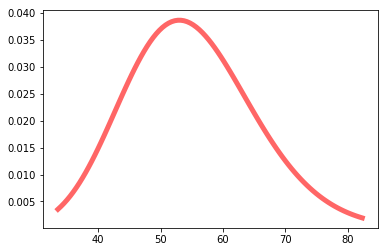
\includegraphics[height=5cm,keepaspectratio=true]{./images/statsChi2.png}
	% statsChi2.png: 0x0 pixel, 300dpi, 0.00x0.00 cm, bb=
	\caption{Función de densidad de distribución $\chi^2$ con $\nu=55$}
	\label{fig:3.9.1}
\end{figure}


\lstinputlisting[language=Python]{../code/chi-cuadrada/statsChi2.py}



\begin{center}
	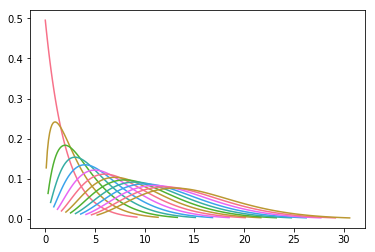
\includegraphics[height=7cm,keepaspectratio=true]{./images/statsChi2Several.png}
	% statsChi2Several.png: 0x0 pixel, 300dpi, 0.00x0.00 cm, bb=
\end{center}


\subsection{Prueba formal de bondad de ajuste}

\begin{teorema}[Prueba $\chi^2$ de bondad de ajuste]
	Sea una muestra clasificada en $k$ categorías mutuamente excluyentes con frecuencias observadas $O_1,\ldots,O_k$ ($\sum_i O_i = N$), y sea $H_0$ la hipótesis de que la población sigue una distribución teórica que asigna probabilidades $p_1,\ldots,p_k$ a dichas categorías. Bajo $H_0$, el estadístico
	\begin{align}
		\chi^2 = \sum_{i=1}^k \frac{(O_i-E_i)^2}{E_i}, \qquad E_i = Np_i,
	\end{align}
	se distribuye asintóticamente como $\chi^2_{\nu}$ con $\nu = k-1-m$ grados de libertad, donde $m\ge 0$ es el número de parámetros del modelo teórico que fueron estimados a partir de la misma muestra (si las probabilidades $p_i$ son completamente conocidas de antemano, $m=0$ y $\nu=k-1$).
\end{teorema}

\begin{observacion}[Regla de Cochran]
	La aproximación $\chi^2$ solo es confiable cuando las frecuencias esperadas no son demasiado pequeñas. La regla práctica de Cochran exige que ninguna $E_i$ sea menor a $1$, y que no más del $20\%$ de las celdas tengan $E_i<5$. Cuando esta condición se viola, la solución estándar es \emph{colapsar o fusionar} categorías adyacentes de baja frecuencia esperada hasta cumplirla, reduciendo correspondientemente los grados de libertad.
\end{observacion}


\section*{Problemas}

\subsection*{Enunciados de los problemas}

% Recordar
\begin{problema}
	\label{prob:3f1ec07}
	Enuncie, sin realizar ningún cálculo, la fórmula del estadístico de bondad de ajuste de Pearson $\chi^2$, y la regla general para determinar sus grados de libertad cuando el modelo teórico está completamente especificado de antemano (sin parámetros estimados de la muestra).
\end{problema}

% Comprender
\begin{problema}
	\label{prob:d4859df}
	Un científico de datos diseña una prueba de bondad de ajuste $\chi^2$ para un modelo de categorización discreta en cuatro clases ($k=4$, $\nu=3$) con $n=80$ observaciones, obteniendo frecuencias esperadas $E_1=45.2$, $E_2=30.5$, $E_3=3.2$, $E_4=1.1$. Explique por qué el cálculo directo del estadístico de Pearson viola las condiciones de regularidad asintótica (la Regla de Cochran), y proponga el procedimiento correctivo estándar, indicando cuántos grados de libertad tendría la prueba ajustada.
\end{problema}

% Aplicar
\begin{problema}
	\label{prob:da2eb15}
	Un genetista indaga si la distribución de grupos sanguíneos ABO en una cohorte sigue las proporciones de referencia nacional: 45\% A, 40\% B, 10\% AB, 5\% O. En una muestra de $n=200$ individuos se observan: A=95, B=75, AB=18, O=12. Realice la prueba de bondad de ajuste al nivel $\alpha=0.05$ (use $\chi^2_{0.05,3}=7.815$).
\end{problema}

% Analizar
\begin{problema}
	\label{prob:d6f0154}
	Un ingeniero registra el conteo diario de interrupciones de un servidor durante $n=100$ días: $0$ interrupciones (36 días), $1$ (40 días), $2$ (18 días), $\ge3$ (6 días, tómese como valor puntual $k=3$). Para verificar si la ocurrencia sigue una Poisson: (a) calcule $\hat\lambda$ por máxima verosimilitud; (b) calcule las frecuencias esperadas bajo Poisson($\hat\lambda$); (c) calcule $\chi^2$ y justifique por qué los grados de libertad correctos son $\nu=k-1-m$ con $m=1$ parámetro estimado. ¿Se acepta el modelo al $\alpha=0.05$?
\end{problema}

% Evaluar
\begin{problema}
	\label{prob:f622374}
	En tablas $2\times2$ con muestras pequeñas o medianas, el estadístico de Pearson $\chi^2$ (sin corrección) tiende a producir p-valores sistemáticamente más bajos que el valor exacto de Fisher, aumentando el riesgo de Error Tipo I. Evalúe por qué ocurre este sesgo, explicando la diferencia entre la naturaleza discreta y escalonada de la distribución hipergeométrica exacta y la naturaleza continua de la $\chi^2_1$ de referencia, y explique cómo la Corrección de Continuidad de Yates ($|ad-bc|-N/2$ en vez de $|ad-bc|$) corrige este sesgo.
\end{problema}

% Crear
\begin{problema}
	\label{prob:369a6a1}
	Diseñe un ejemplo original (contexto, categorías, frecuencias observadas hipotéticas) donde se aplique una prueba de bondad de ajuste $\chi^2$, distinto de los ejemplos de dados, tipos sanguíneos o servidores ya vistos en esta sección. Plantee $H_0$ y $H_a$, calcule las frecuencias esperadas y el estadístico $\chi^2$ para sus datos.
\end{problema}

\subsection*{Soluciones detalladas}

% Recordar
\begin{solproblema}[prob:3f1ec07]
	$\chi^2 = \sum_{i=1}^k \dfrac{(O_i-E_i)^2}{E_i}$. Cuando el modelo está completamente especificado (sin parámetros estimados), los grados de libertad son $\nu=k-1$, donde $k$ es el número de categorías.
\end{solproblema}

% Comprender
\begin{solproblema}[prob:d4859df]
	La aproximación continua de $\chi^2$ a la distribución discreta real de $Q=\sum(O_i-E_i)^2/E_i$ solo es confiable cuando ninguna $E_i$ es menor a $1.0$ y no más del $20\%$ de las celdas tienen $E_i<5$ (Regla de Cochran). Aquí, $E_3=3.2<5$ y $E_4=1.1<5$: el $50\%$ ($2/4$) de las celdas viola la cota, invalidando el uso directo de la tabla $\chi^2$. El procedimiento correctivo estándar es \textbf{agrupar categorías adyacentes de baja frecuencia}: fusionando las clases 3 y 4, $E_{3+4}=3.2+1.1=4.3$, resultando en $k'=3$ categorías efectivas y $\nu_{\text{corregido}}=k'-1=2$ grados de libertad.
\end{solproblema}

% Aplicar
\begin{solproblema}[prob:da2eb15]
	$E_A=90$, $E_B=80$, $E_{AB}=20$, $E_O=10$.
	\begin{align*}
		\chi^2 = \frac{(95-90)^2}{90}+\frac{(75-80)^2}{80}+\frac{(18-20)^2}{20}+\frac{(12-10)^2}{10} = 0.278+0.313+0.200+0.400 = 1.190.
	\end{align*}
	Como $1.190 < 7.815$, \textbf{no se rechaza} $H_0$: la muestra es consistente con las proporciones de referencia nacional.
\end{solproblema}

% Analizar
\begin{solproblema}[prob:d6f0154]
	(a) $\hat\lambda = \bar X = \dfrac{0(36)+1(40)+2(18)+3(6)}{100} = \dfrac{94}{100}=0.94$.
	(b) Con Poisson($0.94$): $E_0\approx39.06$, $E_1\approx36.72$, $E_2\approx17.26$, $E_{\ge3}\approx6.96$.
	(c) $\chi^2 = \dfrac{(36-39.06)^2}{39.06}+\dfrac{(40-36.72)^2}{36.72}+\dfrac{(18-17.26)^2}{17.26}+\dfrac{(6-6.96)^2}{6.96} \approx0.697$. Al estimar $m=1$ parámetro ($\hat\lambda$) de la propia muestra, cada parámetro estimado impone una ligadura adicional sobre las desviaciones $(O_k-E_k)$, reduciendo en una unidad extra la dimensión libre: $\nu=k-1-m=4-1-1=2$. Con $\chi^2_{0.05,2}=5.991$ y $0.697\ll5.991$, \textbf{se acepta} el modelo de Poisson.
\end{solproblema}

% Evaluar
\begin{solproblema}[prob:f622374]
	La distribución teórica exacta de una tabla $2\times2$ finita está dictada por la distribución Hipergeométrica de Fisher, que es \textbf{discreta y escalonada}. La $\chi^2_1$ de referencia, en cambio, es una curva \textbf{continua}. Al aproximar el salto escalonado discreto mediante esa curva continua, el área de la cola derecha (el p-valor) resulta sistemáticamente \textbf{más pequeña} que la probabilidad exacta real, produciendo p-valores artificialmente bajos y un exceso de falsos positivos. La Corrección de Yates ($|ad-bc|-N/2$ en vez de $|ad-bc|$) reduce la magnitud del numerador antes de elevarlo al cuadrado, disminuyendo el valor del estadístico y, por tanto, aumentando el p-valor calculado hacia el valor exacto de Fisher — corrigiendo el sesgo optimista de la aproximación continua sin corrección.
\end{solproblema}

% Crear
\begin{solproblema}[prob:369a6a1]
	\textbf{Ejemplo:} una tienda en línea quiere verificar si las devoluciones de productos se distribuyen uniformemente entre 4 categorías (Ropa, Electrónica, Hogar, Otros) según su política histórica de 40\%, 30\%, 20\%, 10\%. En $n=150$ devoluciones observadas: Ropa=68, Electrónica=40, Hogar=25, Otros=17. $H_0$: las proporciones son 40/30/20/10\%; $H_a$: al menos una difiere. Frecuencias esperadas: $E=[60,45,30,15]$.
	\begin{align*}
		\chi^2 = \frac{(68-60)^2}{60}+\frac{(40-45)^2}{45}+\frac{(25-30)^2}{30}+\frac{(17-15)^2}{15} \approx1.067+0.556+0.833+0.267 = 2.723.
	\end{align*}
	Con $\chi^2_{0.05,3}=7.815$, como $2.723<7.815$, no se rechaza $H_0$.
\end{solproblema}

\section{Pruebas de hipótesis avanzadas: Dos medias, proporciones, varianzas y homogeneidad}

En las secciones precedentes de este capítulo sentamos las bases filosóficas y procedimentales de la docimasia estadística: formulamos la hipótesis nula ($H_0$) y alternativa ($H_a$), analizamos los errores de Tipo I ($\alpha$) y Tipo II ($\beta$), y estudiamos las pruebas clásicas $Z$ y $t$ para una sola media. Asimismo, introdujimos la prueba $\chi^2$ para verificar la bondad de ajuste de una distribución y para contrastar la independencia entre dos variables categóricas en una misma población.

En la práctica empírica de la ciencia de datos, la analítica experimental y el diseño industrial, el investigador se enfrenta continuamente a preguntas comparativas y multidimensionales: ¿Es el algoritmo $A$ significativamente más rápido que el algoritmo $B$? ¿Difiere la tasa de clics o conversión en tres segmentos demográficos distintos? ¿La introducción de un nuevo sensor aumenta la estabilidad (reduce la varianza) del sistema?

En esta sección desarrollamos de manera completa y rigurosa la teoría y metodología para contrastar hipótesis relativas a dos medias, una y dos proporciones, una y dos varianzas, así como las pruebas de homogeneidad y comparación simultánea de múltiples proporciones.

\subsection{Pruebas de hipótesis sobre dos medias ($\mu_1 - \mu_2$)}

Al comparar las medias poblacionales de dos grupos ($\mu_1$ y $\mu_2$), contrastamos una hipótesis nula de la forma:
\begin{align}
	H_0: \mu_1 - \mu_2 = \Delta_0,
\end{align}
donde $\Delta_0$ es la diferencia hipotética (en la gran mayoría de las investigaciones comparativas se postula que no existe diferencia inicial, es decir, $\Delta_0 = 0 \implies \mu_1 = \mu_2$).

La hipótesis alternativa ($H_a$) puede adoptar tres formas, determinando la estructura de la región de rechazo:
\begin{itemize}
	\item \textbf{Prueba de dos colas:} $H_a: \mu_1 - \mu_2 \neq \Delta_0$.
	\item \textbf{Prueba de cola izquierda:} $H_a: \mu_1 - \mu_2 < \Delta_0$.
	\item \textbf{Prueba de cola derecha:} $H_a: \mu_1 - \mu_2 > \Delta_0$.
\end{itemize}

El estadístico de prueba a emplear depende de si las varianzas poblacionales son conocidas o desconocidas y de si las muestras son independientes o pareadas.

\begin{teorema}[Caso 1: Muestras independientes con varianzas poblacionales conocidas]
	Sean dos muestras aleatorias independientes de tamaños $n_1$ y $n_2$ provenientes de poblaciones normales con medias $\mu_1, \mu_2$ y varianzas conocidas $\sigma_1^2, \sigma_2^2$. (Si $n_1, n_2 \geq 30$, la normalidad poblacional no es estrictamente necesaria por el Teorema del Límite Central). Bajo la hipótesis nula $H_0: \mu_1 - \mu_2 = \Delta_0$, el estadístico estandarizado:
	\begin{align}
		Z = \frac{(\bar{X}_1 - \bar{X}_2) - \Delta_0}{\sqrt{\frac{\sigma_1^2}{n_1} + \frac{\sigma_2^2}{n_2}}}
	\end{align}
	sigue exactamente una distribución normal estándar $N(0,1)$. Rechazamos $H_0$ al nivel de significancia $\alpha$ si $|Z| > Z_{\alpha/2}$ (dos colas), $Z < -Z_\alpha$ (cola izquierda) o $Z > Z_\alpha$ (cola derecha).
\end{teorema}

\begin{teorema}[Caso 2: Muestras independientes con varianzas desconocidas pero iguales (Homoscedasticidad)]
	Cuando $\sigma_1^2, \sigma_2^2$ son desconocidas pero se puede asumir razonablemente que son iguales ($\sigma_1^2 = \sigma_2^2 = \sigma^2$), estimamos la varianza común mediante la varianza muestral combinada $S_p^2$:
	\begin{align}
		S_p^2 = \frac{(n_1 - 1)S_1^2 + (n_2 - 1)S_2^2}{n_1 + n_2 - 2}.
	\end{align}
	El estadístico de prueba bajo $H_0: \mu_1 - \mu_2 = \Delta_0$ es:
	\begin{align}
		t = \frac{(\bar{X}_1 - \bar{X}_2) - \Delta_0}{S_p \sqrt{\frac{1}{n_1} + \frac{1}{n_2}}},
	\end{align}
	el cual sigue una distribución $t$ de Student con $\nu = n_1 + n_2 - 2$ grados de libertad.
\end{teorema}

\begin{teorema}[Caso 3: Muestras independientes con varianzas desconocidas y diferentes (Welch)]
	Si las varianzas poblacionales son desconocidas y notablemente distintas ($\sigma_1^2 \neq \sigma_2^2$), no podemos combinar las varianzas muestrales. El estadístico de prueba es:
	\begin{align}
		t = \frac{(\bar{X}_1 - \bar{X}_2) - \Delta_0}{\sqrt{\frac{S_1^2}{n_1} + \frac{S_2^2}{n_2}}},
	\end{align}
	cuya distribución muestral se aproxima de manera excelente mediante la distribución $t$ de Student con los grados de libertad de Welch-Satterthwaite:
	\begin{align}
		\nu = \frac{\left( \frac{S_1^2}{n_1} + \frac{S_2^2}{n_2} \right)^2}{\frac{\left(S_1^2/n_1\right)^2}{n_1 - 1} + \frac{\left(S_2^2/n_2\right)^2}{n_2 - 1}}.
	\end{align}
\end{teorema}

\begin{definicion}[Caso 4: Muestras pareadas o dependientes]
	Cuando las mediciones de los dos grupos se realizan sobre los mismos sujetos o unidades experimentales apareadas ($X_{1i}, X_{2i}$), se define la variable diferencia $D_i = X_{1i} - X_{2i}$. El contraste sobre $\mu_1 - \mu_2$ se transforma en una prueba $t$ de una sola muestra sobre la media de las diferencias $\mu_D$. Bajo $H_0: \mu_D = \Delta_0$:
	\begin{align}
		t = \frac{\bar{D} - \Delta_0}{S_D / \sqrt{n}},
	\end{align}
	donde $\bar{D} = \frac{1}{n}\sum D_i$ y $S_D = \sqrt{\frac{1}{n-1}\sum (D_i - \bar{D})^2}$. El estadístico sigue una distribución $t$ de Student con $\nu = n - 1$ grados de libertad.
\end{definicion}

\subsection{Pruebas relacionadas con proporciones}

En el modelado estadístico y aprendizaje automático, evaluar variables categóricas o binarias (éxito/fracaso) requiere contrastar proporciones poblacionales.

\begin{teorema}[Prueba $Z$ para una proporción poblacional]
	Sea $X$ el número de éxitos en una muestra aleatoria de tamaño $n$ de una distribución binomial con probabilidad real $p$. Para contrastar la hipótesis nula $H_0: p = p_0$ cuando el tamaño muestral cumple las condiciones de aproximación normal ($n p_0 \geq 5$ y $n(1-p_0) \geq 5$), el estadístico de prueba estandarizado es:
	\begin{align}
		Z = \frac{\hat{p} - p_0}{\sqrt{\frac{p_0(1-p_0)}{n}}},
	\end{align}
	donde $\hat{p} = X/n$ es la proporción observada. Notemos una diferencia teórica crucial respecto al intervalo de confianza: en el denominador del estadístico $Z$ se utiliza la desviación estándar esperada \emph{bajo la hipótesis nula} ($p_0(1-p_0)$), no la varianza muestral empírica ($\hat{p}(1-\hat{p})$).
\end{teorema}

\begin{teorema}[Prueba $Z$ para la diferencia de dos proporciones]
	Para comparar las tasas de éxito de dos poblaciones independientes ($p_1$ y $p_2$), contrastamos la hipótesis nula de igualdad $H_0: p_1 - p_2 = 0$ ($p_1 = p_2 = p$).
	
	Dado que bajo la hipótesis nula ambas muestras proceden teóricamente de una misma población que comparte la proporción común $p$, el estimador puntual más eficiente de dicha proporción es el promedio ponderado de éxitos de ambas muestras, conocido como \emph{proporción combinada o agrupada} ($\bar{p}$):
	\begin{align}
		\bar{p} = \frac{X_1 + X_2}{n_1 + n_2} = \frac{n_1 \hat{p}_1 + n_2 \hat{p}_2}{n_1 + n_2}.
		\label{eq:prop_combinada}
	\end{align}
	
	El estadístico de prueba bajo $H_0$ es:
	\begin{align}
		Z = \frac{\hat{p}_1 - \hat{p}_2}{\sqrt{\bar{p}(1-\bar{p})\left(\frac{1}{n_1} + \frac{1}{n_2}\right)}},
	\end{align}
	el cual se distribuye asintóticamente como una normal estándar $N(0,1)$ cuando $n_1 \bar{p}, n_1(1-\bar{p}), n_2 \bar{p}, n_2(1-\bar{p}) \geq 5$.
\end{teorema}

\subsection{Pruebas relacionadas con varianzas}

La docimasia de varianzas y dispersiones es indispensable no solo para evaluar uniformidad o riesgo, sino para validar los supuestos de homoscedasticidad en modelos paramétricos.

\begin{teorema}[Prueba $\chi^2$ para la varianza de una población normal]
	Para contrastar si la varianza de una población normal es igual a un valor hipotético $H_0: \sigma^2 = \sigma_0^2$, calculamos la varianza muestral $S^2$ de una muestra de tamaño $n$. El estadístico de prueba es:
	\begin{align}
		\chi^2 = \frac{(n-1)S^2}{\sigma_0^2}.
	\end{align}
	Bajo $H_0$, este estadístico sigue una distribución chi-cuadrada con $\nu = n - 1$ grados de libertad.
	Para una prueba de dos colas ($H_a: \sigma^2 \neq \sigma_0^2$), rechazamos $H_0$ al nivel $\alpha$ si $\chi^2 < \chi^2_{1-\alpha/2, n-1}$ o si $\chi^2 > \chi^2_{\alpha/2, n-1}$.
\end{teorema}

\begin{teorema}[Prueba $F$ para la comparación de dos varianzas poblacionales]
	Para contrastar la hipótesis de igualdad de varianzas entre dos poblaciones normales independientes ($H_0: \sigma_1^2 = \sigma_2^2$), extraemos muestras de tamaños $n_1$ y $n_2$ y calculamos sus varianzas $S_1^2$ y $S_2^2$. El estadístico de prueba es el cociente de las varianzas muestrales:
	\begin{align}
		F = \frac{S_1^2}{S_2^2}.
	\end{align}
	Bajo $H_0$, este estadístico sigue una distribución $F$ de Snedecor con $\nu_1 = n_1 - 1$ grados de libertad en el numerador y $\nu_2 = n_2 - 1$ en el denominador.
	Para una prueba de dos colas ($H_a: \sigma_1^2 \neq \sigma_2^2$), se rechaza $H_0$ si $F > F_{\alpha/2, \nu_1, \nu_2}$ o si $F < F_{1-\alpha/2, \nu_1, \nu_2} = \frac{1}{F_{\alpha/2, \nu_2, \nu_1}}$.
\end{teorema}

\subsection{Pruebas de homogeneidad vs Pruebas de independencia}

En la sección \ref{sec:3.9} exploramos la aplicación de la distribución chi-cuadrada en tablas de contingencia para evaluar la \emph{independencia} entre dos factores. Existe otra prueba de capital importancia para la comparación multidimensional: la \emph{prueba de homogeneidad}. Aunque la fórmula matemática de cálculo ($\sum \frac{(O-E)^2}{E}$) es exactamente la misma en ambos casos, existe una diferencia conceptual profunda en el diseño experimental y el muestreo.

\begin{definicion}[Diferencia conceptual entre Independencia y Homogeneidad]
	\begin{itemize}
		\item \textbf{Prueba de Independencia:} Se extrae \textbf{una sola muestra aleatoria} de tamaño total $N$ de una única población y, a posteriori, se clasifica cruzadamente cada observación según dos variables categóricas $A$ (con $r$ niveles) y $B$ (con $c$ niveles). Ningún total marginal de fila o columna está fijado de antemano por el investigador (salvo el total general $N$). La hipótesis contrastada es $H_0: P(A_i \cap B_j) = P(A_i)P(B_j)$.
		\item \textbf{Prueba de Homogeneidad:} Se extraen \textbf{$c$ muestras aleatorias independientes} de tamaños preestablecidos ($n_1, n_2, \ldots, n_c$, fijando los totales de columna por el diseño experimental) procedentes de $c$ subgrupos o poblaciones distintas. Para cada subgrupo, se mide la distribución de \textbf{una única variable categórica} con $r$ niveles. La hipótesis contrastada es que las $c$ poblaciones poseen idéntica distribución categórica:
		\begin{align}
			H_0: p_{i1} = p_{i2} = \ldots = p_{ic} \quad \text{para cada categoría } i = 1, 2, \ldots, r,
		\end{align}
		donde $p_{ij}$ es la probabilidad de que una observación del subgrupo $j$ caiga en la categoría $i$.
	\end{itemize}
\end{definicion}

\begin{teorema}[Estadístico chi-cuadrada para homogeneidad]
	Dada una tabla de datos de $r$ filas (categorías) y $c$ columnas (poblaciones o subgrupos independientes), si $O_{ij}$ es la frecuencia observada en la celda $(i,j)$, la frecuencia esperada bajo la hipótesis nula de homogeneidad es:
	\begin{align}
		E_{ij} = \frac{R_i \cdot C_j}{N},
	\end{align}
	donde $R_i = \sum_{j=1}^c O_{ij}$ es el total de la fila $i$, $C_j = n_j = \sum_{i=1}^r O_{ij}$ es el tamaño de la muestra de la población $j$, y $N = \sum C_j$ es el total general.
	
	El estadístico de prueba:
	\begin{align}
		\chi^2 = \sum_{i=1}^r \sum_{j=1}^c \frac{(O_{ij} - E_{ij})^2}{E_{ij}}
	\end{align}
	se distribuye asintóticamente (cuando todos los $E_{ij} \geq 5$) como una chi-cuadrada con $\nu = (r-1)(c-1)$ grados de libertad.
\end{teorema}

\subsection{Pruebas de varias proporciones y procedimiento de Marascuilo}

La comparación de varias proporciones binomiales es un caso especial de gran relevancia técnica de la prueba de homogeneidad, donde la variable dependiente es dicotómica ($r=2$: Éxito vs Fracaso) y evaluamos $c = k$ poblaciones independientes.

\begin{definicion}[Contraste de $k$ proporciones]
	Sean $p_1, p_2, \ldots, p_k$ las proporciones verdaderas de éxito en $k$ poblaciones independientes. La hipótesis nula es:
	\begin{align}
		H_0: p_1 = p_2 = \ldots = p_k = p,
	\end{align}
	frente a la hipótesis alternativa $H_a$: al menos una de las proporciones difiere de las demás.
	
	El estadístico $\chi^2$ de homogeneidad aplicado a la tabla $2 \times k$ tiene $\nu = (2-1)(k-1) = k-1$ grados de libertad. Puede demostrarse algebraicamente que el estadístico se expresa de forma compacta como:
	\begin{align}
		\chi^2 = \sum_{j=1}^k \frac{(X_j - n_j \bar{p})^2}{n_j \bar{p}(1-\bar{p})},
		\label{eq:chi2_k_prop}
	\end{align}
	donde $X_j$ es el número de éxitos en la muestra $j$ (de tamaño $n_j$), y $\bar{p} = \frac{\sum X_j}{\sum n_j}$ es la proporción global de éxitos en las $k$ muestras.
\end{definicion}

Cuando el estadístico $\chi^2$ es significativo y rechazamos $H_0$, sabemos con certeza estadística que las $k$ proporciones no son todas iguales, pero la prueba global no nos dice \emph{cuáles} específicas difieren entre sí. Para identificar los pares significativos sin cometer el error de inflar la probabilidad de error Tipo I global al realizar $\binom{k}{2}$ pruebas individuales de diferencia de proporciones, utilizamos el procedimiento de comparación múltiple de Marascuilo.

\begin{teorema}[Procedimiento de comparación post-hoc de Marascuilo]
	Si la prueba global $\chi^2$ de $k$ proporciones rechaza $H_0$ al nivel de significancia $\alpha$, las diferencias absolutas observadas entre cada par de proporciones muestrales ($|\hat{p}_i - \hat{p}_j|$ para todo $1 \leq i < j \leq k$) se comparan contra un rango crítico par a par $r_{ij}$ dado por:
	\begin{align}
		r_{ij} = \sqrt{\chi^2_{\alpha, \, k-1}} \sqrt{\frac{\hat{p}_i(1-\hat{p}_i)}{n_i} + \frac{\hat{p}_j(1-\hat{p}_j)}{n_j}},
		\label{eq:marascuilo}
	\end{align}
	donde $\chi^2_{\alpha, k-1}$ es el valor crítico superior del estadístico global con $k-1$ grados de libertad. 
	
	Declaramos que las proporciones poblacionales $p_i$ y $p_j$ difieren significativamente al nivel familiar de error $\alpha$ si y solo si $|\hat{p}_i - \hat{p}_j| > r_{ij}$.
\end{teorema}

\section{Problemas resueltos de docimasia avanzada}

\subsection{Enunciados de los problemas}

\subsubsection*{1. Nivel Fundamental (Sencillos / Directos)}

\begin{problema}
	\label{prob:doc_dos_medias_iguales}
	Una empresa de telemedicina evalúa si el tiempo medio de respuesta en consultas de medicina general difiere entre dos plataformas digitales (Plataforma 1 vs. Plataforma 2). Se obtienen dos muestras aleatorias independientes de tiempos (en minutos):
	\begin{itemize}
		\item \textbf{Plataforma 1:} $n_1 = 16$, $\bar{X}_1 = 14.2$ min, $S_1 = 2.4$ min.
		\item \textbf{Plataforma 2:} $n_2 = 18$, $\bar{X}_2 = 16.8$ min, $S_2 = 2.6$ min.
	\end{itemize}
	Asumiendo que las poblaciones son normales y las varianzas son iguales ($\sigma_1^2 = \sigma_2^2$), realice una prueba de hipótesis al nivel de significancia del $5\%$ ($\alpha = 0.05$) para determinar si existe una diferencia real en los tiempos medios de respuesta.
\end{problema}

\begin{problema}
	\label{prob:doc_pareadas}
	En una investigación sobre el rendimiento físico de deportistas tras someterse a un programa de entrenamiento en altitud, se midió el consumo máximo de oxígeno ($\text{VO}_2$ máx en ml/kg/min) en una muestra de $n = 12$ atletas \emph{antes} ($X_1$) y \emph{después} ($X_2$) del programa de 8 semanas. Las diferencias individuales $D_i = X_{2i} - X_{1i}$ arrojaron una media muestral de incremento $\bar{D} = 3.8$ ml/kg/min y una desviación estándar de las diferencias $S_D = 2.1$ ml/kg/min.
	
	¿Aportan los datos evidencia suficiente al nivel $\alpha = 0.01$ para afirmar que el programa de entrenamiento en altitud \textbf{aumenta} significativamente el consumo máximo de oxígeno?
\end{problema}

\begin{problema}
	\label{prob:doc_dos_proporciones}
	Una compañía de ciberseguridad compara la efectividad del filtro antispam clásico frente a un nuevo modelo con inteligencia artificial basada en transformadores. Al procesar dos muestras independientes de correos electrónicos entrantes verificados:
	\begin{itemize}
		\item \textbf{Filtro Clásico:} Se detectaron correctamente como spam $X_1 = 340$ de $n_1 = 400$ correos maliciosos.
		\item \textbf{Modelo IA:} Se detectaron correctamente como spam $X_2 = 465$ de $n_2 = 500$ correos maliciosos.
	\end{itemize}
	¿Existe evidencia al nivel $\alpha = 0.02$ para afirmar que el Modelo de IA tiene una \textbf{tasa de detección significativamente superior} a la del Filtro Clásico?
\end{problema}

\subsubsection*{2. Nivel Operativo (Intermedios / De Desarrollo)}

\begin{problema}
	\label{prob:doc_dos_varianzas}
	Antes de realizar una prueba $t$ agrupada de comparación de medias de dos sensores analógicos, se debe comprobar si se cumple el supuesto de homoscedasticidad ($H_0: \sigma_1^2 = \sigma_2^2$). Se toman dos muestras aleatorias independientes con varianzas muestrales $S_1^2 = 14.8$ ($n_1 = 16$) y $S_2^2 = 5.2$ ($n_2 = 11$).
	
	Realice una prueba $F$ de dos colas al nivel $\alpha = 0.10$ para contrastar la hipótesis de igualdad de varianzas. ¿Es legítimo asumir homoscedasticidad?
\end{problema}

\begin{problema}
	\label{prob:homogeneidad_contingencia}
	Una firma de investigación de mercados analiza las preferencias de tres cohortes generacionales de usuarios de software (Generación Z, Millennials y Generación X) respecto al modelo de monetización preferido en herramientas digitales: Subscripción mensual, Pago único (licencia perpetua) o Freemium con publicidad. Se seleccionan tres muestras independientes de tamaños fijos $n_1 = 200$, $n_2 = 250$ y $n_3 = 150$, obteniéndose las frecuencias observadas en la Tabla \ref{tab:homog_obs}.
	\begin{table}[h!]
		\centering
		\begin{tabular}{lcccc}
			\hline
			\textbf{Modelo Preferido} & \textbf{Gen Z ($j=1$)} & \textbf{Millennials ($j=2$)} & \textbf{Gen X ($j=3$)} & \textbf{Total Fila ($R_i$)} \\ \hline
			Subscripción ($i=1$) & 80 & 120 & 45 & \textbf{245} \\
			Pago Único ($i=2$) & 30 & 65 & 70 & \textbf{165} \\
			Freemium ($i=3$) & 90 & 65 & 35 & \textbf{190} \\ \hline
			\textbf{Total Columna ($C_j$)} & \textbf{200} & \textbf{250} & \textbf{150} & \textbf{600} \\ \hline
		\end{tabular}
		\caption{Frecuencias observadas ($O_{ij}$) por modelo de monetización en tres cohortes generacionales.}
		\label{tab:homog_obs}
	\end{table}
	
	Realice una prueba de homogeneidad de proporciones al nivel $\alpha = 0.01$ para determinar si la distribución de preferencias de monetización es idéntica en las tres generaciones.
\end{problema}

\begin{problema}
	\label{prob:doc_welch_hetero}
	Un científico de datos compara los tiempos de ejecución intermedios (en segundos) que consumen dos algoritmos de clústeres dispersos. Dado que la arquitectura de hardware del segundo algoritmo genera mucha más volatilidad, las varianzas poblacionales son explícitamente heterogéneas ($\sigma_1^2 \neq \sigma_2^2$). Se extraen las siguientes mediciones experimentales:
	\begin{itemize}
		\item \textbf{Algoritmo 1:} $n_1 = 15$, $\bar{X}_1 = 85.2$ s, $S_1 = 12.4$ s.
		\item \textbf{Algoritmo 2:} $n_2 = 18$, $\bar{X}_2 = 74.5$ s, $S_2 = 5.2$ s.
	\end{itemize}
	\begin{enumerate}
		\item Calcule los grados de libertad efectivos ($\nu$) mediante la ecuación de Welch-Satterthwaite.
		\item Ejecute la prueba $t$ de Welch bilateral con $\alpha = 0.05$ para determinar si los tiempos medios de ejecución de ambos algoritmos difieren de manera estadísticamente significativa.
	\end{enumerate}
\end{problema}

\subsubsection*{3. Nivel Analítico (Avanzados / De Conexión)}

\begin{problema}
	\label{prob:doc_k_proporciones_marascuilo}
	Para evaluar el nivel de adherencia a estándares éticos sobre sesgo algorítmico, una entidad fiscalizadora examina muestras de modelos de aprendizaje automático desplegados por $k = 4$ empresas corporativas de tecnología (Empresas A, B, C y D). Se verifica si el modelo cumple con los criterios de imparcialidad (Éxito = Cumple, Fracaso = No cumple):
	\begin{itemize}
		\item \textbf{Empresa A:} $X_1 = 82$ cumplen, de $n_1 = 100$ modelos ($\hat{p}_1 = 0.820$).
		\item \textbf{Empresa B:} $X_2 = 64$ cumplen, de $n_2 = 100$ modelos ($\hat{p}_2 = 0.640$).
		\item \textbf{Empresa C:} $X_3 = 90$ cumplen, de $n_3 = 120$ modelos ($\hat{p}_3 = 0.750$).
		\item \textbf{Empresa D:} $X_4 = 44$ cumplen, de $n_4 = 80$ modelos ($\hat{p}_4 = 0.550$).
	\end{itemize}
	\begin{enumerate}
		\item Realice una prueba global $\chi^2$ de igualdad de proporciones ($H_0: p_1=p_2=p_3=p_4$) al nivel $\alpha = 0.05$.
		\item Si se rechaza la hipótesis nula global, aplique el \textbf{procedimiento de comparación post-hoc de Marascuilo} para determinar cuáles parejas de empresas difieren significativamente entre sí al nivel familiar de $\alpha = 0.05$.
	\end{enumerate}
\end{problema}

\begin{problema}
	\label{prob:doc_errores_potencia_muestra}
	\textbf{Análisis integral del Error Tipo I ($\alpha$), Error Tipo II ($\beta$) y Potencia estadística ($1-\beta$):}
	El tiempo de respuesta del servidor de procesamiento de transacciones de una fintech sigue una distribución normal con desviación estándar poblacional conocida $\sigma = 15$ milisegundos. El estándar operativo exige que la latencia media no supere los $100$ ms ($H_0: \mu \le 100$ vs. $H_a: \mu > 100$). Se monitorea una muestra aleatoria diaria de $n = 25$ transacciones con un nivel de significancia $\alpha = 0.05$.
	\begin{enumerate}
		\item Determine la regla de decisión en la escala original del promedio muestral de latencia ($\bar{X}_c = \mu_0 + Z_\alpha \frac{\sigma}{\sqrt{n}}$).
		\item Suponga que debido a una sobrecarga en la red, la latencia media real de la población aumentó silenciosamente a $\mu_a = 108$ ms. Calcule la probabilidad exacta de cometer un \textbf{Error Tipo II ($\beta$)} —no detectar la sobrecarga— y determine el valor exacto de la \textbf{Potencia de la prueba ($1-\beta$)}.
		\item Si el director de ingeniería exige que la prueba mantenga un riesgo $\alpha = 0.05$ pero sea capaz de detectar una sobrecarga real de $\mu_a = 108$ ms con una \textbf{Potencia estadística del $90\%$} ($1-\beta = 0.90 \implies Z_\beta = 1.282$), deduzca y calcule exactamente qué tamaño de muestra $n$ debe procesar el sistema en cada auditoría.
	\end{enumerate}
\end{problema}

\subsubsection*{4. Nivel Desafiante (Expertos / Deducción Profunda)}

\begin{problema}
	\label{prob:doc_desaf_lrt_wilks}
	\textbf{Deducción de la Prueba de Razón de Verosimilitudes (\emph{Likelihood Ratio Test}, LRT) para varianzas e invocación del Teorema de Wilks:}
	Sean dos muestras aleatorias independientes $X_1, \dots, X_{n_1} \sim N(\mu_1, \sigma_1^2)$ y $Y_1, \dots, Y_{n_2} \sim N(\mu_2, \sigma_2^2)$ donde tanto las medias como las varianzas son completamente desconocidas. Se desea docimar la hipótesis paramétrica de homoscedasticidad $H_0: \sigma_1^2 = \sigma_2^2 = \sigma^2$ frente a $H_a: \sigma_1^2 \neq \sigma_2^2$.
	\begin{enumerate}
		\item Deduzca el logaritmo de la función de verosimilitud bivariada conjunta $\ln L(\mu_1, \mu_2, \sigma_1^2, \sigma_2^2)$ bajo el espacio paramétrico total sin restricciones $\Theta$, explicitando los estimadores máximo verosímiles de dispersión $\hat{\sigma}_1^2 = \frac{1}{n_1}\sum (X_i - \bar{X})^2$ y $\hat{\sigma}_2^2 = \frac{1}{n_2}\sum (Y_i - \bar{Y})^2$.
		\item Deduzca el logaritmo de la verosimilitud bajo el subespacio nulo restringido $\Theta_0$ (donde $\sigma_1^2 = \sigma_2^2 = \sigma_0^2$), demostrando que la estimación combinada de máxima verosimilitud es:
		\begin{align}
			\hat{\sigma}_0^2 = \frac{n_1 \hat{\sigma}_1^2 + n_2 \hat{\sigma}_2^2}{n_1 + n_2}.
		\end{align}
		\item Demuestre que el estadístico logarítmico de la razón de verosimilitudes $\Lambda = \dfrac{L(\Theta_0)}{L(\Theta)}$ cumple la identidad algebraica exacta:
		\begin{align}
			-2 \ln \Lambda = n_1 \ln\left( \frac{\hat{\sigma}_0^2}{\hat{\sigma}_1^2} \right) + n_2 \ln\left( \frac{\hat{\sigma}_0^2}{\hat{\sigma}_2^2} \right).
		\end{align}
		\item Explique por qué, bajo la hipótesis nula, la distribución en el muestreo de $-2 \ln \Lambda$ converge asintóticamente al orden de $\chi^2_1$ según el \textbf{Teorema de Samuel S. Wilks}, argumentando el cómputo de la dimensión paramétrica perdida entre $\Theta$ y $\Theta_0$.
	\end{enumerate}
\end{problema}

\begin{problema}
	\label{prob:doc_desaf_pvalor_teorema}
	\textbf{Estructura probabilística, dominancia estocástica y geometría analítica del Valor-$p$:}
	En la literatura de ciencia de datos es habitual confundir el valor-$p$ observado con la probabilidad posterior de la hipótesis nula ($P(H_0 \mid \text{datos})$). Formalice la verdadera naturaleza del valor-$p$ considerándolo una variable aleatoria $P(X)$ sobre el espacio de las muestras observadas:
	\begin{enumerate}
		\item Sea una prueba univariada continua cuyo estadístico docimásica $T(X)$ posee una función de distribución estrictamente monótona continua $F_0(t) = P_{H_0}(T \le t)$ y función de supervivencia $S_0(t) = 1 - F_0(t) = P_{H_0}(T \ge t)$ bajo la hipótesis nula. El valor-$p$ aleatorio para pruebas de cola superior se define por $P = S_0(T)$.
		Demuestre con rigor mediante la diferenciación y el Teorema de la Transformada de Probabilidad Integral (\emph{Probability Integral Transform}) que, \textbf{cuando $H_0$ es verdadera, la variable aleatoria p-valor $P$ se distribuye en forma exactamente Uniforme sobre el intervalo unitario $[0, 1]$} ($P \sim U(0,1)$), cumpliendo $P_{H_0}(P \le \alpha) = \alpha$ para todo $\alpha \in (0,1)$.
		\item Cuando la hipótesis alternativa $H_a$ es verdadera (existe un tamaño de efecto real en la naturaleza), el estadístico adopta una distribución alternativa diferente $F_a(t) = P_{H_a}(T \le t)$. Demuestre algebraicamente que la función de distribución acumulada del p-valor bajo $H_a$, denotada por $G_P(u) = P_{H_a}(P \le u)$ para $u \in (0,1)$, es una función \textbf{estrictamente cóncava} que domina estocásticamente a la diagonal uniforme ($G_P(u) > u$).
		\item Demuestre por qué la densidad diferencial del p-valor en el límite del rechazo absoluto $\lim_{u \to 0^+} g_P(u) = \lim_{u \to 0^+} G_P'(u)$ es directamente proporcional al \textbf{cociente de verosimilitudes monótono} $\dfrac{f_a(t)}{f_0(t)}$ en la región extrema $t \to \infty$, justificando por qué ante cualquier efecto real los p-valores experimentales se aglomeran masivamente en la vecindad inmediata del cero.
	\end{enumerate}
\end{problema}


\subsection{Soluciones detalladas}

\subsubsection*{1. Nivel Fundamental (Sencillos / Directos)}

\begin{solproblema}
	\textbf{Paso 1: Planteamiento de hipótesis.}
	Queremos contrastar la igualdad de ambas medias contra una diferencia bidireccional:
	\begin{align}
		H_0&: \mu_1 - \mu_2 = 0 \\
		H_a&: \mu_1 - \mu_2 \neq 0
	\end{align}
	
	\textbf{Paso 2: Cálculo de la varianza combinada ($S_p^2$).}
	Los grados de libertad son $\nu = n_1 + n_2 - 2 = 16 + 18 - 2 = 32$.
	\begin{align}
		S_p^2 &= \frac{(n_1 - 1)S_1^2 + (n_2 - 1)S_2^2}{n_1 + n_2 - 2} = \frac{(15)(2.4)^2 + (17)(2.6)^2}{32} \\
		&= \frac{15(5.76) + 17(6.76)}{32} = \frac{86.4 + 114.92}{32} = \frac{201.32}{32} \approx 6.29125 \text{ min}^2.
	\end{align}
	La desviación estándar agrupada es $S_p = \sqrt{6.29125} \approx 2.508$ min.
	
	\textbf{Paso 3: Cálculo del estadístico $t$ de prueba.}
	\begin{align}
		t = \frac{(\bar{X}_1 - \bar{X}_2) - 0}{S_p \sqrt{\frac{1}{n_1} + \frac{1}{n_2}}} = \frac{14.2 - 16.8}{2.508 \sqrt{\frac{1}{16} + \frac{1}{18}}} = \frac{-2.6}{2.508 \sqrt{0.0625 + 0.05556}} = \frac{-2.6}{2.508 \times 0.3436} \approx \frac{-2.6}{0.8617} \approx -3.017.
	\end{align}
	
	\textbf{Paso 4: Regla de decisión y conclusión.}
	Para una prueba de dos colas con $\alpha = 0.05$ y $\nu = 32$ grados de libertad, el valor crítico en la tabla $t$ es $t_{0.025, \, 32} \approx 2.037$.
	La región de rechazo está formada por los valores $t < -2.037$ o $t > 2.037$.
	
	Como el estadístico calculado $t = -3.017$ cae claramente en la región de rechazo de la cola izquierda ($-3.017 < -2.037$), \textbf{rechazamos $H_0$}. Concluimos al nivel del $5\%$ que existe una diferencia estadísticamente significativa en los tiempos medios de respuesta entre ambas plataformas, siendo la Plataforma 1 significativamente más rápida.
\end{solproblema}

\begin{solproblema}
	\textbf{Paso 1: Planteamiento de hipótesis de una cola (pareadas).}
	Como evaluamos si el programa incrementa el valor después respecto al valor antes ($X_2 > X_1 \implies D > 0$), formulamos una prueba de cola derecha sobre la media poblacional de las diferencias $\mu_D$:
	\begin{align}
		H_0&: \mu_D \leq 0 \\
		H_a&: \mu_D > 0
	\end{align}
	
	\textbf{Paso 2: Cálculo del estadístico $t$ para muestras pareadas.}
	Los grados de libertad son $\nu = n - 1 = 12 - 1 = 11$.
	\begin{align}
		t = \frac{\bar{D} - 0}{S_D / \sqrt{n}} = \frac{3.8}{2.1 / \sqrt{12}} = \frac{3.8}{2.1 / 3.4641} = \frac{3.8}{0.6062} \approx 6.268.
	\end{align}
	
	\textbf{Paso 3: Regla de decisión y conclusión.}
	Para una prueba unilateral superior con $\alpha = 0.01$ y $\nu = 11$, el valor crítico de la distribución $t$ de Student es:
	\begin{align}
		t_{0.01, \, 11} = 2.718.
	\end{align}
	La región de rechazo es $t > 2.718$. Dado que nuestro valor observado $t = 6.268 \gg 2.718$, \textbf{rechazamos categóricamente $H_0$}. Existe evidencia estadística abrumadora al nivel del $1\%$ para afirmar que el programa de entrenamiento en altitud produce un incremento real en el $\text{VO}_2$ máximo de los atletas.
\end{solproblema}

\begin{solproblema}
	\textbf{Paso 1: Planteamiento de hipótesis.}
	Denotemos por $p_1$ y $p_2$ las proporciones de detección poblacional del filtro clásico y del modelo IA, respectivamente. Evaluamos si $p_2 > p_1$, es decir, si $p_1 - p_2 < 0$:
	\begin{align}
		H_0&: p_1 - p_2 \geq 0 \\
		H_a&: p_1 - p_2 < 0 \quad \text{(prueba de cola izquierda)}.
	\end{align}
	
	\textbf{Paso 2: Proporciones empíricas y proporción combinada ($\bar{p}$).}
	Las proporciones individuales son $\hat{p}_1 = 340/400 = 0.850$ ($85\%$) y $\hat{p}_2 = 465/500 = 0.930$ ($93\%$).
	Bajo la hipótesis nula de que ambas proporciones son iguales, el estimador agrupado combinando ambas muestras es:
	\begin{align}
		\bar{p} = \frac{X_1 + X_2}{n_1 + n_2} = \frac{340 + 465}{400 + 500} = \frac{805}{900} \approx 0.89444.
	\end{align}
	
	\textbf{Paso 3: Cálculo del estadístico $Z$ de prueba.}
	El error estándar bajo $H_0$ es:
	\begin{align}
		SE_0 = \sqrt{\bar{p}(1-\bar{p})\left(\frac{1}{n_1} + \frac{1}{n_2}\right)} &= \sqrt{0.89444(0.10556)\left(\frac{1}{400} + \frac{1}{500}\right)} \\
		&= \sqrt{0.094416 \times 0.0045} = \sqrt{0.00042487} \approx 0.02061.
	\end{align}
	El estadístico normal tipificado resulta:
	\begin{align}
		Z = \frac{\hat{p}_1 - \hat{p}_2}{SE_0} = \frac{0.850 - 0.930}{0.02061} = \frac{-0.080}{0.02061} \approx -3.881.
	\end{align}
	
	\textbf{Paso 4: Decisión y conclusión.}
	Para una prueba de cola izquierda al nivel del $2\%$ ($\alpha = 0.02$), buscamos el cuantil normal inferior:
	\begin{align}
		-Z_{0.02} = -2.054.
	\end{align}
	Como el estadístico observado $Z = -3.881$ cae en la zona de rechazo ($Z < -2.054$, con un p-valor $< 0.0001$), \textbf{rechazamos $H_0$}. Demostramos al nivel de significancia del $2\%$ que el nuevo Modelo de IA tiene una tasa de detección superior al Filtro Clásico.
\end{solproblema}

\subsubsection*{2. Nivel Operativo (Intermedios / De Desarrollo)}

\begin{solproblema}
	\textbf{Paso 1: Planteamiento de hipótesis bidireccional.}
	\begin{align}
		H_0&: \sigma_1^2 = \sigma_2^2 \\
		H_a&: \sigma_1^2 \neq \sigma_2^2
	\end{align}
	
	\textbf{Paso 2: Cálculo del estadístico $F$.}
	Colocando la varianza mayor en el numerador para comparar contra la cola superior de la tabla de Snedecor:
	\begin{align}
		F = \frac{S_1^2}{S_2^2} = \frac{14.8}{5.2} \approx 2.846.
	\end{align}
	Los grados de libertad son $\nu_1 = n_1 - 1 = 15$ en el numerador y $\nu_2 = n_2 - 1 = 10$ en el denominador.
	
	\textbf{Paso 3: Obtención de los puntos críticos de la distribución de Fisher-Snedecor.}
	Para una prueba de dos colas al nivel $\alpha = 0.10$, el área en cada cola extrema es $\alpha/2 = 0.05$. Consultando la tabla $F$ para $15$ y $10$ grados de libertad:
	\begin{align}
		F_{0.05, \, 15, \, 10} = 2.85.
	\end{align}
	El valor crítico inferior es $F_{0.95, \, 15, \, 10} = \dfrac{1}{F_{0.05, \, 10, \, 15}} = \dfrac{1}{2.54} \approx 0.394$.
	
	\textbf{Paso 4: Conclusión técnica.}
	Nuestro estadístico observado $F = 2.846$ está justo en el límite inferior del cuantil superior de rechazo ($2.846 \approx 2.85$). En sentido estricto ($2.846 < 2.85$), no se rechaza formalmente $H_0$ al $10\%$. Sin embargo, al hallarse en la zona fronteriza de rechazo, se desaconseja asumir homoscedasticidad pura en pasos posteriores y se recomienda aplicar la prueba $t$ heteroscedástica de Welch.
\end{solproblema}

\begin{solproblema}
	\textbf{Paso 1: Planteamiento de hipótesis de homogeneidad.}
	\begin{align}
		H_0&: \text{La distribución del modelo preferido es homogénea en las tres generaciones } (p_{i1}=p_{i2}=p_{i3} \; \forall i). \\
		H_a&: \text{Las distribuciones de preferencia difieren en al menos una generación.}
	\end{align}
	
	\textbf{Paso 2: Cálculo de las frecuencias esperadas bajo $H_0$ ($E_{ij} = \frac{R_i C_j}{N}$).}
	El total general es $N = 600$. Calculamos celda por celda:
	\begin{itemize}
		\item $E_{11} = \frac{245 \times 200}{600} = 81.67$, \quad $E_{12} = \frac{245 \times 250}{600} = 102.08$, \quad $E_{13} = \frac{245 \times 150}{600} = 61.25$.
		\item $E_{21} = \frac{165 \times 200}{600} = 55.00$, \quad $E_{22} = \frac{165 \times 250}{600} = 68.75$, \quad $E_{23} = \frac{165 \times 150}{600} = 41.25$.
		\item $E_{31} = \frac{190 \times 200}{600} = 63.33$, \quad $E_{32} = \frac{190 \times 250}{600} = 79.17$, \quad $E_{33} = \frac{190 \times 150}{600} = 47.50$.
	\end{itemize}
	Verificamos que todos los $E_{ij} \geq 5$, por lo que la aproximación asintótica $\chi^2$ es válida.
	
	\textbf{Paso 3: Cálculo del estadístico $\chi^2$ de prueba.}
	Calculamos la aportación $\dfrac{(O_{ij}-E_{ij})^2}{E_{ij}}$ de cada una de las 9 celdas:
	\begin{align}
		\chi^2 &= \frac{(80-81.67)^2}{81.67} + \frac{(120-102.08)^2}{102.08} + \frac{(45-61.25)^2}{61.25} + \frac{(30-55)^2}{55.00} + \frac{(65-68.75)^2}{68.75} + \frac{(70-41.25)^2}{41.25} \nonumber \\
		&\quad + \frac{(90-63.33)^2}{63.33} + \frac{(65-79.17)^2}{79.17} + \frac{(35-47.50)^2}{47.50} \\
		&= 0.034 + 3.146 + 4.311 + 11.364 + 0.205 + 20.030 + 11.231 + 2.536 + 3.290 = 56.147.
	\end{align}
	
	\textbf{Paso 4: Grados de libertad y decisión.}
	Para una tabla $3 \times 3$, $\nu = (3-1)(3-1) = 4$. El valor crítico con $\alpha = 0.01$ es $\chi^2_{0.01, \, 4} = 13.277$.
	Dado que $\chi^2 = 56.147 \gg 13.277$ (p-valor $< 0.00001$), \textbf{rechazamos $H_0$}. La distribución de preferencias de monetización no es idéntica; la Generación X prefiere fuertemente el pago único ($70$ vs $41.25$ esperados) mientras que la Gen Z se decanta en forma abrumadora por el modelo Freemium ($90$ vs $63.33$).
\end{solproblema}

\begin{solproblema}
	\begin{enumerate}
		\item \textbf{Cálculo de los grados de libertad de Welch ($\nu$):}
		Los errores cuadrados muestrales de la media son:
		\begin{align}
			\frac{S_1^2}{n_1} = \frac{12.4^2}{15} = \frac{153.76}{15} \approx 10.2507, \quad \frac{S_2^2}{n_2} = \frac{5.2^2}{18} = \frac{27.04}{18} \approx 1.5022.
		\end{align}
		Aplicando la aproximación analítica de Welch-Satterthwaite:
		\begin{align}
			\nu = \frac{\left( \dfrac{S_1^2}{n_1} + \dfrac{S_2^2}{n_2} \right)^2}{\dfrac{(S_1^2 / n_1)^2}{n_1 - 1} + \dfrac{(S_2^2 / n_2)^2}{n_2 - 1}} = \frac{(10.2507 + 1.5022)^2}{\dfrac{10.2507^2}{14} + \dfrac{1.5022^2}{17}} = \frac{(11.7529)^2}{\dfrac{105.0769}{14} + \dfrac{2.2566}{17}} = \frac{138.1307}{7.5055 + 0.1327} \approx 18.08.
		\end{align}
		Tomando la parte entera conservadora, fijamos $\nu = 18$ grados de libertad.
		
		\item \textbf{Cálculo del estadístico $t$ bilateral al $\alpha = 0.05$:}
		El error estándar de la diferencia para varianzas heterogéneas es:
		\begin{align}
			\text{SE}_W = \sqrt{ \frac{S_1^2}{n_1} + \frac{S_2^2}{n_2} } = \sqrt{ 10.2507 + 1.5022 } = \sqrt{11.7529} \approx 3.4282 \text{ s.}
		\end{align}
		La diferencia elemental entre promedios observados es $\bar{X}_1 - \bar{X}_2 = 85.2 - 74.5 = 10.7$ s. El estadístico $t$ tipificado resulta:
		\begin{align}
			t = \frac{\bar{X}_1 - \bar{X}_2}{\text{SE}_W} = \frac{10.7}{3.4282} \approx 3.1212.
		\end{align}
		Para un contraste de dos colas con $\alpha = 0.05$ y $\nu = 18$, el cuantil de Student es $t_{0.025, \, 18} = 2.101$.
		Puesto que $t = 3.121 > 2.101$, \textbf{rechazamos $H_0$}. Concluimos al 95\% de confianza que el Algoritmo 2 consume un tiempo de ejecución medio significativamente menor que el Algoritmo 1.
	\end{enumerate}
\end{solproblema}

\subsubsection*{3. Nivel Analítico (Avanzados / De Conexión)}

\begin{solproblema}
	\textbf{Parte 1: Prueba global $\chi^2$ de igualdad de 4 proporciones.}
	El número total de éxitos en las $k=4$ muestras es $\sum X_j = 82 + 64 + 90 + 44 = 280$. El total de observaciones es $\sum n_j = 100 + 100 + 120 + 80 = 400$. La proporción global estimada es:
	\begin{align}
		\bar{p} = \frac{280}{400} = 0.70 \quad (70\%).
	\end{align}
	Aplicamos la fórmula directa del estadístico $\chi^2$ para varias proporciones:
	\begin{align}
		\chi^2 = \sum_{j=1}^4 \frac{(X_j - n_j \bar{p})^2}{n_j \bar{p}(1-\bar{p})}.
	\end{align}
	El denominador es constante para cada observación según su peso: $n_j \bar{p}(1-\bar{p}) = n_j(0.70)(0.30) = 0.21 n_j$. Evaluamos celda a celda:
	\begin{itemize}
		\item \textbf{Empresa A:} $n_1 \bar{p} = 70$. Aportación: $\frac{(82 - 70)^2}{21} = \frac{144}{21} \approx 6.8571$.
		\item \textbf{Empresa B:} $n_2 \bar{p} = 70$. Aportación: $\frac{(64 - 70)^2}{21} = \frac{36}{21} \approx 1.7143$.
		\item \textbf{Empresa C:} $n_3 \bar{p} = 84$. Aportación: $\frac{(90 - 84)^2}{120 \times 0.21} = \frac{36}{25.2} \approx 1.4286$.
		\item \textbf{Empresa D:} $n_4 \bar{p} = 56$. Aportación: $\frac{(44 - 56)^2}{80 \times 0.21} = \frac{144}{16.8} \approx 8.5714$.
	\end{itemize}
	Sumando las 4 aportaciones:
	\begin{align}
		\chi^2 = 6.8571 + 1.7143 + 1.4286 + 8.5714 = 18.5714.
	\end{align}
	Los grados de libertad son $\nu = k - 1 = 4 - 1 = 3$. Para $\alpha = 0.05$, el cuantil es $\chi^2_{0.05, \, 3} = 7.815$.
	Como $\chi^2 = 18.5714 > 7.815$, \textbf{rechazamos $H_0$}. Las tasas de cumplimiento ético difieren entre las cuatro empresas.
	
	\textbf{Parte 2: Procedimiento post-hoc de Marascuilo.}
	El valor crítico de Marascuilo utiliza la raíz del estadístico global: $\sqrt{\chi^2_{0.05, \, 3}} = \sqrt{7.815} \approx 2.7955$.
	Para cada par $(i, j)$, evaluamos la diferencia $|\hat{p}_i - \hat{p}_j|$ frente al rango crítico par a par $r_{ij} = 2.7955 \sqrt{\frac{\hat{p}_i(1-\hat{p}_i)}{n_i} + \frac{\hat{p}_j(1-\hat{p}_j)}{n_j}}$:
	\begin{itemize}
		\item \textbf{A vs B:} $|\hat{p}_1 - \hat{p}_2| = |0.82 - 0.64| = 0.180$.
		$r_{12} = 2.7955 \sqrt{\frac{0.82(0.18)}{100} + \frac{0.64(0.36)}{100}} = 2.7955 \sqrt{0.00378} \approx 0.1719$.
		Al ser $0.180 > 0.1719$, \textbf{la diferencia A vs B es estadísticamente significativa}.
		\item \textbf{A vs C:} $|\hat{p}_1 - \hat{p}_3| = |0.82 - 0.75| = 0.070$.
		$r_{13} = 2.7955 \sqrt{0.001476 + \frac{0.75(0.25)}{120}} \approx 0.1541$. ($0.070 \le 0.1541 \implies \text{No significativa}$).
		\item \textbf{A vs D:} $|\hat{p}_1 - \hat{p}_4| = |0.82 - 0.55| = 0.270$.
		$r_{14} = 2.7955 \sqrt{0.001476 + \frac{0.55(0.45)}{80}} \approx 0.1890$. ($0.270 > 0.1890 \implies \textbf{Significativa}$).
		\item \textbf{B vs C:} $|\hat{p}_2 - \hat{p}_3| = |0.64 - 0.75| = 0.110$.
		$r_{23} \approx 0.1738$. ($0.110 \le 0.1738 \implies \text{No significativa}$).
		\item \textbf{B vs D:} $|\hat{p}_2 - \hat{p}_4| = |0.64 - 0.55| = 0.090$.
		$r_{24} \approx 0.2054$. ($0.090 \le 0.2054 \implies \text{No significativa}$).
		\item \textbf{C vs D:} $|\hat{p}_3 - \hat{p}_4| = |0.75 - 0.55| = 0.200$.
		$r_{34} = 2.7955 \sqrt{\frac{0.75(0.25)}{120} + \frac{0.55(0.45)}{80}} = 2.7955 \sqrt{0.004656} \approx 0.1908$. ($0.200 > 0.1908 \implies \textbf{Significativa}$).
	\end{itemize}
	\textbf{Conclusión:} Las parejas con diferencias reales comprobadas son \textbf{A vs. B} ($82\%$ vs $64\%$), \textbf{A vs. D} ($82\%$ vs $55\%$) y \textbf{C vs. D} ($75\%$ vs $55\%$).
\end{solproblema}

\begin{solproblema}
	\begin{enumerate}
		\item \textbf{Regla de decisión y frontera crítica en la escala original ($\bar{X}_c$):}
		El error estándar de la media poblacional es $\text{SE}(\bar{X}) = \dfrac{\sigma}{\sqrt{n}} = \dfrac{15}{\sqrt{25}} = \dfrac{15}{5} = 3$ ms.
		Para una prueba unilateral de cola superior al nivel de significancia $\alpha = 0.05$, el cuantil crítico normal es $Z_{0.05} = 1.645$.
		La frontera de decisión crítica donde se rechaza $H_0$ se obtiene despejando:
		\begin{align}
			\bar{X}_c = \mu_0 + Z_{0.05} \cdot \text{SE}(\bar{X}) = 100 + 1.645(3) = 100 + 4.935 = 104.935 \text{ ms.}
		\end{align}
		\textbf{Regla operativa:} Si en una auditoría diaria el promedio muestral de transacciones supera los $104.935$ ms ($\bar{X} > 104.935$), el sistema rechaza $H_0$ y activa una alerta de sobrecarga en la red.
		
		\item \textbf{Cálculo de la probabilidad de Error Tipo II ($\beta$) y Potencia ($1-\beta$) con $\mu_a = 108$ ms:}
		El \textbf{Error Tipo II ($\beta$)} se comete al aceptar erróneamente $H_0$ ($\bar{X} \le \bar{X}_c$) cuando en el mundo real la hipótesis alternativa es verdadera ($\mu = 108$ ms):
		\begin{align}
			\beta = P\left(\bar{X} \le 104.935 \mid \mu = 108\right).
		\end{align}
		Estandarizamos el punto crítico respecto a la verdadera distribución alternativa que está centrada en $108$:
		\begin{align}
			Z_\beta = \frac{\bar{X}_c - \mu_a}{\sigma/\sqrt{n}} = \frac{104.935 - 108}{3} = \frac{-3.065}{3} \approx -1.0217.
		\end{align}
		Evaluamos la probabilidad acumulada izquierda en las tablas de la normal tipificada:
		\begin{align}
			\beta = \Phi(-1.0217) = 1 - \Phi(1.0217) \approx 1 - 0.8465 = 0.1535 \text{ (15.35\%).}
		\end{align}
		La \textbf{Potencia estadística ($1-\beta$)} —la probabilidad real de detectar con éxito la sobrecarga— resulta por diferencia directa:
		\begin{align}
			\text{Potencia} = 1 - \beta = 1 - 0.1535 = 0.8465 \text{ (84.65\%).}
		\end{align}
		
		\item \textbf{Deducción del tamaño de muestra mínimo $n$ para una potencia objetivo del $90\%$ ($1-\beta = 0.90$):}
		Para garantizar que la frontera de rechazo separe en forma geométrica el área superior $\alpha = 0.05$ de la curva nula centrado en $\mu_0 = 100$ y el área izquierda $\beta = 0.10$ de la curva alternativa centrada en $\mu_a = 108$ ($Z_\beta = 1.282$), se impone la identidad de distancias normalizadas:
		\begin{align}
			\bar{X}_c = \mu_0 + Z_\alpha \frac{\sigma}{\sqrt{n}} = \mu_a - Z_\beta \frac{\sigma}{\sqrt{n}}.
		\end{align}
		Reuniendo los términos de error estándar de ambos extremos en un solo miembro:
		\begin{align}
			(Z_\alpha + Z_\beta)\frac{\sigma}{\sqrt{n}} = \mu_a - \mu_0 \implies \sqrt{n} = \frac{(Z_\alpha + Z_\beta)\sigma}{\mu_a - \mu_0}.
		\end{align}
		Elevando al cuadrado ambos lados obtenemos la fórmula analítica del tamaño muestral para control simultáneo de errores $\alpha$ y $\beta$:
		\begin{align}
			n = \left( \frac{(Z_\alpha + Z_\beta)\sigma}{\mu_a - \mu_0} \right)^2.
		\end{align}
		Sustituyendo los parámetros numéricos de la fintech ($Z_{0.05} = 1.645, Z_{0.10} = 1.282, \sigma = 15, \Delta = 108 - 100 = 8$):
		\begin{align}
			n = \left( \frac{(1.645 + 1.282) \times 15}{8} \right)^2 = \left( \frac{2.927 \times 15}{8} \right)^2 = \left( \frac{43.905}{8} \right)^2 = (5.488125)^2 \approx 30.1195.
		\end{align}
		Aplicando el redondeo conservador por función techo:
		\begin{align}
			n_{\text{óptimo}} = \lceil 30.12 \rceil = 31 \text{ transacciones diarias.}
		\end{align}
	\end{enumerate}
\end{solproblema}

\subsubsection*{4. Nivel Desafiante (Expertos / Deducción Profunda)}

\begin{solproblema}
	\begin{enumerate}
		\item \textbf{Log-verosimilitud sin restricciones ($\Theta$) y estimadores de máxima verosimilitud (EMV):}
		Dadas dos muestras independientes normales de tamaños $n_1$ y $n_2$, la función de densidad o verosimilitud conjunta $L(\Theta) = L(\mu_1, \mu_2, \sigma_1^2, \sigma_2^2)$ es el producto de las densidades individuales:
		\begin{align}
			L(\Theta) = \left[ (2\pi\sigma_1^2)^{-n_1/2} \exp\left(-\frac{1}{2\sigma_1^2}\sum_{i=1}^{n_1}(X_i - \mu_1)^2\right) \right] \times \left[ (2\pi\sigma_2^2)^{-n_2/2} \exp\left(-\frac{1}{2\sigma_2^2}\sum_{j=1}^{n_2}(Y_j - \mu_2)^2\right) \right].
		\end{align}
		Tomando el logaritmo neperiano en toda la expresión de verosimilitud:
		\begin{align}
			\ln L(\Theta) = -\frac{n_1}{2}\ln(2\pi) - \frac{n_1}{2}\ln(\sigma_1^2) - \frac{1}{2\sigma_1^2}\sum (X_i - \mu_1)^2 -\frac{n_2}{2}\ln(2\pi) - \frac{n_2}{2}\ln(\sigma_2^2) - \frac{1}{2\sigma_2^2}\sum (Y_j - \mu_2)^2.
		\end{align}
		Al derivar respecto a cada parámetro e igualar al punto crítico cero, los estimadores máximo verosímiles en el espacio completo $\Theta$ son: $\hat{\mu}_1 = \bar{X}, \hat{\mu}_2 = \bar{Y}$, y las varianzas de máxima verosimilitud:
		\begin{align}
			\hat{\sigma}_1^2 = \frac{1}{n_1}\sum (X_i - \bar{X})^2, \quad \hat{\sigma}_2^2 = \frac{1}{n_2}\sum (Y_j - \bar{Y})^2.
		\end{align}
		Al sustituir las identidades $\sum(X_i - \bar{X})^2 = n_1\hat{\sigma}_1^2$ y $\sum(Y_j - \bar{Y})^2 = n_2\hat{\sigma}_2^2$ dentro de $\ln L(\Theta)$, los términos exponenciales se simplifican algebraicamente a escalares exactos ($\frac{n_1\hat{\sigma}_1^2}{2\hat{\sigma}_1^2} = \frac{n_1}{2}$):
		\begin{align}
			\ln L(\hat{\Theta}) = -\frac{n_1 + n_2}{2}\ln(2\pi) - \frac{n_1}{2}\ln(\hat{\sigma}_1^2) - \frac{n_2}{2}\ln(\hat{\sigma}_2^2) - \frac{n_1 + n_2}{2}.
		\end{align}
		
		\item \textbf{Log-verosimilitud en el subespacio nulo ($\Theta_0: \sigma_1^2 = \sigma_2^2 = \sigma_0^2$):}
		Bajo la hipótesis nula de homoscedasticidad, la varianza es un único parámetro común $\sigma_0^2$. El logaritmo de verosimilitud es:
		\begin{align}
			\ln L(\Theta_0) = -\frac{n_1 + n_2}{2}\ln(2\pi) - \frac{n_1 + n_2}{2}\ln(\sigma_0^2) - \frac{1}{2\sigma_0^2} \left[ \sum(X_i - \mu_1)^2 + \sum(Y_j - \mu_2)^2 \right].
		\end{align}
		Maximizando respecto a $\sigma_0^2$ (con las medias en sus óptimos muestrales $\bar{X}, \bar{Y}$), obtenemos la varianza combinada verosímil:
		\begin{align}
			\hat{\sigma}_0^2 = \frac{\sum(X_i - \bar{X})^2 + \sum(Y_j - \bar{Y})^2}{n_1 + n_2} = \frac{n_1 \hat{\sigma}_1^2 + n_2 \hat{\sigma}_2^2}{n_1 + n_2}.
		\end{align}
		Evaluando la verosimilitud nula en este punto supremo combinando las exponentes exponenciales:
		\begin{align}
			\ln L(\hat{\Theta}_0) = -\frac{n_1 + n_2}{2}\ln(2\pi) - \frac{n_1 + n_2}{2}\ln(\hat{\sigma}_0^2) - \frac{n_1 + n_2}{2}.
		\end{align}
		
		\item \textbf{Deducción del estadístico de razón de verosimilitudes logarítmico ($-2\ln \Lambda$):}
		La razón de verosimilitudes se define como el cociente de los máximos verosímiles en ambos espacios: $\Lambda = \dfrac{L(\hat{\Theta}_0)}{L(\hat{\Theta})}$. Tomando logaritmos y restando $\ln L(\hat{\Theta}_0) - \ln L(\hat{\Theta})$:
		\begin{align}
			\ln \Lambda &= \left[ -\frac{n_1+n_2}{2}\ln(2\pi) - \frac{n_1+n_2}{2}\ln(\hat{\sigma}_0^2) - \frac{n_1+n_2}{2} \right] - \left[ -\frac{n_1+n_2}{2}\ln(2\pi) - \frac{n_1}{2}\ln(\hat{\sigma}_1^2) - \frac{n_2}{2}\ln(\hat{\sigma}_2^2) - \frac{n_1+n_2}{2} \right] \nonumber \\
			&= -\frac{n_1 + n_2}{2}\ln(\hat{\sigma}_0^2) + \frac{n_1}{2}\ln(\hat{\sigma}_1^2) + \frac{n_2}{2}\ln(\hat{\sigma}_2^2).
		\end{align}
		Multiplicando por $(-2)$ en todos los términos para obtener la forma clásica del test:
		\begin{align}
			-2 \ln \Lambda &= (n_1 + n_2)\ln(\hat{\sigma}_0^2) - n_1\ln(\hat{\sigma}_1^2) - n_2\ln(\hat{\sigma}_2^2) = n_1\ln(\hat{\sigma}_0^2) - n_1\ln(\hat{\sigma}_1^2) + n_2\ln(\hat{\sigma}_0^2) - n_2\ln(\hat{\sigma}_2^2) \nonumber \\
			&= n_1 \ln\left( \frac{\hat{\sigma}_0^2}{\hat{\sigma}_1^2} \right) + n_2 \ln\left( \frac{\hat{\sigma}_0^2}{\hat{\sigma}_2^2} \right).
		\end{align}
		Queda deducida formalmente la identidad paramétrica de Wilks.
		
		\item \textbf{Invocación asintótica del Teorema de Wilks y contraste con la prueba $F$ de Snedecor:}
		El \textbf{Teorema de Samuel S. Wilks} demuestra que en condiciones de regularidad paramétrica (el verdadero parámetro nulo reside en el interior del subespacio $\Theta_0$), el estadístico $-2\ln\Lambda$ converge en distribución, cuando los tamaños muestrales crecen infinitamente ($n_1, n_2 \to \infty$), a una distribución Chi-cuadrada central ($\chi^2_\nu$).
		Los grados de libertad $\nu$ corresponden exactamente a la \textbf{diferencia geométrica en la dimensión de los espacios de parámetros}:
		\begin{align}
			\nu = \dim(\Theta) - \dim(\Theta_0) = 4 - 3 = 1 \text{ grado de libertad.}
		\end{align}
		(En $\Theta$ los cuatro parámetros libres eran $(\mu_1, \mu_2, \sigma_1^2, \sigma_2^2)$, mientras que en $\Theta_0$ se restringieron a tres: $(\mu_1, \mu_2, \sigma_0^2)$).
		
		\textbf{Contraste conceptual con $F$ de Snedecor:} Mientras que la prueba de Razón de Verosimilitudes (LRT) invocada vía Wilks es un estadístico \textbf{asintótico} válido solo en muestras grandes y extremadamente sensible al supuesto normal, la \textbf{prueba $F$ de Snedecor ($F = s_1^2 / s_2^2$) es la prueba exacta para muestras finitas normales} uniformemente más potente (UMP insesgada), siendo por tanto la opción preferida por excelencia para diseños experimentales de tamaño pequeño o mediano en docimasia analítica.
	\end{enumerate}
\end{solproblema}

\begin{solproblema}
	\begin{enumerate}
		\item \textbf{Demostración de la uniformidad estocástica del valor-$p$ bajo $H_0$ ($P \sim U(0,1)$):}
		En toda prueba de cola superior con estadístico continuo estrictamente creciente $T$, el valor-$p$ observado es la probabilidad probabilística de excedencia bajo el modelo nulo: $P(X) = S_0(T(X)) = 1 - F_0(T(X))$.
		Evaluamos la función de distribución acumulada de esta nueva variable aleatoria $P$, denotada por $F_P(x) = P_{H_0}(P \le x)$ para cualquier número real fijado $x \in (0,1)$:
		\begin{align}
			F_P(x) = P_{H_0}\left( S_0(T) \le x \right) = P_{H_0}\left( 1 - F_0(T) \le x \right) = P_{H_0}\left( F_0(T) \ge 1 - x \right).
		\end{align}
		Dado que la función de distribución acumulada nula $F_0(t)$ es continua y monótona creciente en todo el soporte real, posee una función inversa única $F_0^{-1}$. Aplicamos el operador inverso monótono en ambos lados de la inecuación de probabilidad interior sin alterar el sentido de la desigualdad:
		\begin{align}
			F_P(x) = P_{H_0}\left( T \ge F_0^{-1}(1 - x) \right).
		\end{align}
		Por definición de función de supervivencia bajo la hipótesis nula, $P_{H_0}(T \ge t) = 1 - F_0(t)$. Evaluando en el punto $t = F_0^{-1}(1 - x)$:
		\begin{align}
			F_P(x) = 1 - F_0\left( F_0^{-1}(1 - x) \right) = 1 - (1 - x) = x.
		\end{align}
		Por tanto, hemos demostrado analíticamente que para todo cuantil real $x \in (0,1)$:
		\begin{align}
			P_{H_0}(P \le x) = x.
		\end{align}
		Esta es por definición única y exclusiva la función de distribución acumulada de una \textbf{variable aleatoria Uniforme Estándar $U(0,1)$}. El teorema demuestra de manera irrefutable que, si la hipótesis nula es verdadera, los p-valores se esparcen en el plano con absoluta planeidad ($f_P(p) = 1$). El p-valor no es una probabilidad del parámetro verdadero ($P(H_0 \mid D)$), sino un cuantil uniforme aleatorio del procedimiento docimásica.
		
		\item \textbf{Concavidad rigurosa y dominancia estocástica bajo $H_a$ ($G_P(u) > u$):}
		Cuando el experimento se realiza bajo una hipótesis alternativa real $H_a$ donde el verdadero parámetro poblacional superó el punto de nulidad ($\mu_a > \mu_0$), la nueva distribución del estadístico $T$ está gobernada por $F_a(t) = P_{H_a}(T \le t)$. Evaluamos la función de distribución de los p-valores en este escenario ($G_P(u) = P_{H_a}(P \le u)$):
		\begin{align}
			G_P(u) = P_{H_a}\left( S_0(T) \le u \right) = P_{H_a}\left( T \ge S_0^{-1}(u) \right) = 1 - F_a\left( S_0^{-1}(u) \right).
		\end{align}
		Por el supuesto geométrico de alternativa con efecto real superior, la curva de densidad de $T$ bajo $H_a$ está desplazada hacia la derecha respecto a $H_0$. Por dominancia estocástica de primer orden para variables corridas hacia arriba:
		\begin{align}
			F_a(t) < F_0(t) \quad \forall t \in \mathbb{R} \implies 1 - F_a(t) > 1 - F_0(t) = S_0(t).
		\end{align}
		Evaluando esta desigualdad estocástica superior exactamente en el punto crítico $t = S_0^{-1}(u)$:
		\begin{align}
			G_P(u) = 1 - F_a\left( S_0^{-1}(u) \right) > S_0\left( S_0^{-1}(u) \right) = u \implies G_P(u) > u \quad \forall u \in (0,1).
		\end{align}
		Además, al derivar dos veces $G_P(u)$ por regla de la cadena respecto al cuantil $u$, se comprueba que la segunda derivada es estrictamente negativa ($G_P''(u) < 0$), demostrando que la curva de acumulación de los p-valores bajo $H_a$ es una función \textbf{estrictamente cóncava superior que se alza en el origen dominando de forma estocástica y absoluta al segmento diagonal unitario de la uniformidad nula}.
		
		\item \textbf{Densidad diferencial en el límite y cociente monótono de verosimilitudes:}
		Derivamos la función de distribución del p-valor bajo $H_a$ ($G_P(u) = 1 - F_a(S_0^{-1}(u))$) por la regla de la cadena del cálculo para encontrar la función de densidad marginal real del valor-$p$, $g_P(u) = G_P'(u)$:
		\begin{align}
			g_P(u) = \frac{d}{du}\left[ 1 - F_a\left( S_0^{-1}(u) \right) \right] = -f_a\left( S_0^{-1}(u) \right) \cdot \frac{d}{du}\left[ S_0^{-1}(u) \right].
		\end{align}
		Por el teorema de la derivada de la función inversa y sabiendo que $S_0(t) = 1 - F_0(t) \implies S_0'(t) = -f_0(t)$:
		\begin{align}
			\frac{d}{du}\left[ S_0^{-1}(u) \right] = \frac{1}{S_0'\left( S_0^{-1}(u) \right)} = \frac{1}{-f_0\left( S_0^{-1}(u) \right)}.
		\end{align}
		Sustituyendo en la expresión de densidad de los p-valores, los signos negativos se cancelan recíprocamente:
		\begin{align}
			g_P(u) = -f_a\left( S_0^{-1}(u) \right) \cdot \left( \frac{-1}{f_0\left( S_0^{-1}(u) \right)} \right) = \frac{f_a\left( S_0^{-1}(u) \right)}{f_0\left( S_0^{-1}(u) \right)}.
		\end{align}
		Esta es la identidad exacta: \textbf{la densidad en el espacio de p-valores en cualquier punto $u$ es idénticamente el Cociente de Verosimilitud evaluado en el cuantil docimásica correspondiente ($t = S_0^{-1}(u)$)}.
		Evaluando la densidad en el límite extrema de rechazo donde el p-valor tiende a cero por la derecha ($u \to 0^+$):
		\begin{align}
			\lim_{u \to 0^+} g_P(u) = \lim_{t \to \infty} \frac{f_a(t)}{f_0(t)}.
		\end{align}
		En pruebas con distribuciones exponenciales de colas normales ($f(t) \propto e^{-(t-\mu)^2/2}$), el cociente de verosimilitudes $\dfrac{f_a(t)}{f_0(t)}$ crece en forma exponencialmente infinita cuando $t \to \infty$ si $\mu_a > \mu_0$.
		Por consiguiente, $\lim_{u \to 0^+} g_P(u) \to +\infty$.
		Esto explica matemáticamente por qué, ante la menor disparidad poblacional verdadera ($\mu_a > \mu_0$), si el tamaño de muestra $n$ aumenta lo suficiente, la densidad estadística del p-valor colapsa en un pico asintótico de masa concentrado en $u = 0$, asegurando una potencia estadística de docimasia que converge a la certeza ($1-\beta \to 100\%$).
	\end{enumerate}
\end{solproblema}


%%%%%%%%%%%%%%%%%%%%%%%%%%%%%%
% UNIDAD 7 DEL TEMARIO
\chapter{Elementos de Diseño de Experimentos}
\section{Estrategias de experimentación}

En las unidades anteriores exploramos los métodos inferenciales para estimar parámetros y contrastar hipótesis relativas a una o dos poblaciones. Sin embargo, en la investigación científica contemporánea, la ingeniería de sistemas, la biotecnología y la ciencia de datos, rara vez nos limitamos a comparar únicamente dos escenarios. Frecuentemente necesitamos evaluar múltiples algoritmos de aprendizaje automático de manera simultánea, comparar varias arquitecturas de servidores web, optimizar campañas de marketing digital con diversas configuraciones multivariadas (pruebas A/B/n) o evaluar el rendimiento de distintos tratamientos bajo condiciones experimentales controladas.

Intentar resolver un problema de comparación entre $k$ grupos realizando pruebas de hipótesis $t$ de Student dos a dos ($\binom{k}{2}$ combinaciones) es un error metodológico crítico, ya que produce una \textbf{inflación severa de la tasa de error Tipo I global} (probabilidad de cometer al menos un falso positivo en la familia de comparaciones). Por ejemplo, si comparamos $k = 5$ algoritmos ($10$ pares posibles) utilizando un nivel de significancia $\alpha = 0.05$ para cada prueba independiente, la probabilidad de encontrar al menos una diferencia "significativa" por puro azar cuando en realidad todos los algoritmos son idénticos asciende a:
\begin{align}
	\alpha_{\text{global}} = 1 - (1 - \alpha)^m = 1 - (1 - 0.05)^{10} = 1 - (0.95)^{10} \approx 0.4013 \quad (40.13\%).
\end{align}
Para evitar este sesgo sistemático y extraer conclusiones válidas sobre múltiples grupos en un solo paso analítico, recurrimos a la teoría de \textbf{Diseño de Experimentos (DoE)} y a su herramienta metodológica primordial: el \textbf{Análisis de Varianza (ANOVA)}, desarrollado originalmente por Sir Ronald A. Fisher.

\subsection{Principios fundamentales y terminología del diseño experimental}

Un diseño experimental riguroso es la planificación sistemática de un estudio de manera que los datos recolectados puedan ser analizados mediante métodos estadísticos objetivos, permitiendo deducir relaciones de causa y efecto con la máxima precisión y el mínimo costo de muestreo.

\begin{definicion}[Terminología formal en el Diseño de Experimentos]
	\begin{itemize}
		\item \textbf{Unidad experimental:} Es la entidad física o informacional básica sobre la cual se aplica un tratamiento o se realiza una medición (por ejemplo, un servidor en la nube, un paciente, un lote de producción o una consulta de base de datos).
		\item \textbf{Factor (Variable independiente):} Es una variable controlada explícitamente por el investigador para evaluar su efecto sobre el proceso (por ejemplo, el tipo de algoritmo, el nivel de optimización del compilador o la dosis de un fármaco).
		\item \textbf{Nivel del factor:} Cada uno de los valores, categorías o modalidades específicas que puede adoptar un factor en el experimento.
		\item \textbf{Tratamiento:} Es una combinación específica de niveles de uno o varios factores aplicada a las unidades experimentales. En un experimento de un solo factor, los tratamientos son sinónimos de los niveles del factor.
		\item \textbf{Variable respuesta (Variable dependiente):} Es la característica o métrica numérica observada y registrada tras la aplicación del tratamiento (por ejemplo, tiempo de latencia en milisegundos, exactitud o \emph{accuracy} de un clasificador, o rendimiento en transacciones por segundo).
		\item \textbf{Error experimental (Ruido):} Representa la variabilidad aleatoria intrínseca y no controlada entre observaciones correspondientes a unidades experimentales tratadas de manera idéntica.
	\end{itemize}
\end{definicion}

La validez y eficiencia del Diseño de Experimentos descansa sobre \textbf{tres principios cardinales enunciados por Fisher}:

\begin{teorema}[Los Tres Principios de Fisher en el DoE]
	\begin{enumerate}
		\item \textbf{Replicación (\emph{Replication}):} Es la repetición de un mismo tratamiento sobre múltiples unidades experimentales independientes. Cumple dos funciones vitales: (a) proporciona una estimación interna y objetiva de la varianza del error experimental ($\sigma^2$), sin la cual es imposible evaluar la significancia estadística de los tratamientos; y (b) reduce el error estándar de la media del tratamiento ($\sigma / \sqrt{n}$), aumentando la precisión de la estimación.
		\item \textbf{Aleatorización (\emph{Randomization}):} Es la asignación estrictamente probabilística (al azar) de las unidades experimentales a los tratamientos y del orden temporal/espacial de las pruebas. Garantiza la independencia de los errores ($\epsilon_{ij}$), elimina sesgos sistemáticos del operador u orden de ejecución, y valida las distribuciones de probabilidad utilizadas por las pruebas inferenciales ($F$ y $t$).
		\item \textbf{Control Local o Bloqueo (\emph{Blocking}):} Es una técnica de agrupación que consiste en dividir el conjunto de unidades experimentales en subgrupos o "bloques" lo más homogéneos posible entre sí, aislando en una dimensión separada la varianza producida por fuentes de ruido conocidas (como diferentes lotes de hardware, turnos de trabajo o configuraciones del sistema operacionales). El bloqueo incrementa de forma contundente la potencia de la prueba al reducir la varianza residual del error experimental.
	\end{enumerate}
\end{teorema}

\section{Experimentos con un factor: análisis de varianza}

El \textbf{Análisis de Varianza de un factor} (o ANOVA completamente aleatorizado) se utiliza cuando deseamos comparar las medias poblacionales de $k$ tratamientos (o niveles de un único factor) habiendo asignado al azar $N$ unidades experimentales de forma que cada tratamiento $i$ cuenta con $n_i$ réplicas ($N = \sum_{i=1}^k n_i$).

\subsection{Modelo estadístico lineal paramétrico}

Toda observación experimental $Y_{ij}$ (la $j$-ésima réplica bajo el $i$-ésimo tratamiento) se puede expresar formalmente mediante el siguiente modelo paramétrico aditivo:
\begin{align}
	Y_{ij} = \mu + \tau_i + \epsilon_{ij}, \quad \text{para } i = 1, 2, \ldots, k \text{ y } j = 1, 2, \ldots, n_i,
	\label{eq:modelo_anova1}
\end{align}
donde:
\begin{itemize}
	\item $\mu$ es la media general o global de toda la población de observaciones.
	\item $\tau_i = \mu_i - \mu$ es el \textbf{efecto específico del tratamiento $i$}, que mide cuánto se desvía la media real del tratamiento $i$ ($\mu_i$) respecto al promedio general $\mu$. Por construcción matemática, la suma ponderada de los efectos de los tratamientos es nula: $\sum_{i=1}^k n_i \tau_i = 0$.
	\item $\epsilon_{ij}$ es el término del error experimental aleatorio asociado a la observación $(i,j)$, el cual se asume distribuido de forma normal, independiente e idénticamente distribuida con media cero y varianza constante $\sigma^2$:
	\begin{align}
		\epsilon_{ij} \sim N(0, \sigma^2) \quad \text{i.i.d.}
	\end{align}
\end{itemize}

Bajo esta formulación, el objetivo fundamental del ANOVA de un factor es contrastar la hipótesis nula de que ningún tratamiento tiene un efecto diferencial sobre la variable respuesta:
\begin{align}
	H_0&: \tau_1 = \tau_2 = \ldots = \tau_k = 0 \quad \Longleftrightarrow \quad \mu_1 = \mu_2 = \ldots = \mu_k, \\
	H_a&: \tau_i \neq 0 \text{ para al menos un tratamiento } i \quad (\text{al menos una media poblacional difiere}).
\end{align}

\subsection{Descomposición fundamental de la suma de cuadrados}

La brillante conceptualización de Fisher para resolver el problema comparativo consiste en \textbf{particionar la varianza total} del conjunto de datos en dos componentes aditivos perfectamente diferenciados: la variabilidad atribuible a las diferencias \emph{entre} los tratamientos y la variabilidad debida al error experimental aleatorio \emph{dentro} de cada tratamiento.

\begin{teorema}[Teorema de partición de la suma de cuadrados en ANOVA de un factor]
	Sea $\bar{Y}_{i.} = \frac{1}{n_i}\sum_{j=1}^{n_i} Y_{ij}$ la media muestral del tratamiento $i$, y sea $\bar{Y}_{..} = \frac{1}{N}\sum_{i=1}^k \sum_{j=1}^{n_i} Y_{ij}$ la media general de todas las $N$ observaciones. La \textbf{Suma de Cuadrados Total ($\text{SCT}$)} del experimento satisface la siguiente igualdad exacta:
	\begin{align}
		\sum_{i=1}^k \sum_{j=1}^{n_i} (Y_{ij} - \bar{Y}_{..})^2 = \sum_{i=1}^k n_i (\bar{Y}_{i.} - \bar{Y}_{..})^2 + \sum_{i=1}^k \sum_{j=1}^{n_i} (Y_{ij} - \bar{Y}_{i.})^2,
		\label{eq:particion_suma_cuadrados}
	\end{align}
	que expresamos abreviadamente como:
	\begin{align}
		\text{SCT} = \text{SCTR} + \text{SCE},
	\end{align}
	donde:
	\begin{itemize}
		\item $\text{SCT} = \sum_{i=1}^k \sum_{j=1}^{n_i} (Y_{ij} - \bar{Y}_{..})^2$ es la Suma de Cuadrados Total (mide la dispersión global de todos los datos respecto al gran promedio, con $\nu_T = N - 1$ grados de libertad).
		\item $\text{SCTR} = \sum_{i=1}^k n_i (\bar{Y}_{i.} - \bar{Y}_{..})^2$ es la \textbf{Suma de Cuadrados del Tratamiento} (mide la dispersión entre las medias de los grupos y la media general ponderada por sus tamaños muestrales, con $\nu_{\text{TR}} = k - 1$ grados de libertad).
		\item $\text{SCE} = \sum_{i=1}^k \sum_{j=1}^{n_i} (Y_{ij} - \bar{Y}_{i.})^2 = \sum_{i=1}^k (n_i - 1) S_i^2$ es la \textbf{Suma de Cuadrados del Error o residual} (mide la dispersión interna de las observaciones respecto a la media de su propio tratamiento, con $\nu_E = N - k$ grados de libertad).
	\end{itemize}
\end{teorema}

\section{Análisis de efectos de modelo fijo}

Al dividir cada suma de cuadrados entre sus respectivos grados de libertad se obtienen los \textbf{Cuadrados Medios ($\text{CM}$)}, que representan varianzas muestrales insesgadas bajo diferentes condiciones poblacionales:
\begin{align}
	\text{CMTR} &= \frac{\text{SCTR}}{k - 1}, \\
	\text{CME} &= \frac{\text{SCE}}{N - k}.
\end{align}

Para comprender la lógica del estadístico de prueba del ANOVA, debemos analizar la \textbf{esperanza matemática de los cuadrados medios}:
\begin{align}
	E(\text{CME}) &= \sigma^2, \\
	E(\text{CMTR}) &= \sigma^2 + \frac{\sum_{i=1}^k n_i \tau_i^2}{k - 1}.
	\label{eq:esperanza_cmtr}
\end{align}
La ecuación (\ref{eq:esperanza_cmtr}) es reveladora:
\begin{itemize}
	\item Si la hipótesis nula $H_0$ es \textbf{verdadera} ($\tau_i = 0$ para todo $i$), entonces el segundo término se anula y tenemos que $E(\text{CMTR}) = \sigma^2$. En consecuencia, tanto $\text{CMTR}$ como $\text{CME}$ son estimadores independientes de la misma varianza poblacional $\sigma^2$, y su cociente rondará teóricamente el valor $1.0$.
	\item Si la hipótesis nula es \textbf{falsa} (existen tratamientos con $\tau_i \neq 0$), el término $\frac{\sum n_i \tau_i^2}{k-1}$ será estrictamente positivo ($\sum n_i \tau_i^2 > 0$). Por tanto, $E(\text{CMTR}) > \sigma^2$, provocando que el cociente $\text{CMTR} / \text{CME}$ sea significativamente mayor a $1.0$.
\end{itemize}

\begin{teorema}[Estadístico de prueba $F$ en ANOVA]
	Bajo los supuestos del modelo paramétrico y suponiendo verdadera la hipótesis nula $H_0: \tau_i = 0$, el estadístico de prueba:
	\begin{align}
		F = \frac{\text{CMTR}}{\text{CME}} = \frac{\text{SCTR} / (k - 1)}{\text{SCE} / (N - k)}
	\end{align}
	sigue una distribución $F$ de Fisher-Snedecor con $\nu_1 = k - 1$ grados de libertad en el numerador y $\nu_2 = N - k$ grados de libertad en el denominador.
	
	Rechazamos la hipótesis nula $H_0$ al nivel de significancia $\alpha$ si y solo si el valor observado del estadístico excede el cuantil crítico superior de la distribución:
	\begin{align}
		F > F_{\alpha, \, k-1, \, N-k}.
	\end{align}
\end{teorema}

Todos los cálculos y componentes computacionales del procedimiento se sintetizan de forma clara y estandarizada en la \textbf{Tabla de ANOVA de un factor} (Tabla \ref{tab:anova_un_factor}).

\begin{table}[h!]
	\centering
	\begin{tabular}{lcccc}
		\hline
		\textbf{Fuente de Variación} & \textbf{Suma de Cuadrados (SC)} & \textbf{g.l. ($\nu$)} & \textbf{Cuadrado Medio (CM)} & \textbf{Estadístico $F$} \\ \hline
		Tratamientos (Entre) & $\text{SCTR} = \sum n_i (\bar{Y}_{i.} - \bar{Y}_{..})^2$ & $k - 1$ & $\text{CMTR} = \frac{\text{SCTR}}{k - 1}$ & $F = \frac{\text{CMTR}}{\text{CME}}$ \\ [1.5ex]
		Error (Dentro) & $\text{SCE} = \sum (n_i - 1) S_i^2$ & $N - k$ & $\text{CME} = \frac{\text{SCE}}{N - k}$ & \\ [1.5ex] \hline
		\textbf{Total} & $\text{SCT} = \sum \sum (Y_{ij} - \bar{Y}_{..})^2$ & $N - 1$ & & \\ \hline
	\end{tabular}
	\caption{Tabla general del Análisis de Varianza de un factor (ANOVA completamente aleatorizado).}
	\label{tab:anova_un_factor}
\end{table}

\section*{Comparaciones múltiples y pruebas post-hoc}

Cuando la prueba global $F$ del ANOVA es estadísticamente significativa y rechazamos $H_0$, sabemos con certeza inferencial que \textbf{al menos un tratamiento difiere en media de los demás}, pero la tabla ANOVA por sí sola no especifica \emph{cuáles} pares de tratamientos son los responsables de dicha significancia. Para identificar los pares exactos de diferencias sin incurrir en la explosión de falsos positivos ($\alpha$ global), debemos aplicar procedimientos post-hoc de comparación múltiple.

\subsection*{Diferencia Mínima Significativa de Fisher (LSD)}

El procedimiento \textbf{LSD de Fisher (\emph{Least Significant Difference})} es la extensión natural de la prueba $t$ de Student para comparar dos medias grupales post-ANOVA. En lugar de utilizar la varianza combinada particular de los dos grupos bajo comparación ($S_p^2$), el procedimiento aprovecha toda la información del experimento utilizando la estimación global de la varianza del error obtenida del ANOVA ($\text{CME}$ con $N-k$ grados de libertad).

\begin{teorema}[Criterio LSD de Fisher]
	Dos medias muestrales de tratamientos ($\bar{Y}_{i.}$ y $\bar{Y}_{j.}$) con tamaños muestrales $n_i$ y $n_j$ se declaran significativamente diferentes al nivel $\alpha$ si la diferencia absoluta entre ellas excede la Diferencia Mínima Significativa:
	\begin{align}
		|\bar{Y}_{i.} - \bar{Y}_{j.}| > \text{LSD} = t_{\alpha/2, \, N-k} \sqrt{\text{CME} \left( \frac{1}{n_i} + \frac{1}{n_j} \right)},
	\end{align}
	donde $t_{\alpha/2, N-k}$ es el cuantil superior de la distribución $t$ de Student con los grados de libertad del error del ANOVA ($N-k$).
\end{teorema}

\begin{observacion}
	El método LSD es potente (baja probabilidad de error Tipo II), pero \textbf{no controla la tasa de error experimental por familia (FWER)} ante un número elevado de tratamientos ($k > 3$). Por ello, los científicos de datos y experimentadores rigurosos prefieren el método HSD de Tukey.
\end{observacion}

\subsection*{Diferencia Honestamente Significativa de Tukey (HSD)}

El procedimiento \textbf{HSD de Tukey (\emph{Honestly Significant Difference})} fue diseñado específicamente para comparar simultáneamente todos los pares posibles de tratamientos garantizando que la probabilidad global de cometer al menos un falso positivo en todo el conjunto de comparaciones sea estrictamente menor o igual a $\alpha$ ($\text{FWER} \leq \alpha$).

El método utiliza la distribución del \textbf{rango estandarizado ($q$)}, que modela la distribución muestral de la diferencia entre el valor máximo y mínimo de un conjunto de $k$ medias muestrales independientes e idénticamente distribuidas.

\begin{teorema}[Criterio HSD de Tukey para tamaños de muestra iguales]
	Si cada uno de los $k$ tratamientos cuenta con exactamente el mismo número de réplicas ($n_1 = n_2 = \ldots = n_k = n$), dos tratamientos $i$ y $j$ difieren significativamente al nivel de significancia global $\alpha$ si:
	\begin{align}
		|\bar{Y}_{i.} - \bar{Y}_{j.}| > \text{HSD} = q_{\alpha, \, k, \, N-k} \sqrt{\frac{\text{CME}}{n}},
		\label{eq:tukey_hsd}
	\end{align}
	donde $q_{\alpha, k, N-k}$ es el valor crítico en las tablas del rango estandarizado para $k$ tratamientos y $N-k$ grados de libertad en el error.
\end{teorema}

\begin{teorema}[Extensión de Tukey-Kramer para muestras de tamaño desigual]
	Cuando los tamaños muestrales no son balanceados ($n_i \neq n_j$), la generalización rigurosa de Kramer adapta el criterio reemplazando el tamaño muestral constante por la media armónica de los tamaños del par en comparación:
	\begin{align}
		|\bar{Y}_{i.} - \bar{Y}_{j.}| > \text{HSD}_{ij} = \frac{q_{\alpha, \, k, \, N-k}}{\sqrt{2}} \sqrt{\text{CME} \left( \frac{1}{n_i} + \frac{1}{n_j} \right)}.
	\end{align}
\end{teorema}

\subsection*{Corrección de Bonferroni}

La \textbf{corrección de Bonferroni} es un método post-hoc universal, simple y conservador basado en la desigualdad de Boole para probabilidades de eventos intersecados. Si el investigador planea realizar $m = \binom{k}{2}$ comparaciones por pares y desea mantener el nivel de confianza familiar global en al menos $(1-\alpha)100\%$, el nivel de significancia individual para cada prueba particular par a par se ajusta dividiendo el nivel nominal entre el número total de comparaciones:
\begin{align}
	\alpha^* = \frac{\alpha}{m} = \frac{\alpha}{\binom{k}{2}}.
\end{align}
Dos medias se declaran significativamente diferentes si $|t_{ij}| > t_{\alpha^*/2, N-k}$, o bien si su diferencia supera el margen crítico $t_{\alpha/(2m), N-k} \sqrt{\text{CME}(\frac{1}{n_i}+\frac{1}{n_j})}$.

\section{Adecuación del modelo: análisis de residuos}

La validez teórica y la robustez inferencial de cualquier conclusión extraída de un ANOVA descansan fundamentalmente en que los datos experimentales y los residuos ($\hat{\epsilon}_{ij} = Y_{ij} - \hat{Y}_{ij}$) cumplan con los supuestos subyacentes del modelo paramétrico. Todo científico de datos debe auditar y verificar rigurosamente estos tres pilares antes de presentar resultados experimentales en un entorno productivo o de investigación:

\begin{enumerate}
	\item \textbf{Homocedasticidad (Igualdad de varianzas intergrupos):} La varianza del error experimental en todos los $k$ tratamientos debe ser estadísticamente equivalente ($\sigma_1^2 = \sigma_2^2 = \ldots = \sigma_k^2 = \sigma^2$). El ANOVA de un factor es razonablemente robusto a desviaciones moderadas de homoscedasticidad \emph{únicamente si los tamaños muestrales son exactamente iguales ($n_1 = n_2 = \ldots = n_k$)}. Sin embargo, si los tamaños son desiguales, el estadístico $F$ puede volverse altamente impreciso.

	Para contrastar formalmente la hipótesis de homoscedasticidad se emplean dos pruebas de referencia:
	\begin{itemize}
		\item \textbf{Prueba de Bartlett:} Es altamente sensible a la asunción de normalidad de la población. Contraste $H_0: \sigma_1^2 = \ldots = \sigma_k^2$ utilizando un estadístico basado en el cociente ponderado de las varianzas muestrales que sigue una distribución chi-cuadrada con $k-1$ grados de libertad.
		\item \textbf{Prueba de Levene y Brown-Forsythe:} Es el estándar de oro moderno en analítica computacional (integrado en \texttt{scipy.stats.levene}) debido a su extraordinaria robustez ante distribuciones no normales o sesgadas. Consiste en realizar un ANOVA univariado aplicándolo directamente a las desviaciones absolutas de las observaciones respecto a la media (Levene: $Z_{ij} = |Y_{ij} - \bar{Y}_{i.}|$) o respecto a la mediana del tratamiento (Brown-Forsythe: $Z_{ij} = |Y_{ij} - \tilde{Y}_{i.}|$).
	\end{itemize}
	Si la hipótesis de homoscedasticidad es rechazada al nivel $\alpha$, debemos abandonar el ANOVA paramétrico estándar y utilizar el \textbf{ANOVA de Welch sobre una vía} o transformaciones estabilizadoras de varianza de la familia Box-Cox (como $\log Y$ o $\sqrt{Y}$).

	\item \textbf{Normalidad de los errores residuales ($\epsilon_{ij} \sim N(0,\sigma^2)$):} La distribución de los residuos dentro de cada tratamiento o del vector general de residuos del modelo debe aproximarse a una distribución normal. Este supuesto se audita cualitativamente mediante un gráfico de probabilidad normal \textbf{Q-Q Plot} de los residuos, y cuantitativamente mediante la \textbf{Prueba de Shapiro-Wilk} o la \textbf{Prueba de Kolmogorov-Smirnov} sobre los residuos estandarizados.

	Si se detectan violaciones severas a la normalidad (especialmente asimetría extrema u observaciones atípicas extremas con muestras pequeñas), el científico de datos debe utilizar la alternativa no paramétrica del ANOVA: la \textbf{Prueba de Kruskal-Wallis} (basada en rangos y medianas en lugar de medias y varianzas).

	\item \textbf{Independencia de las observaciones:} Los residuos de cualquier par de unidades experimentales deben ser estadísticamente independientes ($Cov(\epsilon_{ij}, \epsilon_{lm}) = 0$). Este es el supuesto más crítico de todos: \textbf{la violación a la independencia infesta directamente la estimación del Cuadrado Medio del Error ($\text{CME}$)}, invalidando por completo la prueba $F$. La independencia no se puede arreglar fácilmente a posteriori con transformaciones algebraicas; se garantiza a priori mediante la estricta \textbf{aleatorización en el diseño de muestreo} y la correcta identificación de dependencias temporales u espaciales (que requerirían modelos de series de tiempo o modelos de efectos mixtos longitudinales).
\end{enumerate}

\section{Bloques completamente aleatorizados, cuadrados latinos y grecolatinos}

En innumerables escenarios prácticos, las unidades experimentales disponibles no son un conjunto estrictamente homogéneo. Por ejemplo, al evaluar motores de bases de datos en servidores físicos de diversas generaciones, o al probar fármacos en pacientes de distintos rangos de edad, una gran porción de la variabilidad observada en la variable respuesta no se debe al factor bajo estudio (el tratamiento), sino a las diferencias intrínsecas de las unidades experimentales.

Si realizáramos un ANOVA de un factor ignorando esa heterogeneidad conocida, dicha variación se absorbería directamente dentro de la Suma de Cuadrados del Error ($\text{SCE}$), inflando artificialmente el Cuadrado Medio del Error ($\text{CME}$) y reduciendo drásticamente la capacidad estadística del estadístico $F$ para detectar los efectos reales de los tratamientos.

El \textbf{Diseño en Bloques Completos al Azar (DBCA)} resuelve este problema agrupando las unidades experimentales en $b$ \textbf{bloques homogéneos} y aplicando los $k$ tratamientos aleatoriamente dentro de cada bloque, de modo que cada tratamiento aparece exactamente una vez por bloque ($N = k \times b$).

\subsection{Modelo aditivo y partición bidimensional de la varianza}

El modelo estadístico paramétrico para un diseño en bloques completos al azar se escribe como:
\begin{align}
	Y_{ij} = \mu + \tau_i + \beta_j + \epsilon_{ij}, \quad \text{para } i = 1, \ldots, k \text{ y } j = 1, \ldots, b,
	\label{eq:modelo_dbca}
\end{align}
donde:
\begin{itemize}
	\item $\mu$ es el promedio global de la población.
	\item $\tau_i$ es el efecto principal del \textbf{tratamiento $i$}, sujeto a la restricción $\sum_{i=1}^k \tau_i = 0$.
	\item $\beta_j$ es el efecto principal del \textbf{bloque $j$}, sujeto a la restricción $\sum_{j=1}^b \beta_j = 0$.
	\item $\epsilon_{ij} \sim N(0, \sigma^2)$ son los errores experimentales aleatorios i.i.d., asumiendo además la \textbf{ausencia de interacción} (aditividad pura) entre tratamientos y bloques.
\end{itemize}

\begin{teorema}[Teorema de partición de la suma de cuadrados en DBCA]
	En un Diseño en Bloques Completos al Azar con $k$ tratamientos y $b$ bloques, la Suma de Cuadrados Total se descompone en tres fuentes ortogonales de variación:
	\begin{align}
		\text{SCT} = \text{SCTR} + \text{SCB} + \text{SCE},
	\end{align}
	donde:
	\begin{itemize}
		\item $\text{SCTR} = b \sum_{i=1}^k (\bar{Y}_{i.} - \bar{Y}_{..})^2$ es la Suma de Cuadrados de los Tratamientos ($\nu_{\text{TR}} = k - 1$).
		\item $\text{SCB} = k \sum_{j=1}^b (\bar{Y}_{.j} - \bar{Y}_{..})^2$ es la \textbf{Suma de Cuadrados de los Bloques} ($\nu_{\text{B}} = b - 1$), donde $\bar{Y}_{.j} = \frac{1}{k}\sum_{i=1}^k Y_{ij}$ es el promedio observado de todo el bloque $j$.
		\item $\text{SCE} = \sum_{i=1}^k \sum_{j=1}^b (Y_{ij} - \bar{Y}_{i.} - \bar{Y}_{.j} + \bar{Y}_{..})^2$ es la Suma de Cuadrados del Error aleatorio residual, calculada en la práctica por diferencia algebraica directa:
		\begin{align}
			\text{SCE} = \text{SCT} - \text{SCTR} - \text{SCB},
		\end{align}
		con sus respectivos grados de libertad $\nu_E = (k - 1)(b - 1)$.
	\end{itemize}
\end{teorema}

El DBCA permite evaluar dos hipótesis nulas independientes: la prueba primordial sobre la igualdad de tratamientos ($H_{0,\text{TR}}: \tau_i = 0$) y la prueba secundaria para verificar si el factor de bloqueo redujo efectivamente el ruido del experimento ($H_{0,\text{B}}: \beta_j = 0$). Los estadísticos y su síntesis computacional se presentan en la Tabla \ref{tab:anova_dbca}.

\begin{table}[h!]
	\centering
	\begin{tabular}{lcccc}
		\hline
		\textbf{Fuente de Variación} & \textbf{SC} & \textbf{g.l. ($\nu$)} & \textbf{Cuadrado Medio (CM)} & \textbf{Estadístico $F$} \\ \hline
		Tratamientos & $\text{SCTR} = b \sum (\bar{Y}_{i.} - \bar{Y}_{..})^2$ & $k - 1$ & $\text{CMTR} = \frac{\text{SCTR}}{k - 1}$ & $F_{\text{TR}} = \frac{\text{CMTR}}{\text{CME}}$ \\ [1.5ex]
		Bloques & $\text{SCB} = k \sum (\bar{Y}_{.j} - \bar{Y}_{..})^2$ & $b - 1$ & $\text{CMB} = \frac{\text{SCB}}{b - 1}$ & $F_{\text{B}} = \frac{\text{CMB}}{\text{CME}}$ \\ [1.5ex]
		Error residual & $\text{SCE} = \text{SCT} - \text{SCTR} - \text{SCB}$ & $(k-1)(b-1)$ & $\text{CME} = \frac{\text{SCE}}{(k-1)(b-1)}$ & \\ [1.5ex] \hline
		\textbf{Total} & $\text{SCT} = \sum \sum (Y_{ij} - \bar{Y}_{..})^2$ & $kb - 1$ & & \\ \hline
	\end{tabular}
	\caption{Tabla de Análisis de Varianza para un Diseño en Bloques Completos al Azar (DBCA).}
	\label{tab:anova_dbca}
\end{table}

\subsection{Cuadrados latinos}

El DBCA controla la variabilidad proveniente de \textbf{una sola} fuente de bloqueo conocida. Cuando existen \textbf{dos} fuentes de variabilidad extrañas conocidas y cruzadas entre sí (por ejemplo, el turno de trabajo y la máquina utilizada en una línea de producción), el \textbf{diseño de cuadrado latino} permite controlar ambas simultáneamente sin que el número de corridas experimentales crezca multiplicativamente.

\begin{definicion}[Cuadrado latino]
	Un \emph{cuadrado latino} de orden $n$ es un arreglo de $n \times n$ celdas en el que se distribuyen $n$ tratamientos (denotados tradicionalmente con letras latinas $A, B, C, \ldots$) de manera que cada tratamiento aparece \textbf{exactamente una vez en cada fila y exactamente una vez en cada columna}. Las filas y columnas representan los dos factores de bloqueo; el número de corridas experimentales es $n^2$ en lugar de las $n^3$ que requeriría un diseño factorial completo con tres factores de $n$ niveles cada uno.
\end{definicion}

\begin{center}
	\begin{tabular}{c|cccc}
		 & Columna 1 & Columna 2 & Columna 3 & Columna 4 \\ \hline
		Fila 1 & $A$ & $B$ & $C$ & $D$ \\
		Fila 2 & $B$ & $C$ & $D$ & $A$ \\
		Fila 3 & $C$ & $D$ & $A$ & $B$ \\
		Fila 4 & $D$ & $A$ & $B$ & $C$ \\
	\end{tabular}
\end{center}

El modelo estadístico paramétrico para un cuadrado latino de orden $n$ es
\begin{align}
	Y_{ijk} = \mu + \rho_i + \gamma_j + \tau_k + \epsilon_{ijk},
	\label{eq:modelo_cuadrado_latino}
\end{align}
donde $\rho_i$ es el efecto de la fila $i$, $\gamma_j$ el efecto de la columna $j$, y $\tau_k$ el efecto del tratamiento $k$ (con $i,j,k = 1,\ldots,n$, sujetos a las restricciones usuales $\sum \rho_i = \sum \gamma_j = \sum \tau_k = 0$); nótese que, a diferencia del DBCA, solo se observa \emph{una} de las $n^2$ combinaciones fila-columna-tratamiento posibles por cada par $(i,j)$, ya que el propio arreglo del cuadrado latino determina qué tratamiento $k$ corresponde a cada celda.

\begin{teorema}[Partición de la suma de cuadrados en un cuadrado latino]
	La Suma de Cuadrados Total se descompone en cuatro fuentes ortogonales de variación:
	\begin{align}
		\text{SCT} = \text{SC}_{\text{filas}} + \text{SC}_{\text{columnas}} + \text{SCTR} + \text{SCE},
	\end{align}
	con $n^2 - 1$ grados de libertad totales, repartidos como $\nu_{\text{filas}} = \nu_{\text{columnas}} = \nu_{\text{TR}} = n-1$ y $\nu_E = (n-1)(n-2)$ para el error residual.
\end{teorema}

\begin{center}
	\begin{tabular}{lcccc}
		\hline
		\textbf{Fuente de Variación} & \textbf{SC} & \textbf{g.l. ($\nu$)} & \textbf{Cuadrado Medio (CM)} & \textbf{Estadístico $F$} \\ \hline
		Filas & $\text{SC}_{\text{filas}}$ & $n-1$ & $\text{SC}_{\text{filas}}/(n-1)$ & --- \\ [1ex]
		Columnas & $\text{SC}_{\text{columnas}}$ & $n-1$ & $\text{SC}_{\text{columnas}}/(n-1)$ & --- \\ [1ex]
		Tratamientos & $\text{SCTR}$ & $n-1$ & $\text{CMTR} = \frac{\text{SCTR}}{n-1}$ & $F_{\text{TR}} = \frac{\text{CMTR}}{\text{CME}}$ \\ [1ex]
		Error residual & $\text{SCE}$ & $(n-1)(n-2)$ & $\text{CME} = \frac{\text{SCE}}{(n-1)(n-2)}$ & \\ [1ex] \hline
		\textbf{Total} & $\text{SCT}$ & $n^2 - 1$ & & \\ \hline
	\end{tabular}
\end{center}

\begin{observacion}
	Al igual que en el DBCA, la hipótesis de interés primordial es $H_{0,\text{TR}}: \tau_k = 0$ para todo $k$ (igualdad de tratamientos), contrastada mediante $F_{\text{TR}}$. Las filas y columnas son bloques de control, no variables de interés experimental directo, por lo que usualmente no se reportan sus estadísticos $F$.
\end{observacion}

\subsection{Cuadrados grecolatinos}

Cuando existe una \textbf{tercera} fuente de variabilidad extraña conocida (además de las dos ya controladas por filas y columnas), el \textbf{cuadrado grecolatino} extiende la idea del cuadrado latino superponiendo un segundo arreglo de letras (tradicionalmente griegas: $\alpha, \beta, \gamma, \ldots$) sobre el mismo cuadrado $n \times n$.

\begin{definicion}[Cuadrado grecolatino]
	Un \emph{cuadrado grecolatino} de orden $n$ consiste en dos cuadrados latinos \textbf{ortogonales} superpuestos: uno con letras latinas ($A, B, C, \ldots$, el factor de tratamiento principal) y otro con letras griegas ($\alpha, \beta, \gamma, \ldots$, un cuarto factor controlado), de modo que cada combinación (letra latina, letra griega) aparece exactamente una vez en todo el arreglo. Se dice que los dos cuadrados son \emph{ortogonales} porque cada par (letra latina, letra griega) coincide en exactamente una celda.
\end{definicion}

\begin{observacion}[Condición de existencia]
	No existen cuadrados grecolatinos ortogonales de orden $n=6$ (resultado célebre conjeturado por Euler en 1782 y probado en 1900); para todo otro $n \geq 3$ sí existen. En la práctica, los cuadrados grecolatinos se usan casi exclusivamente para $n \geq 3$, $n \neq 6$.
\end{observacion}

El modelo estadístico paramétrico añade un cuarto término al modelo del cuadrado latino:
\begin{align}
	Y_{ijkl} = \mu + \rho_i + \gamma_j + \tau_k + \delta_l + \epsilon_{ijkl},
	\label{eq:modelo_cuadrado_grecolatino}
\end{align}
donde $\delta_l$ es el efecto del factor griego $l$ (con $i,j,k,l = 1,\ldots,n$). La Suma de Cuadrados Total se descompone ahora en cinco fuentes ortogonales:
\begin{align}
	\text{SCT} = \text{SC}_{\text{filas}} + \text{SC}_{\text{columnas}} + \text{SCTR} + \text{SC}_{\text{griego}} + \text{SCE},
\end{align}
con $\nu_{\text{filas}} = \nu_{\text{columnas}} = \nu_{\text{TR}} = \nu_{\text{griego}} = n-1$ y $\nu_E = (n-1)(n-3)$ grados de libertad para el error residual, sobre un total de $n^2 - 1$.

\begin{observacion}
	Cada fuente de bloqueo adicional (fila, columna, factor griego) que efectivamente explica variabilidad real reduce el Cuadrado Medio del Error y, por lo tanto, aumenta la potencia de la prueba $F$ sobre los tratamientos —el mismo principio de bloqueo del DBCA, aplicado ahora a tres fuentes de ruido simultáneas en lugar de una sola.
\end{observacion}

\section{Introducción a diseños factoriales}

Todos los diseños estudiados hasta ahora en este capítulo estudian el efecto de un \textbf{único} factor de tratamiento (posiblemente controlando fuentes de ruido adicionales mediante bloqueo). Sin embargo, muchas preguntas experimentales reales involucran \textbf{dos o más factores de tratamiento simultáneos} cuyo efecto conjunto —no solo individual— interesa evaluar: por ejemplo, el efecto combinado de la temperatura y la presión sobre el rendimiento de una reacción química, o el efecto conjunto del algoritmo y el tamaño del lote de entrenamiento sobre la exactitud de un modelo de aprendizaje automático.

\begin{definicion}[Diseño factorial completo]
	Un \emph{diseño factorial completo} con dos factores $A$ (con $a$ niveles) y $B$ (con $b$ niveles) consiste en observar \textbf{todas} las $a \times b$ combinaciones posibles de niveles de ambos factores, con $n \geq 1$ réplicas independientes por combinación (para un total de $N = abn$ observaciones). La generalización a más de dos factores sigue el mismo principio: se cruzan todos los niveles de todos los factores.
\end{definicion}

\begin{observacion}
	Frente a la alternativa de variar un factor a la vez manteniendo los demás fijos (\emph{one-factor-at-a-time}), el diseño factorial completo es estrictamente más eficiente: con el mismo número de corridas experimentales, permite estimar no solo los efectos principales de cada factor, sino también sus \textbf{interacciones}, algo que el enfoque secuencial no puede detectar.
\end{observacion}

\subsection{Efectos principales e interacción}

\begin{definicion}[Efecto principal e interacción]
	El \emph{efecto principal} de un factor es el cambio promedio en la variable respuesta al pasar de un nivel del factor a otro, promediando sobre todos los niveles del(los) otro(s) factor(es). Existe \emph{interacción} entre dos factores $A$ y $B$ cuando el efecto de $A$ sobre la variable respuesta \textbf{depende del nivel} de $B$ en el que se evalúe (y viceversa); es decir, las curvas de respuesta de $A$ para distintos niveles de $B$ no son paralelas.
\end{definicion}

El modelo estadístico paramétrico para un diseño factorial completo de dos factores es
\begin{align}
	Y_{ijk} = \mu + \alpha_i + \beta_j + (\alpha\beta)_{ij} + \epsilon_{ijk}, \quad i=1,\ldots,a,\ j=1,\ldots,b,\ k=1,\ldots,n,
	\label{eq:modelo_factorial}
\end{align}
donde $\alpha_i$ y $\beta_j$ son los efectos principales de $A$ y $B$ respectivamente, y $(\alpha\beta)_{ij}$ es el \textbf{efecto de interacción} del par de niveles $(i,j)$, sujeto a las restricciones usuales $\sum_i \alpha_i = \sum_j \beta_j = \sum_i (\alpha\beta)_{ij} = \sum_j (\alpha\beta)_{ij} = 0$.

\begin{teorema}[Partición de la suma de cuadrados en un diseño factorial de dos factores]
	La Suma de Cuadrados Total se descompone en cuatro fuentes ortogonales de variación:
	\begin{align}
		\text{SCT} = \text{SC}_A + \text{SC}_B + \text{SC}_{AB} + \text{SCE},
	\end{align}
	con grados de libertad $\nu_A = a-1$, $\nu_B = b-1$, $\nu_{AB} = (a-1)(b-1)$ para la interacción, y $\nu_E = ab(n-1)$ para el error residual, sobre un total de $\nu_T = abn - 1$.
\end{teorema}

\begin{center}
	\begin{tabular}{lcccc}
		\hline
		\textbf{Fuente de Variación} & \textbf{SC} & \textbf{g.l. ($\nu$)} & \textbf{Cuadrado Medio (CM)} & \textbf{Estadístico $F$} \\ \hline
		Factor $A$ & $\text{SC}_A$ & $a-1$ & $\text{CM}_A = \frac{\text{SC}_A}{a-1}$ & $F_A = \frac{\text{CM}_A}{\text{CME}}$ \\ [1ex]
		Factor $B$ & $\text{SC}_B$ & $b-1$ & $\text{CM}_B = \frac{\text{SC}_B}{b-1}$ & $F_B = \frac{\text{CM}_B}{\text{CME}}$ \\ [1ex]
		Interacción $AB$ & $\text{SC}_{AB}$ & $(a-1)(b-1)$ & $\text{CM}_{AB} = \frac{\text{SC}_{AB}}{(a-1)(b-1)}$ & $F_{AB} = \frac{\text{CM}_{AB}}{\text{CME}}$ \\ [1ex]
		Error residual & $\text{SCE}$ & $ab(n-1)$ & $\text{CME} = \frac{\text{SCE}}{ab(n-1)}$ & \\ [1ex] \hline
		\textbf{Total} & $\text{SCT}$ & $abn-1$ & & \\ \hline
	\end{tabular}
\end{center}

\begin{observacion}[Orden de interpretación]
	Por convención, un análisis factorial siempre se interpreta \textbf{de adentro hacia afuera}: se examina primero el estadístico $F_{AB}$ de la interacción. Si resulta significativo, los efectos principales $\alpha_i$ y $\beta_j$ ya no tienen una interpretación aislada simple (el efecto de $A$ cambia según el nivel de $B$), y el análisis debe reportarse en términos de las combinaciones específicas de niveles. Solo cuando la interacción \textbf{no} es significativa tiene sentido interpretar directamente los efectos principales por separado.
\end{observacion}

\begin{ejemplo}
	\label{exmp:8.6.1}
	Un ingeniero de datos evalúa el tiempo de entrenamiento (en minutos) de un modelo de aprendizaje automático bajo dos algoritmos de optimización ($A_1$, $A_2$) y dos tamaños de lote ($B_1 = 32$, $B_2 = 256$), con $n=3$ réplicas por combinación. Las medias muestrales observadas por celda son:
	\begin{center}
		\begin{tabular}{lcc}
			\hline
			 & $B_1$ (lote 32) & $B_2$ (lote 256) \\ \hline
			$A_1$ & $42$ & $40$ \\
			$A_2$ & $38$ & $20$ \\ \hline
		\end{tabular}
	\end{center}
	¿Sugieren estos promedios la presencia de interacción entre el algoritmo y el tamaño de lote?
\end{ejemplo}

\begin{solucion}
	El efecto de cambiar de $B_1$ a $B_2$ es muy distinto según el algoritmo: bajo $A_1$, el tiempo apenas cambia ($42 \to 40$, una reducción de $2$ minutos), mientras que bajo $A_2$ el tiempo se reduce drásticamente ($38 \to 20$, una reducción de $18$ minutos). Como el efecto del factor $B$ (tamaño de lote) depende marcadamente del nivel del factor $A$ (algoritmo), los datos sugieren una \textbf{interacción sustancial} entre ambos factores. Esto significa que no es correcto afirmar de forma general ``el lote grande reduce el tiempo de entrenamiento''; la afirmación correcta y útil es que el lote grande reduce el tiempo \emph{solo bajo el algoritmo $A_2$}. Confirmar formalmente esta sospecha requeriría calcular $F_{AB}$ y compararlo contra el cuantil crítico $F_{\alpha,\,(a-1)(b-1),\,ab(n-1)}$.
\end{solucion}

\section{Problemas resueltos de diseño de experimentos y ANOVA}

\subsection{Enunciados de los problemas}

\subsubsection*{1. Nivel Fundamental (Sencillos / Directos)}

\begin{problema}
	\label{prob:anova_un_factor_ml}
	Un científico de datos desea comparar el rendimiento general (medido a través de la métrica $F_1$-score porcentual) de cuatro arquitecturas de clasificación de aprendizaje automático: Bosques Aleatorios (\emph{Random Forest}, Tratamiento 1), Máquinas de Vectores de Soporte (\emph{SVM}, Tratamiento 2), \emph{XGBoost} (Tratamiento 3) y Redes Neuronales Profundas (\emph{DNN}, Tratamiento 4).
	
	Para garantizar objetividad, entrena y evalúa los cuatro algoritmos de manera completamente aleatoria sobre 5 conjuntos de datos de referencia independientes y de alta dimensión ($n = 5$ réplicas por algoritmo, para un total de $N = 20$ experimentos). Las medias muestrales y desviaciones estándares de los $F_1$-scores porcentuales obtenidos en las 5 pruebas de cada modelo son:
	\begin{itemize}
		\item \textbf{Random Forest ($i=1$):} $\bar{Y}_{1.} = 84.2\%$, $S_1 = 3.1\%$.
		\item \textbf{SVM ($i=2$):} $\bar{Y}_{2.} = 79.8\%$, $S_2 = 3.4\%$.
		\item \textbf{XGBoost ($i=3$):} $\bar{Y}_{3.} = 88.6\%$, $S_3 = 2.8\%$.
		\item \textbf{Redes Neuronales ($i=4$):} $\bar{Y}_{4.} = 86.4\%$, $S_4 = 3.5\%$.
	\end{itemize}
	Asumiendo normalidad y homoscedasticidad, construya la tabla completa de Análisis de Varianza de un factor al nivel de significancia $\alpha = 0.05$. ¿Existe evidencia estadística para afirmar que al menos uno de los algoritmos difiere en su $F_1$-score promedio?
\end{problema}

\begin{problema}
	\label{prob:posthoc_tukey_ml}
	Dado que el ANOVA global del Problema \ref{prob:anova_un_factor_ml} resultó altamente significativo, aplique el \textbf{procedimiento post-hoc HSD de Tukey} con una significancia global por familia de $\alpha = 0.05$ para comparar simultáneamente las seis parejas posibles de algoritmos e identificar exactamente cuáles modelos difieren entre sí en su rendimiento medio.
\end{problema}

\begin{problema}
	\label{prob:anova_fund_particion}
	En una auditoría de control de calidad sobre la resistencia a la tracción (en MegaPascal, MPa) de un polímero sintético sintetizado en cuatro formulaciones químicas ($k = 4$), un ingeniero recopila una muestra aleatoria balanceada con una suma total de observaciones $N = 30$. Tras calcular la variabilidad en los datos, registra una Suma de Cuadrados Total $\text{SCT} = 520.0$ $\text{MPa}^2$ y una Suma de Cuadrados del Error Residual $\text{SCE} = 180.0$ $\text{MPa}^2$.
	\begin{enumerate}
		\item Calcule la Suma de Cuadrados de los Tratamientos ($\text{SCTR}$) aplicando el principio de aditividad del ANOVA de un factor.
		\item Determine los grados de libertad asociados al tratamiento ($\nu_{\text{TR}}$), al error residual ($\nu_E$) y al total ($\nu_T$).
		\item Calcule los Cuadrados Medios del Tratamiento ($\text{CMTR}$) y del Error ($\text{CME}$), así como el estadístico de prueba $F$.
		\item Verifique al nivel del 1\% ($\alpha = 0.01$) si las cuatro formulaciones producen una resistencia a la tracción estadísticamente diferente (el cuantil crítico en tablas es $F_{0.01, \, 3, \, 26} = 4.637$).
	\end{enumerate}
\end{problema}

\subsubsection*{2. Nivel Operativo (Intermedios / De Desarrollo)}

\begin{problema}
	\label{prob:dbca_servidores}
	Para evaluar el tiempo de procesamiento de consultas complejas SQL en segundos (métrica donde menor es mejor) en $k = 3$ motores de optimización en bases de datos relacionales (Motor A, Motor B y Motor C), un ingeniero advierte que el hardware de los servidores de la empresa es muy heterogéneo y no puede mezclarse sin control. 
	
	Por tanto, diseña un \textbf{Diseño en Bloques Completos al Azar (DBCA)} utilizando como factor de bloqueo las generaciones físicas del hardware de $b = 4$ servidores corporativos distintos (Servidor 1: Última Gen, Servidor 2: Gen Media, Servidor 3: Gen Antigua, Servidor 4: Gen Legacy virtualizada). Cada motor es evaluado exactamente una vez dentro de cada servidor, obteniéndose los datos de la Tabla \ref{tab:dbca_datos}.
	\begin{table}[h!]
		\centering
		\begin{tabular}{lccccc}
			\hline
			\textbf{Motor (Tratamiento $i$)} & \textbf{Serv. 1 ($j=1$)} & \textbf{Serv. 2 ($j=2$)} & \textbf{Serv. 3 ($j=3$)} & \textbf{Serv. 4 ($j=4$)} & \textbf{Media Trat. ($\bar{Y}_{i.}$)} \\ \hline
			Motor A ($i=1$) & 12.0 & 15.5 & 22.0 & 28.5 & \textbf{19.50} \\
			Motor B ($i=2$) & 8.5 & 11.0 & 16.5 & 22.0 & \textbf{14.50} \\
			Motor C ($i=3$) & 9.5 & 12.5 & 18.5 & 23.5 & \textbf{16.00} \\ \hline
			\textbf{Media Bloque ($\bar{Y}_{.j}$)} & \textbf{10.00} & \textbf{13.00} & \textbf{19.00} & \textbf{24.67} & $\bar{Y}_{..} = \textbf{16.67}$ \\ \hline
		\end{tabular}
		\caption{Tiempos de ejecución en segundos bajo un DBCA con 3 motores y 4 servidores.}
		\label{tab:dbca_datos}
	\end{table}
	
	\begin{enumerate}
		\item Construya la tabla completa de ANOVA para el Diseño en Bloques Completos al Azar con $\alpha = 0.05$.
		\item ¿Existe una diferencia significativa entre los tres motores de optimización?
		\item ¿Fue útil y efectivo desde el punto de vista de eficiencia estadística haber incorporado a los servidores como un factor de bloqueo en el diseño?
	\end{enumerate}
\end{problema}

\begin{problema}
	\label{prob:bonferroni_lsd}
	Una firma de ingeniería en la nube compara la latencia media de transferencia de datos en milisegundos bajo $k = 5$ protocolos de enrutamiento distintos. El ANOVA arrojó un Cuadrado Medio del Error $\text{CME} = 18.0$ $\text{ms}^2$ con $\nu_E = 25$ grados de libertad en el residual, y cada protocolo fue evaluado con $n = 6$ réplicas.
	\begin{enumerate}
		\item Calcule la Diferencia Mínima Significativa (\textbf{LSD de Fisher}) al nivel $\alpha = 0.05$.
		\item Calcule el margen crítico de diferencia por el método de la \textbf{Corrección de Bonferroni} para mantener una tasa de error global máxima de $\alpha = 0.05$.
		\item Compare cuantitativamente ambos umbrales y explique qué implicaciones tiene la diferencia en la sensibilidad de detección en un proyecto de ciencia de datos.
	\end{enumerate}
\end{problema}

\begin{problema}
	\label{prob:anova_oper_desbalanceado_r2}
	En una investigación sobre eficiencia computacional, se mide el consumo del ancho de banda de CPU en porcentaje ($\%$) al ejecutar procesos intensivos en tres entornos de virtualización diferentes ($k = 3$). Debido a interrupciones en la granja de servidores, las muestras recopiladas quedaron desbalanceadas:
	\begin{itemize}
		\item \textbf{Entorno 1:} $n_1 = 6$ réplicas, media $\bar{Y}_{1.} = 45.0\%$, varianza muestral $S_1^2 = 12.0$.
		\item \textbf{Entorno 2:} $n_2 = 8$ réplicas, media $\bar{Y}_{2.} = 52.0\%$, varianza muestral $S_2^2 = 15.0$.
		\item \textbf{Entorno 3:} $n_3 = 5$ réplicas, media $\bar{Y}_{3.} = 38.0\%$, varianza muestral $S_3^2 = 10.0$.
	\end{itemize}
	\begin{enumerate}
		\item Calcule la gran media general $\bar{Y}_{..}$ ponderando correctamente los tamaños muestrales ($N = 19$).
		\item Calcule la Suma de Cuadrados de los Tratamientos ($\text{SCTR}$), la Suma de Cuadrados del Error ($\text{SCE}$) y construya la tabla ANOVA para comprobar si el consumo medio de CPU difiere al nivel $\alpha = 0.05$ ($F_{0.05, \, 2, \, 16} = 3.634$).
		\item Calcule el coeficiente de determinación múltiple del ANOVA ($R^2 = \dfrac{\text{SCTR}}{\text{SCT}}$) y el coeficiente $R^2$ ajustado, interpretando qué porcentaje de la varianza en el consumo de CPU es explicado por el tipo de virtualización.
	\end{enumerate}
\end{problema}

\subsubsection*{3. Nivel Analítico (Avanzados / De Conexión)}

\begin{problema}
	\label{prob:verificacion_supuestos_anova}
	Al auditar un ANOVA de un factor con $k = 3$ configuraciones de memoria caché y tamaños muestrales pequeños ($n_1=6, n_2=6, n_3=6$), las varianzas muestrales calculadas son $S_1^2 = 1.2$, $S_2^2 = 1.5$ y $S_3^2 = 8.9$.
	
	Un analista joven propone proceder con el ANOVA estándar aduciendo que "el ANOVA es robusto a violaciones en las varianzas si los tamaños grupales son iguales". ¿Es correcta esta afirmación ante estos datos? Explique qué procedimiento de verificación debe realizarse cuantitativamente y qué alternativa metodológica procedería si el supuesto falla.
\end{problema}

\begin{problema}
	\label{prob:potencia_tamano_anova}
	Un equipo de ciencia de datos planea un nuevo experimento (ANOVA de un factor) para comparar la velocidad de ejecución en peticiones de API en $k = 4$ lenguajes de backend nativos. Por estudios históricos del sistema, se estima que la varianza residual intrínseca de las peticiones es de $\sigma^2 = 16$ $\text{ms}^2$ ($\sigma = 4$ ms).
	
	El equipo desea determinar el tamaño de muestra de réplicas $n$ por lenguaje para que el ANOVA tenga una \textbf{potencia estadística del $80\%$ ($1 - \beta = 0.80$)} para detectar al nivel nominal de $\alpha = 0.05$ una diferencia máxima de al menos $\Delta = \mu_{\text{máx}} - \mu_{\text{mín}} = 5$ ms entre el lenguaje más rápido y el más lento del estudio. Utilice la aproximación de la variabilidad máxima mediante el parámetro $\Phi$ de las tablas de potencia de Pearson-Hartley o la fórmula del efecto estandarizado de Cohen $f$.
\end{problema}

\subsubsection*{4. Nivel Desafiante (Expertos / Deducción Profunda)}

\begin{problema}
	\label{prob:anova_desaf_cochran}
	\textbf{Deducción analítica de la partición cuadrática e independencia de formas cuadráticas por el Teorema de Cochran:}
	Sea un experimento unifactorial completamente aleatorizado de $k$ tratamientos y $n$ réplicas balanceadas ($N = nk$), bajo el modelo lineal aditivo normal:
	\begin{align}
		Y_{ij} = \mu + \tau_i + \varepsilon_{ij}, \quad i=1, \dots, k, \; j=1, \dots, n,
	\end{align}
	donde $\sum_{i=1}^k \tau_i = 0$ y los errores son i.i.d. $\varepsilon_{ij} \sim N(0, \sigma^2)$.
	\begin{enumerate}
		\item Partiendo de la identidad elemental de descomposición geométrica del error observacional:
		\begin{align}
			Y_{ij} - \bar{Y}_{..} = (\bar{Y}_{i.} - \bar{Y}_{..}) + (Y_{ij} - \bar{Y}_{i.}),
		\end{align}
		demuestre algebraicamente que al elevar ambos miembros al cuadrado y sumar sobre todos los $i$ y $j$, el doble producto cruzado se anula en forma exacta ($\sum_{i=1}^k \sum_{j=1}^n (\bar{Y}_{i.} - \bar{Y}_{..})(Y_{ij} - \bar{Y}_{i.}) \equiv 0$), probando el teorema de Pitágoras estadístico: $\text{SCT} = \text{SCTR} + \text{SCE}$.
		\item Demuestre que bajo la hipótesis nula universal $H_0: \tau_i = 0 \; \forall i$, las variables aleatorias normalizadas $\dfrac{\text{SCTR}}{\sigma^2}$ y $\dfrac{\text{SCE}}{\sigma^2}$ siguen distribuciones Chi-cuadrada independientes con $k-1$ y $N-k$ grados de libertad, respectivamente.
		\item Invoque el \textbf{Teorema de William G. Cochran} sobre la descomposición de la matriz identidad en matrices idempotentes ortogonales para justificar por qué los Cuadrados Medios $\text{CMTR}$ y $\text{CME}$ son independientes en probabilidad, concluyendo rigurosamente que el cociente $F = \dfrac{\text{CMTR}}{\text{CME}}$ sigue una distribución $F$ de Snedecor central de orden $(k-1, N-k)$.
	\end{enumerate}
\end{problema}

\begin{problema}
	\label{prob:anova_desaf_esperanzas_dbca}
	\textbf{Deducción del Valor Esperado de los Cuadrados Medios ($E[\text{CM}]$) en el DBCA y demostración matemática de la Eficiencia Relativa del bloqueo:}
	Considere un Diseño en Bloques Completos al Azar sin interacción con $k$ tratamientos y $b$ bloques ($N = kb$), modelado por:
	\begin{align}
		Y_{ij} = \mu + \tau_i + \beta_j + \varepsilon_{ij}, \quad \varepsilon_{ij} \sim N(0, \sigma^2 \mathbf{I}), \quad \sum_{i=1}^k \tau_i = 0, \quad \sum_{j=1}^b \beta_j = 0.
	\end{align}
	\begin{enumerate}
		\item Utilizando el operador esperanza matemática ($E[\cdot]$) y las propiedades de independencia y varianza de los errores $\varepsilon_{ij}$, demuestre paso a paso que las esperanzas del Cuadrado Medio de Tratamiento ($\text{CMTR}$), del Cuadrado Medio de Bloques ($\text{CMB}$) y del Cuadrado Medio del Error ($\text{CME}$) cumplen las identidades paramétricas exactas:
		\begin{align}
			E[\text{CMTR}] &= \sigma^2 + \frac{b}{k-1}\sum_{i=1}^k \tau_i^2, \\
			E[\text{CMB}] &= \sigma^2 + \frac{k}{b-1}\sum_{j=1}^b \beta_j^2, \\
			E[\text{CME}] &= \sigma^2.
		\end{align}
		\item En un Diseño Completamente Aleatorizado (DCA) que no reconoce los bloques pero utiliza las mismas $N = kb$ unidades experimentales, la varianza residual estimada se denota por $S_{\text{DCA}}^2$. Deduzca a partir de las esperanzas anteriores la fórmula de \textbf{Eficiencia Relativa ($\text{ER}$)} del DBCA respecto al DCA:
		\begin{align}
			S_{\text{DCA}}^2 \approx \frac{(b-1)\text{CMB} + b(k-1)\text{CME}}{kb - 1},
		\end{align}
		y demuestre algebraicamente cuál es la condición analítica sobre el Cuadrado Medio de los Bloques ($\text{CMB}$) que garantiza que el diseño bloqueado sea cuantitativamente superior en la precisión de los contrastes ($\text{ER} > 1$).
	\end{enumerate}
\end{problema}


\subsection{Soluciones detalladas}

\subsubsection*{1. Nivel Fundamental (Sencillos / Directos)}

\begin{solucion}
	\textbf{Paso 1: Planteamiento formal de hipótesis.}
	\begin{align}
		H_0&: \mu_1 = \mu_2 = \mu_3 = \mu_4 \quad (\text{Los cuatro algoritmos tienen idéntico rendimiento medio}). \\
		H_a&: \mu_i \neq \mu_j \text{ para al menos un par } (i, j).
	\end{align}
	
	\textbf{Paso 2: Cálculo de la gran media general ($\bar{Y}_{..}$).}
	Como los tamaños muestrales son balanceados ($n_1 = n_2 = n_3 = n_4 = 5$), la media general es el promedio aritmético simple de las 4 medias de tratamiento:
	\begin{align}
		\bar{Y}_{..} = \frac{84.2 + 79.8 + 88.6 + 86.4}{4} = \frac{339.0}{4} = 84.75\%.
	\end{align}
	
	\textbf{Paso 3: Cálculo de la Suma de Cuadrados del Tratamiento ($\text{SCTR}$).}
	La fórmula para $k = 4$ tratamientos es $\text{SCTR} = \sum_{i=1}^4 n (\bar{Y}_{i.} - \bar{Y}_{..})^2$:
	\begin{align}
		\text{SCTR} &= 5 \left[ (84.2 - 84.75)^2 + (79.8 - 84.75)^2 + (88.6 - 84.75)^2 + (86.4 - 84.75)^2 \right] \\
		&= 5 \left[ (-0.55)^2 + (-4.95)^2 + (3.85)^2 + (1.65)^2 \right] \\
		&= 5 \left[ 0.3025 + 24.5025 + 14.8225 + 2.7225 \right] = 5 \left[ 42.35 \right] = 211.75 \text{ (\%}^2\text{)}.
	\end{align}
	
	\textbf{Paso 4: Cálculo de la Suma de Cuadrados del Error ($\text{SCE}$).}
	Utilizamos la relación $\text{SCE} = \sum_{i=1}^4 (n_i - 1)S_i^2$. Como $n_i - 1 = 5 - 1 = 4$ en los cuatro casos:
	\begin{align}
		\text{SCE} &= 4 \left[ S_1^2 + S_2^2 + S_3^2 + S_4^2 \right] = 4 \left[ (3.1)^2 + (3.4)^2 + (2.8)^2 + (3.5)^2 \right] \\
		&= 4 \left[ 9.61 + 11.56 + 7.84 + 12.25 \right] = 4 \left[ 41.26 \right] = 165.04 \text{ (\%}^2\text{)}.
	\end{align}
	
	La Suma de Cuadrados Total resulta: $\text{SCT} = \text{SCTR} + \text{SCE} = 211.75 + 165.04 = 376.79$.
	
	\textbf{Paso 5: Grados de libertad y Cuadrados Medios ($\text{CM}$).}
	\begin{itemize}
		\item Grados de libertad del tratamiento: $\nu_{\text{TR}} = k - 1 = 4 - 1 = 3$.
		\item Grados de libertad del error: $\nu_E = N - k = 20 - 4 = 16$.
		\item Grados de libertad totales: $\nu_T = N - 1 = 19$.
	\end{itemize}
	Calculamos los cuadrados medios dividiendo:
	\begin{align}
		\text{CMTR} &= \frac{\text{SCTR}}{k - 1} = \frac{211.75}{3} \approx 70.5833, \\
		\text{CME} &= \frac{\text{SCE}}{N - k} = \frac{165.04}{16} = 10.315.
	\end{align}
	
	\textbf{Paso 6: Cálculo del estadístico $F$ observacional.}
	\begin{align}
		F = \frac{\text{CMTR}}{\text{CME}} = \frac{70.5833}{10.315} \approx 6.8428.
	\end{align}
	
	Sintetizamos toda la información en la Tabla \ref{tab:anova_sol_1}.
	\begin{table}[h!]
		\centering
		\begin{tabular}{lcccc}
			\hline
			\textbf{Fuente de Variación} & \textbf{SC} & \textbf{g.l. ($\nu$)} & \textbf{CM} & \textbf{Estadístico $F$} \\ \hline
			Tratamientos (Algoritmos) & 211.75 & 3 & 70.583 & \textbf{6.843} \\
			Error residual & 165.04 & 16 & 10.315 & \\ \hline
			\textbf{Total} & 376.79 & 19 & & \\ \hline
		\end{tabular}
		\caption{Tabla de ANOVA para la comparación de los cuatro algoritmos de clasificación.}
		\label{tab:anova_sol_1}
	\end{table}
	
	\textbf{Paso 7: Regla de decisión y conclusión.}
	Para un nivel de significancia $\alpha = 0.05$, consultamos la tabla de la distribución de Fisher-Snedecor con $\nu_1 = 3$ grados de libertad en el numerador y $\nu_2 = 16$ en el denominador:
	\begin{align}
		F_{0.05, \, 3, \, 16} = 3.239.
	\end{align}
	Dado que nuestro estadístico calculado $F = 6.843 \gg 3.239$ ($p-\text{valor} \approx 0.0035$), \textbf{rechazamos categóricamente la hipótesis nula $H_0$}. Demostramos con más del $99.6\%$ de confianza que existe una diferencia altamente significativa en la precisión media ($F_1$-score) de al menos uno de los cuatro algoritmos de aprendizaje automático sobre los conjuntos de datos evaluados.
\end{solucion}

\begin{solucion}
	\textbf{Paso 1: Obtención del cuantil del rango estandarizado ($q$).}
	De la tabla ANOVA del Problema \ref{prob:anova_un_factor_ml}, tenemos que el Cuadrado Medio del Error es $\text{CME} = 10.315$ con $\nu_E = 16$ grados de libertad, y contamos con $k = 4$ tratamientos. Todos con igual número de réplicas $n = 5$.
	
	Consultando las tablas estadísticas del rango estandarizado estudiantizado $q_{\alpha, k, \nu_E}$ para $\alpha = 0.05$, $k = 4$ y $\nu_E = 16$:
	\begin{align}
		q_{0.05, \, 4, \, 16} = 4.046.
	\end{align}
	
	\textbf{Paso 2: Cálculo de la Diferencia Honestamente Significativa ($\text{HSD}$).}
	Sustituyendo en la fórmula fundamental de Tukey para muestras balanceadas:
	\begin{align}
		\text{HSD} = q_{\alpha, \, k, \, \nu_E} \sqrt{\frac{\text{CME}}{n}} = 4.046 \sqrt{\frac{10.315}{5}} = 4.046 \sqrt{2.063} = 4.046 \times 1.4363 \approx 5.811\%.
	\end{align}
	Por consiguiente, \textbf{cualquier par de algoritmos cuya media difiera en valor absoluto por más de $5.811\%$ se considerará estadísticamente diferente} con un control estricto del error familiar al $5\%$.
	
	\textbf{Paso 3: Matriz ordenada de diferencias de medias grupales.}
	Ordenemos las medias muestrales de menor a mayor para sistematizar las comparaciones:
	\begin{itemize}
		\item $\bar{Y}_{\text{SVM}} = 79.8\%$
		\item $\bar{Y}_{\text{Random Forest (RF)}} = 84.2\%$
		\item $\bar{Y}_{\text{Redes Neuronales (DNN)}} = 86.4\%$
		\item $\bar{Y}_{\text{XGBoost (XGB)}} = 88.6\%$
	\end{itemize}
	Evaluamos las 6 diferencias por pares contra el umbral crítico $\text{HSD} = 5.811\%$:
	\begin{enumerate}
		\item \textbf{XGBoost vs SVM:} $|\bar{Y}_{\text{XGB}} - \bar{Y}_{\text{SVM}}| = |88.6 - 79.8| = 8.80\% > 5.811\%$ $\implies$ \textbf{Significativo ($*$)}.
		\item \textbf{XGBoost vs Random Forest:} $|\bar{Y}_{\text{XGB}} - \bar{Y}_{\text{RF}}| = |88.6 - 84.2| = 4.40\% \leq 5.811\%$ $\implies$ No significativo.
		\item \textbf{XGBoost vs Redes Neuronales:} $|\bar{Y}_{\text{XGB}} - \bar{Y}_{\text{DNN}}| = |88.6 - 86.4| = 2.20\% \leq 5.811\%$ $\implies$ No significativo.
		\item \textbf{Redes Neuronales vs SVM:} $|\bar{Y}_{\text{DNN}} - \bar{Y}_{\text{SVM}}| = |86.4 - 79.8| = 6.60\% > 5.811\%$ $\implies$ \textbf{Significativo ($*$)}.
		\item \textbf{Redes Neuronales vs Random Forest:} $|\bar{Y}_{\text{DNN}} - \bar{Y}_{\text{RF}}| = |86.4 - 84.2| = 2.20\% \leq 5.811\%$ $\implies$ No significativo.
		\item \textbf{Random Forest vs SVM:} $|\bar{Y}_{\text{RF}} - \bar{Y}_{\text{SVM}}| = |84.2 - 79.8| = 4.40\% \leq 5.811\%$ $\implies$ No significativo.
	\end{enumerate}
	\textbf{Conclusión técnica del análisis post-hoc:} El procedimiento de Tukey HSD revela y aisla con precisión la causa de significancia del ANOVA: \textbf{tanto XGBoost ($88.6\%$) como las Redes Neuronales Profundas ($86.4\%$) superan de manera estadísticamente probada a SVM ($79.8\%$)} en el $F_1$-score. Entre XGBoost, Redes Neuronales y Bosques Aleatorios no existen diferencias estadísticamente discernibles para el tamaño de muestra del estudio.
\end{solucion}

\begin{solucion}
	\begin{enumerate}
		\item \textbf{Cálculo de la Suma de Cuadrados de Tratamientos ($\text{SCTR}$):}
		Por el teorema de aditividad cuadrática ($\text{SCT} = \text{SCTR} + \text{SCE}$), despejamos de forma elemental:
		\begin{align}
			\text{SCTR} = \text{SCT} - \text{SCE} = 520.0 - 180.0 = 340.0 \text{ MPa}^2.
		\end{align}
		
		\item \textbf{Determinación de los grados de libertad ($\nu$):}
		Dado que el experimento abarca $k = 4$ formulaciones y $N = 30$ observaciones totales:
		\begin{align}
			\nu_{\text{TR}} &= k - 1 = 4 - 1 = 3. \\
			\nu_E &= N - k = 30 - 4 = 26. \\
			\nu_T &= N - 1 = 30 - 1 = 29.
		\end{align}
		Verificamos la aditividad del espacio de dimensión: $3 + 26 = 29$.
		
		\item \textbf{Cálculo de los Cuadrados Medios ($\text{CM}$) y estadístico $F$:}
		\begin{align}
			\text{CMTR} &= \frac{\text{SCTR}}{\nu_{\text{TR}}} = \frac{340.0}{3} \approx 113.333 \text{ MPa}^2. \\
			\text{CME} &= \frac{\text{SCE}}{\nu_E} = \frac{180.0}{26} \approx 6.923 \text{ MPa}^2.
		\end{align}
		El cociente de varianzas intergrupal vs. intragrupal arroja el estadístico observacional:
		\begin{align}
			F = \frac{\text{CMTR}}{\text{CME}} = \frac{113.333}{6.923} \approx 16.370.
		\end{align}
		
		\item \textbf{Evaluación docimásica y conclusión:}
		El cuantil crítico en la distribución $F$ con $3$ y $26$ grados de libertad al $1\%$ es $F_{0.01, \, 3, \, 26} = 4.637$.
		Puesto que nuestro estadístico muestral excede por un margen abrumador a la frontera ($16.370 \gg 4.637$), \textbf{se rechaza la hipótesis nula de igualdad de resistencias al nivel de significancia del 1\%}. El tipo de formulación química altera decisiva y significativamente la resistencia mecánica del polímero.
	\end{enumerate}
\end{solucion}

\subsubsection*{2. Nivel Operativo (Intermedios / De Desarrollo)}

\begin{solucion}
	\textbf{Parte 1: Partición de Sumas de Cuadrados y Tabla ANOVA DBCA.}
	La media general o gran media es $\bar{Y}_{..} = 16.6667$ s ($N = k \times b = 3 \times 4 = 12$ observaciones).
	
	\textbf{Suma de Cuadrados del Tratamiento ($\text{SCTR}$, $k=3$ con $b=4$ réplicas por motor):}
	\begin{align}
		\text{SCTR} &= b \sum_{i=1}^3 (\bar{Y}_{i.} - \bar{Y}_{..})^2 = 4 \left[ (19.5 - 16.6667)^2 + (14.5 - 16.6667)^2 + (16.0 - 16.6667)^2 \right] \nonumber \\
		&= 4 \left[ (2.8333)^2 + (-2.1667)^2 + (-0.6667)^2 \right] = 4 \left[ 8.0278 + 4.6944 + 0.4444 \right] \nonumber \\
		&= 4 \times 13.1667 = 52.6667 \text{ s}^2.
	\end{align}
	
	\textbf{Suma de Cuadrados de los Bloques ($\text{SCB}$, $b=4$ con $k=3$ réplicas por servidor):}
	\begin{align}
		\text{SCB} &= k \sum_{j=1}^4 (\bar{Y}_{.j} - \bar{Y}_{..})^2 \nonumber \\
		&= 3 \left[ (10.0 - 16.6667)^2 + (13.0 - 16.6667)^2 + (19.0 - 16.6667)^2 + (24.6667 - 16.6667)^2 \right] \nonumber \\
		&= 3 \left[ (-6.6667)^2 + (-3.6667)^2 + (2.3333)^2 + (8.0000)^2 \right] \nonumber \\
		&= 3 \left[ 44.4444 + 13.4444 + 5.4444 + 64.0000 \right] = 3 \times 127.3333 = 382.0000 \text{ s}^2.
	\end{align}
	
	\textbf{Suma de Cuadrados Total ($\text{SCT}$):} Sumamos las desviaciones de las 12 celdas respecto a $\bar{Y}_{..} = 16.6667$:
	\begin{align}
		\text{SCT} &= \sum_{i=1}^3 \sum_{j=1}^4 (Y_{ij} - 16.6667)^2 = (12-16.6667)^2 + (15.5-16.6667)^2 + \ldots + (23.5-16.6667)^2 \nonumber \\
		&= 21.78 + 1.36 + 28.44 + 140.03 + 66.70 + 32.11 + 0.03 + 28.44 + 51.36 + 17.36 + 3.36 + 46.70 \nonumber \\
		&= 437.6667 \text{ s}^2.
	\end{align}
	
	\textbf{Suma de Cuadrados del Error Residual ($\text{SCE}$):}
	Por diferencia ortogonal exacta:
	\begin{align}
		\text{SCE} = \text{SCT} - \text{SCTR} - \text{SCB} = 437.6667 - 52.6667 - 382.0000 = 3.0000 \text{ s}^2.
	\end{align}
	
	\textbf{Grados de libertad y Cuadrados Medios:}
	\begin{itemize}
		\item Tratamientos: $\nu_{\text{TR}} = k - 1 = 3 - 1 = 2 \implies \text{CMTR} = \frac{52.6667}{2} = 26.3333$.
		\item Bloques: $\nu_{\text{B}} = b - 1 = 4 - 1 = 3 \implies \text{CMB} = \frac{382.0000}{3} = 127.3333$.
		\item Error residual: $\nu_E = (k-1)(b-1) = 2 \times 3 = 6 \implies \text{CME} = \frac{3.0000}{6} = 0.5000$.
	\end{itemize}
	
	\textbf{Estadísticos $F$:}
	\begin{align}
		F_{\text{TR}} &= \frac{\text{CMTR}}{\text{CME}} = \frac{26.3333}{0.5000} = 52.667, \\
		F_{\text{B}} &= \frac{\text{CMB}}{\text{CME}} = \frac{127.3333}{0.5000} = 254.667.
	\end{align}
	Sintetizamos en la Tabla \ref{tab:anova_dbca_sol}.
	\begin{table}[h!]
		\centering
		\begin{tabular}{lcccc}
			\hline
			\textbf{Fuente de Variación} & \textbf{SC} & \textbf{g.l. ($\nu$)} & \textbf{CM} & \textbf{Estadístico $F$} \\ \hline
			Tratamientos (Motores SQL) & 52.667 & 2 & 26.333 & \textbf{52.667} \\
			Bloques (Servidores Hardware) & 382.000 & 3 & 127.333 & \textbf{254.667} \\
			Error residual & 3.000 & 6 & 0.500 & \\ \hline
			\textbf{Total} & 437.667 & 11 & & \\ \hline
		\end{tabular}
		\caption{Tabla ANOVA para el experimento DBCA de motores SQL e infraestructura de servidores.}
		\label{tab:anova_dbca_sol}
	\end{table}
	
	\textbf{Parte 2: Prueba sobre los tratamientos ($H_{0,\text{TR}}: \tau_1 = \tau_2 = \tau_3 = 0$).}
	Para el nivel de $\alpha = 0.05$ y grados de libertad $\nu_1 = 2, \nu_2 = 6$, el cuantil de rechazo es:
	\begin{align}
		F_{0.05, \, 2, \, 6} = 5.143.
	\end{align}
	Como el estadístico de tratamientos $F_{\text{TR}} = 52.667 \gg 5.143$, \textbf{rechazamos $H_{0,\text{TR}}$}. Existe una diferencia extremadamente significativa en el tiempo de procesamiento entre los tres motores SQL (observándose con claridad en las medias que el \textbf{Motor B} con $\bar{Y}_{2.} = 14.50$ s es el más rápido de los tres).
	
	\textbf{Parte 3: Evaluación de la efectividad del bloqueo ($H_{0,\text{B}}: \beta_1 = \ldots = \beta_4 = 0$).}
	Para el factor de bloques, consultamos el cuantil de Fisher con $\nu_1 = 3, \nu_2 = 6$:
	\begin{align}
		F_{0.05, \, 3, \, 6} = 4.757.
	\end{align}
	Dado que $F_{\text{B}} = 254.667 \gg 4.757$, la prueba sobre los bloques es colosalmente significativa. 
	
	\textbf{Conclusión metodológica sobre el diseño:} Haber incorporado las generaciones de los servidores como bloques fue una decisión metodológica \textbf{extraordinariamente exitosa y brillante}. El bloqueo logró absorber y aislar $382.0$ unidades de varianza pura de infraestructura ($\text{SCB}$). Si no hubiéramos bloqueado el diseño y hubiéramos evaluado los datos como un ANOVA de un factor normal, esos $382$ puntos de varianza habrían terminado sumados directamente al error residual ($\text{SCE}_{\text{un factor}} = 382 + 3 = 385$), lo que habría arrojado una nueva varianza residual $\text{CME}_{\text{un factor}} = \frac{385}{12-3} = 42.77$. 
	
	Bajo ese fallido análisis de un factor sin bloquear, el estadístico de los motores se habría desplomado a un insignificante:
	\begin{align}
		F_{\text{un factor}} = \frac{26.333}{42.77} = 0.615 \quad (\text{que es mucho menor al crítico } F_{0.05, 2, 9} = 4.26).
	\end{align}
	El bloqueo \textbf{rescató por completo el experimento de un falso negativo masivo (error Tipo II)} al purgar el ruido del hardware.
\end{solucion}

\begin{solucion}
	\textbf{Parte 1: Cálculo del LSD de Fisher.}
	Para $k = 5$ tratamientos, el número total de comparaciones por pares es $m = \binom{5}{2} = \frac{5 \times 4}{2} = 10$.
	El cuantil de la distribución $t$ de Student para una prueba individual de dos colas con $\alpha = 0.05$ ($\alpha/2 = 0.025$) y $\nu_E = 25$ grados de libertad es:
	\begin{align}
		t_{0.025, \, 25} = 2.060.
	\end{align}
	Sustituyendo en la fórmula del LSD:
	\begin{align}
		\text{LSD} = t_{0.025, \, 25} \sqrt{\text{CME} \left( \frac{1}{n} + \frac{1}{n} \right)} &= 2.060 \sqrt{18.0 \left( \frac{2}{6} \right)} = 2.060 \sqrt{6.0} \\
		&= 2.060 \times 2.4495 \approx 5.046 \text{ ms}.
	\end{align}
	
	\textbf{Parte 2: Cálculo con la Corrección de Bonferroni.}
	Para controlar el error familiar en $10$ comparaciones al nivel de $\alpha = 0.05$, el nivel de significancia individual de cada prueba se ajusta rígidamente a:
	\begin{align}
		\alpha^* = \frac{\alpha}{m} = \frac{0.05}{10} = 0.005 \implies \frac{\alpha^*}{2} = 0.0025.
	\end{align}
	Consultando las tablas de la distribución $t$ con $\nu_E = 25$ para el cuantil que deja una cola superior de $0.0025$:
	\begin{align}
		t_{0.0025, \, 25} = 3.078.
	\end{align}
	La diferencia crítica de Bonferroni resulta en:
	\begin{align}
		\text{CD}_{\text{Bonferroni}} = t_{0.0025, \, 25} \sqrt{\frac{2 \text{CME}}{n}} = 3.078 \times 2.4495 \approx 7.540 \text{ ms}.
	\end{align}
	
	\textbf{Parte 3: Comparación e implicaciones técnicas.}
	El umbral de Bonferroni ($7.540$ ms) es \textbf{casi un $50\%$ más severo y amplio} que el umbral de Fisher LSD ($5.046$ ms). 
	\begin{itemize}
		\item \textbf{LSD de Fisher} es una herramienta de alta sensibilidad experimental (bajo error Tipo II): detectará fácilmente diferencias sutiles entre protocolos (como $5.2$ ms), pero al no ajustar por las 10 comparaciones de la familia, su probabilidad real de declarar al menos un falso positivo en todo el experimento asciende a más del $35\%$.
		\item \textbf{Bonferroni} garantiza una especificidad férrea ($\text{FWER} \leq 5\%$), impidiendo falsas alarmas. Sin embargo, su rigidez cobra un precio en potencia estadística (elevado error Tipo II): diferencias reales y operativamente valiosas entre $5.1$ ms y $7.5$ ms pasarán inadvertidas como no significativas. En analítica computacional, cuando $k \geq 5$, se prefiere el término medio equilibrado que ofrece HSD de Tukey.
	\end{itemize}
\end{solucion}

\begin{solucion}
	\begin{enumerate}
		\item \textbf{Cálculo de la gran media general ponderada ($\bar{Y}_{..}$):}
		En diseños con tamaños de muestra heterogéneos ($n_j \neq n$), el promedio general no es simple, sino el promedio ponderado por el número de réplicas grupales ($N = \sum n_j = 6 + 8 + 5 = 19$):
		\begin{align}
			\bar{Y}_{..} = \frac{\sum_{j=1}^3 n_j \bar{Y}_{j.}}{N} = \frac{6(45.0) + 8(52.0) + 5(38.0)}{19} = \frac{270.0 + 416.0 + 190.0}{19} = \frac{876.0}{19} \approx 46.1053\%.
		\end{align}
		
		\item \textbf{Cálculo de sumas de cuadrados, Cuadrados Medios y prueba ANOVA:}
		\textbf{SCTR (desbalanceada):}
		\begin{align}
			\text{SCTR} &= \sum_{j=1}^3 n_j (\bar{Y}_{j.} - \bar{Y}_{..})^2 = 6(45.0 - 46.1053)^2 + 8(52.0 - 46.1053)^2 + 5(38.0 - 46.1053)^2 \nonumber \\
			&= 6(-1.1053)^2 + 8(5.8947)^2 + 5(-8.1053)^2 = 6(1.2217) + 8(34.7475) + 5(65.6959) \nonumber \\
			&= 7.3302 + 277.9800 + 328.4795 = 613.7897 \text{ (\%}^2\text{).}
		\end{align}
		
		\textbf{SCE (desbalanceada):} Suma ponderada de varianzas individuales:
		\begin{align}
			\text{SCE} = \sum_{j=1}^3 (n_j - 1)S_j^2 = (6-1)(12.0) + (8-1)(15.0) + (5-1)(10.0) = 5(12) + 7(15) + 4(10) = 60 + 105 + 40 = 205.000 \text{ (\%}^2\text{).}
		\end{align}
		
		La Suma Total es $\text{SCT} = 613.7897 + 205.000 = 818.7897$.
		
		Grados de libertad: $\nu_{\text{TR}} = 3-1 = 2$, $\nu_E = 19 - 3 = 16$.
		Cuadrados Medios:
		\begin{align}
			\text{CMTR} &= \frac{613.7897}{2} \approx 306.8949, \\
			\text{CME} &= \frac{205.000}{16} = 12.8125.
		\end{align}
		El estadístico experimental resulta:
		\begin{align}
			F = \frac{\text{CMTR}}{\text{CME}} = \frac{306.8949}{12.8125} \approx 23.9528.
		\end{align}
		Con $\alpha = 0.05$ en $\nu_1=2, \nu_2=16$, el umbral es $F_{0.05, \, 2, \, 16} = 3.634$.
		Como $F = 23.953 \gg 3.634$, \textbf{rechazamos $H_0$}. El consumo medio de CPU difiere radicalmente de un entorno de virtualización a otro.
		
		\item \textbf{Cálculo de los coeficientes $R^2$ y $R_{\text{ajustado}}^2$:}
		El \textbf{Coeficiente de Determinación ($R^2$ o Eta-cuadrada $\eta^2$)} mide la fracción total de variabilidad explicada por el factor principal:
		\begin{align}
			R^2 = \frac{\text{SCTR}}{\text{SCT}} = \frac{613.7897}{818.7897} \approx 0.7496 \quad (74.96\%).
		\end{align}
		Esto significa que el $74.96\%$ de toda la fluctuación observada en el consumo de CPU de la granja de servidores es directamente atribuible y explicada por el tipo de entorno de virtualización elegido.
		
		El \textbf{$R^2$ ajustado} penaliza el número de grados de libertad consumidos por los tratamientos respecto al total:
		\begin{align}
			R_{\text{ajustado}}^2 = 1 - \left[ \frac{\text{CME}}{\text{CMT}} \right] = 1 - \left[ \frac{\text{SCE}/\nu_E}{\text{SCT}/\nu_T} \right] = 1 - \left[ \frac{12.8125}{818.7897 / 18} \right] = 1 - \left[ \frac{12.8125}{45.4883} \right] = 1 - 0.28166 \approx 0.7183 \quad (71.83\%).
		\end{align}
	\end{enumerate}
\end{solucion}

\subsubsection*{3. Nivel Analítico (Avanzados / De Conexión)}

\begin{solucion}
	La afirmación del analista es \textbf{peligrosamente incompleta en el escenario analizado}. Es un hecho matemático que el ANOVA goza de robustez estructural frente a desviaciones leves a moderadas de homoscedasticidad cuando las muestras están balanceadas ($n_1 = n_2 = n_3$). Sin embargo, dicha robustez \textbf{no soporta disparidades extremas} en las varianzas grupales.
	
	En nuestro caso, la varianza del Tratamiento 3 ($S_3^2 = 8.9$) es más de \textbf{siete veces superior} a la varianza del Tratamiento 1 ($S_1^2 = 1.2$, cociente $8.9 / 1.2 = 7.41$). Esta heterogeneidad severa indica que el Tratamiento 3 opera con una inestabilidad sistémica muy superior o contiene valores atípicos severos.
	
	\textbf{Procedimiento de verificación y acción metodológica rigurosa:}
	\begin{enumerate}
		\item \textbf{Auditoría cualitativa y cuantitativa de residuos:} Se debe construir un gráfico de residuos estudiantizados e inspeccionar si la dispersión adopta forma de embudo o trompeta (indicio clásico de varianza no constante dependiente de la media).
		\item \textbf{Prueba formal de Levene o Brown-Forsythe:} Se debe someter la muestra a la prueba de Levene ($\alpha = 0.05$). Ante una disparidad de razón $7.4:1$, la prueba de Levene rechazará de forma contundente la hipótesis nula $H_0: \sigma_1^2 = \sigma_2^2 = \sigma_3^2$.
		\item \textbf{Alternativa analítica adecuada:} Dado el fallo confirmado de homoscedasticidad, el analista debe desestimar el estadístico $F$ convencional y emplear el \textbf{ANOVA de Welch (o prueba $F$ de Welch)}, que pondera inversamente los cuadrados medios grupales por las varianzas individuales $S_i^2/n_i$ y ajusta los grados de libertad del denominador, o bien aplicar una transformación logarítmica ($\log Y_{ij}$) si los datos son positivos y asimétricos a la derecha.
	\end{enumerate}
\end{solucion}

\begin{solucion}
	\textbf{Paso 1: Estimación del tamaño del efecto bajo la configuración más adversa.}
	Para un número fijo de tratamientos $k = 4$ con una diferencia máxima especificada $\Delta = 5$ ms y una dispersión de error $\sigma = 4$ ms, la configuración poblacional más difícil de detectar (la que minimiza la suma de cuadrados de los tratamientos $\sum \tau_i^2$) ocurre cuando dos tratamientos están en los extremos distanciados por $\Delta$ y los otros $k-2$ tratamientos se ubican exactamente en el punto medio de ambos.
	
	Bajo esta configuración mínima, la varianza poblacional de los tratamientos es:
	\begin{align}
		\sigma_{\tau}^2 = \frac{\Delta^2}{2k} = \frac{(5)^2}{2(4)} = \frac{25}{8} = 3.125 \text{ ms}^2.
	\end{align}
	
	\textbf{Paso 2: Cálculo del tamaño del efecto estandarizado $f$ de Cohen.}
	El efecto global de Cohen para ANOVA se define como:
	\begin{align}
		f = \frac{\sigma_{\tau}}{\sigma} = \sqrt{\frac{3.125}{16}} = \sqrt{0.1953} \approx 0.4419.
	\end{align}
	Un valor $f = 0.44$ representa un tamaño del efecto de magnitud \textbf{grande a mediana} en la escala estandarizada de Cohen ($f=0.10$ pequeño, $0.25$ mediano, $0.40$ grande).
	
	\textbf{Paso 3: Cálculo del parámetro de no centralidad del ANOVA ($\lambda$) o uso de aproximación de muestras por grupo.}
	La relación teórica entre el número de réplicas por grupo $n$, el efecto de Cohen $f$, y el parámetro de no centralidad del estadístico $F$ es $\lambda = n \cdot k \cdot f^2$.
	
	Para alcanzar un poder estadístico del $80\%$ ($1 - \beta = 0.80$) con $\alpha = 0.05$ y $\nu_1 = k - 1 = 3$ grados de libertad en el numerador, las tablas de potencia computacional (o el paquete \texttt{statsmodels.stats.power.FTestAnovaPower} en Python) dictan que el parámetro de no centralidad requerido debe rondar el valor $\lambda \approx 10.90$.
	
	Despejando $n$ de la relación fundamental de no centralidad:
	\begin{align}
		n = \frac{\lambda}{k \cdot f^2} = \frac{10.90}{4 \times (0.4419)^2} = \frac{10.90}{4 \times 0.1953} = \frac{10.90}{0.7812} \approx 13.95 \text{ réplicas por lenguaje}.
	\end{align}
	
	\textbf{Conclusión de diseño experimental:} Redondeando al entero superior inmediato para garantizar el cumplimiento estricto del poder deseado, se requiere asignar un tamaño de muestra de \textbf{$n = 14$ réplicas por cada lenguaje de backend}, lo que implica un tamaño total de experimento de \textbf{$N = k \times n = 4 \times 14 = 56$ peticiones de API auditadas}.
\end{solucion}

\subsubsection*{4. Nivel Desafiante (Expertos / Deducción Profunda)}

\begin{solucion}
	\begin{enumerate}
		\item \textbf{Demostración algebraica de la partición cuadrática e identidad del doble producto:}
		Sea la identidad de descomposición observacional exacta:
		\begin{align}
			Y_{ij} - \bar{Y}_{..} = (\bar{Y}_{i.} - \bar{Y}_{..}) + (Y_{ij} - \bar{Y}_{i.}).
		\end{align}
		Elevamos ambos miembros al cuadrado:
		\begin{align}
			(Y_{ij} - \bar{Y}_{..})^2 = (\bar{Y}_{i.} - \bar{Y}_{..})^2 + (Y_{ij} - \bar{Y}_{i.})^2 + 2(\bar{Y}_{i.} - \bar{Y}_{..})(Y_{ij} - \bar{Y}_{i.}).
		\end{align}
		Aplicamos el operador suma doble sobre el índice de tratamientos ($i=1,\dots,k$) y el índice de réplicas ($j=1,\dots,n$):
		\begin{align}
			\sum_{i=1}^k \sum_{j=1}^n (Y_{ij} - \bar{Y}_{..})^2 = \sum_{i=1}^k \sum_{j=1}^n (\bar{Y}_{i.} - \bar{Y}_{..})^2 + \sum_{i=1}^k \sum_{j=1}^n (Y_{ij} - \bar{Y}_{i.})^2 + 2\sum_{i=1}^k \sum_{j=1}^n (\bar{Y}_{i.} - \bar{Y}_{..})(Y_{ij} - \bar{Y}_{i.}).
		\end{align}
		En el primer sumando de la derecha, el término $(\bar{Y}_{i.} - \bar{Y}_{..})^2$ es una constante respecto a la suma interior en $j$, por lo que $\sum_{j=1}^n (\bar{Y}_{i.} - \bar{Y}_{..})^2 = n(\bar{Y}_{i.} - \bar{Y}_{..})^2$. Esto constituye por definición la Suma de Cuadrados de Tratamientos ($\text{SCTR}$). El segundo sumando es la Suma de Cuadrados del Error residual ($\text{SCE}$).
		
		Analicemos el término del doble producto cruzado:
		\begin{align}
			T_{\text{cruzado}} = \sum_{i=1}^k (\bar{Y}_{i.} - \bar{Y}_{..}) \left[ \sum_{j=1}^n (Y_{ij} - \bar{Y}_{i.}) \right].
		\end{align}
		Evaluando la suma interior en los corchetes para un tratamiento fijo $i$:
		\begin{align}
			\sum_{j=1}^n (Y_{ij} - \bar{Y}_{i.}) = \sum_{j=1}^n Y_{ij} - \sum_{j=1}^n \bar{Y}_{i.} = n\bar{Y}_{i.} - n\bar{Y}_{i.} = 0.
		\end{align}
		Por una propiedad de la media aritmética, la suma de las desviaciones de un conjunto de datos respecto a su media grupal es estrictamente idéntica a cero. En consecuencia, al multiplicar por el factor constante en $i$, toda la suma doble cruzada se anula algebraicamente sin residuo:
		\begin{align}
			2 \sum_{i=1}^k (\bar{Y}_{i.} - \bar{Y}_{..}) [0] \equiv 0 \implies \text{SCT} = \text{SCTR} + \text{SCE}.
		\end{align}
		
		\item \textbf{Distribuciones Chi-cuadrada bajo la hipótesis nula universal ($H_0: \tau_i = 0$):}
		Bajo $H_0$, todas las variables aleatorias observadas son idénticamente distribuidas $Y_{ij} \sim N(\mu, \sigma^2)$.
		Para el error residual, en cada tratamiento individual $i$, por el Teorema de Gosset sobre la varianza muestral de observaciones normales independientes:
		\begin{align}
			\frac{\sum_{j=1}^n (Y_{ij} - \bar{Y}_{i.})^2}{\sigma^2} = \frac{(n-1)S_i^2}{\sigma^2} \sim \chi^2_{n-1}.
		\end{align}
		Como las $k$ muestras grupales son totalmente independientes entre sí, la suma de variables Chi-cuadrada independientes sigue otra distribución Chi-cuadrada cuyos grados de libertad son la suma directa de los sumandos:
		\begin{align}
			\frac{\text{SCE}}{\sigma^2} = \sum_{i=1}^k \left[ \frac{(n-1)S_i^2}{\sigma^2} \right] \sim \chi^2_{\sum_{i=1}^k (n-1)} = \chi^2_{k(n-1)} = \chi^2_{N-k}.
		\end{align}
		Asimismo, bajo $H_0$, las $k$ medias muestrales son independientes y se distribuyen $\bar{Y}_{i.} \sim N\left(\mu, \frac{\sigma^2}{n}\right)$. Aplicando de nuevo el Teorema de Gosset a este vector de medias grupales de tamaño $k$ con media general $\bar{Y}_{..}$:
		\begin{align}
			\frac{\sum_{i=1}^k (\bar{Y}_{i.} - \bar{Y}_{..})^2}{\sigma^2 / n} = \frac{n \sum_{i=1}^k (\bar{Y}_{i.} - \bar{Y}_{..})^2}{\sigma^2} = \frac{\text{SCTR}}{\sigma^2} \sim \chi^2_{k-1}.
		\end{align}
		
		\item \textbf{Invocación del Teorema de Cochran y deducción del estadístico $F$:}
		El \textbf{Teorema de William G. Cochran} establece formalmente en álgebra lineal que: si un vector normal multivariado estándar $\mathbf{Z} \sim N(\mathbf{0}, \mathbf{I}_N)$ satisface la partición en formas cuadráticas $\mathbf{Z}^T \mathbf{Z} = \sum_{m=1}^M \mathbf{Z}^T \mathbf{A}_m \mathbf{Z}$, donde las matrices $\mathbf{A}_m$ son simétricas con rangos $r_m = \text{rango}(\mathbf{A}_m)$, entonces \textbf{las formas cuadráticas $\mathbf{Z}^T \mathbf{A}_m \mathbf{Z}$ son variables aleatorias Chi-cuadrada mutuamente e incondicionalmente independientes con $r_m$ grados de libertad, si y solo si la suma de los rangos iguala la dimensión total del espacio: $\sum_{m=1}^M r_m = N$}.
		
		En nuestro diseño unifactorial, el vector de desviaciones estandarizadas satisface la partición exacta en matrices simétricas de proyección:
		\begin{align}
			\frac{\text{SCT}}{\sigma^2} = \frac{\text{SCTR}}{\sigma^2} + \frac{\text{SCE}}{\sigma^2}.
		\end{align}
		La dimensión total del espacio de desviaciones respecto a la gran media es $\nu_T = N - 1$. Los rangos del lado derecho son $\nu_{\text{TR}} = k - 1$ para el tratamiento y $\nu_E = N - k$ para el error. Sumando las dimensiones de los dos subespacios proyectivos:
		\begin{align}
			(k - 1) + (N - k) = N - 1 = \nu_T.
		\end{align}
		Al cumplirse con rigurosa exactitud la condición de partición dimensional del Teorema de Cochran, las matrices proyectoras de $\text{SCTR}$ y $\text{SCE}$ son \textbf{idempotentes y mutuamente ortogonales ($\mathbf{A}_{\text{TR}} \mathbf{A}_E = \mathbf{0}$)}. Por tanto, las variables $\text{CMTR}$ y $\text{CME}$ son estocástica y funcionalmente independientes.
		
		En consecuencia, el cociente normalizado de dos independientes chi-cuadrada divididas cada una entre sus respectivos grados de libertad define, por la propia axiomática del cálculo de probabilidades, a la distribución $F$ de Snedecor central:
		\begin{align}
			F = \frac{\dfrac{\text{SCTR}/\sigma^2}{k-1}}{\dfrac{\text{SCE}/\sigma^2}{N-k}} = \frac{\text{CMTR}}{\text{CME}} \sim F_{k-1, \, N-k}.
		\end{align}
	\end{enumerate}
\end{solucion}

\begin{solucion}
	\begin{enumerate}
		\item \textbf{Deducción sistemática del valor esperado de los Cuadrados Medios ($E[\text{CM}]$):}
		Sea el modelo en bloques completos al azar $Y_{ij} = \mu + \tau_i + \beta_j + \varepsilon_{ij}$.
		La esperanza de cualquier observación individual es $E[Y_{ij}] = \mu + \tau_i + \beta_j$, ya que $E[\varepsilon_{ij}] = 0$.
		La media grupal del tratamiento $i$ sobre los $b$ bloques es:
		\begin{align}
			\bar{Y}_{i.} = \frac{1}{b}\sum_{j=1}^b (\mu + \tau_i + \beta_j + \varepsilon_{ij}) = \mu + \tau_i + \frac{1}{b}\sum_{j=1}^b \beta_j + \bar{\varepsilon}_{i.} = \mu + \tau_i + 0 + \bar{\varepsilon}_{i.} = \mu + \tau_i + \bar{\varepsilon}_{i.},
		\end{align}
		y de forma simétrica para el bloque $j$ sobre los $k$ tratamientos, $\bar{Y}_{.j} = \mu + \beta_j + \bar{\varepsilon}_{.j}$, mientras que la gran media es $\bar{Y}_{..} = \mu + \bar{\varepsilon}_{..}$.
		
		Analicemos el Cuadrado Medio del Tratamiento ($\text{CMTR} = \dfrac{b}{k-1}\sum_{i=1}^k (\bar{Y}_{i.} - \bar{Y}_{..})^2$):
		Sustituyendo las expresiones reducidas de las medias:
		\begin{align}
			\bar{Y}_{i.} - \bar{Y}_{..} = (\mu + \tau_i + \bar{\varepsilon}_{i.}) - (\mu + \bar{\varepsilon}_{..}) = \tau_i + (\bar{\varepsilon}_{i.} - \bar{\varepsilon}_{..}).
		\end{align}
		Elevando al cuadrado e invocando la esperanza sobre la suma:
		\begin{align}
			E\left[ \sum_{i=1}^k (\bar{Y}_{i.} - \bar{Y}_{..})^2 \right] = E\left[ \sum_{i=1}^k \tau_i^2 + 2\sum_{i=1}^k \tau_i (\bar{\varepsilon}_{i.} - \bar{\varepsilon}_{..}) + \sum_{i=1}^k (\bar{\varepsilon}_{i.} - \bar{\varepsilon}_{..})^2 \right].
		\end{align}
		Como $\tau_i$ es un parámetro fijo no aleatorio independiente del error, y $E[\bar{\varepsilon}_{i.} - \bar{\varepsilon}_{..}] = 0$, el término del medio se anula. Para el tercer término, por ser un promedio aleatorio de $b$ observaciones independientes con varianza $\sigma^2/b$:
		\begin{align}
			E\left[ \sum_{i=1}^k (\bar{\varepsilon}_{i.} - \bar{\varepsilon}_{..})^2 \right] = (k - 1) \text{Var}(\bar{\varepsilon}_{i.}) = (k - 1) \frac{\sigma^2}{b}.
		\end{align}
		Sustituyendo y multiplicando por la constante externa $\dfrac{b}{k-1}$ de $\text{CMTR}$:
		\begin{align}
			E[\text{CMTR}] = \frac{b}{k-1} \left[ \sum_{i=1}^k \tau_i^2 + \frac{(k-1)\sigma^2}{b} \right] = \sigma^2 + \frac{b}{k-1}\sum_{i=1}^k \tau_i^2.
		\end{align}
		Por el principio de simetría exacta sobre los índices y las ligaduras de los bloques $\sum \beta_j = 0$, la derivación para el Cuadrado Medio del Bloque es estructuralmente gemela:
		\begin{align}
			E[\text{CMB}] = \sigma^2 + \frac{k}{b-1}\sum_{j=1}^b \beta_j^2.
		\end{align}
		Para el Cuadrado Medio del Error ($\text{CME}$), el residuo en la celda $(i,j)$ del DBCA es:
		\begin{align}
			e_{ij} = Y_{ij} - \bar{Y}_{i.} - \bar{Y}_{.j} + \bar{Y}_{..} = \varepsilon_{ij} - \bar{\varepsilon}_{i.} - \bar{\varepsilon}_{.j} + \bar{\varepsilon}_{..}.
		\end{align}
		Al elevar al cuadrado y sumar sobre las $kb$ celdas, los parámetros deterministas $\tau_i$ y $\beta_j$ desaparecen en su totalidad por cancelación cruzada. El operador esperanza sobre esta suma puramente aleatoria de dimensión $(k-1)(b-1)$ arroja:
		\begin{align}
			E[\text{SCE}] = (k - 1)(b - 1) \sigma^2 \implies E[\text{CME}] = \frac{E[\text{SCE}]}{(k-1)(b-1)} = \sigma^2.
		\end{align}
		El $\text{CME}$ es el único estimador perfectamente insesgado de la varianza intrínseca del error $\sigma^2$.
		
		\item \textbf{Deducción de la Eficiencia Relativa ($\text{ER}$) del DBCA respecto al DCA:}
		Si el diseño no se hubiera bloqueado y los datos se hubieran procesado como un DCA de un solo factor con $k$ tratamientos de tamaño $b$ ($N=kb$), la Suma de Cuadrados del Error en el DCA habría sido la unión del residuo intrínseco con la variabilidad que el DBCA separó como bloques:
		\begin{align}
			\text{SCE}_{\text{DCA}} = \text{SCB} + \text{SCE}_{\text{DBCA}}.
		\end{align}
		Los grados de libertad del error del DCA no bloqueado habrían sido $\nu_{E,\text{DCA}} = N - k = k(b - 1)$.
		Evaluando la esperanza o estimador de la varianza del error en ese DCA hipotético ($S_{\text{DCA}}^2 = \dfrac{\text{SCE}_{\text{DCA}}}{k(b-1)}$):
		\begin{align}
			S_{\text{DCA}}^2 = \frac{\text{SCB} + \text{SCE}_{\text{DBCA}}}{k(b - 1)} = \frac{(b-1)\text{CMB} + (k-1)(b-1)\text{CME}}{k(b-1)}.
		\end{align}
		Para ajustar esta aproximación por la diferencia finita de grados de libertad al reasignar el diseño en muestras pequeñas (el método exacto de Kempthorne y Fisher para eficiencia en diseños aleatorizados), se distribuyen los grados de libertad totales del error e intragrupales en la combinación convexa ponderada por grados de libertad exactos:
		\begin{align}
			S_{\text{DCA}}^2 \approx \frac{(b-1)\text{CMB} + b(k-1)\text{CME}}{(b-1) + b(k-1)} = \frac{(b-1)\text{CMB} + b(k-1)\text{CME}}{kb - 1}.
		\end{align}
		La \textbf{Eficiencia Relativa ($\text{ER}$)} se define como la razón de las varianzas experimentales del error ($S_{\text{DCA}}^2 / S_{\text{DBCA}}^2 = S_{\text{DCA}}^2 / \text{CME}$):
		\begin{align}
			\text{ER} = \frac{S_{\text{DCA}}^2}{\text{CME}} = \frac{(b-1)\dfrac{\text{CMB}}{\text{CME}} + b(k-1)}{kb - 1} = \frac{(b-1)F_{\text{Bloque}} + b(k-1)}{kb - 1}.
		\end{align}
		
		\textbf{Condición analítica de superioridad del bloqueo ($\text{ER} > 1$):}
		Para que el Diseño en Bloques supere en precisión al diseño unifactorial aleatorizado, se requiere $\text{ER} > 1$:
		\begin{align}
			\frac{(b-1)\text{CMB} + b(k-1)\text{CME}}{kb - 1} > \text{CME} \implies (b-1)\text{CMB} + b(k-1)\text{CME} > (kb - 1)\text{CME}.
		\end{align}
		Expandiendo el producto algebraico en el lado derecho:
		\begin{align}
			(b-1)\text{CMB} + (kb - b)\text{CME} > (kb - 1)\text{CME} \implies (b-1)\text{CMB} > (kb - 1 - kb + b)\text{CME} = (b-1)\text{CME}.
		\end{align}
		Dividiendo ambos lados entre la cantidad estrictamente positiva $(b-1)$:
		\begin{align}
			\text{CMB} > \text{CME} \iff F_{\text{Bloque}} = \frac{\text{CMB}}{\text{CME}} > 1.
		\end{align}
		\textbf{Conclusión teórica:} El Diseño en Bloques Completos al Azar \textbf{aporta una ganancia estricta y real de eficiencia en estimación ($\text{ER} > 1$) siempre que el Cuadrado Medio del Bloque supere al Cuadrado Medio del Error ($F_{\text{Bloque}} > 1$)}. Si el factor de bloqueo fue irrelevante o mal escogido de modo que $\text{CMB} < \text{CME}$, el bloqueo habrá sido un lastre analítico que habrá destruido innecesariamente grados de libertad del error sin absorber varianza de la infraestructura.
	\end{enumerate}
\end{solucion}


%%%%%%%%%%%%%%%%%%%%%%%%%%%%%%
% TEMA COMPLEMENTARIO FINAL
\chapter{Regresiones Lineales y Múltiples}
\input{correlacion}
\section{Introducción a la regresión lineal}

La \emph{regresión lineal} es una de las técnicas más fundamentales y ampliamente utilizadas en estadística y aprendizaje automático. Permite modelar la relación entre una variable de respuesta (o variable dependiente) y una o más variables predictoras (o variables independientes) mediante una función lineal.

\subsection{Breve historia}

El término ``regresión'' fue acuñado por Sir Francis Galton en la década de 1880 mientras estudiaba la herencia de características físicas. Galton observó que las alturas de los hijos tendían a ``regresar'' hacia la media poblacional, incluso cuando sus padres eran excepcionalmente altos o bajos. Este fenómeno, conocido como \emph{regresión hacia la media}, sentó las bases para el desarrollo de técnicas estadísticas modernas.

Karl Pearson, contemporáneo de Galton, formalizó matemáticamente el concepto de correlación y desarrolló métodos para estimar los parámetros de modelos de regresión. Posteriormente, Ronald Fisher contribuyó significativamente al desarrollo de la teoría estadística subyacente, incluyendo pruebas de hipótesis y análisis de varianza.

\subsection{Aplicaciones de la regresión lineal}

La regresión lineal tiene aplicaciones en prácticamente todos los campos del conocimiento:

\begin{itemize}
	\item \textbf{Economía y finanzas:} Predicción de precios de acciones, análisis de demanda, estimación de costos, modelado del crecimiento económico.
	
	\item \textbf{Medicina y salud pública:} Relación entre dosis de medicamentos y respuesta, predicción de esperanza de vida, análisis de factores de riesgo.
	
	\item \textbf{Ingeniería:} Control de calidad, predicción de fallas, optimización de procesos, modelado de sistemas.
	
	\item \textbf{Ciencias sociales:} Estudio de relaciones entre variables socioeconómicas, análisis de encuestas, predicción de comportamiento.
	
	\item \textbf{Marketing:} Predicción de ventas, análisis de efectividad de campañas publicitarias, segmentación de clientes.
	
	\item \textbf{Ciencias ambientales:} Modelado de cambio climático, predicción de contaminación, análisis de tendencias ecológicas.
\end{itemize}

\subsection{Conceptos fundamentales}

Antes de profundizar en la teoría y práctica de la regresión lineal, es importante entender algunos conceptos clave:

\begin{definicion}[Variable de respuesta y variables predictoras]
	\begin{itemize}
		\item \textbf{Variable de respuesta} (también llamada variable dependiente, variable objetivo o simplemente $Y$): Es la variable que queremos predecir o explicar.
		\item \textbf{Variables predictoras} (también llamadas variables independientes, características o $X_1, X_2, \ldots, X_p$): Son las variables que usamos para predecir o explicar la variable de respuesta.
	\end{itemize}
\end{definicion}

\begin{definicion}[Modelo de regresión lineal simple]
	Cuando tenemos una sola variable predictora, el modelo de regresión lineal simple tiene la forma:
	\begin{align}
		Y = \beta_0 + \beta_1 X + \epsilon
	\end{align}
	donde:
	\begin{itemize}
		\item $\beta_0$ es la \emph{ordenada al origen} o \emph{intercepto}: el valor de $Y$ cuando $X = 0$.
		\item $\beta_1$ es la \emph{pendiente}: el cambio esperado en $Y$ por cada unidad de cambio en $X$.
		\item $\epsilon$ es el \emph{término de error} o \emph{residuo}: la diferencia entre el valor observado de $Y$ y el valor predicho por el modelo.
	\end{itemize}
\end{definicion}

\begin{definicion}[Modelo de regresión lineal múltiple]
	Cuando tenemos múltiples variables predictoras, el modelo se generaliza a:
	\begin{align}
		Y = \beta_0 + \beta_1 X_1 + \beta_2 X_2 + \cdots + \beta_p X_p + \epsilon
	\end{align}
	donde cada $\beta_i$ representa el efecto de la variable $X_i$ sobre $Y$, manteniendo constantes las demás variables.
\end{definicion}

\subsection{Relación entre correlación y regresión}

Es importante distinguir entre \emph{correlación} y \emph{regresión}, aunque están relacionadas:

\begin{itemize}
	\item \textbf{Correlación:} Mide la fuerza y dirección de la relación lineal entre dos variables. Es simétrica (la correlación entre $X$ y $Y$ es la misma que entre $Y$ y $X$) y no implica causalidad.
	
	\item \textbf{Regresión:} Modela la relación funcional entre variables, permitiendo predecir valores de una variable a partir de otras. No es simétrica (la regresión de $Y$ sobre $X$ es diferente de la regresión de $X$ sobre $Y$) y tampoco implica causalidad por sí sola.
\end{itemize}

\begin{observacion}
	Una alta correlación entre dos variables sugiere que una regresión lineal podría ser apropiada, pero no garantiza que el modelo sea útil o significativo. Es fundamental realizar un análisis completo que incluya validación del modelo, análisis de residuos y verificación de supuestos.
\end{observacion}

\subsection{El proceso de modelado con regresión lineal}

El proceso típico de construir un modelo de regresión lineal incluye los siguientes pasos:

\begin{enumerate}
	\item \textbf{Definición del problema:} Identificar claramente la variable de respuesta y las variables predictoras potenciales.
	
	\item \textbf{Exploración de datos:} Analizar las variables individualmente y sus relaciones mediante estadísticos descriptivos y visualizaciones (diagramas de dispersión, matrices de correlación).
	
	\item \textbf{Especificación del modelo:} Decidir qué variables incluir en el modelo y qué forma funcional usar (lineal, polinomial, etc.).
	
	\item \textbf{Estimación de parámetros:} Usar métodos como mínimos cuadrados para estimar los coeficientes del modelo.
	
	\item \textbf{Evaluación del modelo:} Analizar la calidad del ajuste mediante métricas como $R^2$, pruebas de hipótesis sobre los coeficientes, y análisis de residuos.
	
	\item \textbf{Validación:} Probar el modelo en datos no utilizados durante el entrenamiento para evaluar su capacidad de generalización.
	
	\item \textbf{Interpretación y uso:} Interpretar los resultados en el contexto del problema y usar el modelo para predicción o inferencia.
\end{enumerate}

\subsection{Supuestos del modelo de regresión lineal}

Para que las inferencias basadas en un modelo de regresión lineal sean válidas, deben cumplirse ciertos supuestos:

\begin{enumerate}
	\item \textbf{Linealidad:} La relación entre las variables predictoras y la variable de respuesta es lineal.
	
	\item \textbf{Independencia:} Las observaciones son independientes entre sí.
	
	\item \textbf{Homocedasticidad:} La varianza de los errores es constante para todos los valores de las variables predictoras.
	
	\item \textbf{Normalidad:} Los errores siguen una distribución normal (especialmente importante para muestras pequeñas).
	
	\item \textbf{No multicolinealidad:} Las variables predictoras no están altamente correlacionadas entre sí (en regresión múltiple).
\end{enumerate}

En secciones posteriores discutiremos cómo verificar estos supuestos y qué hacer cuando no se cumplen.

\subsection{Estructura del capítulo}

En este capítulo estudiaremos:

\begin{enumerate}
	\item \textbf{Fundamentos matemáticos:} Las matemáticas detrás de la regresión lineal, incluyendo el método de mínimos cuadrados.
	
	\item \textbf{Regresión lineal simple:} Modelos con una sola variable predictora, incluyendo simulación, estimación de parámetros y evaluación.
	
	\item \textbf{Regresión lineal múltiple:} Modelos con múltiples variables predictoras, selección de variables y multicolinealidad.
	
	\item \textbf{Validación del modelo:} Técnicas para evaluar la capacidad de generalización del modelo.
	
	\item \textbf{Implementación en Python:} Uso de \texttt{statsmodels} y \texttt{scikit-learn} para construir modelos de regresión.
	
	\item \textbf{Supuestos y diagnóstico:} Verificación de supuestos y análisis de residuos.
	
	\item \textbf{Extensiones:} Variables categóricas y transformaciones no lineales.
\end{enumerate}

A lo largo del capítulo utilizaremos ejemplos prácticos y código en Python para ilustrar los conceptos y técnicas presentadas.

\section{Introducción}

En esta unidad, trataremos con una técnica básica de modelación predictiva llamada \emph{regresión lineal}, la cuál permite crear un modelo a partir de una base de datos histórica.

Nuestro propósito es entender las matemáticas detrás de la regresión lineal e ilustrar sus resultado a través de su implementación en varias bases de datos.

\subsection{Contexto e importancia}

La regresión lineal es una de las técnicas más fundamentales y ampliamente utilizadas en estadística y ciencia de datos. Desarrollada en el siglo XIX por Francis Galton y formalizada matemáticamente por Karl Pearson y Ronald Fisher, la regresión lineal continúa siendo una herramienta esencial en:

\begin{itemize}
	\item \textbf{Predicción:} Estimar valores futuros basándose en datos históricos (ventas, precios, demanda).
	\item \textbf{Inferencia:} Comprender las relaciones entre variables y cuantificar su impacto.
	\item \textbf{Control de procesos:} Optimizar sistemas industriales y de negocio.
	\item \textbf{Investigación científica:} Probar hipótesis sobre relaciones causales.
\end{itemize}

A pesar de su simplicidad, la regresión lineal sirve como base para técnicas más avanzadas como regresión polinomial, modelos lineales generalizados, y métodos de aprendizaje automático.

\subsection{Mapa de ruta}
\begin{itemize}
	\item Las matemáticas detrás de la regresión lineal.
	\item Implementación de la regresión lineal con Python.
	\item Interpretación de los parámetros resultantes.
	\item Validación del modelo.
	\item Manejo de problemas relacionados con regresión lineal.
\end{itemize}


\subsection{Modelos matemáticos}
Un \emph{modelo matemático/estadístico/predictivo} es una ecuación matemática que consiste en \emph{entradas} que producen \emph{salidas} cuando el valor de las variables entrantes se introduce en el modelo.

Los modelos pueden clasificarse en:
\begin{itemize}
	\item \textbf{Determinísticos:} Producen siempre el mismo resultado para las mismas entradas (ej: $F = ma$).
	\item \textbf{Estocásticos:} Incorporan incertidumbre y variabilidad aleatoria (ej: modelos de regresión).
\end{itemize}

La regresión lineal es un modelo estocástico porque reconoce que las observaciones reales no siguen perfectamente una relación lineal, sino que incluyen un componente de error aleatorio.

\subsection{Ejemplo}
Por ejemplo, supongamos que el precio $P$ de una casa es \emph{linealmente dependiente} en su tamaño $S$, comodidades $A$ y disponibilidad de transporte $T$.



La ecuación correspondiente sería
\begin{align}
	P = a_{1}\times S+ a_{2} \times A + a_{3} \times T + \epsilon
\end{align}

donde $\epsilon$ representa el error aleatorio (factores no considerados en el modelo).


Esta ecuación es llamado el \emph{modelo} y los coeficientes $a_{1},a_{2},a_{3}$ son sus parámetros.



La variable $P$ es resultado predicho, mientras que $S,A,T$ con las variables de entrada, que son datos conocidos.


Sin embargo, los parámetros $a_{i}$ deben ser estimados a partir de los datos históricos.


Una vez que estos parámetros son determinados, el modelo está listo para ser evaluado.

\subsection{Relación con la correlación}

Es importante distinguir entre \emph{correlación} y \emph{regresión}:

\begin{itemize}
	\item \textbf{Correlación:} Mide la fuerza y dirección de la relación lineal entre dos variables. Es simétrica ($corr(X,Y) = corr(Y,X)$) y adimensional (varía entre -1 y 1).
	
	\item \textbf{Regresión:} Modela la relación funcional entre variables, permitiendo predecir valores de una variable a partir de otras. No es simétrica y los coeficientes tienen unidades.
\end{itemize}

Una alta correlación entre variables sugiere que una regresión lineal podría ser apropiada, pero la correlación por sí sola no implica causalidad ni proporciona un modelo predictivo.

\subsection{Supuestos del modelo}

Para que un modelo de regresión lineal sea válido y sus inferencias confiables, deben cumplirse ciertos supuestos:

\begin{enumerate}
	\item \textbf{Linealidad:} La relación entre las variables predictoras y la respuesta es lineal.
	\item \textbf{Independencia:} Las observaciones son independientes entre sí.
	\item \textbf{Homocedasticidad:} La varianza de los errores es constante.
	\item \textbf{Normalidad:} Los errores siguen una distribución normal (especialmente importante para muestras pequeñas).
	\item \textbf{No multicolinealidad:} Los predictores no están altamente correlacionados entre sí.
\end{enumerate}

En secciones posteriores discutiremos cómo verificar estos supuestos y qué hacer cuando no se cumplen.

\subsection{Tipos de regresión lineal}

Dependiendo del número de variables predictoras, distinguimos:

\begin{itemize}
	\item \textbf{Regresión lineal simple:} Una sola variable predictora ($Y = \beta_0 + \beta_1 X + \epsilon$).
	\item \textbf{Regresión lineal múltiple:} Dos o más variables predictoras ($Y = \beta_0 + \beta_1 X_1 + \beta_2 X_2 + \cdots + \beta_p X_p + \epsilon$).
\end{itemize}

Ambos tipos utilizan el mismo principio fundamental: el método de mínimos cuadrados para estimar los parámetros que minimizan la suma de los errores cuadráticos.

\subsection{Aplicaciones prácticas}

Algunos ejemplos de aplicaciones de regresión lineal incluyen:

\begin{itemize}
	\item \textbf{Finanzas:} Predecir precios de acciones, evaluar riesgo crediticio, estimar retornos de inversión.
	\item \textbf{Marketing:} Modelar el impacto de la publicidad en ventas, analizar efectividad de campañas.
	\item \textbf{Medicina:} Relacionar dosis de medicamentos con respuestas, predecir progresión de enfermedades.
	\item \textbf{Ingeniería:} Control de calidad, predicción de fallas, optimización de procesos.
	\item \textbf{Ciencias sociales:} Estudiar relaciones entre variables socioeconómicas, educativas, políticas.
\end{itemize}

En las siguientes secciones desarrollaremos la teoría matemática y mostraremos cómo implementar y validar modelos de regresión lineal usando Python.


\section{Entendiendo las matemáticas detrás de la regresión lineal}

Supongamos que tenemos una base de datos hipotética que contiene la información acerca del costo (en unidades de $\$10000$) de varias casas y sus respectivos tamaños (en pies cuadrados $ft^{2}$).


\begin{center}
	\begin{tabular}{|l|l|}\hline
		Tamaño & Costo\\\hline
		1500 & 45\\\hline
		1200 & 38\\\hline
		1700 & 48\\\hline
		800 & 27\\\hline
	\end{tabular}
\end{center}



En este caso, el costo es la variable de salida, mientras que el tamaño es la variable de entrada. 

La entrada y la salida generalmente se denotan por $X$ y $Y$, respectivamente.


En el caso de la regresión lineal, supondremos que el costo $Y$ es una función lineal de tamaño $X$ y para estimar $Y,$ proponemos el modelo \begin{align}
	Y_{e} = \a + \beta X ,
\end{align}
donde $Y_{e}$ es el \emph{valor estimado} de $Y$ con base en nuestra ecuación lineal.


\begin{observacion}
	El propósito de la regresión lineal es encontrar valores $\alpha, \beta$ estadísticamente significativos, que \emph{minimicen} la diferencia entre $Y$ y $Y_{e}.$
\end{observacion}



En el caso de nuestro ejemplo, si encontramos los valores de $\a=2$ y $\beta=0.03,$ entonces la ecuación será
\begin{align}
	Y_{e}= 2 + 0.03 X.
\end{align}


Usando esta ecuación, podemos estimar el costo una casa de cualquier tamaño.  Por ejemplo, para una casa de $900 ft^{2}$, el costo será
\begin{align}
	Y_{e}= 2 + 0.03(900)= 29 .
\end{align}


La siguiente pregunta que nos haremos es como estimar $\a$ y $\beta.$  Para esto usaremos un método llamado suma de  \emph{mínimos cuadrados} para la diferencia entre $Y$ y $Y_{e},$ que representaremos como
\begin{align}
	\ep = Y-Y_{e}.
\end{align}



Nuestro objetivo es minimizar
\begin{align}
	\sum \ep^{2} & = \sum \left( Y-Y_{e} \right)^{2}\\
	&= \sum \left( Y - \left( \a+\beta X \right) \right)^{2}
\end{align}
respecto de los parámetros $\a, \beta.$


Utilizando un poco de cálculo, se puede demostrar que los valores de los parámetros que minimizan la suma anterior son
\begin{align}
	\label{beta}
	\beta &= \dfrac{\sum \left( x-\bar{x} \right)\left( y-\bar{y} \right)}{\sum\left( x-\bar{x} \right)^{2}}\\
	\label{alfa}
	\a &= \bar{y}-\beta\times \bar{x}
\end{align}

\subsection{Demostración de las fórmulas de mínimos cuadrados}

Para encontrar los valores de $\a$ y $\beta$ que minimizan la suma de cuadrados de los errores, definimos la función objetivo:
\begin{align}
	S(\a, \beta) = \sum_{i=1}^{n} \left( Y_i - (\a + \beta X_i) \right)^2
\end{align}

Para minimizar $S$, calculamos las derivadas parciales respecto a $\a$ y $\beta$ e igualamos a cero:

\textbf{Derivada respecto a $\a$:}
\begin{align}
	\frac{\partial S}{\partial \a} &= -2 \sum_{i=1}^{n} \left( Y_i - \a - \beta X_i \right) = 0 \\
	\sum_{i=1}^{n} Y_i - n\a - \beta \sum_{i=1}^{n} X_i &= 0 \\
	n\a &= \sum_{i=1}^{n} Y_i - \beta \sum_{i=1}^{n} X_i \\
	\a &= \bar{Y} - \beta \bar{X}
\end{align}

\textbf{Derivada respecto a $\beta$:}
\begin{align}
	\frac{\partial S}{\partial \beta} &= -2 \sum_{i=1}^{n} X_i \left( Y_i - \a - \beta X_i \right) = 0 \\
	\sum_{i=1}^{n} X_i Y_i - \a \sum_{i=1}^{n} X_i - \beta \sum_{i=1}^{n} X_i^2 &= 0
\end{align}

Sustituyendo $\a = \bar{Y} - \beta \bar{X}$:
\begin{align}
	\sum_{i=1}^{n} X_i Y_i - (\bar{Y} - \beta \bar{X}) \sum_{i=1}^{n} X_i - \beta \sum_{i=1}^{n} X_i^2 &= 0 \\
	\sum_{i=1}^{n} X_i Y_i - \bar{Y} \sum_{i=1}^{n} X_i + \beta \bar{X} \sum_{i=1}^{n} X_i - \beta \sum_{i=1}^{n} X_i^2 &= 0 \\
	\sum_{i=1}^{n} X_i Y_i - n\bar{X}\bar{Y} &= \beta \left( \sum_{i=1}^{n} X_i^2 - n\bar{X}^2 \right) \\
	\beta &= \frac{\sum_{i=1}^{n} X_i Y_i - n\bar{X}\bar{Y}}{\sum_{i=1}^{n} X_i^2 - n\bar{X}^2}
\end{align}

Esta expresión es equivalente a:
\begin{align}
	\beta &= \frac{\sum_{i=1}^{n} (X_i - \bar{X})(Y_i - \bar{Y})}{\sum_{i=1}^{n} (X_i - \bar{X})^2}
\end{align}

\subsection{Descomposición de la suma de cuadrados: SST = SSR + SSD}

Definimos tres cantidades fundamentales:

\begin{itemize}
	\item \textbf{Suma total de cuadrados (SST):}
	\begin{align}
		SST = \sum_{i=1}^{n} (Y_i - \bar{Y})^2
	\end{align}
	Mide la variabilidad total de $Y$.
	
	\item \textbf{Suma de cuadrados de la regresión (SSR):}
	\begin{align}
		SSR = \sum_{i=1}^{n} (\hat{Y}_i - \bar{Y})^2
	\end{align}
	Mide la variabilidad explicada por el modelo.
	
	\item \textbf{Suma de cuadrados de los errores (SSD):}
	\begin{align}
		SSD = \sum_{i=1}^{n} (Y_i - \hat{Y}_i)^2
	\end{align}
	Mide la variabilidad no explicada por el modelo.
\end{itemize}

\begin{teorema}
	$SST = SSR + SSD$
\end{teorema}

\begin{proof}
	Partimos de la identidad:
	\begin{align}
		Y_i - \bar{Y} = (\hat{Y}_i - \bar{Y}) + (Y_i - \hat{Y}_i)
	\end{align}
	
	Elevando al cuadrado y sumando:
	\begin{align}
		\sum_{i=1}^{n} (Y_i - \bar{Y})^2 &= \sum_{i=1}^{n} \left[ (\hat{Y}_i - \bar{Y}) + (Y_i - \hat{Y}_i) \right]^2 \\
		&= \sum_{i=1}^{n} (\hat{Y}_i - \bar{Y})^2 + \sum_{i=1}^{n} (Y_i - \hat{Y}_i)^2 + 2\sum_{i=1}^{n} (\hat{Y}_i - \bar{Y})(Y_i - \hat{Y}_i)
	\end{align}
	
	El término cruzado es cero porque:
	\begin{align}
		\sum_{i=1}^{n} (\hat{Y}_i - \bar{Y})(Y_i - \hat{Y}_i) &= \sum_{i=1}^{n} (\hat{Y}_i - \bar{Y})e_i \\
		&= \sum_{i=1}^{n} \hat{Y}_i e_i - \bar{Y} \sum_{i=1}^{n} e_i
	\end{align}
	
	Por las ecuaciones normales de mínimos cuadrados, sabemos que $\sum_{i=1}^{n} e_i = 0$ y $\sum_{i=1}^{n} X_i e_i = 0$, lo que implica $\sum_{i=1}^{n} \hat{Y}_i e_i = 0$.
	
	Por lo tanto:
	\begin{align}
		SST = SSR + SSD
	\end{align}
\end{proof}

\subsection{Propiedades del coeficiente de determinación $R^2$}

El coeficiente de determinación se define como:
\begin{align}
	R^2 = \frac{SSR}{SST} = 1 - \frac{SSD}{SST}
\end{align}

\begin{observacion}[Propiedades de $R^2$]
	\begin{enumerate}
		\item $0 \leq R^2 \leq 1$
		\item $R^2 = 1$ si y solo si $SSD = 0$, es decir, el modelo explica perfectamente todos los datos.
		\item $R^2 = 0$ si y solo si $SSR = 0$, es decir, el modelo no explica nada de la variabilidad de $Y$.
		\item $R^2$ nunca disminuye al agregar más predictores al modelo (aunque esto no significa que el modelo mejore).
		\item Para regresión lineal simple, $R^2 = r^2$, donde $r$ es el coeficiente de correlación de Pearson entre $X$ y $Y$.
	\end{enumerate}
\end{observacion}

\begin{observacion}[R² ajustado]
	Para compensar el hecho de que $R^2$ siempre aumenta al agregar predictores, se define el $R^2$ ajustado:
	\begin{align}
		R^2_{adj} = 1 - \frac{SSD/(n-p-1)}{SST/(n-1)} = 1 - \frac{n-1}{n-p-1}(1 - R^2)
	\end{align}
	donde $p$ es el número de predictores. El $R^2$ ajustado puede disminuir si se agrega un predictor que no mejora suficientemente el modelo.
\end{observacion}

% \part{NO BORRAR}
% \section{Recursos}
% \subsection{analisisPredictivo}
% El repositorio con los scripts de \texttt{Python 3} de esta presentación los puede encontrar en \href{https://github.com/julihocc/ulsaPye/tree/master/analisisPredictivo}{https://github.com/julihocc/ulsaPye/tree/master/analisisPredictivo}
% 
% [t, ]
% \frametitle{Referencias}
% \nocite{*}
% \betaibliographystyle{amsalpha}
% \betaibliography{ulsaPye}
% 
\input{simulacion_regresion}
\input{valores_optimos}
\input{implementacion_regresion}
\section{Problemas resueltos de regresión lineal simple}

\subsection*{Enunciados de los problemas}

% Recordar
\begin{problema}
	\label{prob:ab5bf4a}
	Se estudia la relación entre las horas de estudio ($X$) y la calificación obtenida ($Y$) en un examen de estadística modular. Se recolectaron datos aleatorios de $n = 10$ estudiantes:
	\begin{center}
		\begin{tabular}{|l|c|c|c|c|c|c|c|c|c|c|}\hline
			\textbf{Horas ($X$)} & 2 & 3 & 4 & 5 & 6 & 7 & 8 & 9 & 10 & 12 \\\hline
			\textbf{Calificación ($Y$)} & 45 & 50 & 55 & 60 & 65 & 70 & 75 & 80 & 85 & 90 \\\hline
		\end{tabular}
	\end{center}
	\begin{enumerate}
		\item Calcule los estimadores de mínimos cuadrados ordinarios (MCO) para el intercepto ($\hat{\beta}_0$) y la pendiente ($\hat{\beta}_1$).
		\item Escriba la ecuación empírica del modelo de regresión lineal ajustado $\hat{Y} = \hat{\beta}_0 + \hat{\beta}_1 X$.
		\item Prediga la calificación esperada para un estudiante que dedica 7.5 horas al estudio antes del examen.
		\item Calcule el coeficiente de determinación $R^2$ e interprete su significado en el contexto pedagógico.
	\end{enumerate}
\end{problema}

% Comprender
\begin{problema}
	\label{prob:e5cf043}
	Se analiza la relación estructural entre el peso de paquetes postales ($X$, en kg) y el costo final de envío ($Y$, en dólares) en una empresa de logística. Un software estadístico reporta el siguiente modelo empírico basado en una muestra de $n = 20$ envíos con una masa media de $\bar{X} = 10.0$ kg:
	\begin{align}
		\hat{Y} = 5.0 + 2.5X, \quad R^2 = 0.85, \quad \text{SCT} = 200.0.
	\end{align}
	\begin{enumerate}
		\item Interprete las estimaciones numéricas del intercepto ($\hat{\beta}_0 = 5.0$) y la pendiente ($\hat{\beta}_1 = 2.5$).
		\item Calcule la predicción puntual para el costo de envío de un paquete cuyo peso es exactamente $15.0$ kg.
		\item A partir de la Suma de Cuadrados Total ($\text{SCT} = 200.0$) y el coeficiente $R^2$, determine la Suma de Cuadrados de la Regresión ($\text{SCR}$) y la Suma de Cuadrados del Error Residual ($\text{SCE}$).
		\item Calcule la varianza muestral del error de estimación $\hat{\sigma}^2$ y el error estándar residual del modelo ($S_e$).
	\end{enumerate}
\end{problema}

% Aplicar
\begin{problema}
	\label{prob:5a642fc}
	Un ingeniero de redes eléctricas urbanas analiza si las fluctuaciones de la temperatura ambiente exterior ($X$, en °C) impactan de manera estadísticamente probada el consumo total diario de energía en la red de distribución ($Y$, en megavatios-hora, MWh). Para un período de $n = 15$ días estivales, se obtuvieron las métricas descriptivas:
	\begin{align}
		\bar{X} = 25.0 \text{ °C}, \quad \bar{Y} = 450.0 \text{ MWh}, \quad S_{XX} = 500.0, \quad S_{XY} = 2000.0.
	\end{align}
	\begin{enumerate}
		\item Calcule los parámetros estimados por mínimos cuadrados $\hat{\beta}_0$ y $\hat{\beta}_1$ y exprese la ecuación de regresión.
		\item Si la Suma de Cuadrados Total en el consumo eléctrico fue $\text{SCT} = 10000.0$, calcule la Suma de Cuadrados Explicada por la Regresión ($\text{SCR}$) y la Suma de Cuadrados del Error Residual ($\text{SCE}$).
		\item Realice la prueba formal de significancia sobre la pendiente ($H_0: \beta_1 = 0$ vs. $H_a: \beta_1 \neq 0$) a un nivel de significancia $\alpha = 0.05$, calculando el estadístico de prueba $t = \dfrac{\hat{\beta}_1}{SE(\hat{\beta}_1)}$ donde $SE(\hat{\beta}_1) = \sqrt{\dfrac{\text{CME}}{S_{XX}}}$, y verifique su congruencia con el cuantil crítico $t_{0.025, \, 13} = 2.160$.
	\end{enumerate}
\end{problema}

% Analizar
\begin{problema}
	\label{prob:e97453b}
	\textbf{Deducción analítica de las ecuaciones normales de Gauss e insesgo exacto en MCO:} considere el modelo estadístico lineal de regresión poblacional $Y_i = \beta_0 + \beta_1 X_i + \varepsilon_i$, $i=1,\dots,n$, donde $X_i$ es no aleatoria con $S_{XX} > 0$, y los errores satisfacen $E[\varepsilon_i] = 0$, $\text{Var}(\varepsilon_i) = \sigma^2$ y $\text{Cov}(\varepsilon_i, \varepsilon_j) = 0$ para $i \neq j$.
	\begin{enumerate}
		\item Definiendo $Q(\beta_0, \beta_1) = \sum_{i=1}^n (Y_i - \beta_0 - \beta_1 X_i)^2$, aplique las condiciones de primer orden ($\partial Q/\partial\beta_0 = 0$, $\partial Q/\partial\beta_1=0$) para deducir el sistema de \textbf{ecuaciones normales de Gauss}.
		\item A partir de la resolución del sistema normal, obtenga las fórmulas cerradas $\hat{\beta}_1 = \dfrac{\sum(X_i-\bar{X})(Y_i-\bar{Y})}{\sum(X_i-\bar{X})^2}$ y $\hat{\beta}_0 = \bar{Y}-\hat{\beta}_1\bar{X}$.
		\item Aplicando linealidad de la esperanza y sustituyendo el modelo verdadero de $Y_i$, demuestre que $\hat{\beta}_1$ y $\hat{\beta}_0$ son estimadores estrictamente \textbf{insesgados}.
	\end{enumerate}
\end{problema}

% Evaluar
\begin{problema}
	\label{prob:5c55133}
	Un ingeniero metalúrgico estudia la resistencia a la fatiga cíclica en megaciclos ($Y$) de una aleación estructural en función del contenido porcentual de titanio adicionado ($X$). El modelo calibrado con $n = 18$ especímenes arrojó $\hat{Y} = 120.0 + 15.0X$, $\bar{X} = 3.0\%$, $S_{XX} = 40.0$, $S_e = 4.2$ megaciclos.
	\begin{enumerate}
		\item Calcule el error estándar del valor poblacional esperado $\text{SE}(\hat{\mu}_{Y|X_0}) = S_e\sqrt{1/n + (X_0-\bar{X})^2/S_{XX}}$ y el error estándar de predicción individual $\text{SE}(Y_{\text{pred}|X_0}) = S_e\sqrt{1+1/n+(X_0-\bar{X})^2/S_{XX}}$, ambos en $X_0=6.0\%$ ($t_{0.025,16}=2.120$).
		\item Construya el intervalo de confianza del 95\% para la respuesta media y el intervalo de predicción del 95\% para un espécimen individual en $X_0=6.0\%$. Evalúe y explique por qué el intervalo de predicción resulta sustancialmente más ancho que el de confianza de la media, incluso cuando $n\to\infty$.
	\end{enumerate}
\end{problema}

% Crear
\begin{problema}
	\label{prob:58d3723}
	Diseñe un problema original de regresión lineal simple (distinto de calificaciones, paquetes, energía, aleaciones, automóviles o publicidad ya vistos): una aplicación de reparto a domicilio modela el tiempo de entrega ($Y$, en minutos) en función de la distancia recorrida ($X$, en km). Para una muestra de $n=12$ pedidos se resumen: $\bar{X}=5.0$ km, $\bar{Y}=22.0$ min, $S_{XY}=54.0$, $S_{XX}=30.0$, $\text{SCT}=150.0$. Ajuste el modelo por MCO, prediga el tiempo de entrega para un pedido de $8$ km, y calcule e interprete $R^2$.
\end{problema}

\subsection*{Soluciones detalladas}

% Recordar
\begin{solproblema}[prob:ab5bf4a]
	\begin{enumerate}
		\item $\bar{X}=66/10=6.6$, $\bar{Y}=675/10=67.5$. Con $\sum X_iY_i=4895.0$ y $\sum X_i^2=508.0$:
		\begin{align}
			S_{XY} &= 4895.0-10(6.6)(67.5) = 440.0, \qquad S_{XX} = 508.0-10(6.6)^2 = 72.4.
		\end{align}
		\begin{align}
			\hat{\beta}_1 = \frac{440.0}{72.4} \approx 6.0773, \qquad \hat{\beta}_0 = 67.5-(6.0773)(6.6) \approx 27.3898.
		\end{align}
		\item $\hat{Y} = 27.39+6.08X$.
		\item Para $X=7.5$: $\hat{Y} = 27.3898+6.0773(7.5) \approx 72.97$ puntos.
		\item $\text{SCR}=\hat{\beta}_1S_{XY}=(6.0773)(440.0)\approx2674.03$. Con $\sum Y_i^2=46825.0$: $\text{SCT}=46825.0-10(67.5)^2=1262.5$. Entonces $R^2=2674.03/1262.5\approx0.9972$ (99.72\%): el 99.72\% de la variabilidad en las calificaciones es explicada por las horas de estudio, una relación lineal casi funcional.
	\end{enumerate}
\end{solproblema}

% Comprender
\begin{solproblema}[prob:e5cf043]
	\begin{enumerate}
		\item $\hat{\beta}_0=5.0$: el costo base fijo de procesamiento, independiente del peso ($X=0$), es de \$5.00. $\hat{\beta}_1=2.5$: cada kilogramo adicional incrementa el costo de envío en \$2.50.
		\item Para $X=15.0$: $\hat{Y}=5.0+2.5(15.0)=42.50$ dólares.
		\item $\text{SCR}=R^2\times\text{SCT}=(0.85)(200.0)=170.0$. $\text{SCE}=\text{SCT}-\text{SCR}=200.0-170.0=30.0$.
		\item Con $\nu_E=20-2=18$: $\hat{\sigma}^2=30.0/18\approx1.6667$, $S_e=\sqrt{1.6667}\approx1.2910$ dólares.
	\end{enumerate}
\end{solproblema}

% Aplicar
\begin{solproblema}[prob:5a642fc]
	\begin{enumerate}
		\item $\hat{\beta}_1=2000.0/500.0=4.0$ MWh/°C. $\hat{\beta}_0=450.0-4.0(25.0)=350.0$. Recta: $\hat{Y}=350.0+4.0X$.
		\item $\text{SCR}=\hat{\beta}_1S_{XY}=(4.0)(2000.0)=8000.0$. $\text{SCE}=10000.0-8000.0=2000.0$. $R^2=0.800$.
		\item Con $\nu_E=13$: $\text{CME}=2000.0/13\approx153.85$, $SE(\hat{\beta}_1)=\sqrt{153.85/500.0}\approx0.5547$. El estadístico es $t=4.0/0.5547\approx7.211$. Como $|t|=7.211\gg t_{0.025,13}=2.160$, \textbf{se rechaza $H_0$}: existe una dependencia fuertemente significativa entre temperatura y consumo eléctrico.
	\end{enumerate}
\end{solproblema}

% Analizar
\begin{solproblema}[prob:e97453b]
	\begin{enumerate}
		\item Derivando $Q(\beta_0,\beta_1)=\sum(Y_i-\beta_0-\beta_1X_i)^2$ e igualando a cero:
		\begin{align}
			\frac{\partial Q}{\partial\beta_0} = -2\sum(Y_i-\beta_0-\beta_1X_i)=0, \qquad \frac{\partial Q}{\partial\beta_1} = -2\sum X_i(Y_i-\beta_0-\beta_1X_i)=0,
		\end{align}
		que al distribuir dan las \textbf{ecuaciones normales de Gauss}: $n\hat{\beta}_0+\hat{\beta}_1\sum X_i=\sum Y_i$ y $\hat{\beta}_0\sum X_i+\hat{\beta}_1\sum X_i^2=\sum X_iY_i$.
		\item De la primera ecuación: $\hat{\beta}_0=\bar{Y}-\hat{\beta}_1\bar{X}$. Sustituyendo en la segunda y despejando:
		\begin{align}
			\hat{\beta}_1\left[\sum X_i^2-n\bar{X}^2\right] = \sum X_iY_i-n\bar{X}\bar{Y} \implies \hat{\beta}_1 = \frac{\sum(X_i-\bar{X})(Y_i-\bar{Y})}{\sum(X_i-\bar{X})^2}.
		\end{align}
		\item Sustituyendo $Y_i=\beta_0+\beta_1X_i+\varepsilon_i$ en $\hat{\beta}_1$ y usando $\sum(X_i-\bar{X})=0$, $\sum(X_i-\bar{X})X_i=S_{XX}$:
		\begin{align}
			\hat{\beta}_1 = \beta_1 + \sum_{i=1}^n\left(\frac{X_i-\bar{X}}{S_{XX}}\right)\varepsilon_i.
		\end{align}
		Tomando esperanza con $E[\varepsilon_i]=0$: $E[\hat{\beta}_1]=\beta_1$. Para el intercepto, $E[\hat{\beta}_0]=E[\bar{Y}]-\bar{X}E[\hat{\beta}_1]=(\beta_0+\beta_1\bar{X})-\bar{X}\beta_1=\beta_0$. Ambos estimadores son insesgados.
	\end{enumerate}
\end{solproblema}

% Evaluar
\begin{solproblema}[prob:5c55133]
	\begin{enumerate}
		\item En $X_0=6.0\%$: $\text{SE}(\hat{\mu}_{Y|X_0})=4.2\sqrt{1/18+(3.0)^2/40.0}=4.2\sqrt{0.28056}\approx2.2246$ megaciclos. $\text{SE}(Y_{\text{pred}|X_0})=4.2\sqrt{1+0.28056}=4.2\sqrt{1.28056}\approx4.7528$ megaciclos.
		\item Con $\hat{Y}_0=120.0+15.0(6.0)=210.0$ y $t_{0.025,16}=2.120$:
		\begin{align}
			IC_{95\%}(\mu_{Y|X_0=6}) = 210.0\pm2.120(2.2246) = [205.28,\;214.72], \\
			IP_{95\%}(Y_{\text{pred}|X_0=6}) = 210.0\pm2.120(4.7528) = [199.92,\;220.08].
		\end{align}
		El intervalo de predicción ($\pm10.08$) es más del doble de ancho que el de confianza de la media ($\pm4.72$). Esto ocurre porque el IC estima solo dónde se sitúa el promedio de infinitos especímenes en las mismas condiciones —y se colapsa a ancho cero cuando $n\to\infty$—, mientras que el IP debe cubrir la dispersión de \emph{una observación individual futura}, que siempre incluye la varianza propia $\sigma^2$ de esa pieza. Por eso la banda de predicción nunca puede angostarse más allá de $\pm t_{\alpha/2}\sigma$, sin importar cuán grande sea la muestra.
	\end{enumerate}
\end{solproblema}

% Crear
\begin{solproblema}[prob:58d3723]
	\begin{align}
		\hat{\beta}_1 = \frac{S_{XY}}{S_{XX}} = \frac{54.0}{30.0} = 1.8 \text{ min/km}, \qquad \hat{\beta}_0 = 22.0-1.8(5.0) = 13.0 \text{ min}.
	\end{align}
	El modelo ajustado es $\hat{Y}=13.0+1.8X$. Para un pedido de $X=8$ km:
	\begin{align}
		\hat{Y} = 13.0+1.8(8) = 13.0+14.4 = 27.4 \text{ minutos.}
	\end{align}
	La suma de cuadrados de la regresión es $\text{SCR}=\hat{\beta}_1S_{XY}=(1.8)(54.0)=97.2$, así que:
	\begin{align}
		R^2 = \frac{\text{SCR}}{\text{SCT}} = \frac{97.2}{150.0} = 0.648 \text{ (64.8\%).}
	\end{align}
	El $64.8\%$ de la variabilidad en el tiempo de entrega se explica por la distancia recorrida; el $35.2\%$ restante se debe a otros factores no incluidos en el modelo (tráfico, hora del día, disponibilidad de repartidores, etc.).
\end{solproblema}

\input{regresion_multiple}
\section*{Problemas de regresión lineal múltiple}

\subsection{Enunciados de los problemas}

\begin{problema}
	Se estudia el rendimiento de combustible ($Y$, en km/l) de automóviles en función de dos variables predictoras: el peso del vehículo ($X_1$, en toneladas) y la cilindrada del motor ($X_2$, en litros). Se ajustó un modelo de regresión múltiple con $n = 30$ observaciones y se obtuvieron los siguientes resultados:
	
	\begin{align}
		\hat{Y} = 25 - 3X_1 - 1.5X_2, \quad R^2 = 0.78, \quad R^2_{adj} = 0.76
	\end{align}
	
	Los errores estándar de los coeficientes son: $SE(\hat{\beta}_0) = 2.5$, $SE(\hat{\beta}_1) = 0.8$, $SE(\hat{\beta}_2) = 0.6$.
	
	\begin{enumerate}
		\item Interprete los coeficientes $\hat{\beta}_1$ y $\hat{\beta}_2$.
		\item Prediga el rendimiento de un automóvil que pesa 1.5 toneladas y tiene motor de 2.0 litros.
		\item Realice pruebas de hipótesis individuales para cada coeficiente con $\alpha = 0.05$.
		\item ¿Qué variable predictora tiene mayor impacto en el rendimiento?
	\end{enumerate}
\end{problema}

\begin{problema}
	Una empresa quiere predecir las ventas trimestrales ($Y$, en miles de dólares) usando tres predictores: gasto en publicidad en TV ($X_1$), gasto en publicidad en radio ($X_2$) y número de vendedores ($X_3$). Con $n = 40$ trimestres, se obtuvieron dos modelos:
	
	\textbf{Modelo 1:} $\hat{Y} = 50 + 2.5X_1 + 1.8X_2$, con $R^2 = 0.75$
	
	\textbf{Modelo 2:} $\hat{Y} = 45 + 2.3X_1 + 1.6X_2 + 0.8X_3$, con $R^2 = 0.78$
	
	\begin{enumerate}
		\item Calcule el $R^2$ ajustado para ambos modelos.
		\item Realice una prueba F parcial para determinar si agregar $X_3$ mejora significativamente el modelo.
		\item ¿Qué modelo recomendaría y por qué?
	\end{enumerate}
\end{problema}

\begin{problema}
	Se ajustó un modelo de regresión múltiple para predecir el precio de viviendas ($Y$, en miles de dólares) usando: área ($X_1$, en m²), número de habitaciones ($X_2$), antigüedad ($X_3$, en años) y distancia al centro ($X_4$, en km). Con $n = 50$ observaciones:
	
	\begin{align}
		\hat{Y} = 50 + 0.8X_1 + 15X_2 - 2X_3 - 5X_4
	\end{align}
	
	Los valores VIF son: $VIF(X_1) = 4.2$, $VIF(X_2) = 3.8$, $VIF(X_3) = 1.5$, $VIF(X_4) = 1.2$.
	
	\begin{enumerate}
		\item Interprete los coeficientes de $X_1$ y $X_3$.
		\item ¿Hay evidencia de multicolinealidad? ¿Qué variables están involucradas?
		\item Prediga el precio de una casa con 120 m², 3 habitaciones, 10 años de antigüedad y a 8 km del centro.
		\item ¿Qué acción tomaría respecto a la multicolinealidad?
	\end{enumerate}
\end{problema}

\begin{problema}
	Un investigador estudia el salario ($Y$, en miles de dólares) en función de años de experiencia ($X_1$) y nivel educativo ($X_2$, codificado como: 1=bachillerato, 2=licenciatura, 3=maestría, 4=doctorado). Con $n = 100$ empleados:
	
	\begin{align}
		\hat{Y} = 20 + 2X_1 + 8X_2, \quad R^2 = 0.65
	\end{align}
	
	Errores estándar: $SE(\hat{\beta}_1) = 0.3$, $SE(\hat{\beta}_2) = 1.5$
	
	\begin{enumerate}
		\item Interprete el coeficiente $\hat{\beta}_2$.
		\item ¿Es apropiado tratar $X_2$ como variable cuantitativa? ¿Qué alternativa propondría?
		\item Prediga el salario de alguien con 10 años de experiencia y maestría.
		\item Construya un intervalo de confianza del 95\% para $\beta_1$.
	\end{enumerate}
\end{problema}

\begin{problema}
	Se quiere predecir el tiempo de entrega ($Y$, en días) usando: distancia ($X_1$, en km), peso del paquete ($X_2$, en kg) y tipo de servicio ($X_3$, donde 1=express, 0=estándar). Con $n = 60$ entregas:
	
	\textbf{Modelo completo:} $\hat{Y} = 2 + 0.01X_1 + 0.5X_2 - 3X_3$, con $R^2 = 0.82$, $SSD = 45$
	
	\textbf{Modelo reducido (sin $X_3$):} $\hat{Y} = 3.5 + 0.012X_1 + 0.55X_2$, con $R^2 = 0.68$, $SSD = 78$
	
	\begin{enumerate}
		\item Interprete el coeficiente de $X_3$ en el modelo completo.
		\item Realice una prueba F parcial para determinar si $X_3$ es significativo.
		\item Calcule el $R^2$ ajustado para ambos modelos.
		\item ¿Vale la pena incluir el tipo de servicio en el modelo?
	\end{enumerate}
\end{problema}

\begin{problema}
	Se ajusta un modelo para predecir el rendimiento académico ($Y$, promedio de 0 a 10) usando horas de estudio semanales ($X_1$), asistencia a clase ($X_2$, porcentaje de 0 a 100) y uso de recursos en línea ($X_3$, horas semanales). Con $n = 80$ estudiantes:
	
	\begin{align}
		\hat{Y} = 4 + 0.15X_1 + 0.03X_2 + 0.1X_3
	\end{align}
	
	Estadísticos: $R^2 = 0.58$, $F = 35.2$ (con $p$-valor $< 0.001$)
	
	Valores $p$ individuales: $p_1 < 0.001$, $p_2 = 0.023$, $p_3 = 0.145$
	
	\begin{enumerate}
		\item ¿Es significativo el modelo global?
		\item ¿Qué variables son significativas individualmente con $\alpha = 0.05$?
		\item ¿Qué acción tomaría respecto a $X_3$?
		\item Si elimina $X_3$, ¿qué esperaría que suceda con $R^2$ y $R^2_{adj}$?
	\end{enumerate}
\end{problema}


\subsection{Soluciones detalladas}

\begin{solucion}
	\begin{enumerate}
		\item \textbf{Interpretación:}
		\begin{itemize}
			\item $\hat{\beta}_1 = -3$: Manteniendo constante la cilindrada, por cada tonelada adicional de peso, el rendimiento disminuye en promedio 3 km/l.
			\item $\hat{\beta}_2 = -1.5$: Manteniendo constante el peso, por cada litro adicional de cilindrada, el rendimiento disminuye en promedio 1.5 km/l.
		\end{itemize}
		
		\item Predicción para $X_1 = 1.5$, $X_2 = 2.0$:
		\begin{align}
			\hat{Y} = 25 - 3(1.5) - 1.5(2.0) = 25 - 4.5 - 3.0 = 17.5 \text{ km/l}
		\end{align}
		
		\item Pruebas de hipótesis ($H_0: \beta_i = 0$ vs $H_1: \beta_i \neq 0$):
		
		Para $\beta_1$:
		\begin{align}
			t_1 = \frac{-3}{0.8} = -3.75, \quad |t_1| = 3.75
		\end{align}
		
		Para $\beta_2$:
		\begin{align}
			t_2 = \frac{-1.5}{0.6} = -2.5, \quad |t_2| = 2.5
		\end{align}
		
		Valor crítico: $t_{0.025, 27} \approx 2.052$
		
		Ambos estadísticos exceden el valor crítico, por lo que rechazamos $H_0$ para ambos coeficientes. Tanto el peso como la cilindrada son predictores significativos al nivel $\alpha = 0.05$.
		
		\item Para comparar el impacto relativo, usamos coeficientes estandarizados. El peso tiene un impacto mayor (coeficiente absoluto de 3 vs 1.5), aunque esto también depende de las escalas de las variables.
	\end{enumerate}
\end{solucion}

\begin{solucion}
	\begin{enumerate}
		\item $R^2$ ajustado:
		
		Modelo 1 ($p = 2$):
		\begin{align}
			R^2_{adj,1} = 1 - \frac{40-1}{40-2-1}(1 - 0.75) = 1 - \frac{39}{37}(0.25) = 1 - 0.264 = 0.736
		\end{align}
		
		Modelo 2 ($p = 3$):
		\begin{align}
			R^2_{adj,2} = 1 - \frac{40-1}{40-3-1}(1 - 0.78) = 1 - \frac{39}{36}(0.22) = 1 - 0.238 = 0.762
		\end{align}
		
		\item Prueba F parcial para $X_3$:
		\begin{align}
			F &= \frac{(R^2_2 - R^2_1)/(p_2 - p_1)}{(1 - R^2_2)/(n - p_2 - 1)} = \frac{(0.78 - 0.75)/1}{(1 - 0.78)/(40 - 3 - 1)} \\
			&= \frac{0.03}{0.22/36} = \frac{0.03}{0.00611} \approx 4.91
		\end{align}
		
		Valor crítico: $F_{0.05, 1, 36} \approx 4.11$
		
		Como $F = 4.91 > 4.11$, rechazamos $H_0$. Agregar $X_3$ mejora significativamente el modelo al nivel $\alpha = 0.05$.
		
		\item \textbf{Recomendación:} El Modelo 2 es preferible porque:
		\begin{itemize}
			\item Tiene mayor $R^2$ ajustado (0.762 vs 0.736)
			\item La variable $X_3$ es estadísticamente significativa
			\item La mejora en $R^2$ es significativa según la prueba F parcial
		\end{itemize}
	\end{enumerate}
\end{solucion}

\begin{solucion}
	\begin{enumerate}
		\item \textbf{Interpretación:}
		\begin{itemize}
			\item $\hat{\beta}_1 = 0.8$: Manteniendo constantes las demás variables, por cada m² adicional de área, el precio aumenta en promedio 800 dólares.
			\item $\hat{\beta}_3 = -2$: Manteniendo constantes las demás variables, por cada año adicional de antigüedad, el precio disminuye en promedio 2,000 dólares.
		\end{itemize}
		
		\item \textbf{Análisis de multicolinealidad:}
		\begin{itemize}
			\item $VIF(X_1) = 4.2$: Moderada (cercano al umbral de 5)
			\item $VIF(X_2) = 3.8$: Moderada
			\item $VIF(X_3) = 1.5$: Baja
			\item $VIF(X_4) = 1.2$: Baja
		\end{itemize}
		
		Hay evidencia de multicolinealidad moderada entre $X_1$ (área) y $X_2$ (habitaciones), lo cual es lógico: casas más grandes tienden a tener más habitaciones.
		
		\item Predicción para $X_1 = 120$, $X_2 = 3$, $X_3 = 10$, $X_4 = 8$:
		\begin{align}
			\hat{Y} &= 50 + 0.8(120) + 15(3) - 2(10) - 5(8) \\
			&= 50 + 96 + 45 - 20 - 40 = 131
		\end{align}
		El precio predicho es 131,000 dólares.
		
		\item \textbf{Acciones recomendadas:}
		\begin{itemize}
			\item Monitorear los errores estándar de $\hat{\beta}_1$ y $\hat{\beta}_2$
			\item Considerar eliminar una de las dos variables si los errores estándar son muy grandes
			\item Alternativamente, crear una variable compuesta (ej: área por habitación)
			\item Si el modelo tiene buen poder predictivo, la multicolinealidad moderada puede ser aceptable
		\end{itemize}
	\end{enumerate}
\end{solucion}

\begin{solucion}
	\begin{enumerate}
		\item \textbf{Interpretación de $\hat{\beta}_2$:} Manteniendo constantes los años de experiencia, por cada nivel educativo superior, el salario aumenta en promedio 8,000 dólares. Sin embargo, esta interpretación asume que la diferencia entre niveles es constante, lo cual puede no ser realista.
		
		\item \textbf{Apropiación del tratamiento:} No es completamente apropiado tratar $X_2$ como cuantitativa porque:
		\begin{itemize}
			\item Los niveles no están equiespaciados (la diferencia entre bachillerato y licenciatura no es necesariamente igual a la diferencia entre maestría y doctorado)
			\item Se asume una relación lineal que puede no existir
		\end{itemize}
		
		\textbf{Alternativa:} Usar variables dummy (categóricas) para cada nivel educativo, tomando uno como referencia (ej: bachillerato).
		
		\item Predicción para $X_1 = 10$, $X_2 = 3$ (maestría):
		\begin{align}
			\hat{Y} = 20 + 2(10) + 8(3) = 20 + 20 + 24 = 64
		\end{align}
		El salario predicho es 64,000 dólares.
		
		\item Intervalo de confianza del 95\% para $\beta_1$:
		\begin{align}
			\hat{\beta}_1 \pm t_{0.025, 97} \times SE(\hat{\beta}_1) &= 2 \pm 1.985(0.3) \\
			&= 2 \pm 0.5955 \\
			&= (1.4045, 2.5955)
		\end{align}
		
		Con 95\% de confianza, por cada año adicional de experiencia, el salario aumenta entre 1,405 y 2,596 dólares, manteniendo constante el nivel educativo.
	\end{enumerate}
\end{solucion}

\begin{solucion}
	\begin{enumerate}
		\item \textbf{Interpretación de $\hat{\beta}_3 = -3$:} Manteniendo constantes la distancia y el peso, el servicio express reduce el tiempo de entrega en promedio 3 días comparado con el servicio estándar.
		
		\item Prueba F parcial para $X_3$:
		\begin{align}
			F &= \frac{(SSD_{reducido} - SSD_{completo})/(p_{completo} - p_{reducido})}{SSD_{completo}/(n - p_{completo} - 1)} \\
			&= \frac{(78 - 45)/(3 - 2)}{45/(60 - 3 - 1)} = \frac{33/1}{45/56} = \frac{33}{0.8036} \approx 41.07
		\end{align}
		
		Valor crítico: $F_{0.05, 1, 56} \approx 4.01$
		
		Como $F = 41.07 \gg 4.01$, rechazamos $H_0$. La variable $X_3$ es altamente significativa.
		
		\item $R^2$ ajustado:
		
		Modelo completo ($p = 3$):
		\begin{align}
			R^2_{adj} = 1 - \frac{60-1}{60-3-1}(1 - 0.82) = 1 - \frac{59}{56}(0.18) = 1 - 0.1896 = 0.8104
		\end{align}
		
		Modelo reducido ($p = 2$):
		\begin{align}
			R^2_{adj} = 1 - \frac{60-1}{60-2-1}(1 - 0.68) = 1 - \frac{59}{57}(0.32) = 1 - 0.3312 = 0.6688
		\end{align}
		
		\item \textbf{Conclusión:} Sí, definitivamente vale la pena incluir el tipo de servicio porque:
		\begin{itemize}
			\item La prueba F parcial es altamente significativa ($p < 0.001$)
			\item El $R^2$ ajustado mejora sustancialmente (0.810 vs 0.669)
			\item El coeficiente de $X_3$ tiene una interpretación práctica clara y relevante
			\item Reduce significativamente el error del modelo ($SSD$ pasa de 78 a 45)
		\end{itemize}
	\end{enumerate}
\end{solucion}

\begin{solucion}
	\begin{enumerate}
		\item \textbf{Significancia global:} Sí, el modelo es globalmente significativo. El estadístico $F = 35.2$ con $p < 0.001$ indica que al menos uno de los predictores tiene una relación significativa con el rendimiento académico.
		
		\item \textbf{Significancia individual} (con $\alpha = 0.05$):
		\begin{itemize}
			\item $X_1$ (horas de estudio): $p < 0.001 < 0.05$ → \textbf{Significativa}
			\item $X_2$ (asistencia): $p = 0.023 < 0.05$ → \textbf{Significativa}
			\item $X_3$ (recursos en línea): $p = 0.145 > 0.05$ → \textbf{No significativa}
		\end{itemize}
		
		\item \textbf{Acción respecto a $X_3$:} Considerar eliminar $X_3$ del modelo porque:
		\begin{itemize}
			\item No es estadísticamente significativa
			\item No contribuye significativamente al poder predictivo del modelo
			\item Simplificaría el modelo sin perder información importante
		\end{itemize}
		
		Sin embargo, antes de eliminarla, verificar si hay multicolinealidad con otras variables.
		
		\item \textbf{Efecto de eliminar $X_3$:}
		\begin{itemize}
			\item $R^2$: Disminuirá ligeramente (siempre disminuye al eliminar variables)
			\item $R^2_{adj}$: Probablemente aumentará, porque $X_3$ no contribuye significativamente y el $R^2_{adj}$ penaliza la inclusión de variables innecesarias
		\end{itemize}
		
		Esto confirmaría que eliminar $X_3$ mejora el modelo ajustado.
	\end{enumerate}
\end{solucion}


\section{Validación del modelo}

Cualquier modelo predictivo necesita ser validado para observar como es su rendimiento en diferentes conjuntos de datos  y determinar si la precisión del modelo es contante todas fuentes de datos similares o no.


Esto nos ayuda a detectar algún \texttt{problema del exceso de ajuste (over-fitting)}, en el que el modelo se ajusta
muy bien en un conjunto de datos, pero no encaja bien en otro conjunto de datos. Un método común es crear un modelo diviendo los datos en categorías de \texttt{entrenamiento/prueba}. Otro método es
\texttt{validación cruzada de $k$ iteraciones}, sobre la cual aprenderemos más en el capítulo posterior.

\subsection{División entre datos de entrenamiento y prueba}

Idealmente, este paso debería hacerse justo al inicio del proceso de modelado para que
no haya sesgos de muestreo en el modelo; en otras palabras, el modelo debería funcionar
bien incluso para un conjunto de datos que tiene las mismas variables de predicción, pero sus medias y
las varianzas son muy diferentes sobre de las que se ha construido el modelo.


Esto puede
suceder porque el conjunto de datos en el que se basa el modelo (entrenamiento o capacitación) y el de
que se aplica (prueba) puede provenir de diferentes fuentes. Una forma más robusta de
hacer esto es un proceso llamado la validación cruzada de $k$ iteraciones, sobre la cual hablaremos en
detalle en un momento.


Veamos cómo podemos dividir el conjunto de datos disponible en el conjunto de datos de entrenamiento y prueba
y aplicar el modelo al conjunto de datos de prueba para obtener otros resultados:

[,]{\texttt{crossValidation.py}}
\begin{lstlisting}[language=Python]
	import pandas as pd
	import statsmodels.formula.api as smf
	
	advert = pd.read_csv("./dataBases/Advertising.csv")
	model3=smf.ols(formula='Sales~TV+Radio',data=advert).fit()
	sales_pred=model3.predict(advert[['TV','Radio']])
	print(sales_pred.head())
	
	print(model3.summary())
	
	import numpy as np
	
	N = len(advert)
	arr =  np.arange(N)
	np.random.shuffle(arr)
	check = arr < 0.8*N
	training=advert[check].copy()
	testing=advert[~check].copy()
\end{lstlisting}


Vamos a crear un modelo para entrenar los datos y problemaar el rendimiento del modelo en
datos de prueba. Creemos el único modelo que funciona mejor (lo hemos encontrado ya),
el que tiene variables de TV y radio, como variables de predicción:

[,]{}
\begin{lstlisting}[language=Python]
	import statsmodels.formula.api as smf
	model5=smf.ols(formula='Sales~TV+Radio',data=training).fit()
	print(model5.summary())
\end{lstlisting}

[,]{\texttt{print(model3.summary())}}

\begin{lstlisting}[language=Python]
	OLS Regression Results
	==============================================================================
	Dep. Variable:                  Sales   R-squared:                       0.897
	Model:                            OLS   Adj. R-squared:                  0.896
	Method:                 Least Squares   F-statistic:                     859.6
	Date:                Sun, 12 Nov 2017   problema (F-statistic):           4.83e-98
	Time:                        22:40:26   Log-Likelihood:                -386.20
	No. Observations:                 200   AIC:                             778.4
	Df Residuals:                     197   BIC:                             788.3
	Df Model:                           2
	Covariance Type:            nonrobust
	==============================================================================
	coef    std err          t      P>|t|      [0.025      0.975]
	------------------------------------------------------------------------------
	Intercept      2.9211      0.294      9.919      0.000       2.340       3.502
	TV             0.0458      0.001     32.909      0.000       0.043       0.048
	Radio          0.1880      0.008     23.382      0.000       0.172       0.204
	==============================================================================
	Omnibus:                       60.022   Durbin-Watson:                   2.081
	problema(Omnibus):                  0.000   Jarque-Bera (JB):              148.679
	Skew:                          -1.323   problema(JB):                     5.19e-33
	Kurtosis:                       6.292   Cond. No.                         425.
	==============================================================================
	
	Warnings:
	[1] Standard Errors assume that the covariance matrix of the errors is correctly specified.
\end{lstlisting}

[,]{}

\begin{lstlisting}[language=Python]
	OLS Regression Results
	==============================================================================
	Dep. Variable:                  Sales   R-squared:                       0.906
	Model:                            OLS   Adj. R-squared:                  0.904
	Method:                 Least Squares   F-statistic:                     753.7
	Date:                Sun, 12 Nov 2017   problema (F-statistic):           3.22e-81
	Time:                        22:40:26   Log-Likelihood:                -299.60
	No. Observations:                 160   AIC:                             605.2
	Df Residuals:                     157   BIC:                             614.4
	Df Model:                           2
	Covariance Type:            nonrobust
	==============================================================================
	coef    std err          t      P>|t|      [0.025      0.975]
	------------------------------------------------------------------------------
	Intercept      2.8708      0.318      9.035      0.000       2.243       3.498
	TV             0.0448      0.001     30.797      0.000       0.042       0.048
	Radio          0.1959      0.009     22.803      0.000       0.179       0.213
	==============================================================================
	Omnibus:                       11.888   Durbin-Watson:                   2.158
	problema(Omnibus):                  0.003   Jarque-Bera (JB):               13.175
	Skew:                          -0.696   problema(JB):                      0.00138
	Kurtosis:                       2.807   Cond. No.                         438.
	==============================================================================
	
	Warnings:
	[1] Standard Errors assume that the covariance matrix of the errors is correctly specified.
\end{lstlisting}


La mayoría de los parámetros del modelo, como la intercepción, las estimaciones de coeficientes y $R^2$ son
muy similares.


La diferencia en el estadístico$-F$ se puede atribuir a un conjunto de datos más pequeño. Cuanto menor sea el conjunto de datos, mayor será el valor de \texttt{SSD} y menor será el valor de
el término $(n-p-1)$ en la fórmula del estadístico$-F$; ambos contribuyen a la disminución en el valor estadístico$-F.$


El modelo puede reescribirse como sigue:
\begin{align}
	\texttt{Ventas} \sim 2.86 + 0.04*\texttt{TV} + 0.17*\texttt{Radio}
\end{align}

[,]{}
Ahora, predigamos los valores de las ventas para los valores de prueba:

\begin{lstlisting}[language=Python]
	sales_pred=model5.predict(training[['TV','Radio']])
	sales_pred
\end{lstlisting}


El valor \texttt{RSE} para esta predicción en el conjunto de datos de prueba puede ser calculadas usando el siguiente pedazo de código:

[,]{}
\begin{lstlisting}[language=Python]
	testing['sales_pred']=2.86 + 0.04*testing['TV'] + 0.17*testing['Radio']
	n = len(testing)
	p = 2
	testing['SSD']=(testing['Sales']-testing['sales_pred'])**2
	SSD=testing.sum()['SSD']
	RSE=np.sqrt(SSD/(n-p-1))
	salesmean=np.mean(testing['Sales'])
	error=RSE/salesmean
	print(RSE,salesmean,error)
	##2.33080393856 14.527500000000003 0.160440814907
\end{lstlisting}


El valor \texttt{RSE} resulta ser $2.54$ sobre una venta promedio (en el conjunto de datos) de $14.80$, lo cual es un error del $17\%$.


Podemos ver que el modelo no se generaliza muy bien en el conjunto de datos de prueba, ya que el valor \texttt{RSE} para el mismo modelo es diferente en los dos casos.


Implica un cierto grado de exceso de ajuste cuando tratamos de construir el modelo basado en todo el conjunto de datos.


El valor \texttt{RSE} con
la división de pruebas de entrenamiento, aunque un poco mayor, es más confiable y replicable.

\subsection{Validación cruzada de $k$ iteraciones ($k$-fold cross-validation)}

La \emph{validación cruzada de $k$ iteraciones} es una técnica más robusta que la simple división entrenamiento/prueba. En lugar de hacer una sola partición, dividimos los datos en $k$ subconjuntos (folds) de tamaño aproximadamente igual, y realizamos $k$ iteraciones donde en cada una:

\begin{enumerate}
	\item Usamos $k-1$ folds para entrenar el modelo.
	\item Usamos el fold restante para probar el modelo.
	\item Calculamos las métricas de rendimiento (ej: $R^2$, $RSE$).
\end{enumerate}

Al final, promediamos las métricas obtenidas en las $k$ iteraciones para obtener una estimación más estable y confiable del rendimiento del modelo.

\begin{observacion}
	Ventajas de la validación cruzada $k$-fold:
	\begin{itemize}
		\item \textbf{Menor varianza:} Al promediar sobre $k$ particiones, reducimos la variabilidad debida a una partición específica.
		\item \textbf{Uso eficiente de datos:} Cada observación se usa exactamente una vez para prueba y $k-1$ veces para entrenamiento.
		\item \textbf{Detección de sobreajuste:} Si el rendimiento en entrenamiento es consistentemente mejor que en prueba, hay evidencia de sobreajuste.
	\end{itemize}
\end{observacion}

\subsubsection{Implementación en Python}

\begin{lstlisting}[language=Python]
import pandas as pd
import numpy as np
from sklearn.model_selection import KFold
from sklearn.linear_model import LinearRegression
from sklearn.metrics import mean_squared_error, r2_score

# Cargar datos
advert = pd.read_csv("./dataBases/Advertising.csv")
X = advert[['TV', 'Radio']]
Y = advert['Sales']

# Configurar validación cruzada
k = 5  # número de folds
kf = KFold(n_splits=k, shuffle=True, random_state=42)

# Almacenar métricas
r2_scores = []
rse_scores = []

# Realizar validación cruzada
for fold, (train_idx, test_idx) in enumerate(kf.split(X), 1):
    # Dividir datos
    X_train, X_test = X.iloc[train_idx], X.iloc[test_idx]
    Y_train, Y_test = Y.iloc[train_idx], Y.iloc[test_idx]
    
    # Entrenar modelo
    model = LinearRegression()
    model.fit(X_train, Y_train)
    
    # Predecir en conjunto de prueba
    Y_pred = model.predict(X_test)
    
    # Calcular métricas
    r2 = r2_score(Y_test, Y_pred)
    mse = mean_squared_error(Y_test, Y_pred)
    rse = np.sqrt(mse)
    
    r2_scores.append(r2)
    rse_scores.append(rse)
    
    print(f'Fold {fold}: R² = {r2:.4f}, RSE = {rse:.4f}')

# Resultados agregados
print(f'\n=== Resultados de Validación Cruzada {k}-Fold ===')
print(f'R² promedio: {np.mean(r2_scores):.4f} ± {np.std(r2_scores):.4f}')
print(f'RSE promedio: {np.mean(rse_scores):.4f} ± {np.std(rse_scores):.4f}')
\end{lstlisting}

\subsubsection{Interpretación de resultados}

Los resultados de la validación cruzada nos proporcionan:

\begin{itemize}
	\item \textbf{Métrica promedio:} Estimación del rendimiento esperado del modelo en datos nuevos.
	\item \textbf{Desviación estándar:} Medida de la estabilidad del modelo. Una desviación estándar pequeña indica que el modelo es robusto a diferentes particiones de datos.
	\item \textbf{Rendimiento por fold:} Permite identificar si hay folds problemáticos (ej: con outliers o datos atípicos).
\end{itemize}

\begin{observacion}
	\textbf{Elección de $k$:}
	\begin{itemize}
		\item $k = 5$ o $k = 10$ son valores comúnmente usados y proporcionan un buen balance entre sesgo y varianza.
		\item $k$ pequeño (ej: $k = 2$ o $k = 3$): Mayor sesgo, menor varianza, más rápido.
		\item $k$ grande (ej: $k = n$, llamado \emph{leave-one-out}): Menor sesgo, mayor varianza, más lento.
	\end{itemize}
\end{observacion}

\subsubsection{Comparación de modelos con validación cruzada}

La validación cruzada es especialmente útil para comparar diferentes modelos:

\begin{lstlisting}[language=Python]
from sklearn.model_selection import cross_val_score

# Modelo 1: Solo TV
X1 = advert[['TV']]
r2_model1 = cross_val_score(LinearRegression(), X1, Y, cv=5, scoring='r2')

# Modelo 2: TV + Radio
X2 = advert[['TV', 'Radio']]
r2_model2 = cross_val_score(LinearRegression(), X2, Y, cv=5, scoring='r2')

# Modelo 3: TV + Radio + Newspaper
X3 = advert[['TV', 'Radio', 'Newspaper']]
r2_model3 = cross_val_score(LinearRegression(), X3, Y, cv=5, scoring='r2')

print('Comparación de modelos (R² promedio ± desviación estándar):')
print(f'Modelo 1 (TV): {np.mean(r2_model1):.4f} ± {np.std(r2_model1):.4f}')
print(f'Modelo 2 (TV+Radio): {np.mean(r2_model2):.4f} ± {np.std(r2_model2):.4f}')
print(f'Modelo 3 (TV+Radio+Newspaper): {np.mean(r2_model3):.4f} ± {np.std(r2_model3):.4f}')
\end{lstlisting}

\subsubsection{Validación cruzada estratificada}

Cuando trabajamos con datos que tienen características importantes que deben preservarse en cada fold (ej: proporción de clases en clasificación, rangos de valores en regresión), podemos usar \emph{validación cruzada estratificada}:

\begin{lstlisting}[language=Python]
from sklearn.model_selection import StratifiedKFold

# Crear categorías basadas en cuartiles de Y
Y_cuartiles = pd.qcut(Y, q=4, labels=False)

# Validación cruzada estratificada
skf = StratifiedKFold(n_splits=5, shuffle=True, random_state=42)

r2_stratified = []
for train_idx, test_idx in skf.split(X, Y_cuartiles):
    X_train, X_test = X.iloc[train_idx], X.iloc[test_idx]
    Y_train, Y_test = Y.iloc[train_idx], Y.iloc[test_idx]
    
    model = LinearRegression()
    model.fit(X_train, Y_train)
    Y_pred = model.predict(X_test)
    
    r2_stratified.append(r2_score(Y_test, Y_pred))

print(f'R² estratificado: {np.mean(r2_stratified):.4f} ± {np.std(r2_stratified):.4f}')
\end{lstlisting}

\subsection{Resumen de técnicas de validación}

\begin{center}
	\begin{tabular}{|l|l|l|l|}\hline
		\textbf{Método} & \textbf{Ventajas} & \textbf{Desventajas} & \textbf{Uso recomendado} \\\hline
		Train/Test split & Rápido, simple & Alta varianza & Exploración inicial \\\hline
		$k$-fold CV & Robusto, eficiente & Más lento & Evaluación final \\\hline
		LOOCV ($k=n$) & Casi insesgado & Muy lento, alta varianza & Muestras pequeñas \\\hline
		CV estratificada & Preserva distribución & Más compleja & Datos desbalanceados \\\hline
	\end{tabular}
\end{center}

\begin{observacion}
	\textbf{Recomendación práctica:} Use validación cruzada de 5 o 10 folds como método estándar para evaluar modelos de regresión. Reserve la simple división entrenamiento/prueba solo para exploración inicial o cuando tenga conjuntos de datos muy grandes.
\end{observacion}

\section*{Problemas}

\subsection*{Enunciados de los problemas}

% Recordar
\begin{problema}
	\label{prob:ca86634}
	Para validar la precisión del pronóstico de demanda de electricidad residencial en una subestación urbana ($Y$, en megavatios-hora), un ingeniero somete a escrutinio un modelo de regresión sobre una muestra de validación de $n_{\text{test}} = 4$ días independientes:
	\begin{center}
		\begin{tabular}{ccc}
			\hline
			\textbf{Día ($i$)} & \textbf{Consumo real ($Y_i$)} & \textbf{Predicción del modelo ($\hat{Y}_i$)} \\ \hline
			1 & 120.0 & 115.0 \\
			2 & 135.0 & 138.0 \\
			3 & 110.0 & 112.0 \\
			4 & 145.0 & 141.0 \\ \hline
		\end{tabular}
	\end{center}
	\begin{enumerate}
		\item Calcule el \textbf{Error Cuadrático Medio de Prueba} ($\text{MSE}_{\text{test}} = \frac{1}{n_{\text{test}}}\sum(Y_i-\hat{Y}_i)^2$).
		\item Calcule la \textbf{Raíz del Error Cuadrático Medio} ($\text{RMSE}_{\text{test}}$) y el \textbf{Error Absoluto Medio} ($\text{MAE}_{\text{test}}$).
		\item Explique por qué $\text{RMSE}_{\text{test}}$ resulta invariablemente mayor o igual que $\text{MAE}_{\text{test}}$ y qué penalización geométrica impone el primero ante errores de pronóstico grandes.
	\end{enumerate}
\end{problema}

% Comprender
\begin{problema}
	\label{prob:7d813ee}
	Un equipo de ciencia de datos ajusta un modelo de regresión múltiple para estimar el valor comercial de inmuebles residenciales ($Y$, en miles de dólares). Con $n = 200$ observaciones ($80\%$ entrenamiento, $20\%$ prueba): $R_{\text{train}}^2 = 0.760$, $RSE_{\text{train}} = 24.50$; $R_{\text{test}}^2 = 0.720$, $RSE_{\text{test}} = 27.80$.
	\begin{enumerate}
		\item Evalúe si existe evidencia de sobreajuste comparando la brecha entre las métricas intra-muestra y extra-muestra.
		\item Si el valor comercial promedio en prueba es $\bar{Y}_{\text{test}} = 250.0$ miles, calcule el porcentaje medio de error predictivo residual respecto a la media del mercado.
		\item Argumente por qué la división simple en dos subconjuntos (\emph{Holdout Method}) puede ser sensible o inestable con muestras moderadas, y proponga una alternativa técnica superadora.
	\end{enumerate}
\end{problema}

% Aplicar
\begin{problema}
	\label{prob:d0d57bc}
	Al auditar un modelo econométrico lineal con $p = 15$ variables sobre $n = 120$ transacciones corporativas, separadas en $80\%$ calibración ($n_{\text{train}}=96$) y $20\%$ evaluación ($n_{\text{test}}=24$):
	\begin{center}
		\begin{tabular}{|l|c|c|}
			\hline
			\textbf{Métrica} & \textbf{Calibración} & \textbf{Evaluación} \\ \hline
			$R^2$ & 0.850 & 0.620 \\
			$RSE$ & 15.20 & 28.70 \\
			$MAE$ & 12.10 & 22.50 \\ \hline
		\end{tabular}
	\end{center}
	\begin{enumerate}
		\item Calcule las razones de degradación predictiva extra-muestra $RSE_{\text{test}}/RSE_{\text{train}}$ y $R_{\text{test}}^2/R_{\text{train}}^2$.
		\item Realice el diagnóstico diferencial: ¿presenta el modelo \textbf{sobreajuste extremo (alta varianza)} o \textbf{subajuste (alto sesgo)}? Justifique con los umbrales estándar de la industria.
		\item Elabore un plan de rectificación con al menos cuatro intervenciones técnicas precisas (regularización, selección de variables, validación cruzada anidada, etc.).
	\end{enumerate}
\end{problema}

% Analizar
\begin{problema}
	\label{prob:cb39746}
	Para modelar la elasticidad precio-demanda del transporte público ($n = 100$ trayectos), se calibraron tres modelos con distinta complejidad ($p$ incluye intercepto y $\sigma^2$):
	\begin{center}
		\begin{tabular}{|l|c|c|c|}
			\hline
			\textbf{Modelo} & \textbf{$p$} & \textbf{SCE} & \textbf{SCE$/n$} \\ \hline
			A (Básico) & 3 & 450.00 & 4.500 \\
			B (Intermedio) & 5 & 380.00 & 3.800 \\
			C (Saturado) & 8 & 350.00 & 3.500 \\ \hline
		\end{tabular}
	\end{center}
	Use $\text{AIC} = n\ln(\text{SCE}/n)+2p$, $\text{BIC} = n\ln(\text{SCE}/n)+p\ln(n)$, con $\ln(4.50)=1.5041$, $\ln(3.80)=1.3350$, $\ln(3.50)=1.2528$, $\ln(100)=4.6052$.
	\begin{enumerate}
		\item Calcule manualmente los valores de AIC y BIC para los tres modelos.
		\item Determine qué modelo resulta seleccionado bajo el criterio AIC y cuál bajo BIC.
		\item Explique por qué el BIC aplica una penalización asintóticamente más severa sobre la complejidad ($p$) que el AIC cuando $n\ge8$, y discuta las implicaciones para la selección de modelos en \emph{Big Data}.
	\end{enumerate}
\end{problema}

% Evaluar
\begin{problema}
	\label{prob:2b2e597}
	Para optimizar un sistema predictivo de ventas minoristas, se comparan dos arquitecturas bajo Validación Cruzada de 10 pliegues:
	\begin{itemize}
		\item \textbf{Modelo A ($p_A=3$):} $\bar{R}_{\text{CV},A}^2 = 0.780 \pm 0.040$ (media $\pm$ desviación estándar entre pliegues).
		\item \textbf{Modelo B ($p_B=5$):} $\bar{R}_{\text{CV},B}^2 = 0.800 \pm 0.060$.
	\end{itemize}
	\begin{enumerate}
		\item Determine qué modelo exhibe mayor poder explicativo medio y cuál demuestra mayor estabilidad mediante el Coeficiente de Variación porcentual.
		\item Al desplegar ambos en producción sobre $n=150$ tiendas, calcule el $R_{\text{adj}}^2$ esperado de cada uno.
		\item Evalúe, aplicando el Principio de Parsimonia (Navaja de Ockham), qué modelo debe adoptar la gerencia, sopesando la ganancia marginal en ajuste contra el costo de complejidad y la mayor inestabilidad del modelo saturado.
	\end{enumerate}
\end{problema}

% Crear
\begin{problema}
	\label{prob:9689172}
	Diseñe un problema original de validación de modelos (distinto de inmuebles, electricidad, transacciones corporativas, transporte público o ventas minoristas ya vistos): un equipo de ciencia de datos en una plataforma de streaming evalúa un modelo de predicción de cancelación de suscripción (\emph{churn}). Divide $n=500$ clientes en $350$ de entrenamiento y $150$ de prueba, obteniendo $R_{\text{train}}^2=0.82$, $RSE_{\text{train}}=8.5$; $R_{\text{test}}^2=0.79$, $RSE_{\text{test}}=9.6$. Calcule la brecha $\Delta R^2$ y el incremento porcentual relativo del $RSE$, y evalúe si el modelo exhibe sobreajuste leve/admisible o severo/patológico según la escala estándar ($\Delta R^2\le0.05$ e incremento de $RSE\le15\%$ es admisible; $\Delta R^2>0.15$ o incremento $>40\%$ es severo).
\end{problema}

\subsection*{Soluciones detalladas}

% Recordar
\begin{solproblema}[prob:ca86634]
	\begin{enumerate}
		\item Los residuos son $e_1=+5.0$, $e_2=-3.0$, $e_3=-2.0$, $e_4=+4.0$, con $\sum e_i^2=25+9+4+16=54.00$. Entonces $\text{MSE}_{\text{test}}=54.00/4=13.50$ (MWh)$^2$.
		\item $\text{RMSE}_{\text{test}}=\sqrt{13.50}\approx3.6742$ MWh. Con $\sum|e_i|=5+3+2+4=14.00$: $\text{MAE}_{\text{test}}=14.00/4=3.5000$ MWh.
		\item $\text{RMSE}\ge\text{MAE}$ siempre, por la desigualdad entre la norma cuadrática media ($L_2$) y la norma absoluta media ($L_1$), con igualdad solo si todos los $|e_i|$ son idénticos. Al elevar al cuadrado cada residuo antes de promediar, el RMSE penaliza desproporcionadamente los errores grandes: un error de $10$ MWh contribuye $100$ unidades a la suma, equivalente a cien errores individuales de $1$ MWh. Por eso el RMSE se prefiere cuando los errores grandes son especialmente costosos.
	\end{enumerate}
\end{solproblema}

% Comprender
\begin{solproblema}[prob:7d813ee]
	\begin{enumerate}
		\item $\Delta R^2 = 0.760-0.720=0.040$ (4.0 puntos). Incremento relativo de RSE: $(27.80-24.50)/24.50\times100\approx13.47\%$. Con la escala estándar ($\Delta R^2\le0.05$ e incremento de RSE $\le15\%$ es leve/admisible), \textbf{no existe sobreajuste patológico}: el modelo generaliza razonablemente.
		\item Error de pronóstico relativo $=RSE_{\text{test}}/\bar{Y}_{\text{test}}\times100=27.80/250.00\times100=11.12\%$.
		\item Con $n=200$ moderado, reservar un único bloque fijo de $n_{\text{test}}=40$ genera alta varianza (la estimación depende de qué observaciones cayeron por azar en el bloque de prueba) y pérdida de potencia muestral (los parámetros se calibran con menos datos). La alternativa superadora es la \textbf{Validación Cruzada de $k$ pliegues} ($k=5$ o $k=10$), que rota las particiones para que cada dato se use exactamente una vez como prueba, promediando y estabilizando la estimación del error de generalización.
	\end{enumerate}
\end{solproblema}

% Aplicar
\begin{solproblema}[prob:d0d57bc]
	\begin{enumerate}
		\item $RSE_{\text{test}}/RSE_{\text{train}} = 28.70/15.20 \approx1.8882$ (el error casi se duplica, $+88.82\%$). $R_{\text{test}}^2/R_{\text{train}}^2 = 0.620/0.850\approx0.7294$ (caída del $27.06\%$ en varianza explicada).
		\item El modelo exhibe \textbf{Sobreajuste Extremo (Alta Varianza)}: coexiste un desempeño artificialmente alto en entrenamiento ($R_{\text{train}}^2=0.850$) con un colapso extra-muestra (ratio $RSE>1.5$, pérdida de $R^2>0.20$). Con $p=15$ predictores sobre solo $n_{\text{train}}=96$ (apenas $6.4$ observaciones por variable, muy por debajo del umbral de seguridad de $15$–$20$), el modelo memorizó ruido idiosincrásico en vez de patrones generalizables.
		\item Plan de rectificación: (1) regularización Ridge/Lasso para contraer los coeficientes; (2) selección de variables (eliminación recursiva o VIF$>5$) para reducir a 4–6 predictores de alta señal; (3) validación cruzada anidada (bucle interno para hiperparámetros, bucle externo para evaluación) para evitar fuga de información; (4) transformaciones (log, Box-Cox) y regresión robusta para amortiguar valores atípicos de alto apalancamiento.
	\end{enumerate}
\end{solproblema}

% Analizar
\begin{solproblema}[prob:cb39746]
	\begin{enumerate}
		\item Modelo A: $\text{AIC}_A=100(1.5041)+2(3)=150.41+6.00=156.41$; $\text{BIC}_A=150.41+3(4.6052)=150.41+13.82=164.23$.
		Modelo B: $\text{AIC}_B=100(1.3350)+2(5)=133.50+10.00=143.50$; $\text{BIC}_B=133.50+5(4.6052)=133.50+23.03=156.53$.
		Modelo C: $\text{AIC}_C=100(1.2528)+2(8)=125.28+16.00=141.28$; $\text{BIC}_C=125.28+8(4.6052)=125.28+36.84=162.12$.
		\item El criterio de selección es el menor valor numérico. Bajo \textbf{AIC}: el \textbf{Modelo C} ($141.28$) es óptimo. Bajo \textbf{BIC}: el \textbf{Modelo B} ($156.53$) es óptimo.
		\item El AIC penaliza cada parámetro adicional con una constante fija $+2$, mientras que el BIC penaliza con $+\ln(n)$, que supera a $2$ tan pronto $n\ge8$ ($\ln(8)\approx2.079$). Para $n=100$, cada parámetro extra cuesta $+4.61$ en BIC frente a $+2.00$ en AIC —más del doble—, por lo que el BIC descarta al Modelo C (saturado) mientras el AIC lo prefiere. En \emph{Big Data} ($n$ muy grande, $\ln n$ enorme), el AIC tiende crónicamente a sobreseleccionar variables con efectos ínfimos, mientras que el BIC posee la propiedad de consistencia asintótica: converge en probabilidad al modelo verdadero cuando $n\to\infty$, siendo preferible para selección de modelos parsimoniosos a gran escala.
	\end{enumerate}
\end{solproblema}

% Evaluar
\begin{solproblema}[prob:2b2e597]
	\begin{enumerate}
		\item El Modelo B tiene mayor poder explicativo bruto ($0.800$ vs. $0.780$). Coeficientes de variación: $CV_A=0.040/0.780\times100\approx5.13\%$, $CV_B=0.060/0.800\times100\approx7.50\%$. El \textbf{Modelo A es más estable} (menor CV inter-pliegues).
		\item Con $n=150$: $R_{\text{adj,A}}^2 = 1-\left[\frac{149}{146}(0.220)\right]\approx0.7755$; $R_{\text{adj,B}}^2 = 1-\left[\frac{149}{144}(0.200)\right]\approx0.7931$.
		\item La ganancia neta ajustada del Modelo B sobre A es de apenas $+1.76$ puntos porcentuales, a cambio de $66.7\%$ más variables y una inestabilidad inter-pliegues considerablemente mayor ($CV$ un $46\%$ más alto). Bajo la Navaja de Ockham —preferir la hipótesis más simple entre las que explican los datos con similar exactitud—, \textbf{se recomienda el Modelo A}: su simplicidad, estabilidad y precisión virtualmente idéntica protegen a la corporación del sobreajuste sin sacrificar poder predictivo relevante.
	\end{enumerate}
\end{solproblema}

% Crear
\begin{solproblema}[prob:9689172]
	\begin{align}
		\Delta R^2 = R_{\text{train}}^2 - R_{\text{test}}^2 = 0.82-0.79 = 0.03 \text{ (3.0 puntos porcentuales).}
	\end{align}
	\begin{align}
		\text{Incremento relativo de } RSE = \frac{9.6-8.5}{8.5}\times100 = \frac{1.1}{8.5}\times100 \approx 12.94\%.
	\end{align}
	Como $\Delta R^2 = 0.03 \le 0.05$ y el incremento relativo del RSE ($12.94\%$) es menor al umbral de $15\%$, el modelo se ubica en la categoría de \textbf{sobreajuste leve / admisible}, propio de la fluctuación muestral normal en una muestra de prueba de $n_{\text{test}}=150$ clientes. El modelo de predicción de \emph{churn} generaliza razonablemente bien a clientes nuevos y puede desplegarse en producción sin requerir intervenciones de regularización adicionales, aunque conviene monitorear su desempeño periódicamente conforme cambie el comportamiento de los suscriptores.
\end{solproblema}

\section{Supuestos del modelo de regresión lineal}

Para que las inferencias basadas en un modelo de regresión lineal sean válidas (intervalos de confianza, pruebas de hipótesis, predicciones), deben cumplirse ciertos supuestos sobre los errores del modelo. En esta sección discutiremos estos supuestos, cómo verificarlos y qué hacer cuando no se cumplen.

\subsection{Los supuestos clásicos}

Recordemos que el modelo de regresión lineal tiene la forma:
\begin{align}
	Y = \beta_0 + \beta_1 X_1 + \beta_2 X_2 + \cdots + \beta_p X_p + \epsilon
\end{align}

Los supuestos clásicos se refieren principalmente al término de error $\epsilon$:

\begin{enumerate}
	\item \textbf{Linealidad:} La relación entre los predictores y la variable respuesta es lineal.
	\item \textbf{Independencia:} Los errores $\epsilon_i$ son independientes entre sí.
	\item \textbf{Homocedasticidad:} Los errores tienen varianza constante: $Var(\epsilon_i) = \sigma^2$ para todo $i$.
	\item \textbf{Normalidad:} Los errores siguen una distribución normal: $\epsilon_i \sim N(0, \sigma^2)$.
	\item \textbf{Media cero:} $E(\epsilon_i) = 0$ para todo $i$.
\end{enumerate}

\begin{observacion}
	El supuesto de media cero se cumple automáticamente cuando el modelo incluye un intercepto $\beta_0$. Los supuestos de independencia, homocedasticidad y normalidad son los más importantes para verificar.
\end{observacion}

\subsection{Análisis de residuos}

Los \emph{residuos} son las diferencias entre los valores observados y los valores predichos por el modelo:
\begin{align}
	e_i = Y_i - \hat{Y}_i
\end{align}

El análisis de residuos es la principal herramienta para verificar los supuestos del modelo. A continuación presentamos las gráficas de diagnóstico más importantes.

\subsection{Gráfica de residuos vs valores ajustados}

Esta gráfica muestra los residuos $e_i$ en el eje vertical contra los valores ajustados $\hat{Y}_i$ en el eje horizontal.

\textbf{Patrón ideal:} Los puntos deben distribuirse aleatoriamente alrededor de la línea horizontal $e = 0$, sin patrones discernibles.

\textbf{Patrones problemáticos:}
\begin{itemize}
	\item \textbf{Forma de U o curva:} Indica no linealidad. El modelo lineal no captura la verdadera relación.
	\item \textbf{Forma de embudo:} Indica heterocedasticidad (varianza no constante).
	\item \textbf{Puntos aislados extremos:} Posibles valores atípicos (outliers).
\end{itemize}

\begin{lstlisting}[language=Python]
import statsmodels.api as sm
import matplotlib.pyplot as plt

# Ajustar modelo
model = sm.OLS(Y, X).fit()

# Gráfica de residuos vs ajustados
fig, ax = plt.subplots(figsize=(8, 6))
ax.scatter(model.fittedvalues, model.resid, alpha=0.6)
ax.axhline(y=0, color='r', linestyle='--')
ax.set_xlabel('Valores ajustados')
ax.set_ylabel('Residuos')
ax.set_title('Residuos vs Valores Ajustados')
plt.show()
\end{lstlisting}

\subsection{Gráfica Q-Q (Quantile-Quantile)}

La gráfica Q-Q compara los cuantiles de los residuos estandarizados con los cuantiles de una distribución normal teórica.

\textbf{Patrón ideal:} Los puntos deben seguir aproximadamente una línea recta diagonal.

\textbf{Desviaciones comunes:}
\begin{itemize}
	\item \textbf{Curva en forma de S:} Distribución con colas pesadas (más outliers de lo esperado).
	\item \textbf{Curva invertida:} Distribución con colas ligeras.
	\item \textbf{Desviación en un extremo:} Asimetría en la distribución.
\end{itemize}

\begin{lstlisting}[language=Python]
import scipy.stats as stats

# Gráfica Q-Q
fig = sm.qqplot(model.resid, line='s')
plt.title('Gráfica Q-Q de los Residuos')
plt.show()

# Prueba de normalidad de Shapiro-Wilk
stat, p_value = stats.shapiro(model.resid)
print(f'Shapiro-Wilk: estadístico={stat:.4f}, p-valor={p_value:.4f}')
\end{lstlisting}

\subsection{Gráfica de escala (Scale-Location)}

Esta gráfica muestra la raíz cuadrada del valor absoluto de los residuos estandarizados contra los valores ajustados. Es útil para detectar heterocedasticidad.

\textbf{Patrón ideal:} Una línea horizontal aproximada, indicando varianza constante.

\textbf{Patrón problemático:} Una tendencia creciente o decreciente indica que la varianza cambia con el nivel de predicción.

\begin{lstlisting}[language=Python]
# Gráfica de escala
fig, ax = plt.subplots(figsize=(8, 6))
std_resid = model.resid / np.std(model.resid)
ax.scatter(model.fittedvalues, np.abs(std_resid), alpha=0.6)
ax.axhline(y=1, color='r', linestyle='--')
ax.set_xlabel('Valores ajustados')
ax.set_ylabel('|Residuos estandarizados|')
ax.set_title('Gráfica de Escala')
plt.show()
\end{lstlisting}

\subsection{Pruebas formales para los supuestos}

Además de las gráficas, existen pruebas estadísticas formales:

\subsubsection{Prueba de Durbin-Watson (independencia)}

Detecta autocorrelación en los residuos (común en series de tiempo):
\begin{align}
	DW = \frac{\sum_{i=2}^{n} (e_i - e_{i-1})^2}{\sum_{i=1}^{n} e_i^2}
\end{align}

\begin{itemize}
	\item $DW \approx 2$: No hay autocorrelación
	\item $DW < 2$: Autocorrelación positiva
	\item $DW > 2$: Autocorrelación negativa
\end{itemize}

\begin{lstlisting}[language=Python]
from statsmodels.stats.stattools import durbin_watson

dw_stat = durbin_watson(model.resid)
print(f'Durbin-Watson: {dw_stat:.4f}')
\end{lstlisting}

\subsubsection{Prueba de Breusch-Pagan (homocedasticidad)}

Prueba si la varianza de los errores es constante:
\begin{itemize}
	\item $H_0$: Homocedasticidad (varianza constante)
	\item $H_1$: Heterocedasticidad (varianza no constante)
\end{itemize}

\begin{lstlisting}[language=Python]
from statsmodels.stats.diagnostic import het_breuschpagan

_, p_value, _, _ = het_breuschpagan(model.resid, model.model.exog)
print(f'Breusch-Pagan: p-valor={p_value:.4f}')

if p_value < 0.05:
    print('Se rechaza H0: hay heterocedasticidad')
else:
    print('No se rechaza H0: homocedasticidad')
\end{lstlisting}

\subsection{Consecuencias de violar los supuestos}

\begin{itemize}
	\item \textbf{No linealidad:}
	\begin{itemize}
		\item Sesgo en las estimaciones
		\item Predicciones pobres
		\item \textbf{Solución:} Transformar variables, usar regresión polinomial o no lineal
	\end{itemize}
	
	\item \textbf{No independencia:}
	\begin{itemize}
		\item Errores estándar subestimados
		\item Pruebas de hipótesis inválidas
		\item \textbf{Solución:} Modelos de series de tiempo, errores estándar robustos
	\end{itemize}
	
	\item \textbf{Heterocedasticidad:}
	\begin{itemize}
		\item Estimadores aún insesgados pero no eficientes
		\item Errores estándar incorrectos
		\item \textbf{Solución:} Errores estándar robustos (Huber-White), transformar $Y$ (ej: $\log(Y)$)
	\end{itemize}
	
	\item \textbf{No normalidad:}
	\begin{itemize}
		\item Problemas con intervalos de confianza y pruebas (especialmente con $n$ pequeño)
		\item Con $n$ grande, el Teorema del Límite Central ayuda
		\item \textbf{Solución:} Transformar $Y$, usar métodos no paramétricos, bootstrap
	\end{itemize}
\end{itemize}

\subsection{Transformaciones comunes}

Cuando los supuestos no se cumplen, las transformaciones pueden ayudar:

\begin{center}
	\begin{tabular}{|l|l|l|}\hline
		\textbf{Problema} & \textbf{Transformación} & \textbf{Cuándo usar} \\\hline
		Heterocedasticidad & $\log(Y)$ & Varianza proporcional a la media \\\hline
		Heterocedasticidad & $\sqrt{Y}$ & Datos de conteo \\\hline
		No linealidad & $\log(X)$ & Relación logarítmica \\\hline
		No linealidad & $X^2$ & Relación cuadrática \\\hline
		No normalidad & $\log(Y)$ & Distribución sesgada a la derecha \\\hline
		No normalidad & $1/Y$ & Distribución muy sesgada \\\hline
	\end{tabular}
\end{center}

\subsection{Detección de valores atípicos e influyentes}

Los \emph{outliers} son observaciones con residuos inusualmente grandes. Las observaciones \emph{influyentes} son aquellas que tienen un impacto desproporcionado en los coeficientes del modelo.

\begin{lstlisting}[language=Python]
# Influencia de cada observación
influence = model.get_influence()

# Distancia de Cook (observaciones influyentes)
cooks_d = influence.cooks_distance[0]
threshold = 4 / len(Y)

print('Observaciones influyentes (Cook\'s D > umbral):')
for i, d in enumerate(cooks_d):
    if d > threshold:
        print(f'  Observación {i}: Cook\'s D = {d:.4f}')

# Residuos estandarizados (outliers)
std_resid = influence.resid_studentized_internal
outliers = np.abs(std_resid) > 3

print(f'Número de outliers (|residuo| > 3): {np.sum(outliers)}')
\end{lstlisting}

\begin{observacion}
	La distancia de Cook mide cuánto cambian los coeficientes del modelo al eliminar una observación. Valores mayores a $4/n$ sugieren observaciones influyentes que merecen investigación adicional.
\end{observacion}

\subsection{Ejemplo completo de diagnóstico}

\begin{lstlisting}[language=Python]
import pandas as pd
import numpy as np
import statsmodels.api as sm
import matplotlib.pyplot as plt
import scipy.stats as stats
from statsmodels.stats.stattools import durbin_watson
from statsmodels.stats.diagnostic import het_breuschpagan

# Cargar datos
data = pd.read_csv('datos.csv')
X = sm.add_constant(data[['X1', 'X2']])
Y = data['Y']

# Ajustar modelo
model = sm.OLS(Y, X).fit()
print(model.summary())

# Diagnóstico completo
fig, axes = plt.subplots(2, 2, figsize=(12, 10))

# 1. Residuos vs ajustados
axes[0, 0].scatter(model.fittedvalues, model.resid, alpha=0.6)
axes[0, 0].axhline(y=0, color='r', linestyle='--')
axes[0, 0].set_xlabel('Valores ajustados')
axes[0, 0].set_ylabel('Residuos')
axes[0, 0].set_title('Residuos vs Ajustados')

# 2. Q-Q plot
sm.qqplot(model.resid, line='s', ax=axes[0, 1])
axes[0, 1].set_title('Q-Q Plot')

# 3. Escala
std_resid = model.resid / np.std(model.resid)
axes[1, 0].scatter(model.fittedvalues, np.abs(std_resid), alpha=0.6)
axes[1, 0].axhline(y=1, color='r', linestyle='--')
axes[1, 0].set_xlabel('Valores ajustados')
axes[1, 0].set_ylabel('|Residuos estandarizados|')
axes[1, 0].set_title('Gráfica de Escala')

# 4. Histograma de residuos
axes[1, 1].hist(model.resid, bins=20, density=True, alpha=0.7)
x = np.linspace(model.resid.min(), model.resid.max(), 100)
axes[1, 1].plot(x, stats.norm.pdf(x, 0, model.resid.std()), 'r-', lw=2)
axes[1, 1].set_xlabel('Residuos')
axes[1, 1].set_ylabel('Densidad')
axes[1, 1].set_title('Distribución de Residuos')

plt.tight_layout()
plt.show()

# Pruebas formales
print('\n=== Pruebas de Diagnóstico ===')
print(f'Durbin-Watson: {durbin_watson(model.resid):.4f}')

_, p_bp, _, _ = het_breuschpagan(model.resid, X)
print(f'Breusch-Pagan (homocedasticidad): p-valor = {p_bp:.4f}')

_, p_sw = stats.shapiro(model.resid)
print(f'Shapiro-Wilk (normalidad): p-valor = {p_sw:.4f}')
\end{lstlisting}

\subsection{Resumen del proceso de diagnóstico}

El proceso recomendado para verificar los supuestos del modelo es:

\begin{enumerate}
	\item \textbf{Ajustar el modelo} de regresión lineal.
	\item \textbf{Graficar residuos vs ajustados} para verificar linealidad y homocedasticidad.
	\item \textbf{Graficar Q-Q} para verificar normalidad.
	\item \textbf{Realizar pruebas formales} (Durbin-Watson, Breusch-Pagan, Shapiro-Wilk).
	\item \textbf{Identificar outliers e influyentes} usando distancia de Cook y residuos estandarizados.
	\item \textbf{Aplicar correcciones} si es necesario (transformaciones, errores robustos, etc.).
	\item \textbf{Re-ajustar el modelo} con las correcciones y repetir el diagnóstico.
\end{enumerate}

\begin{observacion}
	El diagnóstico del modelo es un proceso iterativo. Es común necesitar varios ciclos de ajuste-diagnóstico-corrección antes de obtener un modelo satisfactorio.
\end{observacion}

\section{Problemas resueltos de diagnóstico de residuos y supuestos de regresión}

\subsection{Enunciados de los problemas}

\subsubsection*{1. Nivel Fundamental (Sencillos / Directos)}

\begin{problema}
	\label{prob:supreg_durbin_watson_basico}
	Un analista financiero ajusta un modelo de regresión de series de tiempo con $n = 10$ observaciones consecutivas y obtiene los siguientes residuos ordenados temporalmente:
	\begin{align}
		e = \{2.1,\ 1.8,\ -0.5,\ -1.2,\ -2.0,\ -1.5,\ 0.8,\ 1.9,\ 2.2,\ 1.0\}.
	\end{align}
	Calcule el estadístico de Durbin-Watson $DW = \dfrac{\sum_{i=2}^n (e_i - e_{i-1})^2}{\sum_{i=1}^n e_i^2}$ y determine si existe autocorrelación positiva, negativa, o ausencia de autocorrelación en los residuos.
\end{problema}

\begin{problema}
	\label{prob:supreg_shapiro_qq}
	Un modelo de regresión múltiple con $n = 45$ observaciones produce residuos cuya gráfica Q-Q muestra una clara curva en forma de S (colas más pesadas que la distribución normal). La Prueba de Shapiro-Wilk sobre los residuos reporta un estadístico $W = 0.912$ con un valor-$p = 0.003$.
	\begin{enumerate}
		\item Al nivel de significancia $\alpha = 0.05$, ¿qué se concluye formalmente sobre el supuesto de normalidad de los errores?
		\item ¿Qué consecuencia práctica tiene esta violación sobre la validez de los intervalos de confianza y las pruebas de hipótesis del modelo, especialmente considerando que $n$ es relativamente pequeña?
	\end{enumerate}
\end{problema}

\begin{problema}
	\label{prob:supreg_embudo_transformacion}
	En un modelo de regresión sobre gasto en publicidad ($X$) y ventas ($Y$), se grafican los residuos contra los valores ajustados y se observa el siguiente patrón: para valores ajustados bajos ($\hat{Y} < 50$) los residuos oscilan en $\pm 2$; para valores ajustados intermedios ($50 \leq \hat{Y} < 150$) oscilan en $\pm 8$; para valores ajustados altos ($\hat{Y} \geq 150$) oscilan en $\pm 20$.
	\begin{enumerate}
		\item Identifique el patrón geométrico descrito y el supuesto clásico que se viola.
		\item Proponga una transformación correctiva de la tabla de transformaciones comunes y justifique por qué sería efectiva en este escenario.
	\end{enumerate}
\end{problema}

\subsubsection*{2. Nivel Operativo (Intermedios / De Desarrollo)}

\begin{problema}
	\label{prob:supreg_breusch_pagan}
	Para contrastar formalmente la homocedasticidad de un modelo de regresión múltiple con $n = 60$ observaciones y $p = 3$ predictores, se ajusta el modelo auxiliar de Breusch-Pagan (regresión de los residuos al cuadrado $\hat{\varepsilon}_i^2$ sobre los predictores originales), obteniendo un coeficiente de determinación auxiliar $R_{\text{aux}}^2 = 0.15$.
	\begin{enumerate}
		\item Calcule el estadístico de la Prueba de Breusch-Pagan, $LM = n \cdot R_{\text{aux}}^2$, que bajo $H_0$ (homocedasticidad) sigue una distribución $\chi^2_p$.
		\item Al nivel $\alpha = 0.05$ (cuantil crítico $\chi^2_{0.05, 3} = 7.815$), decida si existe evidencia estadística de heterocedasticidad.
	\end{enumerate}
\end{problema}

\begin{problema}
	\label{prob:supreg_vif_credito}
	Un analista de crédito construye un modelo con $p = 3$ predictores financieros potencialmente correlacionados. Al regredir cada predictor contra los otros dos, obtiene los siguientes coeficientes de determinación auxiliares: $R_1^2 = 0.85$, $R_2^2 = 0.55$, $R_3^2 = 0.30$.
	\begin{enumerate}
		\item Calcule el Factor de Inflación de Varianza $\text{VIF}_j = 1/(1-R_j^2)$ para cada predictor.
		\item Usando el umbral crítico convencional $\text{VIF} > 5$, determine cuál(es) predictor(es) ameritan intervención.
		\item Proponga qué remedio de la Sección 09.02 (Ridge, Lasso, o eliminación de variables) aplicaría para el predictor más problemático, y justifique su elección.
	\end{enumerate}
\end{problema}

\begin{problema}
	\label{prob:supreg_transformacion_conteo}
	Un modelo que predice el número diario de llamadas a un centro de atención telefónica exhibe un patrón de embudo creciente en su gráfica de escala (\emph{scale-location}): la dispersión de los residuos crece proporcionalmente a la media de los valores ajustados ($\text{Var}(Y) \propto E(Y)$), un patrón característico de datos de conteo.
	\begin{enumerate}
		\item Proponga la transformación más adecuada de la tabla de transformaciones comunes para este escenario.
		\item Justifique matemáticamente, usando el método delta o una expansión de primer orden, por qué $\log(Y)$ estabiliza aproximadamente la varianza cuando $\text{Var}(Y) \propto E(Y)$.
	\end{enumerate}
\end{problema}

\subsubsection*{3. Nivel Analítico (Avanzados / De Conexión)}

\begin{problema}
	\label{prob:supreg_cooks_distance_multiple}
	En un modelo con $n = 50$ observaciones y $p = 4$ predictores (5 parámetros incluyendo el intercepto), se identifican tres observaciones sospechosas con los siguientes valores de apalancamiento ($h_{ii}$, diagonal de la Matriz Sombrero de la Sección 09.02) y residuo estudentizado internamente ($r_i$):
	\begin{align}
		\text{Obs. A: } h_{ii}=0.15,\ r_i=1.2; \qquad \text{Obs. B: } h_{ii}=0.45,\ r_i=0.8; \qquad \text{Obs. C: } h_{ii}=0.08,\ r_i=3.5.
	\end{align}
	\begin{enumerate}
		\item Calcule la Distancia de Cook para cada observación usando la fórmula computacional $D_i = \dfrac{r_i^2}{p+1}\cdot\dfrac{h_{ii}}{1-h_{ii}}$.
		\item Usando el umbral convencional $4/n$, determine cuáles observaciones son influyentes.
		\item Explique el mecanismo distinto por el cual las Observaciones B y C resultan influyentes (alto apalancamiento vs. residuo grande), a pesar de que la Observación A no lo es pese a tener valores moderados en ambas cantidades.
	\end{enumerate}
\end{problema}

\begin{problema}
	\label{prob:supreg_vif_matriz_correlacion}
	Demuestre que el Factor de Inflación de Varianza del predictor $j$-ésimo puede escribirse como el elemento diagonal $j$-ésimo de la matriz inversa de correlación de los predictores estandarizados, $\text{VIF}_j = (\mathbf{R}^{-1})_{jj}$, donde $\mathbf{R}$ es la matriz de correlación muestral entre los $p$ predictores. Explique la relación entre un $\text{VIF}$ alto y la proximidad de $\mathbf{X}^T\mathbf{X}$ a la singularidad discutida en la Ecuación Normal de la Sección 09.02.
\end{problema}

\subsubsection*{4. Nivel Desafiante (Expertos / Deducción Profunda)}

\begin{problema}
	\label{prob:supreg_dw_autocorrelacion_deduccion}
	Demuestre que el estadístico de Durbin-Watson satisface aproximadamente la relación
	\begin{align}
		DW \approx 2(1-\hat\rho),
	\end{align}
	donde $\hat\rho = \dfrac{\sum_{i=2}^n e_i e_{i-1}}{\sum_{i=1}^n e_i^2}$ es el coeficiente de autocorrelación muestral de orden 1 de los residuos. A partir de esta identidad, deduzca y justifique el rango teórico completo $DW \in (0,4)$ y su interpretación en los tres casos límite $\hat\rho \to 1$, $\hat\rho = 0$ y $\hat\rho \to -1$.
\end{problema}

\begin{problema}
	\label{prob:supreg_cooks_distance_deduccion}
	\textbf{Deducción de la fórmula computacional de la Distancia de Cook a partir de su definición matricial:}
	Partiendo de la definición general de la Distancia de Cook en términos del cambio en el vector de coeficientes al eliminar la $i$-ésima observación,
	\begin{align}
		D_i = \frac{(\hat{\boldsymbol\beta}-\hat{\boldsymbol\beta}_{(-i)})^T (\mathbf{X}^T\mathbf{X}) (\hat{\boldsymbol\beta}-\hat{\boldsymbol\beta}_{(-i)})}{(p+1)\hat\sigma^2},
	\end{align}
	y usando el Teorema de Allen-PRESS (que expresa $\hat{\boldsymbol\beta}-\hat{\boldsymbol\beta}_{(-i)}$ en términos del residuo ordinario $e_i$, el apalancamiento $h_{ii}$, y la fila $\mathbf{x}_i$ de la matriz de diseño), deduzca la fórmula computacional simplificada
	\begin{align}
		D_i = \frac{r_i^2}{p+1}\cdot\frac{h_{ii}}{1-h_{ii}},
	\end{align}
	donde $r_i$ es el residuo estudentizado internamente. Demuestre por qué observaciones con apalancamiento $h_{ii}\to 1$ producen distancias de Cook explosivas independientemente de la magnitud del residuo ordinario $e_i$.
\end{problema}


\subsection{Soluciones detalladas}

\subsubsection*{1. Nivel Fundamental (Sencillos / Directos)}

\begin{solproblema}[prob:supreg_durbin_watson_basico]
	\textbf{Paso 1: Numerador --- suma de cuadrados de diferencias sucesivas.}
	Calculamos las 9 diferencias $e_i - e_{i-1}$ y las elevamos al cuadrado:
	\begin{align}
		(1.8-2.1)^2 + (-0.5-1.8)^2 + (-1.2-(-0.5))^2 + (-2.0-(-1.2))^2 + (-1.5-(-2.0))^2 \\
		+ (0.8-(-1.5))^2 + (1.9-0.8)^2 + (2.2-1.9)^2 + (1.0-2.2)^2 = 14.79.
	\end{align}

	\textbf{Paso 2: Denominador --- suma de cuadrados de los residuos.}
	\begin{align}
		\sum_{i=1}^{10} e_i^2 = 2.1^2+1.8^2+(-0.5)^2+\cdots+1.0^2 = 25.68.
	\end{align}

	\textbf{Paso 3: Estadístico de Durbin-Watson.}
	\begin{align}
		DW = \frac{14.79}{25.68} \approx 0.576.
	\end{align}

	\textbf{Conclusión:} Como $DW \approx 0.576 \ll 2$, existe evidencia fuerte de \textbf{autocorrelación positiva} en los residuos: observaciones consecutivas tienden a tener el mismo signo, violando el supuesto de independencia. Esto es consistente con la naturaleza suavemente oscilante de la secuencia de residuos observada.
\end{solproblema}

\begin{solproblema}[prob:supreg_shapiro_qq]
	\textbf{Parte 1: Decisión formal.}
	Como el valor-$p = 0.003 < \alpha = 0.05$, \textbf{se rechaza $H_0$}: existe evidencia estadística contundente de que los residuos no siguen una distribución normal. Esto es coherente con el patrón en forma de S observado en la gráfica Q-Q, que indica colas más pesadas que la normal teórica.

	\textbf{Parte 2: Consecuencia práctica.}
	Con $n=45$ (una muestra moderada, no extremadamente grande), el Teorema del Límite Central ofrece solo una protección parcial. Los intervalos de confianza y las pruebas $t$/$F$ sobre los coeficientes pueden tener una cobertura y un nivel de significancia real distintos de los nominales, especialmente si las colas pesadas reflejan la presencia de valores atípicos extremos que además podrían ser observaciones influyentes. Se recomienda transformar $Y$ (por ejemplo, $\log(Y)$ si la variable es positiva y sesgada) o recurrir a métodos robustos/bootstrap para la inferencia.
\end{solproblema}

\begin{solproblema}[prob:supreg_embudo_transformacion]
	\textbf{Parte 1: Identificación del patrón.}
	La amplitud de los residuos crece sistemáticamente conforme aumenta el valor ajustado ($\pm2 \to \pm8 \to \pm20$), generando la clásica \textbf{forma de embudo (\emph{funnel shape})} en la gráfica de residuos vs. ajustados. Esto viola el supuesto de \textbf{homocedasticidad}: la varianza del error no es constante, sino que crece con el nivel de la variable respuesta.

	\textbf{Parte 2: Transformación correctiva.}
	De la tabla de transformaciones comunes, la heterocedasticidad con varianza aproximadamente proporcional a la media (o al cuadrado de la media) se corrige típicamente aplicando $\log(Y)$ a la variable respuesta. Esta transformación comprime las diferencias absolutas en la escala original de forma proporcionalmente mayor en la región de valores grandes que en la de valores pequeños, estabilizando la dispersión relativa de los residuos en la escala transformada.
\end{solproblema}

\subsubsection*{2. Nivel Operativo (Intermedios / De Desarrollo)}

\begin{solproblema}[prob:supreg_breusch_pagan]
	\textbf{Parte 1: Estadístico de Breusch-Pagan.}
	\begin{align}
		LM = n \cdot R_{\text{aux}}^2 = 60 \times 0.15 = 9.0.
	\end{align}

	\textbf{Parte 2: Decisión.}
	Como $LM = 9.0 > \chi^2_{0.05,3} = 7.815$, \textbf{se rechaza $H_0$}: existe evidencia estadística significativa de \textbf{heterocedasticidad} en los errores del modelo al nivel del 5\%. Los estimadores de mínimos cuadrados permanecen insesgados, pero dejan de ser eficientes, y los errores estándar reportados por el software podrían ser incorrectos; se recomienda usar errores estándar robustos (Huber-White) o transformar la variable respuesta.
\end{solproblema}

\begin{solproblema}[prob:supreg_vif_credito]
	\textbf{Parte 1: Cálculo de los VIF.}
	\begin{align}
		\text{VIF}_1 = \frac{1}{1-0.85} \approx 6.667, \qquad \text{VIF}_2 = \frac{1}{1-0.55} \approx 2.222, \qquad \text{VIF}_3 = \frac{1}{1-0.30} \approx 1.429.
	\end{align}

	\textbf{Parte 2: Decisión de intervención.}
	Solo el predictor 1 supera el umbral crítico ($\text{VIF}_1 \approx 6.667 > 5$), indicando multicolinealidad severa: su varianza estimada está inflada en un factor de $\approx 6.67$ respecto al caso de ortogonalidad perfecta. Los predictores 2 y 3 presentan colinealidad moderada a leve, tolerable sin intervención inmediata.

	\textbf{Parte 3: Remedio recomendado.}
	Dado que el predictor 1 es el único que supera el umbral y no se desea necesariamente eliminarlo del modelo (podría tener relevancia teórica), la \textbf{regresión Ridge} es la opción más adecuada: penaliza la norma $L_2$ de todos los coeficientes de forma continua, estabilizando $(\mathbf{X}^T\mathbf{X}+\lambda\mathbf{I})^{-1}$ sin descartar variables. Si el objetivo fuera además obtener un modelo más parsimonioso, Lasso induciría selección automática de variables.
\end{solproblema}

\begin{solproblema}[prob:supreg_transformacion_conteo]
	\textbf{Parte 1: Transformación adecuada.}
	Para datos de conteo con $\text{Var}(Y) \propto E(Y)$ (comportamiento tipo Poisson), la tabla de transformaciones comunes recomienda $\log(Y)$ o, alternativamente, $\sqrt{Y}$.

	\textbf{Parte 2: Justificación vía expansión de primer orden (método delta).}
	Sea $g(Y) = \log(Y)$. Expandiendo alrededor de $\mu=E(Y)$:
	\begin{align}
		g(Y) \approx g(\mu) + g'(\mu)(Y-\mu) = \log(\mu) + \frac{1}{\mu}(Y-\mu).
	\end{align}
	Por tanto:
	\begin{align}
		\text{Var}(g(Y)) \approx [g'(\mu)]^2 \text{Var}(Y) = \frac{1}{\mu^2}\text{Var}(Y).
	\end{align}
	Si $\text{Var}(Y) = c\mu$ (proporcional a la media, como en datos de conteo), sustituyendo:
	\begin{align}
		\text{Var}(\log Y) \approx \frac{c\mu}{\mu^2} = \frac{c}{\mu}.
	\end{align}
	Aunque no queda perfectamente constante, la dependencia de la varianza respecto a $\mu$ se reduce de lineal ($c\mu$) a inversamente proporcional ($c/\mu$), una mejora sustancial. La transformación $\sqrt{Y}$ produce una estabilización aún más directa cuando $\text{Var}(Y)\propto E(Y)$ exactamente (varianza aproximadamente constante e igual a $c/4$).
\end{solproblema}

\subsubsection*{3. Nivel Analítico (Avanzados / De Conexión)}

\begin{solproblema}[prob:supreg_cooks_distance_multiple]
	\textbf{Parte 1: Cálculo de las Distancias de Cook.}
	Con $p+1=5$:
	\begin{align}
		D_A = \frac{(1.2)^2}{5}\cdot\frac{0.15}{1-0.15} = \frac{1.44}{5}(0.1765) \approx 0.0508,
	\end{align}
	\begin{align}
		D_B = \frac{(0.8)^2}{5}\cdot\frac{0.45}{1-0.45} = \frac{0.64}{5}(0.8182) \approx 0.1047,
	\end{align}
	\begin{align}
		D_C = \frac{(3.5)^2}{5}\cdot\frac{0.08}{1-0.08} = \frac{12.25}{5}(0.0870) \approx 0.2130.
	\end{align}

	\textbf{Parte 2: Decisión con umbral $4/n=4/50=0.08$.}
	$D_A \approx 0.0508 < 0.08$ (no influyente); $D_B \approx 0.1047 > 0.08$ (influyente); $D_C \approx 0.2130 > 0.08$ (influyente).

	\textbf{Parte 3: Mecanismos distintos de influencia.}
	La Observación B es influyente principalmente por su \textbf{alto apalancamiento} ($h_{ii}=0.45$, cercano al centro de masa geométrico extremo del diseño), a pesar de tener un residuo moderado: su posición inusual en el espacio de los predictores le otorga gran capacidad de "halar" la recta ajustada hacia sí misma. La Observación C, en cambio, es influyente por tener un \textbf{residuo grande} ($r_i=3.5$, un posible atípico), a pesar de un apalancamiento bajo: aunque su posición en $X$ es típica, su valor de $Y$ se aparta enormemente del patrón general. La Observación A no es influyente porque no presenta ninguno de los dos mecanismos en grado severo.
\end{solproblema}

\begin{solproblema}[prob:supreg_vif_matriz_correlacion]
	\textbf{Demostración de $\text{VIF}_j = (\mathbf{R}^{-1})_{jj}$:}

	Sea $\mathbf{Z}$ la matriz de predictores estandarizados (media cero, varianza unitaria), de modo que $\mathbf{R}=\mathbf{Z}^T\mathbf{Z}/(n-1)$ es la matriz de correlación muestral. Al regredir el predictor estandarizado $Z_j$ contra los $p-1$ predictores restantes, el coeficiente de determinación de ese modelo auxiliar es $R_j^2 = 1 - \dfrac{1}{(\mathbf{R}^{-1})_{jj}}$ (un resultado estándar de la teoría de regresión múltiple aplicado recursivamente al conjunto de predictores). Despejando:
	\begin{align}
		(\mathbf{R}^{-1})_{jj} = \frac{1}{1-R_j^2} = \text{VIF}_j.
	\end{align}

	\textbf{Relación con la singularidad de $\mathbf{X}^T\mathbf{X}$:} Cuando los predictores están altamente correlacionados, la matriz $\mathbf{R}$ se aproxima a la singularidad (su determinante tiende a cero), lo que hace que los elementos de su inversa $\mathbf{R}^{-1}$ --- y por tanto los VIF --- crezcan sin cota. Esto es exactamente la misma patología numérica discutida para $(\mathbf{X}^T\mathbf{X})^{-1}$ en la Ecuación Normal de la Sección 09.02: un VIF alto es la manifestación diagnóstica, a nivel de un solo predictor, de la inestabilidad de inversión que la regularización Ridge/Lasso busca remediar a nivel de todo el sistema.
\end{solproblema}

\subsubsection*{4. Nivel Desafiante (Expertos / Deducción Profunda)}

\begin{solproblema}[prob:supreg_dw_autocorrelacion_deduccion]
	\textbf{Deducción de $DW\approx2(1-\hat\rho)$:}

	Expandimos el numerador del estadístico de Durbin-Watson:
	\begin{align}
		\sum_{i=2}^n (e_i-e_{i-1})^2 = \sum_{i=2}^n e_i^2 - 2\sum_{i=2}^n e_i e_{i-1} + \sum_{i=2}^n e_{i-1}^2.
	\end{align}
	Para $n$ moderadamente grande, las sumas parciales $\sum_{i=2}^n e_i^2$ y $\sum_{i=2}^n e_{i-1}^2$ difieren de la suma completa $\sum_{i=1}^n e_i^2$ únicamente en un término de frontera ($e_1^2$ o $e_n^2$), una diferencia despreciable relativa al total. Aproximando ambas por $\sum_{i=1}^n e_i^2$:
	\begin{align}
		\sum_{i=2}^n (e_i-e_{i-1})^2 \approx 2\sum_{i=1}^n e_i^2 - 2\sum_{i=2}^n e_i e_{i-1}.
	\end{align}
	Dividiendo entre $\sum_{i=1}^n e_i^2$ y usando la definición $\hat\rho=\sum_{i=2}^n e_ie_{i-1}/\sum_{i=1}^n e_i^2$:
	\begin{align}
		DW \approx 2 - 2\hat\rho = 2(1-\hat\rho).
	\end{align}

	\textbf{Rango teórico y casos límite:} Como $\hat\rho$ es un coeficiente de correlación, $\hat\rho\in[-1,1]$, lo que fuerza $DW\in[0,4]$ (excluyendo los extremos exactos en la práctica, de ahí $DW\in(0,4)$):
	\begin{itemize}
		\item Si $\hat\rho\to1$ (autocorrelación positiva perfecta, residuos consecutivos casi idénticos): $DW\to0$.
		\item Si $\hat\rho=0$ (ausencia de autocorrelación): $DW=2$, el valor de referencia ideal.
		\item Si $\hat\rho\to-1$ (autocorrelación negativa perfecta, residuos consecutivos alternando de signo): $DW\to4$.
	\end{itemize}
\end{solproblema}

\begin{solproblema}[prob:supreg_cooks_distance_deduccion]
	\textbf{Deducción de la fórmula computacional de la Distancia de Cook:}

	Por el Teorema de Allen-PRESS (Sección de validación de modelos), el cambio en el vector de coeficientes al eliminar la $i$-ésima observación se expresa exactamente como:
	\begin{align}
		\hat{\boldsymbol\beta}-\hat{\boldsymbol\beta}_{(-i)} = \frac{(\mathbf{X}^T\mathbf{X})^{-1}\mathbf{x}_i \, e_i}{1-h_{ii}},
	\end{align}
	donde $\mathbf{x}_i$ es la fila (transpuesta) de la matriz de diseño correspondiente a la observación $i$, $e_i$ es su residuo ordinario de MCO, y $h_{ii}=\mathbf{x}_i^T(\mathbf{X}^T\mathbf{X})^{-1}\mathbf{x}_i$ es su apalancamiento (elemento diagonal de la Matriz Sombrero).

	Sustituyendo esta expresión en la forma cuadrática de la definición general de $D_i$:
	\begin{align}
		D_i = \frac{1}{(p+1)\hat\sigma^2}\left[\frac{(\mathbf{X}^T\mathbf{X})^{-1}\mathbf{x}_i \, e_i}{1-h_{ii}}\right]^T (\mathbf{X}^T\mathbf{X}) \left[\frac{(\mathbf{X}^T\mathbf{X})^{-1}\mathbf{x}_i \, e_i}{1-h_{ii}}\right] = \frac{e_i^2}{(p+1)\hat\sigma^2(1-h_{ii})^2}\, \mathbf{x}_i^T(\mathbf{X}^T\mathbf{X})^{-1}\mathbf{x}_i.
	\end{align}
	Reconociendo que $\mathbf{x}_i^T(\mathbf{X}^T\mathbf{X})^{-1}\mathbf{x}_i = h_{ii}$ por definición:
	\begin{align}
		D_i = \frac{e_i^2}{(p+1)\hat\sigma^2}\cdot\frac{h_{ii}}{(1-h_{ii})^2}.
	\end{align}
	Finalmente, usando la definición del residuo estudentizado internamente $r_i = e_i/(\hat\sigma\sqrt{1-h_{ii}})$, de modo que $e_i^2/\hat\sigma^2 = r_i^2(1-h_{ii})$, sustituimos:
	\begin{align}
		D_i = \frac{r_i^2(1-h_{ii})}{p+1}\cdot\frac{h_{ii}}{(1-h_{ii})^2} = \frac{r_i^2}{p+1}\cdot\frac{h_{ii}}{1-h_{ii}}.
	\end{align}

	\textbf{Explosión cuando $h_{ii}\to1$:} El factor $h_{ii}/(1-h_{ii})$ diverge a infinito cuando $h_{ii}\to1$, sin importar el valor de $r_i$ (incluso si $r_i$ es pequeño). Esto ocurre porque una observación con apalancamiento cercano a $1$ ocupa una posición tan extrema en el espacio de los predictores que la recta ajustada se ve obligada a pasar casi exactamente por ella (el término $(1-h_{ii})$ en el denominador del residuo estudentizado también se anula, ocultando la verdadera magnitud del desajuste real que se revelaría al eliminar dicha observación). Por ello, el apalancamiento por sí solo --- independientemente del residuo observado --- es una señal de alerta que amerita auditoría.
\end{solproblema}

\input{resumen_modelo}
\input{regresion_scikit}
\section{Problemas resueltos de regresión lineal con \texttt{scikit-learn}}

\subsection{Enunciados de los problemas}

\subsubsection*{1. Nivel Fundamental (Sencillos / Directos)}

\begin{problema}
	\label{prob:sklearn_fit_predict_score}
	Un científico de datos ajusta un modelo con \texttt{scikit-learn}:
	\begin{align}
		\texttt{lm = LinearRegression(); lm.fit(X\_train, y\_train)}
	\end{align}
	Explique, en una oración cada uno, qué calcula y qué retorna exactamente cada uno de los siguientes tres métodos: \texttt{lm.fit(X,y)}, \texttt{lm.predict(X\_new)}, y \texttt{lm.score(X,y)}. Especifique cuál de los tres modifica el estado interno del objeto \texttt{lm} y cuáles no.
\end{problema}

\begin{problema}
	\label{prob:sklearn_coef_intercept}
	Al ajustar un modelo \texttt{LinearRegression} con dos predictores (\texttt{TV}, \texttt{Radio}) sobre datos de ventas, se obtiene:
	\begin{align}
		\texttt{lm.intercept\_} = 2.92, \qquad \texttt{lm.coef\_} = [0.046,\ 0.188].
	\end{align}
	Escriba la ecuación del modelo en notación algebraica estándar y calcule la venta predicha para un presupuesto de \texttt{TV}$=100$ y \texttt{Radio}$=20$.
\end{problema}

\begin{problema}
	\label{prob:sklearn_train_test_split_basico}
	Un analista tiene $n=250$ observaciones y ejecuta \texttt{train\_test\_split(X, y, test\_size=0.2, random\_state=42)}. Calcule el número exacto de observaciones en los conjuntos de entrenamiento y de prueba, y explique por qué fijar \texttt{random\_state} garantiza la reproducibilidad exacta de la partición entre distintas ejecuciones del código.
\end{problema}

\subsubsection*{2. Nivel Operativo (Intermedios / De Desarrollo)}

\begin{problema}
	\label{prob:sklearn_r2_manual_vs_score}
	Sobre un conjunto de prueba de $n=5$ observaciones, un modelo predice $\hat Y=\{18.2,\ 9.5,\ 8.1,\ 14.0,\ 15.9\}$ contra los valores reales $Y=\{17.9,\ 10.4,\ 7.8,\ 14.2,\ 15.6\}$. Calcule manualmente el $R^2$ usando $\text{SCR}=\sum(\hat Y_i-\bar Y)^2$ y $\text{SCT}=\sum(Y_i-\bar Y)^2$, y explique por qué este valor debe coincidir exactamente con lo que retornaría \texttt{lm.score(X\_test, y\_test)}.
\end{problema}

\begin{problema}
	\label{prob:sklearn_rfe_interpretacion}
	Al ejecutar \texttt{RFE(estimator, n\_features\_to\_select=2)} sobre 4 predictores (\texttt{TV}, \texttt{Radio}, \texttt{Newspaper}, \texttt{Online}), se obtiene:
	\begin{align}
		\texttt{selector.support\_} = [\texttt{True},\texttt{True},\texttt{False},\texttt{False}], \qquad \texttt{selector.ranking\_} = [1,1,3,2].
	\end{align}
	Determine qué predictores fueron seleccionados para el modelo final, y determine el orden exacto en que los predictores no seleccionados fueron eliminados durante el proceso recursivo.
\end{problema}

\begin{problema}
	\label{prob:sklearn_fit_intercept_false}
	Un analista ajusta accidentalmente \texttt{LinearRegression(fit\_intercept=False)} sobre un conjunto de datos donde la variable respuesta \texttt{Sales} nunca es cero cuando los predictores son cero (existe un piso de ventas orgánicas). Explique matemáticamente qué restricción geométrica impone \texttt{fit\_intercept=False} sobre la recta ajustada, y por qué esto probablemente sesgará las estimaciones de las pendientes $\hat\beta_j$ en este escenario.
\end{problema}

\subsubsection*{3. Nivel Analítico (Avanzados / De Conexión)}

\begin{problema}
	\label{prob:sklearn_svd_vs_ecuacion_normal}
	\texttt{scikit-learn} no resuelve \texttt{LinearRegression} invirtiendo directamente $\mathbf{X}^T\mathbf{X}$ como en la Sección 09.07; en su lugar, utiliza una descomposición en valores singulares (SVD) de $\mathbf{X}$. Explique por qué ambos métodos producen el mismo resultado cuando $\mathbf{X}$ tiene rango columna completo, y explique la ventaja numérica de la SVD cuando $\mathbf{X}^T\mathbf{X}$ está cerca de ser singular por multicolinealidad severa (Sección 09.09).
\end{problema}

\begin{problema}
	\label{prob:sklearn_rfe_costo_computacional}
	Considere \texttt{RFE(estimator, n\_features\_to\_select=k, step=1)} aplicado sobre un conjunto de $p$ predictores totales ($k<p$). En cada iteración, el algoritmo ajusta el estimador sobre el subconjunto de predictores actualmente activos y elimina exactamente 1 predictor (el de menor importancia) antes de continuar. Deduzca una fórmula general para el número total de modelos ajustados internamente por \texttt{RFE} durante todo el proceso, en función de $p$ y $k$.
\end{problema}

\subsubsection*{4. Nivel Desafiante (Expertos / Deducción Profunda)}

\begin{problema}
	\label{prob:sklearn_pseudoinversa_deduccion}
	\textbf{Deducción de la equivalencia entre la solución vía SVD y la Ecuación Normal:}
	Sea $\mathbf{X}=\mathbf{U}\boldsymbol\Sigma\mathbf{V}^T$ la descomposición en valores singulares de la matriz de diseño ($\mathbf{U}$ y $\mathbf{V}$ ortogonales, $\boldsymbol\Sigma$ diagonal con las singulares $\sigma_i>0$). Demuestre que la solución de mínimos cuadrados obtenida mediante la pseudoinversa de Moore-Penrose $\hat{\boldsymbol\beta}=\mathbf{X}^+\mathbf{Y}$, donde $\mathbf{X}^+=\mathbf{V}\boldsymbol\Sigma^{-1}\mathbf{U}^T$, es algebraicamente idéntica a $\hat{\boldsymbol\beta}=(\mathbf{X}^T\mathbf{X})^{-1}\mathbf{X}^T\mathbf{Y}$ cuando $\mathbf{X}$ tiene rango columna completo.
\end{problema}

\begin{problema}
	\label{prob:sklearn_multicolinealidad_severa_svd}
	\textbf{Análisis crítico de la solución de mínima norma bajo colinealidad perfecta:}
	Suponga que dos predictores del modelo son perfectamente colineales ($X_2=2X_1$ exactamente), de modo que $\mathbf{X}^T\mathbf{X}$ es exactamente singular (no invertible) y la Ecuación Normal de la Sección 09.07 no tiene solución única. Explique por qué \texttt{scikit-learn} (usando SVD internamente) aun así retorna un vector de coeficientes $\hat{\boldsymbol\beta}$ sin error, qué representa exactamente esa solución particular (la de \emph{norma mínima} entre todas las soluciones que minimizan $\|\mathbf{Y}-\mathbf{X}\boldsymbol\beta\|^2$), y por qué esta solución, aunque numéricamente válida, no debe interpretarse como si cada coeficiente individual $\hat\beta_j$ tuviera un significado causal aislado.
\end{problema}


\subsection{Soluciones detalladas}

\subsubsection*{1. Nivel Fundamental (Sencillos / Directos)}

\begin{solproblema}
	\texttt{lm.fit(X,y)} calcula los coeficientes óptimos de mínimos cuadrados y los almacena internamente en \texttt{lm.intercept\_} y \texttt{lm.coef\_}, modificando el estado del objeto; \texttt{lm.predict(X\_new)} usa esos coeficientes ya almacenados para calcular $\hat Y=\hat\beta_0+\hat\beta_1X_{\text{new}}$ sin modificar el estado del objeto; \texttt{lm.score(X,y)} calcula el $R^2$ del modelo ya ajustado sobre el conjunto $(X,y)$ proporcionado, tampoco modifica el estado. Solo \texttt{fit} altera el objeto \texttt{lm}.
\end{solproblema}

\begin{solproblema}
	La ecuación del modelo es $\hat{\texttt{Sales}}=2.92+0.046\,\texttt{TV}+0.188\,\texttt{Radio}$. Sustituyendo \texttt{TV}$=100$, \texttt{Radio}$=20$:
	\begin{align}
		\hat{\texttt{Sales}}=2.92+0.046(100)+0.188(20)=2.92+4.6+3.76=11.28.
	\end{align}
\end{solproblema}

\begin{solproblema}
	Con $n=250$ y $\texttt{test\_size}=0.2$: $n_{\text{test}}=0.2\times250=50$, $n_{\text{train}}=250-50=200$. Fijar \texttt{random\_state} inicializa el generador de números pseudoaleatorios con una semilla determinista: el algoritmo de mezcla y partición interno se vuelve completamente reproducible, generando exactamente la misma asignación de observaciones a cada subconjunto cada vez que se ejecuta el código con la misma semilla.
\end{solproblema}

\subsubsection*{2. Nivel Operativo (Intermedios / De Desarrollo)}

\begin{solproblema}
	Calculamos $\bar Y=(17.9+10.4+7.8+14.2+15.6)/5=13.18$.
	\begin{align}
		\text{SCT}=\sum(Y_i-\bar Y)^2=(4.72)^2+(2.78)^2+(5.38)^2+(1.02)^2+(2.42)^2\approx22.28+7.73+28.94+1.04+5.86\approx65.85
	\end{align}
	\begin{align}
		\text{SCR}=\sum(\hat Y_i-\bar Y)^2=(5.02)^2+(3.68)^2+(5.08)^2+(0.82)^2+(2.72)^2\approx25.20+13.54+25.81+0.67+7.40\approx72.62
	\end{align}
	Dado que aquí se solicita $R^2=1-\text{SCE}/\text{SCT}$ con $\text{SCE}=\sum(Y_i-\hat Y_i)^2=(0.3)^2+(-0.9)^2+(0.3)^2+(0.2)^2+(0.3)^2=0.09+0.81+0.09+0.04+0.09=1.12$:
	\begin{align}
		R^2=1-\frac{1.12}{65.85}\approx0.983.
	\end{align}
	Este valor debe coincidir exactamente con \texttt{lm.score(X\_test,y\_test)} porque \texttt{score()} implementa precisamente esta misma fórmula ($R^2=1-\text{SCE}/\text{SCT}$) internamente; no existe ningún cálculo alternativo oculto en el método.
\end{solproblema}

\begin{solproblema}
	Los predictores seleccionados son aquellos con \texttt{support\_}$=\texttt{True}$: \texttt{TV} y \texttt{Radio}. Para los eliminados, un ranking menor indica eliminación más tardía (mayor importancia relativa); ranking mayor indica eliminación más temprana. Con \texttt{ranking\_}$=[1,1,3,2]$: \texttt{Online} (ranking 2) fue eliminado en la penúltima ronda, y \texttt{Newspaper} (ranking 3) fue el primero en ser eliminado, siendo el predictor considerado menos relevante desde el inicio del proceso recursivo.
\end{solproblema}

\begin{solproblema}
	Geométricamente, \texttt{fit\_intercept=False} obliga a la recta o hiperplano ajustado a pasar exactamente por el origen ($\hat Y=0$ cuando todos los predictores son $0$). Si en la realidad existe un nivel base de \texttt{Sales} positivo incluso sin inversión publicitaria, forzar el modelo a pasar por el origen introduce un sesgo sistemático: el algoritmo de mínimos cuadrados compensará esa restricción incorrecta inflando artificialmente las pendientes $\hat\beta_j$ para intentar explicar ese nivel base a través de los predictores, en lugar de a través de un intercepto legítimamente distinto de cero.
\end{solproblema}

\subsubsection*{3. Nivel Analítico (Avanzados / De Conexión)}

\begin{solproblema}
	Cuando $\mathbf{X}$ tiene rango columna completo, la matriz $\mathbf{X}^T\mathbf{X}$ es invertible y ambos métodos --- inversión directa y SVD --- resuelven exactamente el mismo sistema de ecuaciones normales, produciendo resultados idénticos hasta el error de redondeo de punto flotante. La ventaja de la SVD surge cuando $\mathbf{X}^T\mathbf{X}$ está cerca de ser singular: el número de condición de $\mathbf{X}^T\mathbf{X}$ es aproximadamente el \textbf{cuadrado} del número de condición de $\mathbf{X}$, de modo que invertir $\mathbf{X}^T\mathbf{X}$ directamente amplifica dramáticamente los errores numéricos de redondeo. La SVD opera directamente sobre $\mathbf{X}$ (no sobre $\mathbf{X}^T\mathbf{X}$), evitando ese cuadrado del número de condición y produciendo una solución numéricamente mucho más estable ante multicolinealidad severa.
\end{solproblema}

\begin{solproblema}
	Partiendo de $p$ predictores y terminando en $k$, con eliminación de exactamente 1 predictor por iteración, el número de iteraciones de eliminación es $p-k$. En cada una de esas iteraciones se ajusta un modelo sobre el subconjunto de predictores actualmente activo, y se requiere un ajuste final adicional sobre el subconjunto final de $k$ predictores seleccionados. Por lo tanto, el número total de modelos ajustados es:
	\begin{align}
		N_{\text{ajustes}} = (p-k)+1.
	\end{align}
	Por ejemplo, para $p=10$ predictores reduciendo a $k=3$, \texttt{RFE} ajusta $10-3+1=8$ modelos en total.
\end{solproblema}

\subsubsection*{4. Nivel Desafiante (Expertos / Deducción Profunda)}

\begin{solproblema}
	\textbf{Demostración de la equivalencia SVD--Ecuación Normal:}

	Con $\mathbf{X}=\mathbf{U}\boldsymbol\Sigma\mathbf{V}^T$, calculamos $\mathbf{X}^T\mathbf{X}$:
	\begin{align}
		\mathbf{X}^T\mathbf{X} = (\mathbf{U}\boldsymbol\Sigma\mathbf{V}^T)^T(\mathbf{U}\boldsymbol\Sigma\mathbf{V}^T) = \mathbf{V}\boldsymbol\Sigma\mathbf{U}^T\mathbf{U}\boldsymbol\Sigma\mathbf{V}^T = \mathbf{V}\boldsymbol\Sigma^2\mathbf{V}^T,
	\end{align}
	usando $\mathbf{U}^T\mathbf{U}=\mathbf{I}$ (ortogonalidad de $\mathbf{U}$). Como $\mathbf{V}$ es ortogonal ($\mathbf{V}^{-1}=\mathbf{V}^T$) y $\boldsymbol\Sigma^2$ es diagonal invertible (rango completo, todos los $\sigma_i>0$), la inversa es:
	\begin{align}
		(\mathbf{X}^T\mathbf{X})^{-1} = \mathbf{V}\boldsymbol\Sigma^{-2}\mathbf{V}^T.
	\end{align}
	Ahora calculamos $\mathbf{X}^T\mathbf{Y} = (\mathbf{U}\boldsymbol\Sigma\mathbf{V}^T)^T\mathbf{Y} = \mathbf{V}\boldsymbol\Sigma\mathbf{U}^T\mathbf{Y}$. Sustituyendo en la Ecuación Normal:
	\begin{align}
		\hat{\boldsymbol\beta} = (\mathbf{X}^T\mathbf{X})^{-1}\mathbf{X}^T\mathbf{Y} = \mathbf{V}\boldsymbol\Sigma^{-2}\mathbf{V}^T\mathbf{V}\boldsymbol\Sigma\mathbf{U}^T\mathbf{Y} = \mathbf{V}\boldsymbol\Sigma^{-2}\boldsymbol\Sigma\mathbf{U}^T\mathbf{Y} = \mathbf{V}\boldsymbol\Sigma^{-1}\mathbf{U}^T\mathbf{Y},
	\end{align}
	usando $\mathbf{V}^T\mathbf{V}=\mathbf{I}$. Como $\mathbf{X}^+=\mathbf{V}\boldsymbol\Sigma^{-1}\mathbf{U}^T$ por definición de la pseudoinversa de Moore-Penrose, concluimos exactamente:
	\begin{align}
		\hat{\boldsymbol\beta} = \mathbf{X}^+\mathbf{Y} = (\mathbf{X}^T\mathbf{X})^{-1}\mathbf{X}^T\mathbf{Y}.
	\end{align}
	Las dos expresiones son algebraicamente idénticas cuando $\mathbf{X}$ tiene rango columna completo (todos los $\sigma_i>0$, garantizando que $\boldsymbol\Sigma^{-1}$ existe).
\end{solproblema}

\begin{solproblema}
	Cuando $X_2=2X_1$ exactamente, las columnas de $\mathbf{X}$ son linealmente dependientes: $\mathbf{X}$ no tiene rango columna completo, al menos un valor singular $\sigma_i=0$, y $\mathbf{X}^T\mathbf{X}$ es exactamente singular (determinante cero, sin inversa). La Ecuación Normal de la Sección 09.07 no tiene solución única: existen infinitas combinaciones de $(\hat\beta_1,\hat\beta_2)$ que producen la misma predicción $\hat Y$, ya que cualquier incremento en $\hat\beta_1$ compensado por un decremento apropiado en $\hat\beta_2$ (manteniendo $\hat\beta_1+2\hat\beta_2$ constante) deja $\mathbf{X}\hat{\boldsymbol\beta}$ inalterado.

	\texttt{scikit-learn} no falla porque la pseudoinversa de Moore-Penrose $\mathbf{X}^+$ está definida incluso cuando algún $\sigma_i=0$ (simplemente se omite ese término, o se usa $\sigma_i^{-1}=0$ por convención en la descomposición truncada). La solución retornada, $\hat{\boldsymbol\beta}=\mathbf{X}^+\mathbf{Y}$, es específicamente aquella de \textbf{norma euclidiana mínima} ($\|\hat{\boldsymbol\beta}\|_2$ mínima) entre todas las soluciones que logran el mismo ajuste óptimo $\|\mathbf{Y}-\mathbf{X}\hat{\boldsymbol\beta}\|^2$ mínimo.

	Esta solución es numéricamente válida y reproducible, pero \textbf{no debe interpretarse causalmente coeficiente por coeficiente}: dado que $(\hat\beta_1,\hat\beta_2)$ es solo una elección arbitraria (la de norma mínima) entre infinitas combinaciones equivalentes, el valor específico de $\hat\beta_1$ no representa de forma aislada e inequívoca "el efecto de $X_1$ manteniendo $X_2$ constante" --- esa interpretación pierde sentido precisamente porque $X_1$ y $X_2$ nunca varían de forma independiente en los datos observados.
\end{solproblema}

\input{otros_problemas}
\section*{Problemas}

\subsection*{Enunciados de los problemas}

% Recordar
\begin{problema}
	\label{prob:9556f7f}
	Un modelo de regresión con una variable muda \texttt{Sex\_Male} (1 si el cliente es hombre, 0 si es mujer) ajustado sobre el Ingreso Mensual reporta:
	\begin{align}
		\hat{\texttt{Total\_Spend}} = 3570.91 + 0.146\,\texttt{Monthly\_Income} + 231.41\,\texttt{Sex\_Male}.
	\end{align}
	Interprete el coeficiente de \texttt{Sex\_Male} y prediga el gasto total para un cliente hombre y una clienta mujer, ambos con un ingreso mensual de $\$10{,}000$.
\end{problema}

% Comprender
\begin{problema}
	\label{prob:f520b9b}
	Un modelo incluye una interacción entre una variable muda $D$ y un predictor continuo $X$: $\hat Y=\hat\beta_0+\hat\beta_1X+\hat\beta_2D+\hat\beta_3(X\times D)$. Derive las dos ecuaciones reducidas del modelo para $D=0$ y $D=1$ por separado, e interprete qué representa específicamente el coeficiente $\hat\beta_3$ en términos de la diferencia de pendientes entre los dos grupos.
\end{problema}

% Aplicar
\begin{problema}
	\label{prob:5652f5a}
	Un analista compara dos modelos anidados sobre $n=150$ observaciones: el Modelo 1 (restringido, sin variables muda de ciudad) tiene $R_1^2=0.68$ con $p_1=1$ predictor; el Modelo 2 (completo, con las 2 variables muda de \texttt{City Tier}) tiene $R_2^2=0.74$ con $p_2=3$ predictores. Realice la Prueba $F$ Parcial ($H_0:$ ambos coeficientes de las variables muda son cero) al $\alpha=0.05$ ($F_{0.05,2,146}\approx3.06$), usando $F_{\text{parcial}}=\dfrac{(R_2^2-R_1^2)/(p_2-p_1)}{(1-R_2^2)/(n-p_2-1)}$.
\end{problema}

% Analizar
\begin{problema}
	\label{prob:43c3e82}
	\textbf{Demostración formal de la Trampa de la Variable Muda:} sea $\mathbf{X}$ la matriz de diseño de un modelo con intercepto y las $k$ variables muda completas ($D_1,\ldots,D_k$) para una variable categórica de $k$ niveles, sin omitir ningún nivel de referencia. Demuestre algebraicamente que las columnas de $\mathbf{X}$ satisfacen una dependencia lineal exacta ($\sum_{j=1}^k D_j = \mathbf{1}$, el vector de unos, para toda observación), y concluya formalmente por qué esto implica que $\mathbf{X}^T\mathbf{X}$ es exactamente singular y la Ecuación Normal no tiene solución única.
\end{problema}

% Evaluar
\begin{problema}
	\label{prob:a61b69d}
	\textbf{Equivalencia formal entre ANOVA de un factor y regresión con variables muda:} considere el modelo de ANOVA de un factor con $k$ tratamientos, $Y_{ij}=\mu+\tau_i+\epsilon_{ij}$, y su reformulación como regresión múltiple con $(k-1)$ variables muda: $Y=\beta_0+\beta_1D_1+\cdots+\beta_{k-1}D_{k-1}+\epsilon$, donde el tratamiento $k$ es el nivel de referencia. Evalúe y demuestre que: (a) $\beta_0=\mu_k$, (b) $\beta_j=\mu_j-\mu_k$ para $j=1,\ldots,k-1$, y (c) la Prueba $F$ Parcial de significancia conjunta de los $(k-1)$ coeficientes de las variables muda es algebraicamente idéntica a la Prueba $F$ global del ANOVA de un factor.
\end{problema}

% Crear
\begin{problema}
	\label{prob:a9bca82}
	Diseñe un problema original con una variable muda de dos niveles (distinto de sexo/región/ciudad ya vistos): un modelo predice el bono anual de desempeño ($Y$, en miles de dólares) en función de los años de experiencia ($X$) y el departamento del empleado, con Marketing como nivel de referencia y $D_{\text{Ing}}=1$ si el empleado pertenece a Ingeniería: $\hat Y = 5.0+0.8X+2.5D_{\text{Ing}}$. Interprete el coeficiente de $D_{\text{Ing}}$ y prediga el bono para un empleado de Ingeniería con $6$ años de experiencia y para uno de Marketing con la misma experiencia.
\end{problema}

\subsection*{Soluciones detalladas}

% Recordar
\begin{solproblema}[prob:9556f7f]
	El coeficiente $231.41$ indica que, manteniendo el ingreso mensual constante, un cliente hombre gasta en promedio $\$231.41$ más que una clienta mujer (el nivel de referencia). Para ingreso $=\$10{,}000$:
	\begin{align}
		\text{Hombre:}\ \hat Y = 3570.91+0.146(10000)+231.41(1) = 5262.32, \qquad \text{Mujer:}\ \hat Y = 3570.91+0.146(10000) = 5030.91.
	\end{align}
	La diferencia es exactamente $\$231.41$, el coeficiente de la variable muda.
\end{solproblema}

% Comprender
\begin{solproblema}[prob:f520b9b]
	Para $D=0$: $\hat Y=\hat\beta_0+\hat\beta_1X$ (la ecuación se reduce eliminando los términos con $D$). Para $D=1$: $\hat Y=(\hat\beta_0+\hat\beta_2)+(\hat\beta_1+\hat\beta_3)X$. La pendiente del grupo $D=0$ es $\hat\beta_1$; la pendiente del grupo $D=1$ es $\hat\beta_1+\hat\beta_3$. Por tanto, $\hat\beta_3$ representa exactamente la \textbf{diferencia de pendientes} entre los dos grupos: si $\hat\beta_3=0$, ambos grupos comparten la misma pendiente (rectas paralelas); si $\hat\beta_3\neq0$, el efecto de $X$ sobre $Y$ es distinto según el grupo (interacción genuina).
\end{solproblema}

% Aplicar
\begin{solproblema}[prob:5652f5a]
	\begin{align}
		F_{\text{parcial}} = \frac{(0.74-0.68)/(3-1)}{(1-0.74)/(150-3-1)} = \frac{0.06/2}{0.26/146} = \frac{0.03}{0.001781} \approx 16.85.
	\end{align}
	Como $16.85>3.06$, \textbf{se rechaza $H_0$}: las variables muda de \texttt{City Tier} son conjuntamente significativas; incluir la categoría de ciudad mejora significativamente el modelo.
\end{solproblema}

% Analizar
\begin{solproblema}[prob:43c3e82]
	Por construcción, cada variable muda $D_j$ satisface $D_j=1$ si y solo si la observación pertenece al nivel $j$, y $D_j=0$ en caso contrario. Como cada observación pertenece a \textbf{exactamente un} nivel (mutuamente excluyentes y colectivamente exhaustivos), para cada fila $i$ exactamente una $D_{ij}$ vale $1$:
	\begin{align}
		\sum_{j=1}^k D_{ij} = 1 \quad \text{para toda observación } i \implies \sum_{j=1}^k \mathbf{D}_j = \mathbf{1}_n,
	\end{align}
	donde $\mathbf{1}_n$ es la columna del intercepto. Esta es una dependencia lineal exacta entre las $(k+1)$ columnas de $\mathbf{X}=[\mathbf{1}_n\ \mathbf{D}_1\ \cdots\ \mathbf{D}_k]$: la columna del intercepto es idéntica a la suma de las $k$ columnas muda.

	Como existe esta dependencia, $\text{rango}(\mathbf{X})\leq k < k+1$. En consecuencia, $\mathbf{X}^T\mathbf{X}$ (de dimensión $(k+1)\times(k+1)$) también tiene rango $\leq k$, por lo que es \textbf{singular} (determinante cero, no invertible). La Ecuación Normal $\mathbf{X}^T\mathbf{X}\hat{\boldsymbol\beta}=\mathbf{X}^T\mathbf{Y}$ no tiene solución única: existen infinitas soluciones $\hat{\boldsymbol\beta}$ que producen el mismo ajuste, el mismo fenómeno que la colinealidad perfecta.
\end{solproblema}

% Evaluar
\begin{solproblema}[prob:a61b69d]
	\textbf{(a) y (b):} para una observación del tratamiento de referencia $k$, todas las variables muda son cero, así que el modelo se reduce a $E[Y]=\beta_0$. Bajo ANOVA, $E[Y_{kj}]=\mu+\tau_k=\mu_k$. Igualando: $\beta_0=\mu_k$. Para el tratamiento $j<k$: $D_j=1$ y las demás son cero, así que $E[Y]=\beta_0+\beta_j$. Bajo ANOVA, $E[Y_{ij}]=\mu_j$. Igualando y usando $\beta_0=\mu_k$: $\beta_j=\mu_j-\mu_k$.

	\textbf{(c):} la hipótesis $H_0:\beta_1=\cdots=\beta_{k-1}=0$ equivale, por las identidades anteriores, exactamente a $H_0:\mu_1=\cdots=\mu_{k-1}=\mu_k$ (todas las medias iguales) —precisamente la hipótesis nula del ANOVA, $H_0:\tau_1=\cdots=\tau_k=0$. Además, la SCR atribuible a las $(k-1)$ variables muda es algebraicamente idéntica a la SCTR del ANOVA (ambas miden la dispersión de las $k$ medias de grupo respecto a la media global, ponderada por tamaño de grupo), y los grados de libertad coinciden ($k-1$ y $N-k$ en ambos casos). Por tanto, $F_{\text{parcial}}=\text{SCR}/(k-1)$ sobre $\text{SCE}/(N-k)$ de la regresión es el \textbf{mismo número exacto} que $F=\text{CMTR}/\text{CME}$ del ANOVA: dos formulaciones matemáticas distintas del mismo procedimiento inferencial.
\end{solproblema}

% Crear
\begin{solproblema}[prob:a9bca82]
	El coeficiente $\hat\beta_2=2.5$ indica que, manteniendo constantes los años de experiencia, un empleado de Ingeniería recibe en promedio $\$2{,}500$ más de bono anual que uno de Marketing (el nivel de referencia). Para $X=6$ años:
	\begin{align}
		\text{Ingeniería:}\ \hat Y = 5.0+0.8(6)+2.5(1) = 5.0+4.8+2.5 = 12.3 \text{ miles.}
	\end{align}
	\begin{align}
		\text{Marketing:}\ \hat Y = 5.0+0.8(6)+2.5(0) = 5.0+4.8 = 9.8 \text{ miles.}
	\end{align}
	La diferencia es $12.3-9.8=2.5$, exactamente el coeficiente de $D_{\text{Ing}}$, como era de esperarse.
\end{solproblema}

\section*{Problemas}

\subsection*{Enunciados de los problemas}

% Recordar
\begin{problema}
	\label{prob:85eb17b}
	Un modelo cuadrático ajustado es $\hat{\texttt{mpg}} = 64.20 - 0.7634\,\texttt{hp} + 0.003657\,\texttt{hp}^2$. Calcule el \texttt{mpg} predicho para automóviles con $\texttt{hp}=60$, $\texttt{hp}=100$, y $\texttt{hp}=180$, e identifique en qué valor aproximado de \texttt{hp} el modelo predice el \texttt{mpg} mínimo.
\end{problema}

% Comprender
\begin{problema}
	\label{prob:5afaae8}
	Al ajustar dos modelos sobre el mismo conjunto de datos (\texttt{hp} vs. \texttt{mpg}), se obtiene $R^2_{\text{lineal}}=0.080$ para el modelo $\texttt{mpg}=c_0+c_1\,\texttt{hp}$ y $R^2_{\text{cuadrático}}=0.994$ para el modelo $\texttt{mpg}=c_0+c_1\,\texttt{hp}+c_2\,\texttt{hp}^2$. Interprete esta diferencia dramática y explique qué le dice sobre la verdadera forma funcional de la relación entre las variables.
\end{problema}

% Aplicar
\begin{problema}
	\label{prob:e757ebc}
	Con $n=5$ datos de \texttt{hp} y \texttt{mpg}, se obtuvo $R^2_{\text{lineal}}=0.080$ y $R^2_{\text{cuadrático}}=0.994$. Realice la Prueba $F$ Parcial ($H_0:c_2=0$, es decir, el término cuadrático no es necesario) al $\alpha=0.05$ (cuantil crítico $F_{0.05,1,2}=18.51$), usando $F_{\text{parcial}}=\dfrac{(R^2_{\text{cuad}}-R^2_{\text{lin}})/(2-1)}{(1-R^2_{\text{cuad}})/(5-2-1)}$.
\end{problema}

% Analizar
\begin{problema}
	\label{prob:c772cd1}
	Demuestre que el problema de ajustar por mínimos cuadrados un modelo polinomial $Y=c_0+c_1X+c_2X^2+\varepsilon$ es formalmente idéntico al problema de regresión lineal múltiple si se define la variable auxiliar $Z=X^2$ y se ajusta $Y=c_0+c_1X+c_2Z+\varepsilon$. Explique por qué la Ecuación Normal $\hat{\mathbf{c}}=(\mathbf{X}^T\mathbf{X})^{-1}\mathbf{X}^T\mathbf{Y}$ se aplica sin ninguna modificación, a pesar de que el modelo es \emph{no lineal} en la variable original $X$.
\end{problema}

% Evaluar
\begin{problema}
	\label{prob:6954b16}
	\textbf{La multicolinealidad inherente de los modelos polinomiales:} en un modelo polinomial $Y=c_0+c_1X+c_2X^2+\varepsilon$ donde $X$ toma valores estrictamente positivos concentrados en un rango angosto (por ejemplo, $X\in[95,105]$), demuestre que las columnas $X$ y $X^2$ de la matriz de diseño están necesariamente muy correlacionadas entre sí (correlación cercana a $1$), y evalúe por qué esto infla el VIF de ambos predictores sin que esto invalide las predicciones del modelo, aunque sí complica la interpretación aislada de $c_1$ y $c_2$.
\end{problema}

% Crear
\begin{problema}
	\label{prob:bc664de}
	Diseñe un problema original de regresión polinomial (distinto de la relación \texttt{hp}-\texttt{mpg} ya vista): un economista de precios modela las unidades vendidas ($Y$) de un producto en función de su precio de venta ($X$, en dólares), observando que la relación no es monótona: ventas relativamente altas a precios bajos, ventas mínimas a precios intermedios, y un repunte a precios muy altos (percepción de exclusividad). Se ajusta $\hat Y = 850 - 12X + 0.09X^2$. Calcule las ventas predichas para $X=30$, $X=70$ y $X=110$, e identifique el precio donde el modelo predice el mínimo de ventas.
\end{problema}

\subsection*{Soluciones detalladas}

% Recordar
\begin{solproblema}[prob:85eb17b]
	\begin{align}
		\hat{\texttt{mpg}}(60) &= 64.20-0.7634(60)+0.003657(60)^2 \approx 31.57.\\
		\hat{\texttt{mpg}}(100) &= 64.20-0.7634(100)+0.003657(100)^2 \approx 24.43.\\
		\hat{\texttt{mpg}}(180) &= 64.20-0.7634(180)+0.003657(180)^2 \approx 45.32.
	\end{align}
	El vértice de la parábola (mínimo) ocurre en $\texttt{hp}^*=-c_1/(2c_2)=0.7634/(2\times0.003657)\approx104.4$, es decir, el \texttt{mpg} mínimo se predice alrededor de $\texttt{hp}\approx104$.
\end{solproblema}

% Comprender
\begin{solproblema}[prob:5afaae8]
	La diferencia de $R^2=0.080$ a $R^2=0.994$ es dramática y revela que la relación entre \texttt{hp} y \texttt{mpg} \textbf{no es lineal en absoluto}: el modelo lineal apenas explica el $8\%$ de la variabilidad, prácticamente indistinguible de ruido, mientras que el modelo cuadrático explica el $99.4\%$. Esto confirma que la verdadera forma funcional subyacente es cuadrática (o al menos que un término de curvatura es indispensable), y que cualquier conclusión basada únicamente en el modelo lineal sería completamente engañosa.
\end{solproblema}

% Aplicar
\begin{solproblema}[prob:e757ebc]
	\begin{align}
		F_{\text{parcial}} = \frac{(0.994-0.080)/(2-1)}{(1-0.994)/(5-2-1)} = \frac{0.914/1}{0.006/2} = \frac{0.914}{0.003} \approx304.7.
	\end{align}
	Como $304.7\gg18.51$, \textbf{se rechaza $H_0$} de forma contundente: el término cuadrático $c_2\,\texttt{hp}^2$ es altamente significativo y necesario en el modelo; el modelo lineal simple está gravemente mal especificado para estos datos.
\end{solproblema}

% Analizar
\begin{solproblema}[prob:c772cd1]
	Definiendo $Z=X^2$ como una variable auxiliar calculada explícitamente, el modelo $Y=c_0+c_1X+c_2X^2+\varepsilon$ se reescribe exactamente como $Y=c_0+c_1X+c_2Z+\varepsilon$, que es \emph{lineal en los parámetros} $c_0,c_1,c_2$ —la única condición que requiere la teoría de mínimos cuadrados, independientemente de si las variables predictoras ($X$ y $Z=X^2$) tienen o no una relación no lineal entre sí. La matriz de diseño simplemente incluye una columna adicional con los valores de $X^2$ ya calculados: $\mathbf{X}_{\text{diseño}}=[\mathbf{1},\ X,\ X^2]$. Como la Ecuación Normal $(\mathbf{X}_{\text{diseño}}^T\mathbf{X}_{\text{diseño}})^{-1}\mathbf{X}_{\text{diseño}}^T\mathbf{Y}$ solo exige que la relación entre $Y$ y los parámetros $\mathbf{c}$ sea lineal (no que la relación entre $Y$ y $X$ lo sea), se aplica exactamente igual sin ninguna modificación.
\end{solproblema}

% Evaluar
\begin{solproblema}[prob:6954b16]
	Si $X$ toma valores concentrados en un rango angosto alrededor de un valor central grande (por ejemplo $X_0=100$), podemos escribir $X=X_0+\delta$ con $|\delta|$ pequeño relativo a $X_0$. Entonces:
	\begin{align}
		X^2 = X_0^2+2X_0\delta+\delta^2 \approx X_0^2+2X_0\delta \quad (\delta^2 \text{ despreciable frente a } 2X_0\delta \text{ cuando } |\delta|\ll X_0),
	\end{align}
	de modo que $X^2$ es aproximadamente una función \textbf{lineal} de $X$ (con pendiente $2X_0$) en ese rango angosto, lo que produce una correlación muestral $r_{X,X^2}$ muy cercana a $1$. Por la identidad $\text{VIF}_j=1/(1-R_j^2)$, una correlación tan alta entre $X$ y $X^2$ produce un $R_j^2$ cercano a $1$ al regredir una contra la otra, y por tanto un VIF muy elevado para ambos predictores.

	Sin embargo, esto \textbf{no invalida las predicciones} $\hat Y$ del modelo, que dependen de la combinación conjunta $\hat c_1X+\hat c_2X^2$ y permanecen numéricamente estables y precisas. Lo que sí se ve comprometido es la interpretación marginal aislada de $\hat c_1$ o $\hat c_2$ individualmente (sus errores estándar se inflan, y separar el efecto de $X$ del efecto de $X^2$ pierde sentido práctico), exactamente el mismo fenómeno interpretativo discutido para predictores correlacionados en general.
\end{solproblema}

% Crear
\begin{solproblema}[prob:bc664de]
	\begin{align}
		\hat Y(30) &= 850-12(30)+0.09(30)^2 = 850-360+81 = 571 \text{ unidades.} \\
		\hat Y(70) &= 850-12(70)+0.09(70)^2 = 850-840+441 = 451 \text{ unidades.} \\
		\hat Y(110) &= 850-12(110)+0.09(110)^2 = 850-1320+1089 = 619 \text{ unidades.}
	\end{align}
	El vértice de la parábola (mínimo de ventas) ocurre en:
	\begin{align}
		X^* = -\frac{c_1}{2c_2} = \frac{12}{2(0.09)} = \frac{12}{0.18} \approx 66.67,
	\end{align}
	es decir, el modelo predice que las ventas alcanzan su punto más bajo alrededor de un precio de $\$66.67$, consistente con el valor mínimo observado entre los tres precios evaluados ($\hat Y(70)=451$, el más cercano al vértice).
\end{solproblema}

\end{document}